\documentclass{book}
\usepackage[a4paper,top=2.5cm,bottom=2.5cm,left=2.5cm,right=2.5cm]{geometry}
\usepackage{makeidx}
\usepackage{natbib}
\usepackage{graphicx}
\usepackage{multicol}
\usepackage{float}
\usepackage{listings}
\usepackage{color}
\usepackage{ifthen}
\usepackage[table]{xcolor}
\usepackage{textcomp}
\usepackage{alltt}
\usepackage{ifpdf}
\ifpdf
\usepackage[pdftex,
            pagebackref=true,
            colorlinks=true,
            linkcolor=blue,
            unicode
           ]{hyperref}
\else
\usepackage[ps2pdf,
            pagebackref=true,
            colorlinks=true,
            linkcolor=blue,
            unicode
           ]{hyperref}
\usepackage{pspicture}
\fi
\usepackage[utf8]{inputenc}
\usepackage{mathptmx}
\usepackage[scaled=.90]{helvet}
\usepackage{courier}
\usepackage{sectsty}
\usepackage{amssymb}
\usepackage[titles]{tocloft}
\usepackage{doxygen}
\lstset{language=C++,inputencoding=utf8,basicstyle=\footnotesize,breaklines=true,breakatwhitespace=true,tabsize=4,numbers=left }
\makeindex
\setcounter{tocdepth}{3}
\renewcommand{\footrulewidth}{0.4pt}
\renewcommand{\familydefault}{\sfdefault}
\hfuzz=15pt
\setlength{\emergencystretch}{15pt}
\hbadness=750
\tolerance=750
\begin{document}
\hypersetup{pageanchor=false,citecolor=blue}
\begin{titlepage}
\vspace*{7cm}
\begin{center}
{\Large My Project }\\
\vspace*{1cm}
{\large Generated by Doxygen 1.8.2}\\
\vspace*{0.5cm}
{\small Mon Mar 4 2013 10:34:29}\\
\end{center}
\end{titlepage}
\clearemptydoublepage
\pagenumbering{roman}
\tableofcontents
\clearemptydoublepage
\pagenumbering{arabic}
\hypersetup{pageanchor=true,citecolor=blue}
\chapter{Hierarchical Index}
\section{Class Hierarchy}
This inheritance list is sorted roughly, but not completely, alphabetically\-:\begin{DoxyCompactList}
\item Coment\-Protocol\begin{DoxyCompactList}
\item \contentsline{section}{L\-N\-Coment}{\pageref{class_l_n_coment}}{}
\end{DoxyCompactList}
\item \contentsline{section}{Initial\-I\-U\-Controler}{\pageref{class_initial_i_u_controler}}{}
\item \contentsline{section}{I\-U\-Coment\-Protocol}{\pageref{class_i_u_coment_protocol}}{}
\begin{DoxyCompactList}
\item \contentsline{section}{Coment\-Controler}{\pageref{class_coment_controler}}{}
\end{DoxyCompactList}
\item \contentsline{section}{I\-U\-Post\-Protocol}{\pageref{class_i_u_post_protocol}}{}
\begin{DoxyCompactList}
\item \contentsline{section}{Post\-Controler}{\pageref{class_post_controler}}{}
\end{DoxyCompactList}
\item \contentsline{section}{I\-U\-User\-Protocol}{\pageref{class_i_u_user_protocol}}{}
\begin{DoxyCompactList}
\item \contentsline{section}{User\-Controler}{\pageref{class_user_controler}}{}
\end{DoxyCompactList}
\item Post\-Protocol\begin{DoxyCompactList}
\item \contentsline{section}{L\-N\-Post}{\pageref{class_l_n_post}}{}
\end{DoxyCompactList}
\item User\-Protocol\begin{DoxyCompactList}
\item \contentsline{section}{L\-N\-User}{\pageref{class_l_n_user}}{}
\end{DoxyCompactList}
\end{DoxyCompactList}

\chapter{Class Index}
\section{Class List}
Here are the classes, structs, unions and interfaces with brief descriptions\-:\begin{DoxyCompactList}
\item\contentsline{section}{\hyperlink{class_coment_controler}{Coment\-Controler} \\*Essa é a classe que cria a interface de comandos de comentário }{\pageref{class_coment_controler}}{}
\item\contentsline{section}{\hyperlink{class_initial_i_u_controler}{Initial\-I\-U\-Controler} \\*Essa é a classe que cria a primeira interface que conecta as intefarces para comando de usuário, post e comentário }{\pageref{class_initial_i_u_controler}}{}
\item\contentsline{section}{\hyperlink{class_i_u_coment_protocol}{I\-U\-Coment\-Protocol} \\*Essa é a classe abstrata que gera os métodos que serão usados pelos protocolos de interface }{\pageref{class_i_u_coment_protocol}}{}
\item\contentsline{section}{\hyperlink{class_i_u_post_protocol}{I\-U\-Post\-Protocol} \\*Essa é a classe abstrata que gera os métodos que serão usados pelos protocolos de interface }{\pageref{class_i_u_post_protocol}}{}
\item\contentsline{section}{\hyperlink{class_i_u_user_protocol}{I\-U\-User\-Protocol} \\*Essa é a classe abstrata que gera os métodos que serão usados pelos protocolos de interface }{\pageref{class_i_u_user_protocol}}{}
\item\contentsline{section}{\hyperlink{class_l_n_coment}{L\-N\-Coment} }{\pageref{class_l_n_coment}}{}
\item\contentsline{section}{\hyperlink{class_l_n_post}{L\-N\-Post} }{\pageref{class_l_n_post}}{}
\item\contentsline{section}{\hyperlink{class_l_n_user}{L\-N\-User} \\*Essa � a classe respons�vel pela l�gica de neg�cios para uma postagems }{\pageref{class_l_n_user}}{}
\item\contentsline{section}{\hyperlink{class_post_controler}{Post\-Controler} \\*Essa é a classe que cria a interface de comandos de post }{\pageref{class_post_controler}}{}
\item\contentsline{section}{\hyperlink{class_user_controler}{User\-Controler} \\*Essa é a classe que cria a interface de comandos de usuário }{\pageref{class_user_controler}}{}
\end{DoxyCompactList}

\chapter{File Index}
\section{File List}
Here is a list of all documented files with brief descriptions\-:\begin{DoxyCompactList}
\item\contentsline{section}{{\bfseries Inter\-Usu.\-h} }{\pageref{_inter_usu_8h}}{}
\item\contentsline{section}{\hyperlink{_i_u_protocols_8h}{I\-U\-Protocols.\-h} \\*Este e o cabecalho do modulo das classes entidades que definem as \par
 entidades do sistema neste caso estes sao\-:\par
 }{\pageref{_i_u_protocols_8h}}{}
\end{DoxyCompactList}

\chapter{Class Documentation}
\hypertarget{struct_hash_1_1__ht}{\section{Hash\-:\-:\-\_\-ht Struct Reference}
\label{struct_hash_1_1__ht}\index{Hash\-::\-\_\-ht@{Hash\-::\-\_\-ht}}
}


Collaboration diagram for Hash\-:\-:\-\_\-ht\-:\nopagebreak
\begin{figure}[H]
\begin{center}
\leavevmode
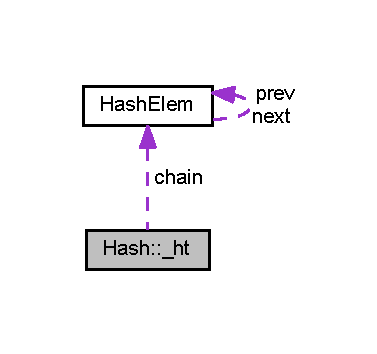
\includegraphics[width=181pt]{struct_hash_1_1__ht__coll__graph}
\end{center}
\end{figure}
\subsection*{Public Attributes}
\begin{DoxyCompactItemize}
\item 
\hypertarget{struct_hash_1_1__ht_a0677191178b6c7c5c6c2880f41cf24b1}{int {\bfseries count}}\label{struct_hash_1_1__ht_a0677191178b6c7c5c6c2880f41cf24b1}

\item 
\hypertarget{struct_hash_1_1__ht_a56fc145e7d38d9440d85ab2ea63a48ac}{\hyperlink{struct_hash_elem}{Hash\-Elem} $\ast$ {\bfseries chain}}\label{struct_hash_1_1__ht_a56fc145e7d38d9440d85ab2ea63a48ac}

\end{DoxyCompactItemize}


The documentation for this struct was generated from the following file\-:\begin{DoxyCompactItemize}
\item 
C\-:/\-Users/\-Vitor/\-Desktop/\-Work\-Space/\-P\-R\-O\-J\-E\-T\-O\-\_\-\-F\-I\-N\-A\-L\-\_\-\-P\-O\-O/\-P\-R\-O\-J\-E\-T\-O\-\_\-\-D\-E\-V/\-P\-R\-O\-J\-E\-T\-O/\-Projeto\-\_\-codeblocks/sqlite3.\-c\end{DoxyCompactItemize}

\hypertarget{struct_mem_page_1_1___ovfl_cell}{\section{Mem\-Page\-:\-:\-\_\-\-Ovfl\-Cell Struct Reference}
\label{struct_mem_page_1_1___ovfl_cell}\index{Mem\-Page\-::\-\_\-\-Ovfl\-Cell@{Mem\-Page\-::\-\_\-\-Ovfl\-Cell}}
}
\subsection*{Public Attributes}
\begin{DoxyCompactItemize}
\item 
\hypertarget{struct_mem_page_1_1___ovfl_cell_a75c64097a5af396bbdc30e859f33a7c9}{u8 $\ast$ {\bfseries p\-Cell}}\label{struct_mem_page_1_1___ovfl_cell_a75c64097a5af396bbdc30e859f33a7c9}

\item 
\hypertarget{struct_mem_page_1_1___ovfl_cell_ad10c93756d29693601aa63923a7fbee3}{u16 {\bfseries idx}}\label{struct_mem_page_1_1___ovfl_cell_ad10c93756d29693601aa63923a7fbee3}

\end{DoxyCompactItemize}


The documentation for this struct was generated from the following file\-:\begin{DoxyCompactItemize}
\item 
C\-:/\-Users/\-Vitor/\-Desktop/\-Work\-Space/\-P\-R\-O\-J\-E\-T\-O\-\_\-\-F\-I\-N\-A\-L\-\_\-\-P\-O\-O/\-P\-R\-O\-J\-E\-T\-O\-\_\-\-D\-E\-V/\-P\-R\-O\-J\-E\-T\-O/\-Projeto\-\_\-codeblocks/sqlite3.\-c\end{DoxyCompactItemize}

\hypertarget{class_a_commad}{\section{A\-Commad Class Reference}
\label{class_a_commad}\index{A\-Commad@{A\-Commad}}
}


Esse e a classe abstrata de comandos.  




{\ttfamily \#include $<$Comand.\-h$>$}



\subsection{Detailed Description}
Esse e a classe abstrata de comandos. 

The documentation for this class was generated from the following file\-:\begin{DoxyCompactItemize}
\item 
C\-:/\-Users/\-Vitor/\-Desktop/\-Work\-Space/\-P\-R\-O\-J\-E\-T\-O\-\_\-\-F\-I\-N\-A\-L\-\_\-\-P\-O\-O/\-P\-R\-O\-J\-E\-T\-O\-\_\-\-D\-E\-V/\-P\-R\-O\-J\-E\-T\-O/\-Projeto\-\_\-codeblocks/Comand.\-h\end{DoxyCompactItemize}

\hypertarget{class_a_command}{\section{A\-Command Class Reference}
\label{class_a_command}\index{A\-Command@{A\-Command}}
}


Essa é a classe abstrata de comandos da persistência.  




{\ttfamily \#include $<$Comand.\-h$>$}



Inheritance diagram for A\-Command\-:\nopagebreak
\begin{figure}[H]
\begin{center}
\leavevmode
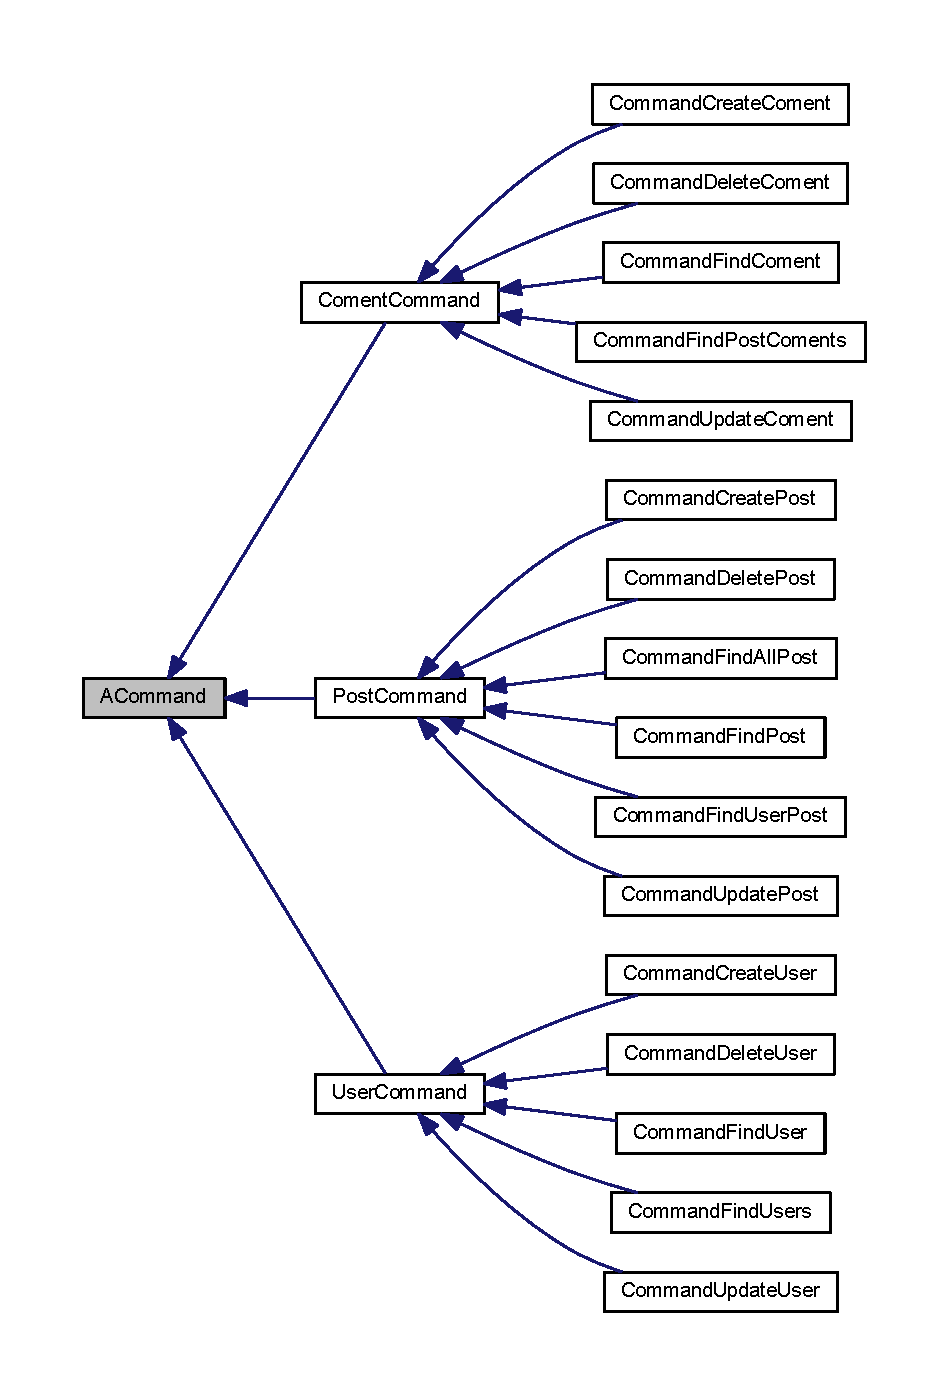
\includegraphics[width=350pt]{class_a_command__inherit__graph}
\end{center}
\end{figure}


Collaboration diagram for A\-Command\-:\nopagebreak
\begin{figure}[H]
\begin{center}
\leavevmode
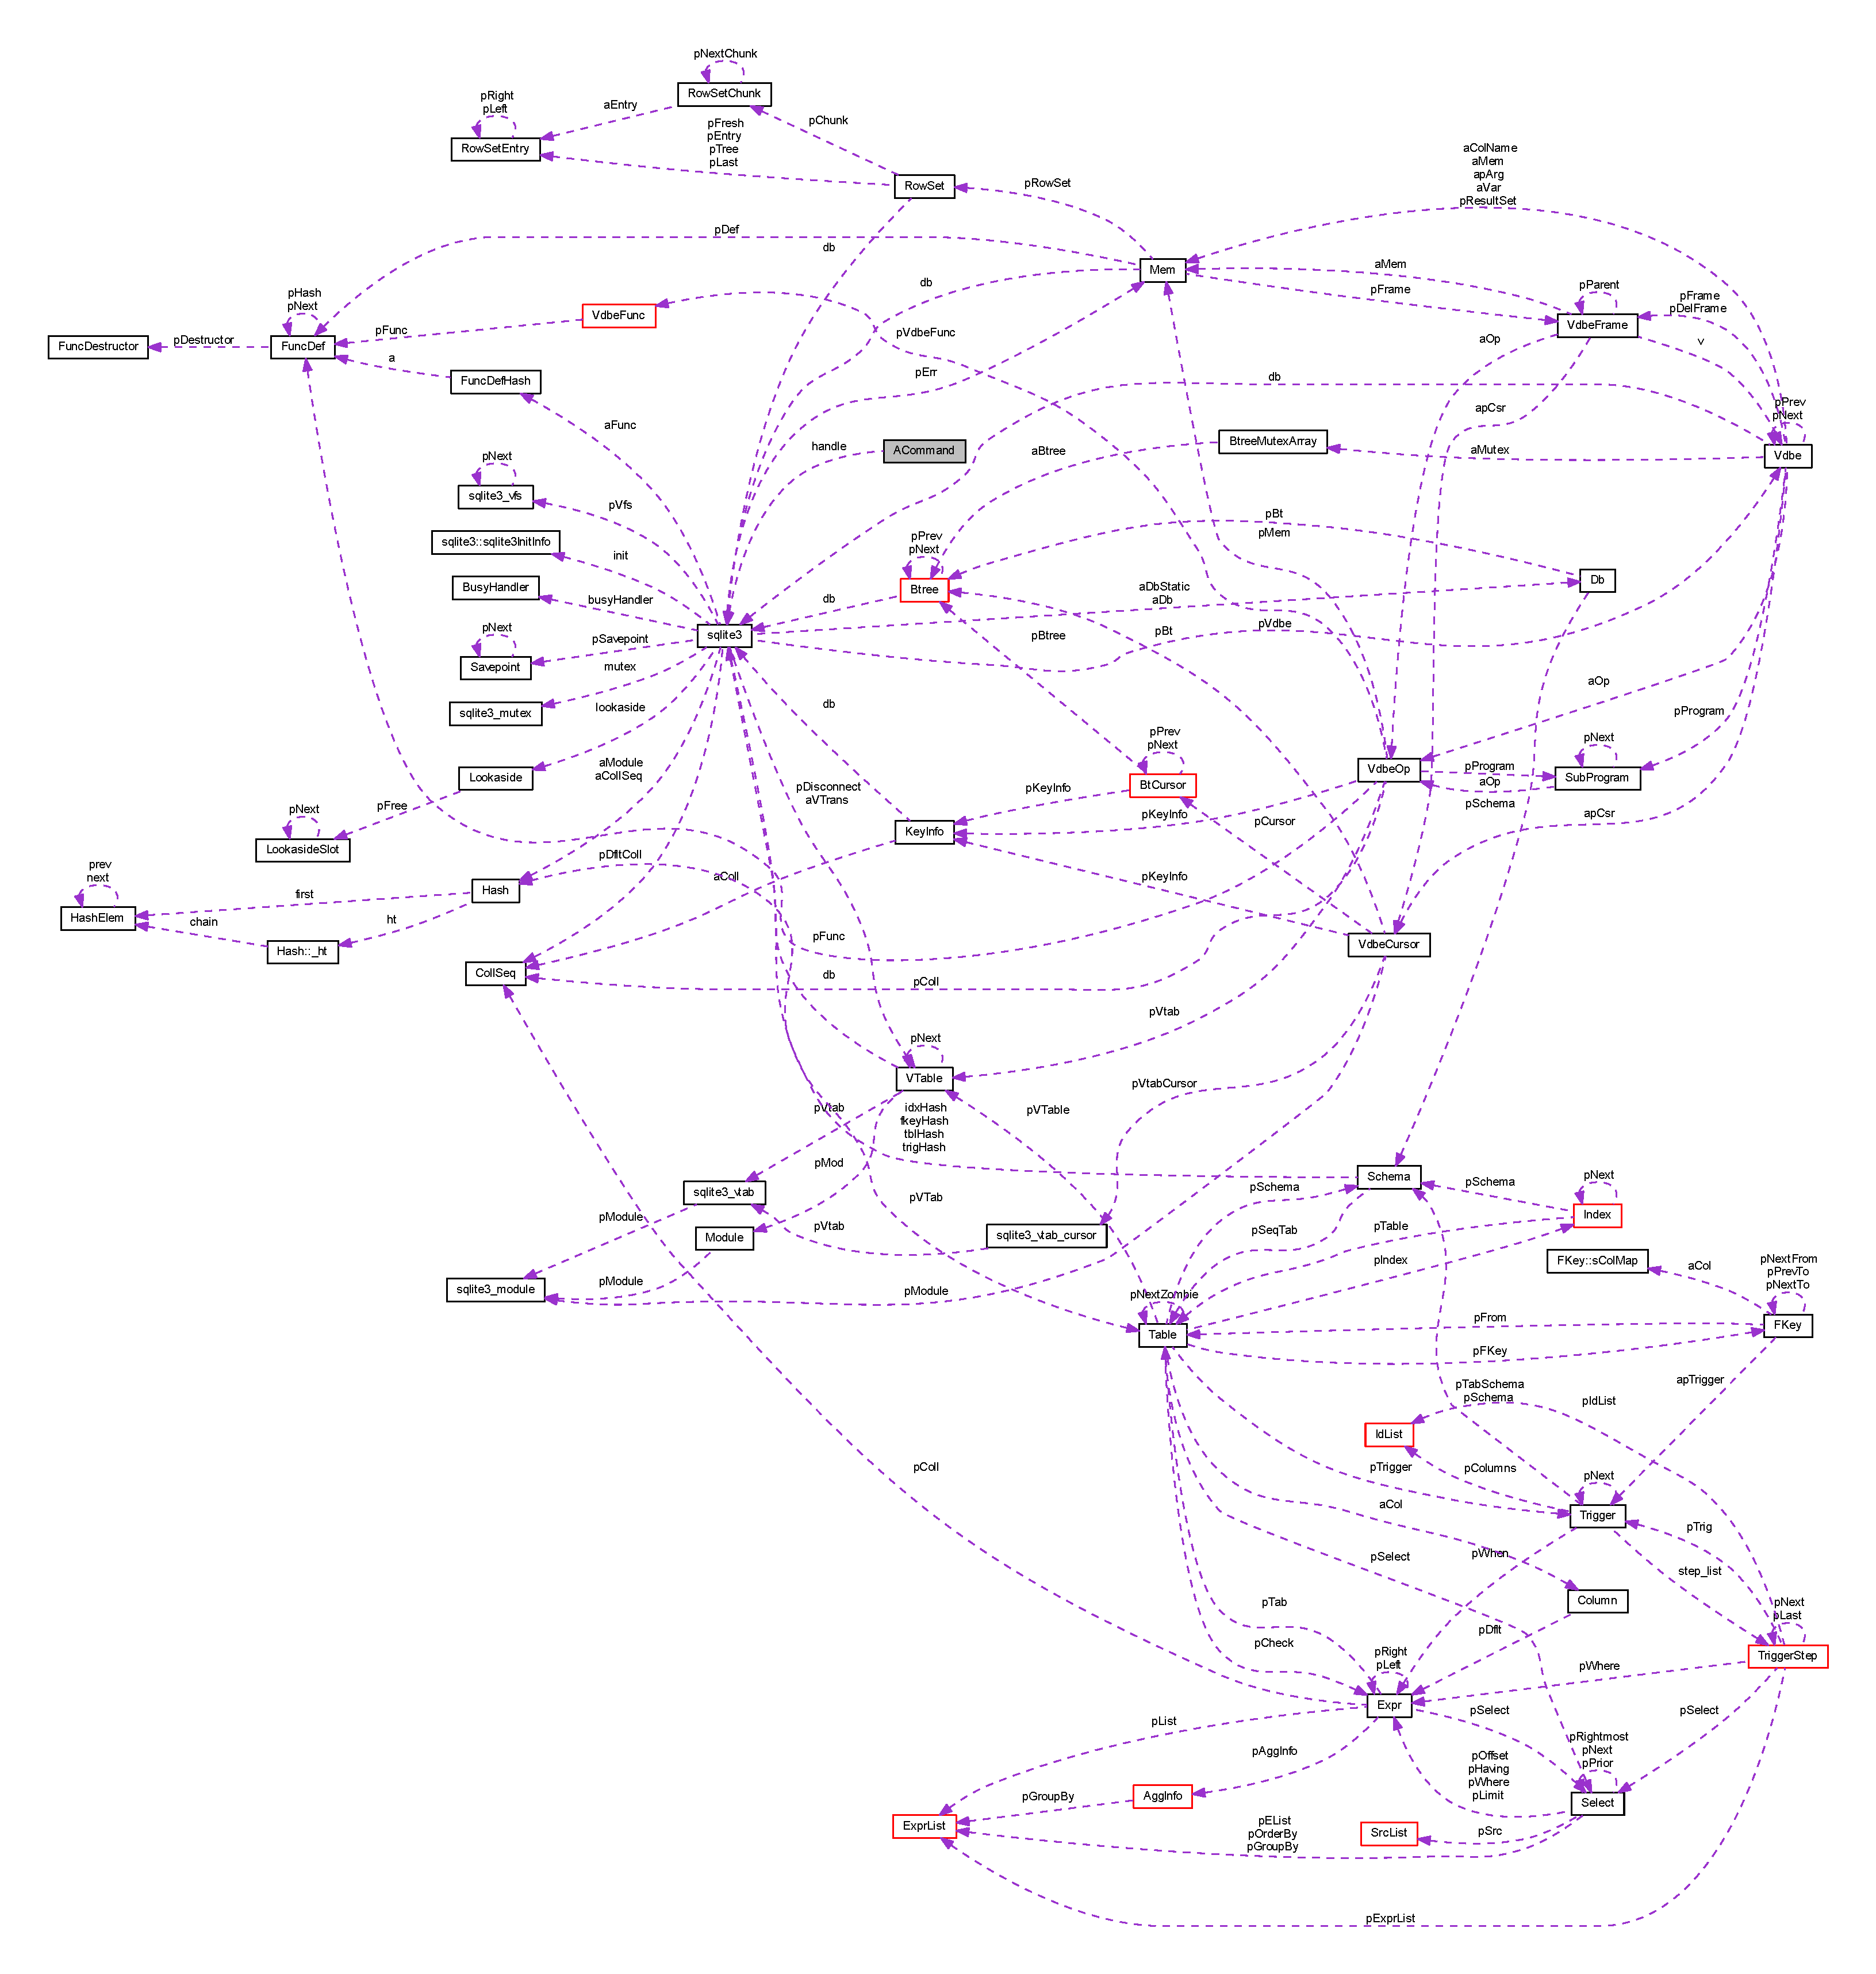
\includegraphics[width=350pt]{class_a_command__coll__graph}
\end{center}
\end{figure}
\subsection*{Public Member Functions}
\begin{DoxyCompactItemize}
\item 
\hypertarget{class_a_command_a94c6a1d25eb0427389e15450019ebad8}{virtual void \hyperlink{class_a_command_a94c6a1d25eb0427389e15450019ebad8}{execute} ()=0}\label{class_a_command_a94c6a1d25eb0427389e15450019ebad8}

\begin{DoxyCompactList}\small\item\em Método responsável por iniciar a execução da classe. \end{DoxyCompactList}\end{DoxyCompactItemize}
\subsection*{Protected Member Functions}
\begin{DoxyCompactItemize}
\item 
\hypertarget{class_a_command_a7ef6229ca895b6c264d4e466c08fe331}{void \hyperlink{class_a_command_a7ef6229ca895b6c264d4e466c08fe331}{conect} ()}\label{class_a_command_a7ef6229ca895b6c264d4e466c08fe331}

\begin{DoxyCompactList}\small\item\em Método responsável por conectar do banco de dados. \end{DoxyCompactList}\item 
\hypertarget{class_a_command_a07aaf5d1dd0efacfd9512154db5a845e}{void \hyperlink{class_a_command_a07aaf5d1dd0efacfd9512154db5a845e}{desconect} ()}\label{class_a_command_a07aaf5d1dd0efacfd9512154db5a845e}

\begin{DoxyCompactList}\small\item\em Método responsável por desconectar do banco de dados. \end{DoxyCompactList}\end{DoxyCompactItemize}
\subsection*{Protected Attributes}
\begin{DoxyCompactItemize}
\item 
\hypertarget{class_a_command_a8047bfd0b2365b5e82cfae6f4a894ce1}{char $\ast$ {\bfseries sql}}\label{class_a_command_a8047bfd0b2365b5e82cfae6f4a894ce1}

\item 
char $\ast$ \hyperlink{class_a_command_ac36454f9da108ff845c6303c8d7f70ae}{end}
\item 
\hypertarget{class_a_command_a435e761a4eb4fa339a0669a53430bd52}{int {\bfseries retval}}\label{class_a_command_a435e761a4eb4fa339a0669a53430bd52}

\item 
int \hyperlink{class_a_command_aa011a4976cefd5da8bd7e8231809f19d}{i}
\item 
\hypertarget{class_a_command_a41a087661bd8e5f7e7ff029ebddb3978}{int {\bfseries q\-\_\-cnt}}\label{class_a_command_a41a087661bd8e5f7e7ff029ebddb3978}

\item 
int \hyperlink{class_a_command_a769e24f33dec6fbffac667052257d575}{q\-\_\-size}
\item 
char $\ast$$\ast$ \hyperlink{class_a_command_a6a34b07a8ab76688ad3a60bfba71c03a}{queries}
\item 
char \hyperlink{class_a_command_a92ecbf13bd3238cd74125505954d211f}{valida\-\_\-name} \mbox{[}11\mbox{]}
\item 
sqlite3\-\_\-stmt $\ast$ \hyperlink{class_a_command_a7ecdb33c925dc75b9538a4009ff88c6c}{stmt}
\item 
\hyperlink{structsqlite3}{sqlite3} $\ast$ \hyperlink{class_a_command_a6f48bd41253cbcc5e766c222776e4931}{handle}
\end{DoxyCompactItemize}


\subsection{Detailed Description}
Essa é a classe abstrata de comandos da persistência. 

\subsection{Member Data Documentation}
\hypertarget{class_a_command_ac36454f9da108ff845c6303c8d7f70ae}{\index{A\-Command@{A\-Command}!end@{end}}
\index{end@{end}!ACommand@{A\-Command}}
\subsubsection[{end}]{\setlength{\rightskip}{0pt plus 5cm}char $\ast$ A\-Command\-::end\hspace{0.3cm}{\ttfamily [protected]}}}\label{class_a_command_ac36454f9da108ff845c6303c8d7f70ae}
Variavel que armazena o comando a ser realizado em sqp Variavel que serve para finalizar o B\-D \hypertarget{class_a_command_a6f48bd41253cbcc5e766c222776e4931}{\index{A\-Command@{A\-Command}!handle@{handle}}
\index{handle@{handle}!ACommand@{A\-Command}}
\subsubsection[{handle}]{\setlength{\rightskip}{0pt plus 5cm}{\bf sqlite3}$\ast$ A\-Command\-::handle\hspace{0.3cm}{\ttfamily [protected]}}}\label{class_a_command_a6f48bd41253cbcc5e766c222776e4931}
Variavel que armazena o o banco de dados \hypertarget{class_a_command_aa011a4976cefd5da8bd7e8231809f19d}{\index{A\-Command@{A\-Command}!i@{i}}
\index{i@{i}!ACommand@{A\-Command}}
\subsubsection[{i}]{\setlength{\rightskip}{0pt plus 5cm}int A\-Command\-::i\hspace{0.3cm}{\ttfamily [protected]}}}\label{class_a_command_aa011a4976cefd5da8bd7e8231809f19d}
Variavel que verifica se tudo ocorreu bem Contador \hypertarget{class_a_command_a769e24f33dec6fbffac667052257d575}{\index{A\-Command@{A\-Command}!q\-\_\-size@{q\-\_\-size}}
\index{q\-\_\-size@{q\-\_\-size}!ACommand@{A\-Command}}
\subsubsection[{q\-\_\-size}]{\setlength{\rightskip}{0pt plus 5cm}int A\-Command\-::q\-\_\-size\hspace{0.3cm}{\ttfamily [protected]}}}\label{class_a_command_a769e24f33dec6fbffac667052257d575}
Variavel que armazena o identificador unico do Usuario Variavel que armazena o identificador unico do Usuario \hypertarget{class_a_command_a6a34b07a8ab76688ad3a60bfba71c03a}{\index{A\-Command@{A\-Command}!queries@{queries}}
\index{queries@{queries}!ACommand@{A\-Command}}
\subsubsection[{queries}]{\setlength{\rightskip}{0pt plus 5cm}char$\ast$$\ast$ A\-Command\-::queries\hspace{0.3cm}{\ttfamily [protected]}}}\label{class_a_command_a6a34b07a8ab76688ad3a60bfba71c03a}
Variavel que armazena as consultas \hypertarget{class_a_command_a7ecdb33c925dc75b9538a4009ff88c6c}{\index{A\-Command@{A\-Command}!stmt@{stmt}}
\index{stmt@{stmt}!ACommand@{A\-Command}}
\subsubsection[{stmt}]{\setlength{\rightskip}{0pt plus 5cm}sqlite3\-\_\-stmt$\ast$ A\-Command\-::stmt\hspace{0.3cm}{\ttfamily [protected]}}}\label{class_a_command_a7ecdb33c925dc75b9538a4009ff88c6c}
Variavel que armazena algo escrito \hypertarget{class_a_command_a92ecbf13bd3238cd74125505954d211f}{\index{A\-Command@{A\-Command}!valida\-\_\-name@{valida\-\_\-name}}
\index{valida\-\_\-name@{valida\-\_\-name}!ACommand@{A\-Command}}
\subsubsection[{valida\-\_\-name}]{\setlength{\rightskip}{0pt plus 5cm}char A\-Command\-::valida\-\_\-name\mbox{[}11\mbox{]}\hspace{0.3cm}{\ttfamily [protected]}}}\label{class_a_command_a92ecbf13bd3238cd74125505954d211f}
Variavel para validar se um nome já existi 

The documentation for this class was generated from the following files\-:\begin{DoxyCompactItemize}
\item 
Comand.\-h\item 
Comand.\-cpp\end{DoxyCompactItemize}

\hypertarget{struct_agg_info}{\section{Agg\-Info Struct Reference}
\label{struct_agg_info}\index{Agg\-Info@{Agg\-Info}}
}


Collaboration diagram for Agg\-Info\-:\nopagebreak
\begin{figure}[H]
\begin{center}
\leavevmode
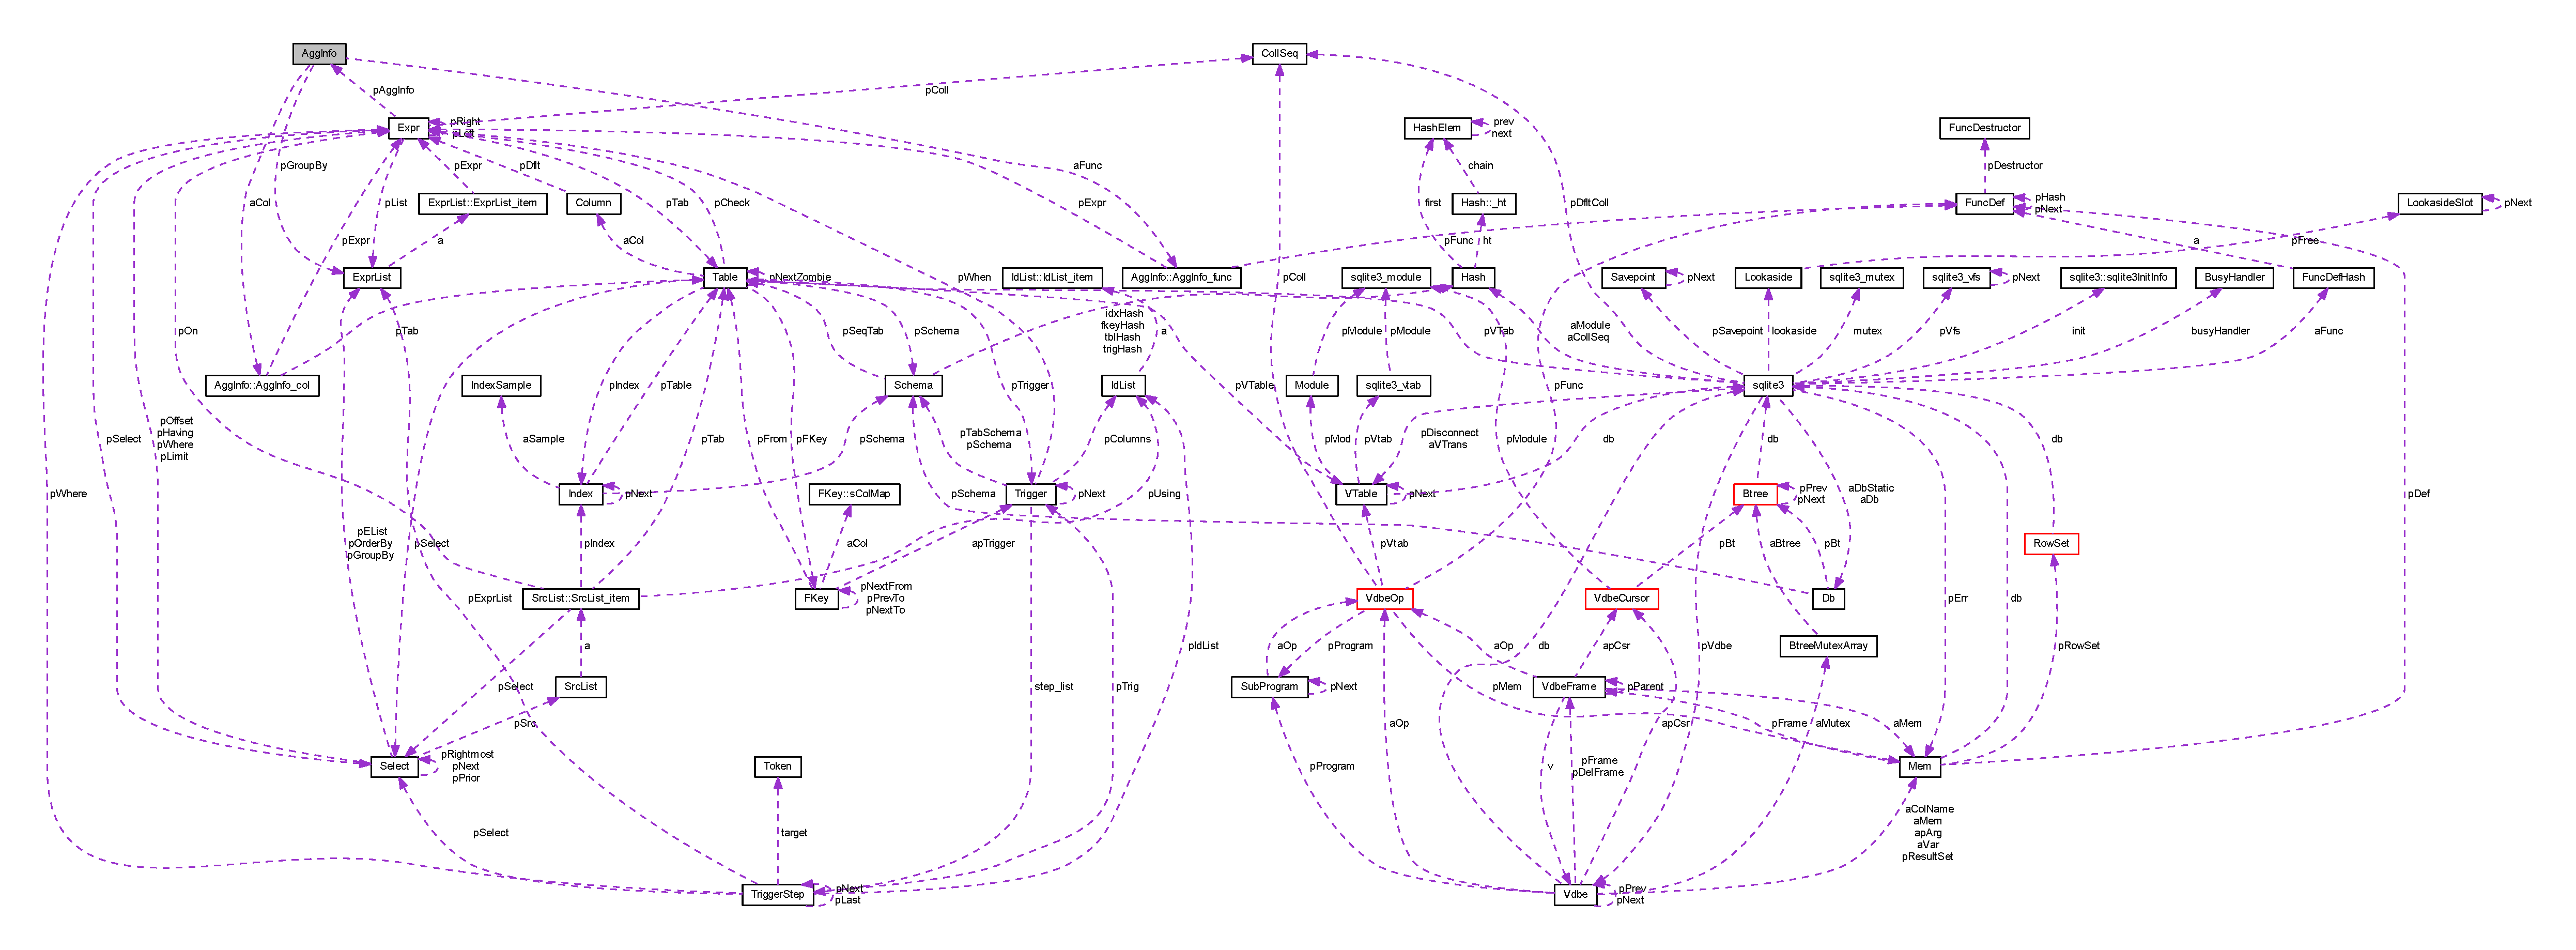
\includegraphics[width=350pt]{struct_agg_info__coll__graph}
\end{center}
\end{figure}
\subsection*{Classes}
\begin{DoxyCompactItemize}
\item 
struct \hyperlink{struct_agg_info_1_1_agg_info__col}{Agg\-Info\-\_\-col}
\item 
struct \hyperlink{struct_agg_info_1_1_agg_info__func}{Agg\-Info\-\_\-func}
\end{DoxyCompactItemize}
\subsection*{Public Attributes}
\begin{DoxyCompactItemize}
\item 
\hypertarget{struct_agg_info_aaa57d294016ac7e17e7cacaa7b25634e}{u8 {\bfseries direct\-Mode}}\label{struct_agg_info_aaa57d294016ac7e17e7cacaa7b25634e}

\item 
\hypertarget{struct_agg_info_a8173a7ea13c4a12ce4befbcb40719073}{u8 {\bfseries use\-Sorting\-Idx}}\label{struct_agg_info_a8173a7ea13c4a12ce4befbcb40719073}

\item 
\hypertarget{struct_agg_info_a97ce74f509ca908a616c123e7196797b}{int {\bfseries sorting\-Idx}}\label{struct_agg_info_a97ce74f509ca908a616c123e7196797b}

\item 
\hypertarget{struct_agg_info_aa8e942103d224c4db847743670907781}{\hyperlink{struct_expr_list}{Expr\-List} $\ast$ {\bfseries p\-Group\-By}}\label{struct_agg_info_aa8e942103d224c4db847743670907781}

\item 
\hypertarget{struct_agg_info_a89925dccd1a0ec51d2a5a5dbaead66dc}{int {\bfseries n\-Sorting\-Column}}\label{struct_agg_info_a89925dccd1a0ec51d2a5a5dbaead66dc}

\item 
\hypertarget{struct_agg_info_a52fa1a7eb3145c27be13b2bcccd57d62}{struct \hyperlink{struct_agg_info_1_1_agg_info__col}{Agg\-Info\-::\-Agg\-Info\-\_\-col} $\ast$ {\bfseries a\-Col}}\label{struct_agg_info_a52fa1a7eb3145c27be13b2bcccd57d62}

\item 
\hypertarget{struct_agg_info_a9cbfa5fc33328cf3500426674e036a8b}{int {\bfseries n\-Column}}\label{struct_agg_info_a9cbfa5fc33328cf3500426674e036a8b}

\item 
\hypertarget{struct_agg_info_a2d826c17800c21fd27952545993227c7}{int {\bfseries n\-Column\-Alloc}}\label{struct_agg_info_a2d826c17800c21fd27952545993227c7}

\item 
\hypertarget{struct_agg_info_ad2251760d95af9024f0a3170405cb53b}{int {\bfseries n\-Accumulator}}\label{struct_agg_info_ad2251760d95af9024f0a3170405cb53b}

\item 
\hypertarget{struct_agg_info_a4e201acd6a1f8aed360c58e45f47c803}{struct \hyperlink{struct_agg_info_1_1_agg_info__func}{Agg\-Info\-::\-Agg\-Info\-\_\-func} $\ast$ {\bfseries a\-Func}}\label{struct_agg_info_a4e201acd6a1f8aed360c58e45f47c803}

\item 
\hypertarget{struct_agg_info_a5bfde7ca00d28da6edbda523ab038e38}{int {\bfseries n\-Func}}\label{struct_agg_info_a5bfde7ca00d28da6edbda523ab038e38}

\item 
\hypertarget{struct_agg_info_a97c3bcfc404c3b328242c7698adacd05}{int {\bfseries n\-Func\-Alloc}}\label{struct_agg_info_a97c3bcfc404c3b328242c7698adacd05}

\end{DoxyCompactItemize}


The documentation for this struct was generated from the following file\-:\begin{DoxyCompactItemize}
\item 
C\-:/\-Users/\-Vitor/\-Desktop/\-Work\-Space/\-P\-R\-O\-J\-E\-T\-O\-\_\-\-F\-I\-N\-A\-L\-\_\-\-P\-O\-O/\-P\-R\-O\-J\-E\-T\-O\-\_\-\-D\-E\-V/\-P\-R\-O\-J\-E\-T\-O/\-Projeto\-\_\-codeblocks/sqlite3.\-c\end{DoxyCompactItemize}

\hypertarget{struct_agg_info_1_1_agg_info__col}{\section{Agg\-Info\-:\-:Agg\-Info\-\_\-col Struct Reference}
\label{struct_agg_info_1_1_agg_info__col}\index{Agg\-Info\-::\-Agg\-Info\-\_\-col@{Agg\-Info\-::\-Agg\-Info\-\_\-col}}
}


Collaboration diagram for Agg\-Info\-:\-:Agg\-Info\-\_\-col\-:\nopagebreak
\begin{figure}[H]
\begin{center}
\leavevmode
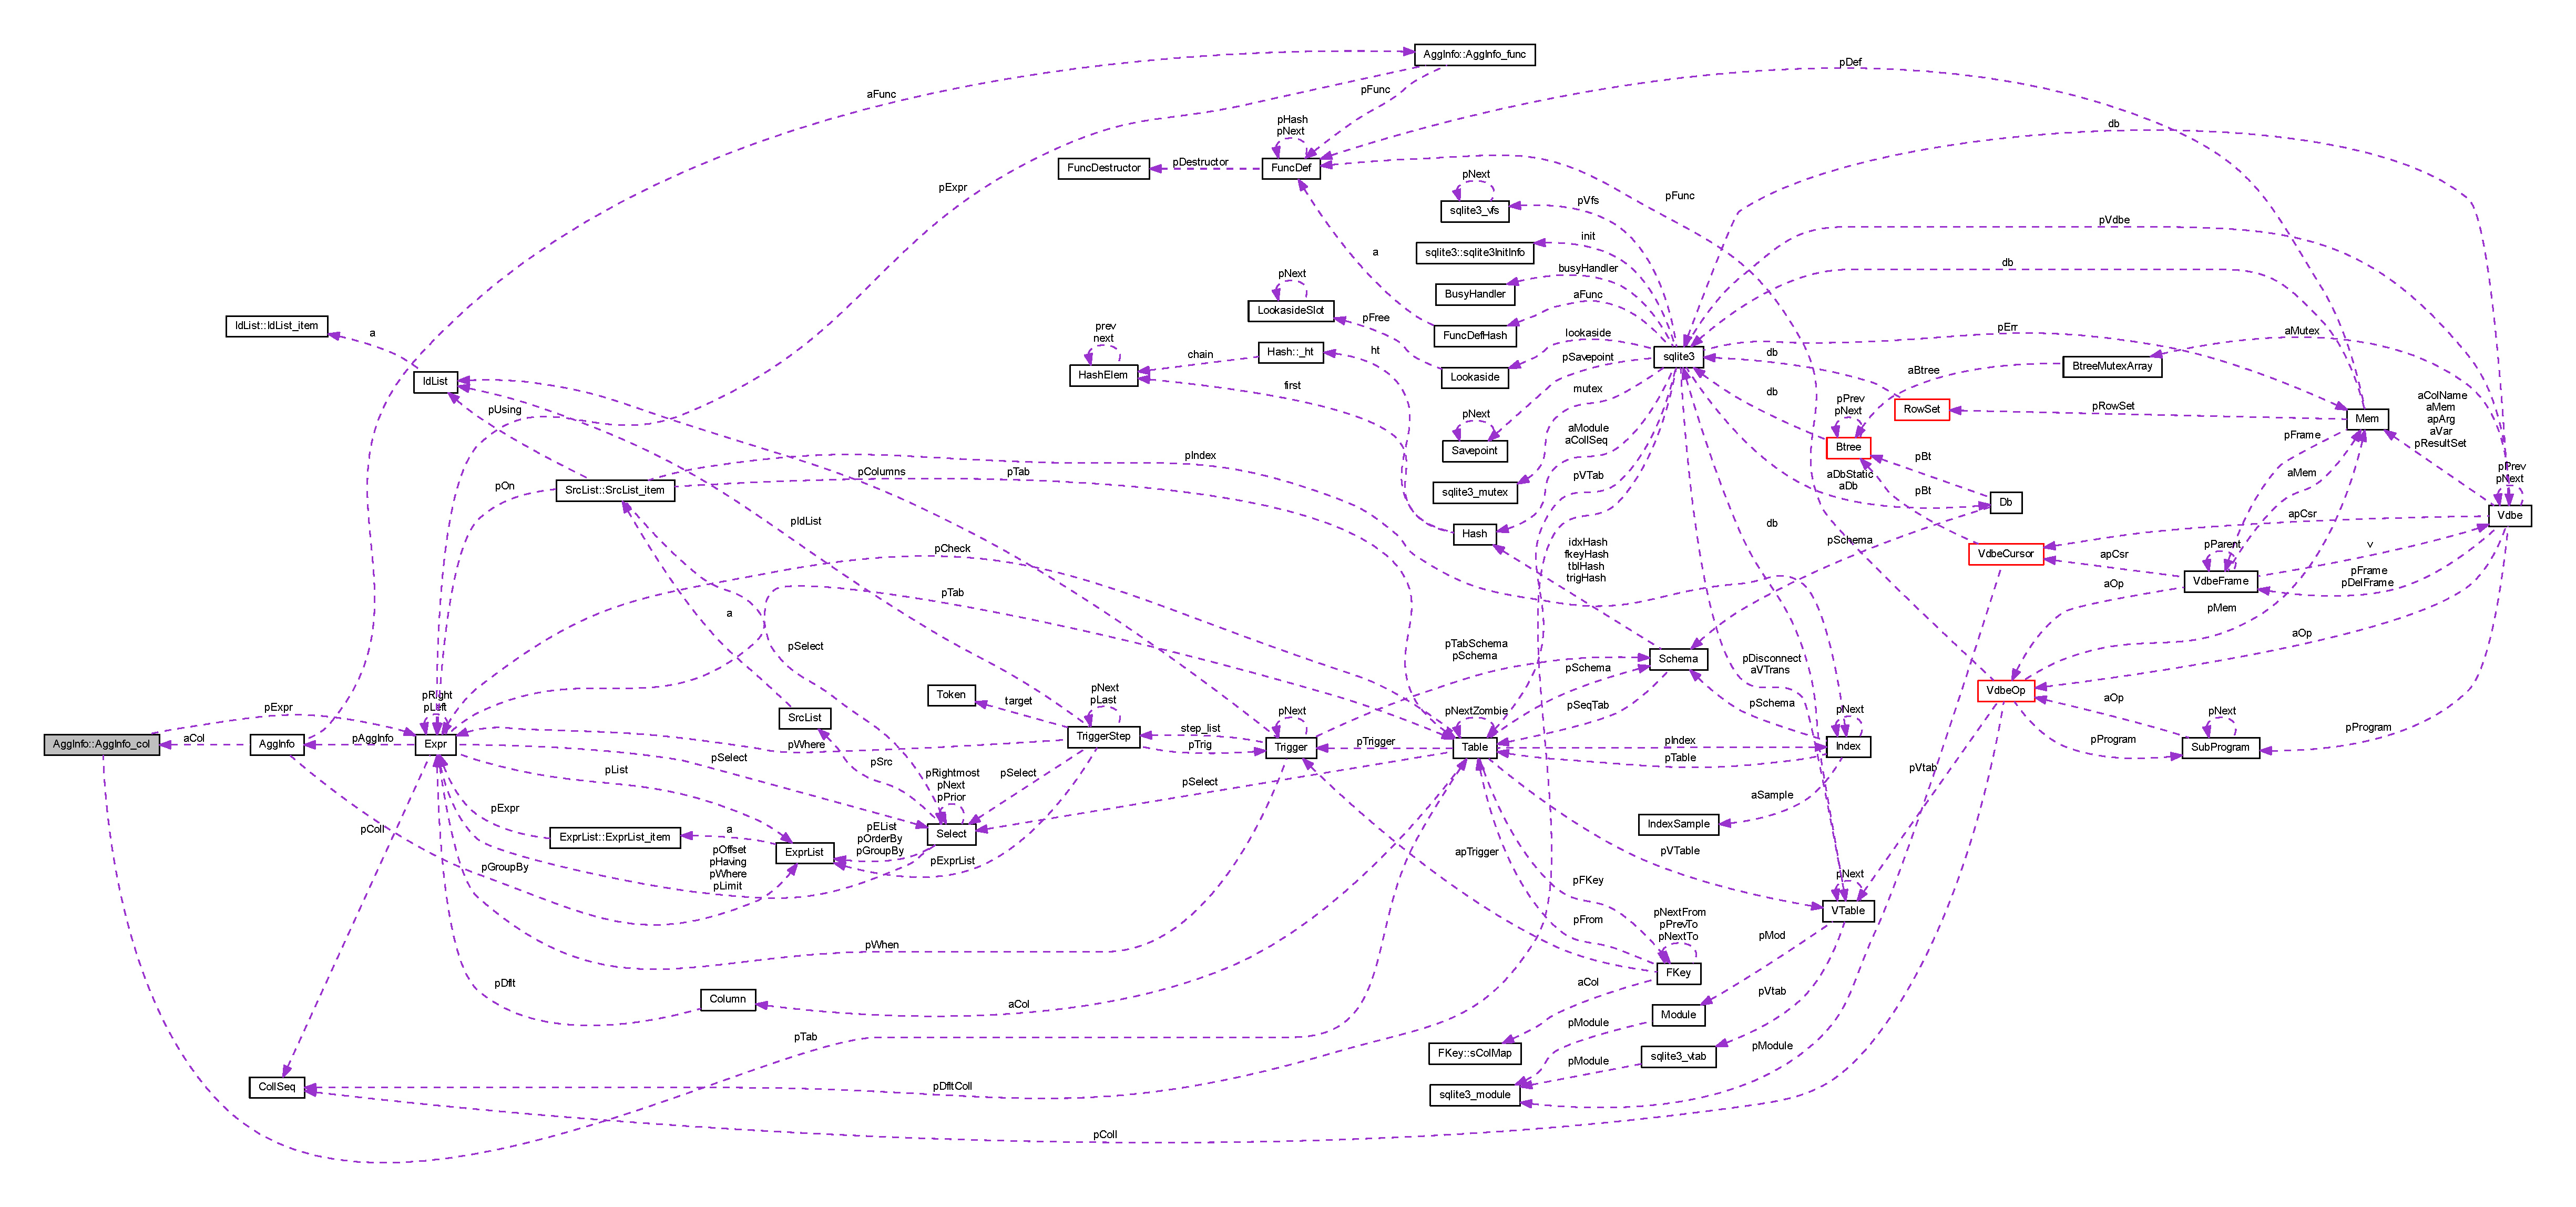
\includegraphics[width=350pt]{struct_agg_info_1_1_agg_info__col__coll__graph}
\end{center}
\end{figure}
\subsection*{Public Attributes}
\begin{DoxyCompactItemize}
\item 
\hypertarget{struct_agg_info_1_1_agg_info__col_ad2f2ae137b49e72d28a57accc9d06386}{\hyperlink{struct_table}{Table} $\ast$ {\bfseries p\-Tab}}\label{struct_agg_info_1_1_agg_info__col_ad2f2ae137b49e72d28a57accc9d06386}

\item 
\hypertarget{struct_agg_info_1_1_agg_info__col_ab49aa2fbfc6278c86b64497a6807c113}{int {\bfseries i\-Table}}\label{struct_agg_info_1_1_agg_info__col_ab49aa2fbfc6278c86b64497a6807c113}

\item 
\hypertarget{struct_agg_info_1_1_agg_info__col_a4cad2ce99ddf7425d358d49e40524f6b}{int {\bfseries i\-Column}}\label{struct_agg_info_1_1_agg_info__col_a4cad2ce99ddf7425d358d49e40524f6b}

\item 
\hypertarget{struct_agg_info_1_1_agg_info__col_ae3901ad0d5b6d519a7559358f1f7248b}{int {\bfseries i\-Sorter\-Column}}\label{struct_agg_info_1_1_agg_info__col_ae3901ad0d5b6d519a7559358f1f7248b}

\item 
\hypertarget{struct_agg_info_1_1_agg_info__col_ae22f3dfc6f9c2dc647be1b9fbd14e896}{int {\bfseries i\-Mem}}\label{struct_agg_info_1_1_agg_info__col_ae22f3dfc6f9c2dc647be1b9fbd14e896}

\item 
\hypertarget{struct_agg_info_1_1_agg_info__col_a60f23ec0abfcc88cab7083967a3abd9e}{\hyperlink{struct_expr}{Expr} $\ast$ {\bfseries p\-Expr}}\label{struct_agg_info_1_1_agg_info__col_a60f23ec0abfcc88cab7083967a3abd9e}

\end{DoxyCompactItemize}


The documentation for this struct was generated from the following file\-:\begin{DoxyCompactItemize}
\item 
C\-:/\-Users/\-Vitor/\-Desktop/\-Work\-Space/\-P\-R\-O\-J\-E\-T\-O\-\_\-\-F\-I\-N\-A\-L\-\_\-\-P\-O\-O/\-P\-R\-O\-J\-E\-T\-O\-\_\-\-D\-E\-V/\-P\-R\-O\-J\-E\-T\-O/\-Projeto\-\_\-codeblocks/sqlite3.\-c\end{DoxyCompactItemize}

\hypertarget{struct_agg_info_1_1_agg_info__func}{\section{Agg\-Info\-:\-:Agg\-Info\-\_\-func Struct Reference}
\label{struct_agg_info_1_1_agg_info__func}\index{Agg\-Info\-::\-Agg\-Info\-\_\-func@{Agg\-Info\-::\-Agg\-Info\-\_\-func}}
}


Collaboration diagram for Agg\-Info\-:\-:Agg\-Info\-\_\-func\-:\nopagebreak
\begin{figure}[H]
\begin{center}
\leavevmode
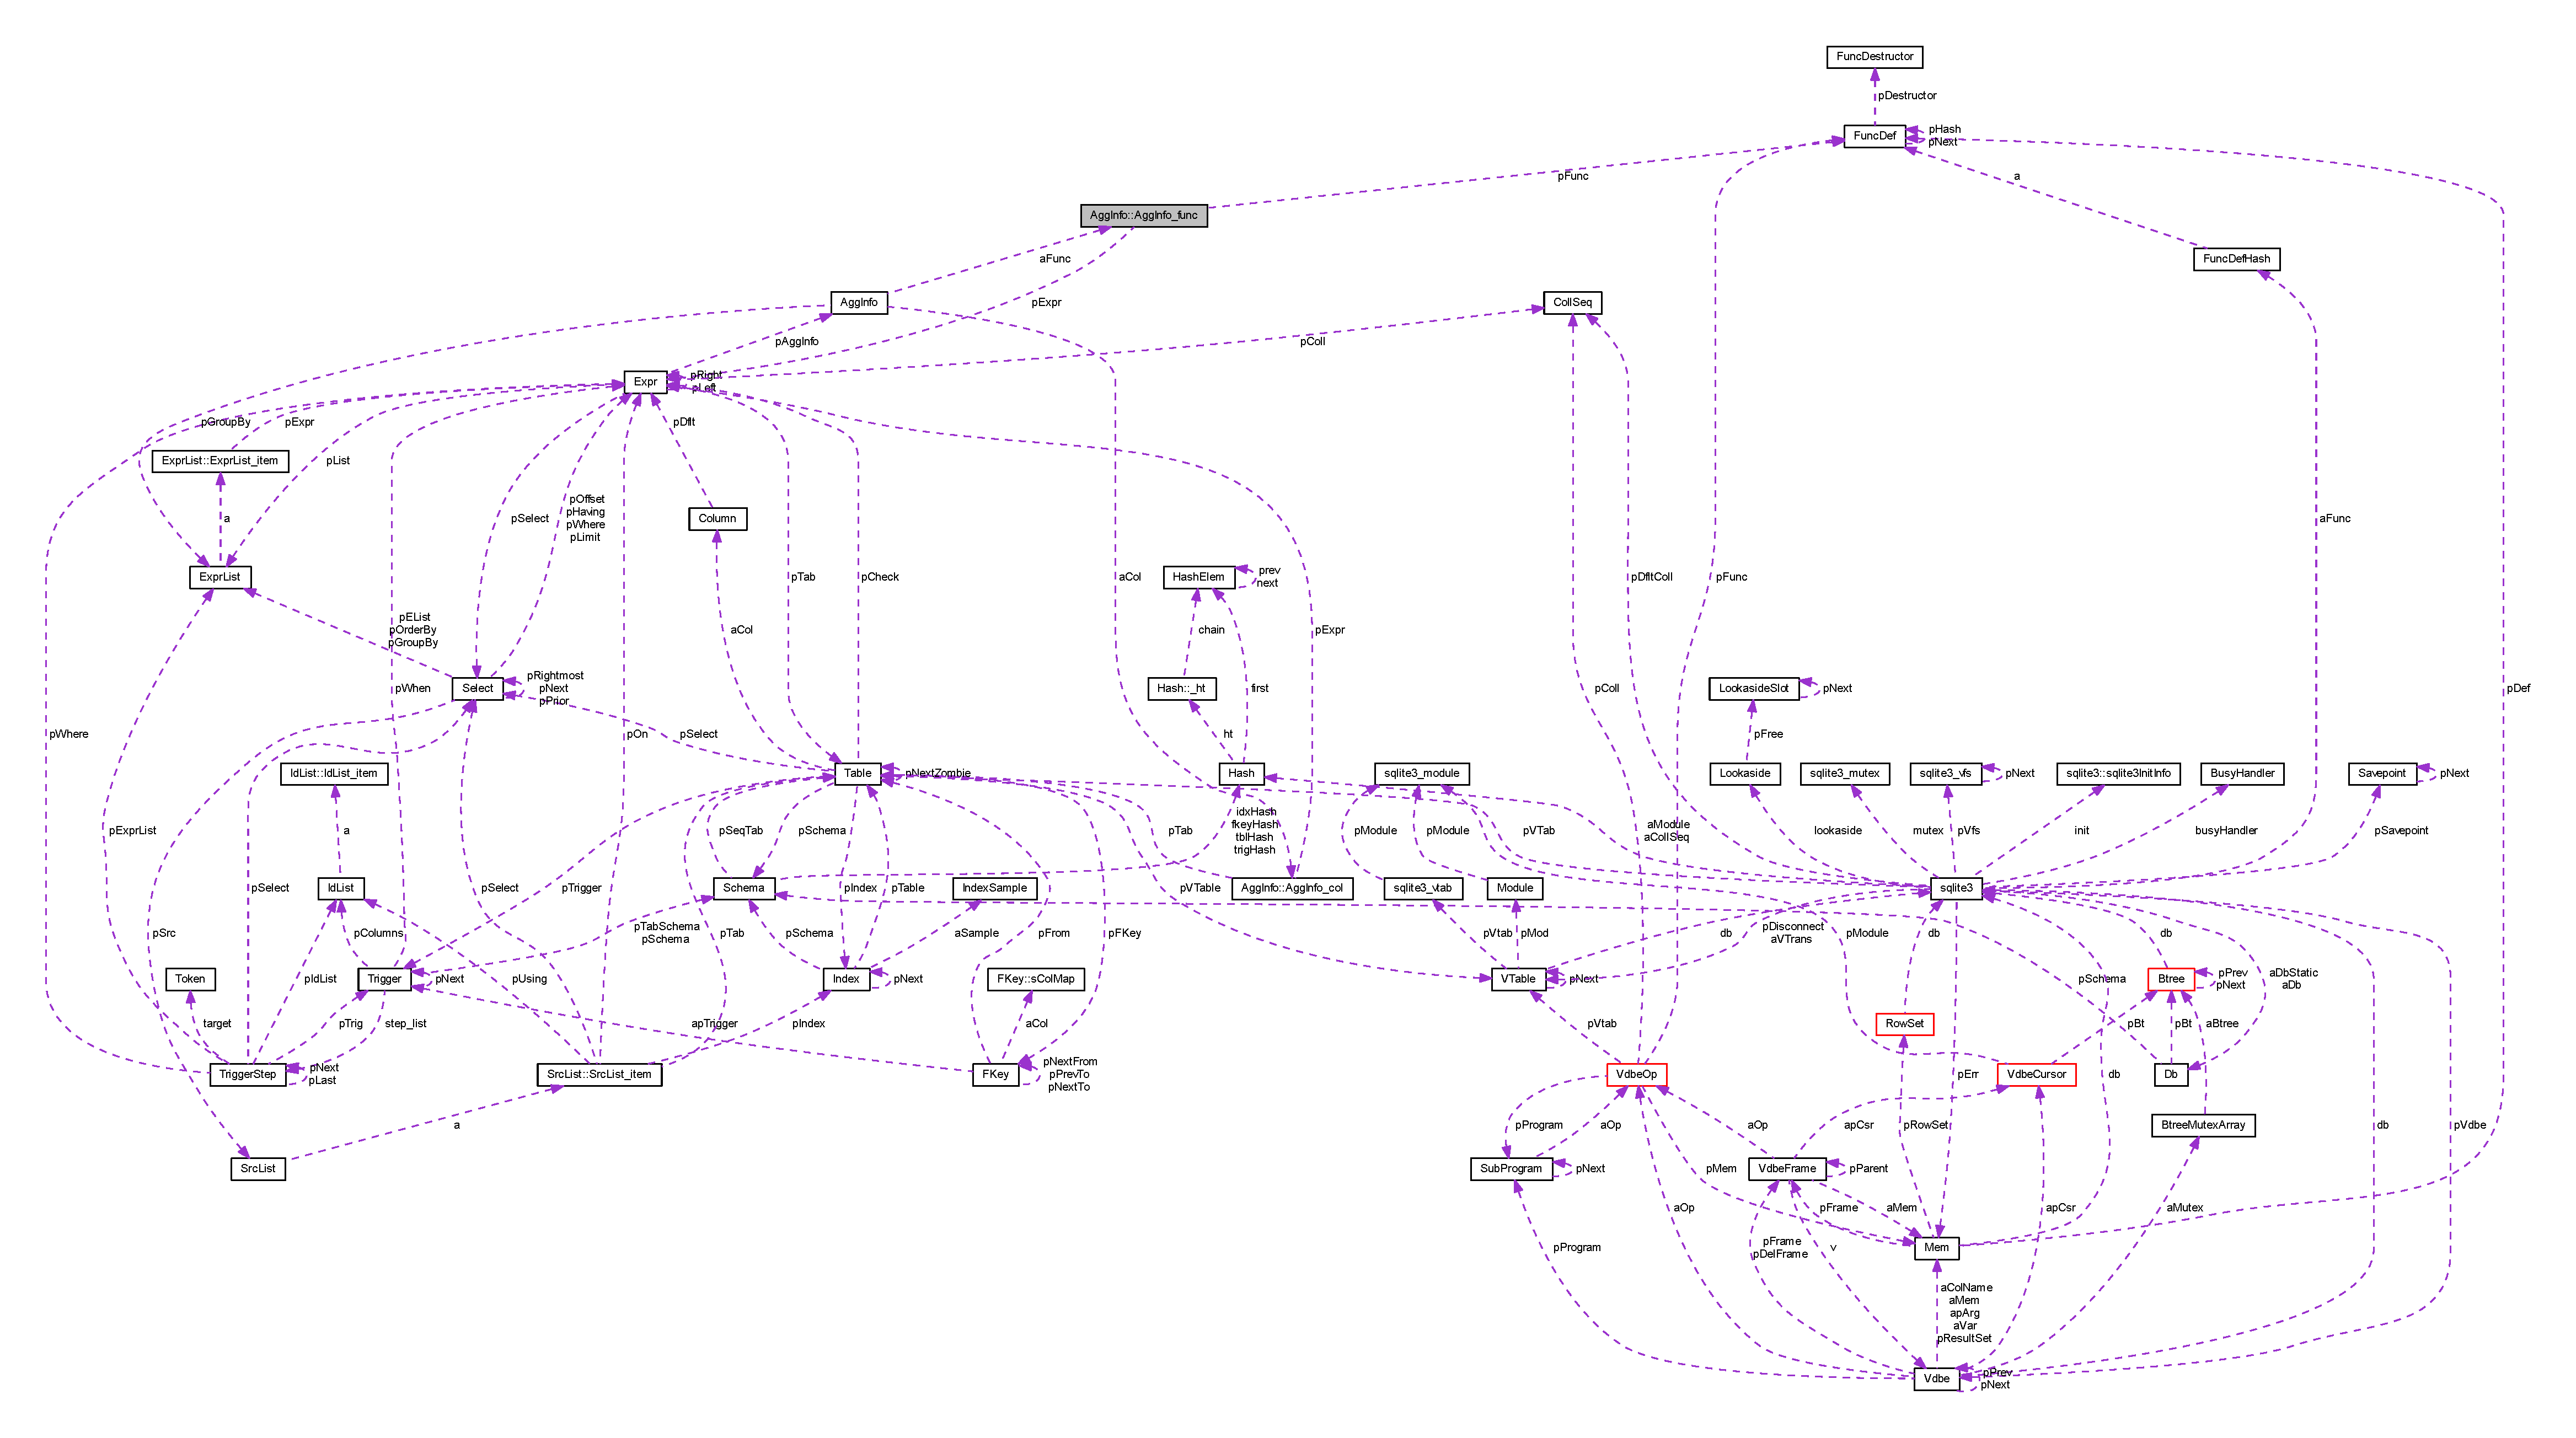
\includegraphics[width=350pt]{struct_agg_info_1_1_agg_info__func__coll__graph}
\end{center}
\end{figure}
\subsection*{Public Attributes}
\begin{DoxyCompactItemize}
\item 
\hypertarget{struct_agg_info_1_1_agg_info__func_a7b92e1c42e60d44e28ebf695316f4018}{\hyperlink{struct_expr}{Expr} $\ast$ {\bfseries p\-Expr}}\label{struct_agg_info_1_1_agg_info__func_a7b92e1c42e60d44e28ebf695316f4018}

\item 
\hypertarget{struct_agg_info_1_1_agg_info__func_a840478e8ec53cefa57b50228f6fdafe4}{\hyperlink{struct_func_def}{Func\-Def} $\ast$ {\bfseries p\-Func}}\label{struct_agg_info_1_1_agg_info__func_a840478e8ec53cefa57b50228f6fdafe4}

\item 
\hypertarget{struct_agg_info_1_1_agg_info__func_a41a8da36555c37fffc65f1acead49a4f}{int {\bfseries i\-Mem}}\label{struct_agg_info_1_1_agg_info__func_a41a8da36555c37fffc65f1acead49a4f}

\item 
\hypertarget{struct_agg_info_1_1_agg_info__func_a4a82635b0116eb44ec8ca9e47cc509d9}{int {\bfseries i\-Distinct}}\label{struct_agg_info_1_1_agg_info__func_a4a82635b0116eb44ec8ca9e47cc509d9}

\end{DoxyCompactItemize}


The documentation for this struct was generated from the following file\-:\begin{DoxyCompactItemize}
\item 
sqlite3.\-c\end{DoxyCompactItemize}

\hypertarget{structanalysis_info}{\section{analysis\-Info Struct Reference}
\label{structanalysis_info}\index{analysis\-Info@{analysis\-Info}}
}


Collaboration diagram for analysis\-Info\-:\nopagebreak
\begin{figure}[H]
\begin{center}
\leavevmode
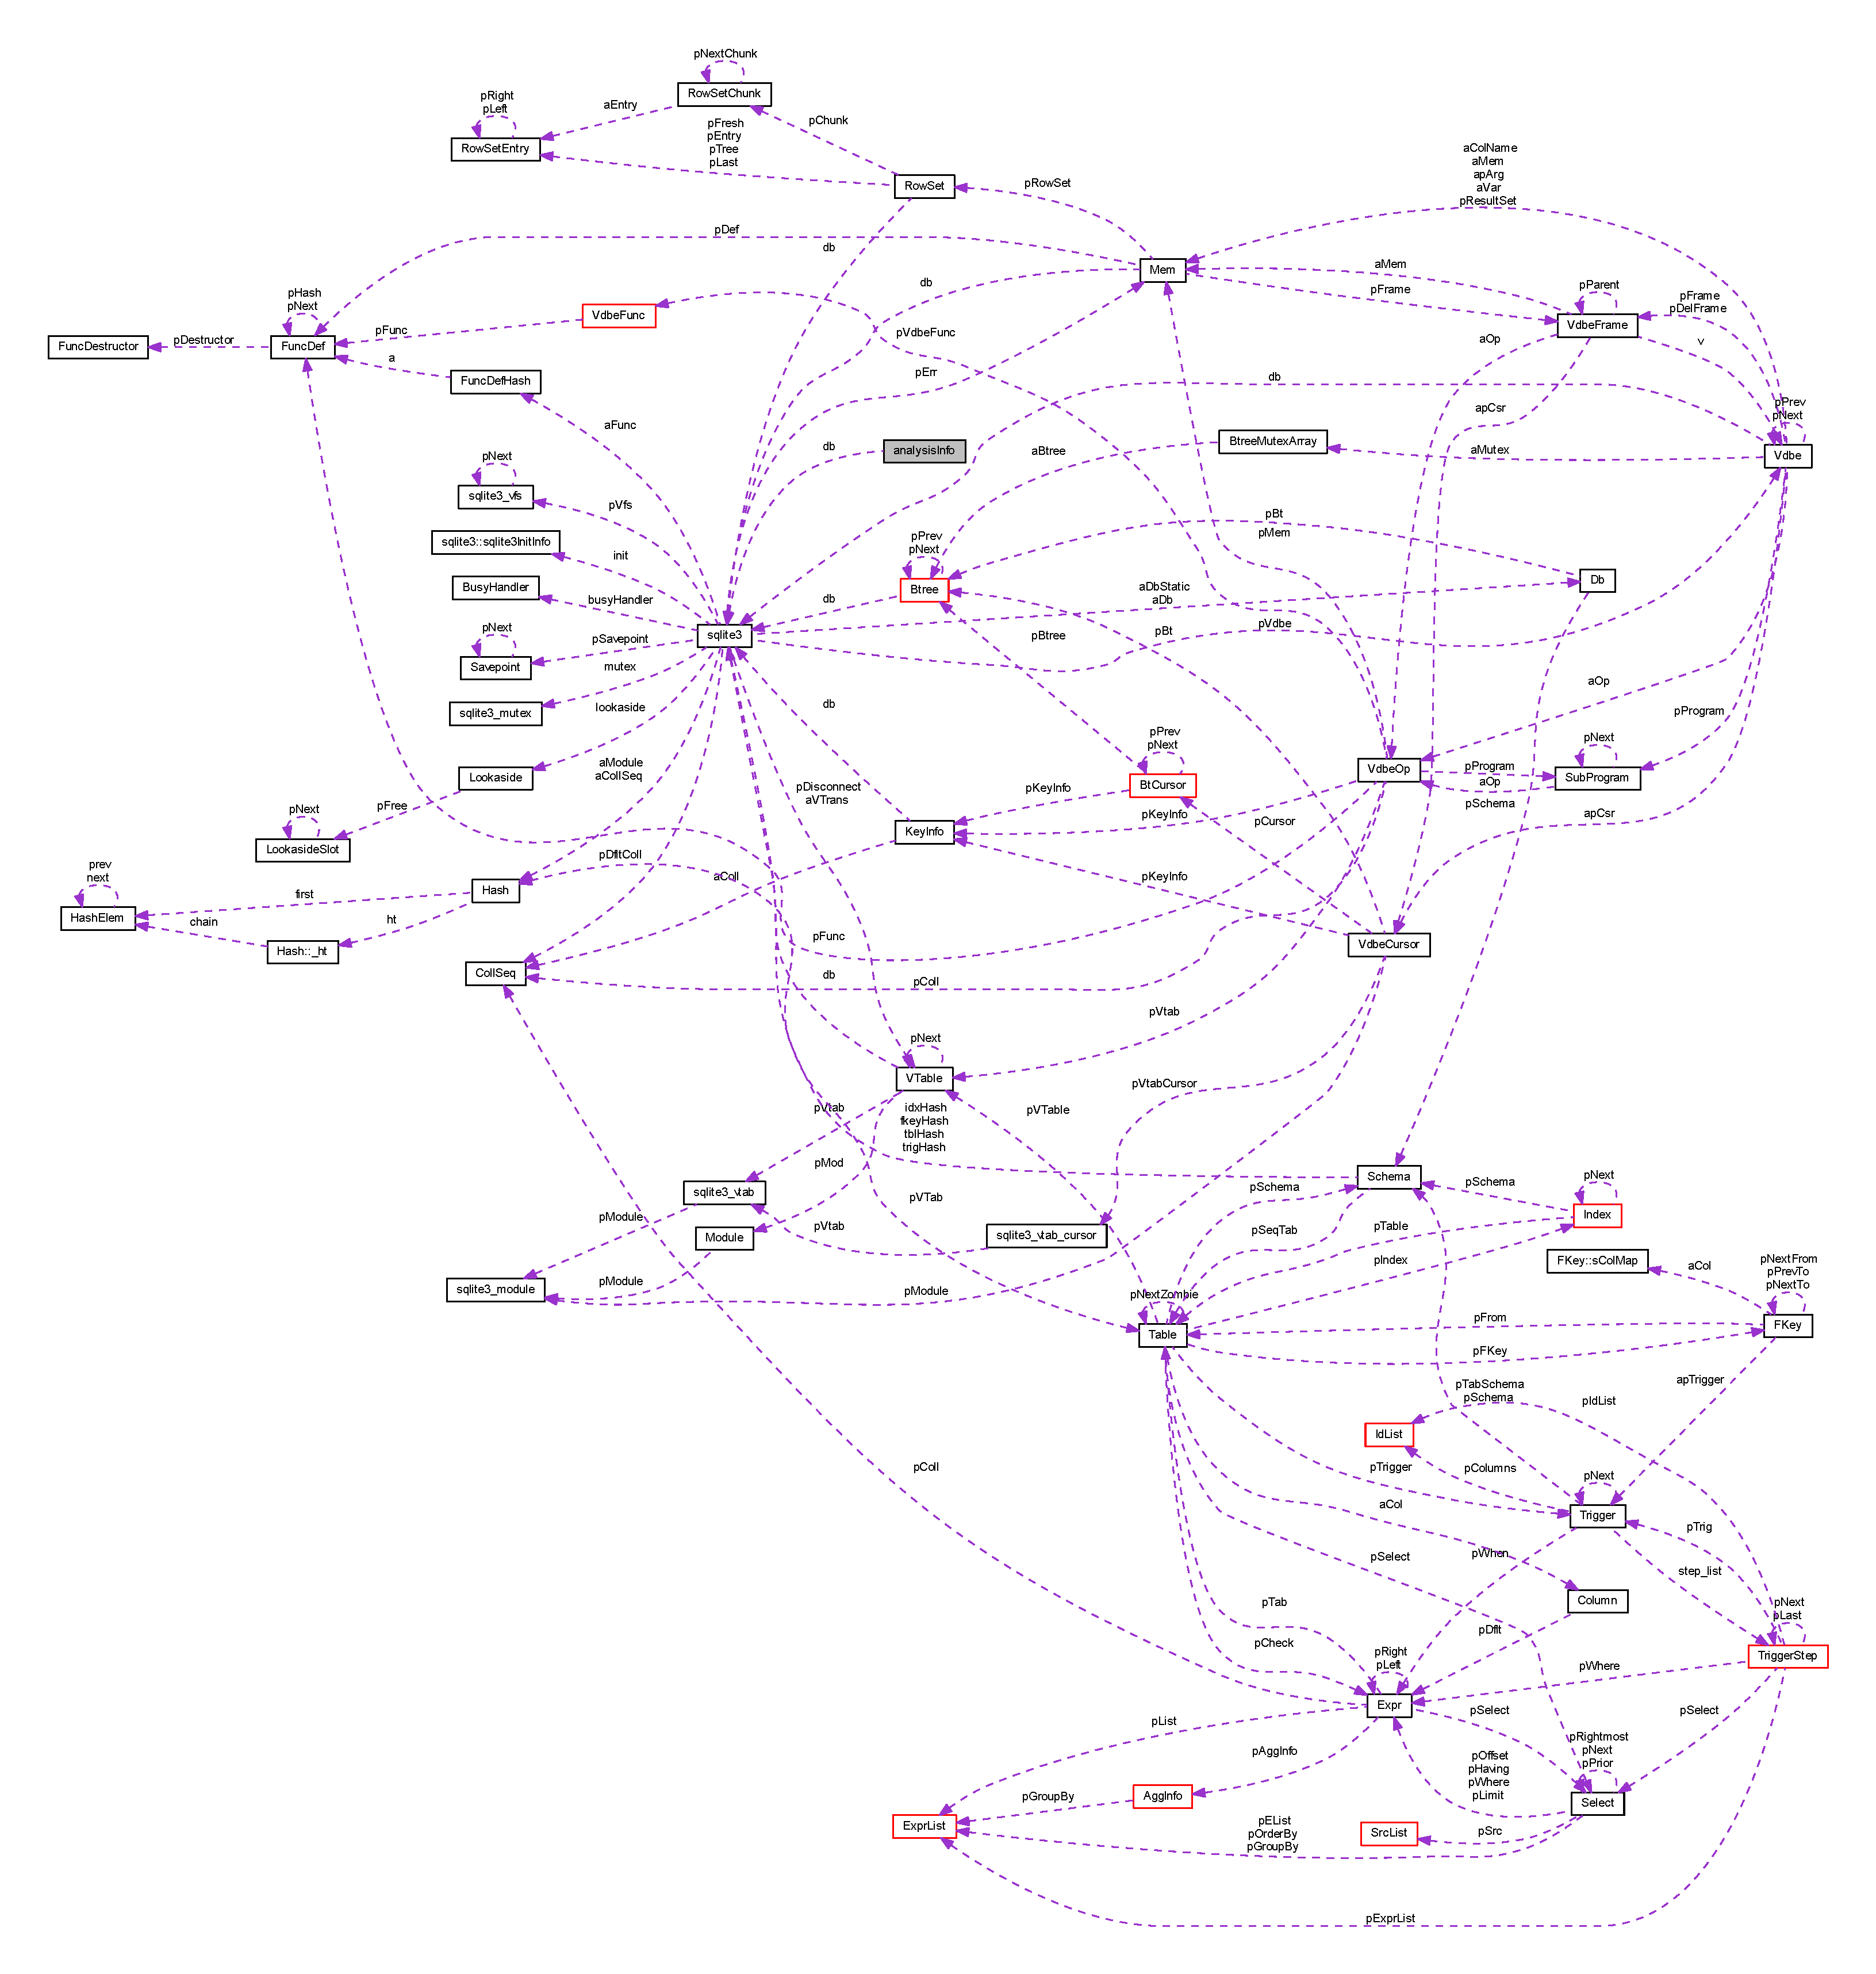
\includegraphics[width=350pt]{structanalysis_info__coll__graph}
\end{center}
\end{figure}
\subsection*{Public Attributes}
\begin{DoxyCompactItemize}
\item 
\hypertarget{structanalysis_info_a13108eadc55ffe73a8825fb91cc0f9b5}{\hyperlink{structsqlite3}{sqlite3} $\ast$ {\bfseries db}}\label{structanalysis_info_a13108eadc55ffe73a8825fb91cc0f9b5}

\item 
\hypertarget{structanalysis_info_accbe3c1f5613ffa13b9578e58a5d850a}{const char $\ast$ {\bfseries z\-Database}}\label{structanalysis_info_accbe3c1f5613ffa13b9578e58a5d850a}

\end{DoxyCompactItemize}


The documentation for this struct was generated from the following file\-:\begin{DoxyCompactItemize}
\item 
C\-:/\-Users/\-Vitor/\-Desktop/\-Work\-Space/\-P\-R\-O\-J\-E\-T\-O\-\_\-\-F\-I\-N\-A\-L\-\_\-\-P\-O\-O/\-P\-R\-O\-J\-E\-T\-O\-\_\-\-D\-E\-V/\-P\-R\-O\-J\-E\-T\-O/\-Projeto\-\_\-codeblocks/sqlite3.\-c\end{DoxyCompactItemize}

\hypertarget{struct_attach_key}{\section{Attach\-Key Struct Reference}
\label{struct_attach_key}\index{Attach\-Key@{Attach\-Key}}
}


Collaboration diagram for Attach\-Key\-:\nopagebreak
\begin{figure}[H]
\begin{center}
\leavevmode
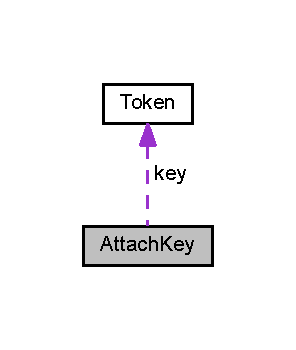
\includegraphics[width=142pt]{struct_attach_key__coll__graph}
\end{center}
\end{figure}
\subsection*{Public Attributes}
\begin{DoxyCompactItemize}
\item 
\hypertarget{struct_attach_key_acd780bfae7415a79a90fa5ceb41515cd}{int {\bfseries type}}\label{struct_attach_key_acd780bfae7415a79a90fa5ceb41515cd}

\item 
\hypertarget{struct_attach_key_a267449f11a142a3b88c54aa01f842ad0}{\hyperlink{struct_token}{Token} {\bfseries key}}\label{struct_attach_key_a267449f11a142a3b88c54aa01f842ad0}

\end{DoxyCompactItemize}


The documentation for this struct was generated from the following file\-:\begin{DoxyCompactItemize}
\item 
C\-:/\-Users/\-Vitor/\-Desktop/\-Work\-Space/\-P\-R\-O\-J\-E\-T\-O\-\_\-\-F\-I\-N\-A\-L\-\_\-\-P\-O\-O/\-P\-R\-O\-J\-E\-T\-O\-\_\-\-D\-E\-V/\-P\-R\-O\-J\-E\-T\-O/\-Projeto\-\_\-codeblocks/sqlite3.\-c\end{DoxyCompactItemize}

\hypertarget{struct_auth_context}{\section{Auth\-Context Struct Reference}
\label{struct_auth_context}\index{Auth\-Context@{Auth\-Context}}
}


Collaboration diagram for Auth\-Context\-:\nopagebreak
\begin{figure}[H]
\begin{center}
\leavevmode
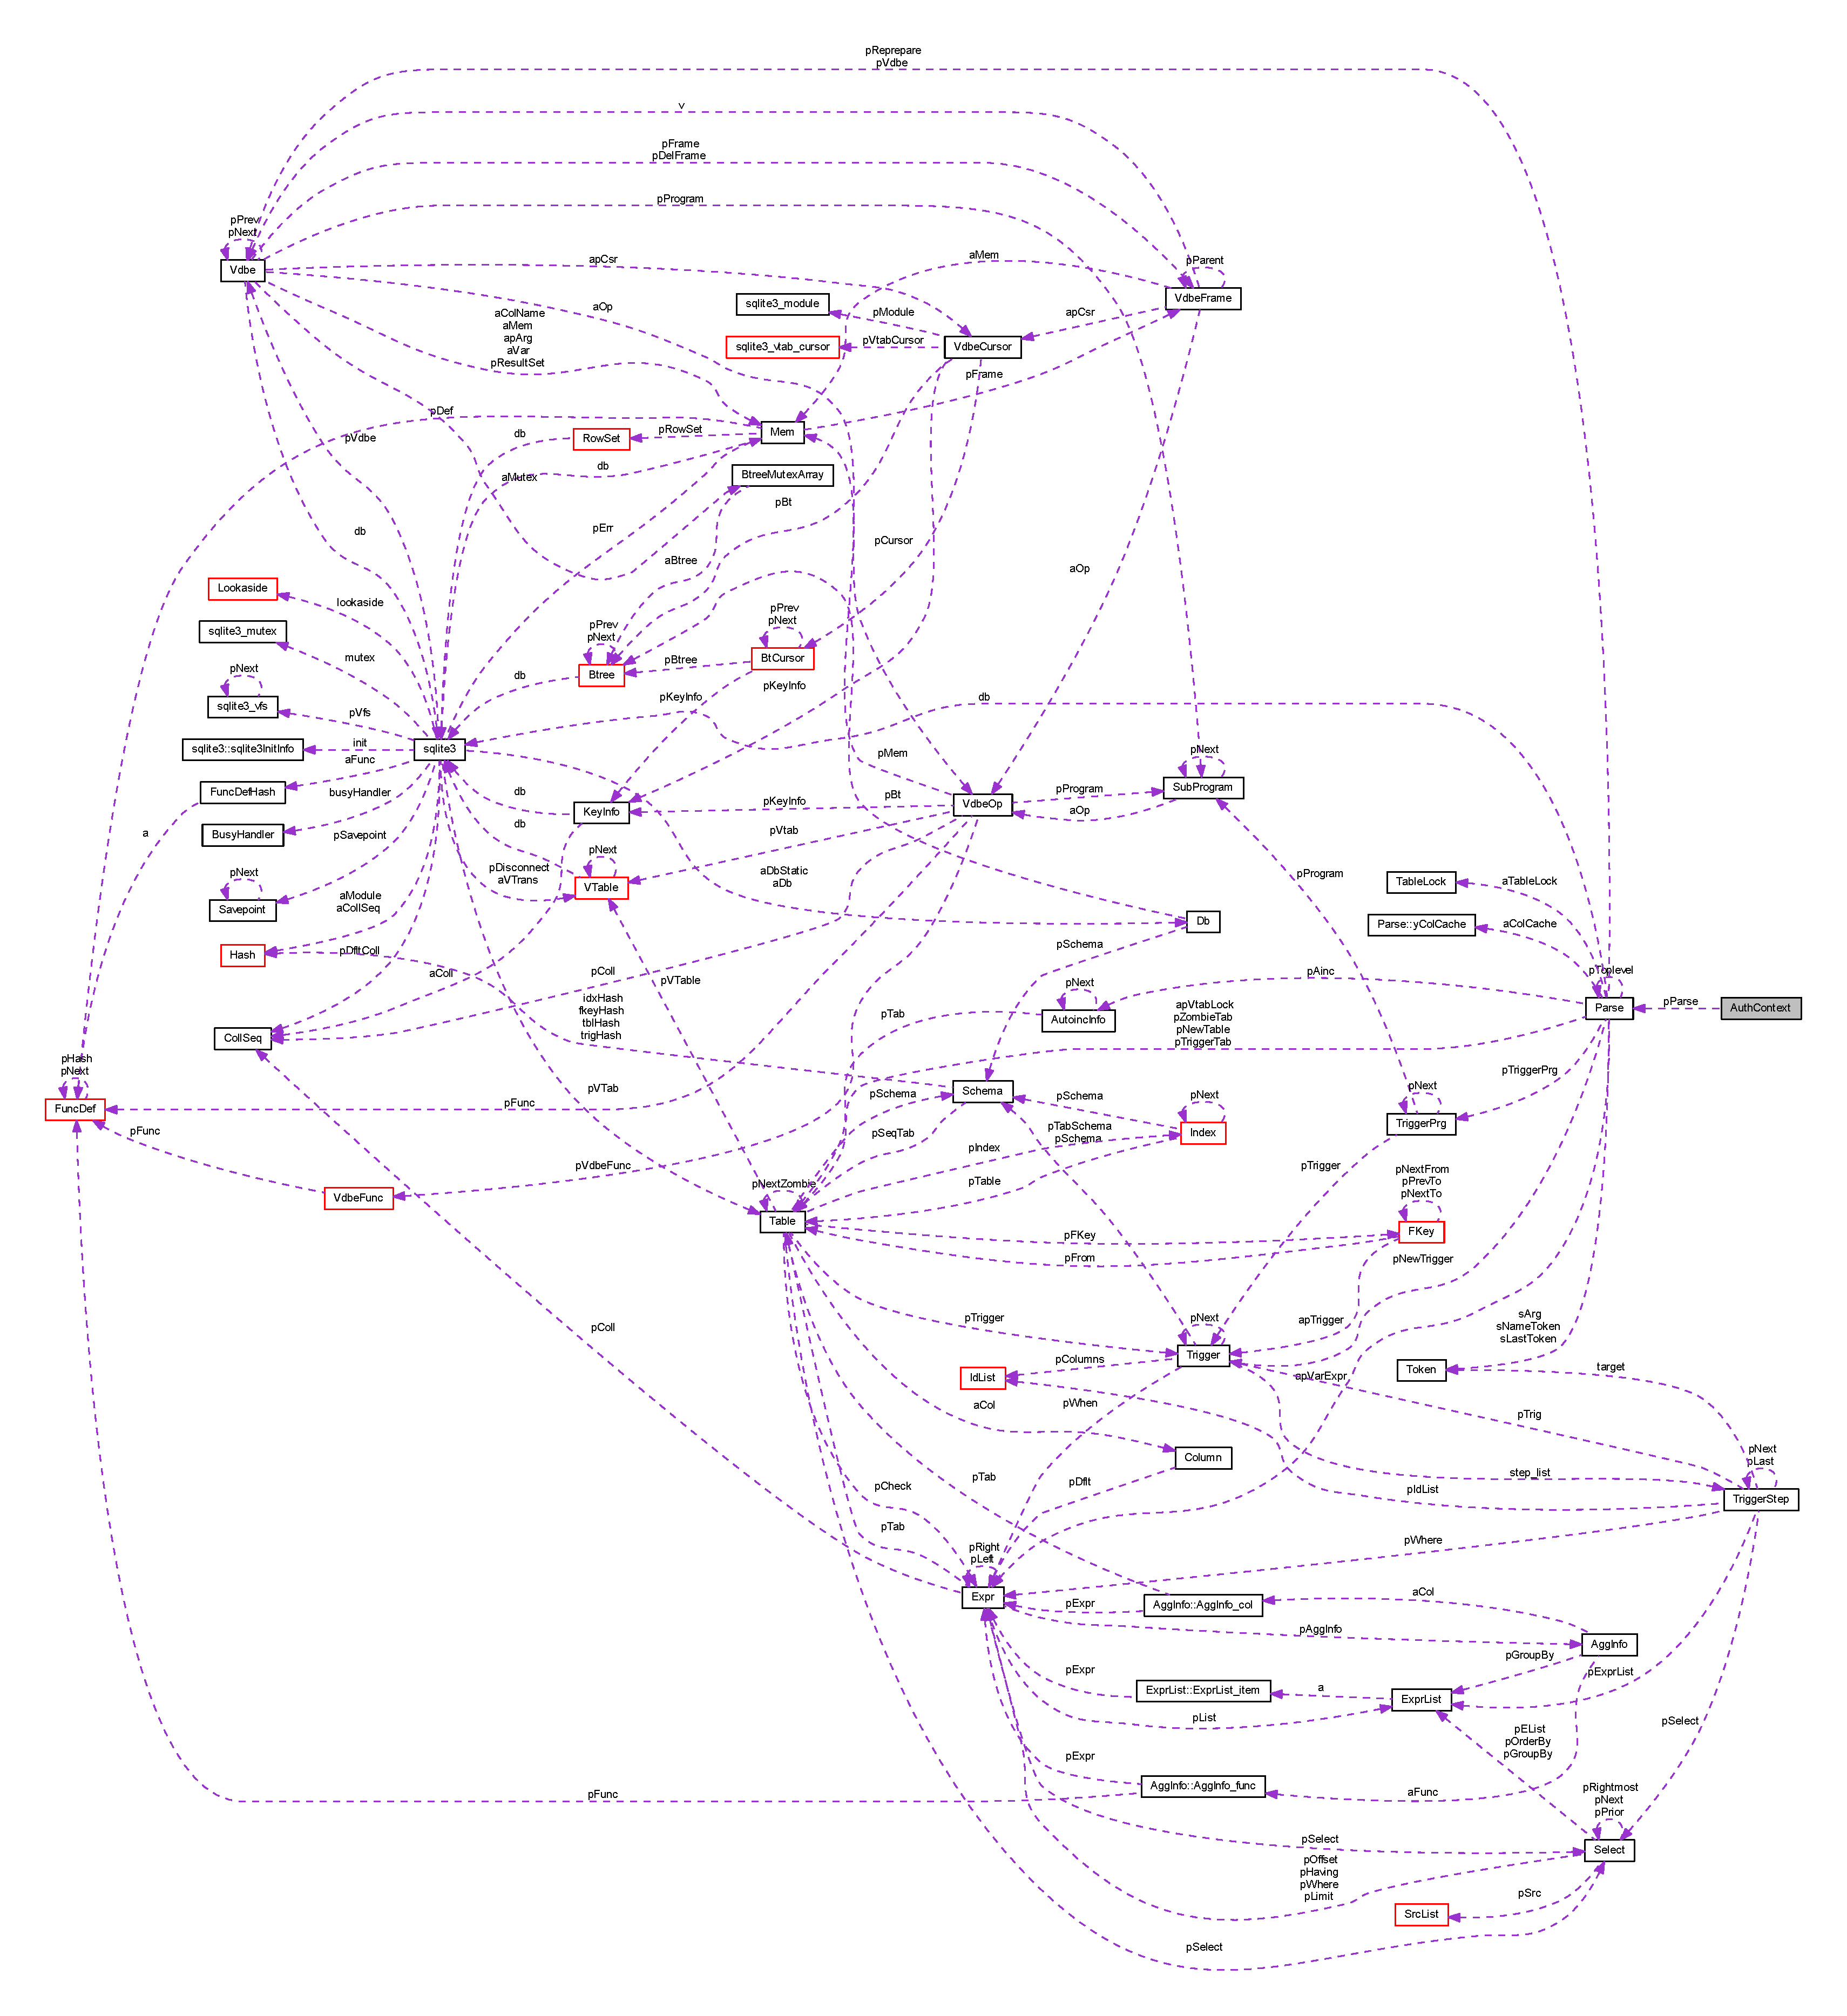
\includegraphics[width=350pt]{struct_auth_context__coll__graph}
\end{center}
\end{figure}
\subsection*{Public Attributes}
\begin{DoxyCompactItemize}
\item 
\hypertarget{struct_auth_context_a1b095b152b72326476ac3f7edcaee78a}{const char $\ast$ {\bfseries z\-Auth\-Context}}\label{struct_auth_context_a1b095b152b72326476ac3f7edcaee78a}

\item 
\hypertarget{struct_auth_context_a8df2931d8f4facf59073c92315b00bfa}{\hyperlink{struct_parse}{Parse} $\ast$ {\bfseries p\-Parse}}\label{struct_auth_context_a8df2931d8f4facf59073c92315b00bfa}

\end{DoxyCompactItemize}


The documentation for this struct was generated from the following file\-:\begin{DoxyCompactItemize}
\item 
C\-:/\-Users/\-Vitor/\-Desktop/\-Work\-Space/\-P\-R\-O\-J\-E\-T\-O\-\_\-\-F\-I\-N\-A\-L\-\_\-\-P\-O\-O/\-P\-R\-O\-J\-E\-T\-O\-\_\-\-D\-E\-V/\-P\-R\-O\-J\-E\-T\-O/\-Projeto\-\_\-codeblocks/sqlite3.\-c\end{DoxyCompactItemize}

\hypertarget{struct_autoinc_info}{\section{Autoinc\-Info Struct Reference}
\label{struct_autoinc_info}\index{Autoinc\-Info@{Autoinc\-Info}}
}


Collaboration diagram for Autoinc\-Info\-:\nopagebreak
\begin{figure}[H]
\begin{center}
\leavevmode
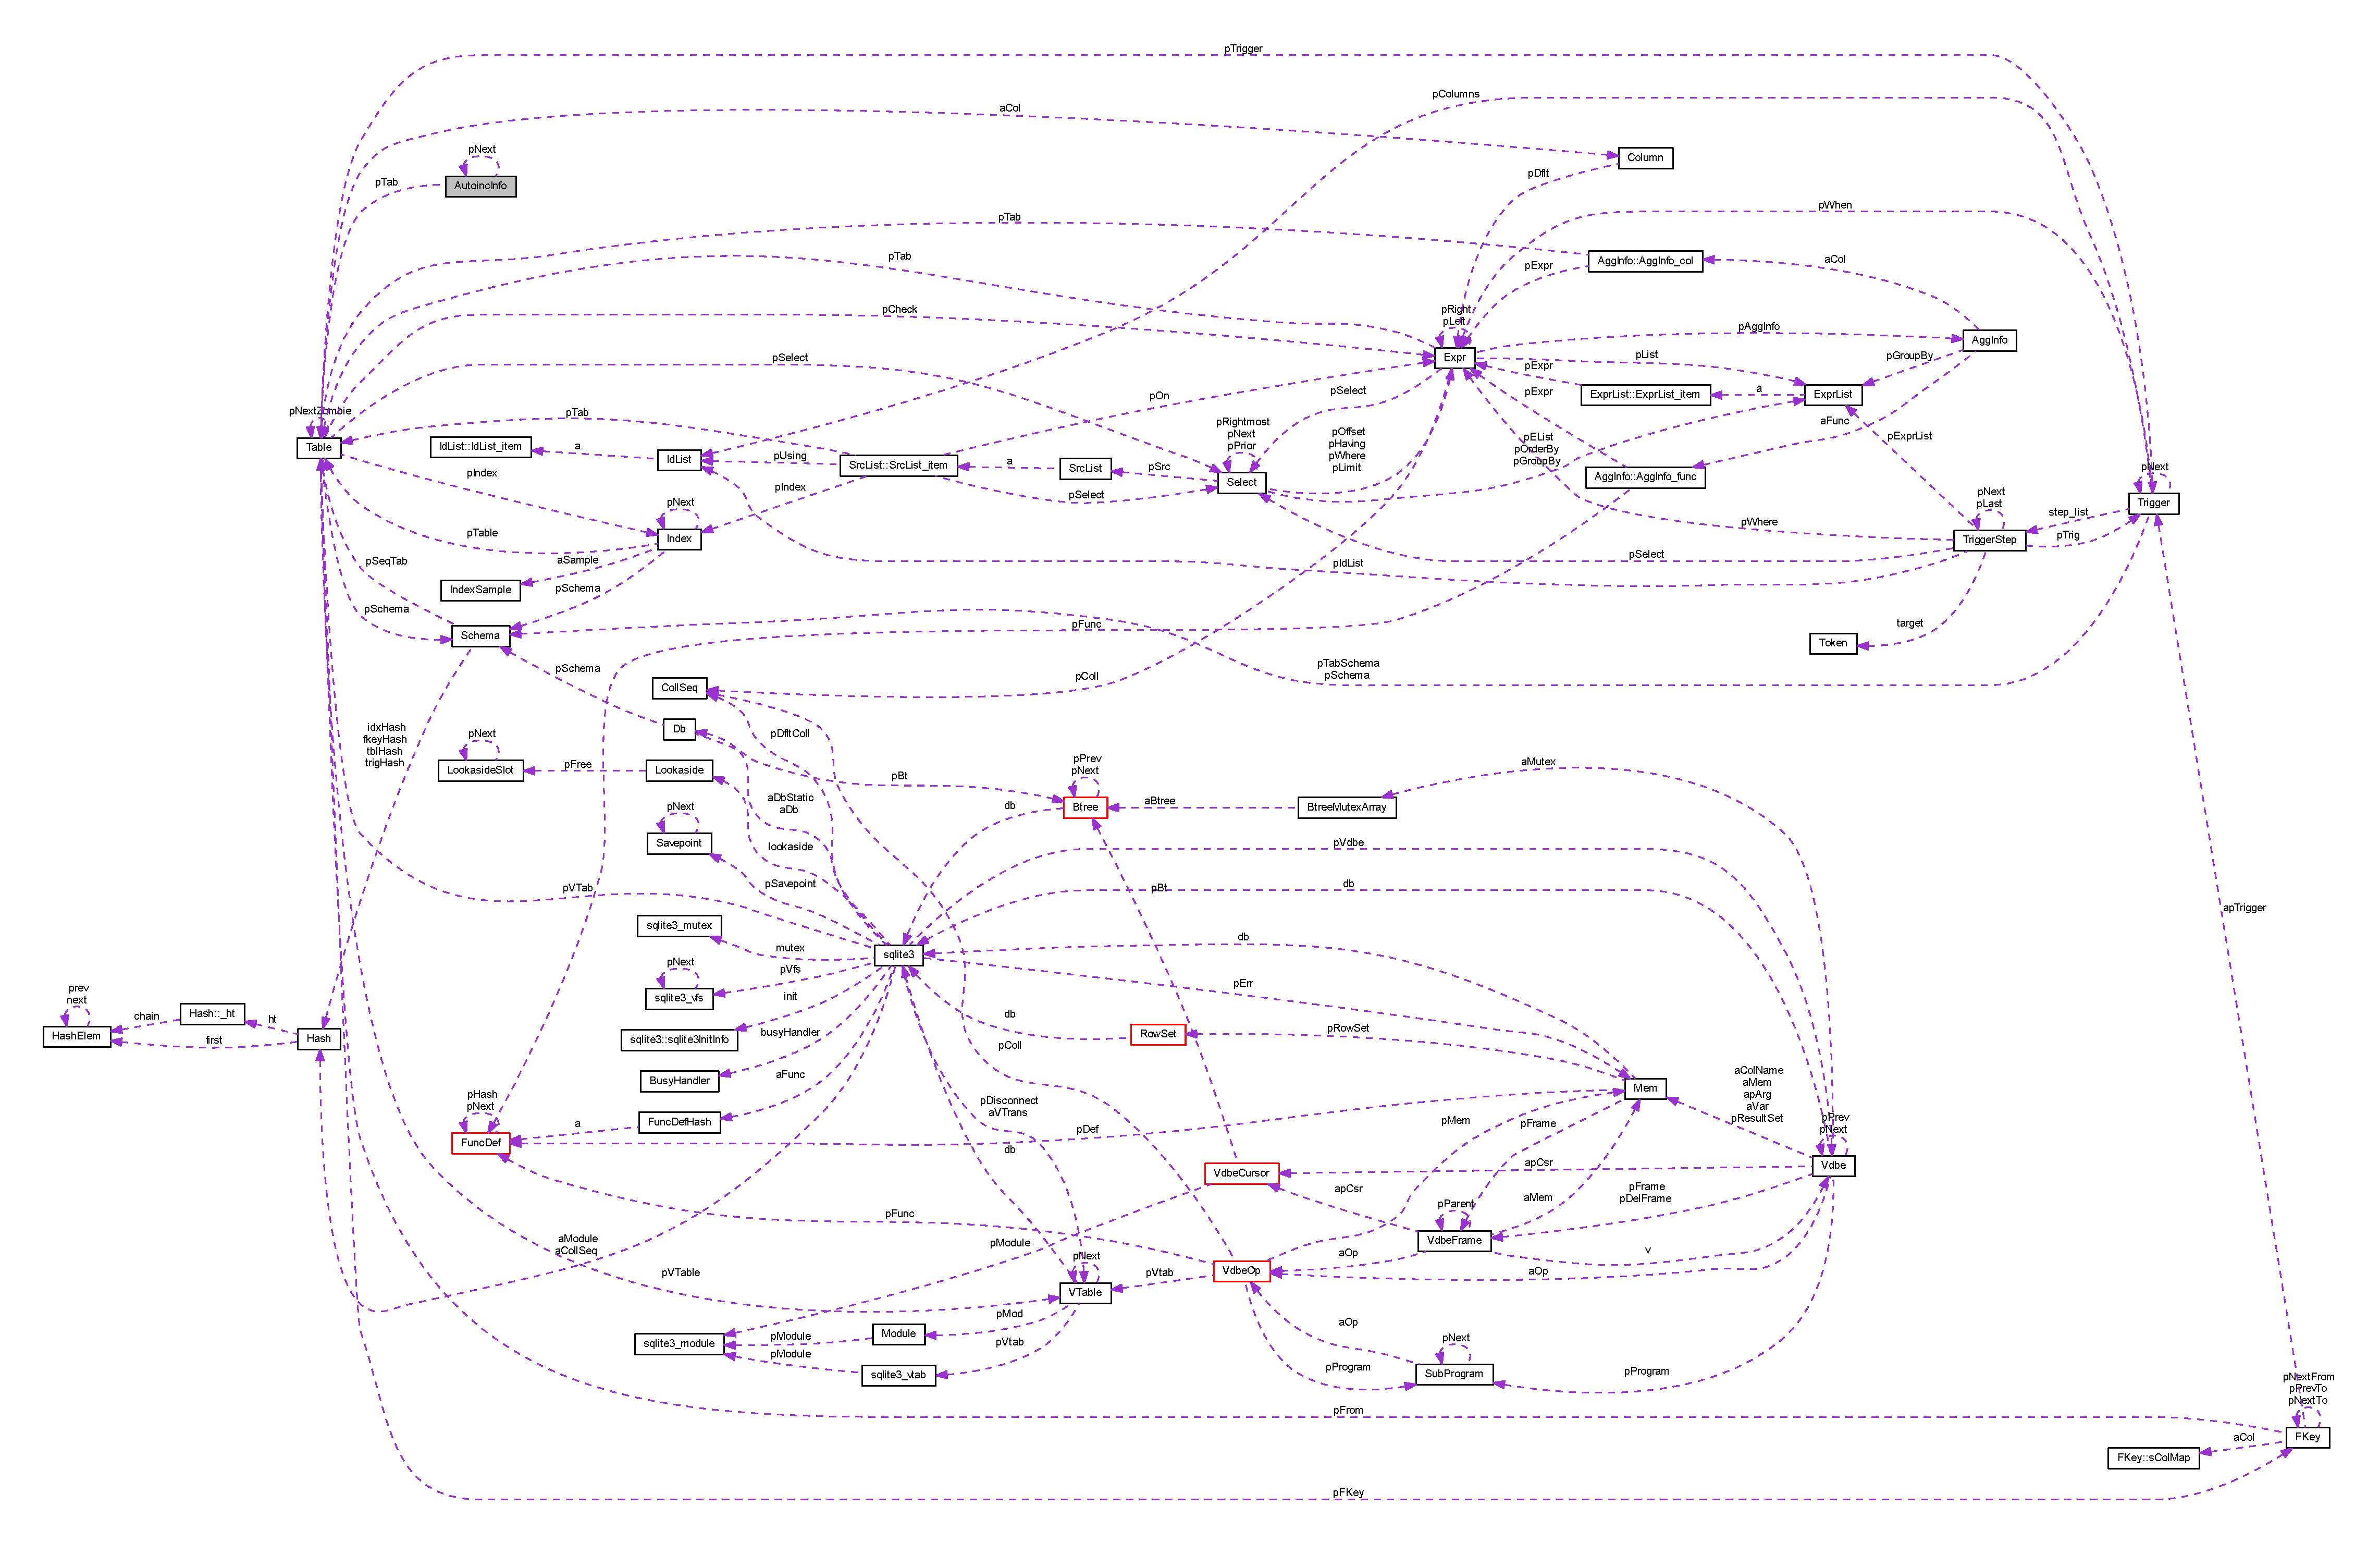
\includegraphics[width=350pt]{struct_autoinc_info__coll__graph}
\end{center}
\end{figure}
\subsection*{Public Attributes}
\begin{DoxyCompactItemize}
\item 
\hypertarget{struct_autoinc_info_aa77fb076beea013c25df4e49dba4b6f6}{\hyperlink{struct_autoinc_info}{Autoinc\-Info} $\ast$ {\bfseries p\-Next}}\label{struct_autoinc_info_aa77fb076beea013c25df4e49dba4b6f6}

\item 
\hypertarget{struct_autoinc_info_a0cf785b0cbaddb4215a8408f8e13075e}{\hyperlink{struct_table}{Table} $\ast$ {\bfseries p\-Tab}}\label{struct_autoinc_info_a0cf785b0cbaddb4215a8408f8e13075e}

\item 
\hypertarget{struct_autoinc_info_ae7234e0916b11ef97377bdfd6c7c4568}{int {\bfseries i\-Db}}\label{struct_autoinc_info_ae7234e0916b11ef97377bdfd6c7c4568}

\item 
\hypertarget{struct_autoinc_info_af180977ee7dcc8cab862185692f57cc5}{int {\bfseries reg\-Ctr}}\label{struct_autoinc_info_af180977ee7dcc8cab862185692f57cc5}

\end{DoxyCompactItemize}


The documentation for this struct was generated from the following file\-:\begin{DoxyCompactItemize}
\item 
C\-:/\-Users/\-Vitor/\-Desktop/\-Work\-Space/\-P\-R\-O\-J\-E\-T\-O\-\_\-\-F\-I\-N\-A\-L\-\_\-\-P\-O\-O/\-P\-R\-O\-J\-E\-T\-O\-\_\-\-D\-E\-V/\-P\-R\-O\-J\-E\-T\-O/\-Projeto\-\_\-codeblocks/sqlite3.\-c\end{DoxyCompactItemize}

\hypertarget{struct_vdbe_func_1_1_aux_data}{\section{Vdbe\-Func\-:\-:Aux\-Data Struct Reference}
\label{struct_vdbe_func_1_1_aux_data}\index{Vdbe\-Func\-::\-Aux\-Data@{Vdbe\-Func\-::\-Aux\-Data}}
}
\subsection*{Public Attributes}
\begin{DoxyCompactItemize}
\item 
\hypertarget{struct_vdbe_func_1_1_aux_data_ad2ceeac1dec76bbb661f6418ec582539}{void $\ast$ {\bfseries p\-Aux}}\label{struct_vdbe_func_1_1_aux_data_ad2ceeac1dec76bbb661f6418ec582539}

\item 
\hypertarget{struct_vdbe_func_1_1_aux_data_a6742f89d0634b5fc6684f245bac76fd5}{void($\ast$ {\bfseries x\-Delete} )(void $\ast$)}\label{struct_vdbe_func_1_1_aux_data_a6742f89d0634b5fc6684f245bac76fd5}

\end{DoxyCompactItemize}


The documentation for this struct was generated from the following file\-:\begin{DoxyCompactItemize}
\item 
sqlite3.\-c\end{DoxyCompactItemize}

\hypertarget{class_basic_type}{\section{Basic\-Type Class Reference}
\label{class_basic_type}\index{Basic\-Type@{Basic\-Type}}
}


Essa e a classe responsavel por ser um padrao de classe para clases tipos basicos \par
 tendo os metodos obrigratorios para todas essas e os mentodos mais gerais ja implemtados\par
 inline garantindo uma economia de memoria.  




{\ttfamily \#include $<$Tipos\-Basicos.\-h$>$}



Inheritance diagram for Basic\-Type\-:\nopagebreak
\begin{figure}[H]
\begin{center}
\leavevmode
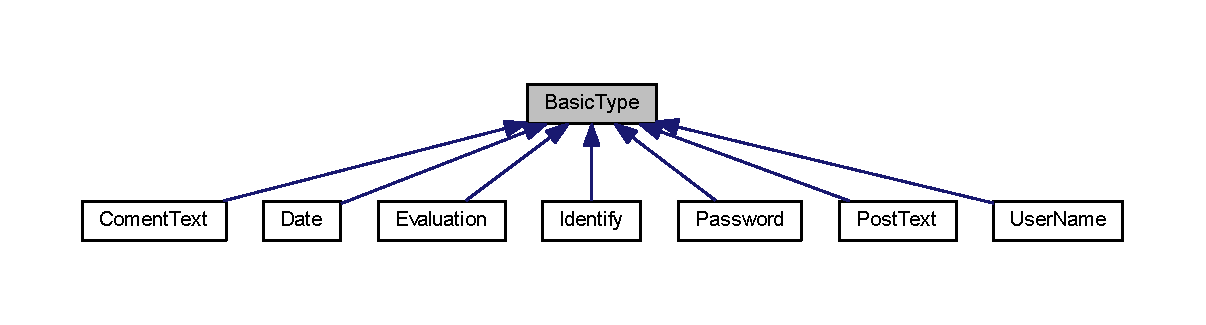
\includegraphics[width=350pt]{class_basic_type__inherit__graph}
\end{center}
\end{figure}
\subsection*{Public Member Functions}
\begin{DoxyCompactItemize}
\item 
void \hyperlink{class_basic_type_a94da6e04e150bbfc35072df5897e8e21}{set\-Value} (const string \&\hyperlink{class_basic_type_af9b2c5cc32647df01083a6802e913dbf}{value})  throw (invalid\-\_\-argument)
\begin{DoxyCompactList}\small\item\em Da set no valor do compo nome do usuario. \end{DoxyCompactList}\item 
string \hyperlink{class_basic_type_af0b6be797220a64bc975744cd65c93ab}{get\-Value} () const 
\begin{DoxyCompactList}\small\item\em Pega o valor armazendo value. \end{DoxyCompactList}\end{DoxyCompactItemize}
\subsection*{Protected Member Functions}
\begin{DoxyCompactItemize}
\item 
virtual void \hyperlink{class_basic_type_a0990f4e2537208845f85f0f8f638123b}{validate} (const string \&\hyperlink{class_basic_type_af9b2c5cc32647df01083a6802e913dbf}{value})=0  throw (invalid\-\_\-argument)
\begin{DoxyCompactList}\small\item\em Validar os argumentos antes que estes sejam setados nas classes. \end{DoxyCompactList}\end{DoxyCompactItemize}
\subsection*{Protected Attributes}
\begin{DoxyCompactItemize}
\item 
string \hyperlink{class_basic_type_af9b2c5cc32647df01083a6802e913dbf}{value}
\end{DoxyCompactItemize}


\subsection{Detailed Description}
Essa e a classe responsavel por ser um padrao de classe para clases tipos basicos \par
 tendo os metodos obrigratorios para todas essas e os mentodos mais gerais ja implemtados\par
 inline garantindo uma economia de memoria. 

\subsection{Member Function Documentation}
\hypertarget{class_basic_type_af0b6be797220a64bc975744cd65c93ab}{\index{Basic\-Type@{Basic\-Type}!get\-Value@{get\-Value}}
\index{get\-Value@{get\-Value}!BasicType@{Basic\-Type}}
\subsubsection[{get\-Value}]{\setlength{\rightskip}{0pt plus 5cm}string Basic\-Type\-::get\-Value (
\begin{DoxyParamCaption}
{}
\end{DoxyParamCaption}
) const\hspace{0.3cm}{\ttfamily [inline]}}}\label{class_basic_type_af0b6be797220a64bc975744cd65c93ab}


Pega o valor armazendo value. 

\begin{DoxyReturn}{Returns}
O o string que pode variar de conteudo a partir de que classe se usa. 
\end{DoxyReturn}


Here is the caller graph for this function\-:\nopagebreak
\begin{figure}[H]
\begin{center}
\leavevmode
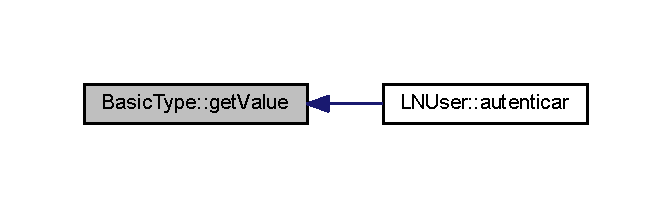
\includegraphics[width=322pt]{class_basic_type_af0b6be797220a64bc975744cd65c93ab_icgraph}
\end{center}
\end{figure}


\hypertarget{class_basic_type_a94da6e04e150bbfc35072df5897e8e21}{\index{Basic\-Type@{Basic\-Type}!set\-Value@{set\-Value}}
\index{set\-Value@{set\-Value}!BasicType@{Basic\-Type}}
\subsubsection[{set\-Value}]{\setlength{\rightskip}{0pt plus 5cm}void Basic\-Type\-::set\-Value (
\begin{DoxyParamCaption}
\item[{const string \&}]{value}
\end{DoxyParamCaption}
)  throw (invalid\-\_\-argument)\hspace{0.3cm}{\ttfamily [inline]}}}\label{class_basic_type_a94da6e04e150bbfc35072df5897e8e21}


Da set no valor do compo nome do usuario. 


\begin{DoxyParams}{Parameters}
{\em value} & \-: o nome do Usuario. \\
\hline
\end{DoxyParams}

\begin{DoxyExceptions}{Exceptions}
{\em std\-::invalid\-\_\-argument} & o argumeto e invalido \\
\hline
\end{DoxyExceptions}


Here is the caller graph for this function\-:\nopagebreak
\begin{figure}[H]
\begin{center}
\leavevmode
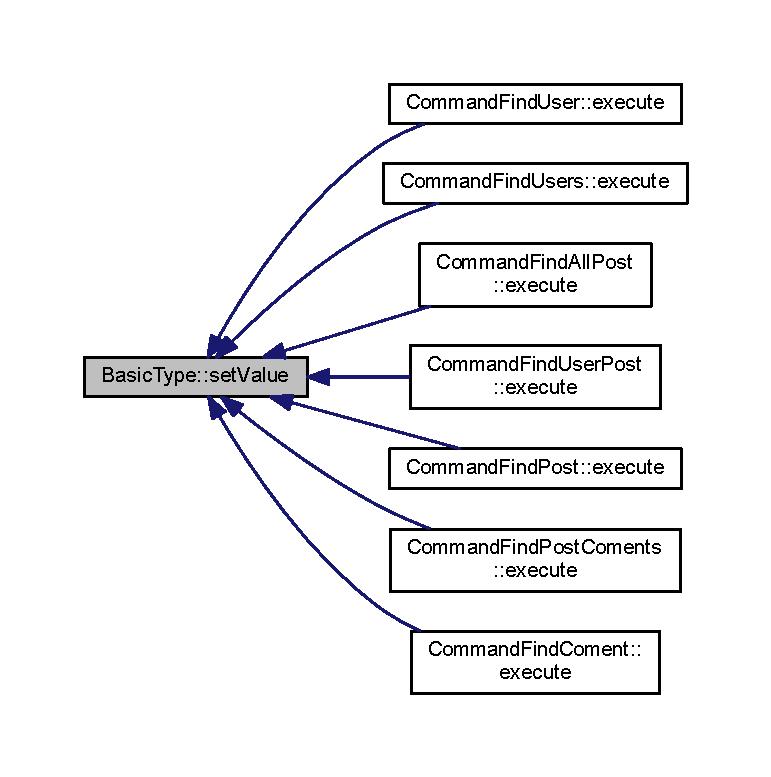
\includegraphics[width=350pt]{class_basic_type_a94da6e04e150bbfc35072df5897e8e21_icgraph}
\end{center}
\end{figure}


\hypertarget{class_basic_type_a0990f4e2537208845f85f0f8f638123b}{\index{Basic\-Type@{Basic\-Type}!validate@{validate}}
\index{validate@{validate}!BasicType@{Basic\-Type}}
\subsubsection[{validate}]{\setlength{\rightskip}{0pt plus 5cm}void Basic\-Type\-::validate (
\begin{DoxyParamCaption}
\item[{const string \&}]{value}
\end{DoxyParamCaption}
)  throw (invalid\-\_\-argument)\hspace{0.3cm}{\ttfamily [protected]}, {\ttfamily [pure virtual]}}}\label{class_basic_type_a0990f4e2537208845f85f0f8f638123b}


Validar os argumentos antes que estes sejam setados nas classes. 


\begin{DoxyParams}{Parameters}
{\em value} & \-: e o valor a ser validado \\
\hline
\end{DoxyParams}

\begin{DoxyExceptions}{Exceptions}
{\em std\-::invalid\-\_\-argument} & o argumeto e invalido \\
\hline
\end{DoxyExceptions}


\subsection{Member Data Documentation}
\hypertarget{class_basic_type_af9b2c5cc32647df01083a6802e913dbf}{\index{Basic\-Type@{Basic\-Type}!value@{value}}
\index{value@{value}!BasicType@{Basic\-Type}}
\subsubsection[{value}]{\setlength{\rightskip}{0pt plus 5cm}string Basic\-Type\-::value\hspace{0.3cm}{\ttfamily [protected]}}}\label{class_basic_type_af9b2c5cc32647df01083a6802e913dbf}
Esta string e usada para armazenar as informaçoes repassadas de cada classe apos a validaçao destas 

The documentation for this class was generated from the following file\-:\begin{DoxyCompactItemize}
\item 
C\-:/\-Users/\-Vitor/\-Desktop/\-Work\-Space/\-P\-R\-O\-J\-E\-T\-O\-\_\-\-F\-I\-N\-A\-L\-\_\-\-P\-O\-O/\-P\-R\-O\-J\-E\-T\-O\-\_\-\-D\-E\-V/\-P\-R\-O\-J\-E\-T\-O/\-Projeto\-\_\-codeblocks/\hyperlink{_tipos_basicos_8h}{Tipos\-Basicos.\-h}\end{DoxyCompactItemize}

\hypertarget{struct_bitvec}{\section{Bitvec Struct Reference}
\label{struct_bitvec}\index{Bitvec@{Bitvec}}
}


Collaboration diagram for Bitvec\-:\nopagebreak
\begin{figure}[H]
\begin{center}
\leavevmode
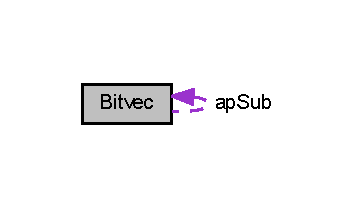
\includegraphics[width=171pt]{struct_bitvec__coll__graph}
\end{center}
\end{figure}
\subsection*{Public Attributes}
\begin{DoxyCompactItemize}
\item 
\hypertarget{struct_bitvec_ab36df8ece98aee080bae6de28c237de8}{u32 {\bfseries i\-Size}}\label{struct_bitvec_ab36df8ece98aee080bae6de28c237de8}

\item 
\hypertarget{struct_bitvec_ad6811debae9b972f2d94d667e994e3f6}{u32 {\bfseries n\-Set}}\label{struct_bitvec_ad6811debae9b972f2d94d667e994e3f6}

\item 
\hypertarget{struct_bitvec_a22cdb23eb424e07b6ce922de018a83d9}{u32 {\bfseries i\-Divisor}}\label{struct_bitvec_a22cdb23eb424e07b6ce922de018a83d9}

\item 
\hypertarget{struct_bitvec_a2ef3423696109b6b699aee3e736c4ed6}{\begin{tabbing}
xx\=xx\=xx\=xx\=xx\=xx\=xx\=xx\=xx\=\kill
union \{\\
\>BITVEC\_TELEM {\bfseries aBitmap} \mbox{[}BITVEC\_NELEM\mbox{]}\\
\>u32 {\bfseries aHash} \mbox{[}BITVEC\_NINT\mbox{]}\\
\>\hyperlink{struct_bitvec}{Bitvec} $\ast$ {\bfseries apSub} \mbox{[}BITVEC\_NPTR\mbox{]}\\
\} {\bfseries u}}\label{struct_bitvec_a2ef3423696109b6b699aee3e736c4ed6}
\\

\end{tabbing}\end{DoxyCompactItemize}


The documentation for this struct was generated from the following file\-:\begin{DoxyCompactItemize}
\item 
C\-:/\-Users/\-Vitor/\-Desktop/\-Work\-Space/\-P\-R\-O\-J\-E\-T\-O\-\_\-\-F\-I\-N\-A\-L\-\_\-\-P\-O\-O/\-P\-R\-O\-J\-E\-T\-O\-\_\-\-D\-E\-V/\-P\-R\-O\-J\-E\-T\-O/\-Projeto\-\_\-codeblocks/sqlite3.\-c\end{DoxyCompactItemize}

\hypertarget{struct_bt_cursor}{\section{Bt\-Cursor Struct Reference}
\label{struct_bt_cursor}\index{Bt\-Cursor@{Bt\-Cursor}}
}


Collaboration diagram for Bt\-Cursor\-:\nopagebreak
\begin{figure}[H]
\begin{center}
\leavevmode
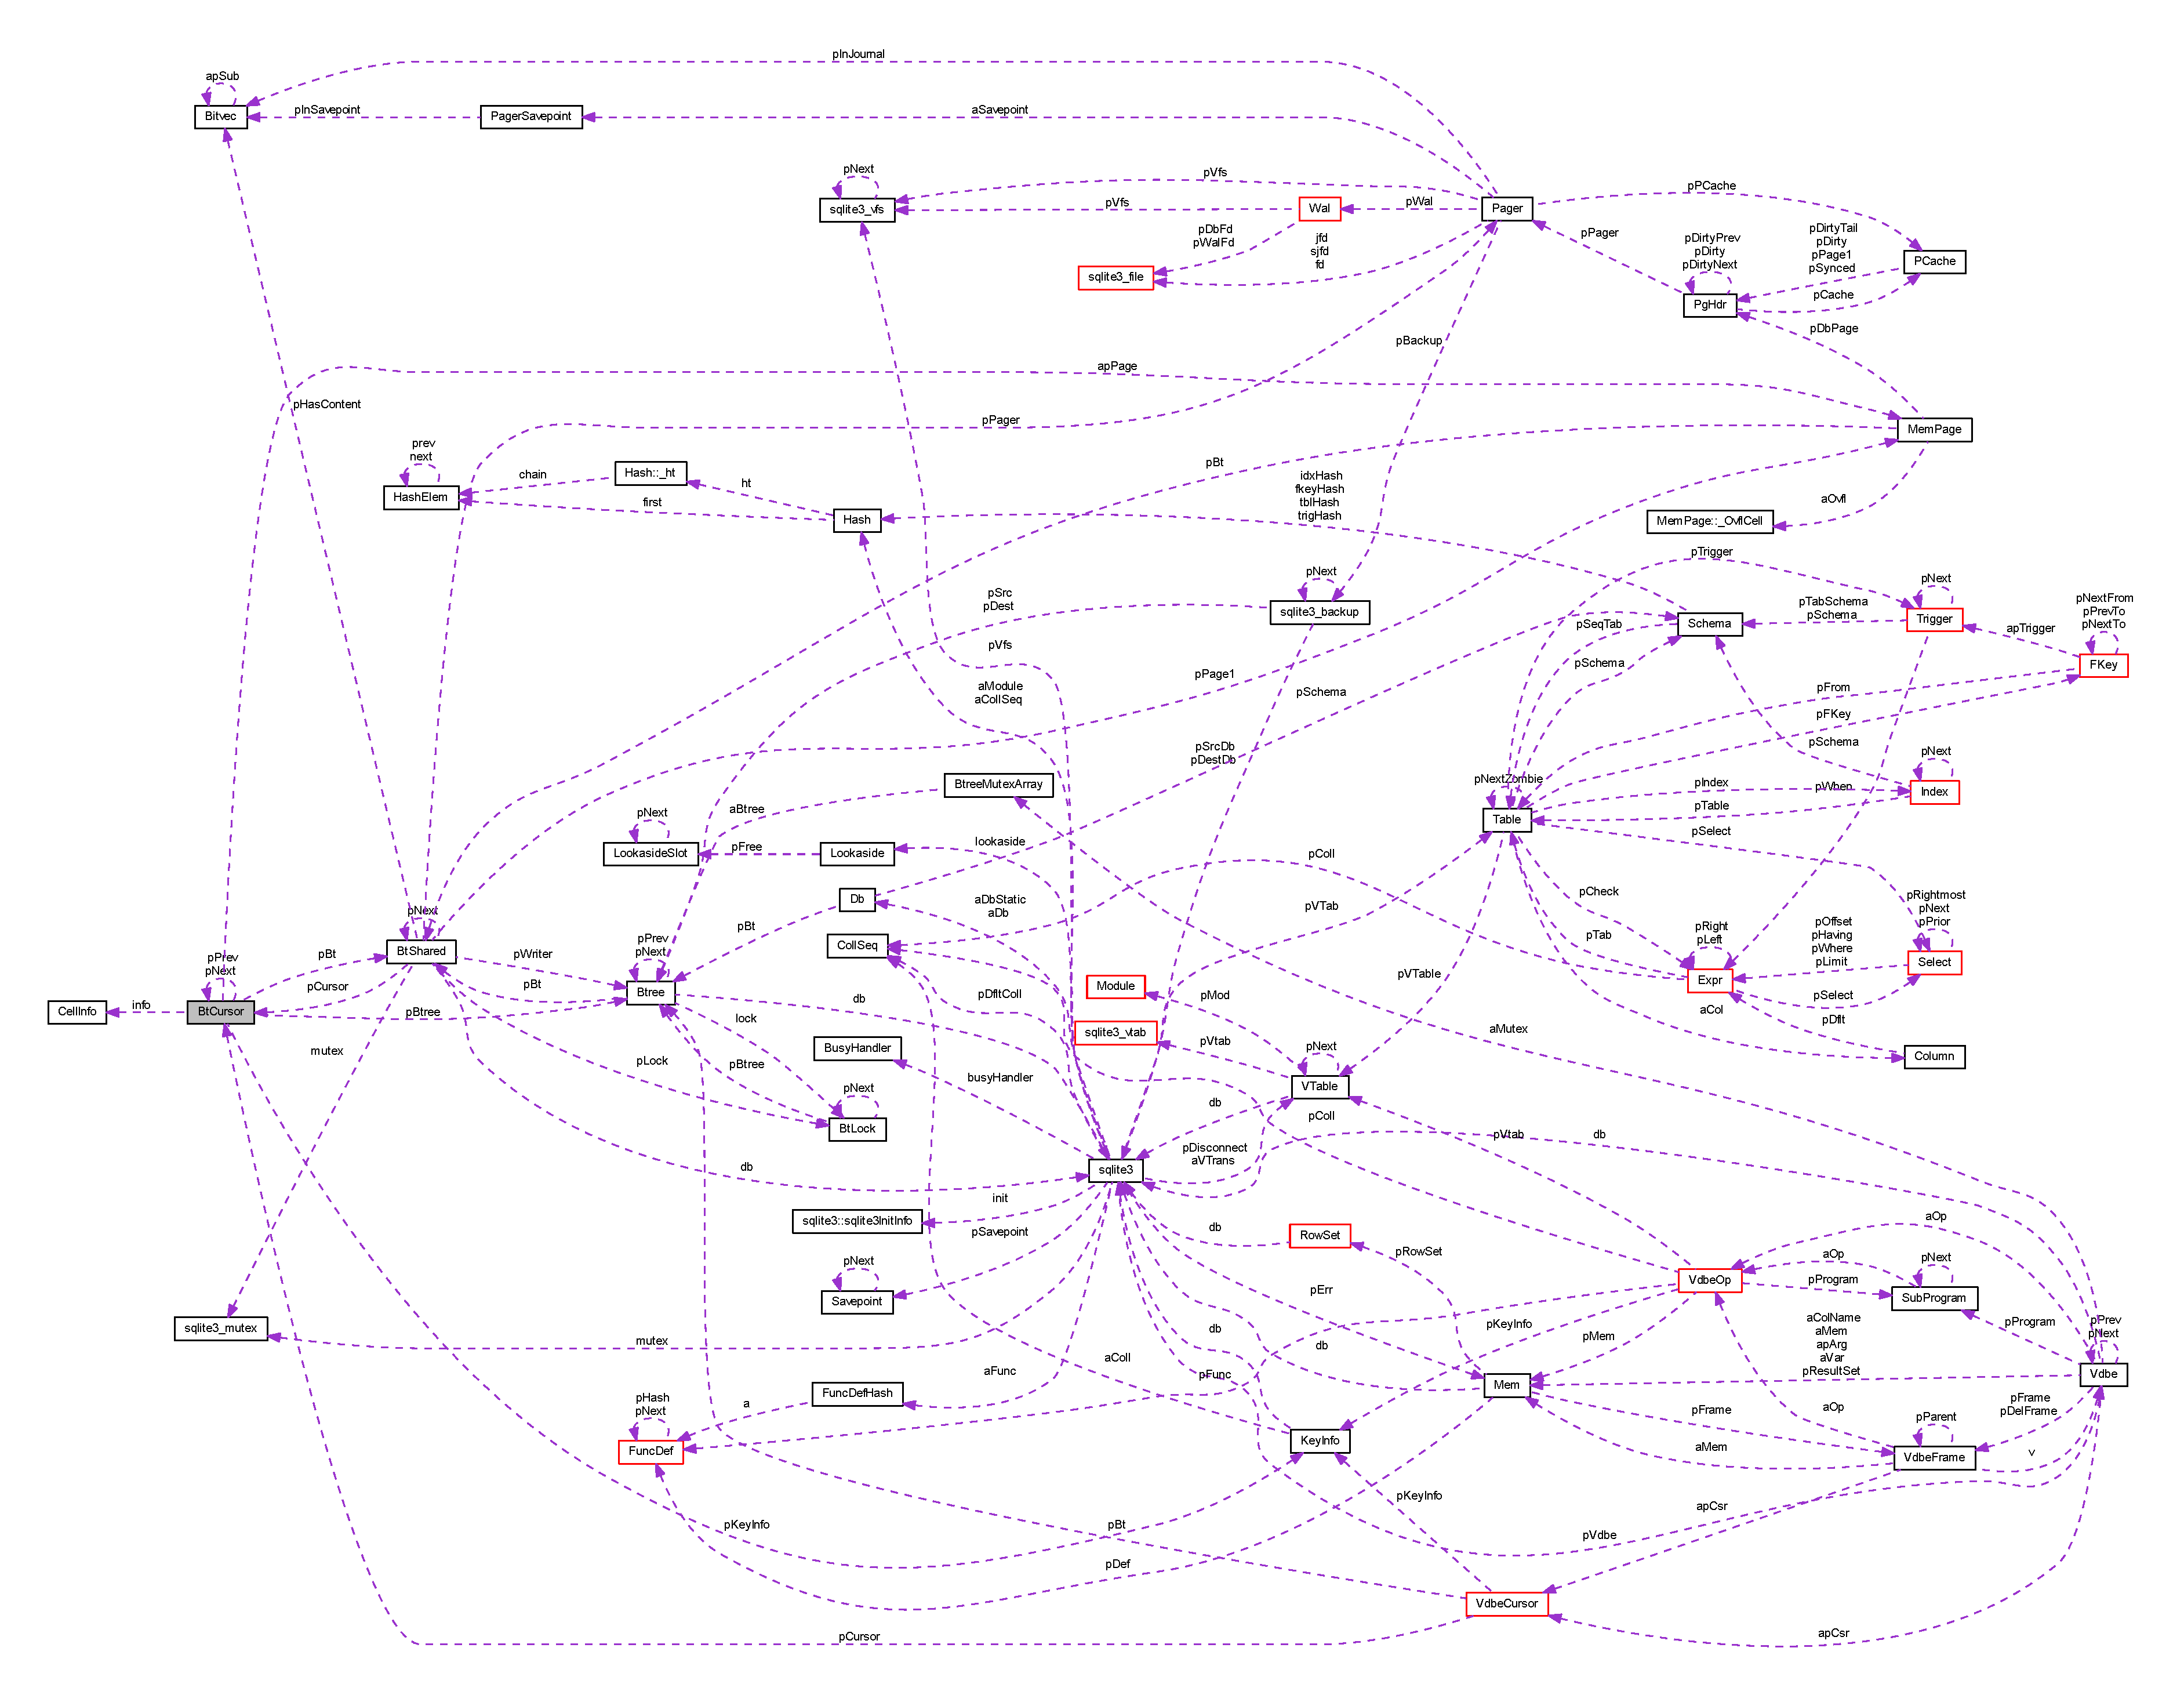
\includegraphics[width=350pt]{struct_bt_cursor__coll__graph}
\end{center}
\end{figure}
\subsection*{Public Attributes}
\begin{DoxyCompactItemize}
\item 
\hypertarget{struct_bt_cursor_a2ad810542eaf99c9919c585624bead6f}{\hyperlink{struct_btree}{Btree} $\ast$ {\bfseries p\-Btree}}\label{struct_bt_cursor_a2ad810542eaf99c9919c585624bead6f}

\item 
\hypertarget{struct_bt_cursor_a61c245712549192f7644e5ac23c00b74}{\hyperlink{struct_bt_shared}{Bt\-Shared} $\ast$ {\bfseries p\-Bt}}\label{struct_bt_cursor_a61c245712549192f7644e5ac23c00b74}

\item 
\hypertarget{struct_bt_cursor_ad2f8fe3aa7d3fa3309692b3e8a8c2395}{\hyperlink{struct_bt_cursor}{Bt\-Cursor} $\ast$ {\bfseries p\-Next}}\label{struct_bt_cursor_ad2f8fe3aa7d3fa3309692b3e8a8c2395}

\item 
\hypertarget{struct_bt_cursor_ac4f788ee88f252ddfcef8804674c7c90}{\hyperlink{struct_bt_cursor}{Bt\-Cursor} $\ast$ {\bfseries p\-Prev}}\label{struct_bt_cursor_ac4f788ee88f252ddfcef8804674c7c90}

\item 
\hypertarget{struct_bt_cursor_ad2360bda13f959ed70672eb421fdb5ec}{struct \hyperlink{struct_key_info}{Key\-Info} $\ast$ {\bfseries p\-Key\-Info}}\label{struct_bt_cursor_ad2360bda13f959ed70672eb421fdb5ec}

\item 
\hypertarget{struct_bt_cursor_a0b038f63a5b1b9df0b892e0773ffdd29}{Pgno {\bfseries pgno\-Root}}\label{struct_bt_cursor_a0b038f63a5b1b9df0b892e0773ffdd29}

\item 
\hypertarget{struct_bt_cursor_ad66b1a006f910aeb12de1e93d9a84cff}{sqlite3\-\_\-int64 {\bfseries cached\-Rowid}}\label{struct_bt_cursor_ad66b1a006f910aeb12de1e93d9a84cff}

\item 
\hypertarget{struct_bt_cursor_a9934b348c6e9f4808d8f98ea78788fbe}{\hyperlink{struct_cell_info}{Cell\-Info} {\bfseries info}}\label{struct_bt_cursor_a9934b348c6e9f4808d8f98ea78788fbe}

\item 
\hypertarget{struct_bt_cursor_a9482c52d8c85519a3ada18517bf67a47}{u8 {\bfseries wr\-Flag}}\label{struct_bt_cursor_a9482c52d8c85519a3ada18517bf67a47}

\item 
\hypertarget{struct_bt_cursor_afff41eb594a5fc2c20b13232e6ff9689}{u8 {\bfseries at\-Last}}\label{struct_bt_cursor_afff41eb594a5fc2c20b13232e6ff9689}

\item 
\hypertarget{struct_bt_cursor_a7b64ef18751d3076484903e9e9e05098}{u8 {\bfseries valid\-N\-Key}}\label{struct_bt_cursor_a7b64ef18751d3076484903e9e9e05098}

\item 
\hypertarget{struct_bt_cursor_a30ab5e7109965b34a08562a7b7e6de15}{u8 {\bfseries e\-State}}\label{struct_bt_cursor_a30ab5e7109965b34a08562a7b7e6de15}

\item 
\hypertarget{struct_bt_cursor_a3c979824f27f63678d7a2b02311bc330}{void $\ast$ {\bfseries p\-Key}}\label{struct_bt_cursor_a3c979824f27f63678d7a2b02311bc330}

\item 
\hypertarget{struct_bt_cursor_a23f6a271258c109aaeda0ba19e808f92}{i64 {\bfseries n\-Key}}\label{struct_bt_cursor_a23f6a271258c109aaeda0ba19e808f92}

\item 
\hypertarget{struct_bt_cursor_ab1dfdbd6c9ec6cdb21cdb5deaa6d5ecb}{int {\bfseries skip\-Next}}\label{struct_bt_cursor_ab1dfdbd6c9ec6cdb21cdb5deaa6d5ecb}

\item 
\hypertarget{struct_bt_cursor_a539dc1beff0ec303cfd4c94c274c7a9b}{u8 {\bfseries is\-Incrblob\-Handle}}\label{struct_bt_cursor_a539dc1beff0ec303cfd4c94c274c7a9b}

\item 
\hypertarget{struct_bt_cursor_ae2dbcc15e63d349774a7ad6caef4d096}{Pgno $\ast$ {\bfseries a\-Overflow}}\label{struct_bt_cursor_ae2dbcc15e63d349774a7ad6caef4d096}

\item 
\hypertarget{struct_bt_cursor_ad4362a71baf655b0957a02324586853b}{i16 {\bfseries i\-Page}}\label{struct_bt_cursor_ad4362a71baf655b0957a02324586853b}

\item 
\hypertarget{struct_bt_cursor_ad3414d944f9578e86e26c6158f92096b}{\hyperlink{struct_mem_page}{Mem\-Page} $\ast$ {\bfseries ap\-Page} \mbox{[}B\-T\-C\-U\-R\-S\-O\-R\-\_\-\-M\-A\-X\-\_\-\-D\-E\-P\-T\-H\mbox{]}}\label{struct_bt_cursor_ad3414d944f9578e86e26c6158f92096b}

\item 
\hypertarget{struct_bt_cursor_a037a739198de5bee22ca203d34e90af1}{u16 {\bfseries ai\-Idx} \mbox{[}B\-T\-C\-U\-R\-S\-O\-R\-\_\-\-M\-A\-X\-\_\-\-D\-E\-P\-T\-H\mbox{]}}\label{struct_bt_cursor_a037a739198de5bee22ca203d34e90af1}

\end{DoxyCompactItemize}


The documentation for this struct was generated from the following file\-:\begin{DoxyCompactItemize}
\item 
C\-:/\-Users/\-Vitor/\-Desktop/\-Work\-Space/\-P\-R\-O\-J\-E\-T\-O\-\_\-\-F\-I\-N\-A\-L\-\_\-\-P\-O\-O/\-P\-R\-O\-J\-E\-T\-O\-\_\-\-D\-E\-V/\-P\-R\-O\-J\-E\-T\-O/\-Projeto\-\_\-codeblocks/sqlite3.\-c\end{DoxyCompactItemize}

\hypertarget{struct_bt_lock}{\section{Bt\-Lock Struct Reference}
\label{struct_bt_lock}\index{Bt\-Lock@{Bt\-Lock}}
}


Collaboration diagram for Bt\-Lock\-:\nopagebreak
\begin{figure}[H]
\begin{center}
\leavevmode
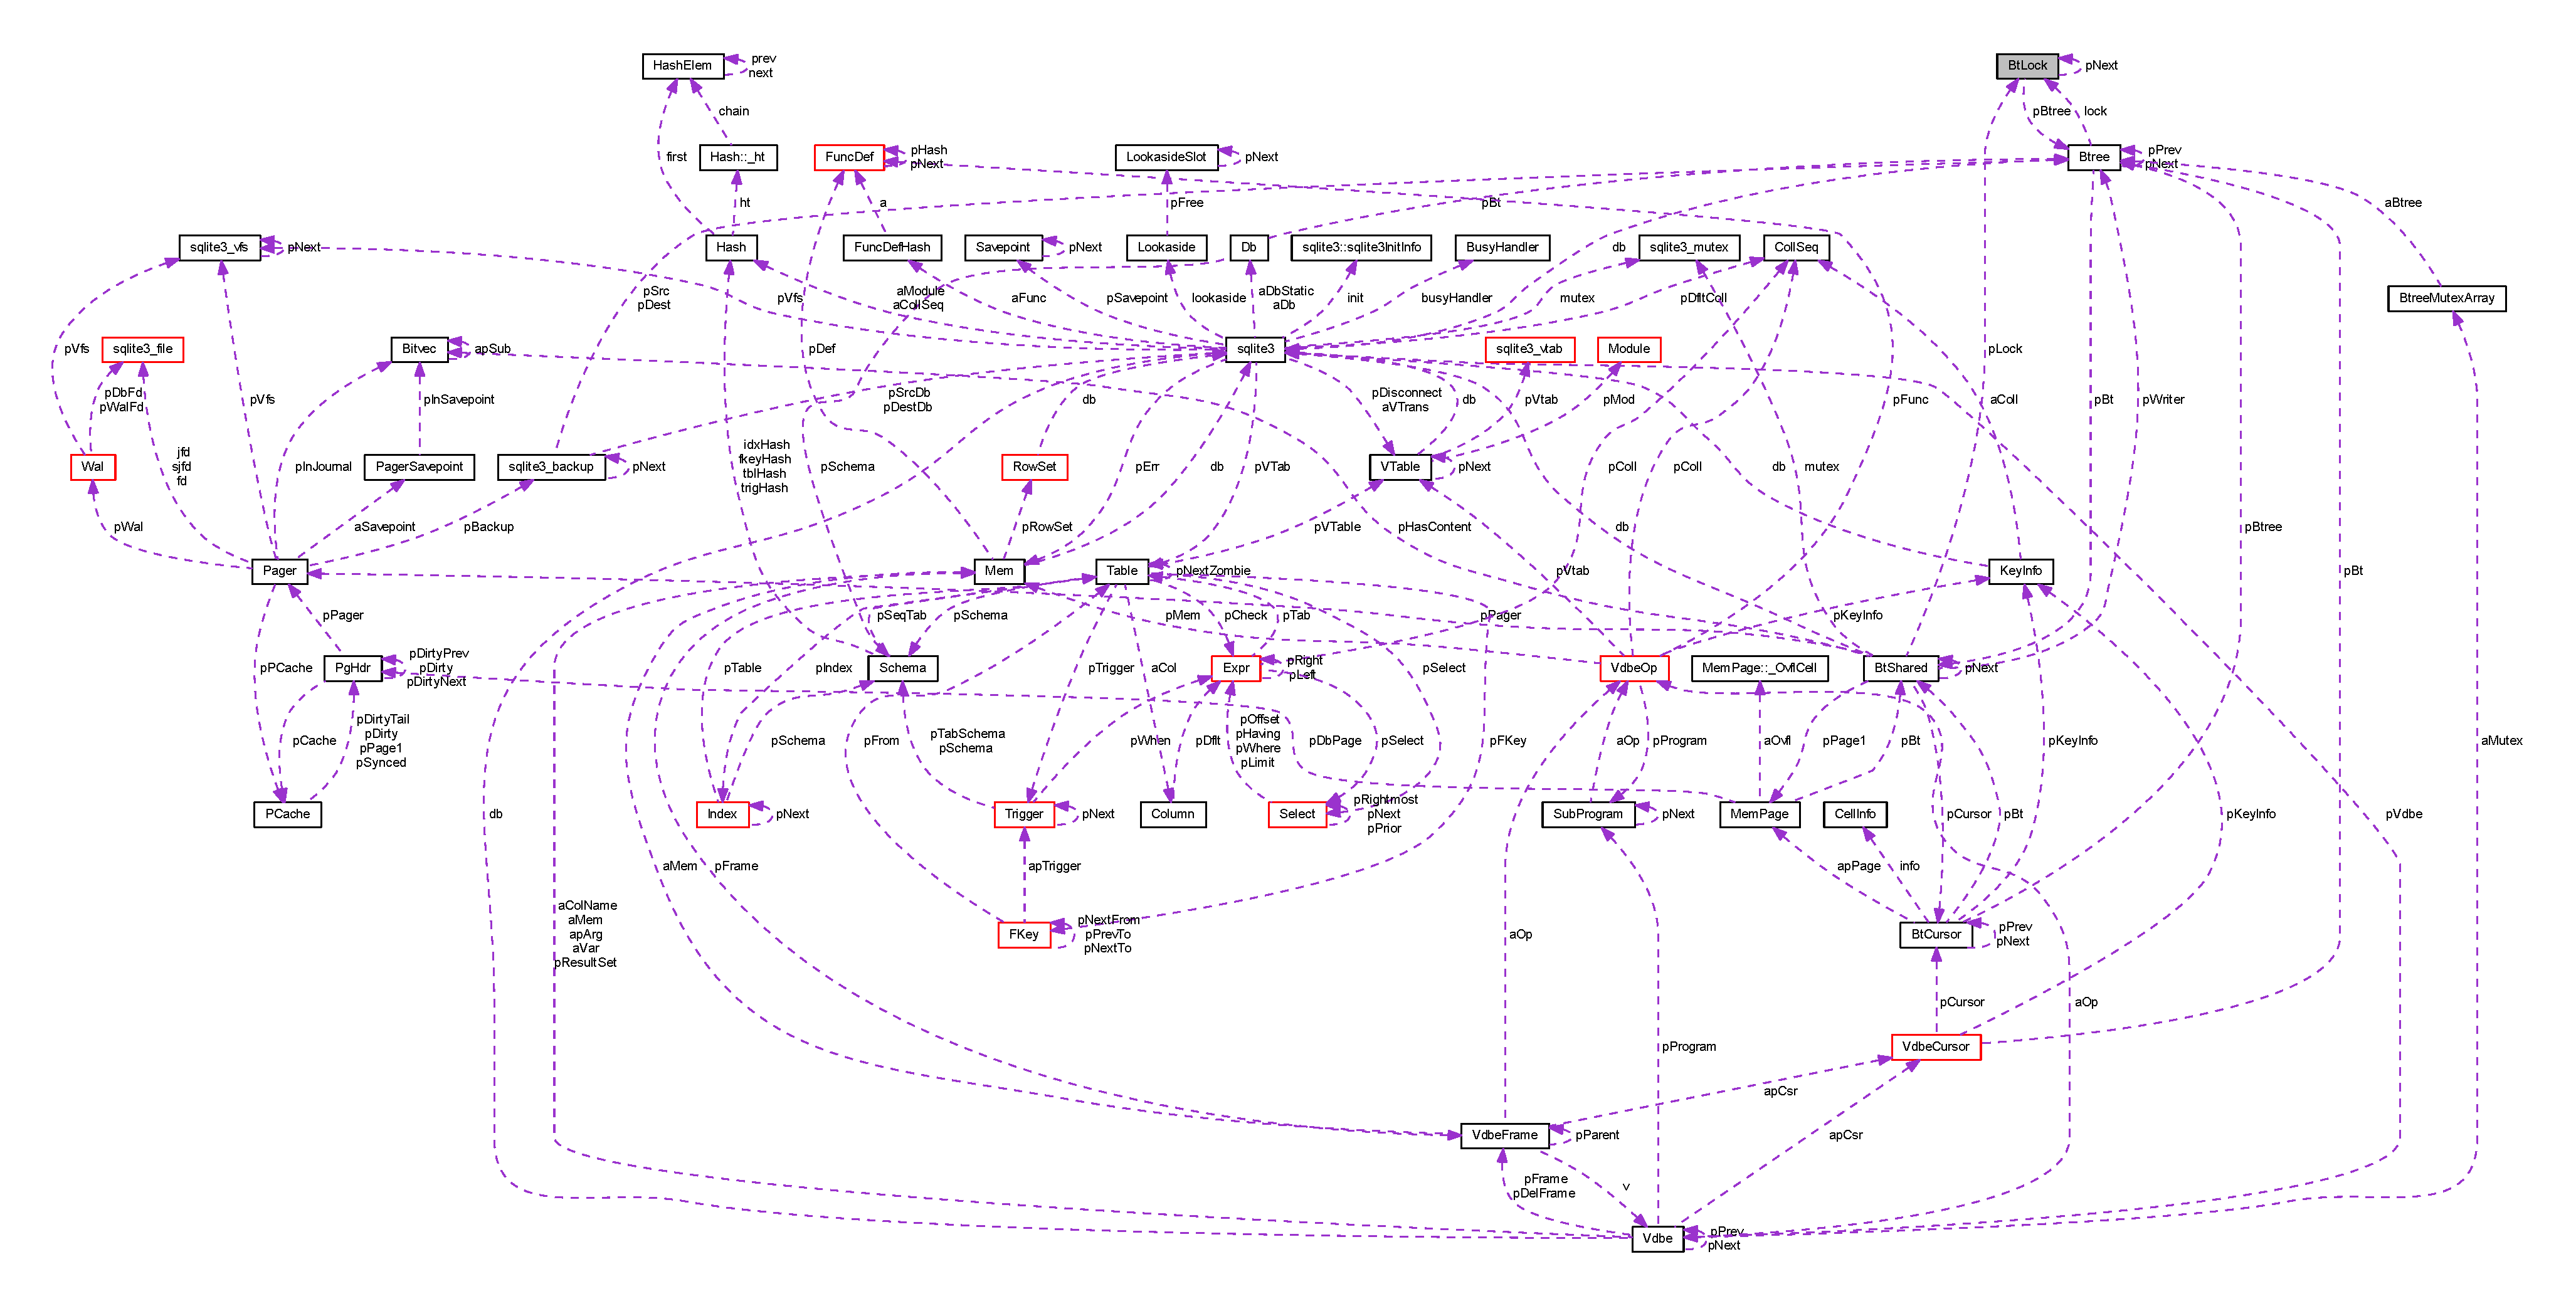
\includegraphics[width=350pt]{struct_bt_lock__coll__graph}
\end{center}
\end{figure}
\subsection*{Public Attributes}
\begin{DoxyCompactItemize}
\item 
\hypertarget{struct_bt_lock_ab9125b8e79d480b75f3af21cb2ab55c7}{\hyperlink{struct_btree}{Btree} $\ast$ {\bfseries p\-Btree}}\label{struct_bt_lock_ab9125b8e79d480b75f3af21cb2ab55c7}

\item 
\hypertarget{struct_bt_lock_a822efcf018d6c8eb343341cde5df980d}{Pgno {\bfseries i\-Table}}\label{struct_bt_lock_a822efcf018d6c8eb343341cde5df980d}

\item 
\hypertarget{struct_bt_lock_abe07b71018ee423e0d94b5cdba044b5c}{u8 {\bfseries e\-Lock}}\label{struct_bt_lock_abe07b71018ee423e0d94b5cdba044b5c}

\item 
\hypertarget{struct_bt_lock_ad42de86209c7aab43604c52a549b7bca}{\hyperlink{struct_bt_lock}{Bt\-Lock} $\ast$ {\bfseries p\-Next}}\label{struct_bt_lock_ad42de86209c7aab43604c52a549b7bca}

\end{DoxyCompactItemize}


The documentation for this struct was generated from the following file\-:\begin{DoxyCompactItemize}
\item 
C\-:/\-Users/\-Vitor/\-Desktop/\-Work\-Space/\-P\-R\-O\-J\-E\-T\-O\-\_\-\-F\-I\-N\-A\-L\-\_\-\-P\-O\-O/\-P\-R\-O\-J\-E\-T\-O\-\_\-\-D\-E\-V/\-P\-R\-O\-J\-E\-T\-O/\-Projeto\-\_\-codeblocks/sqlite3.\-c\end{DoxyCompactItemize}

\hypertarget{struct_btree}{\section{Btree Struct Reference}
\label{struct_btree}\index{Btree@{Btree}}
}


Collaboration diagram for Btree\-:\nopagebreak
\begin{figure}[H]
\begin{center}
\leavevmode
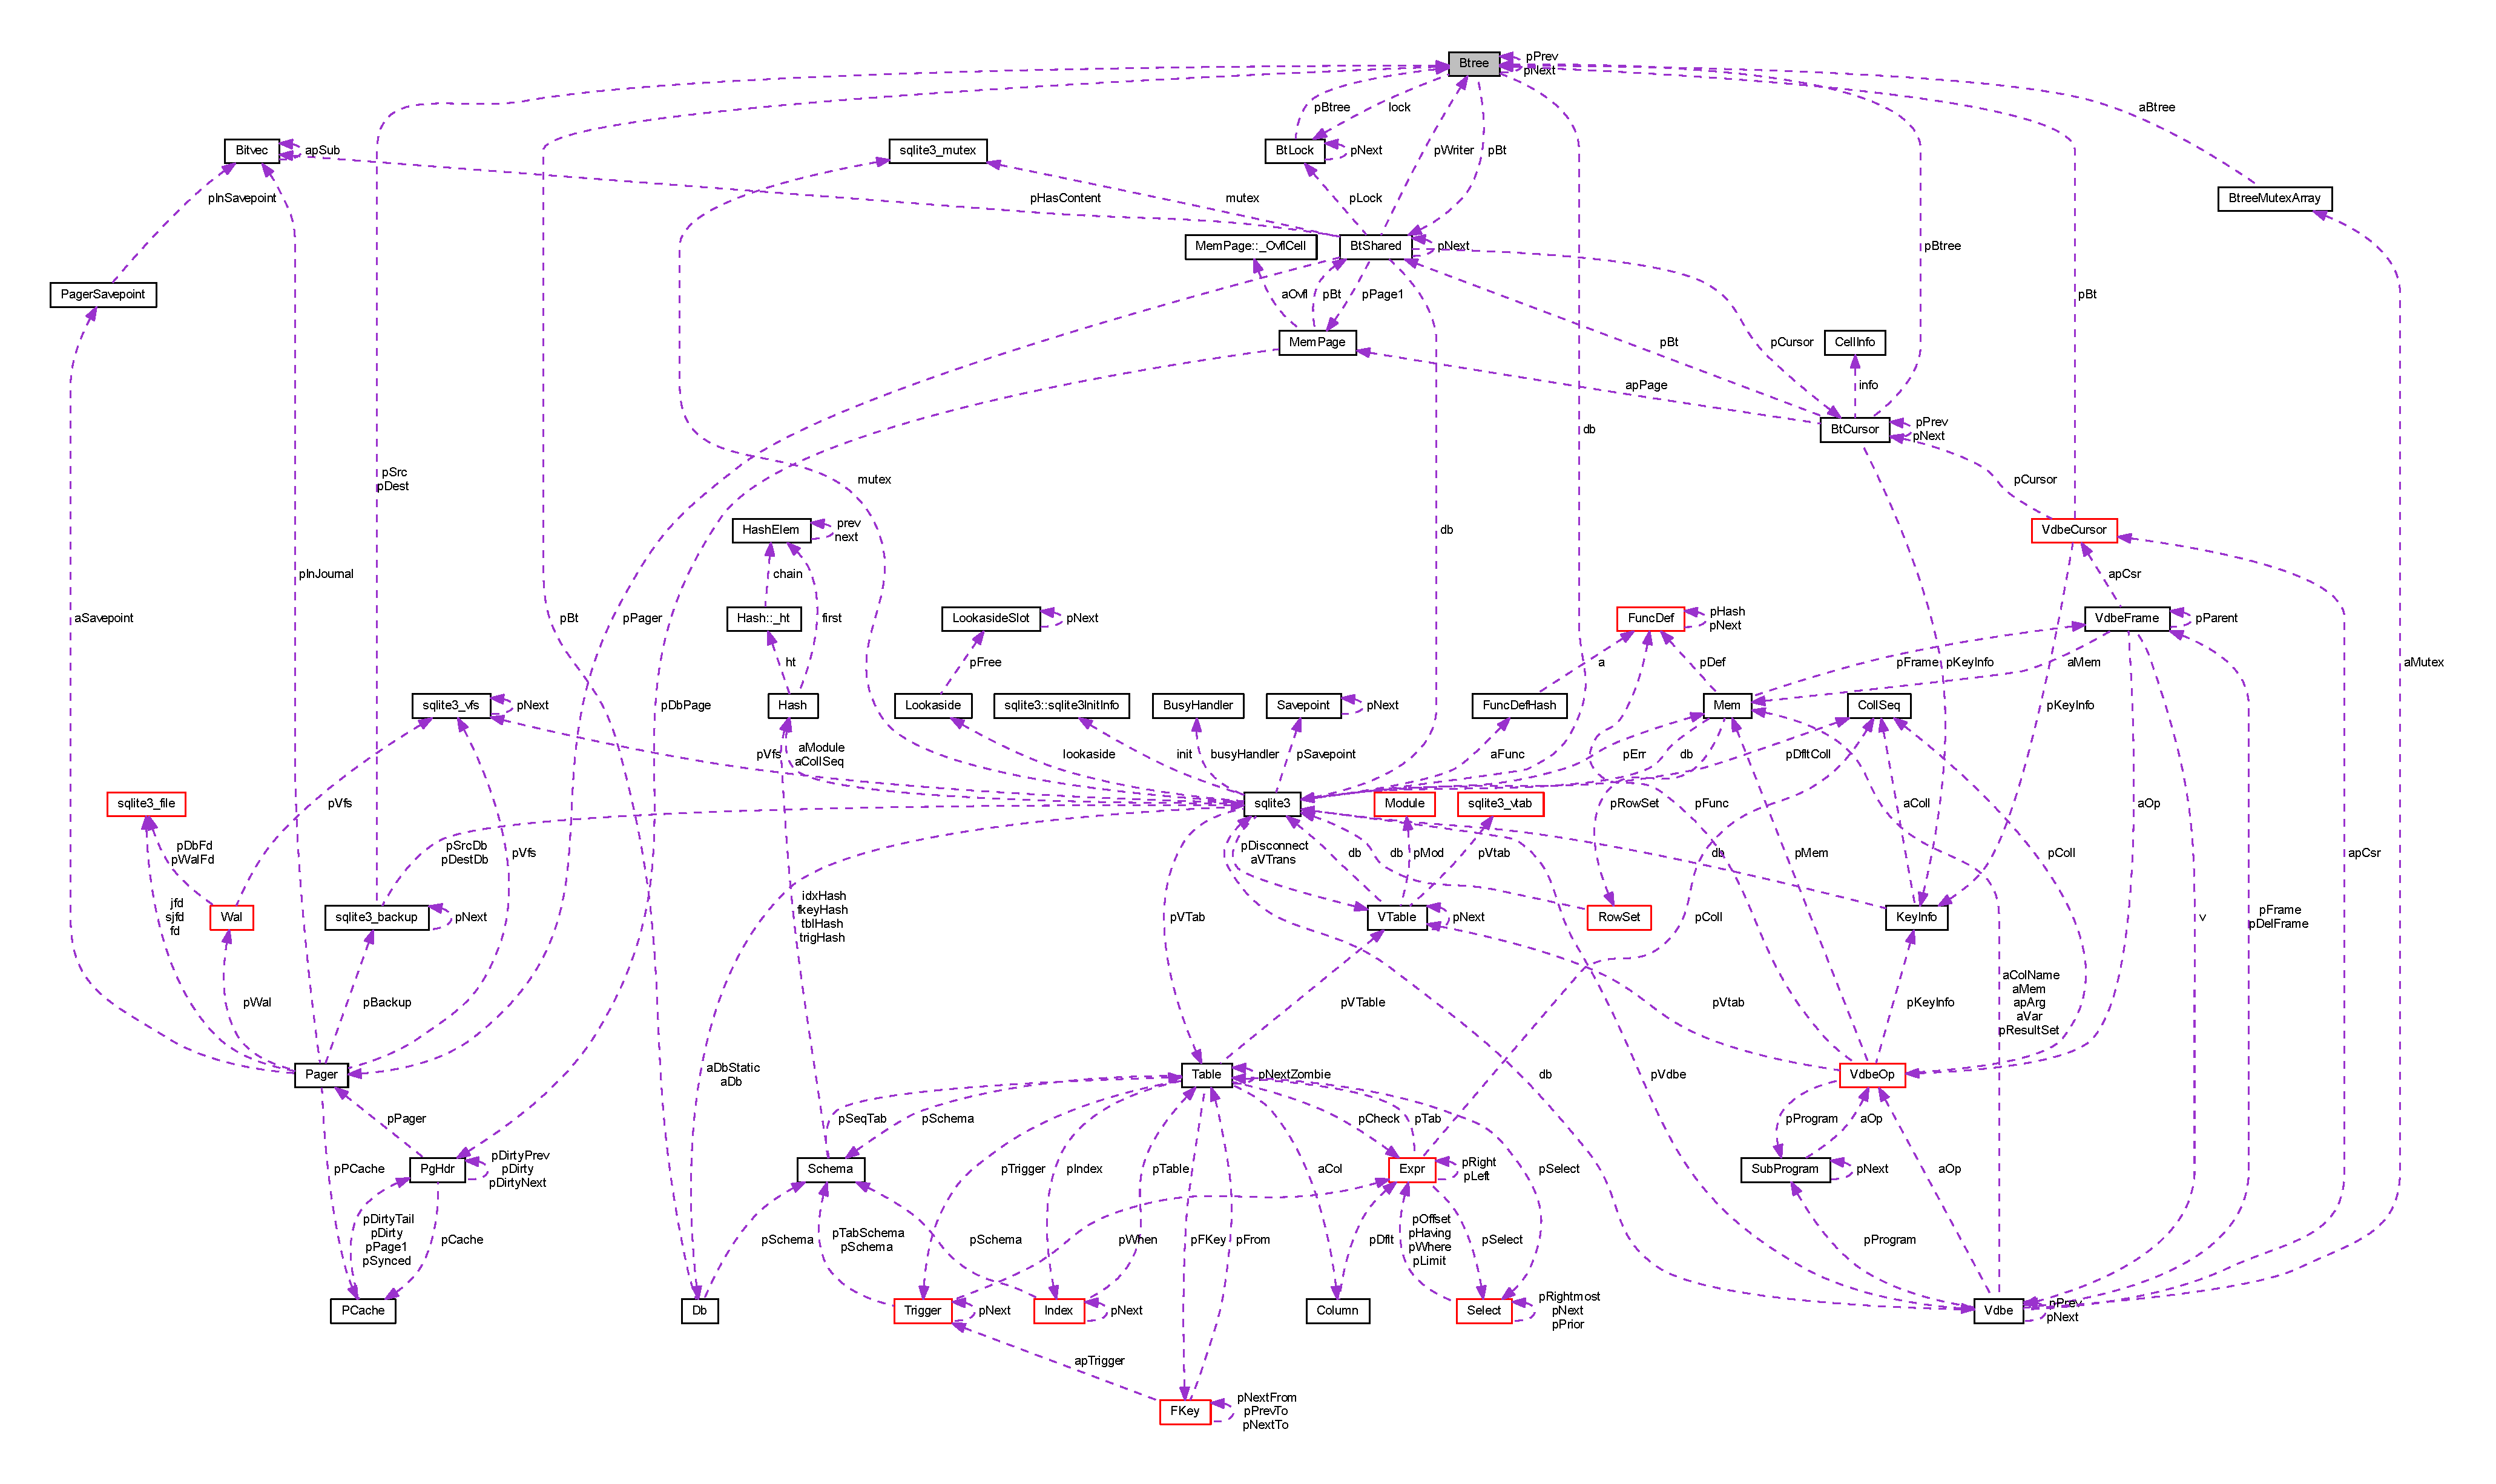
\includegraphics[width=350pt]{struct_btree__coll__graph}
\end{center}
\end{figure}
\subsection*{Public Attributes}
\begin{DoxyCompactItemize}
\item 
\hypertarget{struct_btree_a2b3cfec48b6e9fcfd641d433816ae5c3}{\hyperlink{structsqlite3}{sqlite3} $\ast$ {\bfseries db}}\label{struct_btree_a2b3cfec48b6e9fcfd641d433816ae5c3}

\item 
\hypertarget{struct_btree_a63bab5d744d48d14368af048dddf2f20}{\hyperlink{struct_bt_shared}{Bt\-Shared} $\ast$ {\bfseries p\-Bt}}\label{struct_btree_a63bab5d744d48d14368af048dddf2f20}

\item 
\hypertarget{struct_btree_a50007448960c05dfd1fdc7db3e277685}{u8 {\bfseries in\-Trans}}\label{struct_btree_a50007448960c05dfd1fdc7db3e277685}

\item 
\hypertarget{struct_btree_a114f157127c76a1fbad8292e4b39c4dd}{u8 {\bfseries sharable}}\label{struct_btree_a114f157127c76a1fbad8292e4b39c4dd}

\item 
\hypertarget{struct_btree_a16fc8292bae9a66cfec03f6cb82d06a8}{u8 {\bfseries locked}}\label{struct_btree_a16fc8292bae9a66cfec03f6cb82d06a8}

\item 
\hypertarget{struct_btree_a97368ea300f0b74b8e80ea07da0cea2a}{int {\bfseries want\-To\-Lock}}\label{struct_btree_a97368ea300f0b74b8e80ea07da0cea2a}

\item 
\hypertarget{struct_btree_a7a3e7cf38bc9c3021a9e270a54ecfb1e}{int {\bfseries n\-Backup}}\label{struct_btree_a7a3e7cf38bc9c3021a9e270a54ecfb1e}

\item 
\hypertarget{struct_btree_a9e6d2ca44c10ed8ef0be004225a74ef5}{\hyperlink{struct_btree}{Btree} $\ast$ {\bfseries p\-Next}}\label{struct_btree_a9e6d2ca44c10ed8ef0be004225a74ef5}

\item 
\hypertarget{struct_btree_a0423f1c55c1fe6812161a49bb2bf604f}{\hyperlink{struct_btree}{Btree} $\ast$ {\bfseries p\-Prev}}\label{struct_btree_a0423f1c55c1fe6812161a49bb2bf604f}

\item 
\hypertarget{struct_btree_a943ed8799c9943f753a88cf44f1632dc}{\hyperlink{struct_bt_lock}{Bt\-Lock} {\bfseries lock}}\label{struct_btree_a943ed8799c9943f753a88cf44f1632dc}

\end{DoxyCompactItemize}


The documentation for this struct was generated from the following file\-:\begin{DoxyCompactItemize}
\item 
sqlite3.\-c\end{DoxyCompactItemize}

\hypertarget{struct_btree_mutex_array}{\section{Btree\-Mutex\-Array Struct Reference}
\label{struct_btree_mutex_array}\index{Btree\-Mutex\-Array@{Btree\-Mutex\-Array}}
}


Collaboration diagram for Btree\-Mutex\-Array\-:\nopagebreak
\begin{figure}[H]
\begin{center}
\leavevmode
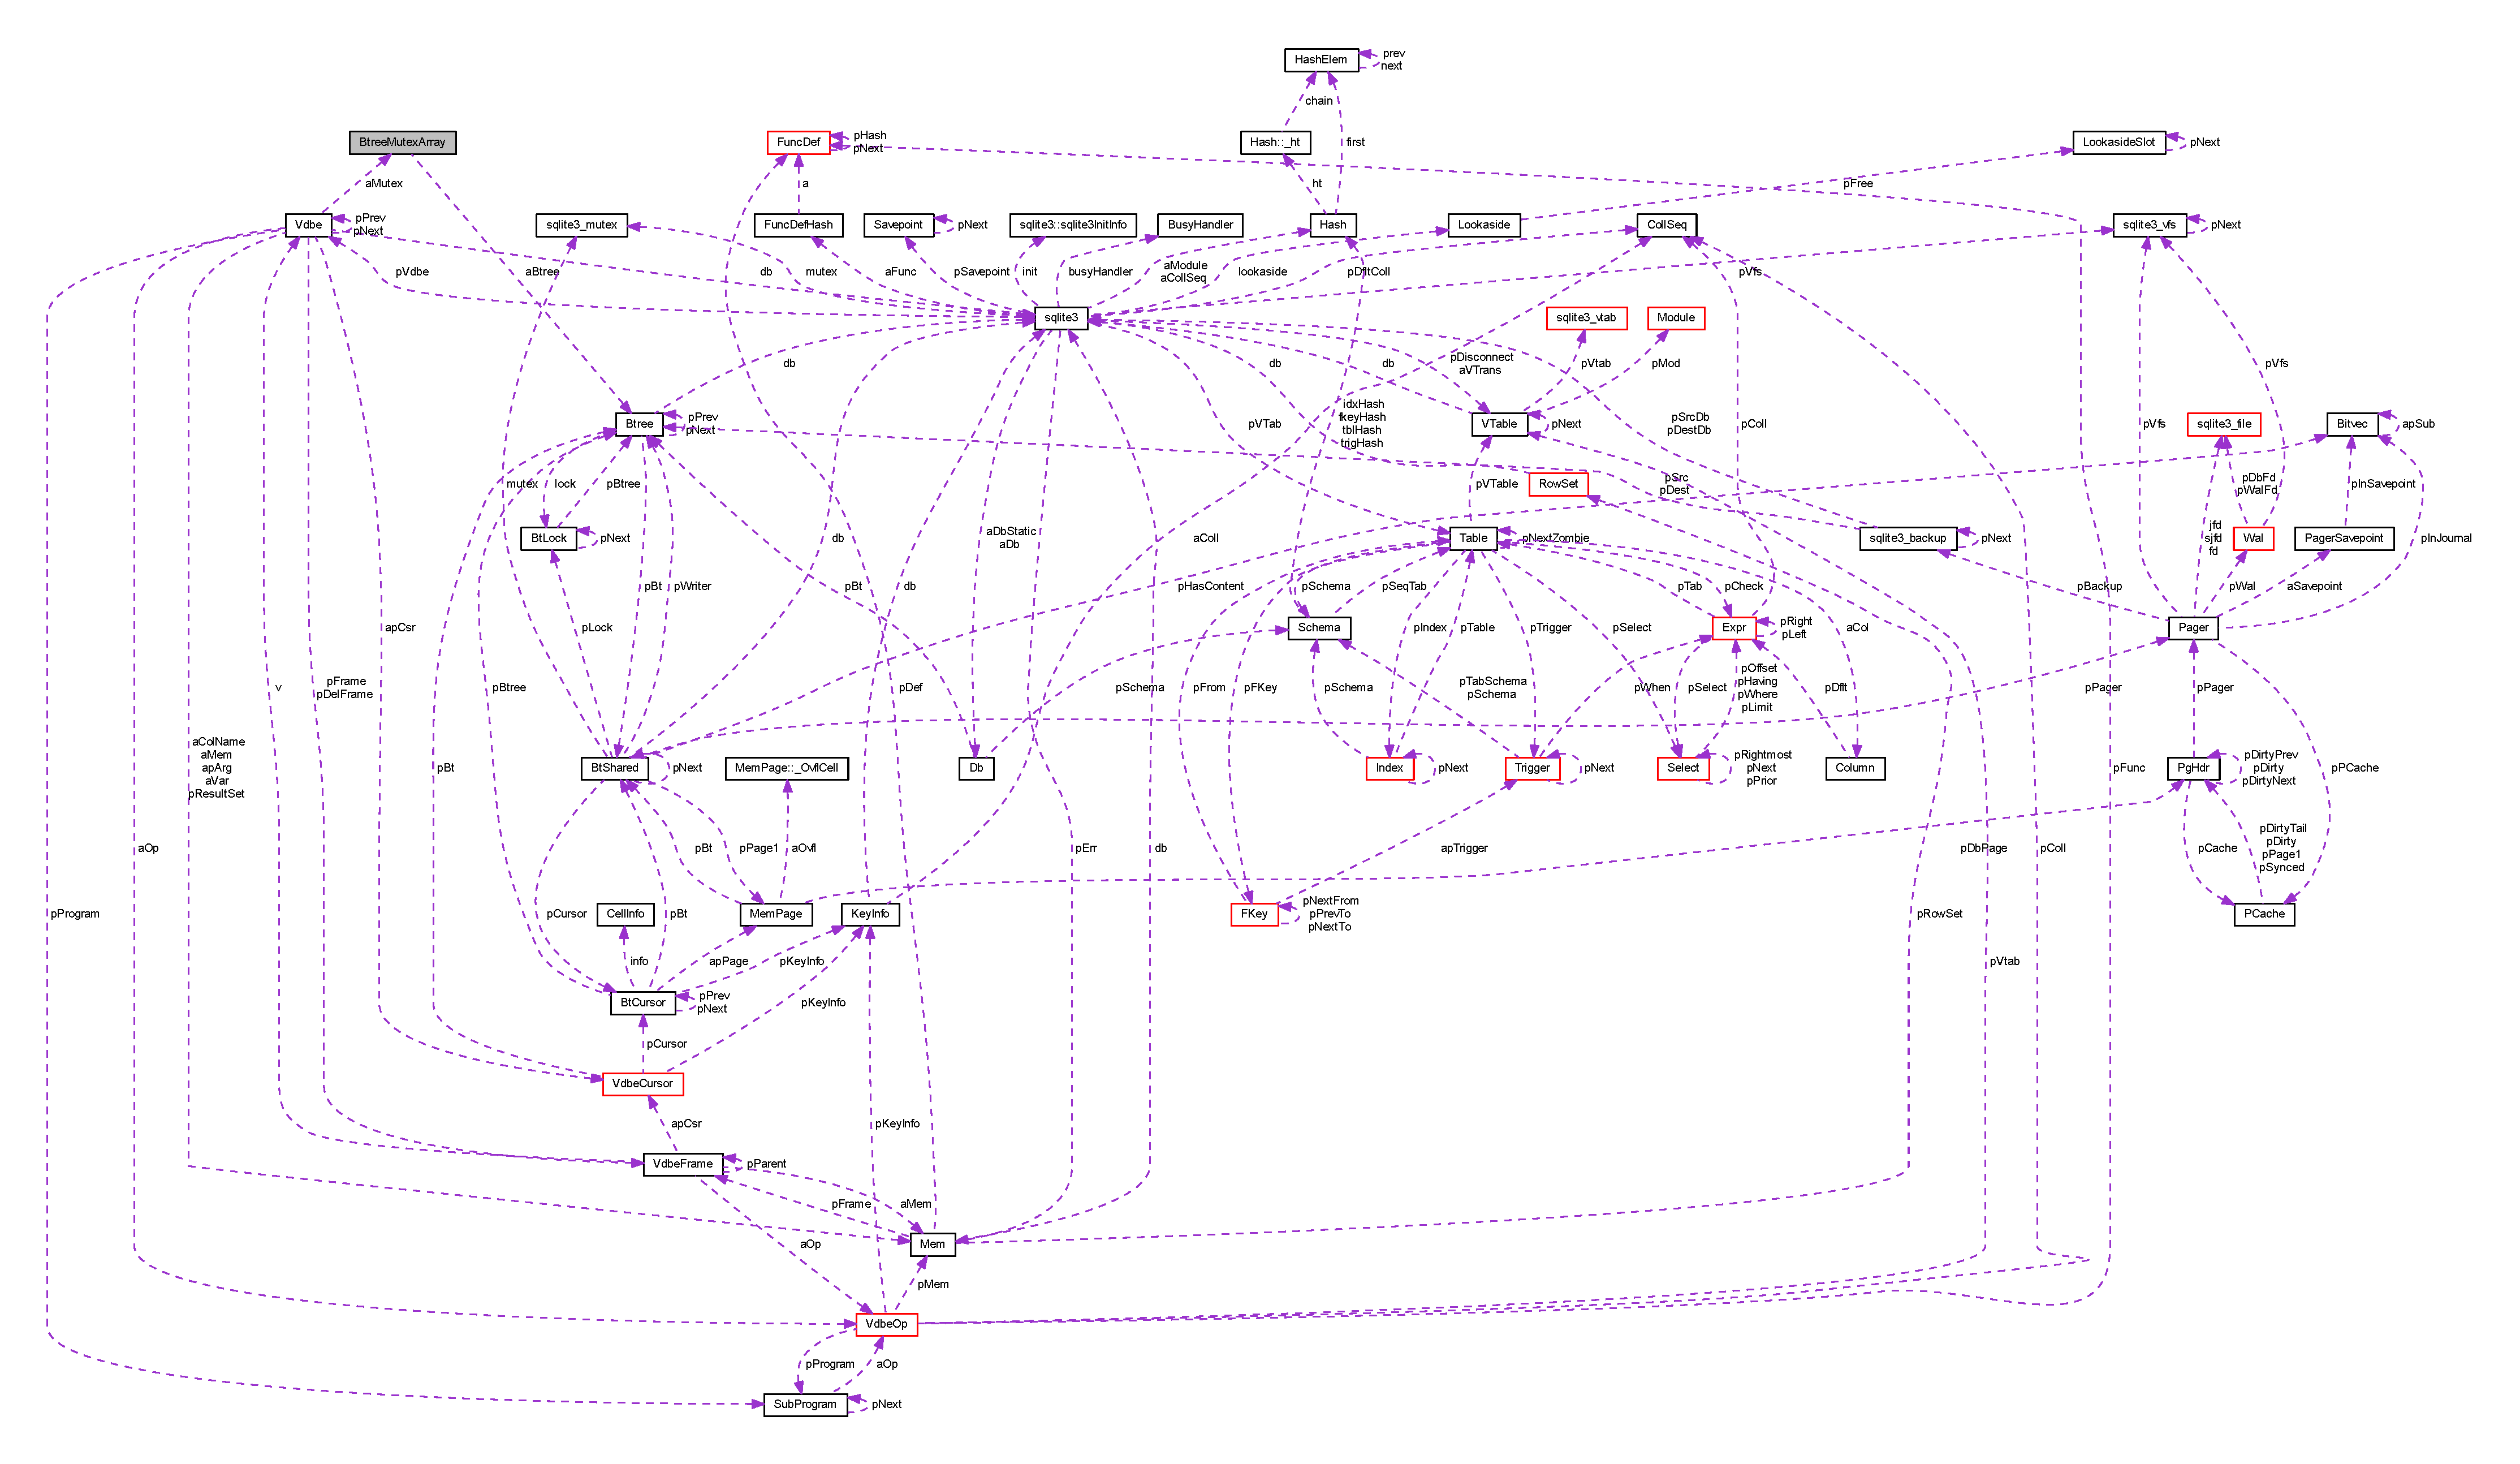
\includegraphics[width=350pt]{struct_btree_mutex_array__coll__graph}
\end{center}
\end{figure}
\subsection*{Public Attributes}
\begin{DoxyCompactItemize}
\item 
\hypertarget{struct_btree_mutex_array_a1c1e4c51a9ed52ea59152831bf7fc442}{int {\bfseries n\-Mutex}}\label{struct_btree_mutex_array_a1c1e4c51a9ed52ea59152831bf7fc442}

\item 
\hypertarget{struct_btree_mutex_array_ac5bbf3594cd584c88df9cb25731e26dc}{\hyperlink{struct_btree}{Btree} $\ast$ {\bfseries a\-Btree} \mbox{[}S\-Q\-L\-I\-T\-E\-\_\-\-M\-A\-X\-\_\-\-A\-T\-T\-A\-C\-H\-E\-D+1\mbox{]}}\label{struct_btree_mutex_array_ac5bbf3594cd584c88df9cb25731e26dc}

\end{DoxyCompactItemize}


The documentation for this struct was generated from the following file\-:\begin{DoxyCompactItemize}
\item 
sqlite3.\-c\end{DoxyCompactItemize}

\hypertarget{struct_bt_shared}{\section{Bt\-Shared Struct Reference}
\label{struct_bt_shared}\index{Bt\-Shared@{Bt\-Shared}}
}


Collaboration diagram for Bt\-Shared\-:\nopagebreak
\begin{figure}[H]
\begin{center}
\leavevmode
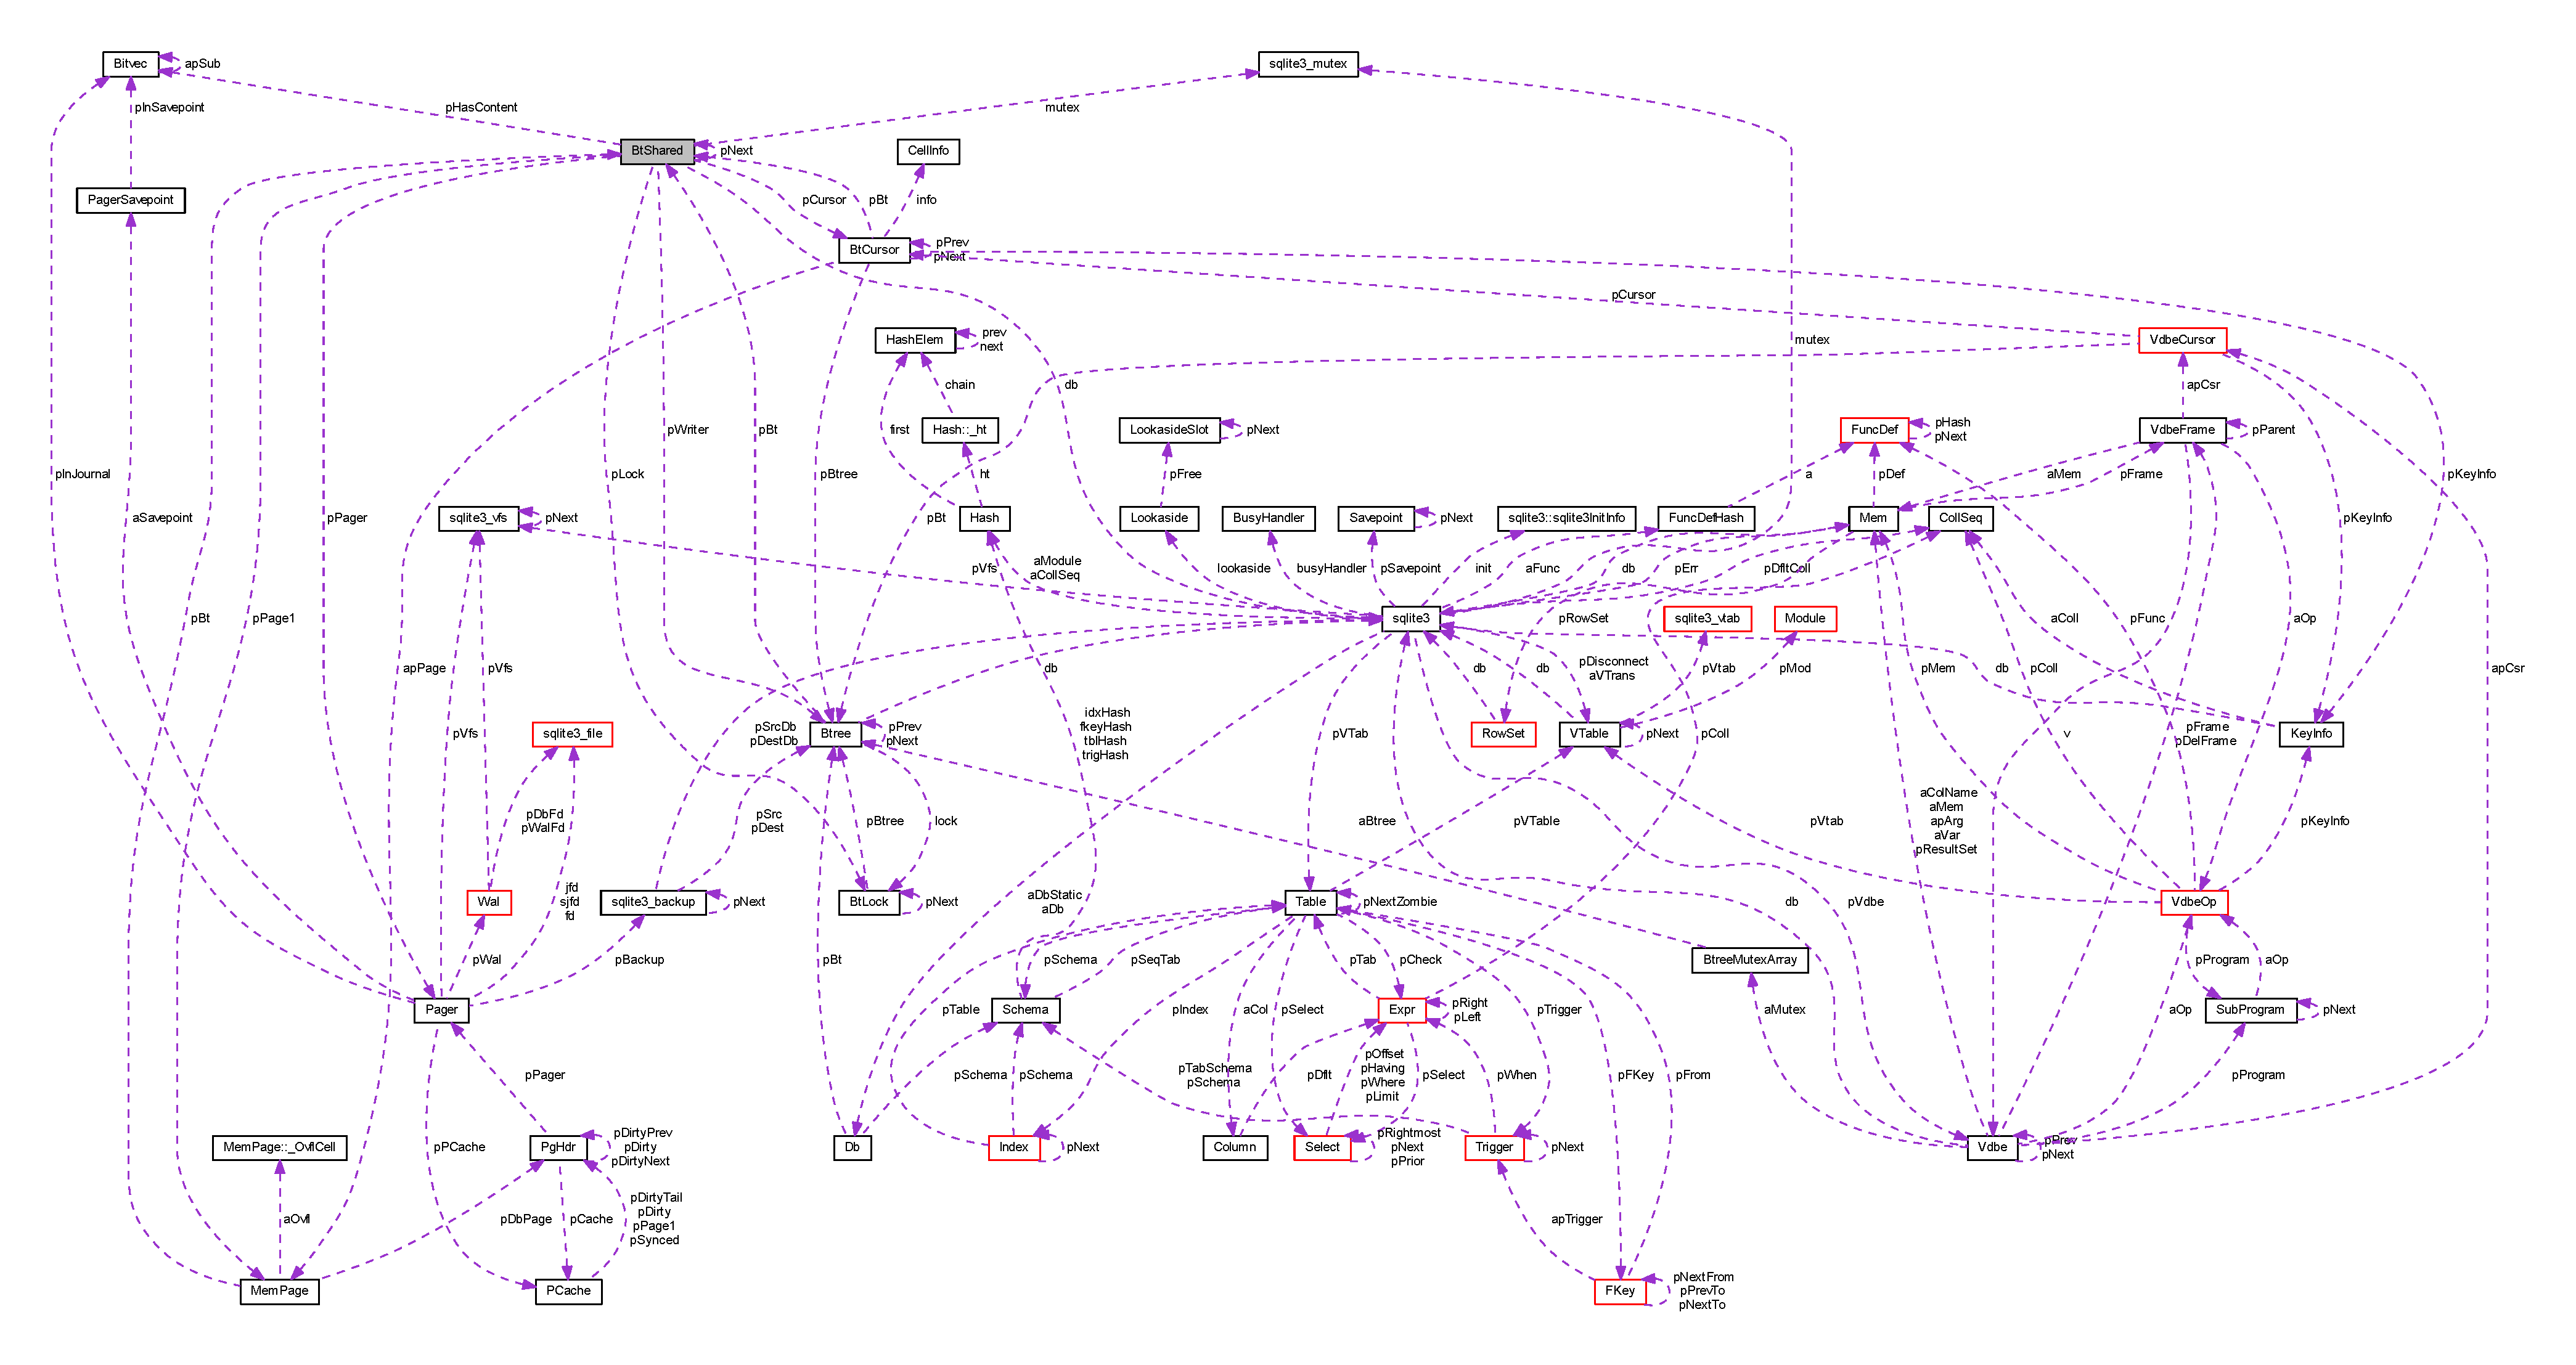
\includegraphics[width=350pt]{struct_bt_shared__coll__graph}
\end{center}
\end{figure}
\subsection*{Public Attributes}
\begin{DoxyCompactItemize}
\item 
\hypertarget{struct_bt_shared_ab79703fc47a16446274457588d7eb989}{\hyperlink{struct_pager}{Pager} $\ast$ {\bfseries p\-Pager}}\label{struct_bt_shared_ab79703fc47a16446274457588d7eb989}

\item 
\hypertarget{struct_bt_shared_a93dafa672793f6117a336d5987951c8e}{\hyperlink{structsqlite3}{sqlite3} $\ast$ {\bfseries db}}\label{struct_bt_shared_a93dafa672793f6117a336d5987951c8e}

\item 
\hypertarget{struct_bt_shared_a8f8b52dee390e5606e8e2a8511530de7}{\hyperlink{struct_bt_cursor}{Bt\-Cursor} $\ast$ {\bfseries p\-Cursor}}\label{struct_bt_shared_a8f8b52dee390e5606e8e2a8511530de7}

\item 
\hypertarget{struct_bt_shared_a296dffd1c698ec175fee109718f32d5d}{\hyperlink{struct_mem_page}{Mem\-Page} $\ast$ {\bfseries p\-Page1}}\label{struct_bt_shared_a296dffd1c698ec175fee109718f32d5d}

\item 
\hypertarget{struct_bt_shared_ac8e55afc249f7ffa3d0f5dd5637d3825}{u8 {\bfseries read\-Only}}\label{struct_bt_shared_ac8e55afc249f7ffa3d0f5dd5637d3825}

\item 
\hypertarget{struct_bt_shared_a0e728415ef91a26a8a1c6c9a6a9d8cd0}{u8 {\bfseries page\-Size\-Fixed}}\label{struct_bt_shared_a0e728415ef91a26a8a1c6c9a6a9d8cd0}

\item 
\hypertarget{struct_bt_shared_af8fe491f61d5c4be043dc19aa0bda0c4}{u8 {\bfseries secure\-Delete}}\label{struct_bt_shared_af8fe491f61d5c4be043dc19aa0bda0c4}

\item 
\hypertarget{struct_bt_shared_a48779c116d7bad3616fe36bd81bb01c2}{u8 {\bfseries initially\-Empty}}\label{struct_bt_shared_a48779c116d7bad3616fe36bd81bb01c2}

\item 
\hypertarget{struct_bt_shared_a8fbc250e23d7c417ccfec8cceb08329d}{u8 {\bfseries open\-Flags}}\label{struct_bt_shared_a8fbc250e23d7c417ccfec8cceb08329d}

\item 
\hypertarget{struct_bt_shared_a770c4f6244d4350f27029cb909902a61}{u8 {\bfseries auto\-Vacuum}}\label{struct_bt_shared_a770c4f6244d4350f27029cb909902a61}

\item 
\hypertarget{struct_bt_shared_a8d8ba06335a63d8a36294a0f1ae8377a}{u8 {\bfseries incr\-Vacuum}}\label{struct_bt_shared_a8d8ba06335a63d8a36294a0f1ae8377a}

\item 
\hypertarget{struct_bt_shared_a2937d14071841fe0ecae3ce1eb1da96c}{u16 {\bfseries max\-Local}}\label{struct_bt_shared_a2937d14071841fe0ecae3ce1eb1da96c}

\item 
\hypertarget{struct_bt_shared_affb40500b5c63601ef3ca3600983b12c}{u16 {\bfseries min\-Local}}\label{struct_bt_shared_affb40500b5c63601ef3ca3600983b12c}

\item 
\hypertarget{struct_bt_shared_a474248f018d24457ec306a7b570d24ce}{u16 {\bfseries max\-Leaf}}\label{struct_bt_shared_a474248f018d24457ec306a7b570d24ce}

\item 
\hypertarget{struct_bt_shared_ad57c14f1681d0e86f1c9a9488013eba0}{u16 {\bfseries min\-Leaf}}\label{struct_bt_shared_ad57c14f1681d0e86f1c9a9488013eba0}

\item 
\hypertarget{struct_bt_shared_aeaa6c0f33b83434ecee4bd8c4c8df48e}{u8 {\bfseries in\-Transaction}}\label{struct_bt_shared_aeaa6c0f33b83434ecee4bd8c4c8df48e}

\item 
\hypertarget{struct_bt_shared_a50bdaa76c7f59233533ca9d39567f7ce}{u8 {\bfseries do\-Not\-Use\-W\-A\-L}}\label{struct_bt_shared_a50bdaa76c7f59233533ca9d39567f7ce}

\item 
\hypertarget{struct_bt_shared_a9e42a71e5e3f98ec1e5b30998b27aae0}{u32 {\bfseries page\-Size}}\label{struct_bt_shared_a9e42a71e5e3f98ec1e5b30998b27aae0}

\item 
\hypertarget{struct_bt_shared_a3209efe543084a7e60f22913a794f5cb}{u32 {\bfseries usable\-Size}}\label{struct_bt_shared_a3209efe543084a7e60f22913a794f5cb}

\item 
\hypertarget{struct_bt_shared_a6101a0e79a95e884ac4dc9c70a947715}{int {\bfseries n\-Transaction}}\label{struct_bt_shared_a6101a0e79a95e884ac4dc9c70a947715}

\item 
\hypertarget{struct_bt_shared_a8679241243f9043ede97b5c57d20c3ea}{u32 {\bfseries n\-Page}}\label{struct_bt_shared_a8679241243f9043ede97b5c57d20c3ea}

\item 
\hypertarget{struct_bt_shared_aea3ccb6775c768fbd4f3e29df8cb925d}{void $\ast$ {\bfseries p\-Schema}}\label{struct_bt_shared_aea3ccb6775c768fbd4f3e29df8cb925d}

\item 
\hypertarget{struct_bt_shared_a7c4816c63acea30ed44ffc58b468463e}{void($\ast$ {\bfseries x\-Free\-Schema} )(void $\ast$)}\label{struct_bt_shared_a7c4816c63acea30ed44ffc58b468463e}

\item 
\hypertarget{struct_bt_shared_a454c31d726220bbed43c165e370460c8}{\hyperlink{structsqlite3__mutex}{sqlite3\-\_\-mutex} $\ast$ {\bfseries mutex}}\label{struct_bt_shared_a454c31d726220bbed43c165e370460c8}

\item 
\hypertarget{struct_bt_shared_ace6191dc3f48f9575d7946ab8cf5b919}{\hyperlink{struct_bitvec}{Bitvec} $\ast$ {\bfseries p\-Has\-Content}}\label{struct_bt_shared_ace6191dc3f48f9575d7946ab8cf5b919}

\item 
\hypertarget{struct_bt_shared_a43d0226fa08d7fae5f992f3a2d72cc08}{int {\bfseries n\-Ref}}\label{struct_bt_shared_a43d0226fa08d7fae5f992f3a2d72cc08}

\item 
\hypertarget{struct_bt_shared_aaa9dd5c5d4ec2bb79ebe4b37ee926ae3}{\hyperlink{struct_bt_shared}{Bt\-Shared} $\ast$ {\bfseries p\-Next}}\label{struct_bt_shared_aaa9dd5c5d4ec2bb79ebe4b37ee926ae3}

\item 
\hypertarget{struct_bt_shared_af58c79eec88f99ed5a07d8cabf8a1d1a}{\hyperlink{struct_bt_lock}{Bt\-Lock} $\ast$ {\bfseries p\-Lock}}\label{struct_bt_shared_af58c79eec88f99ed5a07d8cabf8a1d1a}

\item 
\hypertarget{struct_bt_shared_ad8b2679e54027d58a3be3afcca4df1d6}{\hyperlink{struct_btree}{Btree} $\ast$ {\bfseries p\-Writer}}\label{struct_bt_shared_ad8b2679e54027d58a3be3afcca4df1d6}

\item 
\hypertarget{struct_bt_shared_a416a0c0b3e26ed2ffff7e5e0cad53dc2}{u8 {\bfseries is\-Exclusive}}\label{struct_bt_shared_a416a0c0b3e26ed2ffff7e5e0cad53dc2}

\item 
\hypertarget{struct_bt_shared_accae7a07dc99dc2de544d437ab265191}{u8 {\bfseries is\-Pending}}\label{struct_bt_shared_accae7a07dc99dc2de544d437ab265191}

\item 
\hypertarget{struct_bt_shared_a89102c20327da8a304f7e95af557bdf4}{u8 $\ast$ {\bfseries p\-Tmp\-Space}}\label{struct_bt_shared_a89102c20327da8a304f7e95af557bdf4}

\end{DoxyCompactItemize}


The documentation for this struct was generated from the following file\-:\begin{DoxyCompactItemize}
\item 
sqlite3.\-c\end{DoxyCompactItemize}

\hypertarget{class_builder}{\section{Builder Class Reference}
\label{class_builder}\index{Builder@{Builder}}
}


Essa e a classe responsavel por ser linkar as classes do programa.  




{\ttfamily \#include $<$Builder.\-h$>$}



\subsection{Detailed Description}
Essa e a classe responsavel por ser linkar as classes do programa. 

The documentation for this class was generated from the following files\-:\begin{DoxyCompactItemize}
\item 
C\-:/\-Users/\-Vitor/\-Desktop/\-Work\-Space/\-P\-R\-O\-J\-E\-T\-O\-\_\-\-F\-I\-N\-A\-L\-\_\-\-P\-O\-O/\-P\-R\-O\-J\-E\-T\-O\-\_\-\-D\-E\-V/\-P\-R\-O\-J\-E\-T\-O/\-Projeto\-\_\-codeblocks/\hyperlink{_builder_8h}{Builder.\-h}\item 
C\-:/\-Users/\-Vitor/\-Desktop/\-Work\-Space/\-P\-R\-O\-J\-E\-T\-O\-\_\-\-F\-I\-N\-A\-L\-\_\-\-P\-O\-O/\-P\-R\-O\-J\-E\-T\-O\-\_\-\-D\-E\-V/\-P\-R\-O\-J\-E\-T\-O/\-Projeto\-\_\-codeblocks/Builder.\-cpp\end{DoxyCompactItemize}

\hypertarget{struct_busy_handler}{\section{Busy\-Handler Struct Reference}
\label{struct_busy_handler}\index{Busy\-Handler@{Busy\-Handler}}
}
\subsection*{Public Attributes}
\begin{DoxyCompactItemize}
\item 
\hypertarget{struct_busy_handler_aafc84c4e4934de2d5bdf02f268e9340f}{int($\ast$ {\bfseries x\-Func} )(void $\ast$, int)}\label{struct_busy_handler_aafc84c4e4934de2d5bdf02f268e9340f}

\item 
\hypertarget{struct_busy_handler_a1c793d2b815e79cf3684de46847551bd}{void $\ast$ {\bfseries p\-Arg}}\label{struct_busy_handler_a1c793d2b815e79cf3684de46847551bd}

\item 
\hypertarget{struct_busy_handler_aac4531c677ed5ae9e4757ca1b02c568b}{int {\bfseries n\-Busy}}\label{struct_busy_handler_aac4531c677ed5ae9e4757ca1b02c568b}

\end{DoxyCompactItemize}


The documentation for this struct was generated from the following file\-:\begin{DoxyCompactItemize}
\item 
C\-:/\-Users/\-Vitor/\-Desktop/\-Work\-Space/\-P\-R\-O\-J\-E\-T\-O\-\_\-\-F\-I\-N\-A\-L\-\_\-\-P\-O\-O/\-P\-R\-O\-J\-E\-T\-O\-\_\-\-D\-E\-V/\-P\-R\-O\-J\-E\-T\-O/\-Projeto\-\_\-codeblocks/sqlite3.\-c\end{DoxyCompactItemize}

\hypertarget{struct_cell_info}{\section{Cell\-Info Struct Reference}
\label{struct_cell_info}\index{Cell\-Info@{Cell\-Info}}
}
\subsection*{Public Attributes}
\begin{DoxyCompactItemize}
\item 
\hypertarget{struct_cell_info_a595ed7eeb60ea274d868f24347b7238e}{u8 $\ast$ {\bfseries p\-Cell}}\label{struct_cell_info_a595ed7eeb60ea274d868f24347b7238e}

\item 
\hypertarget{struct_cell_info_a542b041b9a54a13f7c6f2fe63e7542c0}{i64 {\bfseries n\-Key}}\label{struct_cell_info_a542b041b9a54a13f7c6f2fe63e7542c0}

\item 
\hypertarget{struct_cell_info_af2301ed16c35633ec6b5d7792734a4bf}{u32 {\bfseries n\-Data}}\label{struct_cell_info_af2301ed16c35633ec6b5d7792734a4bf}

\item 
\hypertarget{struct_cell_info_ac1e3c1b4216a8e778bbac82907bb1485}{u32 {\bfseries n\-Payload}}\label{struct_cell_info_ac1e3c1b4216a8e778bbac82907bb1485}

\item 
\hypertarget{struct_cell_info_a99bb1f87208f793359cf63e3d164025b}{u16 {\bfseries n\-Header}}\label{struct_cell_info_a99bb1f87208f793359cf63e3d164025b}

\item 
\hypertarget{struct_cell_info_a8cedbcc2c94916fe5798b502c614bb08}{u16 {\bfseries n\-Local}}\label{struct_cell_info_a8cedbcc2c94916fe5798b502c614bb08}

\item 
\hypertarget{struct_cell_info_af7be0161f1c67600aeba783a68972f70}{u16 {\bfseries i\-Overflow}}\label{struct_cell_info_af7be0161f1c67600aeba783a68972f70}

\item 
\hypertarget{struct_cell_info_ace78ab5eb5337b686e31b895feeb0562}{u16 {\bfseries n\-Size}}\label{struct_cell_info_ace78ab5eb5337b686e31b895feeb0562}

\end{DoxyCompactItemize}


The documentation for this struct was generated from the following file\-:\begin{DoxyCompactItemize}
\item 
C\-:/\-Users/\-Vitor/\-Desktop/\-Work\-Space/\-P\-R\-O\-J\-E\-T\-O\-\_\-\-F\-I\-N\-A\-L\-\_\-\-P\-O\-O/\-P\-R\-O\-J\-E\-T\-O\-\_\-\-D\-E\-V/\-P\-R\-O\-J\-E\-T\-O/\-Projeto\-\_\-codeblocks/sqlite3.\-c\end{DoxyCompactItemize}

\hypertarget{struct_coll_seq}{\section{Coll\-Seq Struct Reference}
\label{struct_coll_seq}\index{Coll\-Seq@{Coll\-Seq}}
}
\subsection*{Public Attributes}
\begin{DoxyCompactItemize}
\item 
\hypertarget{struct_coll_seq_a48d6d5f71d4f8a3ab122903464e8b4a1}{char $\ast$ {\bfseries z\-Name}}\label{struct_coll_seq_a48d6d5f71d4f8a3ab122903464e8b4a1}

\item 
\hypertarget{struct_coll_seq_add27da1a70ed6f538447e9183eeb4838}{u8 {\bfseries enc}}\label{struct_coll_seq_add27da1a70ed6f538447e9183eeb4838}

\item 
\hypertarget{struct_coll_seq_ae8e3e561c3ff15d81758530573ceb5f9}{u8 {\bfseries type}}\label{struct_coll_seq_ae8e3e561c3ff15d81758530573ceb5f9}

\item 
\hypertarget{struct_coll_seq_a3cee924d41e730ccec7f686eb5b6f041}{void $\ast$ {\bfseries p\-User}}\label{struct_coll_seq_a3cee924d41e730ccec7f686eb5b6f041}

\item 
\hypertarget{struct_coll_seq_a47fc6d3a01eee354332ca515a8b493ce}{int($\ast$ {\bfseries x\-Cmp} )(void $\ast$, int, const void $\ast$, int, const void $\ast$)}\label{struct_coll_seq_a47fc6d3a01eee354332ca515a8b493ce}

\item 
\hypertarget{struct_coll_seq_a1c0dd3ad98c7bb2ef517f9170134a125}{void($\ast$ {\bfseries x\-Del} )(void $\ast$)}\label{struct_coll_seq_a1c0dd3ad98c7bb2ef517f9170134a125}

\end{DoxyCompactItemize}


The documentation for this struct was generated from the following file\-:\begin{DoxyCompactItemize}
\item 
C\-:/\-Users/\-Vitor/\-Desktop/\-Work\-Space/\-P\-R\-O\-J\-E\-T\-O\-\_\-\-F\-I\-N\-A\-L\-\_\-\-P\-O\-O/\-P\-R\-O\-J\-E\-T\-O\-\_\-\-D\-E\-V/\-P\-R\-O\-J\-E\-T\-O/\-Projeto\-\_\-codeblocks/sqlite3.\-c\end{DoxyCompactItemize}

\hypertarget{struct_column}{\section{Column Struct Reference}
\label{struct_column}\index{Column@{Column}}
}


Collaboration diagram for Column\-:\nopagebreak
\begin{figure}[H]
\begin{center}
\leavevmode
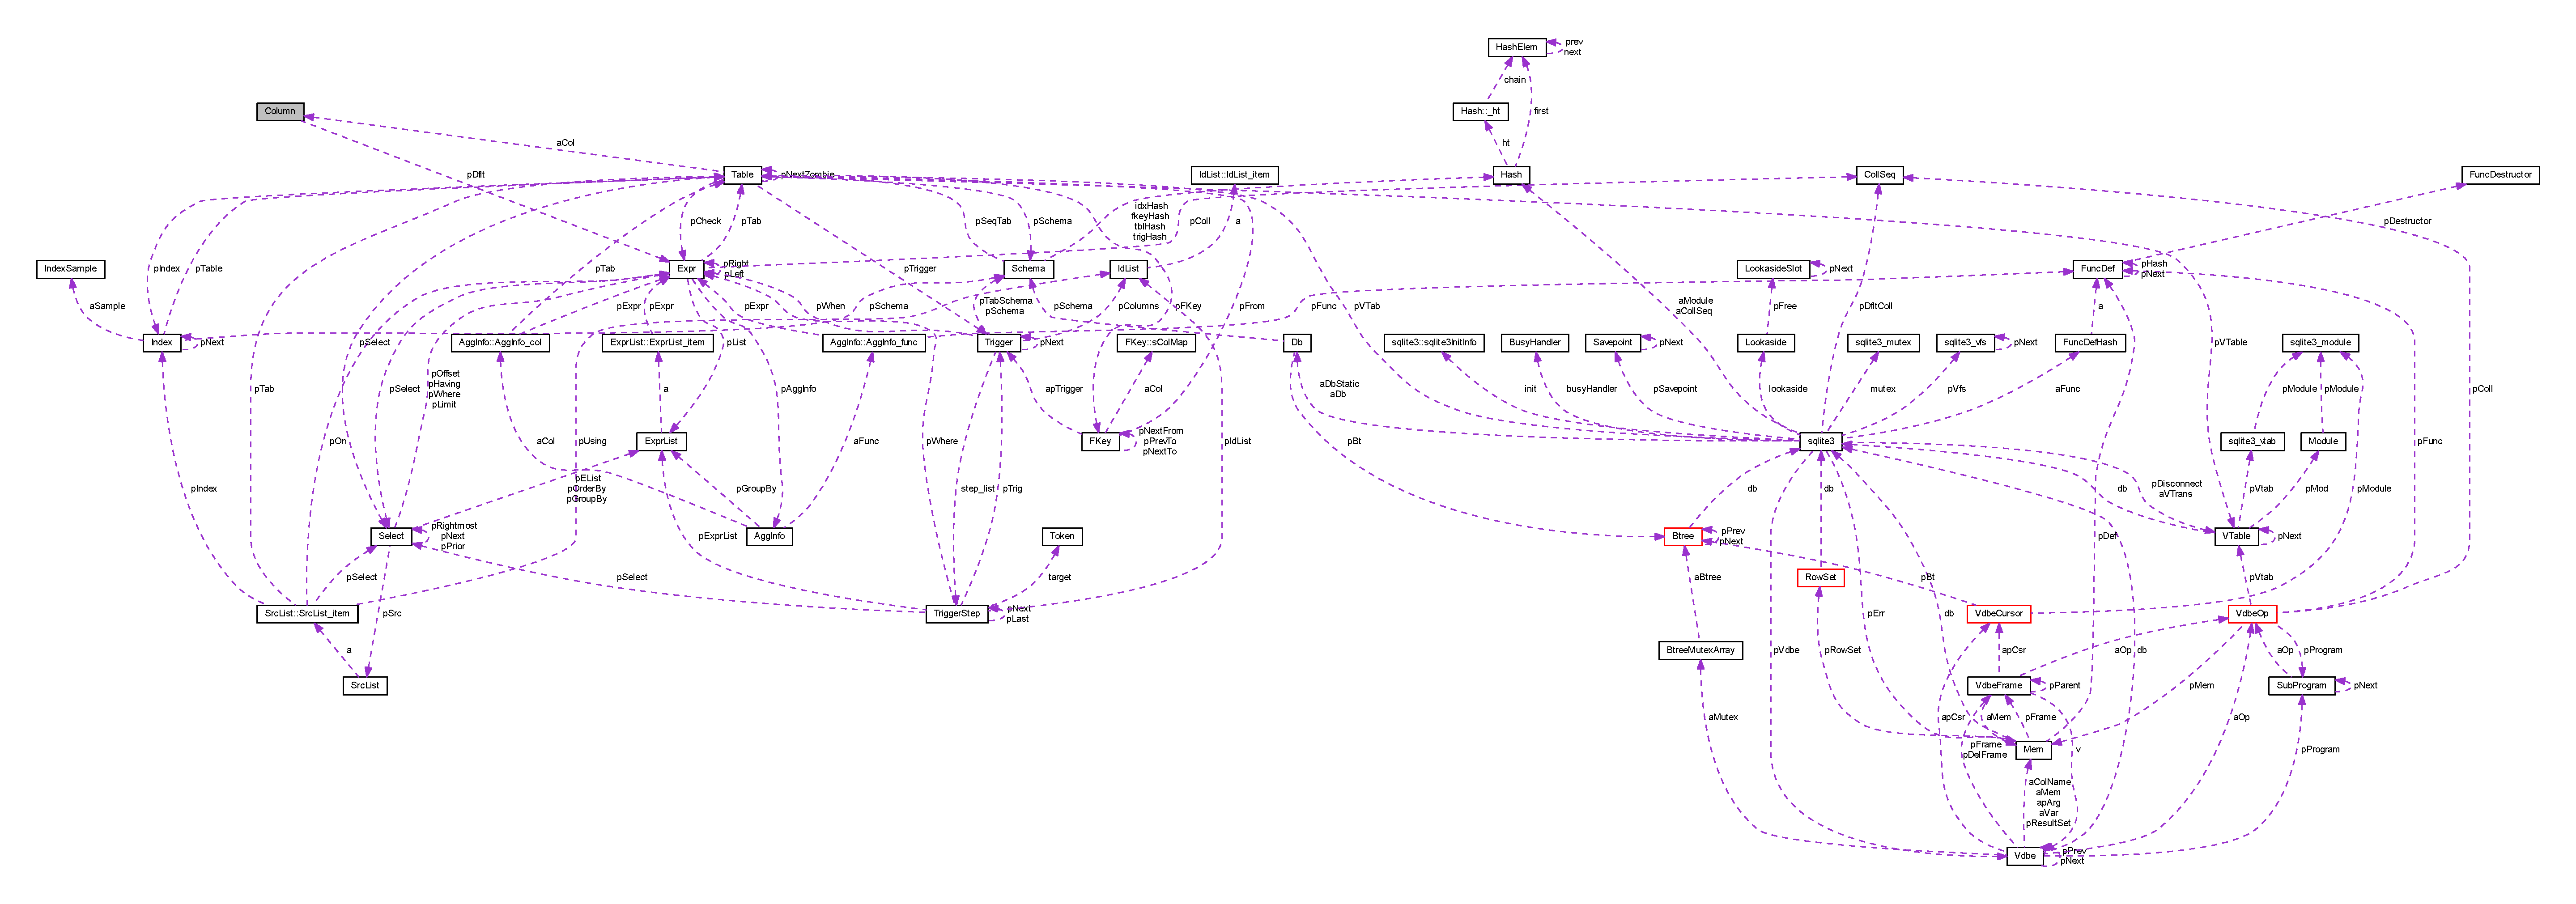
\includegraphics[width=350pt]{struct_column__coll__graph}
\end{center}
\end{figure}
\subsection*{Public Attributes}
\begin{DoxyCompactItemize}
\item 
\hypertarget{struct_column_a6450a4e9fde68b3a2d79425d826eccc3}{char $\ast$ {\bfseries z\-Name}}\label{struct_column_a6450a4e9fde68b3a2d79425d826eccc3}

\item 
\hypertarget{struct_column_ac4178f302df70048235660979f84ffe4}{\hyperlink{struct_expr}{Expr} $\ast$ {\bfseries p\-Dflt}}\label{struct_column_ac4178f302df70048235660979f84ffe4}

\item 
\hypertarget{struct_column_a88d29c685783cddfbd039e5674990f4b}{char $\ast$ {\bfseries z\-Dflt}}\label{struct_column_a88d29c685783cddfbd039e5674990f4b}

\item 
\hypertarget{struct_column_aef09f43479c4bd2d07f77d340020f95f}{char $\ast$ {\bfseries z\-Type}}\label{struct_column_aef09f43479c4bd2d07f77d340020f95f}

\item 
\hypertarget{struct_column_aa95909d5c77b321258622ed28d7b96eb}{char $\ast$ {\bfseries z\-Coll}}\label{struct_column_aa95909d5c77b321258622ed28d7b96eb}

\item 
\hypertarget{struct_column_a852e9a4c1c327a64d9b051dcafda3841}{u8 {\bfseries not\-Null}}\label{struct_column_a852e9a4c1c327a64d9b051dcafda3841}

\item 
\hypertarget{struct_column_a57a53c2c60925a1ce5fdfe8fa3ccd62a}{u8 {\bfseries is\-Prim\-Key}}\label{struct_column_a57a53c2c60925a1ce5fdfe8fa3ccd62a}

\item 
\hypertarget{struct_column_ac9d6fe31c45888cecaf3f5ad5b93bf23}{char {\bfseries affinity}}\label{struct_column_ac9d6fe31c45888cecaf3f5ad5b93bf23}

\item 
\hypertarget{struct_column_aafdb39efd9b21476415c5beeb5a8b180}{u8 {\bfseries is\-Hidden}}\label{struct_column_aafdb39efd9b21476415c5beeb5a8b180}

\end{DoxyCompactItemize}


The documentation for this struct was generated from the following file\-:\begin{DoxyCompactItemize}
\item 
C\-:/\-Users/\-Vitor/\-Desktop/\-Work\-Space/\-P\-R\-O\-J\-E\-T\-O\-\_\-\-F\-I\-N\-A\-L\-\_\-\-P\-O\-O/\-P\-R\-O\-J\-E\-T\-O\-\_\-\-D\-E\-V/\-P\-R\-O\-J\-E\-T\-O/\-Projeto\-\_\-codeblocks/sqlite3.\-c\end{DoxyCompactItemize}

\hypertarget{class_coment}{\section{Coment Class Reference}
\label{class_coment}\index{Coment@{Coment}}
}


Essa e a classe que repensenta os cometarios dos Usuarios nos posts no contexto do Sistema.  




{\ttfamily \#include $<$Entidades.\-h$>$}

\subsection*{Public Member Functions}
\begin{DoxyCompactItemize}
\item 
\hypertarget{class_coment_a578e61870997d13095a9daf39f2863bc}{\hyperlink{class_coment_a578e61870997d13095a9daf39f2863bc}{Coment} ()}\label{class_coment_a578e61870997d13095a9daf39f2863bc}

\begin{DoxyCompactList}\small\item\em Funcao contrutora da comentario quando nao ha paramentros, essa apenas inicia um novo comentario \par
 com todos os termos iquais a null. \end{DoxyCompactList}\item 
\hyperlink{class_coment_ae57275f77601a77eaa9b984589e025f2}{Coment} (\hyperlink{class_identify}{Identify}, \hyperlink{class_identify}{Identify}, \hyperlink{class_identify}{Identify}, \hyperlink{class_coment_text}{Coment\-Text}, \hyperlink{class_date}{Date})
\begin{DoxyCompactList}\small\item\em Funcao contrutora do \hyperlink{class_post}{Post} quando todos os termos sao passados no momento da criacao \par
 essa ira setar todos o termos passados. \end{DoxyCompactList}\item 
\hyperlink{class_identify}{Identify} \hyperlink{class_coment_a4006ae63196c19c5fb6feed70f6588ff}{get\-Author\-Identify} ()
\begin{DoxyCompactList}\small\item\em Pega o valor armazenado no campo identificador do author do comentario. \end{DoxyCompactList}\item 
void \hyperlink{class_coment_a29f4700734b5b9d50c17357876b3d96e}{set\-Author\-Identify} (\hyperlink{class_identify}{Identify})
\begin{DoxyCompactList}\small\item\em Da um set no valor do indetificador do auhthor do comentario. \end{DoxyCompactList}\item 
\hyperlink{class_identify}{Identify} \hyperlink{class_coment_a3fb57e3fdaf0e3c1e9d025af8e197e99}{get\-Post\-Identify} ()
\begin{DoxyCompactList}\small\item\em Pega o valor armazenado no campo indentificador do post do comentario. \end{DoxyCompactList}\item 
void \hyperlink{class_coment_a65bccaa5ff5ef75e22b19e41f1b2db08}{set\-Post\-Identify} (\hyperlink{class_identify}{Identify})
\begin{DoxyCompactList}\small\item\em Da um set no valor do campo do indentificador do post do comentario . \end{DoxyCompactList}\item 
\hyperlink{class_identify}{Identify} \hyperlink{class_coment_a6a57b7f20c9a0a4331f12b7058980b99}{get\-Coment\-Identify} ()
\begin{DoxyCompactList}\small\item\em Pega o valor armazenado no campo do indentificador unico do comentario. \end{DoxyCompactList}\item 
void \hyperlink{class_coment_ab980dae53d71c2c43d639482273e2032}{set\-Coment\-Identify} (\hyperlink{class_identify}{Identify})
\begin{DoxyCompactList}\small\item\em Da um set no valor do campo da avaliaçao. \end{DoxyCompactList}\item 
\hyperlink{class_coment_text}{Coment\-Text} \hyperlink{class_coment_a9d8b854216fe9e0c22d9daf58ac91d66}{get\-Coment\-Text} ()
\begin{DoxyCompactList}\small\item\em Pega o valor armazenado no campo do texto do comentario. \end{DoxyCompactList}\item 
void \hyperlink{class_coment_aee3806f744c85b8759d78caf327288a9}{set\-Coment\-Text} (\hyperlink{class_coment_text}{Coment\-Text})
\begin{DoxyCompactList}\small\item\em Da um set no valor do campo de texto do comentario. \end{DoxyCompactList}\item 
\hyperlink{class_date}{Date} \hyperlink{class_coment_a531f1b46ea41684e718b40ea48efde24}{get\-Date} ()
\begin{DoxyCompactList}\small\item\em Pega o valor armazenado no campo de data do comentario. \end{DoxyCompactList}\item 
void \hyperlink{class_coment_ad2faca7f8d5bac7538a9b5cde9642c46}{set\-Date} (\hyperlink{class_date}{Date})
\begin{DoxyCompactList}\small\item\em Da um set na data do comentario. \end{DoxyCompactList}\end{DoxyCompactItemize}


\subsection{Detailed Description}
Essa e a classe que repensenta os cometarios dos Usuarios nos posts no contexto do Sistema. 

\subsection{Constructor \& Destructor Documentation}
\hypertarget{class_coment_ae57275f77601a77eaa9b984589e025f2}{\index{Coment@{Coment}!Coment@{Coment}}
\index{Coment@{Coment}!Coment@{Coment}}
\subsubsection[{Coment}]{\setlength{\rightskip}{0pt plus 5cm}Coment\-::\-Coment (
\begin{DoxyParamCaption}
\item[{{\bf Identify}}]{author\-Identify, }
\item[{{\bf Identify}}]{post\-Identify, }
\item[{{\bf Identify}}]{coment\-Identify, }
\item[{{\bf Coment\-Text}}]{coment\-Text, }
\item[{{\bf Date}}]{date}
\end{DoxyParamCaption}
)}}\label{class_coment_ae57275f77601a77eaa9b984589e025f2}


Funcao contrutora do \hyperlink{class_post}{Post} quando todos os termos sao passados no momento da criacao \par
 essa ira setar todos o termos passados. 


\begin{DoxyParams}{Parameters}
{\em author\-Identify} & \-: o identificador do Usuario dono do comentario. \\
\hline
{\em post\-Identify} & \-: o identificador do post a que o comentario pertence. \\
\hline
{\em coment\-Identify} & \-: o identificador unico do comentario. \\
\hline
{\em coment\-Text} & \-: o texto do comentario. \\
\hline
{\em date} & \-: a data do comentario. \\
\hline
\end{DoxyParams}


Here is the call graph for this function\-:\nopagebreak
\begin{figure}[H]
\begin{center}
\leavevmode
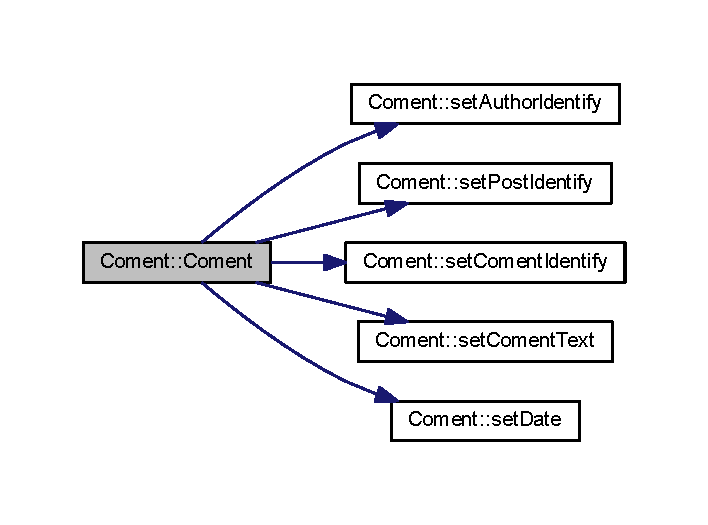
\includegraphics[width=340pt]{class_coment_ae57275f77601a77eaa9b984589e025f2_cgraph}
\end{center}
\end{figure}




\subsection{Member Function Documentation}
\hypertarget{class_coment_a4006ae63196c19c5fb6feed70f6588ff}{\index{Coment@{Coment}!get\-Author\-Identify@{get\-Author\-Identify}}
\index{get\-Author\-Identify@{get\-Author\-Identify}!Coment@{Coment}}
\subsubsection[{get\-Author\-Identify}]{\setlength{\rightskip}{0pt plus 5cm}{\bf Identify} Coment\-::get\-Author\-Identify (
\begin{DoxyParamCaption}
{}
\end{DoxyParamCaption}
)\hspace{0.3cm}{\ttfamily [inline]}}}\label{class_coment_a4006ae63196c19c5fb6feed70f6588ff}


Pega o valor armazenado no campo identificador do author do comentario. 

\begin{DoxyReturn}{Returns}
o identificador do author do comentario. 
\end{DoxyReturn}


Here is the caller graph for this function\-:\nopagebreak
\begin{figure}[H]
\begin{center}
\leavevmode
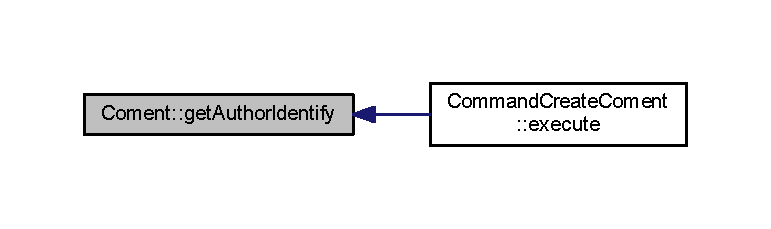
\includegraphics[width=350pt]{class_coment_a4006ae63196c19c5fb6feed70f6588ff_icgraph}
\end{center}
\end{figure}


\hypertarget{class_coment_a6a57b7f20c9a0a4331f12b7058980b99}{\index{Coment@{Coment}!get\-Coment\-Identify@{get\-Coment\-Identify}}
\index{get\-Coment\-Identify@{get\-Coment\-Identify}!Coment@{Coment}}
\subsubsection[{get\-Coment\-Identify}]{\setlength{\rightskip}{0pt plus 5cm}{\bf Identify} Coment\-::get\-Coment\-Identify (
\begin{DoxyParamCaption}
{}
\end{DoxyParamCaption}
)\hspace{0.3cm}{\ttfamily [inline]}}}\label{class_coment_a6a57b7f20c9a0a4331f12b7058980b99}


Pega o valor armazenado no campo do indentificador unico do comentario. 

\begin{DoxyReturn}{Returns}
o indetificador do comentario. 
\end{DoxyReturn}


Here is the caller graph for this function\-:\nopagebreak
\begin{figure}[H]
\begin{center}
\leavevmode
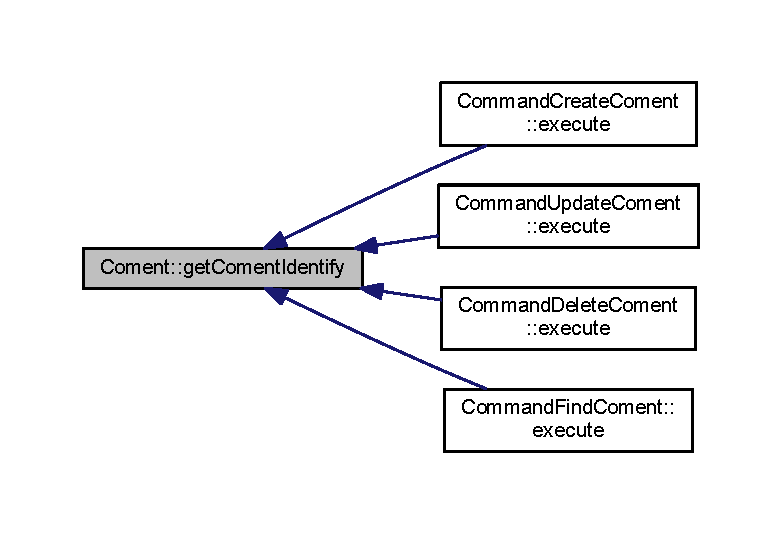
\includegraphics[width=350pt]{class_coment_a6a57b7f20c9a0a4331f12b7058980b99_icgraph}
\end{center}
\end{figure}


\hypertarget{class_coment_a9d8b854216fe9e0c22d9daf58ac91d66}{\index{Coment@{Coment}!get\-Coment\-Text@{get\-Coment\-Text}}
\index{get\-Coment\-Text@{get\-Coment\-Text}!Coment@{Coment}}
\subsubsection[{get\-Coment\-Text}]{\setlength{\rightskip}{0pt plus 5cm}{\bf Coment\-Text} Coment\-::get\-Coment\-Text (
\begin{DoxyParamCaption}
{}
\end{DoxyParamCaption}
)\hspace{0.3cm}{\ttfamily [inline]}}}\label{class_coment_a9d8b854216fe9e0c22d9daf58ac91d66}


Pega o valor armazenado no campo do texto do comentario. 

\begin{DoxyReturn}{Returns}
o texto do comentario. 
\end{DoxyReturn}


Here is the caller graph for this function\-:\nopagebreak
\begin{figure}[H]
\begin{center}
\leavevmode
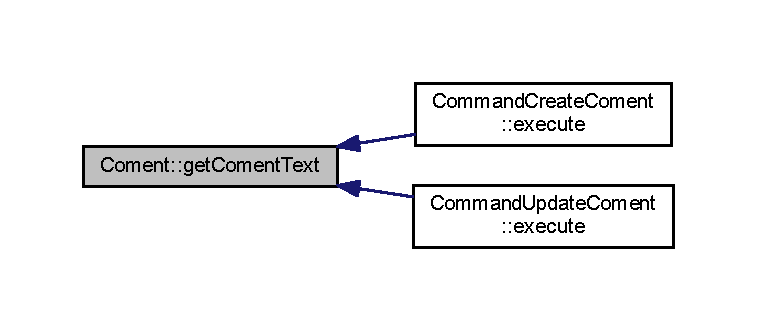
\includegraphics[width=350pt]{class_coment_a9d8b854216fe9e0c22d9daf58ac91d66_icgraph}
\end{center}
\end{figure}


\hypertarget{class_coment_a531f1b46ea41684e718b40ea48efde24}{\index{Coment@{Coment}!get\-Date@{get\-Date}}
\index{get\-Date@{get\-Date}!Coment@{Coment}}
\subsubsection[{get\-Date}]{\setlength{\rightskip}{0pt plus 5cm}{\bf Date} Coment\-::get\-Date (
\begin{DoxyParamCaption}
{}
\end{DoxyParamCaption}
)\hspace{0.3cm}{\ttfamily [inline]}}}\label{class_coment_a531f1b46ea41684e718b40ea48efde24}


Pega o valor armazenado no campo de data do comentario. 

\begin{DoxyReturn}{Returns}
a data do comentario. 
\end{DoxyReturn}


Here is the caller graph for this function\-:\nopagebreak
\begin{figure}[H]
\begin{center}
\leavevmode
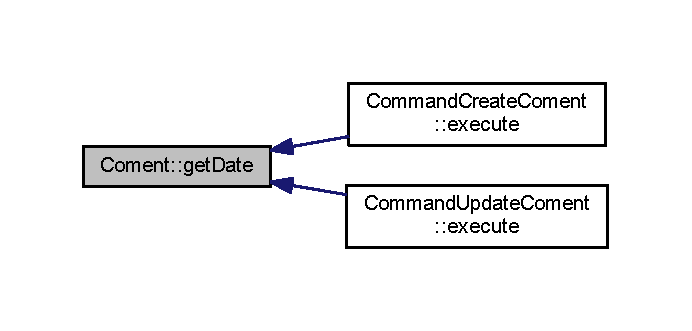
\includegraphics[width=332pt]{class_coment_a531f1b46ea41684e718b40ea48efde24_icgraph}
\end{center}
\end{figure}


\hypertarget{class_coment_a3fb57e3fdaf0e3c1e9d025af8e197e99}{\index{Coment@{Coment}!get\-Post\-Identify@{get\-Post\-Identify}}
\index{get\-Post\-Identify@{get\-Post\-Identify}!Coment@{Coment}}
\subsubsection[{get\-Post\-Identify}]{\setlength{\rightskip}{0pt plus 5cm}{\bf Identify} Coment\-::get\-Post\-Identify (
\begin{DoxyParamCaption}
{}
\end{DoxyParamCaption}
)\hspace{0.3cm}{\ttfamily [inline]}}}\label{class_coment_a3fb57e3fdaf0e3c1e9d025af8e197e99}


Pega o valor armazenado no campo indentificador do post do comentario. 

\begin{DoxyReturn}{Returns}
o indetificador do post a qual o comentario pertence. 
\end{DoxyReturn}


Here is the caller graph for this function\-:\nopagebreak
\begin{figure}[H]
\begin{center}
\leavevmode
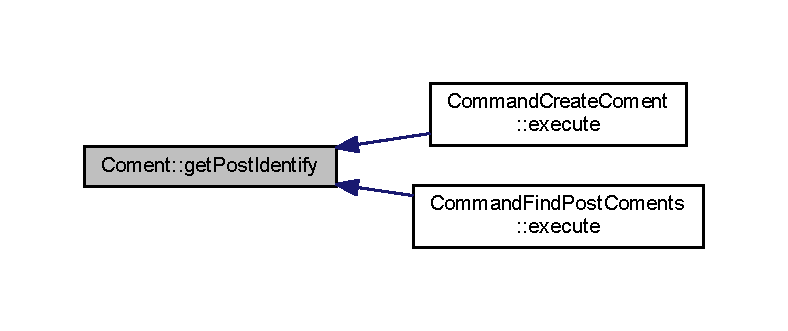
\includegraphics[width=350pt]{class_coment_a3fb57e3fdaf0e3c1e9d025af8e197e99_icgraph}
\end{center}
\end{figure}


\hypertarget{class_coment_a29f4700734b5b9d50c17357876b3d96e}{\index{Coment@{Coment}!set\-Author\-Identify@{set\-Author\-Identify}}
\index{set\-Author\-Identify@{set\-Author\-Identify}!Coment@{Coment}}
\subsubsection[{set\-Author\-Identify}]{\setlength{\rightskip}{0pt plus 5cm}void Coment\-::set\-Author\-Identify (
\begin{DoxyParamCaption}
\item[{{\bf Identify}}]{author\-Identify}
\end{DoxyParamCaption}
)\hspace{0.3cm}{\ttfamily [inline]}}}\label{class_coment_a29f4700734b5b9d50c17357876b3d96e}


Da um set no valor do indetificador do auhthor do comentario. 


\begin{DoxyParams}{Parameters}
{\em author\-Identify} & \-: o identificador do author do comentario. \\
\hline
\end{DoxyParams}


Here is the caller graph for this function\-:\nopagebreak
\begin{figure}[H]
\begin{center}
\leavevmode
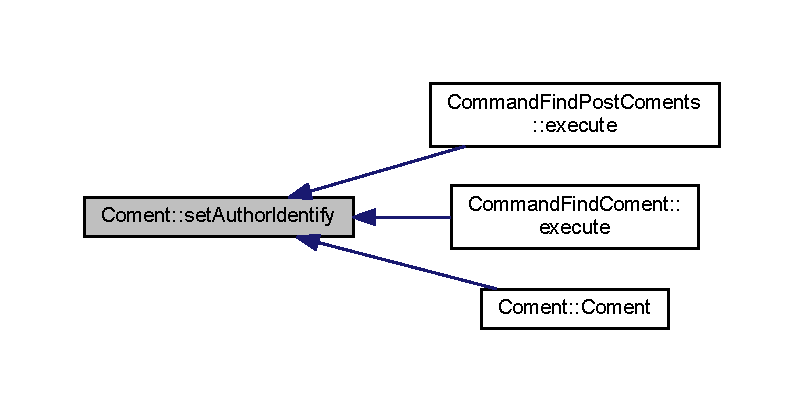
\includegraphics[width=350pt]{class_coment_a29f4700734b5b9d50c17357876b3d96e_icgraph}
\end{center}
\end{figure}


\hypertarget{class_coment_ab980dae53d71c2c43d639482273e2032}{\index{Coment@{Coment}!set\-Coment\-Identify@{set\-Coment\-Identify}}
\index{set\-Coment\-Identify@{set\-Coment\-Identify}!Coment@{Coment}}
\subsubsection[{set\-Coment\-Identify}]{\setlength{\rightskip}{0pt plus 5cm}void Coment\-::set\-Coment\-Identify (
\begin{DoxyParamCaption}
\item[{{\bf Identify}}]{coment\-Identify}
\end{DoxyParamCaption}
)\hspace{0.3cm}{\ttfamily [inline]}}}\label{class_coment_ab980dae53d71c2c43d639482273e2032}


Da um set no valor do campo da avaliaçao. 


\begin{DoxyParams}{Parameters}
{\em coment\-Identify} & \-: o identificador unico do comentario. \\
\hline
\end{DoxyParams}


Here is the caller graph for this function\-:\nopagebreak
\begin{figure}[H]
\begin{center}
\leavevmode
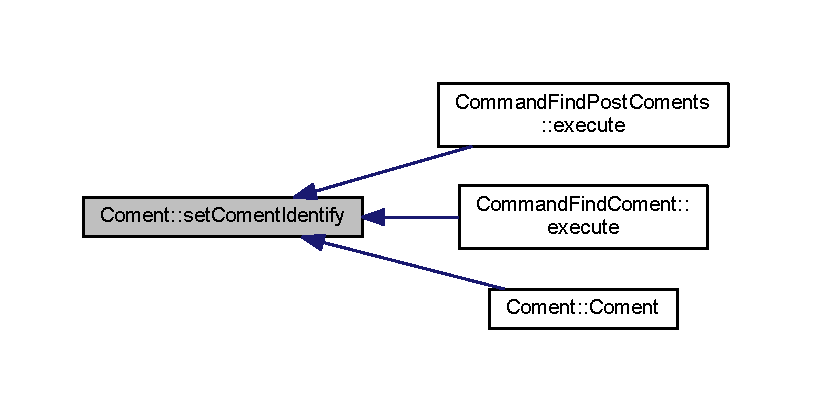
\includegraphics[width=350pt]{class_coment_ab980dae53d71c2c43d639482273e2032_icgraph}
\end{center}
\end{figure}


\hypertarget{class_coment_aee3806f744c85b8759d78caf327288a9}{\index{Coment@{Coment}!set\-Coment\-Text@{set\-Coment\-Text}}
\index{set\-Coment\-Text@{set\-Coment\-Text}!Coment@{Coment}}
\subsubsection[{set\-Coment\-Text}]{\setlength{\rightskip}{0pt plus 5cm}void Coment\-::set\-Coment\-Text (
\begin{DoxyParamCaption}
\item[{{\bf Coment\-Text}}]{coment\-Text}
\end{DoxyParamCaption}
)\hspace{0.3cm}{\ttfamily [inline]}}}\label{class_coment_aee3806f744c85b8759d78caf327288a9}


Da um set no valor do campo de texto do comentario. 


\begin{DoxyParams}{Parameters}
{\em coment\-Text} & \-: o texto do comentario. \\
\hline
\end{DoxyParams}


Here is the caller graph for this function\-:\nopagebreak
\begin{figure}[H]
\begin{center}
\leavevmode
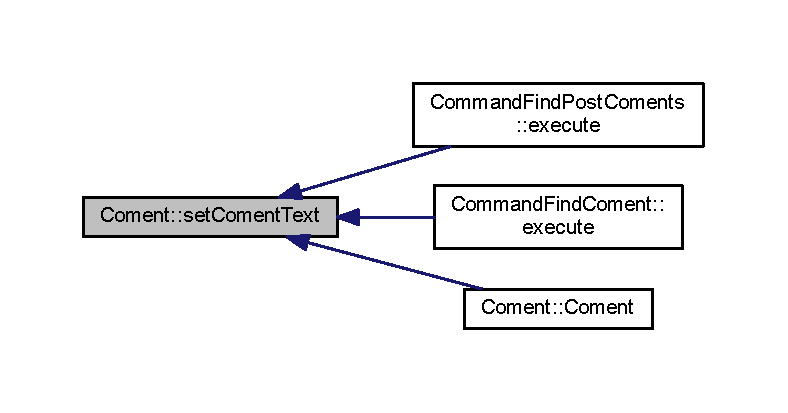
\includegraphics[width=350pt]{class_coment_aee3806f744c85b8759d78caf327288a9_icgraph}
\end{center}
\end{figure}


\hypertarget{class_coment_ad2faca7f8d5bac7538a9b5cde9642c46}{\index{Coment@{Coment}!set\-Date@{set\-Date}}
\index{set\-Date@{set\-Date}!Coment@{Coment}}
\subsubsection[{set\-Date}]{\setlength{\rightskip}{0pt plus 5cm}void Coment\-::set\-Date (
\begin{DoxyParamCaption}
\item[{{\bf Date}}]{date}
\end{DoxyParamCaption}
)\hspace{0.3cm}{\ttfamily [inline]}}}\label{class_coment_ad2faca7f8d5bac7538a9b5cde9642c46}


Da um set na data do comentario. 


\begin{DoxyParams}{Parameters}
{\em date} & \-: a data do comentario. \\
\hline
\end{DoxyParams}


Here is the caller graph for this function\-:\nopagebreak
\begin{figure}[H]
\begin{center}
\leavevmode
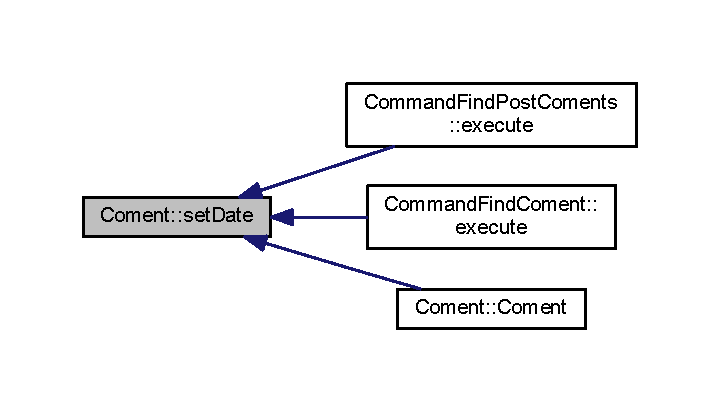
\includegraphics[width=346pt]{class_coment_ad2faca7f8d5bac7538a9b5cde9642c46_icgraph}
\end{center}
\end{figure}


\hypertarget{class_coment_a65bccaa5ff5ef75e22b19e41f1b2db08}{\index{Coment@{Coment}!set\-Post\-Identify@{set\-Post\-Identify}}
\index{set\-Post\-Identify@{set\-Post\-Identify}!Coment@{Coment}}
\subsubsection[{set\-Post\-Identify}]{\setlength{\rightskip}{0pt plus 5cm}void Coment\-::set\-Post\-Identify (
\begin{DoxyParamCaption}
\item[{{\bf Identify}}]{post\-Identify}
\end{DoxyParamCaption}
)\hspace{0.3cm}{\ttfamily [inline]}}}\label{class_coment_a65bccaa5ff5ef75e22b19e41f1b2db08}


Da um set no valor do campo do indentificador do post do comentario . 


\begin{DoxyParams}{Parameters}
{\em post\-Identify} & \-: o indentificador do post do comentariot. \\
\hline
\end{DoxyParams}


Here is the caller graph for this function\-:\nopagebreak
\begin{figure}[H]
\begin{center}
\leavevmode
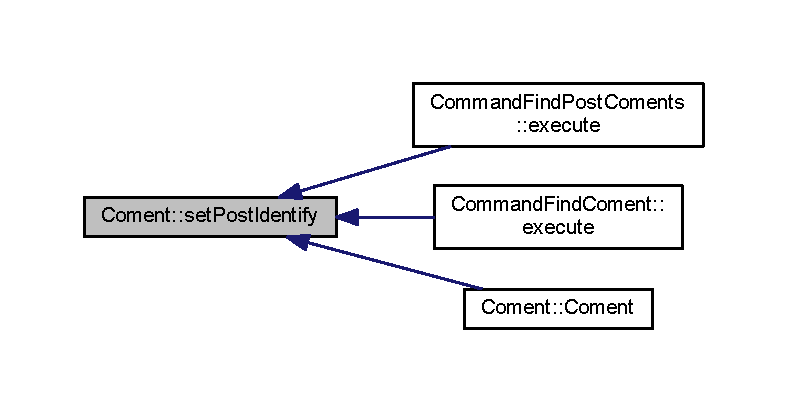
\includegraphics[width=350pt]{class_coment_a65bccaa5ff5ef75e22b19e41f1b2db08_icgraph}
\end{center}
\end{figure}




The documentation for this class was generated from the following files\-:\begin{DoxyCompactItemize}
\item 
C\-:/\-Users/\-Vitor/\-Desktop/\-Work\-Space/\-P\-R\-O\-J\-E\-T\-O\-\_\-\-F\-I\-N\-A\-L\-\_\-\-P\-O\-O/\-P\-R\-O\-J\-E\-T\-O\-\_\-\-D\-E\-V/\-P\-R\-O\-J\-E\-T\-O/\-Projeto\-\_\-codeblocks/\hyperlink{_entidades_8h}{Entidades.\-h}\item 
C\-:/\-Users/\-Vitor/\-Desktop/\-Work\-Space/\-P\-R\-O\-J\-E\-T\-O\-\_\-\-F\-I\-N\-A\-L\-\_\-\-P\-O\-O/\-P\-R\-O\-J\-E\-T\-O\-\_\-\-D\-E\-V/\-P\-R\-O\-J\-E\-T\-O/\-Projeto\-\_\-codeblocks/Entidades.\-cpp\end{DoxyCompactItemize}

\hypertarget{class_coment_command}{\section{Coment\-Command Class Reference}
\label{class_coment_command}\index{Coment\-Command@{Coment\-Command}}
}


Classe que possui todos os comandos que podem ser realizados para um post.  




{\ttfamily \#include $<$Comand.\-h$>$}



Inheritance diagram for Coment\-Command\-:\nopagebreak
\begin{figure}[H]
\begin{center}
\leavevmode
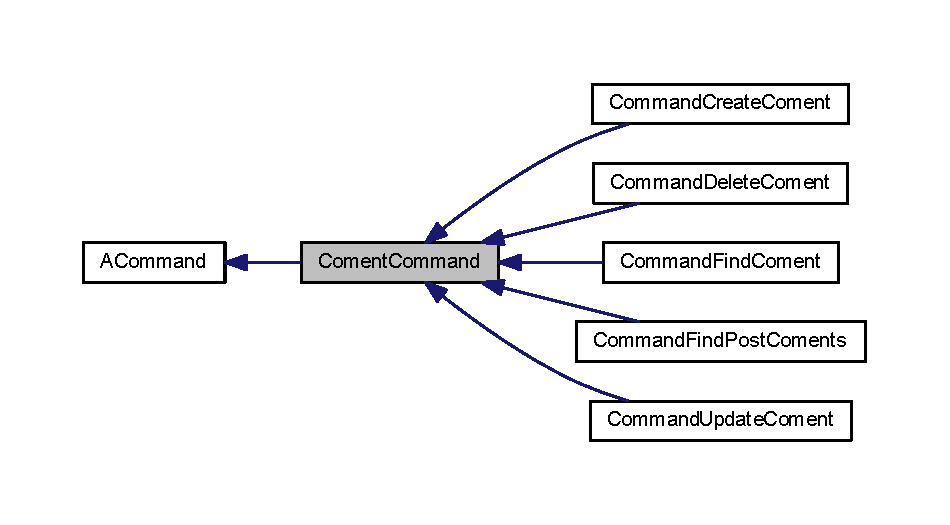
\includegraphics[width=350pt]{class_coment_command__inherit__graph}
\end{center}
\end{figure}


Collaboration diagram for Coment\-Command\-:\nopagebreak
\begin{figure}[H]
\begin{center}
\leavevmode
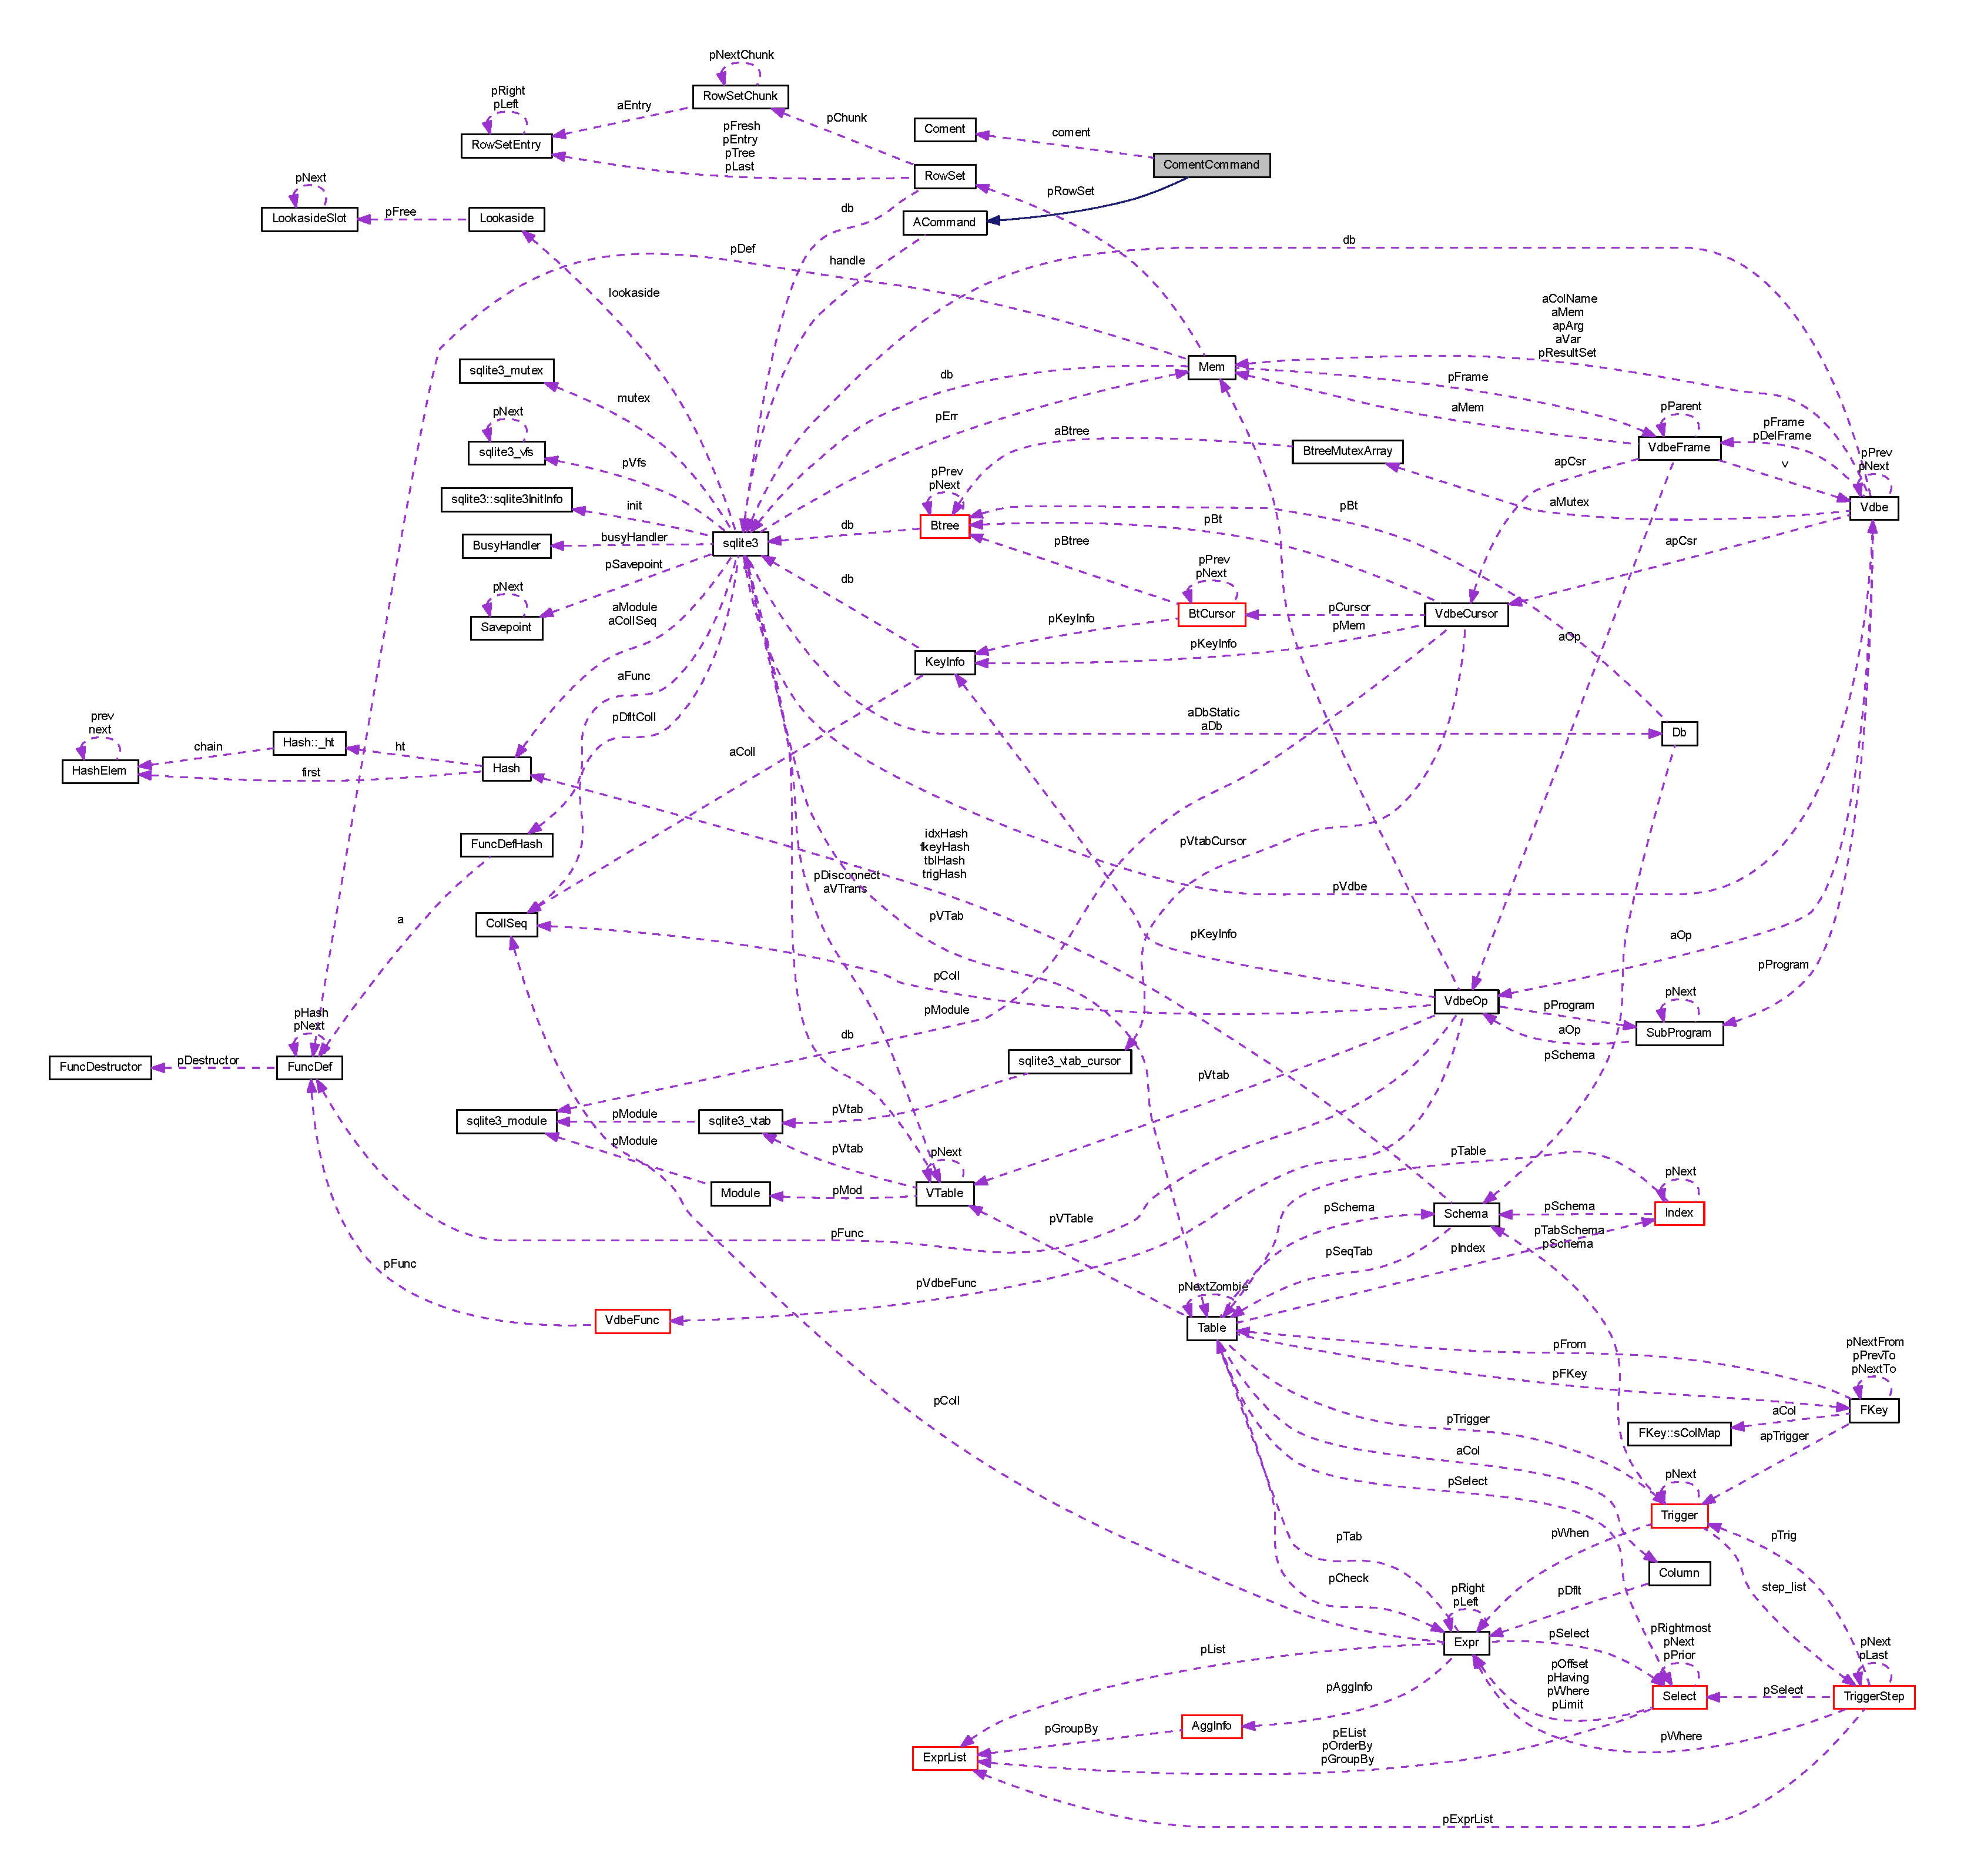
\includegraphics[width=350pt]{class_coment_command__coll__graph}
\end{center}
\end{figure}
\subsection*{Public Member Functions}
\begin{DoxyCompactItemize}
\item 
void \hyperlink{class_coment_command_a7dcbcf61c4dcbb080881535ba1093711}{set\-Coment} (\hyperlink{class_coment}{Coment} \hyperlink{class_coment_command_aeeadc825656bf9e76ce0ea3f721749e0}{coment})
\begin{DoxyCompactList}\small\item\em Método responsável por adicionar um comentário no banco de dados. \end{DoxyCompactList}\item 
\hypertarget{class_coment_command_a4ce5a7ad5abb44fbe6951dd10c576f67}{\hyperlink{class_coment}{Coment} \hyperlink{class_coment_command_a4ce5a7ad5abb44fbe6951dd10c576f67}{get\-Coment} ()}\label{class_coment_command_a4ce5a7ad5abb44fbe6951dd10c576f67}

\begin{DoxyCompactList}\small\item\em Método responsável por adicionar um comentário no banco de dados. \end{DoxyCompactList}\item 
\hypertarget{class_coment_command_a2e31acac5682b142fdff5dc5ebee7e93}{list$<$ \hyperlink{class_coment}{Coment} $>$ \hyperlink{class_coment_command_a2e31acac5682b142fdff5dc5ebee7e93}{get\-List} ()}\label{class_coment_command_a2e31acac5682b142fdff5dc5ebee7e93}

\begin{DoxyCompactList}\small\item\em Método responsável por listar os comentários de um post do banco de dados. \end{DoxyCompactList}\end{DoxyCompactItemize}
\subsection*{Protected Attributes}
\begin{DoxyCompactItemize}
\item 
\hyperlink{class_coment}{Coment} \hyperlink{class_coment_command_aeeadc825656bf9e76ce0ea3f721749e0}{coment}
\item 
std\-::list$<$ \hyperlink{class_coment}{Coment} $>$ \hyperlink{class_coment_command_ad0ae90b7aacb5dc53857351855845488}{coments}
\end{DoxyCompactItemize}
\subsection*{Additional Inherited Members}


\subsection{Detailed Description}
Classe que possui todos os comandos que podem ser realizados para um post. 

\subsection{Member Function Documentation}
\hypertarget{class_coment_command_a7dcbcf61c4dcbb080881535ba1093711}{\index{Coment\-Command@{Coment\-Command}!set\-Coment@{set\-Coment}}
\index{set\-Coment@{set\-Coment}!ComentCommand@{Coment\-Command}}
\subsubsection[{set\-Coment}]{\setlength{\rightskip}{0pt plus 5cm}void Coment\-Command\-::set\-Coment (
\begin{DoxyParamCaption}
\item[{{\bf Coment}}]{coment}
\end{DoxyParamCaption}
)\hspace{0.3cm}{\ttfamily [inline]}}}\label{class_coment_command_a7dcbcf61c4dcbb080881535ba1093711}


Método responsável por adicionar um comentário no banco de dados. 


\begin{DoxyParams}{Parameters}
{\em \hyperlink{class_coment}{Coment}} & = Objeto de um comentário \\
\hline
\end{DoxyParams}


Here is the caller graph for this function\-:\nopagebreak
\begin{figure}[H]
\begin{center}
\leavevmode
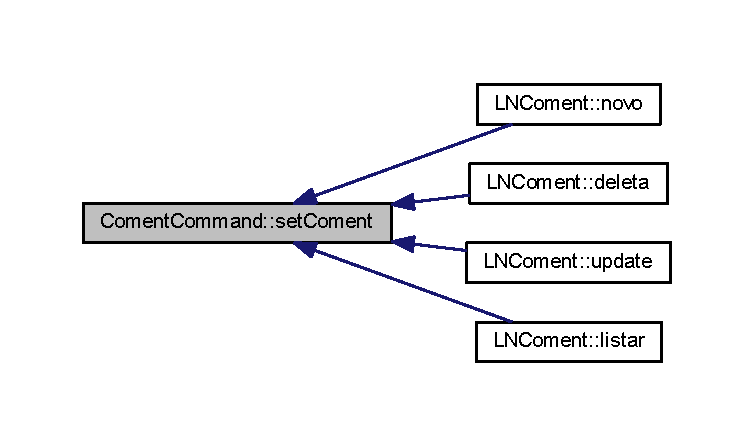
\includegraphics[width=350pt]{class_coment_command_a7dcbcf61c4dcbb080881535ba1093711_icgraph}
\end{center}
\end{figure}




\subsection{Member Data Documentation}
\hypertarget{class_coment_command_aeeadc825656bf9e76ce0ea3f721749e0}{\index{Coment\-Command@{Coment\-Command}!coment@{coment}}
\index{coment@{coment}!ComentCommand@{Coment\-Command}}
\subsubsection[{coment}]{\setlength{\rightskip}{0pt plus 5cm}{\bf Coment} Coment\-Command\-::coment\hspace{0.3cm}{\ttfamily [protected]}}}\label{class_coment_command_aeeadc825656bf9e76ce0ea3f721749e0}
Variavel que contém o objeto de um comentário \hypertarget{class_coment_command_ad0ae90b7aacb5dc53857351855845488}{\index{Coment\-Command@{Coment\-Command}!coments@{coments}}
\index{coments@{coments}!ComentCommand@{Coment\-Command}}
\subsubsection[{coments}]{\setlength{\rightskip}{0pt plus 5cm}std\-::list$<${\bf Coment}$>$ Coment\-Command\-::coments\hspace{0.3cm}{\ttfamily [protected]}}}\label{class_coment_command_ad0ae90b7aacb5dc53857351855845488}
Variavel que contém uma lista de objetos de comentários 

The documentation for this class was generated from the following file\-:\begin{DoxyCompactItemize}
\item 
C\-:/\-Users/\-Vitor/\-Desktop/\-Work\-Space/\-P\-R\-O\-J\-E\-T\-O\-\_\-\-F\-I\-N\-A\-L\-\_\-\-P\-O\-O/\-P\-R\-O\-J\-E\-T\-O\-\_\-\-D\-E\-V/\-P\-R\-O\-J\-E\-T\-O/\-Projeto\-\_\-codeblocks/Comand.\-h\end{DoxyCompactItemize}

\hypertarget{class_coment_controler}{\section{Coment\-Controler Class Reference}
\label{class_coment_controler}\index{Coment\-Controler@{Coment\-Controler}}
}


Essa é a classe que cria a interface de comandos de comentário.  




{\ttfamily \#include $<$Inter\-Usu.\-h$>$}



Inheritance diagram for Coment\-Controler\-:
\nopagebreak
\begin{figure}[H]
\begin{center}
\leavevmode
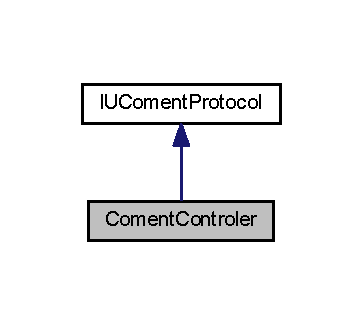
\includegraphics[width=174pt]{class_coment_controler__inherit__graph}
\end{center}
\end{figure}


Collaboration diagram for Coment\-Controler\-:
\nopagebreak
\begin{figure}[H]
\begin{center}
\leavevmode
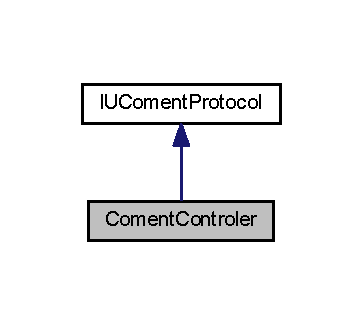
\includegraphics[width=174pt]{class_coment_controler__coll__graph}
\end{center}
\end{figure}
\subsection*{Public Member Functions}
\begin{DoxyCompactItemize}
\item 
\hypertarget{class_coment_controler_a3717c8a74f5091b6af228388b15f8259}{void \hyperlink{class_coment_controler_a3717c8a74f5091b6af228388b15f8259}{exec} ()}\label{class_coment_controler_a3717c8a74f5091b6af228388b15f8259}

\begin{DoxyCompactList}\small\item\em Método responsável por inicializar a interface. \end{DoxyCompactList}\item 
\hypertarget{class_coment_controler_a6438b12dbad045d3437978e6fd875159}{void \hyperlink{class_coment_controler_a6438b12dbad045d3437978e6fd875159}{set\-User} (User $\ast$)}\label{class_coment_controler_a6438b12dbad045d3437978e6fd875159}

\begin{DoxyCompactList}\small\item\em Método responsável por setar usuario. \end{DoxyCompactList}\item 
\hypertarget{class_coment_controler_a24dea8665cd60a397c83527f0b179210}{void \hyperlink{class_coment_controler_a24dea8665cd60a397c83527f0b179210}{set\-Post} (Post $\ast$)}\label{class_coment_controler_a24dea8665cd60a397c83527f0b179210}

\begin{DoxyCompactList}\small\item\em Método responsável por setar post. \end{DoxyCompactList}\item 
\hypertarget{class_coment_controler_a297cdd6c8e43c69d092d78f2db56645a}{void \hyperlink{class_coment_controler_a297cdd6c8e43c69d092d78f2db56645a}{set\-Logic\-Protocol} (Coment\-Protocol $\ast$)}\label{class_coment_controler_a297cdd6c8e43c69d092d78f2db56645a}

\begin{DoxyCompactList}\small\item\em Método responsável por setar a logica. \end{DoxyCompactList}\end{DoxyCompactItemize}


\subsection{Detailed Description}
Essa é a classe que cria a interface de comandos de comentário. 

The documentation for this class was generated from the following files\-:\begin{DoxyCompactItemize}
\item 
Inter\-Usu.\-h\item 
Inter\-Usu.\-cpp\end{DoxyCompactItemize}

\hypertarget{class_coment_protocol}{\section{Coment\-Protocol Class Reference}
\label{class_coment_protocol}\index{Coment\-Protocol@{Coment\-Protocol}}
}


Inheritance diagram for Coment\-Protocol\-:\nopagebreak
\begin{figure}[H]
\begin{center}
\leavevmode
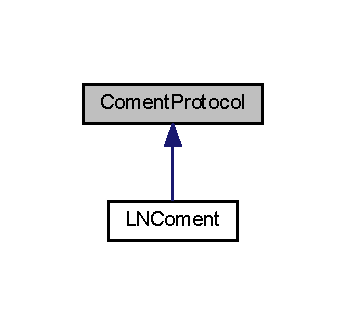
\includegraphics[width=166pt]{class_coment_protocol__inherit__graph}
\end{center}
\end{figure}
\subsection*{Public Member Functions}
\begin{DoxyCompactItemize}
\item 
\hypertarget{class_coment_protocol_a96c2e0cb9eb4fdbf5a7eae853b6546df}{virtual void {\bfseries novo} (\hyperlink{class_coment}{Coment})=0}\label{class_coment_protocol_a96c2e0cb9eb4fdbf5a7eae853b6546df}

\item 
\hypertarget{class_coment_protocol_a5a1cc6af2c1a52b489e6897070e4183a}{virtual void {\bfseries update} (\hyperlink{class_coment}{Coment})=0}\label{class_coment_protocol_a5a1cc6af2c1a52b489e6897070e4183a}

\item 
\hypertarget{class_coment_protocol_a466292c4e836394ce7a46a9b86412cae}{virtual void {\bfseries deleta} (\hyperlink{class_coment}{Coment})=0}\label{class_coment_protocol_a466292c4e836394ce7a46a9b86412cae}

\item 
\hypertarget{class_coment_protocol_a3a1f008a4638d4d1505b416d7e866158}{virtual \hyperlink{class_coment}{Coment} {\bfseries pegar} (\hyperlink{class_coment}{Coment})=0}\label{class_coment_protocol_a3a1f008a4638d4d1505b416d7e866158}

\item 
\hypertarget{class_coment_protocol_af626d6d87a2586d33d8fdfbab674ea1a}{virtual list$<$ \hyperlink{class_coment}{Coment} $>$ {\bfseries listar} (\hyperlink{class_coment}{Coment})=0}\label{class_coment_protocol_af626d6d87a2586d33d8fdfbab674ea1a}

\item 
\hypertarget{class_coment_protocol_a282b789ce1d561b29a3eb68af1de7296}{virtual void {\bfseries set\-Percistence} (\hyperlink{class_percistence_protocol}{Percistence\-Protocol} $\ast$)=0}\label{class_coment_protocol_a282b789ce1d561b29a3eb68af1de7296}

\end{DoxyCompactItemize}


The documentation for this class was generated from the following file\-:\begin{DoxyCompactItemize}
\item 
C\-:/\-Users/\-Vitor/\-Desktop/\-Work\-Space/\-P\-R\-O\-J\-E\-T\-O\-\_\-\-F\-I\-N\-A\-L\-\_\-\-P\-O\-O/\-P\-R\-O\-J\-E\-T\-O\-\_\-\-D\-E\-V/\-P\-R\-O\-J\-E\-T\-O/\-Projeto\-\_\-codeblocks/\hyperlink{_protocolo_l_n_8h}{Protocolo\-L\-N.\-h}\end{DoxyCompactItemize}

\hypertarget{class_coment_text}{\section{Coment\-Text Class Reference}
\label{class_coment_text}\index{Coment\-Text@{Coment\-Text}}
}


Essa e a classe responsavel por represnetar os textos do comentarios no contexto do sistema.  




{\ttfamily \#include $<$Tipos\-Basicos.\-h$>$}



Inheritance diagram for Coment\-Text\-:\nopagebreak
\begin{figure}[H]
\begin{center}
\leavevmode
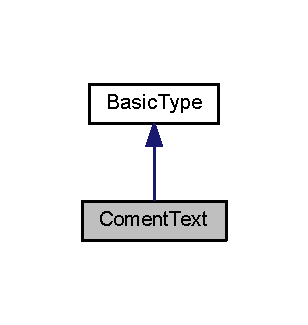
\includegraphics[width=148pt]{class_coment_text__inherit__graph}
\end{center}
\end{figure}


Collaboration diagram for Coment\-Text\-:\nopagebreak
\begin{figure}[H]
\begin{center}
\leavevmode
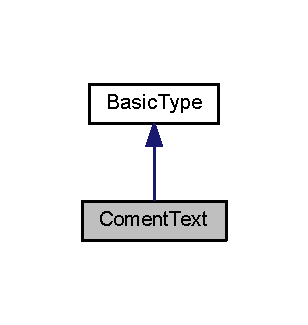
\includegraphics[width=148pt]{class_coment_text__coll__graph}
\end{center}
\end{figure}
\subsection*{Public Member Functions}
\begin{DoxyCompactItemize}
\item 
\hypertarget{class_coment_text_a7c8c9aa482e3f4a2b9e4aa194b946814}{\hyperlink{class_coment_text_a7c8c9aa482e3f4a2b9e4aa194b946814}{Coment\-Text} ()  throw (invalid\-\_\-argument)}\label{class_coment_text_a7c8c9aa482e3f4a2b9e4aa194b946814}

\begin{DoxyCompactList}\small\item\em Funcao contrutora do Cment\-Text quando nao ha paramentros, essa apenas inicia um texto de comentario vazio. 
\begin{DoxyExceptions}{Exceptions}
{\em std\-::invalid\-\_\-argument} & quando a classe nao pode ser vazia. \\
\hline
\end{DoxyExceptions}
\end{DoxyCompactList}\item 
\hyperlink{class_coment_text_a9e8f0908ebb65c6debeaf1ccfde2041d}{Coment\-Text} (const string \&\hyperlink{class_basic_type_af9b2c5cc32647df01083a6802e913dbf}{value})  throw (invalid\-\_\-argument)
\begin{DoxyCompactList}\small\item\em Funcao contrutora do \hyperlink{class_coment_text}{Coment\-Text} quando todos os termos sao passados no momento da criacao \par
 essa ira setar todos o termos passados. \end{DoxyCompactList}\end{DoxyCompactItemize}
\subsection*{Additional Inherited Members}


\subsection{Detailed Description}
Essa e a classe responsavel por represnetar os textos do comentarios no contexto do sistema. 

\subsection{Constructor \& Destructor Documentation}
\hypertarget{class_coment_text_a9e8f0908ebb65c6debeaf1ccfde2041d}{\index{Coment\-Text@{Coment\-Text}!Coment\-Text@{Coment\-Text}}
\index{Coment\-Text@{Coment\-Text}!ComentText@{Coment\-Text}}
\subsubsection[{Coment\-Text}]{\setlength{\rightskip}{0pt plus 5cm}Coment\-Text\-::\-Coment\-Text (
\begin{DoxyParamCaption}
\item[{const string \&}]{value}
\end{DoxyParamCaption}
)  throw (invalid\-\_\-argument)}}\label{class_coment_text_a9e8f0908ebb65c6debeaf1ccfde2041d}


Funcao contrutora do \hyperlink{class_coment_text}{Coment\-Text} quando todos os termos sao passados no momento da criacao \par
 essa ira setar todos o termos passados. 


\begin{DoxyParams}{Parameters}
{\em value} & \-: o texto do comentario. \\
\hline
\end{DoxyParams}

\begin{DoxyExceptions}{Exceptions}
{\em std\-::invalid\-\_\-argument} & o argumeto e invalido. \\
\hline
\end{DoxyExceptions}


The documentation for this class was generated from the following files\-:\begin{DoxyCompactItemize}
\item 
C\-:/\-Users/\-Vitor/\-Desktop/\-Work\-Space/\-P\-R\-O\-J\-E\-T\-O\-\_\-\-F\-I\-N\-A\-L\-\_\-\-P\-O\-O/\-P\-R\-O\-J\-E\-T\-O\-\_\-\-D\-E\-V/\-P\-R\-O\-J\-E\-T\-O/\-Projeto\-\_\-codeblocks/\hyperlink{_tipos_basicos_8h}{Tipos\-Basicos.\-h}\item 
C\-:/\-Users/\-Vitor/\-Desktop/\-Work\-Space/\-P\-R\-O\-J\-E\-T\-O\-\_\-\-F\-I\-N\-A\-L\-\_\-\-P\-O\-O/\-P\-R\-O\-J\-E\-T\-O\-\_\-\-D\-E\-V/\-P\-R\-O\-J\-E\-T\-O/\-Projeto\-\_\-codeblocks/Tipos\-Basicos.\-cpp\end{DoxyCompactItemize}

\hypertarget{class_command_create_coment}{\section{Command\-Create\-Coment Class Reference}
\label{class_command_create_coment}\index{Command\-Create\-Coment@{Command\-Create\-Coment}}
}


Classe que irá procurar se já existe um id,igual ao do objeto, no bd, se esse não existir irá adicionar o obj.  




{\ttfamily \#include $<$Comand.\-h$>$}



Inheritance diagram for Command\-Create\-Coment\-:\nopagebreak
\begin{figure}[H]
\begin{center}
\leavevmode
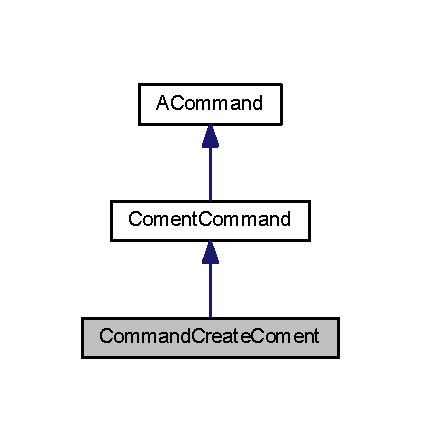
\includegraphics[width=202pt]{class_command_create_coment__inherit__graph}
\end{center}
\end{figure}


Collaboration diagram for Command\-Create\-Coment\-:\nopagebreak
\begin{figure}[H]
\begin{center}
\leavevmode
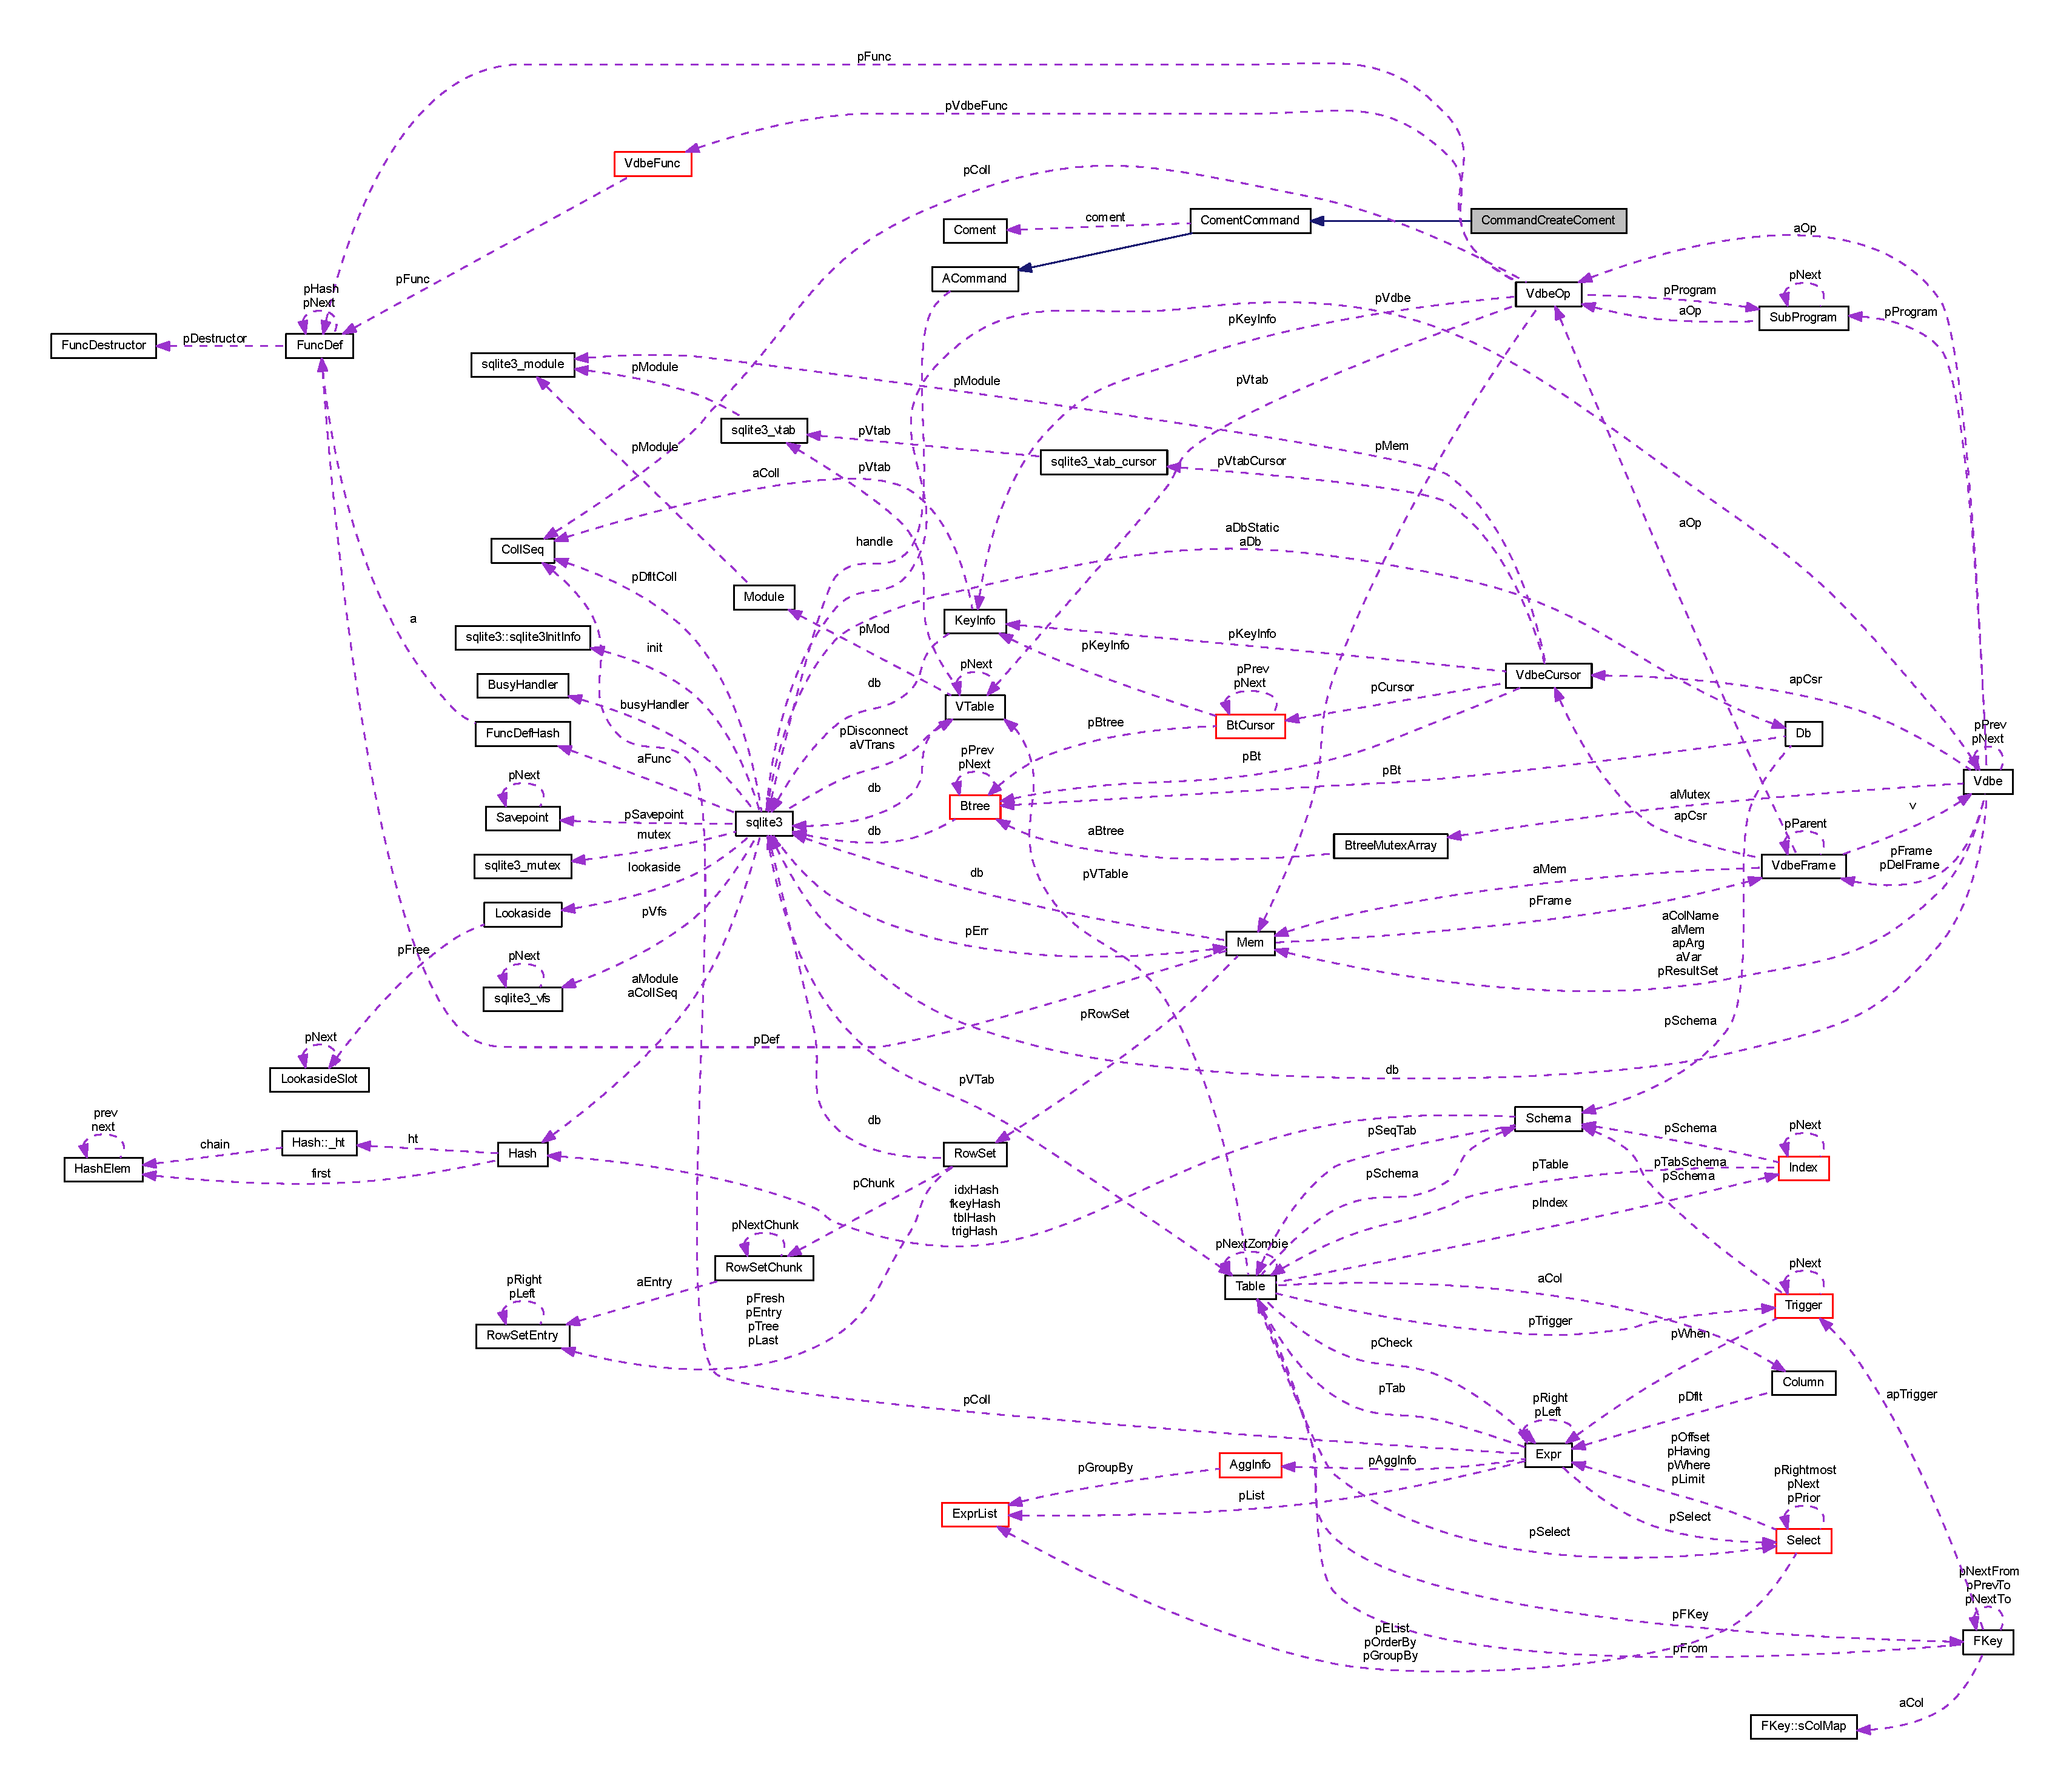
\includegraphics[width=350pt]{class_command_create_coment__coll__graph}
\end{center}
\end{figure}
\subsection*{Public Member Functions}
\begin{DoxyCompactItemize}
\item 
void \hyperlink{class_command_create_coment_aaefce07a8f35b3e236edc0ef8d68b756}{execute} ()
\begin{DoxyCompactList}\small\item\em Método responsável por iniciar a execução da classe. \end{DoxyCompactList}\end{DoxyCompactItemize}
\subsection*{Additional Inherited Members}


\subsection{Detailed Description}
Classe que irá procurar se já existe um id,igual ao do objeto, no bd, se esse não existir irá adicionar o obj. 

\subsection{Member Function Documentation}
\hypertarget{class_command_create_coment_aaefce07a8f35b3e236edc0ef8d68b756}{\index{Command\-Create\-Coment@{Command\-Create\-Coment}!execute@{execute}}
\index{execute@{execute}!CommandCreateComent@{Command\-Create\-Coment}}
\subsubsection[{execute}]{\setlength{\rightskip}{0pt plus 5cm}void Command\-Create\-Coment\-::execute (
\begin{DoxyParamCaption}
{}
\end{DoxyParamCaption}
)\hspace{0.3cm}{\ttfamily [virtual]}}}\label{class_command_create_coment_aaefce07a8f35b3e236edc0ef8d68b756}


Método responsável por iniciar a execução da classe. 

I\-D já existe 

Implements \hyperlink{class_a_command_a94c6a1d25eb0427389e15450019ebad8}{A\-Command}.



Here is the call graph for this function\-:\nopagebreak
\begin{figure}[H]
\begin{center}
\leavevmode
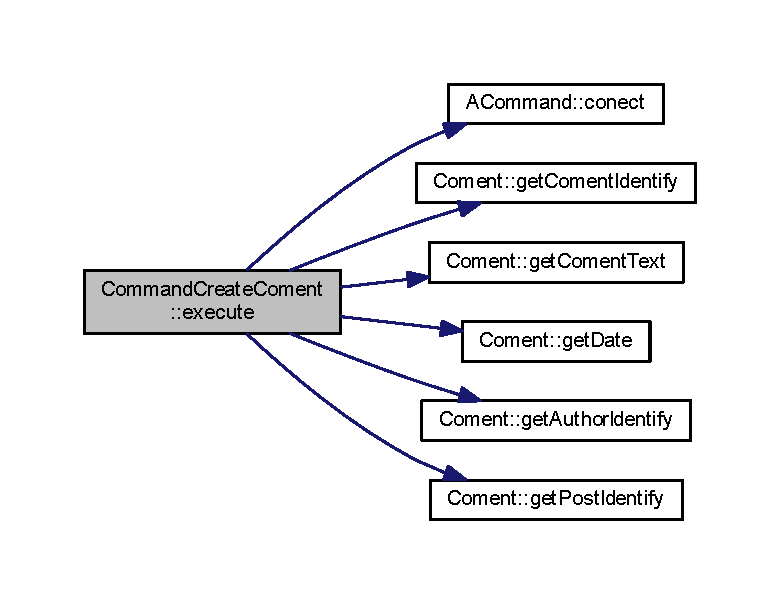
\includegraphics[width=344pt]{class_command_create_coment_aaefce07a8f35b3e236edc0ef8d68b756_cgraph}
\end{center}
\end{figure}




The documentation for this class was generated from the following files\-:\begin{DoxyCompactItemize}
\item 
Comand.\-h\item 
Comand.\-cpp\end{DoxyCompactItemize}

\hypertarget{class_command_create_post}{\section{Command\-Create\-Post Class Reference}
\label{class_command_create_post}\index{Command\-Create\-Post@{Command\-Create\-Post}}
}


Classe que irá procurar se já existe um id,igual ao do objeto, no bd, se esse não existir irá adicionar o obj.  




{\ttfamily \#include $<$Comand.\-h$>$}



Inheritance diagram for Command\-Create\-Post\-:\nopagebreak
\begin{figure}[H]
\begin{center}
\leavevmode
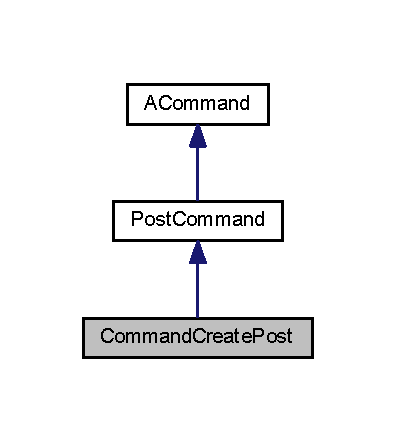
\includegraphics[width=190pt]{class_command_create_post__inherit__graph}
\end{center}
\end{figure}


Collaboration diagram for Command\-Create\-Post\-:\nopagebreak
\begin{figure}[H]
\begin{center}
\leavevmode
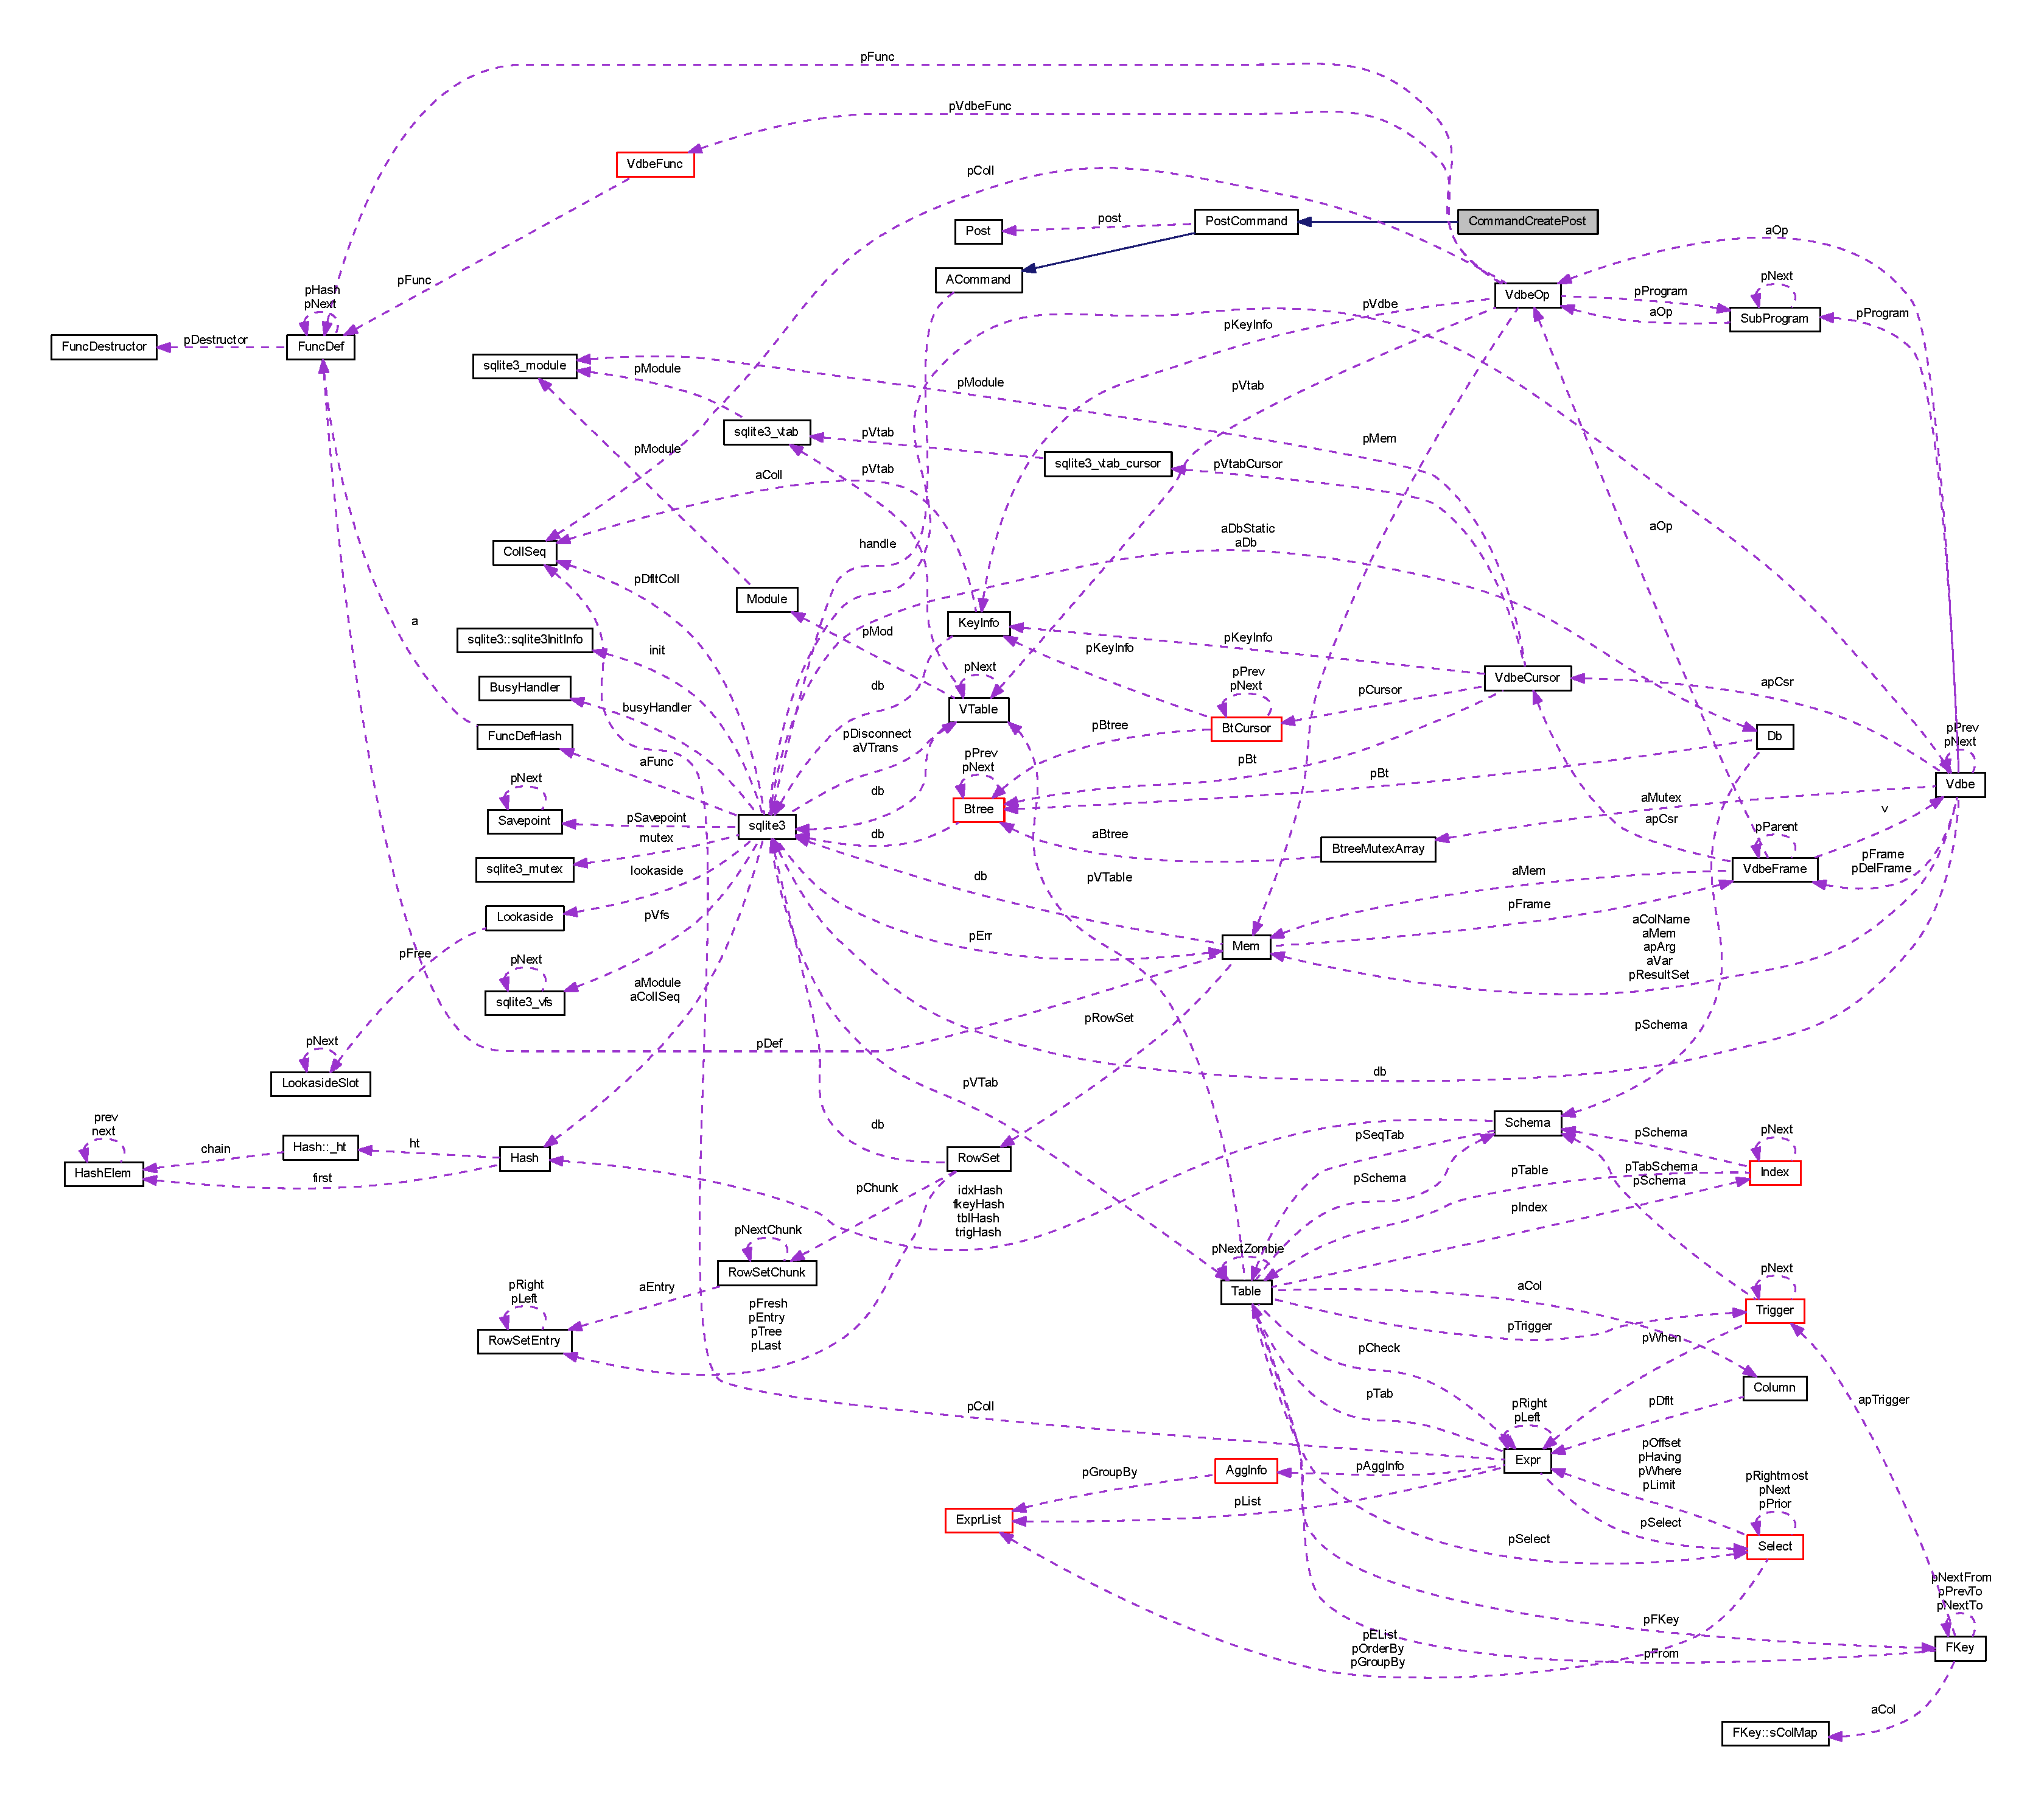
\includegraphics[width=350pt]{class_command_create_post__coll__graph}
\end{center}
\end{figure}
\subsection*{Public Member Functions}
\begin{DoxyCompactItemize}
\item 
void \hyperlink{class_command_create_post_ad13e9a228becc94f51d035875500eb69}{execute} ()
\begin{DoxyCompactList}\small\item\em Método responsável por iniciar a execução da classe. \end{DoxyCompactList}\end{DoxyCompactItemize}
\subsection*{Additional Inherited Members}


\subsection{Detailed Description}
Classe que irá procurar se já existe um id,igual ao do objeto, no bd, se esse não existir irá adicionar o obj. 

\subsection{Member Function Documentation}
\hypertarget{class_command_create_post_ad13e9a228becc94f51d035875500eb69}{\index{Command\-Create\-Post@{Command\-Create\-Post}!execute@{execute}}
\index{execute@{execute}!CommandCreatePost@{Command\-Create\-Post}}
\subsubsection[{execute}]{\setlength{\rightskip}{0pt plus 5cm}void Command\-Create\-Post\-::execute (
\begin{DoxyParamCaption}
{}
\end{DoxyParamCaption}
)\hspace{0.3cm}{\ttfamily [virtual]}}}\label{class_command_create_post_ad13e9a228becc94f51d035875500eb69}


Método responsável por iniciar a execução da classe. 

I\-D já existe 

Implements \hyperlink{class_a_command_a94c6a1d25eb0427389e15450019ebad8}{A\-Command}.



Here is the call graph for this function\-:\nopagebreak
\begin{figure}[H]
\begin{center}
\leavevmode
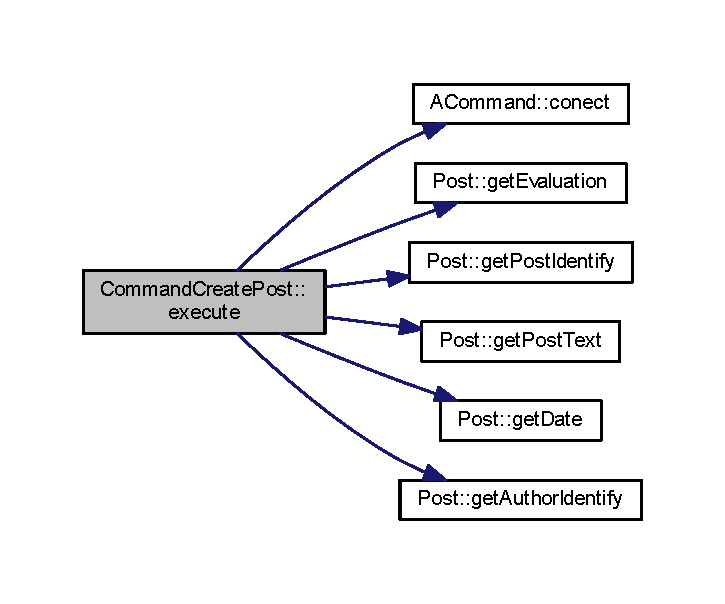
\includegraphics[width=336pt]{class_command_create_post_ad13e9a228becc94f51d035875500eb69_cgraph}
\end{center}
\end{figure}




The documentation for this class was generated from the following files\-:\begin{DoxyCompactItemize}
\item 
Comand.\-h\item 
Comand.\-cpp\end{DoxyCompactItemize}

\hypertarget{class_command_create_user}{\section{Command\-Create\-User Class Reference}
\label{class_command_create_user}\index{Command\-Create\-User@{Command\-Create\-User}}
}


Classe que irá procurar se já existe um id ou um nome ,igual ao do objeto, no bd, se esse não existir irá adicionar o obj.  




{\ttfamily \#include $<$Comand.\-h$>$}



Inheritance diagram for Command\-Create\-User\-:\nopagebreak
\begin{figure}[H]
\begin{center}
\leavevmode
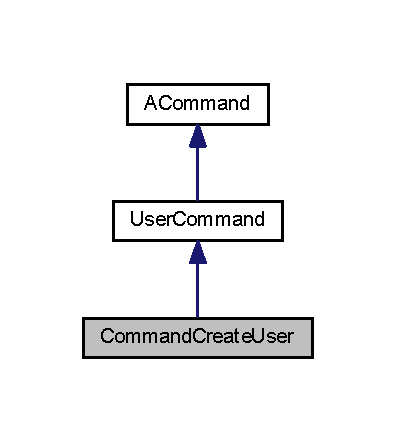
\includegraphics[width=190pt]{class_command_create_user__inherit__graph}
\end{center}
\end{figure}


Collaboration diagram for Command\-Create\-User\-:\nopagebreak
\begin{figure}[H]
\begin{center}
\leavevmode
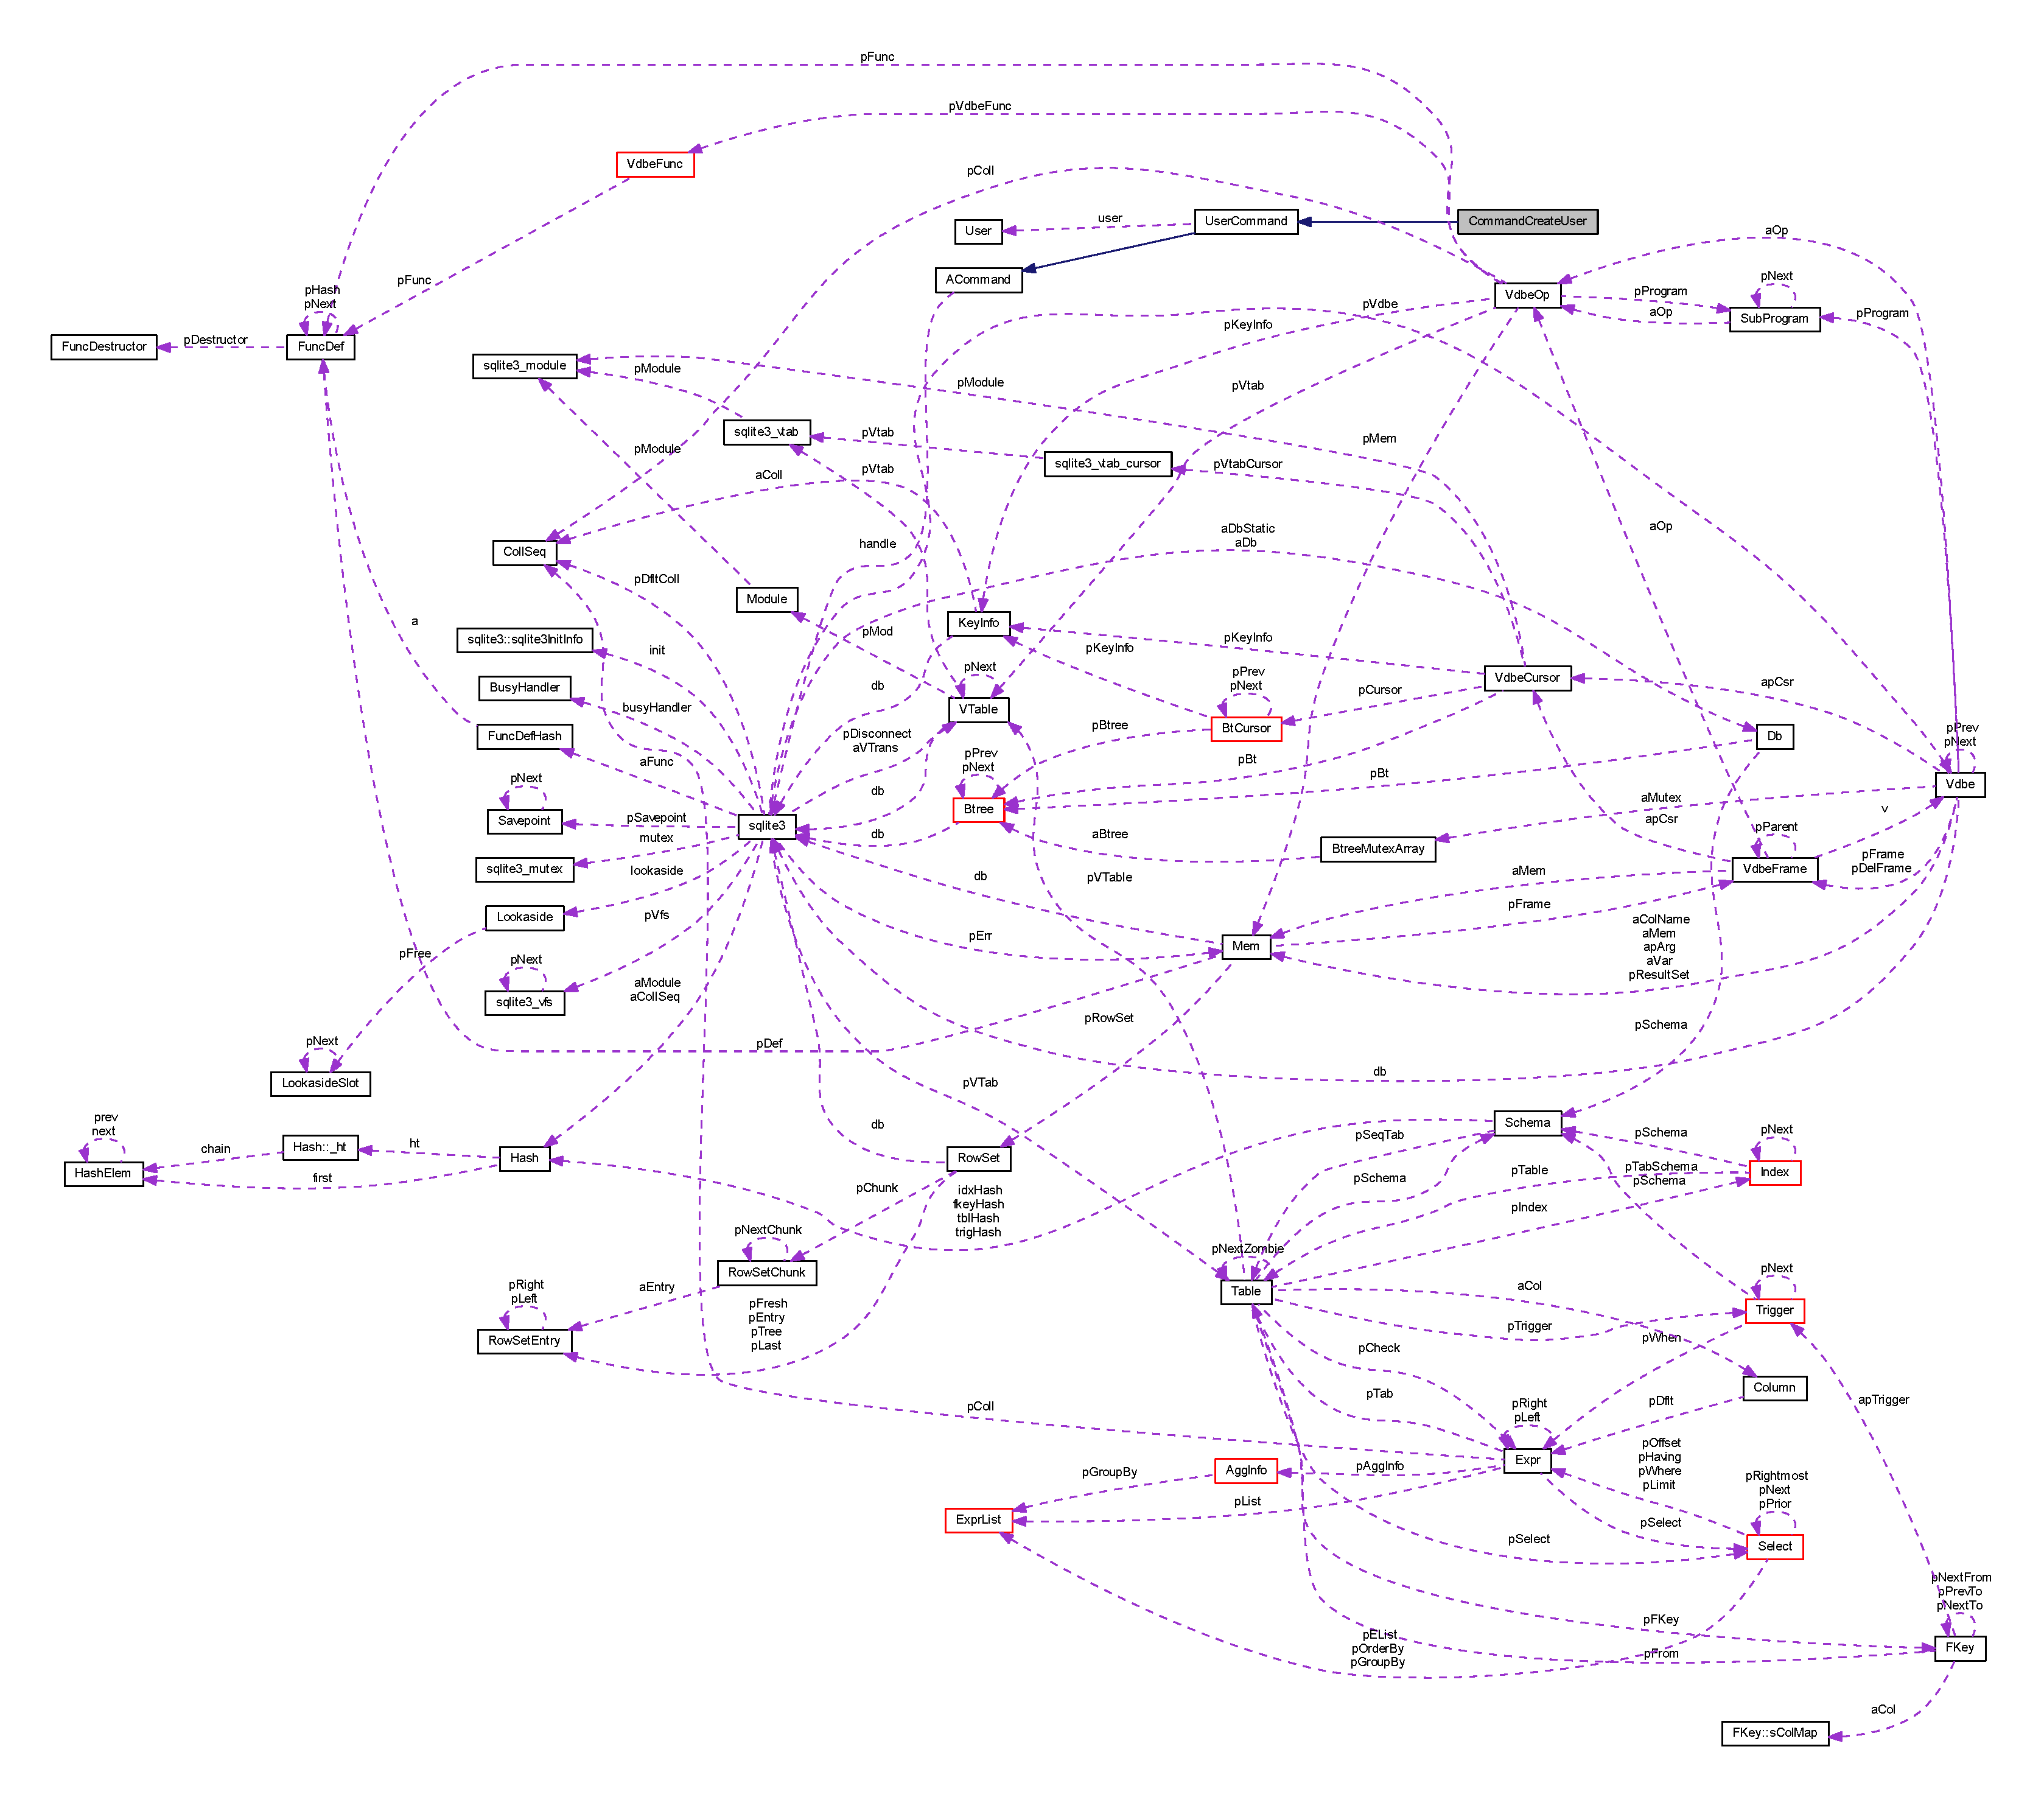
\includegraphics[width=350pt]{class_command_create_user__coll__graph}
\end{center}
\end{figure}
\subsection*{Public Member Functions}
\begin{DoxyCompactItemize}
\item 
void \hyperlink{class_command_create_user_a63ef962dcd3713947dc1fdbcf6a4039e}{execute} ()
\begin{DoxyCompactList}\small\item\em Método responsável por iniciar a execução da classe. \end{DoxyCompactList}\end{DoxyCompactItemize}
\subsection*{Additional Inherited Members}


\subsection{Detailed Description}
Classe que irá procurar se já existe um id ou um nome ,igual ao do objeto, no bd, se esse não existir irá adicionar o obj. 

\subsection{Member Function Documentation}
\hypertarget{class_command_create_user_a63ef962dcd3713947dc1fdbcf6a4039e}{\index{Command\-Create\-User@{Command\-Create\-User}!execute@{execute}}
\index{execute@{execute}!CommandCreateUser@{Command\-Create\-User}}
\subsubsection[{execute}]{\setlength{\rightskip}{0pt plus 5cm}void Command\-Create\-User\-::execute (
\begin{DoxyParamCaption}
{}
\end{DoxyParamCaption}
)\hspace{0.3cm}{\ttfamily [virtual]}}}\label{class_command_create_user_a63ef962dcd3713947dc1fdbcf6a4039e}


Método responsável por iniciar a execução da classe. 

I\-D ou N\-O\-M\-E já existe 

Implements \hyperlink{class_a_command_a94c6a1d25eb0427389e15450019ebad8}{A\-Command}.



Here is the call graph for this function\-:\nopagebreak
\begin{figure}[H]
\begin{center}
\leavevmode
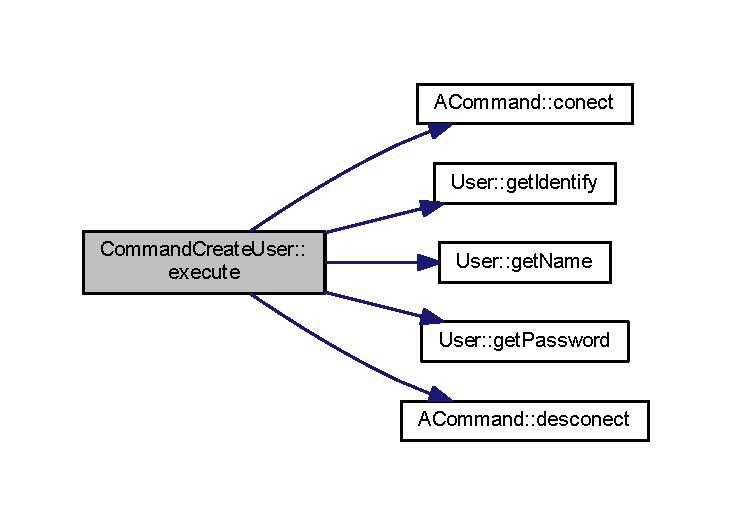
\includegraphics[width=350pt]{class_command_create_user_a63ef962dcd3713947dc1fdbcf6a4039e_cgraph}
\end{center}
\end{figure}




The documentation for this class was generated from the following files\-:\begin{DoxyCompactItemize}
\item 
Comand.\-h\item 
Comand.\-cpp\end{DoxyCompactItemize}

\hypertarget{class_command_delete_coment}{\section{Command\-Delete\-Coment Class Reference}
\label{class_command_delete_coment}\index{Command\-Delete\-Coment@{Command\-Delete\-Coment}}
}


Classe que irá deletar um comentário no banco de dados, caso esse exista.  




{\ttfamily \#include $<$Comand.\-h$>$}



Inheritance diagram for Command\-Delete\-Coment\-:\nopagebreak
\begin{figure}[H]
\begin{center}
\leavevmode
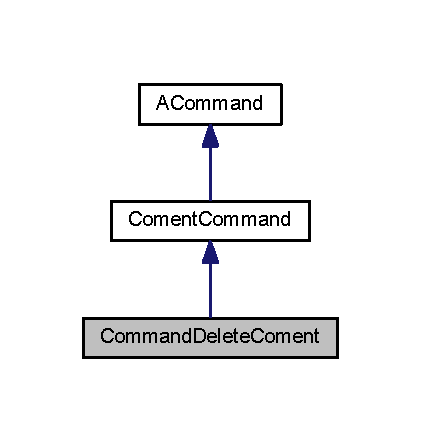
\includegraphics[width=202pt]{class_command_delete_coment__inherit__graph}
\end{center}
\end{figure}


Collaboration diagram for Command\-Delete\-Coment\-:\nopagebreak
\begin{figure}[H]
\begin{center}
\leavevmode
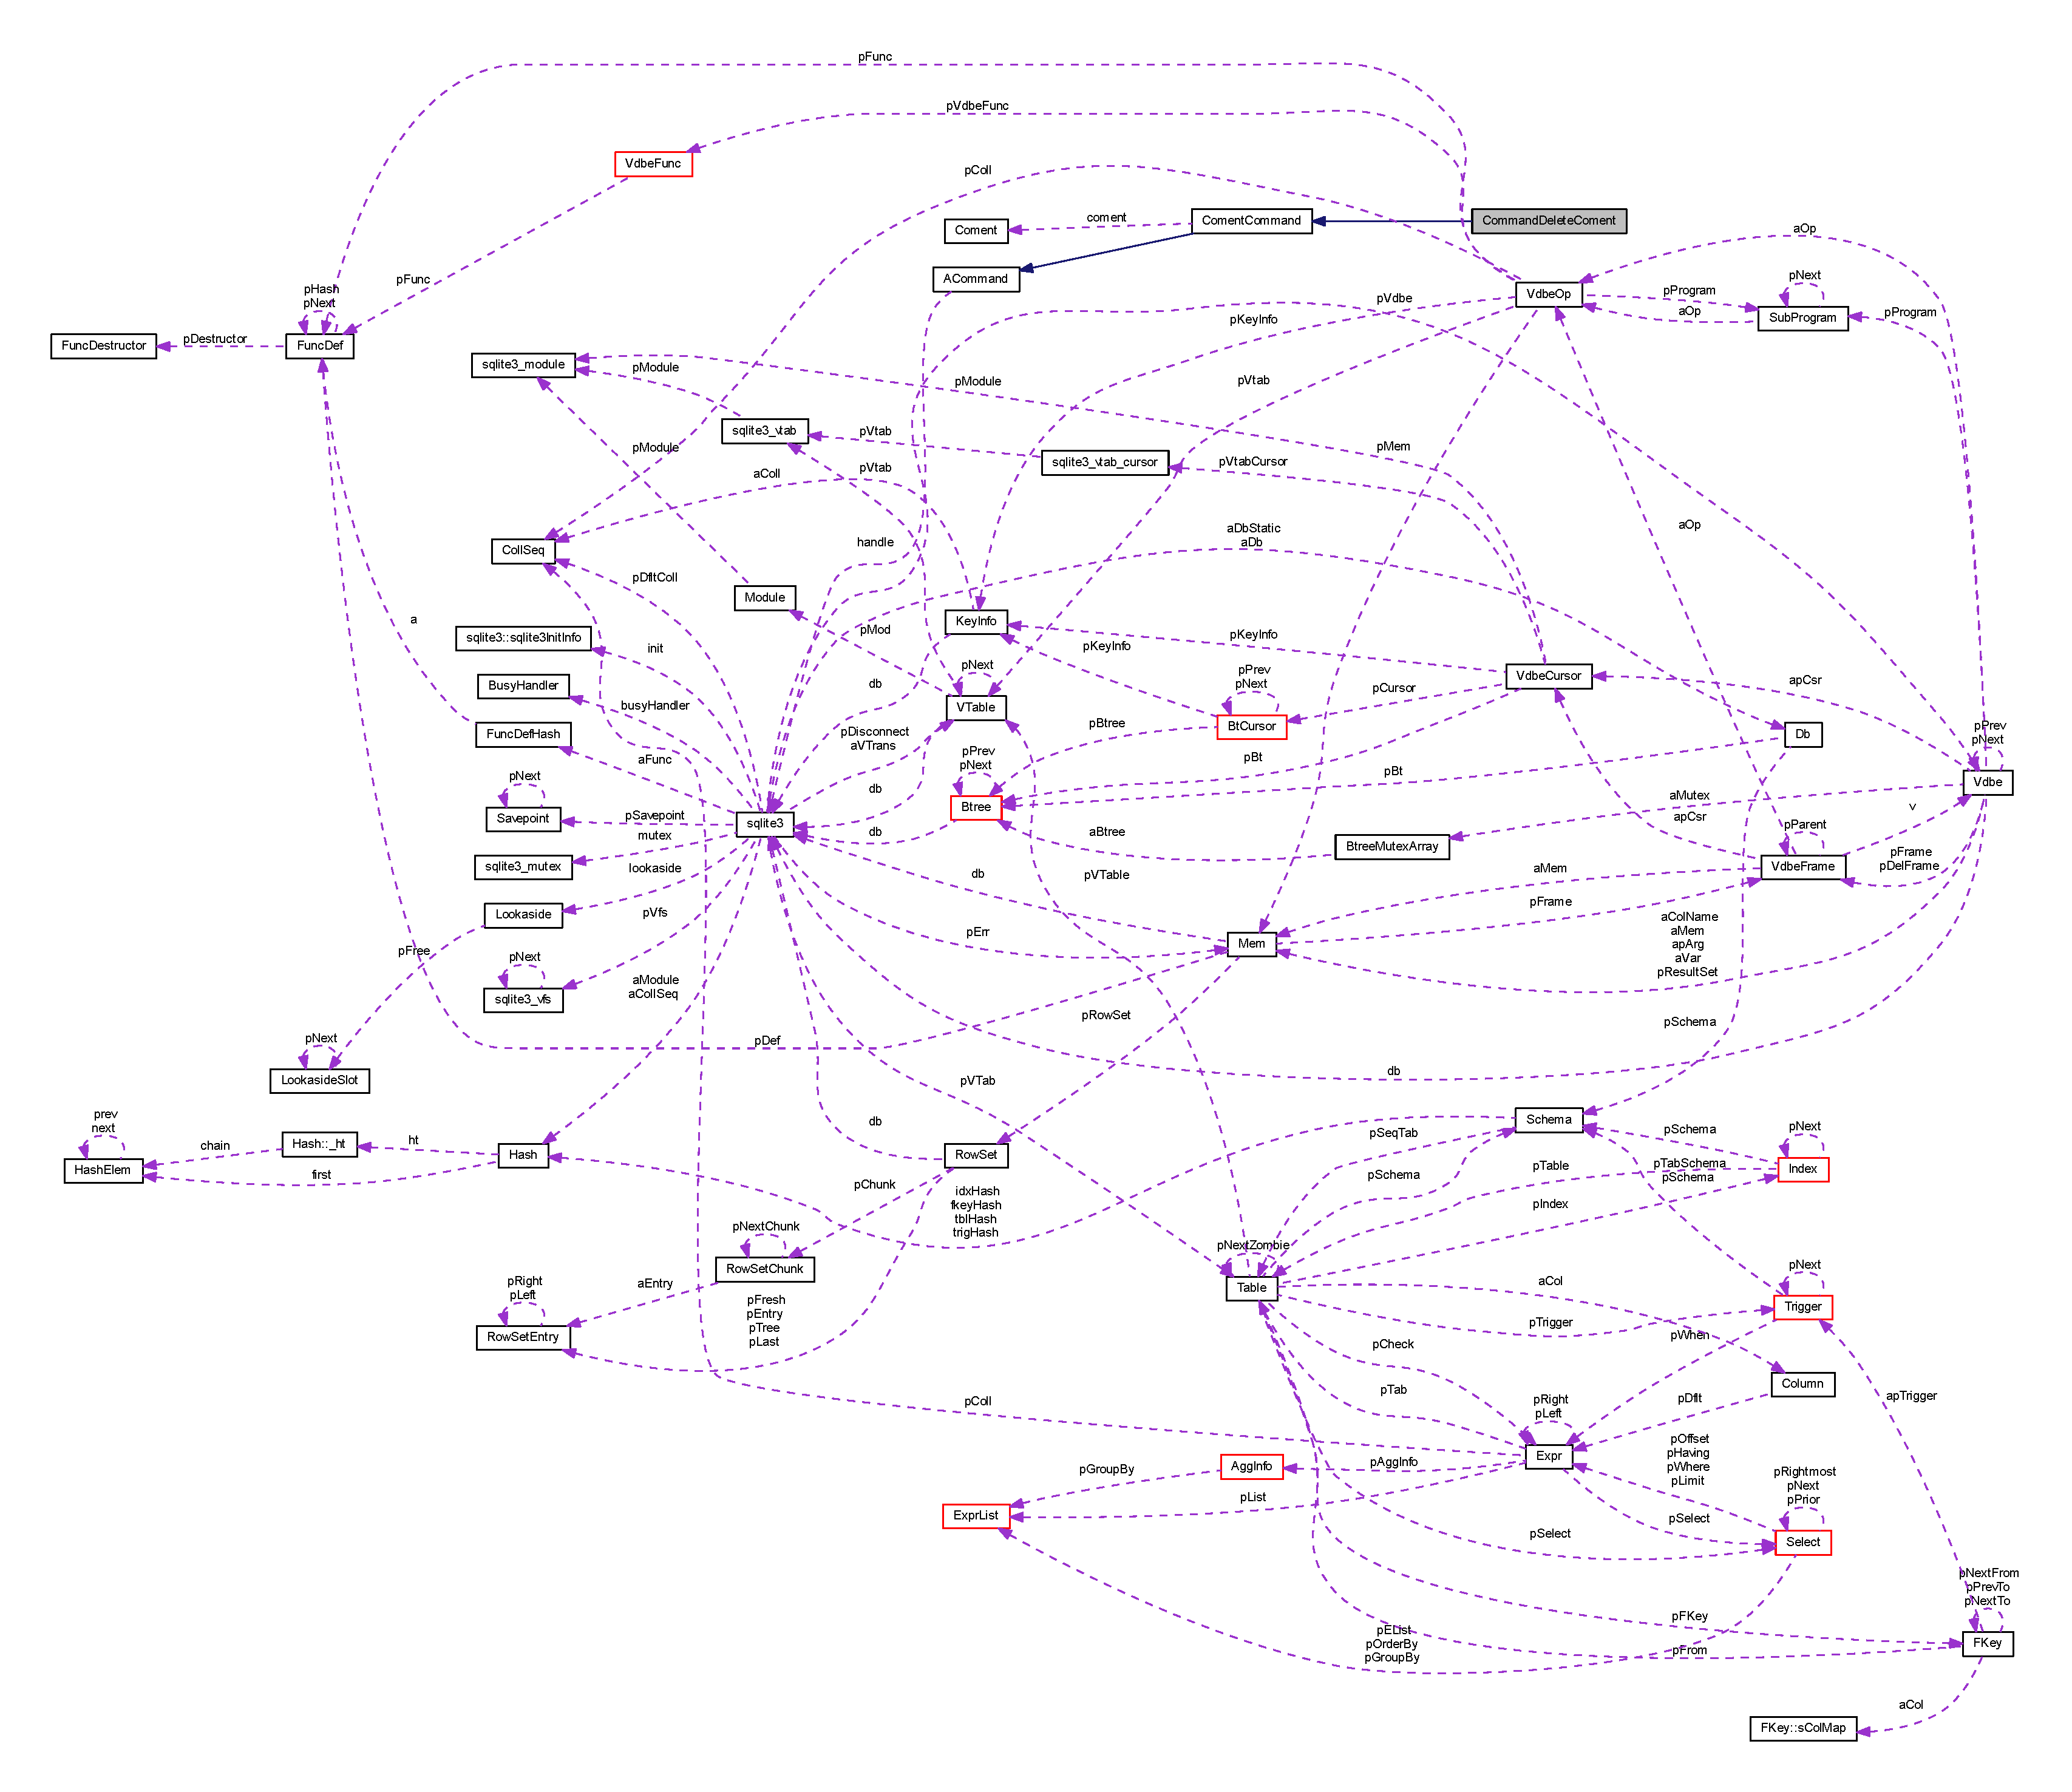
\includegraphics[width=350pt]{class_command_delete_coment__coll__graph}
\end{center}
\end{figure}
\subsection*{Public Member Functions}
\begin{DoxyCompactItemize}
\item 
\hypertarget{class_command_delete_coment_ae614055e5d5b28ef6921edbab3b99a7c}{void \hyperlink{class_command_delete_coment_ae614055e5d5b28ef6921edbab3b99a7c}{execute} ()}\label{class_command_delete_coment_ae614055e5d5b28ef6921edbab3b99a7c}

\begin{DoxyCompactList}\small\item\em Método responsável por iniciar a execução da classe. \end{DoxyCompactList}\end{DoxyCompactItemize}
\subsection*{Additional Inherited Members}


\subsection{Detailed Description}
Classe que irá deletar um comentário no banco de dados, caso esse exista. 

The documentation for this class was generated from the following files\-:\begin{DoxyCompactItemize}
\item 
C\-:/\-Users/\-Vitor/\-Desktop/\-Work\-Space/\-P\-R\-O\-J\-E\-T\-O\-\_\-\-F\-I\-N\-A\-L\-\_\-\-P\-O\-O/\-P\-R\-O\-J\-E\-T\-O\-\_\-\-D\-E\-V/\-P\-R\-O\-J\-E\-T\-O/\-Projeto\-\_\-codeblocks/Comand.\-h\item 
C\-:/\-Users/\-Vitor/\-Desktop/\-Work\-Space/\-P\-R\-O\-J\-E\-T\-O\-\_\-\-F\-I\-N\-A\-L\-\_\-\-P\-O\-O/\-P\-R\-O\-J\-E\-T\-O\-\_\-\-D\-E\-V/\-P\-R\-O\-J\-E\-T\-O/\-Projeto\-\_\-codeblocks/Comand.\-cpp\end{DoxyCompactItemize}

\hypertarget{class_command_delete_post}{\section{Command\-Delete\-Post Class Reference}
\label{class_command_delete_post}\index{Command\-Delete\-Post@{Command\-Delete\-Post}}
}


Classe que irá deletar um post no banco de dados, caso esse exista.  




{\ttfamily \#include $<$Comand.\-h$>$}



Inheritance diagram for Command\-Delete\-Post\-:\nopagebreak
\begin{figure}[H]
\begin{center}
\leavevmode
\includegraphics[width=188pt]{class_command_delete_post__inherit__graph}
\end{center}
\end{figure}


Collaboration diagram for Command\-Delete\-Post\-:\nopagebreak
\begin{figure}[H]
\begin{center}
\leavevmode
\includegraphics[width=350pt]{class_command_delete_post__coll__graph}
\end{center}
\end{figure}
\subsection*{Public Member Functions}
\begin{DoxyCompactItemize}
\item 
\hypertarget{class_command_delete_post_af93e629833de0fa3415294802258d243}{void \hyperlink{class_command_delete_post_af93e629833de0fa3415294802258d243}{execute} ()}\label{class_command_delete_post_af93e629833de0fa3415294802258d243}

\begin{DoxyCompactList}\small\item\em Método responsável por iniciar a execução da classe. \end{DoxyCompactList}\end{DoxyCompactItemize}
\subsection*{Additional Inherited Members}


\subsection{Detailed Description}
Classe que irá deletar um post no banco de dados, caso esse exista. 

The documentation for this class was generated from the following files\-:\begin{DoxyCompactItemize}
\item 
Comand.\-h\item 
Comand.\-cpp\end{DoxyCompactItemize}

\hypertarget{class_command_delete_user}{\section{Command\-Delete\-User Class Reference}
\label{class_command_delete_user}\index{Command\-Delete\-User@{Command\-Delete\-User}}
}


Classe que irá deletar um usuário no banco de dados, caso esse exista.  




{\ttfamily \#include $<$Comand.\-h$>$}



Inheritance diagram for Command\-Delete\-User\-:\nopagebreak
\begin{figure}[H]
\begin{center}
\leavevmode
\includegraphics[width=188pt]{class_command_delete_user__inherit__graph}
\end{center}
\end{figure}


Collaboration diagram for Command\-Delete\-User\-:\nopagebreak
\begin{figure}[H]
\begin{center}
\leavevmode
\includegraphics[width=350pt]{class_command_delete_user__coll__graph}
\end{center}
\end{figure}
\subsection*{Public Member Functions}
\begin{DoxyCompactItemize}
\item 
void \hyperlink{class_command_delete_user_aa569e0aa0dfd5954b2d3d4334b63070d}{execute} ()
\begin{DoxyCompactList}\small\item\em Método responsável por iniciar a execução da classe. \end{DoxyCompactList}\end{DoxyCompactItemize}
\subsection*{Additional Inherited Members}


\subsection{Detailed Description}
Classe que irá deletar um usuário no banco de dados, caso esse exista. 

\subsection{Member Function Documentation}
\hypertarget{class_command_delete_user_aa569e0aa0dfd5954b2d3d4334b63070d}{\index{Command\-Delete\-User@{Command\-Delete\-User}!execute@{execute}}
\index{execute@{execute}!CommandDeleteUser@{Command\-Delete\-User}}
\subsubsection[{execute}]{\setlength{\rightskip}{0pt plus 5cm}void Command\-Delete\-User\-::execute (
\begin{DoxyParamCaption}
{}
\end{DoxyParamCaption}
)\hspace{0.3cm}{\ttfamily [virtual]}}}\label{class_command_delete_user_aa569e0aa0dfd5954b2d3d4334b63070d}


Método responsável por iniciar a execução da classe. 

N\-O\-M\-E já existe 

Implements \hyperlink{class_a_command_a94c6a1d25eb0427389e15450019ebad8}{A\-Command}.



Here is the call graph for this function\-:\nopagebreak
\begin{figure}[H]
\begin{center}
\leavevmode
\includegraphics[width=336pt]{class_command_delete_user_aa569e0aa0dfd5954b2d3d4334b63070d_cgraph}
\end{center}
\end{figure}




The documentation for this class was generated from the following files\-:\begin{DoxyCompactItemize}
\item 
C\-:/\-Users/\-Vitor/\-Desktop/\-Work\-Space/\-P\-R\-O\-J\-E\-T\-O\-\_\-\-F\-I\-N\-A\-L\-\_\-\-P\-O\-O/\-P\-R\-O\-J\-E\-T\-O\-\_\-\-D\-E\-V/\-P\-R\-O\-J\-E\-T\-O/\-Projeto\-\_\-codeblocks/Comand.\-h\item 
C\-:/\-Users/\-Vitor/\-Desktop/\-Work\-Space/\-P\-R\-O\-J\-E\-T\-O\-\_\-\-F\-I\-N\-A\-L\-\_\-\-P\-O\-O/\-P\-R\-O\-J\-E\-T\-O\-\_\-\-D\-E\-V/\-P\-R\-O\-J\-E\-T\-O/\-Projeto\-\_\-codeblocks/Comand.\-cpp\end{DoxyCompactItemize}

\hypertarget{class_command_find_all_post}{\section{Command\-Find\-All\-Post Class Reference}
\label{class_command_find_all_post}\index{Command\-Find\-All\-Post@{Command\-Find\-All\-Post}}
}


Classe que irá listar todos os posts.  




{\ttfamily \#include $<$Comand.\-h$>$}



Inheritance diagram for Command\-Find\-All\-Post\-:\nopagebreak
\begin{figure}[H]
\begin{center}
\leavevmode
\includegraphics[width=190pt]{class_command_find_all_post__inherit__graph}
\end{center}
\end{figure}


Collaboration diagram for Command\-Find\-All\-Post\-:\nopagebreak
\begin{figure}[H]
\begin{center}
\leavevmode
\includegraphics[width=350pt]{class_command_find_all_post__coll__graph}
\end{center}
\end{figure}
\subsection*{Public Member Functions}
\begin{DoxyCompactItemize}
\item 
\hypertarget{class_command_find_all_post_a701c5ce055da556f02e95e33ef2a7334}{void \hyperlink{class_command_find_all_post_a701c5ce055da556f02e95e33ef2a7334}{execute} ()}\label{class_command_find_all_post_a701c5ce055da556f02e95e33ef2a7334}

\begin{DoxyCompactList}\small\item\em Método responsável por iniciar a execução da classe. \end{DoxyCompactList}\end{DoxyCompactItemize}
\subsection*{Additional Inherited Members}


\subsection{Detailed Description}
Classe que irá listar todos os posts. 

The documentation for this class was generated from the following files\-:\begin{DoxyCompactItemize}
\item 
Comand.\-h\item 
Comand.\-cpp\end{DoxyCompactItemize}

\hypertarget{class_command_find_coment}{\section{Command\-Find\-Coment Class Reference}
\label{class_command_find_coment}\index{Command\-Find\-Coment@{Command\-Find\-Coment}}
}


Classe que irá procurar um cometário pelo id, se encontrar o coloca em um objeto Coment.  




{\ttfamily \#include $<$Comand.\-h$>$}



Inheritance diagram for Command\-Find\-Coment\-:\nopagebreak
\begin{figure}[H]
\begin{center}
\leavevmode
\includegraphics[width=192pt]{class_command_find_coment__inherit__graph}
\end{center}
\end{figure}


Collaboration diagram for Command\-Find\-Coment\-:\nopagebreak
\begin{figure}[H]
\begin{center}
\leavevmode
\includegraphics[width=350pt]{class_command_find_coment__coll__graph}
\end{center}
\end{figure}
\subsection*{Public Member Functions}
\begin{DoxyCompactItemize}
\item 
\hypertarget{class_command_find_coment_a5e0b7e24dbe78155bfef3a3e12f329de}{void \hyperlink{class_command_find_coment_a5e0b7e24dbe78155bfef3a3e12f329de}{execute} ()}\label{class_command_find_coment_a5e0b7e24dbe78155bfef3a3e12f329de}

\begin{DoxyCompactList}\small\item\em Método responsável por iniciar a execução da classe. \end{DoxyCompactList}\end{DoxyCompactItemize}
\subsection*{Additional Inherited Members}


\subsection{Detailed Description}
Classe que irá procurar um cometário pelo id, se encontrar o coloca em um objeto Coment. 

The documentation for this class was generated from the following files\-:\begin{DoxyCompactItemize}
\item 
Comand.\-h\item 
Comand.\-cpp\end{DoxyCompactItemize}

\hypertarget{class_command_find_post}{\section{Command\-Find\-Post Class Reference}
\label{class_command_find_post}\index{Command\-Find\-Post@{Command\-Find\-Post}}
}


Classe que irá procurar um post pelo id, se encontrar o coloca em um objeto \hyperlink{class_post}{Post}.  




{\ttfamily \#include $<$Comand.\-h$>$}



Inheritance diagram for Command\-Find\-Post\-:\nopagebreak
\begin{figure}[H]
\begin{center}
\leavevmode
\includegraphics[width=180pt]{class_command_find_post__inherit__graph}
\end{center}
\end{figure}


Collaboration diagram for Command\-Find\-Post\-:\nopagebreak
\begin{figure}[H]
\begin{center}
\leavevmode
\includegraphics[width=350pt]{class_command_find_post__coll__graph}
\end{center}
\end{figure}
\subsection*{Public Member Functions}
\begin{DoxyCompactItemize}
\item 
\hypertarget{class_command_find_post_a271fd0e0c327fe009caa71a4df92a454}{void \hyperlink{class_command_find_post_a271fd0e0c327fe009caa71a4df92a454}{execute} ()}\label{class_command_find_post_a271fd0e0c327fe009caa71a4df92a454}

\begin{DoxyCompactList}\small\item\em Método responsável por iniciar a execução da classe. \end{DoxyCompactList}\end{DoxyCompactItemize}
\subsection*{Additional Inherited Members}


\subsection{Detailed Description}
Classe que irá procurar um post pelo id, se encontrar o coloca em um objeto \hyperlink{class_post}{Post}. 

The documentation for this class was generated from the following files\-:\begin{DoxyCompactItemize}
\item 
C\-:/\-Users/\-Vitor/\-Desktop/\-Work\-Space/\-P\-R\-O\-J\-E\-T\-O\-\_\-\-F\-I\-N\-A\-L\-\_\-\-P\-O\-O/\-P\-R\-O\-J\-E\-T\-O\-\_\-\-D\-E\-V/\-P\-R\-O\-J\-E\-T\-O/\-Projeto\-\_\-codeblocks/Comand.\-h\item 
C\-:/\-Users/\-Vitor/\-Desktop/\-Work\-Space/\-P\-R\-O\-J\-E\-T\-O\-\_\-\-F\-I\-N\-A\-L\-\_\-\-P\-O\-O/\-P\-R\-O\-J\-E\-T\-O\-\_\-\-D\-E\-V/\-P\-R\-O\-J\-E\-T\-O/\-Projeto\-\_\-codeblocks/Comand.\-cpp\end{DoxyCompactItemize}

\hypertarget{class_command_find_post_coments}{\section{Command\-Find\-Post\-Coments Class Reference}
\label{class_command_find_post_coments}\index{Command\-Find\-Post\-Coments@{Command\-Find\-Post\-Coments}}
}


Classe que irá procurar os comentários de um post, se encontrar os coloca em um lista de objetos \hyperlink{class_coment}{Coment}.  




{\ttfamily \#include $<$Comand.\-h$>$}



Inheritance diagram for Command\-Find\-Post\-Coments\-:\nopagebreak
\begin{figure}[H]
\begin{center}
\leavevmode
\includegraphics[width=218pt]{class_command_find_post_coments__inherit__graph}
\end{center}
\end{figure}


Collaboration diagram for Command\-Find\-Post\-Coments\-:\nopagebreak
\begin{figure}[H]
\begin{center}
\leavevmode
\includegraphics[width=350pt]{class_command_find_post_coments__coll__graph}
\end{center}
\end{figure}
\subsection*{Public Member Functions}
\begin{DoxyCompactItemize}
\item 
\hypertarget{class_command_find_post_coments_a9e9fdb81a5355d61e93e803adbcf5257}{void \hyperlink{class_command_find_post_coments_a9e9fdb81a5355d61e93e803adbcf5257}{execute} ()}\label{class_command_find_post_coments_a9e9fdb81a5355d61e93e803adbcf5257}

\begin{DoxyCompactList}\small\item\em Método responsável por iniciar a execução da classe. \end{DoxyCompactList}\end{DoxyCompactItemize}
\subsection*{Additional Inherited Members}


\subsection{Detailed Description}
Classe que irá procurar os comentários de um post, se encontrar os coloca em um lista de objetos \hyperlink{class_coment}{Coment}. 

The documentation for this class was generated from the following files\-:\begin{DoxyCompactItemize}
\item 
C\-:/\-Users/\-Vitor/\-Desktop/\-Work\-Space/\-P\-R\-O\-J\-E\-T\-O\-\_\-\-F\-I\-N\-A\-L\-\_\-\-P\-O\-O/\-P\-R\-O\-J\-E\-T\-O\-\_\-\-D\-E\-V/\-P\-R\-O\-J\-E\-T\-O/\-Projeto\-\_\-codeblocks/Comand.\-h\item 
C\-:/\-Users/\-Vitor/\-Desktop/\-Work\-Space/\-P\-R\-O\-J\-E\-T\-O\-\_\-\-F\-I\-N\-A\-L\-\_\-\-P\-O\-O/\-P\-R\-O\-J\-E\-T\-O\-\_\-\-D\-E\-V/\-P\-R\-O\-J\-E\-T\-O/\-Projeto\-\_\-codeblocks/Comand.\-cpp\end{DoxyCompactItemize}

\hypertarget{class_command_find_user}{\section{Command\-Find\-User Class Reference}
\label{class_command_find_user}\index{Command\-Find\-User@{Command\-Find\-User}}
}


Classe que irá procurar um usuário pelo id e o colocara no objeto.  




{\ttfamily \#include $<$Comand.\-h$>$}



Inheritance diagram for Command\-Find\-User\-:\nopagebreak
\begin{figure}[H]
\begin{center}
\leavevmode
\includegraphics[width=180pt]{class_command_find_user__inherit__graph}
\end{center}
\end{figure}


Collaboration diagram for Command\-Find\-User\-:\nopagebreak
\begin{figure}[H]
\begin{center}
\leavevmode
\includegraphics[width=350pt]{class_command_find_user__coll__graph}
\end{center}
\end{figure}
\subsection*{Public Member Functions}
\begin{DoxyCompactItemize}
\item 
\hypertarget{class_command_find_user_a5ec31dbc1a789b3df354bf05f8cca046}{void \hyperlink{class_command_find_user_a5ec31dbc1a789b3df354bf05f8cca046}{execute} ()}\label{class_command_find_user_a5ec31dbc1a789b3df354bf05f8cca046}

\begin{DoxyCompactList}\small\item\em Método responsável por iniciar a execução da classe. \end{DoxyCompactList}\end{DoxyCompactItemize}
\subsection*{Additional Inherited Members}


\subsection{Detailed Description}
Classe que irá procurar um usuário pelo id e o colocara no objeto. 

The documentation for this class was generated from the following files\-:\begin{DoxyCompactItemize}
\item 
Comand.\-h\item 
Comand.\-cpp\end{DoxyCompactItemize}

\hypertarget{class_command_find_user_post}{\section{Command\-Find\-User\-Post Class Reference}
\label{class_command_find_user_post}\index{Command\-Find\-User\-Post@{Command\-Find\-User\-Post}}
}


Classe que retorna os posts de um usário que estão no banco de dados.  




{\ttfamily \#include $<$Comand.\-h$>$}



Inheritance diagram for Command\-Find\-User\-Post\-:\nopagebreak
\begin{figure}[H]
\begin{center}
\leavevmode
\includegraphics[width=200pt]{class_command_find_user_post__inherit__graph}
\end{center}
\end{figure}


Collaboration diagram for Command\-Find\-User\-Post\-:\nopagebreak
\begin{figure}[H]
\begin{center}
\leavevmode
\includegraphics[width=350pt]{class_command_find_user_post__coll__graph}
\end{center}
\end{figure}
\subsection*{Public Member Functions}
\begin{DoxyCompactItemize}
\item 
\hypertarget{class_command_find_user_post_a2a28fed7b287b88274b60d8e4524f6de}{void \hyperlink{class_command_find_user_post_a2a28fed7b287b88274b60d8e4524f6de}{execute} ()}\label{class_command_find_user_post_a2a28fed7b287b88274b60d8e4524f6de}

\begin{DoxyCompactList}\small\item\em Método responsável por iniciar a execução da classe. \end{DoxyCompactList}\end{DoxyCompactItemize}
\subsection*{Additional Inherited Members}


\subsection{Detailed Description}
Classe que retorna os posts de um usário que estão no banco de dados. 

The documentation for this class was generated from the following files\-:\begin{DoxyCompactItemize}
\item 
Comand.\-h\item 
Comand.\-cpp\end{DoxyCompactItemize}

\hypertarget{class_command_find_users}{\section{Command\-Find\-Users Class Reference}
\label{class_command_find_users}\index{Command\-Find\-Users@{Command\-Find\-Users}}
}


Classe que irá listar todos os usuários.  




{\ttfamily \#include $<$Comand.\-h$>$}



Inheritance diagram for Command\-Find\-Users\-:\nopagebreak
\begin{figure}[H]
\begin{center}
\leavevmode
\includegraphics[width=184pt]{class_command_find_users__inherit__graph}
\end{center}
\end{figure}


Collaboration diagram for Command\-Find\-Users\-:\nopagebreak
\begin{figure}[H]
\begin{center}
\leavevmode
\includegraphics[width=350pt]{class_command_find_users__coll__graph}
\end{center}
\end{figure}
\subsection*{Public Member Functions}
\begin{DoxyCompactItemize}
\item 
\hypertarget{class_command_find_users_ab33e1107a64b988eaa31bf1e7611c990}{void \hyperlink{class_command_find_users_ab33e1107a64b988eaa31bf1e7611c990}{execute} ()}\label{class_command_find_users_ab33e1107a64b988eaa31bf1e7611c990}

\begin{DoxyCompactList}\small\item\em Método responsável por iniciar a execução da classe. \end{DoxyCompactList}\end{DoxyCompactItemize}
\subsection*{Additional Inherited Members}


\subsection{Detailed Description}
Classe que irá listar todos os usuários. 

The documentation for this class was generated from the following files\-:\begin{DoxyCompactItemize}
\item 
Comand.\-h\item 
Comand.\-cpp\end{DoxyCompactItemize}

\hypertarget{class_command_update_coment}{\section{Command\-Update\-Coment Class Reference}
\label{class_command_update_coment}\index{Command\-Update\-Coment@{Command\-Update\-Coment}}
}


Classe que irá atualizar um comentário no banco de dados, caso esse exista.  




{\ttfamily \#include $<$Comand.\-h$>$}



Inheritance diagram for Command\-Update\-Coment\-:\nopagebreak
\begin{figure}[H]
\begin{center}
\leavevmode
\includegraphics[width=204pt]{class_command_update_coment__inherit__graph}
\end{center}
\end{figure}


Collaboration diagram for Command\-Update\-Coment\-:\nopagebreak
\begin{figure}[H]
\begin{center}
\leavevmode
\includegraphics[width=350pt]{class_command_update_coment__coll__graph}
\end{center}
\end{figure}
\subsection*{Public Member Functions}
\begin{DoxyCompactItemize}
\item 
void \hyperlink{class_command_update_coment_a77c2f791e6b04b249fc7fbb36b66bf0a}{execute} ()
\begin{DoxyCompactList}\small\item\em Método responsável por iniciar a execução da classe. \end{DoxyCompactList}\end{DoxyCompactItemize}
\subsection*{Additional Inherited Members}


\subsection{Detailed Description}
Classe que irá atualizar um comentário no banco de dados, caso esse exista. 

\subsection{Member Function Documentation}
\hypertarget{class_command_update_coment_a77c2f791e6b04b249fc7fbb36b66bf0a}{\index{Command\-Update\-Coment@{Command\-Update\-Coment}!execute@{execute}}
\index{execute@{execute}!CommandUpdateComent@{Command\-Update\-Coment}}
\subsubsection[{execute}]{\setlength{\rightskip}{0pt plus 5cm}void Command\-Update\-Coment\-::execute (
\begin{DoxyParamCaption}
{}
\end{DoxyParamCaption}
)\hspace{0.3cm}{\ttfamily [virtual]}}}\label{class_command_update_coment_a77c2f791e6b04b249fc7fbb36b66bf0a}


Método responsável por iniciar a execução da classe. 

B\-U\-G 

Implements \hyperlink{class_a_command_a94c6a1d25eb0427389e15450019ebad8}{A\-Command}.



Here is the call graph for this function\-:\nopagebreak
\begin{figure}[H]
\begin{center}
\leavevmode
\includegraphics[width=346pt]{class_command_update_coment_a77c2f791e6b04b249fc7fbb36b66bf0a_cgraph}
\end{center}
\end{figure}




The documentation for this class was generated from the following files\-:\begin{DoxyCompactItemize}
\item 
Comand.\-h\item 
Comand.\-cpp\end{DoxyCompactItemize}

\hypertarget{class_command_update_post}{\section{Command\-Update\-Post Class Reference}
\label{class_command_update_post}\index{Command\-Update\-Post@{Command\-Update\-Post}}
}


Classe que irá atualizar um post no banco de dados, caso esse exista.  




{\ttfamily \#include $<$Comand.\-h$>$}



Inheritance diagram for Command\-Update\-Post\-:\nopagebreak
\begin{figure}[H]
\begin{center}
\leavevmode
\includegraphics[width=192pt]{class_command_update_post__inherit__graph}
\end{center}
\end{figure}


Collaboration diagram for Command\-Update\-Post\-:\nopagebreak
\begin{figure}[H]
\begin{center}
\leavevmode
\includegraphics[width=350pt]{class_command_update_post__coll__graph}
\end{center}
\end{figure}
\subsection*{Public Member Functions}
\begin{DoxyCompactItemize}
\item 
void \hyperlink{class_command_update_post_a478d3f5f2bd985e18d7dc9f4b7dda74a}{execute} ()
\begin{DoxyCompactList}\small\item\em Método responsável por iniciar a execução da classe. \end{DoxyCompactList}\end{DoxyCompactItemize}
\subsection*{Additional Inherited Members}


\subsection{Detailed Description}
Classe que irá atualizar um post no banco de dados, caso esse exista. 

\subsection{Member Function Documentation}
\hypertarget{class_command_update_post_a478d3f5f2bd985e18d7dc9f4b7dda74a}{\index{Command\-Update\-Post@{Command\-Update\-Post}!execute@{execute}}
\index{execute@{execute}!CommandUpdatePost@{Command\-Update\-Post}}
\subsubsection[{execute}]{\setlength{\rightskip}{0pt plus 5cm}void Command\-Update\-Post\-::execute (
\begin{DoxyParamCaption}
{}
\end{DoxyParamCaption}
)\hspace{0.3cm}{\ttfamily [virtual]}}}\label{class_command_update_post_a478d3f5f2bd985e18d7dc9f4b7dda74a}


Método responsável por iniciar a execução da classe. 

Atualizar I\-D q n existe 

Implements \hyperlink{class_a_command_a94c6a1d25eb0427389e15450019ebad8}{A\-Command}.



Here is the call graph for this function\-:\nopagebreak
\begin{figure}[H]
\begin{center}
\leavevmode
\includegraphics[width=338pt]{class_command_update_post_a478d3f5f2bd985e18d7dc9f4b7dda74a_cgraph}
\end{center}
\end{figure}




The documentation for this class was generated from the following files\-:\begin{DoxyCompactItemize}
\item 
Comand.\-h\item 
Comand.\-cpp\end{DoxyCompactItemize}

\hypertarget{class_command_update_user}{\section{Command\-Update\-User Class Reference}
\label{class_command_update_user}\index{Command\-Update\-User@{Command\-Update\-User}}
}


Classe que irá atualizar um usuário no banco de dados, caso esse exista.  




{\ttfamily \#include $<$Comand.\-h$>$}



Inheritance diagram for Command\-Update\-User\-:\nopagebreak
\begin{figure}[H]
\begin{center}
\leavevmode
\includegraphics[width=192pt]{class_command_update_user__inherit__graph}
\end{center}
\end{figure}


Collaboration diagram for Command\-Update\-User\-:\nopagebreak
\begin{figure}[H]
\begin{center}
\leavevmode
\includegraphics[width=350pt]{class_command_update_user__coll__graph}
\end{center}
\end{figure}
\subsection*{Public Member Functions}
\begin{DoxyCompactItemize}
\item 
void \hyperlink{class_command_update_user_a7cec016985bcdd6584a65e69f19d0ed2}{execute} ()
\begin{DoxyCompactList}\small\item\em Método responsável por iniciar a execução da classe. \end{DoxyCompactList}\end{DoxyCompactItemize}
\subsection*{Additional Inherited Members}


\subsection{Detailed Description}
Classe que irá atualizar um usuário no banco de dados, caso esse exista. 

\subsection{Member Function Documentation}
\hypertarget{class_command_update_user_a7cec016985bcdd6584a65e69f19d0ed2}{\index{Command\-Update\-User@{Command\-Update\-User}!execute@{execute}}
\index{execute@{execute}!CommandUpdateUser@{Command\-Update\-User}}
\subsubsection[{execute}]{\setlength{\rightskip}{0pt plus 5cm}void Command\-Update\-User\-::execute (
\begin{DoxyParamCaption}
{}
\end{DoxyParamCaption}
)\hspace{0.3cm}{\ttfamily [virtual]}}}\label{class_command_update_user_a7cec016985bcdd6584a65e69f19d0ed2}


Método responsável por iniciar a execução da classe. 

N\-O\-M\-E já existe 

Implements \hyperlink{class_a_command_a94c6a1d25eb0427389e15450019ebad8}{A\-Command}.



Here is the call graph for this function\-:\nopagebreak
\begin{figure}[H]
\begin{center}
\leavevmode
\includegraphics[width=338pt]{class_command_update_user_a7cec016985bcdd6584a65e69f19d0ed2_cgraph}
\end{center}
\end{figure}




The documentation for this class was generated from the following files\-:\begin{DoxyCompactItemize}
\item 
C\-:/\-Users/\-Vitor/\-Desktop/\-Work\-Space/\-P\-R\-O\-J\-E\-T\-O\-\_\-\-F\-I\-N\-A\-L\-\_\-\-P\-O\-O/\-P\-R\-O\-J\-E\-T\-O\-\_\-\-D\-E\-V/\-P\-R\-O\-J\-E\-T\-O/\-Projeto\-\_\-codeblocks/Comand.\-h\item 
C\-:/\-Users/\-Vitor/\-Desktop/\-Work\-Space/\-P\-R\-O\-J\-E\-T\-O\-\_\-\-F\-I\-N\-A\-L\-\_\-\-P\-O\-O/\-P\-R\-O\-J\-E\-T\-O\-\_\-\-D\-E\-V/\-P\-R\-O\-J\-E\-T\-O/\-Projeto\-\_\-codeblocks/Comand.\-cpp\end{DoxyCompactItemize}

\hypertarget{structcompare_info}{\section{compare\-Info Struct Reference}
\label{structcompare_info}\index{compare\-Info@{compare\-Info}}
}
\subsection*{Public Attributes}
\begin{DoxyCompactItemize}
\item 
\hypertarget{structcompare_info_a1161e850029ef556e6daee856d32b2e2}{u8 {\bfseries match\-All}}\label{structcompare_info_a1161e850029ef556e6daee856d32b2e2}

\item 
\hypertarget{structcompare_info_ab9aabbf6d3df26bad786b532330a2fd7}{u8 {\bfseries match\-One}}\label{structcompare_info_ab9aabbf6d3df26bad786b532330a2fd7}

\item 
\hypertarget{structcompare_info_a5d2ff58a72c9eb7d22f18915c1751655}{u8 {\bfseries match\-Set}}\label{structcompare_info_a5d2ff58a72c9eb7d22f18915c1751655}

\item 
\hypertarget{structcompare_info_a6de76861b066547321f7a255cb7042ab}{u8 {\bfseries no\-Case}}\label{structcompare_info_a6de76861b066547321f7a255cb7042ab}

\end{DoxyCompactItemize}


The documentation for this struct was generated from the following file\-:\begin{DoxyCompactItemize}
\item 
C\-:/\-Users/\-Vitor/\-Desktop/\-Work\-Space/\-P\-R\-O\-J\-E\-T\-O\-\_\-\-F\-I\-N\-A\-L\-\_\-\-P\-O\-O/\-P\-R\-O\-J\-E\-T\-O\-\_\-\-D\-E\-V/\-P\-R\-O\-J\-E\-T\-O/\-Projeto\-\_\-codeblocks/sqlite3.\-c\end{DoxyCompactItemize}

\hypertarget{struct_count_ctx}{\section{Count\-Ctx Struct Reference}
\label{struct_count_ctx}\index{Count\-Ctx@{Count\-Ctx}}
}
\subsection*{Public Attributes}
\begin{DoxyCompactItemize}
\item 
\hypertarget{struct_count_ctx_a141c718918dbfaa183f772bfd7a516f4}{i64 {\bfseries n}}\label{struct_count_ctx_a141c718918dbfaa183f772bfd7a516f4}

\end{DoxyCompactItemize}


The documentation for this struct was generated from the following file\-:\begin{DoxyCompactItemize}
\item 
C\-:/\-Users/\-Vitor/\-Desktop/\-Work\-Space/\-P\-R\-O\-J\-E\-T\-O\-\_\-\-F\-I\-N\-A\-L\-\_\-\-P\-O\-O/\-P\-R\-O\-J\-E\-T\-O\-\_\-\-D\-E\-V/\-P\-R\-O\-J\-E\-T\-O/\-Projeto\-\_\-codeblocks/sqlite3.\-c\end{DoxyCompactItemize}

\hypertarget{class_date}{\section{Date Class Reference}
\label{class_date}\index{Date@{Date}}
}


Essa e a classe responsavel por reprensentar as datas do sistema.  




{\ttfamily \#include $<$Tipos\-Basicos.\-h$>$}



Inheritance diagram for Date\-:\nopagebreak
\begin{figure}[H]
\begin{center}
\leavevmode
\includegraphics[width=142pt]{class_date__inherit__graph}
\end{center}
\end{figure}


Collaboration diagram for Date\-:\nopagebreak
\begin{figure}[H]
\begin{center}
\leavevmode
\includegraphics[width=142pt]{class_date__coll__graph}
\end{center}
\end{figure}
\subsection*{Public Member Functions}
\begin{DoxyCompactItemize}
\item 
\hypertarget{class_date_a4e59ed4ba66eec61c27460c5d09fa1bd}{\hyperlink{class_date_a4e59ed4ba66eec61c27460c5d09fa1bd}{Date} ()  throw (invalid\-\_\-argument)}\label{class_date_a4e59ed4ba66eec61c27460c5d09fa1bd}

\begin{DoxyCompactList}\small\item\em Funcao contrutora data quando essa bao e passa logo essa e posta como null; 
\begin{DoxyExceptions}{Exceptions}
{\em std\-::invalid\-\_\-argument} & quando a classe nao pode ser vazia. \\
\hline
\end{DoxyExceptions}
\end{DoxyCompactList}\item 
\hyperlink{class_date_accd287de5b603241e67e458a72810561}{Date} (const string \&\hyperlink{class_basic_type_af9b2c5cc32647df01083a6802e913dbf}{value})  throw (invalid\-\_\-argument)
\begin{DoxyCompactList}\small\item\em Funcao contrutora do dat quando esta e passada. \end{DoxyCompactList}\end{DoxyCompactItemize}
\subsection*{Additional Inherited Members}


\subsection{Detailed Description}
Essa e a classe responsavel por reprensentar as datas do sistema. 

\subsection{Constructor \& Destructor Documentation}
\hypertarget{class_date_accd287de5b603241e67e458a72810561}{\index{Date@{Date}!Date@{Date}}
\index{Date@{Date}!Date@{Date}}
\subsubsection[{Date}]{\setlength{\rightskip}{0pt plus 5cm}Date\-::\-Date (
\begin{DoxyParamCaption}
\item[{const string \&}]{value}
\end{DoxyParamCaption}
)  throw (invalid\-\_\-argument)}}\label{class_date_accd287de5b603241e67e458a72810561}


Funcao contrutora do dat quando esta e passada. 


\begin{DoxyParams}{Parameters}
{\em value} & \-: a data. \\
\hline
\end{DoxyParams}

\begin{DoxyExceptions}{Exceptions}
{\em std\-::invalid\-\_\-argument} & o argumeto e invalido. \\
\hline
\end{DoxyExceptions}


The documentation for this class was generated from the following files\-:\begin{DoxyCompactItemize}
\item 
C\-:/\-Users/\-Vitor/\-Desktop/\-Work\-Space/\-P\-R\-O\-J\-E\-T\-O\-\_\-\-F\-I\-N\-A\-L\-\_\-\-P\-O\-O/\-P\-R\-O\-J\-E\-T\-O\-\_\-\-D\-E\-V/\-P\-R\-O\-J\-E\-T\-O/\-Projeto\-\_\-codeblocks/\hyperlink{_tipos_basicos_8h}{Tipos\-Basicos.\-h}\item 
C\-:/\-Users/\-Vitor/\-Desktop/\-Work\-Space/\-P\-R\-O\-J\-E\-T\-O\-\_\-\-F\-I\-N\-A\-L\-\_\-\-P\-O\-O/\-P\-R\-O\-J\-E\-T\-O\-\_\-\-D\-E\-V/\-P\-R\-O\-J\-E\-T\-O/\-Projeto\-\_\-codeblocks/Tipos\-Basicos.\-cpp\end{DoxyCompactItemize}

\hypertarget{struct_date_time}{\section{Date\-Time Struct Reference}
\label{struct_date_time}\index{Date\-Time@{Date\-Time}}
}
\subsection*{Public Attributes}
\begin{DoxyCompactItemize}
\item 
\hypertarget{struct_date_time_ae5043d34fa3c3c4dc1121fec886c6f10}{sqlite3\-\_\-int64 {\bfseries i\-J\-D}}\label{struct_date_time_ae5043d34fa3c3c4dc1121fec886c6f10}

\item 
\hypertarget{struct_date_time_ad39449618b2a15128e32766a208753cf}{int {\bfseries Y}}\label{struct_date_time_ad39449618b2a15128e32766a208753cf}

\item 
\hypertarget{struct_date_time_a00e6515603bb5d7c5ce79d3a5a6438a7}{int {\bfseries M}}\label{struct_date_time_a00e6515603bb5d7c5ce79d3a5a6438a7}

\item 
\hypertarget{struct_date_time_a979ec52428a05d2f2ed827345a416fa6}{int {\bfseries D}}\label{struct_date_time_a979ec52428a05d2f2ed827345a416fa6}

\item 
\hypertarget{struct_date_time_a2146547149b65f64e07e1ac6ed8654b6}{int {\bfseries h}}\label{struct_date_time_a2146547149b65f64e07e1ac6ed8654b6}

\item 
\hypertarget{struct_date_time_ac5db527c48331a515bea3b828d1a2254}{int {\bfseries m}}\label{struct_date_time_ac5db527c48331a515bea3b828d1a2254}

\item 
\hypertarget{struct_date_time_a7f5c2e587ee18014982d85eb616f09b8}{int {\bfseries tz}}\label{struct_date_time_a7f5c2e587ee18014982d85eb616f09b8}

\item 
\hypertarget{struct_date_time_a69a803afb69b74206418bda0bc1bcaa2}{double {\bfseries s}}\label{struct_date_time_a69a803afb69b74206418bda0bc1bcaa2}

\item 
\hypertarget{struct_date_time_aaa042bec0879cd922039062433f4b26f}{char {\bfseries valid\-Y\-M\-D}}\label{struct_date_time_aaa042bec0879cd922039062433f4b26f}

\item 
\hypertarget{struct_date_time_aba26b32c6142cf6bfc09db3088b90add}{char {\bfseries valid\-H\-M\-S}}\label{struct_date_time_aba26b32c6142cf6bfc09db3088b90add}

\item 
\hypertarget{struct_date_time_a1962742892150a03dc5d302f43efbb04}{char {\bfseries valid\-J\-D}}\label{struct_date_time_a1962742892150a03dc5d302f43efbb04}

\item 
\hypertarget{struct_date_time_af3dfda2bdbb2183dc1b94f449701b81e}{char {\bfseries valid\-T\-Z}}\label{struct_date_time_af3dfda2bdbb2183dc1b94f449701b81e}

\end{DoxyCompactItemize}


The documentation for this struct was generated from the following file\-:\begin{DoxyCompactItemize}
\item 
C\-:/\-Users/\-Vitor/\-Desktop/\-Work\-Space/\-P\-R\-O\-J\-E\-T\-O\-\_\-\-F\-I\-N\-A\-L\-\_\-\-P\-O\-O/\-P\-R\-O\-J\-E\-T\-O\-\_\-\-D\-E\-V/\-P\-R\-O\-J\-E\-T\-O/\-Projeto\-\_\-codeblocks/sqlite3.\-c\end{DoxyCompactItemize}

\hypertarget{struct_db}{\section{Db Struct Reference}
\label{struct_db}\index{Db@{Db}}
}


Collaboration diagram for Db\-:\nopagebreak
\begin{figure}[H]
\begin{center}
\leavevmode
\includegraphics[width=350pt]{struct_db__coll__graph}
\end{center}
\end{figure}
\subsection*{Public Attributes}
\begin{DoxyCompactItemize}
\item 
\hypertarget{struct_db_a6df2b5d7c8fd68e92cea961d9e3b279b}{char $\ast$ {\bfseries z\-Name}}\label{struct_db_a6df2b5d7c8fd68e92cea961d9e3b279b}

\item 
\hypertarget{struct_db_a0633e5a6abfc39246d07cc6a417a5852}{\hyperlink{struct_btree}{Btree} $\ast$ {\bfseries p\-Bt}}\label{struct_db_a0633e5a6abfc39246d07cc6a417a5852}

\item 
\hypertarget{struct_db_a4c5495ebea317212f0b41aa2795a7bc9}{u8 {\bfseries in\-Trans}}\label{struct_db_a4c5495ebea317212f0b41aa2795a7bc9}

\item 
\hypertarget{struct_db_a04597a5c023d8b328193450b177ff24c}{u8 {\bfseries safety\-\_\-level}}\label{struct_db_a04597a5c023d8b328193450b177ff24c}

\item 
\hypertarget{struct_db_afd8647a83a4a7053231b92814520d6d4}{\hyperlink{struct_schema}{Schema} $\ast$ {\bfseries p\-Schema}}\label{struct_db_afd8647a83a4a7053231b92814520d6d4}

\end{DoxyCompactItemize}


The documentation for this struct was generated from the following file\-:\begin{DoxyCompactItemize}
\item 
C\-:/\-Users/\-Vitor/\-Desktop/\-Work\-Space/\-P\-R\-O\-J\-E\-T\-O\-\_\-\-F\-I\-N\-A\-L\-\_\-\-P\-O\-O/\-P\-R\-O\-J\-E\-T\-O\-\_\-\-D\-E\-V/\-P\-R\-O\-J\-E\-T\-O/\-Projeto\-\_\-codeblocks/sqlite3.\-c\end{DoxyCompactItemize}

\hypertarget{struct_db_fixer}{\section{Db\-Fixer Struct Reference}
\label{struct_db_fixer}\index{Db\-Fixer@{Db\-Fixer}}
}


Collaboration diagram for Db\-Fixer\-:\nopagebreak
\begin{figure}[H]
\begin{center}
\leavevmode
\includegraphics[width=350pt]{struct_db_fixer__coll__graph}
\end{center}
\end{figure}
\subsection*{Public Attributes}
\begin{DoxyCompactItemize}
\item 
\hypertarget{struct_db_fixer_ac5c9b8bca3b05a66faea11dd998bf6f6}{\hyperlink{struct_parse}{Parse} $\ast$ {\bfseries p\-Parse}}\label{struct_db_fixer_ac5c9b8bca3b05a66faea11dd998bf6f6}

\item 
\hypertarget{struct_db_fixer_aba91df5965a99915d9180805d02c4a7f}{const char $\ast$ {\bfseries z\-Db}}\label{struct_db_fixer_aba91df5965a99915d9180805d02c4a7f}

\item 
\hypertarget{struct_db_fixer_ae4748d9e97560b7b332527434408c2e8}{const char $\ast$ {\bfseries z\-Type}}\label{struct_db_fixer_ae4748d9e97560b7b332527434408c2e8}

\item 
\hypertarget{struct_db_fixer_aedee20e10de7337651b84656ee81b39c}{const \hyperlink{struct_token}{Token} $\ast$ {\bfseries p\-Name}}\label{struct_db_fixer_aedee20e10de7337651b84656ee81b39c}

\end{DoxyCompactItemize}


The documentation for this struct was generated from the following file\-:\begin{DoxyCompactItemize}
\item 
C\-:/\-Users/\-Vitor/\-Desktop/\-Work\-Space/\-P\-R\-O\-J\-E\-T\-O\-\_\-\-F\-I\-N\-A\-L\-\_\-\-P\-O\-O/\-P\-R\-O\-J\-E\-T\-O\-\_\-\-D\-E\-V/\-P\-R\-O\-J\-E\-T\-O/\-Projeto\-\_\-codeblocks/sqlite3.\-c\end{DoxyCompactItemize}

\hypertarget{structet__info}{\section{et\-\_\-info Struct Reference}
\label{structet__info}\index{et\-\_\-info@{et\-\_\-info}}
}
\subsection*{Public Attributes}
\begin{DoxyCompactItemize}
\item 
\hypertarget{structet__info_a1740af27f0c9d5840e7dda59a129aa4b}{char {\bfseries fmttype}}\label{structet__info_a1740af27f0c9d5840e7dda59a129aa4b}

\item 
\hypertarget{structet__info_a20f5a4c11c7aa1d9c777805d11965c66}{et\-Byte {\bfseries base}}\label{structet__info_a20f5a4c11c7aa1d9c777805d11965c66}

\item 
\hypertarget{structet__info_a8f11646aaec803f0870683dc3ba2f756}{et\-Byte {\bfseries flags}}\label{structet__info_a8f11646aaec803f0870683dc3ba2f756}

\item 
\hypertarget{structet__info_a148bd1efa49018c9a723701ba5747825}{et\-Byte {\bfseries type}}\label{structet__info_a148bd1efa49018c9a723701ba5747825}

\item 
\hypertarget{structet__info_a77131acb7479b0e6aad61af0901e11c2}{et\-Byte {\bfseries charset}}\label{structet__info_a77131acb7479b0e6aad61af0901e11c2}

\item 
\hypertarget{structet__info_a23cc866bf202c34e49bd49599b051628}{et\-Byte {\bfseries prefix}}\label{structet__info_a23cc866bf202c34e49bd49599b051628}

\end{DoxyCompactItemize}


The documentation for this struct was generated from the following file\-:\begin{DoxyCompactItemize}
\item 
sqlite3.\-c\end{DoxyCompactItemize}

\hypertarget{class_evaluation}{\section{Evaluation Class Reference}
\label{class_evaluation}\index{Evaluation@{Evaluation}}
}


Essa e a classe responsavel por reprensentatar as avaliaçaoes geradas pelos usuarios para determinada classe.  




{\ttfamily \#include $<$Tipos\-Basicos.\-h$>$}



Inheritance diagram for Evaluation\-:\nopagebreak
\begin{figure}[H]
\begin{center}
\leavevmode
\includegraphics[width=142pt]{class_evaluation__inherit__graph}
\end{center}
\end{figure}


Collaboration diagram for Evaluation\-:\nopagebreak
\begin{figure}[H]
\begin{center}
\leavevmode
\includegraphics[width=142pt]{class_evaluation__coll__graph}
\end{center}
\end{figure}
\subsection*{Public Member Functions}
\begin{DoxyCompactItemize}
\item 
\hypertarget{class_evaluation_af7b959b9a214ba6bd0ecc65324d9fe12}{\hyperlink{class_evaluation_af7b959b9a214ba6bd0ecc65324d9fe12}{Evaluation} ()  throw (invalid\-\_\-argument)}\label{class_evaluation_af7b959b9a214ba6bd0ecc65324d9fe12}

\begin{DoxyCompactList}\small\item\em Funcao contrutora da Avaliaçao quando nao ha paramentros, essa apenas inicia uma nova Avaliaca \par
 com todos os termos iquais a null 
\begin{DoxyExceptions}{Exceptions}
{\em std\-::invalid\-\_\-argument} & quando a classe nao pode ser vazia. \\
\hline
\end{DoxyExceptions}
\end{DoxyCompactList}\item 
\hyperlink{class_evaluation_a501dddc6a3042f057dd442adb8553b7e}{Evaluation} (const string \&\hyperlink{class_basic_type_af9b2c5cc32647df01083a6802e913dbf}{value}, int vote\-Number)  throw (invalid\-\_\-argument)
\begin{DoxyCompactList}\small\item\em Funcao contrutora da avaliacao quando todos os termos sao passados no momento da criacao \par
 essa ira setar todos o termos passados. \end{DoxyCompactList}\item 
void \hyperlink{class_evaluation_a9852df114e2c40397b880d9eebf20a46}{set\-Value} (const string \&\hyperlink{class_basic_type_af9b2c5cc32647df01083a6802e913dbf}{value})  throw (invalid\-\_\-argument)
\begin{DoxyCompactList}\small\item\em setar o valor de um novo voto \end{DoxyCompactList}\item 
void \hyperlink{class_evaluation_a4da735c41fa2b62f03b3d16ff6224d53}{set\-Vote\-Number} (const int vote\-Number)  throw (invalid\-\_\-argument)
\begin{DoxyCompactList}\small\item\em setar o numero de votos \end{DoxyCompactList}\item 
\hypertarget{class_evaluation_a359913e2472191b026487f0b9dc59b51}{int {\bfseries get\-Vote\-Number} ()}\label{class_evaluation_a359913e2472191b026487f0b9dc59b51}

\end{DoxyCompactItemize}
\subsection*{Additional Inherited Members}


\subsection{Detailed Description}
Essa e a classe responsavel por reprensentatar as avaliaçaoes geradas pelos usuarios para determinada classe. 

\subsection{Constructor \& Destructor Documentation}
\hypertarget{class_evaluation_a501dddc6a3042f057dd442adb8553b7e}{\index{Evaluation@{Evaluation}!Evaluation@{Evaluation}}
\index{Evaluation@{Evaluation}!Evaluation@{Evaluation}}
\subsubsection[{Evaluation}]{\setlength{\rightskip}{0pt plus 5cm}Evaluation\-::\-Evaluation (
\begin{DoxyParamCaption}
\item[{const string \&}]{value, }
\item[{int}]{vote\-Number}
\end{DoxyParamCaption}
)  throw (invalid\-\_\-argument)}}\label{class_evaluation_a501dddc6a3042f057dd442adb8553b7e}


Funcao contrutora da avaliacao quando todos os termos sao passados no momento da criacao \par
 essa ira setar todos o termos passados. 


\begin{DoxyParams}{Parameters}
{\em value} & \-: valor da media. \\
\hline
{\em vote\-Number} & \-: o Numero de votos ate o monneot. \\
\hline
\end{DoxyParams}

\begin{DoxyExceptions}{Exceptions}
{\em std\-::invalid\-\_\-argument} & o argumeto e invalido. \\
\hline
\end{DoxyExceptions}


\subsection{Member Function Documentation}
\hypertarget{class_evaluation_a9852df114e2c40397b880d9eebf20a46}{\index{Evaluation@{Evaluation}!set\-Value@{set\-Value}}
\index{set\-Value@{set\-Value}!Evaluation@{Evaluation}}
\subsubsection[{set\-Value}]{\setlength{\rightskip}{0pt plus 5cm}void Evaluation\-::set\-Value (
\begin{DoxyParamCaption}
\item[{const string \&}]{value}
\end{DoxyParamCaption}
)  throw (invalid\-\_\-argument)}}\label{class_evaluation_a9852df114e2c40397b880d9eebf20a46}


setar o valor de um novo voto 


\begin{DoxyParams}{Parameters}
{\em value} & o valor do voto; \\
\hline
\end{DoxyParams}

\begin{DoxyExceptions}{Exceptions}
{\em std\-::invalid\-\_\-argument} & o argumeto e invalido. \\
\hline
\end{DoxyExceptions}


Here is the caller graph for this function\-:\nopagebreak
\begin{figure}[H]
\begin{center}
\leavevmode
\includegraphics[width=350pt]{class_evaluation_a9852df114e2c40397b880d9eebf20a46_icgraph}
\end{center}
\end{figure}


\hypertarget{class_evaluation_a4da735c41fa2b62f03b3d16ff6224d53}{\index{Evaluation@{Evaluation}!set\-Vote\-Number@{set\-Vote\-Number}}
\index{set\-Vote\-Number@{set\-Vote\-Number}!Evaluation@{Evaluation}}
\subsubsection[{set\-Vote\-Number}]{\setlength{\rightskip}{0pt plus 5cm}void Evaluation\-::set\-Vote\-Number (
\begin{DoxyParamCaption}
\item[{const int}]{vote\-Number}
\end{DoxyParamCaption}
)  throw (invalid\-\_\-argument)}}\label{class_evaluation_a4da735c41fa2b62f03b3d16ff6224d53}


setar o numero de votos 


\begin{DoxyParams}{Parameters}
{\em vote\-Number} & o numero de votos \\
\hline
\end{DoxyParams}

\begin{DoxyExceptions}{Exceptions}
{\em std\-::invalid\-\_\-argument} & o argumeto e invalido. \\
\hline
\end{DoxyExceptions}


Here is the caller graph for this function\-:\nopagebreak
\begin{figure}[H]
\begin{center}
\leavevmode
\includegraphics[width=350pt]{class_evaluation_a4da735c41fa2b62f03b3d16ff6224d53_icgraph}
\end{center}
\end{figure}




The documentation for this class was generated from the following files\-:\begin{DoxyCompactItemize}
\item 
C\-:/\-Users/\-Vitor/\-Desktop/\-Work\-Space/\-P\-R\-O\-J\-E\-T\-O\-\_\-\-F\-I\-N\-A\-L\-\_\-\-P\-O\-O/\-P\-R\-O\-J\-E\-T\-O\-\_\-\-D\-E\-V/\-P\-R\-O\-J\-E\-T\-O/\-Projeto\-\_\-codeblocks/\hyperlink{_tipos_basicos_8h}{Tipos\-Basicos.\-h}\item 
C\-:/\-Users/\-Vitor/\-Desktop/\-Work\-Space/\-P\-R\-O\-J\-E\-T\-O\-\_\-\-F\-I\-N\-A\-L\-\_\-\-P\-O\-O/\-P\-R\-O\-J\-E\-T\-O\-\_\-\-D\-E\-V/\-P\-R\-O\-J\-E\-T\-O/\-Projeto\-\_\-codeblocks/Tipos\-Basicos.\-cpp\end{DoxyCompactItemize}

\hypertarget{struct_expr}{\section{Expr Struct Reference}
\label{struct_expr}\index{Expr@{Expr}}
}


Collaboration diagram for Expr\-:\nopagebreak
\begin{figure}[H]
\begin{center}
\leavevmode
\includegraphics[width=350pt]{struct_expr__coll__graph}
\end{center}
\end{figure}
\subsection*{Public Attributes}
\begin{DoxyCompactItemize}
\item 
\hypertarget{struct_expr_a101c55ddb6c149d95f0327831eb78225}{u8 {\bfseries op}}\label{struct_expr_a101c55ddb6c149d95f0327831eb78225}

\item 
\hypertarget{struct_expr_aeb51b76e606d6fbae234e38473bf3dc9}{char {\bfseries affinity}}\label{struct_expr_aeb51b76e606d6fbae234e38473bf3dc9}

\item 
\hypertarget{struct_expr_ad6013561807a4a5182ce928f263bc3bf}{u16 {\bfseries flags}}\label{struct_expr_ad6013561807a4a5182ce928f263bc3bf}

\item 
\hypertarget{struct_expr_a5a43a51aa0ee7afc9babcdc337dd77db}{\begin{tabbing}
xx\=xx\=xx\=xx\=xx\=xx\=xx\=xx\=xx\=\kill
union \{\\
\>char $\ast$ {\bfseries zToken}\\
\>int {\bfseries iValue}\\
\} {\bfseries u}}\label{struct_expr_a5a43a51aa0ee7afc9babcdc337dd77db}
\\

\end{tabbing}\item 
\hypertarget{struct_expr_a0a78282ae0d696f4a25013a12e38b1ba}{\hyperlink{struct_expr}{Expr} $\ast$ {\bfseries p\-Left}}\label{struct_expr_a0a78282ae0d696f4a25013a12e38b1ba}

\item 
\hypertarget{struct_expr_aa08c218d5b0b6f8882e8bf9ec8822a08}{\hyperlink{struct_expr}{Expr} $\ast$ {\bfseries p\-Right}}\label{struct_expr_aa08c218d5b0b6f8882e8bf9ec8822a08}

\item 
\hypertarget{struct_expr_a9ff6313055718299e20a19e551dcbf0a}{\begin{tabbing}
xx\=xx\=xx\=xx\=xx\=xx\=xx\=xx\=xx\=\kill
union \{\\
\>\hyperlink{struct_expr_list}{ExprList} $\ast$ {\bfseries pList}\\
\>\hyperlink{struct_select}{Select} $\ast$ {\bfseries pSelect}\\
\} {\bfseries x}}\label{struct_expr_a9ff6313055718299e20a19e551dcbf0a}
\\

\end{tabbing}\item 
\hypertarget{struct_expr_a4ef09e21aaa9d61567b89714e25abfb9}{\hyperlink{struct_coll_seq}{Coll\-Seq} $\ast$ {\bfseries p\-Coll}}\label{struct_expr_a4ef09e21aaa9d61567b89714e25abfb9}

\item 
\hypertarget{struct_expr_af8e273f4d7d173bfb5996ed09054611c}{int {\bfseries i\-Table}}\label{struct_expr_af8e273f4d7d173bfb5996ed09054611c}

\item 
\hypertarget{struct_expr_ad19251a8eb6db3cf0bdffe0dcb07eeba}{yn\-Var {\bfseries i\-Column}}\label{struct_expr_ad19251a8eb6db3cf0bdffe0dcb07eeba}

\item 
\hypertarget{struct_expr_a9fe0ed6360b0a4cf5b67ab8def922033}{i16 {\bfseries i\-Agg}}\label{struct_expr_a9fe0ed6360b0a4cf5b67ab8def922033}

\item 
\hypertarget{struct_expr_aa49b76f3628a7bf2b0997c33461cc651}{i16 {\bfseries i\-Right\-Join\-Table}}\label{struct_expr_aa49b76f3628a7bf2b0997c33461cc651}

\item 
\hypertarget{struct_expr_af8d40f8e74d07557e89cfffeef3657e9}{u8 {\bfseries flags2}}\label{struct_expr_af8d40f8e74d07557e89cfffeef3657e9}

\item 
\hypertarget{struct_expr_a0eacba0a2a6977e434b096b1cb9d5b9e}{u8 {\bfseries op2}}\label{struct_expr_a0eacba0a2a6977e434b096b1cb9d5b9e}

\item 
\hypertarget{struct_expr_a4fde82477256ee85f3a906263549082a}{\hyperlink{struct_agg_info}{Agg\-Info} $\ast$ {\bfseries p\-Agg\-Info}}\label{struct_expr_a4fde82477256ee85f3a906263549082a}

\item 
\hypertarget{struct_expr_a27c8824b41d853eeeebe61cf3ac1ae5a}{\hyperlink{struct_table}{Table} $\ast$ {\bfseries p\-Tab}}\label{struct_expr_a27c8824b41d853eeeebe61cf3ac1ae5a}

\item 
\hypertarget{struct_expr_a5a893ea309f801f23404e7e5ac02732b}{int {\bfseries n\-Height}}\label{struct_expr_a5a893ea309f801f23404e7e5ac02732b}

\end{DoxyCompactItemize}


The documentation for this struct was generated from the following file\-:\begin{DoxyCompactItemize}
\item 
C\-:/\-Users/\-Vitor/\-Desktop/\-Work\-Space/\-P\-R\-O\-J\-E\-T\-O\-\_\-\-F\-I\-N\-A\-L\-\_\-\-P\-O\-O/\-P\-R\-O\-J\-E\-T\-O\-\_\-\-D\-E\-V/\-P\-R\-O\-J\-E\-T\-O/\-Projeto\-\_\-codeblocks/sqlite3.\-c\end{DoxyCompactItemize}

\hypertarget{struct_expr_list}{\section{Expr\-List Struct Reference}
\label{struct_expr_list}\index{Expr\-List@{Expr\-List}}
}


Collaboration diagram for Expr\-List\-:\nopagebreak
\begin{figure}[H]
\begin{center}
\leavevmode
\includegraphics[width=350pt]{struct_expr_list__coll__graph}
\end{center}
\end{figure}
\subsection*{Classes}
\begin{DoxyCompactItemize}
\item 
struct \hyperlink{struct_expr_list_1_1_expr_list__item}{Expr\-List\-\_\-item}
\end{DoxyCompactItemize}
\subsection*{Public Attributes}
\begin{DoxyCompactItemize}
\item 
\hypertarget{struct_expr_list_a88bdbd62cce306124eea63ae9f80ec33}{int {\bfseries n\-Expr}}\label{struct_expr_list_a88bdbd62cce306124eea63ae9f80ec33}

\item 
\hypertarget{struct_expr_list_a7e087b481e164f2b7e90fe81f0fa6c23}{int {\bfseries n\-Alloc}}\label{struct_expr_list_a7e087b481e164f2b7e90fe81f0fa6c23}

\item 
\hypertarget{struct_expr_list_aab870b9af60d25992f8672331d951ca0}{int {\bfseries i\-E\-Cursor}}\label{struct_expr_list_aab870b9af60d25992f8672331d951ca0}

\item 
\hypertarget{struct_expr_list_a02a4222d2dc4da64dcec416188abc16c}{struct \hyperlink{struct_expr_list_1_1_expr_list__item}{Expr\-List\-::\-Expr\-List\-\_\-item} $\ast$ {\bfseries a}}\label{struct_expr_list_a02a4222d2dc4da64dcec416188abc16c}

\end{DoxyCompactItemize}


The documentation for this struct was generated from the following file\-:\begin{DoxyCompactItemize}
\item 
C\-:/\-Users/\-Vitor/\-Desktop/\-Work\-Space/\-P\-R\-O\-J\-E\-T\-O\-\_\-\-F\-I\-N\-A\-L\-\_\-\-P\-O\-O/\-P\-R\-O\-J\-E\-T\-O\-\_\-\-D\-E\-V/\-P\-R\-O\-J\-E\-T\-O/\-Projeto\-\_\-codeblocks/sqlite3.\-c\end{DoxyCompactItemize}

\hypertarget{struct_expr_list_1_1_expr_list__item}{\section{Expr\-List\-:\-:Expr\-List\-\_\-item Struct Reference}
\label{struct_expr_list_1_1_expr_list__item}\index{Expr\-List\-::\-Expr\-List\-\_\-item@{Expr\-List\-::\-Expr\-List\-\_\-item}}
}


Collaboration diagram for Expr\-List\-:\-:Expr\-List\-\_\-item\-:\nopagebreak
\begin{figure}[H]
\begin{center}
\leavevmode
\includegraphics[width=350pt]{struct_expr_list_1_1_expr_list__item__coll__graph}
\end{center}
\end{figure}
\subsection*{Public Attributes}
\begin{DoxyCompactItemize}
\item 
\hypertarget{struct_expr_list_1_1_expr_list__item_a75906cf3ff19e5bf16373fec7f3c79ad}{\hyperlink{struct_expr}{Expr} $\ast$ {\bfseries p\-Expr}}\label{struct_expr_list_1_1_expr_list__item_a75906cf3ff19e5bf16373fec7f3c79ad}

\item 
\hypertarget{struct_expr_list_1_1_expr_list__item_af278eb03a1169c73d144547adaf9b04f}{char $\ast$ {\bfseries z\-Name}}\label{struct_expr_list_1_1_expr_list__item_af278eb03a1169c73d144547adaf9b04f}

\item 
\hypertarget{struct_expr_list_1_1_expr_list__item_ade485bb6fafb44ec2aba59d05b8d117b}{char $\ast$ {\bfseries z\-Span}}\label{struct_expr_list_1_1_expr_list__item_ade485bb6fafb44ec2aba59d05b8d117b}

\item 
\hypertarget{struct_expr_list_1_1_expr_list__item_af9084dc073f96792c0c7a8a894778881}{u8 {\bfseries sort\-Order}}\label{struct_expr_list_1_1_expr_list__item_af9084dc073f96792c0c7a8a894778881}

\item 
\hypertarget{struct_expr_list_1_1_expr_list__item_a84aad270c98e28a725a840aac3ee8576}{u8 {\bfseries done}}\label{struct_expr_list_1_1_expr_list__item_a84aad270c98e28a725a840aac3ee8576}

\item 
\hypertarget{struct_expr_list_1_1_expr_list__item_a72cf759413ceea37ddf2a4353cb666c2}{u16 {\bfseries i\-Col}}\label{struct_expr_list_1_1_expr_list__item_a72cf759413ceea37ddf2a4353cb666c2}

\item 
\hypertarget{struct_expr_list_1_1_expr_list__item_a06fc9fdfb94d35ec6ca742da23609239}{u16 {\bfseries i\-Alias}}\label{struct_expr_list_1_1_expr_list__item_a06fc9fdfb94d35ec6ca742da23609239}

\end{DoxyCompactItemize}


The documentation for this struct was generated from the following file\-:\begin{DoxyCompactItemize}
\item 
C\-:/\-Users/\-Vitor/\-Desktop/\-Work\-Space/\-P\-R\-O\-J\-E\-T\-O\-\_\-\-F\-I\-N\-A\-L\-\_\-\-P\-O\-O/\-P\-R\-O\-J\-E\-T\-O\-\_\-\-D\-E\-V/\-P\-R\-O\-J\-E\-T\-O/\-Projeto\-\_\-codeblocks/sqlite3.\-c\end{DoxyCompactItemize}

\hypertarget{struct_expr_span}{\section{Expr\-Span Struct Reference}
\label{struct_expr_span}\index{Expr\-Span@{Expr\-Span}}
}


Collaboration diagram for Expr\-Span\-:\nopagebreak
\begin{figure}[H]
\begin{center}
\leavevmode
\includegraphics[width=350pt]{struct_expr_span__coll__graph}
\end{center}
\end{figure}
\subsection*{Public Attributes}
\begin{DoxyCompactItemize}
\item 
\hypertarget{struct_expr_span_a081c4aa031331c8518c1173b2a8335cc}{\hyperlink{struct_expr}{Expr} $\ast$ {\bfseries p\-Expr}}\label{struct_expr_span_a081c4aa031331c8518c1173b2a8335cc}

\item 
\hypertarget{struct_expr_span_af4653638d7e67a62e7a607f682b38e25}{const char $\ast$ {\bfseries z\-Start}}\label{struct_expr_span_af4653638d7e67a62e7a607f682b38e25}

\item 
\hypertarget{struct_expr_span_a7cdf42cea729fcb5a1c477c3825ab575}{const char $\ast$ {\bfseries z\-End}}\label{struct_expr_span_a7cdf42cea729fcb5a1c477c3825ab575}

\end{DoxyCompactItemize}


The documentation for this struct was generated from the following file\-:\begin{DoxyCompactItemize}
\item 
C\-:/\-Users/\-Vitor/\-Desktop/\-Work\-Space/\-P\-R\-O\-J\-E\-T\-O\-\_\-\-F\-I\-N\-A\-L\-\_\-\-P\-O\-O/\-P\-R\-O\-J\-E\-T\-O\-\_\-\-D\-E\-V/\-P\-R\-O\-J\-E\-T\-O/\-Projeto\-\_\-codeblocks/sqlite3.\-c\end{DoxyCompactItemize}

\hypertarget{struct_file_chunk}{\section{File\-Chunk Struct Reference}
\label{struct_file_chunk}\index{File\-Chunk@{File\-Chunk}}
}


Collaboration diagram for File\-Chunk\-:\nopagebreak
\begin{figure}[H]
\begin{center}
\leavevmode
\includegraphics[width=187pt]{struct_file_chunk__coll__graph}
\end{center}
\end{figure}
\subsection*{Public Attributes}
\begin{DoxyCompactItemize}
\item 
\hypertarget{struct_file_chunk_ad2d0d170afc7ce1e239e8716852e247b}{\hyperlink{struct_file_chunk}{File\-Chunk} $\ast$ {\bfseries p\-Next}}\label{struct_file_chunk_ad2d0d170afc7ce1e239e8716852e247b}

\item 
\hypertarget{struct_file_chunk_ada06a9958ee6b82a6c2b15c29f847d19}{u8 {\bfseries z\-Chunk} \mbox{[}J\-O\-U\-R\-N\-A\-L\-\_\-\-C\-H\-U\-N\-K\-S\-I\-Z\-E\mbox{]}}\label{struct_file_chunk_ada06a9958ee6b82a6c2b15c29f847d19}

\end{DoxyCompactItemize}


The documentation for this struct was generated from the following file\-:\begin{DoxyCompactItemize}
\item 
sqlite3.\-c\end{DoxyCompactItemize}

\hypertarget{struct_file_point}{\section{File\-Point Struct Reference}
\label{struct_file_point}\index{File\-Point@{File\-Point}}
}


Collaboration diagram for File\-Point\-:\nopagebreak
\begin{figure}[H]
\begin{center}
\leavevmode
\includegraphics[width=187pt]{struct_file_point__coll__graph}
\end{center}
\end{figure}
\subsection*{Public Attributes}
\begin{DoxyCompactItemize}
\item 
\hypertarget{struct_file_point_a00a345e479cd37ebeb9e6ed475eb4112}{sqlite3\-\_\-int64 {\bfseries i\-Offset}}\label{struct_file_point_a00a345e479cd37ebeb9e6ed475eb4112}

\item 
\hypertarget{struct_file_point_aa17216d9d2559f14a00a2c72a8959298}{\hyperlink{struct_file_chunk}{File\-Chunk} $\ast$ {\bfseries p\-Chunk}}\label{struct_file_point_aa17216d9d2559f14a00a2c72a8959298}

\end{DoxyCompactItemize}


The documentation for this struct was generated from the following file\-:\begin{DoxyCompactItemize}
\item 
sqlite3.\-c\end{DoxyCompactItemize}

\hypertarget{struct_f_key}{\section{F\-Key Struct Reference}
\label{struct_f_key}\index{F\-Key@{F\-Key}}
}


Collaboration diagram for F\-Key\-:\nopagebreak
\begin{figure}[H]
\begin{center}
\leavevmode
\includegraphics[width=350pt]{struct_f_key__coll__graph}
\end{center}
\end{figure}
\subsection*{Classes}
\begin{DoxyCompactItemize}
\item 
struct \hyperlink{struct_f_key_1_1s_col_map}{s\-Col\-Map}
\end{DoxyCompactItemize}
\subsection*{Public Attributes}
\begin{DoxyCompactItemize}
\item 
\hypertarget{struct_f_key_a6d476f3fbfa75a19c5c5a9edec4e79eb}{\hyperlink{struct_table}{Table} $\ast$ {\bfseries p\-From}}\label{struct_f_key_a6d476f3fbfa75a19c5c5a9edec4e79eb}

\item 
\hypertarget{struct_f_key_ac64ff66b30167715c8822a74c2809075}{\hyperlink{struct_f_key}{F\-Key} $\ast$ {\bfseries p\-Next\-From}}\label{struct_f_key_ac64ff66b30167715c8822a74c2809075}

\item 
\hypertarget{struct_f_key_a1eac10bab38a0ac9f88306fbbabbe5d6}{char $\ast$ {\bfseries z\-To}}\label{struct_f_key_a1eac10bab38a0ac9f88306fbbabbe5d6}

\item 
\hypertarget{struct_f_key_ac29b26999113602e7e3921bf07643c04}{\hyperlink{struct_f_key}{F\-Key} $\ast$ {\bfseries p\-Next\-To}}\label{struct_f_key_ac29b26999113602e7e3921bf07643c04}

\item 
\hypertarget{struct_f_key_a56189e420e91df86513e6895db518eca}{\hyperlink{struct_f_key}{F\-Key} $\ast$ {\bfseries p\-Prev\-To}}\label{struct_f_key_a56189e420e91df86513e6895db518eca}

\item 
\hypertarget{struct_f_key_a611e3223f3f434e0a635e036dc100cbb}{int {\bfseries n\-Col}}\label{struct_f_key_a611e3223f3f434e0a635e036dc100cbb}

\item 
\hypertarget{struct_f_key_ab742714b17f2c13353837e1fdde51cc7}{u8 {\bfseries is\-Deferred}}\label{struct_f_key_ab742714b17f2c13353837e1fdde51cc7}

\item 
\hypertarget{struct_f_key_a68a08f58294bf845e9c77d785499d222}{u8 {\bfseries a\-Action} \mbox{[}2\mbox{]}}\label{struct_f_key_a68a08f58294bf845e9c77d785499d222}

\item 
\hypertarget{struct_f_key_a9ce15cb27b675836bc714ab18fd8a008}{\hyperlink{struct_trigger}{Trigger} $\ast$ {\bfseries ap\-Trigger} \mbox{[}2\mbox{]}}\label{struct_f_key_a9ce15cb27b675836bc714ab18fd8a008}

\item 
\hypertarget{struct_f_key_a5b230bc6c10a67f432ed7d5ebc92bcd2}{struct \hyperlink{struct_f_key_1_1s_col_map}{F\-Key\-::s\-Col\-Map} {\bfseries a\-Col} \mbox{[}1\mbox{]}}\label{struct_f_key_a5b230bc6c10a67f432ed7d5ebc92bcd2}

\end{DoxyCompactItemize}


The documentation for this struct was generated from the following file\-:\begin{DoxyCompactItemize}
\item 
sqlite3.\-c\end{DoxyCompactItemize}

\hypertarget{struct_func_def}{\section{Func\-Def Struct Reference}
\label{struct_func_def}\index{Func\-Def@{Func\-Def}}
}


Collaboration diagram for Func\-Def\-:\nopagebreak
\begin{figure}[H]
\begin{center}
\leavevmode
\includegraphics[width=196pt]{struct_func_def__coll__graph}
\end{center}
\end{figure}
\subsection*{Public Attributes}
\begin{DoxyCompactItemize}
\item 
\hypertarget{struct_func_def_a4ad90c05868ec8ee60c211b6e20299df}{i16 {\bfseries n\-Arg}}\label{struct_func_def_a4ad90c05868ec8ee60c211b6e20299df}

\item 
\hypertarget{struct_func_def_aa7ed0a0a7d8790a4946ef0dbf85a601c}{u8 {\bfseries i\-Pref\-Enc}}\label{struct_func_def_aa7ed0a0a7d8790a4946ef0dbf85a601c}

\item 
\hypertarget{struct_func_def_aed4dc88e58b7582668bcaf425c4d053f}{u8 {\bfseries flags}}\label{struct_func_def_aed4dc88e58b7582668bcaf425c4d053f}

\item 
\hypertarget{struct_func_def_a04fdde2f96be198823a483bebcfd3ae3}{void $\ast$ {\bfseries p\-User\-Data}}\label{struct_func_def_a04fdde2f96be198823a483bebcfd3ae3}

\item 
\hypertarget{struct_func_def_a1ebe547d000172d9ae44d12eeb433a48}{\hyperlink{struct_func_def}{Func\-Def} $\ast$ {\bfseries p\-Next}}\label{struct_func_def_a1ebe547d000172d9ae44d12eeb433a48}

\item 
\hypertarget{struct_func_def_a1cfd07fdfe22ff504ea7f36c0752c1da}{void($\ast$ {\bfseries x\-Func} )(\hyperlink{structsqlite3__context}{sqlite3\-\_\-context} $\ast$, int, \hyperlink{struct_mem}{sqlite3\-\_\-value} $\ast$$\ast$)}\label{struct_func_def_a1cfd07fdfe22ff504ea7f36c0752c1da}

\item 
\hypertarget{struct_func_def_ab1d1c623844534b17ea3ccce3f815464}{void($\ast$ {\bfseries x\-Step} )(\hyperlink{structsqlite3__context}{sqlite3\-\_\-context} $\ast$, int, \hyperlink{struct_mem}{sqlite3\-\_\-value} $\ast$$\ast$)}\label{struct_func_def_ab1d1c623844534b17ea3ccce3f815464}

\item 
\hypertarget{struct_func_def_a3c649453d5a58c697b7ee54ee999e7ef}{void($\ast$ {\bfseries x\-Finalize} )(\hyperlink{structsqlite3__context}{sqlite3\-\_\-context} $\ast$)}\label{struct_func_def_a3c649453d5a58c697b7ee54ee999e7ef}

\item 
\hypertarget{struct_func_def_a1135e622a3a505c7c463e975846ef926}{char $\ast$ {\bfseries z\-Name}}\label{struct_func_def_a1135e622a3a505c7c463e975846ef926}

\item 
\hypertarget{struct_func_def_a04561444155a6922d6a2d99a29d35281}{\hyperlink{struct_func_def}{Func\-Def} $\ast$ {\bfseries p\-Hash}}\label{struct_func_def_a04561444155a6922d6a2d99a29d35281}

\item 
\hypertarget{struct_func_def_a1bd12675375b838b5c00b1c79c1e6301}{\hyperlink{struct_func_destructor}{Func\-Destructor} $\ast$ {\bfseries p\-Destructor}}\label{struct_func_def_a1bd12675375b838b5c00b1c79c1e6301}

\end{DoxyCompactItemize}


The documentation for this struct was generated from the following file\-:\begin{DoxyCompactItemize}
\item 
C\-:/\-Users/\-Vitor/\-Desktop/\-Work\-Space/\-P\-R\-O\-J\-E\-T\-O\-\_\-\-F\-I\-N\-A\-L\-\_\-\-P\-O\-O/\-P\-R\-O\-J\-E\-T\-O\-\_\-\-D\-E\-V/\-P\-R\-O\-J\-E\-T\-O/\-Projeto\-\_\-codeblocks/sqlite3.\-c\end{DoxyCompactItemize}

\hypertarget{struct_func_def_hash}{\section{Func\-Def\-Hash Struct Reference}
\label{struct_func_def_hash}\index{Func\-Def\-Hash@{Func\-Def\-Hash}}
}


Collaboration diagram for Func\-Def\-Hash\-:\nopagebreak
\begin{figure}[H]
\begin{center}
\leavevmode
\includegraphics[width=196pt]{struct_func_def_hash__coll__graph}
\end{center}
\end{figure}
\subsection*{Public Attributes}
\begin{DoxyCompactItemize}
\item 
\hypertarget{struct_func_def_hash_a3e044ccfe432770ef7297e86e405cc96}{\hyperlink{struct_func_def}{Func\-Def} $\ast$ {\bfseries a} \mbox{[}23\mbox{]}}\label{struct_func_def_hash_a3e044ccfe432770ef7297e86e405cc96}

\end{DoxyCompactItemize}


The documentation for this struct was generated from the following file\-:\begin{DoxyCompactItemize}
\item 
C\-:/\-Users/\-Vitor/\-Desktop/\-Work\-Space/\-P\-R\-O\-J\-E\-T\-O\-\_\-\-F\-I\-N\-A\-L\-\_\-\-P\-O\-O/\-P\-R\-O\-J\-E\-T\-O\-\_\-\-D\-E\-V/\-P\-R\-O\-J\-E\-T\-O/\-Projeto\-\_\-codeblocks/sqlite3.\-c\end{DoxyCompactItemize}

\hypertarget{struct_func_destructor}{\section{Func\-Destructor Struct Reference}
\label{struct_func_destructor}\index{Func\-Destructor@{Func\-Destructor}}
}
\subsection*{Public Attributes}
\begin{DoxyCompactItemize}
\item 
\hypertarget{struct_func_destructor_a8b1bf3af00c88400efc1dd74a4410463}{int {\bfseries n\-Ref}}\label{struct_func_destructor_a8b1bf3af00c88400efc1dd74a4410463}

\item 
\hypertarget{struct_func_destructor_a8d688d51ad881306c81b3f8d4795e076}{void($\ast$ {\bfseries x\-Destroy} )(void $\ast$)}\label{struct_func_destructor_a8d688d51ad881306c81b3f8d4795e076}

\item 
\hypertarget{struct_func_destructor_a181875609f0f8221985cd6cfd7ad8cd8}{void $\ast$ {\bfseries p\-User\-Data}}\label{struct_func_destructor_a181875609f0f8221985cd6cfd7ad8cd8}

\end{DoxyCompactItemize}


The documentation for this struct was generated from the following file\-:\begin{DoxyCompactItemize}
\item 
C\-:/\-Users/\-Vitor/\-Desktop/\-Work\-Space/\-P\-R\-O\-J\-E\-T\-O\-\_\-\-F\-I\-N\-A\-L\-\_\-\-P\-O\-O/\-P\-R\-O\-J\-E\-T\-O\-\_\-\-D\-E\-V/\-P\-R\-O\-J\-E\-T\-O/\-Projeto\-\_\-codeblocks/sqlite3.\-c\end{DoxyCompactItemize}

\hypertarget{struct_hash}{\section{Hash Struct Reference}
\label{struct_hash}\index{Hash@{Hash}}
}


Collaboration diagram for Hash\-:\nopagebreak
\begin{figure}[H]
\begin{center}
\leavevmode
\includegraphics[width=182pt]{struct_hash__coll__graph}
\end{center}
\end{figure}
\subsection*{Classes}
\begin{DoxyCompactItemize}
\item 
struct \hyperlink{struct_hash_1_1__ht}{\-\_\-ht}
\end{DoxyCompactItemize}
\subsection*{Public Attributes}
\begin{DoxyCompactItemize}
\item 
\hypertarget{struct_hash_a072258e24a38e09175f1308deb013bc8}{unsigned int {\bfseries htsize}}\label{struct_hash_a072258e24a38e09175f1308deb013bc8}

\item 
\hypertarget{struct_hash_a7ab16f173cdc347ffbe39eaa85ee6fda}{unsigned int {\bfseries count}}\label{struct_hash_a7ab16f173cdc347ffbe39eaa85ee6fda}

\item 
\hypertarget{struct_hash_a2cfc9936ca2a624c6492ab6557f4705b}{\hyperlink{struct_hash_elem}{Hash\-Elem} $\ast$ {\bfseries first}}\label{struct_hash_a2cfc9936ca2a624c6492ab6557f4705b}

\item 
\hypertarget{struct_hash_ac0f36e03746a3fe69643db08d93bc0c4}{struct \hyperlink{struct_hash_1_1__ht}{Hash\-::\-\_\-ht} $\ast$ {\bfseries ht}}\label{struct_hash_ac0f36e03746a3fe69643db08d93bc0c4}

\end{DoxyCompactItemize}


The documentation for this struct was generated from the following file\-:\begin{DoxyCompactItemize}
\item 
C\-:/\-Users/\-Vitor/\-Desktop/\-Work\-Space/\-P\-R\-O\-J\-E\-T\-O\-\_\-\-F\-I\-N\-A\-L\-\_\-\-P\-O\-O/\-P\-R\-O\-J\-E\-T\-O\-\_\-\-D\-E\-V/\-P\-R\-O\-J\-E\-T\-O/\-Projeto\-\_\-codeblocks/sqlite3.\-c\end{DoxyCompactItemize}

\hypertarget{struct_hash_elem}{\section{Hash\-Elem Struct Reference}
\label{struct_hash_elem}\index{Hash\-Elem@{Hash\-Elem}}
}


Collaboration diagram for Hash\-Elem\-:\nopagebreak
\begin{figure}[H]
\begin{center}
\leavevmode
\includegraphics[width=181pt]{struct_hash_elem__coll__graph}
\end{center}
\end{figure}
\subsection*{Public Attributes}
\begin{DoxyCompactItemize}
\item 
\hypertarget{struct_hash_elem_a2d28fad45ff21ffb8a02a7133df860fd}{\hyperlink{struct_hash_elem}{Hash\-Elem} $\ast$ {\bfseries next}}\label{struct_hash_elem_a2d28fad45ff21ffb8a02a7133df860fd}

\item 
\hypertarget{struct_hash_elem_ae4d011c0dc807a3c100ccdb927dd0ba9}{\hyperlink{struct_hash_elem}{Hash\-Elem} $\ast$ {\bfseries prev}}\label{struct_hash_elem_ae4d011c0dc807a3c100ccdb927dd0ba9}

\item 
\hypertarget{struct_hash_elem_ac7e80f63ba2f82457ff68aa0cd360365}{void $\ast$ {\bfseries data}}\label{struct_hash_elem_ac7e80f63ba2f82457ff68aa0cd360365}

\item 
\hypertarget{struct_hash_elem_a9c33a7c8ac467a5547a123338daf61f4}{const char $\ast$ {\bfseries p\-Key}}\label{struct_hash_elem_a9c33a7c8ac467a5547a123338daf61f4}

\item 
\hypertarget{struct_hash_elem_a12c1252e6aa2958f73e2ef969c9a3d81}{int {\bfseries n\-Key}}\label{struct_hash_elem_a12c1252e6aa2958f73e2ef969c9a3d81}

\end{DoxyCompactItemize}


The documentation for this struct was generated from the following file\-:\begin{DoxyCompactItemize}
\item 
C\-:/\-Users/\-Vitor/\-Desktop/\-Work\-Space/\-P\-R\-O\-J\-E\-T\-O\-\_\-\-F\-I\-N\-A\-L\-\_\-\-P\-O\-O/\-P\-R\-O\-J\-E\-T\-O\-\_\-\-D\-E\-V/\-P\-R\-O\-J\-E\-T\-O/\-Projeto\-\_\-codeblocks/sqlite3.\-c\end{DoxyCompactItemize}

\hypertarget{class_identify}{\section{Identify Class Reference}
\label{class_identify}\index{Identify@{Identify}}
}


Essa e a classe responsavel por representar os identificadores dos termos no sistema.  




{\ttfamily \#include $<$Tipos\-Basicos.\-h$>$}



Inheritance diagram for Identify\-:\nopagebreak
\begin{figure}[H]
\begin{center}
\leavevmode
\includegraphics[width=142pt]{class_identify__inherit__graph}
\end{center}
\end{figure}


Collaboration diagram for Identify\-:\nopagebreak
\begin{figure}[H]
\begin{center}
\leavevmode
\includegraphics[width=142pt]{class_identify__coll__graph}
\end{center}
\end{figure}
\subsection*{Public Member Functions}
\begin{DoxyCompactItemize}
\item 
\hypertarget{class_identify_a02d81766800a68920f01d5d0237d43a3}{\hyperlink{class_identify_a02d81766800a68920f01d5d0237d43a3}{Identify} ()  throw (invalid\-\_\-argument)}\label{class_identify_a02d81766800a68920f01d5d0237d43a3}

\begin{DoxyCompactList}\small\item\em Funcao contrutora do identificador quando nao ha paramentros, essa apenas inicia um novo idintificador \par
 com todos os termos iquais a null 
\begin{DoxyExceptions}{Exceptions}
{\em std\-::invalid\-\_\-argument} & quando a classe nao pode ser vazia. \\
\hline
\end{DoxyExceptions}
\end{DoxyCompactList}\item 
\hyperlink{class_identify_abee787509bb6c8ed1c25845fa8c236a3}{Identify} (const string \&\hyperlink{class_basic_type_af9b2c5cc32647df01083a6802e913dbf}{value})  throw (invalid\-\_\-argument)
\begin{DoxyCompactList}\small\item\em Funcao contrutora do indetificador quando todos os termos sao passados no momento da criacao \par
 essa ira setar todos o termos passados. \end{DoxyCompactList}\end{DoxyCompactItemize}
\subsection*{Additional Inherited Members}


\subsection{Detailed Description}
Essa e a classe responsavel por representar os identificadores dos termos no sistema. 

\subsection{Constructor \& Destructor Documentation}
\hypertarget{class_identify_abee787509bb6c8ed1c25845fa8c236a3}{\index{Identify@{Identify}!Identify@{Identify}}
\index{Identify@{Identify}!Identify@{Identify}}
\subsubsection[{Identify}]{\setlength{\rightskip}{0pt plus 5cm}Identify\-::\-Identify (
\begin{DoxyParamCaption}
\item[{const string \&}]{value}
\end{DoxyParamCaption}
)  throw (invalid\-\_\-argument)}}\label{class_identify_abee787509bb6c8ed1c25845fa8c236a3}


Funcao contrutora do indetificador quando todos os termos sao passados no momento da criacao \par
 essa ira setar todos o termos passados. 


\begin{DoxyParams}{Parameters}
{\em value} & \-: o identificar. \\
\hline
\end{DoxyParams}

\begin{DoxyExceptions}{Exceptions}
{\em std\-::invalid\-\_\-argument} & o argumeto e invalido. \\
\hline
\end{DoxyExceptions}


The documentation for this class was generated from the following files\-:\begin{DoxyCompactItemize}
\item 
C\-:/\-Users/\-Vitor/\-Desktop/\-Work\-Space/\-P\-R\-O\-J\-E\-T\-O\-\_\-\-F\-I\-N\-A\-L\-\_\-\-P\-O\-O/\-P\-R\-O\-J\-E\-T\-O\-\_\-\-D\-E\-V/\-P\-R\-O\-J\-E\-T\-O/\-Projeto\-\_\-codeblocks/\hyperlink{_tipos_basicos_8h}{Tipos\-Basicos.\-h}\item 
C\-:/\-Users/\-Vitor/\-Desktop/\-Work\-Space/\-P\-R\-O\-J\-E\-T\-O\-\_\-\-F\-I\-N\-A\-L\-\_\-\-P\-O\-O/\-P\-R\-O\-J\-E\-T\-O\-\_\-\-D\-E\-V/\-P\-R\-O\-J\-E\-T\-O/\-Projeto\-\_\-codeblocks/Tipos\-Basicos.\-cpp\end{DoxyCompactItemize}

\hypertarget{struct_id_list}{\section{Id\-List Struct Reference}
\label{struct_id_list}\index{Id\-List@{Id\-List}}
}


Collaboration diagram for Id\-List\-:\nopagebreak
\begin{figure}[H]
\begin{center}
\leavevmode
\includegraphics[width=172pt]{struct_id_list__coll__graph}
\end{center}
\end{figure}
\subsection*{Classes}
\begin{DoxyCompactItemize}
\item 
struct \hyperlink{struct_id_list_1_1_id_list__item}{Id\-List\-\_\-item}
\end{DoxyCompactItemize}
\subsection*{Public Attributes}
\begin{DoxyCompactItemize}
\item 
\hypertarget{struct_id_list_ad33082fd71286c1159711a1a3e979763}{struct \hyperlink{struct_id_list_1_1_id_list__item}{Id\-List\-::\-Id\-List\-\_\-item} $\ast$ {\bfseries a}}\label{struct_id_list_ad33082fd71286c1159711a1a3e979763}

\item 
\hypertarget{struct_id_list_afb785717796d8b3c72d1ae682dcb6ff0}{int {\bfseries n\-Id}}\label{struct_id_list_afb785717796d8b3c72d1ae682dcb6ff0}

\item 
\hypertarget{struct_id_list_ace055dd6237832b141026ea3463c18ae}{int {\bfseries n\-Alloc}}\label{struct_id_list_ace055dd6237832b141026ea3463c18ae}

\end{DoxyCompactItemize}


The documentation for this struct was generated from the following file\-:\begin{DoxyCompactItemize}
\item 
C\-:/\-Users/\-Vitor/\-Desktop/\-Work\-Space/\-P\-R\-O\-J\-E\-T\-O\-\_\-\-F\-I\-N\-A\-L\-\_\-\-P\-O\-O/\-P\-R\-O\-J\-E\-T\-O\-\_\-\-D\-E\-V/\-P\-R\-O\-J\-E\-T\-O/\-Projeto\-\_\-codeblocks/sqlite3.\-c\end{DoxyCompactItemize}

\hypertarget{struct_id_list_1_1_id_list__item}{\section{Id\-List\-:\-:Id\-List\-\_\-item Struct Reference}
\label{struct_id_list_1_1_id_list__item}\index{Id\-List\-::\-Id\-List\-\_\-item@{Id\-List\-::\-Id\-List\-\_\-item}}
}
\subsection*{Public Attributes}
\begin{DoxyCompactItemize}
\item 
\hypertarget{struct_id_list_1_1_id_list__item_acd44e1182dc46441939cd6a5d935724c}{char $\ast$ {\bfseries z\-Name}}\label{struct_id_list_1_1_id_list__item_acd44e1182dc46441939cd6a5d935724c}

\item 
\hypertarget{struct_id_list_1_1_id_list__item_a869d1a5ee03bcb018e38fae6c9ac0572}{int {\bfseries idx}}\label{struct_id_list_1_1_id_list__item_a869d1a5ee03bcb018e38fae6c9ac0572}

\end{DoxyCompactItemize}


The documentation for this struct was generated from the following file\-:\begin{DoxyCompactItemize}
\item 
sqlite3.\-c\end{DoxyCompactItemize}

\hypertarget{struct_incrblob}{\section{Incrblob Struct Reference}
\label{struct_incrblob}\index{Incrblob@{Incrblob}}
}


Collaboration diagram for Incrblob\-:\nopagebreak
\begin{figure}[H]
\begin{center}
\leavevmode
\includegraphics[width=350pt]{struct_incrblob__coll__graph}
\end{center}
\end{figure}
\subsection*{Public Attributes}
\begin{DoxyCompactItemize}
\item 
\hypertarget{struct_incrblob_a46fa093e5241305f28d02926f8d0846f}{int {\bfseries flags}}\label{struct_incrblob_a46fa093e5241305f28d02926f8d0846f}

\item 
\hypertarget{struct_incrblob_ab1e1439df086208173fa97003f0ee02b}{int {\bfseries n\-Byte}}\label{struct_incrblob_ab1e1439df086208173fa97003f0ee02b}

\item 
\hypertarget{struct_incrblob_af8e71744f43178967460b9f402e7fafd}{int {\bfseries i\-Offset}}\label{struct_incrblob_af8e71744f43178967460b9f402e7fafd}

\item 
\hypertarget{struct_incrblob_a398a322b061fb9952bc155026976ba51}{int {\bfseries i\-Col}}\label{struct_incrblob_a398a322b061fb9952bc155026976ba51}

\item 
\hypertarget{struct_incrblob_af5a24b18473d1449c8c3fe7d826de59a}{\hyperlink{struct_bt_cursor}{Bt\-Cursor} $\ast$ {\bfseries p\-Csr}}\label{struct_incrblob_af5a24b18473d1449c8c3fe7d826de59a}

\item 
\hypertarget{struct_incrblob_a8b7b39c9372db552add74c69f14a61a3}{sqlite3\-\_\-stmt $\ast$ {\bfseries p\-Stmt}}\label{struct_incrblob_a8b7b39c9372db552add74c69f14a61a3}

\item 
\hypertarget{struct_incrblob_a9d3fe0b0229b75b9d0f9ee8e6545b5bc}{\hyperlink{structsqlite3}{sqlite3} $\ast$ {\bfseries db}}\label{struct_incrblob_a9d3fe0b0229b75b9d0f9ee8e6545b5bc}

\end{DoxyCompactItemize}


The documentation for this struct was generated from the following file\-:\begin{DoxyCompactItemize}
\item 
sqlite3.\-c\end{DoxyCompactItemize}

\hypertarget{struct_index}{\section{Index Struct Reference}
\label{struct_index}\index{Index@{Index}}
}


Collaboration diagram for Index\-:\nopagebreak
\begin{figure}[H]
\begin{center}
\leavevmode
\includegraphics[width=350pt]{struct_index__coll__graph}
\end{center}
\end{figure}
\subsection*{Public Attributes}
\begin{DoxyCompactItemize}
\item 
\hypertarget{struct_index_a8848cddf6e09f22e3b794ec019082ced}{char $\ast$ {\bfseries z\-Name}}\label{struct_index_a8848cddf6e09f22e3b794ec019082ced}

\item 
\hypertarget{struct_index_ac583449830c285a52d1fd10b8c890162}{int {\bfseries n\-Column}}\label{struct_index_ac583449830c285a52d1fd10b8c890162}

\item 
\hypertarget{struct_index_acbb125339b02ca6819dd2e382de2d639}{int $\ast$ {\bfseries ai\-Column}}\label{struct_index_acbb125339b02ca6819dd2e382de2d639}

\item 
\hypertarget{struct_index_a1c504b4a957f456c088c5114e311dc63}{unsigned $\ast$ {\bfseries ai\-Row\-Est}}\label{struct_index_a1c504b4a957f456c088c5114e311dc63}

\item 
\hypertarget{struct_index_a01c6d4da27cba325ca58f333f87a6f44}{\hyperlink{struct_table}{Table} $\ast$ {\bfseries p\-Table}}\label{struct_index_a01c6d4da27cba325ca58f333f87a6f44}

\item 
\hypertarget{struct_index_af895a09c01701021c3e36362c04a1ae6}{int {\bfseries tnum}}\label{struct_index_af895a09c01701021c3e36362c04a1ae6}

\item 
\hypertarget{struct_index_ae8bf87d0414e5c46b86192cfbdd271a7}{u8 {\bfseries on\-Error}}\label{struct_index_ae8bf87d0414e5c46b86192cfbdd271a7}

\item 
\hypertarget{struct_index_a1fa09182749b6e07b2555d5b3dffb91d}{u8 {\bfseries auto\-Index}}\label{struct_index_a1fa09182749b6e07b2555d5b3dffb91d}

\item 
\hypertarget{struct_index_af076df9f74dd836001c0a59d27274c0e}{char $\ast$ {\bfseries z\-Col\-Aff}}\label{struct_index_af076df9f74dd836001c0a59d27274c0e}

\item 
\hypertarget{struct_index_a115a17d236bd277d59dd5ea030954c3e}{\hyperlink{struct_index}{Index} $\ast$ {\bfseries p\-Next}}\label{struct_index_a115a17d236bd277d59dd5ea030954c3e}

\item 
\hypertarget{struct_index_af14f5ddd57eab2aba63dcb5db2aa92af}{\hyperlink{struct_schema}{Schema} $\ast$ {\bfseries p\-Schema}}\label{struct_index_af14f5ddd57eab2aba63dcb5db2aa92af}

\item 
\hypertarget{struct_index_a0a3fc87b53193995f59c9657443e9a99}{u8 $\ast$ {\bfseries a\-Sort\-Order}}\label{struct_index_a0a3fc87b53193995f59c9657443e9a99}

\item 
\hypertarget{struct_index_ab690ebb96c0329896b0fe2ab56813b88}{char $\ast$$\ast$ {\bfseries az\-Coll}}\label{struct_index_ab690ebb96c0329896b0fe2ab56813b88}

\item 
\hypertarget{struct_index_afa441de8beb041e894ce10665657c7cd}{\hyperlink{struct_index_sample}{Index\-Sample} $\ast$ {\bfseries a\-Sample}}\label{struct_index_afa441de8beb041e894ce10665657c7cd}

\end{DoxyCompactItemize}


The documentation for this struct was generated from the following file\-:\begin{DoxyCompactItemize}
\item 
sqlite3.\-c\end{DoxyCompactItemize}

\hypertarget{struct_index_sample}{\section{Index\-Sample Struct Reference}
\label{struct_index_sample}\index{Index\-Sample@{Index\-Sample}}
}
\subsection*{Public Attributes}
\begin{DoxyCompactItemize}
\item 
\hypertarget{struct_index_sample_a9ffe58e380be7cabb6e35dc32dff3322}{\begin{tabbing}
xx\=xx\=xx\=xx\=xx\=xx\=xx\=xx\=xx\=\kill
union \{\\
\>char $\ast$ {\bfseries z}\\
\>double {\bfseries r}\\
\} {\bfseries u}}\label{struct_index_sample_a9ffe58e380be7cabb6e35dc32dff3322}
\\

\end{tabbing}\item 
\hypertarget{struct_index_sample_a369f346d71bab2423e015d0fb6809290}{u8 {\bfseries e\-Type}}\label{struct_index_sample_a369f346d71bab2423e015d0fb6809290}

\item 
\hypertarget{struct_index_sample_a44484b49a5178fd8d76b476d143e05be}{u8 {\bfseries n\-Byte}}\label{struct_index_sample_a44484b49a5178fd8d76b476d143e05be}

\end{DoxyCompactItemize}


The documentation for this struct was generated from the following file\-:\begin{DoxyCompactItemize}
\item 
C\-:/\-Users/\-Vitor/\-Desktop/\-Work\-Space/\-P\-R\-O\-J\-E\-T\-O\-\_\-\-F\-I\-N\-A\-L\-\_\-\-P\-O\-O/\-P\-R\-O\-J\-E\-T\-O\-\_\-\-D\-E\-V/\-P\-R\-O\-J\-E\-T\-O/\-Projeto\-\_\-codeblocks/sqlite3.\-c\end{DoxyCompactItemize}

\hypertarget{struct_init_data}{\section{Init\-Data Struct Reference}
\label{struct_init_data}\index{Init\-Data@{Init\-Data}}
}


Collaboration diagram for Init\-Data\-:\nopagebreak
\begin{figure}[H]
\begin{center}
\leavevmode
\includegraphics[width=350pt]{struct_init_data__coll__graph}
\end{center}
\end{figure}
\subsection*{Public Attributes}
\begin{DoxyCompactItemize}
\item 
\hypertarget{struct_init_data_adc9e29c56e0392076e92d7f4b29fa272}{\hyperlink{structsqlite3}{sqlite3} $\ast$ {\bfseries db}}\label{struct_init_data_adc9e29c56e0392076e92d7f4b29fa272}

\item 
\hypertarget{struct_init_data_ad6c7953b49d351cd9fb14e3394010689}{int {\bfseries i\-Db}}\label{struct_init_data_ad6c7953b49d351cd9fb14e3394010689}

\item 
\hypertarget{struct_init_data_aa8aef34241ec214f038b38932ffe1357}{char $\ast$$\ast$ {\bfseries pz\-Err\-Msg}}\label{struct_init_data_aa8aef34241ec214f038b38932ffe1357}

\item 
\hypertarget{struct_init_data_a627153a3de2c4d159ae44ebc03961592}{int {\bfseries rc}}\label{struct_init_data_a627153a3de2c4d159ae44ebc03961592}

\end{DoxyCompactItemize}


The documentation for this struct was generated from the following file\-:\begin{DoxyCompactItemize}
\item 
sqlite3.\-c\end{DoxyCompactItemize}

\hypertarget{class_initial_i_u_controler}{\section{Initial\-I\-U\-Controler Class Reference}
\label{class_initial_i_u_controler}\index{Initial\-I\-U\-Controler@{Initial\-I\-U\-Controler}}
}


Essa é a classe que cria a primeira interface que conecta as intefarces para comando de usuário, post e comentário.  




{\ttfamily \#include $<$Inter\-Usu.\-h$>$}

\subsection*{Public Member Functions}
\begin{DoxyCompactItemize}
\item 
\hypertarget{class_initial_i_u_controler_a23ae82f08f995970fd8948ecd3ec5a57}{void {\bfseries set\-User\-Protocol} (\hyperlink{class_i_u_user_protocol}{I\-U\-User\-Protocol} $\ast$user\-Proto)}\label{class_initial_i_u_controler_a23ae82f08f995970fd8948ecd3ec5a57}

\item 
\hypertarget{class_initial_i_u_controler_ae296b428fcd6ff09520eac5c8bed9538}{void {\bfseries set\-Post\-Protocol} (\hyperlink{class_i_u_post_protocol}{I\-U\-Post\-Protocol} $\ast$post\-Proto)}\label{class_initial_i_u_controler_ae296b428fcd6ff09520eac5c8bed9538}

\item 
\hypertarget{class_initial_i_u_controler_a3fa667657f80bf466d503410759e393d}{void {\bfseries set\-Coment\-Protocol} (\hyperlink{class_i_u_coment_protocol}{I\-U\-Coment\-Protocol} $\ast$coment\-Proto)}\label{class_initial_i_u_controler_a3fa667657f80bf466d503410759e393d}

\item 
\hypertarget{class_initial_i_u_controler_a5eb5360ca1231f14599ea26c29c43588}{void \hyperlink{class_initial_i_u_controler_a5eb5360ca1231f14599ea26c29c43588}{exec} ()}\label{class_initial_i_u_controler_a5eb5360ca1231f14599ea26c29c43588}

\begin{DoxyCompactList}\small\item\em Método responsável por inicializar a interface. \end{DoxyCompactList}\end{DoxyCompactItemize}


\subsection{Detailed Description}
Essa é a classe que cria a primeira interface que conecta as intefarces para comando de usuário, post e comentário. 

The documentation for this class was generated from the following files\-:\begin{DoxyCompactItemize}
\item 
Inter\-Usu.\-h\item 
Inter\-Usu.\-cpp\end{DoxyCompactItemize}

\hypertarget{struct_integrity_ck}{\section{Integrity\-Ck Struct Reference}
\label{struct_integrity_ck}\index{Integrity\-Ck@{Integrity\-Ck}}
}


Collaboration diagram for Integrity\-Ck\-:\nopagebreak
\begin{figure}[H]
\begin{center}
\leavevmode
\includegraphics[width=350pt]{struct_integrity_ck__coll__graph}
\end{center}
\end{figure}
\subsection*{Public Attributes}
\begin{DoxyCompactItemize}
\item 
\hypertarget{struct_integrity_ck_a65f03f54514f504bd871bb2ccd3da188}{\hyperlink{struct_bt_shared}{Bt\-Shared} $\ast$ {\bfseries p\-Bt}}\label{struct_integrity_ck_a65f03f54514f504bd871bb2ccd3da188}

\item 
\hypertarget{struct_integrity_ck_a87e7f8b012b61b61fae359269cbacce4}{\hyperlink{struct_pager}{Pager} $\ast$ {\bfseries p\-Pager}}\label{struct_integrity_ck_a87e7f8b012b61b61fae359269cbacce4}

\item 
\hypertarget{struct_integrity_ck_a04f496ef7239aea6dccb6a861bb5a798}{Pgno {\bfseries n\-Page}}\label{struct_integrity_ck_a04f496ef7239aea6dccb6a861bb5a798}

\item 
\hypertarget{struct_integrity_ck_a8bf40e4a2f13ad3e101f1a4dd7a08ff6}{int $\ast$ {\bfseries an\-Ref}}\label{struct_integrity_ck_a8bf40e4a2f13ad3e101f1a4dd7a08ff6}

\item 
\hypertarget{struct_integrity_ck_a9daa97cdcb1366c503451ab2af9e7ba6}{int {\bfseries mx\-Err}}\label{struct_integrity_ck_a9daa97cdcb1366c503451ab2af9e7ba6}

\item 
\hypertarget{struct_integrity_ck_a52c815a1d19be87d0ab4dc0a4e4d38e2}{int {\bfseries n\-Err}}\label{struct_integrity_ck_a52c815a1d19be87d0ab4dc0a4e4d38e2}

\item 
\hypertarget{struct_integrity_ck_a8e448c1d6483a0326a7ec39291782030}{int {\bfseries malloc\-Failed}}\label{struct_integrity_ck_a8e448c1d6483a0326a7ec39291782030}

\item 
\hypertarget{struct_integrity_ck_a1e9b79bb1d7b22a840001333200a950e}{\hyperlink{struct_str_accum}{Str\-Accum} {\bfseries err\-Msg}}\label{struct_integrity_ck_a1e9b79bb1d7b22a840001333200a950e}

\end{DoxyCompactItemize}


The documentation for this struct was generated from the following file\-:\begin{DoxyCompactItemize}
\item 
C\-:/\-Users/\-Vitor/\-Desktop/\-Work\-Space/\-P\-R\-O\-J\-E\-T\-O\-\_\-\-F\-I\-N\-A\-L\-\_\-\-P\-O\-O/\-P\-R\-O\-J\-E\-T\-O\-\_\-\-D\-E\-V/\-P\-R\-O\-J\-E\-T\-O/\-Projeto\-\_\-codeblocks/sqlite3.\-c\end{DoxyCompactItemize}

\hypertarget{class_i_u_coment_protocol}{\section{I\-U\-Coment\-Protocol Class Reference}
\label{class_i_u_coment_protocol}\index{I\-U\-Coment\-Protocol@{I\-U\-Coment\-Protocol}}
}


Essa é a classe abstrata que gera os métodos que serão usados pelos protocolos de interface.  




{\ttfamily \#include $<$I\-U\-Protocols.\-h$>$}



Inheritance diagram for I\-U\-Coment\-Protocol\-:\nopagebreak
\begin{figure}[H]
\begin{center}
\leavevmode
\includegraphics[width=174pt]{class_i_u_coment_protocol__inherit__graph}
\end{center}
\end{figure}
\subsection*{Public Member Functions}
\begin{DoxyCompactItemize}
\item 
\hypertarget{class_i_u_coment_protocol_a202b5ccdb50cdbb4e5d91e00c0a5b36f}{virtual void \hyperlink{class_i_u_coment_protocol_a202b5ccdb50cdbb4e5d91e00c0a5b36f}{exec} ()=0}\label{class_i_u_coment_protocol_a202b5ccdb50cdbb4e5d91e00c0a5b36f}

\begin{DoxyCompactList}\small\item\em Método responsável por inicializar a classe. \end{DoxyCompactList}\item 
\hypertarget{class_i_u_coment_protocol_aaad948b88a118ea0f26cdce48211abb4}{virtual void \hyperlink{class_i_u_coment_protocol_aaad948b88a118ea0f26cdce48211abb4}{set\-User} (\hyperlink{class_user}{User} $\ast$)=0}\label{class_i_u_coment_protocol_aaad948b88a118ea0f26cdce48211abb4}

\begin{DoxyCompactList}\small\item\em Método responsável por setar usuario. \end{DoxyCompactList}\item 
\hypertarget{class_i_u_coment_protocol_a5107e906127664a4fe5f0ccc884e58b1}{virtual void \hyperlink{class_i_u_coment_protocol_a5107e906127664a4fe5f0ccc884e58b1}{set\-Post} (\hyperlink{class_post}{Post} $\ast$)=0}\label{class_i_u_coment_protocol_a5107e906127664a4fe5f0ccc884e58b1}

\begin{DoxyCompactList}\small\item\em Método responsável por setar post. \end{DoxyCompactList}\item 
\hypertarget{class_i_u_coment_protocol_a8ea2f52fd6f7432b6af223f86191e625}{virtual void \hyperlink{class_i_u_coment_protocol_a8ea2f52fd6f7432b6af223f86191e625}{set\-Logic\-Protocol} (\hyperlink{class_coment_protocol}{Coment\-Protocol} $\ast$)=0}\label{class_i_u_coment_protocol_a8ea2f52fd6f7432b6af223f86191e625}

\begin{DoxyCompactList}\small\item\em Método responsável por setar a logica. \end{DoxyCompactList}\item 
\hypertarget{class_i_u_coment_protocol_a1aadca361174f80e6b76448bc4b3f744}{virtual \hyperlink{class_i_u_coment_protocol_a1aadca361174f80e6b76448bc4b3f744}{$\sim$\-I\-U\-Coment\-Protocol} ()}\label{class_i_u_coment_protocol_a1aadca361174f80e6b76448bc4b3f744}

\begin{DoxyCompactList}\small\item\em Método responsável por destruir. \end{DoxyCompactList}\end{DoxyCompactItemize}


\subsection{Detailed Description}
Essa é a classe abstrata que gera os métodos que serão usados pelos protocolos de interface. 

The documentation for this class was generated from the following file\-:\begin{DoxyCompactItemize}
\item 
C\-:/\-Users/\-Vitor/\-Desktop/\-Work\-Space/\-P\-R\-O\-J\-E\-T\-O\-\_\-\-F\-I\-N\-A\-L\-\_\-\-P\-O\-O/\-P\-R\-O\-J\-E\-T\-O\-\_\-\-D\-E\-V/\-P\-R\-O\-J\-E\-T\-O/\-Projeto\-\_\-codeblocks/\hyperlink{_i_u_protocols_8h}{I\-U\-Protocols.\-h}\end{DoxyCompactItemize}

\hypertarget{class_i_u_post_protocol}{\section{I\-U\-Post\-Protocol Class Reference}
\label{class_i_u_post_protocol}\index{I\-U\-Post\-Protocol@{I\-U\-Post\-Protocol}}
}


Essa é a classe abstrata que gera os métodos que serão usados pelos protocolos de interface.  




{\ttfamily \#include $<$I\-U\-Protocols.\-h$>$}



Inheritance diagram for I\-U\-Post\-Protocol\-:\nopagebreak
\begin{figure}[H]
\begin{center}
\leavevmode
\includegraphics[width=162pt]{class_i_u_post_protocol__inherit__graph}
\end{center}
\end{figure}
\subsection*{Public Member Functions}
\begin{DoxyCompactItemize}
\item 
\hypertarget{class_i_u_post_protocol_a918e56d6c181b995b174f76bce262550}{virtual void \hyperlink{class_i_u_post_protocol_a918e56d6c181b995b174f76bce262550}{exec} ()=0}\label{class_i_u_post_protocol_a918e56d6c181b995b174f76bce262550}

\begin{DoxyCompactList}\small\item\em Método responsável por inicializar a classe. \end{DoxyCompactList}\item 
\hypertarget{class_i_u_post_protocol_ac09c65f4441d28a95e8e620529ebf1ac}{virtual void \hyperlink{class_i_u_post_protocol_ac09c65f4441d28a95e8e620529ebf1ac}{set\-User} (\hyperlink{class_user}{User} $\ast$)=0}\label{class_i_u_post_protocol_ac09c65f4441d28a95e8e620529ebf1ac}

\begin{DoxyCompactList}\small\item\em Método responsável setar usuario. \end{DoxyCompactList}\item 
\hypertarget{class_i_u_post_protocol_abd965d8b629bcbe9171e4783c2469c4a}{virtual \hyperlink{class_post}{Post} $\ast$ \hyperlink{class_i_u_post_protocol_abd965d8b629bcbe9171e4783c2469c4a}{get\-Post} ()=0}\label{class_i_u_post_protocol_abd965d8b629bcbe9171e4783c2469c4a}

\begin{DoxyCompactList}\small\item\em Método responsável pegar o post. \end{DoxyCompactList}\item 
\hypertarget{class_i_u_post_protocol_a2eb127e73ef91e53f1fbc30b70438d2e}{virtual void \hyperlink{class_i_u_post_protocol_a2eb127e73ef91e53f1fbc30b70438d2e}{set\-Logic\-Protocol} (\hyperlink{class_post_protocol}{Post\-Protocol} $\ast$)=0}\label{class_i_u_post_protocol_a2eb127e73ef91e53f1fbc30b70438d2e}

\begin{DoxyCompactList}\small\item\em Método responsável por inicializar a classe. \end{DoxyCompactList}\item 
\hypertarget{class_i_u_post_protocol_ab0196d108873247439673b8dbcc9d1ee}{virtual \hyperlink{class_i_u_post_protocol_ab0196d108873247439673b8dbcc9d1ee}{$\sim$\-I\-U\-Post\-Protocol} ()}\label{class_i_u_post_protocol_ab0196d108873247439673b8dbcc9d1ee}

\begin{DoxyCompactList}\small\item\em Método responsável por inicializar a classe. \end{DoxyCompactList}\end{DoxyCompactItemize}


\subsection{Detailed Description}
Essa é a classe abstrata que gera os métodos que serão usados pelos protocolos de interface. 

The documentation for this class was generated from the following file\-:\begin{DoxyCompactItemize}
\item 
C\-:/\-Users/\-Vitor/\-Desktop/\-Work\-Space/\-P\-R\-O\-J\-E\-T\-O\-\_\-\-F\-I\-N\-A\-L\-\_\-\-P\-O\-O/\-P\-R\-O\-J\-E\-T\-O\-\_\-\-D\-E\-V/\-P\-R\-O\-J\-E\-T\-O/\-Projeto\-\_\-codeblocks/\hyperlink{_i_u_protocols_8h}{I\-U\-Protocols.\-h}\end{DoxyCompactItemize}

\hypertarget{class_i_u_user_protocol}{\section{I\-U\-User\-Protocol Class Reference}
\label{class_i_u_user_protocol}\index{I\-U\-User\-Protocol@{I\-U\-User\-Protocol}}
}


Essa é a classe abstrata que gera os métodos que serão usados pelos protocolos de interface.  




{\ttfamily \#include $<$I\-U\-Protocols.\-h$>$}



Inheritance diagram for I\-U\-User\-Protocol\-:\nopagebreak
\begin{figure}[H]
\begin{center}
\leavevmode
\includegraphics[width=162pt]{class_i_u_user_protocol__inherit__graph}
\end{center}
\end{figure}
\subsection*{Public Member Functions}
\begin{DoxyCompactItemize}
\item 
\hypertarget{class_i_u_user_protocol_a10759062ea5be83d3beb94fb765b77b8}{virtual void \hyperlink{class_i_u_user_protocol_a10759062ea5be83d3beb94fb765b77b8}{exec} ()=0}\label{class_i_u_user_protocol_a10759062ea5be83d3beb94fb765b77b8}

\begin{DoxyCompactList}\small\item\em Método responsável por inicializar a classe. \end{DoxyCompactList}\item 
\hypertarget{class_i_u_user_protocol_aef57f2179f890cbb1d9010b491033fcf}{virtual void \hyperlink{class_i_u_user_protocol_aef57f2179f890cbb1d9010b491033fcf}{set\-User} (User $\ast$)=0}\label{class_i_u_user_protocol_aef57f2179f890cbb1d9010b491033fcf}

\begin{DoxyCompactList}\small\item\em Método responsável por setar usuario. \end{DoxyCompactList}\item 
\hypertarget{class_i_u_user_protocol_aceaf5a48595a80d71ef2f90fa185b488}{virtual User $\ast$ \hyperlink{class_i_u_user_protocol_aceaf5a48595a80d71ef2f90fa185b488}{get\-User} ()=0}\label{class_i_u_user_protocol_aceaf5a48595a80d71ef2f90fa185b488}

\begin{DoxyCompactList}\small\item\em Método responsável por pegar usuario. \end{DoxyCompactList}\item 
\hypertarget{class_i_u_user_protocol_aeee75f26805eff9a23319bae1b12ba82}{virtual void {\bfseries set\-Logic\-Protocol} (User\-Protocol $\ast$)=0}\label{class_i_u_user_protocol_aeee75f26805eff9a23319bae1b12ba82}

\item 
\hypertarget{class_i_u_user_protocol_ac74905386db12ce833eb85a2251d96fb}{virtual \hyperlink{class_i_u_user_protocol_ac74905386db12ce833eb85a2251d96fb}{$\sim$\-I\-U\-User\-Protocol} ()}\label{class_i_u_user_protocol_ac74905386db12ce833eb85a2251d96fb}

\begin{DoxyCompactList}\small\item\em Método responsável por destruir. \end{DoxyCompactList}\end{DoxyCompactItemize}


\subsection{Detailed Description}
Essa é a classe abstrata que gera os métodos que serão usados pelos protocolos de interface. 

The documentation for this class was generated from the following file\-:\begin{DoxyCompactItemize}
\item 
\hyperlink{_i_u_protocols_8h}{I\-U\-Protocols.\-h}\end{DoxyCompactItemize}

\hypertarget{struct_key_info}{\section{Key\-Info Struct Reference}
\label{struct_key_info}\index{Key\-Info@{Key\-Info}}
}


Collaboration diagram for Key\-Info\-:\nopagebreak
\begin{figure}[H]
\begin{center}
\leavevmode
\includegraphics[width=350pt]{struct_key_info__coll__graph}
\end{center}
\end{figure}
\subsection*{Public Attributes}
\begin{DoxyCompactItemize}
\item 
\hypertarget{struct_key_info_af2e7a3a411f5ca1ccf6de77d320b59db}{\hyperlink{structsqlite3}{sqlite3} $\ast$ {\bfseries db}}\label{struct_key_info_af2e7a3a411f5ca1ccf6de77d320b59db}

\item 
\hypertarget{struct_key_info_a37972825f9a148668e979be12465e832}{u8 {\bfseries enc}}\label{struct_key_info_a37972825f9a148668e979be12465e832}

\item 
\hypertarget{struct_key_info_af70436487a95e445d540bfc4ca1d3f0b}{u16 {\bfseries n\-Field}}\label{struct_key_info_af70436487a95e445d540bfc4ca1d3f0b}

\item 
\hypertarget{struct_key_info_ac5fe4bd0172a1f11f41f678528a7b21e}{u8 $\ast$ {\bfseries a\-Sort\-Order}}\label{struct_key_info_ac5fe4bd0172a1f11f41f678528a7b21e}

\item 
\hypertarget{struct_key_info_ad43aa024fca5a065e75d8e24b231adcb}{\hyperlink{struct_coll_seq}{Coll\-Seq} $\ast$ {\bfseries a\-Coll} \mbox{[}1\mbox{]}}\label{struct_key_info_ad43aa024fca5a065e75d8e24b231adcb}

\end{DoxyCompactItemize}


The documentation for this struct was generated from the following file\-:\begin{DoxyCompactItemize}
\item 
C\-:/\-Users/\-Vitor/\-Desktop/\-Work\-Space/\-P\-R\-O\-J\-E\-T\-O\-\_\-\-F\-I\-N\-A\-L\-\_\-\-P\-O\-O/\-P\-R\-O\-J\-E\-T\-O\-\_\-\-D\-E\-V/\-P\-R\-O\-J\-E\-T\-O/\-Projeto\-\_\-codeblocks/sqlite3.\-c\end{DoxyCompactItemize}

\hypertarget{struct_like_op}{\section{Like\-Op Struct Reference}
\label{struct_like_op}\index{Like\-Op@{Like\-Op}}
}


Collaboration diagram for Like\-Op\-:\nopagebreak
\begin{figure}[H]
\begin{center}
\leavevmode
\includegraphics[width=149pt]{struct_like_op__coll__graph}
\end{center}
\end{figure}
\subsection*{Public Attributes}
\begin{DoxyCompactItemize}
\item 
\hypertarget{struct_like_op_a02dccb0eea9610285333434a755acae8}{\hyperlink{struct_token}{Token} {\bfseries e\-Operator}}\label{struct_like_op_a02dccb0eea9610285333434a755acae8}

\item 
\hypertarget{struct_like_op_a876c098f6889c662bd4616e83b09ff0d}{int {\bfseries not}}\label{struct_like_op_a876c098f6889c662bd4616e83b09ff0d}

\end{DoxyCompactItemize}


The documentation for this struct was generated from the following file\-:\begin{DoxyCompactItemize}
\item 
C\-:/\-Users/\-Vitor/\-Desktop/\-Work\-Space/\-P\-R\-O\-J\-E\-T\-O\-\_\-\-F\-I\-N\-A\-L\-\_\-\-P\-O\-O/\-P\-R\-O\-J\-E\-T\-O\-\_\-\-D\-E\-V/\-P\-R\-O\-J\-E\-T\-O/\-Projeto\-\_\-codeblocks/sqlite3.\-c\end{DoxyCompactItemize}

\hypertarget{struct_limit_val}{\section{Limit\-Val Struct Reference}
\label{struct_limit_val}\index{Limit\-Val@{Limit\-Val}}
}


Collaboration diagram for Limit\-Val\-:\nopagebreak
\begin{figure}[H]
\begin{center}
\leavevmode
\includegraphics[width=350pt]{struct_limit_val__coll__graph}
\end{center}
\end{figure}
\subsection*{Public Attributes}
\begin{DoxyCompactItemize}
\item 
\hypertarget{struct_limit_val_a96094d1b395a3f455263ff5907d72ed6}{\hyperlink{struct_expr}{Expr} $\ast$ {\bfseries p\-Limit}}\label{struct_limit_val_a96094d1b395a3f455263ff5907d72ed6}

\item 
\hypertarget{struct_limit_val_a43dedf453a8e5cb8091fcde524a7c736}{\hyperlink{struct_expr}{Expr} $\ast$ {\bfseries p\-Offset}}\label{struct_limit_val_a43dedf453a8e5cb8091fcde524a7c736}

\end{DoxyCompactItemize}


The documentation for this struct was generated from the following file\-:\begin{DoxyCompactItemize}
\item 
sqlite3.\-c\end{DoxyCompactItemize}

\hypertarget{class_l_n_coment}{\section{L\-N\-Coment Class Reference}
\label{class_l_n_coment}\index{L\-N\-Coment@{L\-N\-Coment}}
}


Inheritance diagram for L\-N\-Coment\-:
\nopagebreak
\begin{figure}[H]
\begin{center}
\leavevmode
\includegraphics[width=166pt]{class_l_n_coment__inherit__graph}
\end{center}
\end{figure}


Collaboration diagram for L\-N\-Coment\-:
\nopagebreak
\begin{figure}[H]
\begin{center}
\leavevmode
\includegraphics[width=166pt]{class_l_n_coment__coll__graph}
\end{center}
\end{figure}
\subsection*{Public Member Functions}
\begin{DoxyCompactItemize}
\item 
void \hyperlink{class_l_n_coment_a0c4839930f9a6d65f6200845fdab9750}{novo} (Coment)
\begin{DoxyCompactList}\small\item\em M�todo respons�vel por criar uma coment�rio. \end{DoxyCompactList}\item 
void \hyperlink{class_l_n_coment_acefe80ac606f9258093f22eca0759cb0}{update} (Coment)
\begin{DoxyCompactList}\small\item\em M�todo respons�vel por atualizar um coment�rio. \end{DoxyCompactList}\item 
void \hyperlink{class_l_n_coment_abf2ff1565521a03e001ff907eeec7fe9}{deleta} (Coment)
\begin{DoxyCompactList}\small\item\em M�todo respons�vel por deletar uma coment�rio. \end{DoxyCompactList}\item 
Coment \hyperlink{class_l_n_coment_a321fb89a92d2af289267c0ccac1c090f}{pegar} (Coment)
\begin{DoxyCompactList}\small\item\em M�todo respons�vel por pegar uma coment�rio. \end{DoxyCompactList}\item 
list$<$ Coment $>$ \hyperlink{class_l_n_coment_aebcc6610b6b288196ce101440a817c3d}{listar} ()
\begin{DoxyCompactList}\small\item\em M�todo respons�vel por listar todos os coment�rios de um post. \end{DoxyCompactList}\item 
virtual void \hyperlink{class_l_n_coment_abdf75faf2dc51482a09958f78095b008}{set\-Percistence} (Percistence\-Protocol $\ast$)
\begin{DoxyCompactList}\small\item\em M�todo respons�vel por ativar um protocolo de persit�ncia. \end{DoxyCompactList}\end{DoxyCompactItemize}


\subsection{Member Function Documentation}
\hypertarget{class_l_n_coment_abf2ff1565521a03e001ff907eeec7fe9}{\index{L\-N\-Coment@{L\-N\-Coment}!deleta@{deleta}}
\index{deleta@{deleta}!LNComent@{L\-N\-Coment}}
\subsubsection[{deleta}]{\setlength{\rightskip}{0pt plus 5cm}L\-N\-Coment\-::deleta (
\begin{DoxyParamCaption}
\item[{Coment}]{}
\end{DoxyParamCaption}
)}}\label{class_l_n_coment_abf2ff1565521a03e001ff907eeec7fe9}


M�todo respons�vel por deletar uma coment�rio. 


\begin{DoxyParams}{Parameters}
{\em Coment} & = objeto de um coment�rio \\
\hline
\end{DoxyParams}
\hypertarget{class_l_n_coment_aebcc6610b6b288196ce101440a817c3d}{\index{L\-N\-Coment@{L\-N\-Coment}!listar@{listar}}
\index{listar@{listar}!LNComent@{L\-N\-Coment}}
\subsubsection[{listar}]{\setlength{\rightskip}{0pt plus 5cm}list$<$ Coment $>$ L\-N\-Coment\-::listar (
\begin{DoxyParamCaption}
{}
\end{DoxyParamCaption}
)}}\label{class_l_n_coment_aebcc6610b6b288196ce101440a817c3d}


M�todo respons�vel por listar todos os coment�rios de um post. 


\begin{DoxyParams}{Parameters}
{\em Coment} & = objeto de um coment�rio \\
\hline
\end{DoxyParams}
\hypertarget{class_l_n_coment_a0c4839930f9a6d65f6200845fdab9750}{\index{L\-N\-Coment@{L\-N\-Coment}!novo@{novo}}
\index{novo@{novo}!LNComent@{L\-N\-Coment}}
\subsubsection[{novo}]{\setlength{\rightskip}{0pt plus 5cm}L\-N\-Coment\-::novo (
\begin{DoxyParamCaption}
\item[{Coment}]{}
\end{DoxyParamCaption}
)}}\label{class_l_n_coment_a0c4839930f9a6d65f6200845fdab9750}


M�todo respons�vel por criar uma coment�rio. 


\begin{DoxyParams}{Parameters}
{\em Coment} & = objeto de um coment�rio \\
\hline
\end{DoxyParams}
\hypertarget{class_l_n_coment_a321fb89a92d2af289267c0ccac1c090f}{\index{L\-N\-Coment@{L\-N\-Coment}!pegar@{pegar}}
\index{pegar@{pegar}!LNComent@{L\-N\-Coment}}
\subsubsection[{pegar}]{\setlength{\rightskip}{0pt plus 5cm}L\-N\-Coment\-::pegar (
\begin{DoxyParamCaption}
\item[{Coment}]{}
\end{DoxyParamCaption}
)}}\label{class_l_n_coment_a321fb89a92d2af289267c0ccac1c090f}


M�todo respons�vel por pegar uma coment�rio. 


\begin{DoxyParams}{Parameters}
{\em Coment} & = objeto de um coment�rio \\
\hline
\end{DoxyParams}
\hypertarget{class_l_n_coment_abdf75faf2dc51482a09958f78095b008}{\index{L\-N\-Coment@{L\-N\-Coment}!set\-Percistence@{set\-Percistence}}
\index{set\-Percistence@{set\-Percistence}!LNComent@{L\-N\-Coment}}
\subsubsection[{set\-Percistence}]{\setlength{\rightskip}{0pt plus 5cm}L\-N\-Coment\-::set\-Percistence (
\begin{DoxyParamCaption}
\item[{Percistence\-Protocol $\ast$}]{}
\end{DoxyParamCaption}
)\hspace{0.3cm}{\ttfamily [inline]}, {\ttfamily [virtual]}}}\label{class_l_n_coment_abdf75faf2dc51482a09958f78095b008}


M�todo respons�vel por ativar um protocolo de persit�ncia. 


\begin{DoxyParams}{Parameters}
{\em Percistence\-Protocol} & = protocolo de persit�ncia \\
\hline
\end{DoxyParams}
\hypertarget{class_l_n_coment_acefe80ac606f9258093f22eca0759cb0}{\index{L\-N\-Coment@{L\-N\-Coment}!update@{update}}
\index{update@{update}!LNComent@{L\-N\-Coment}}
\subsubsection[{update}]{\setlength{\rightskip}{0pt plus 5cm}L\-N\-Coment\-::update (
\begin{DoxyParamCaption}
\item[{Coment}]{}
\end{DoxyParamCaption}
)}}\label{class_l_n_coment_acefe80ac606f9258093f22eca0759cb0}


M�todo respons�vel por atualizar um coment�rio. 


\begin{DoxyParams}{Parameters}
{\em Coment} & = objeto de um coment�rio \\
\hline
\end{DoxyParams}


The documentation for this class was generated from the following file\-:\begin{DoxyCompactItemize}
\item 
Stub\-L\-N.\-cpp\end{DoxyCompactItemize}

\hypertarget{class_l_n_post}{\section{L\-N\-Post Class Reference}
\label{class_l_n_post}\index{L\-N\-Post@{L\-N\-Post}}
}


Inheritance diagram for L\-N\-Post\-:\nopagebreak
\begin{figure}[H]
\begin{center}
\leavevmode
\includegraphics[width=152pt]{class_l_n_post__inherit__graph}
\end{center}
\end{figure}


Collaboration diagram for L\-N\-Post\-:\nopagebreak
\begin{figure}[H]
\begin{center}
\leavevmode
\includegraphics[width=152pt]{class_l_n_post__coll__graph}
\end{center}
\end{figure}
\subsection*{Public Member Functions}
\begin{DoxyCompactItemize}
\item 
void \hyperlink{class_l_n_post_a3ab3b83674e572c7a8c645c8ea6f447d}{novo} (\hyperlink{class_post}{Post})
\begin{DoxyCompactList}\small\item\em Método responsável por criar uma postagem. \end{DoxyCompactList}\item 
void \hyperlink{class_l_n_post_a76e4575cc5e542510c1f135f879e88f5}{update} (\hyperlink{class_post}{Post})
\begin{DoxyCompactList}\small\item\em Método responsável por atualizar uma postagem. \end{DoxyCompactList}\item 
void \hyperlink{class_l_n_post_a24a5694180c400a4f75b05e3cc2b1b49}{deleta} (\hyperlink{class_post}{Post})
\begin{DoxyCompactList}\small\item\em Método responsável por deletar uma postagem. \end{DoxyCompactList}\item 
list$<$ \hyperlink{class_post}{Post} $>$ \hyperlink{class_l_n_post_adb8838a2a49afbc84d17ea8fc4773c7b}{listar} ()
\begin{DoxyCompactList}\small\item\em Método responsável por listar todas as postagens. \end{DoxyCompactList}\item 
list$<$ \hyperlink{class_post}{Post} $>$ \hyperlink{class_l_n_post_ad57f97108f666b1c2cc512e8301bc659}{listar\-Por\-User} (\hyperlink{class_post}{Post})
\begin{DoxyCompactList}\small\item\em Método responsável por listar as postagens por usuário. \end{DoxyCompactList}\item 
\hyperlink{class_post}{Post} \hyperlink{class_l_n_post_acb5f1b004c87e6cc34afa3890ff09682}{pegar} (\hyperlink{class_post}{Post})
\begin{DoxyCompactList}\small\item\em Método responsável por pegar uma postagens. \end{DoxyCompactList}\item 
void \hyperlink{class_l_n_post_a0f45810ec3c120b544810d9408d013e9}{set\-Percistence} (\hyperlink{class_percistence_protocol}{Percistence\-Protocol} $\ast$)
\begin{DoxyCompactList}\small\item\em Método responsável por ativar um protocolo de persitência. \end{DoxyCompactList}\item 
\hypertarget{class_l_n_post_ad3ca792ffe30c002e26008c5d85061eb}{\hyperlink{class_l_n_post_ad3ca792ffe30c002e26008c5d85061eb}{L\-N\-Post} ()}\label{class_l_n_post_ad3ca792ffe30c002e26008c5d85061eb}

\begin{DoxyCompactList}\small\item\em Método responsável por construir a classe. \end{DoxyCompactList}\item 
\hypertarget{class_l_n_post_a227e0227d4ebf74d8a2d55912875fb8d}{\hyperlink{class_l_n_post_a227e0227d4ebf74d8a2d55912875fb8d}{$\sim$\-L\-N\-Post} ()}\label{class_l_n_post_a227e0227d4ebf74d8a2d55912875fb8d}

\begin{DoxyCompactList}\small\item\em Método responsável por construir a classe. \end{DoxyCompactList}\end{DoxyCompactItemize}


\subsection{Member Function Documentation}
\hypertarget{class_l_n_post_a24a5694180c400a4f75b05e3cc2b1b49}{\index{L\-N\-Post@{L\-N\-Post}!deleta@{deleta}}
\index{deleta@{deleta}!LNPost@{L\-N\-Post}}
\subsubsection[{deleta}]{\setlength{\rightskip}{0pt plus 5cm}L\-N\-Post\-::deleta (
\begin{DoxyParamCaption}
\item[{{\bf Post}}]{post}
\end{DoxyParamCaption}
)\hspace{0.3cm}{\ttfamily [virtual]}}}\label{class_l_n_post_a24a5694180c400a4f75b05e3cc2b1b49}


Método responsável por deletar uma postagem. 


\begin{DoxyParams}{Parameters}
{\em \hyperlink{class_post}{Post}} & = objeto de um post \\
\hline
\end{DoxyParams}


Implements \hyperlink{class_post_protocol}{Post\-Protocol}.



Here is the call graph for this function\-:\nopagebreak
\begin{figure}[H]
\begin{center}
\leavevmode
\includegraphics[width=320pt]{class_l_n_post_a24a5694180c400a4f75b05e3cc2b1b49_cgraph}
\end{center}
\end{figure}


\hypertarget{class_l_n_post_adb8838a2a49afbc84d17ea8fc4773c7b}{\index{L\-N\-Post@{L\-N\-Post}!listar@{listar}}
\index{listar@{listar}!LNPost@{L\-N\-Post}}
\subsubsection[{listar}]{\setlength{\rightskip}{0pt plus 5cm}L\-N\-Post\-::listar (
\begin{DoxyParamCaption}
{}
\end{DoxyParamCaption}
)\hspace{0.3cm}{\ttfamily [virtual]}}}\label{class_l_n_post_adb8838a2a49afbc84d17ea8fc4773c7b}


Método responsável por listar todas as postagens. 


\begin{DoxyParams}{Parameters}
{\em \hyperlink{class_post}{Post}} & = objeto de um post \\
\hline
\end{DoxyParams}


Implements \hyperlink{class_post_protocol}{Post\-Protocol}.



Here is the call graph for this function\-:\nopagebreak
\begin{figure}[H]
\begin{center}
\leavevmode
\includegraphics[width=308pt]{class_l_n_post_adb8838a2a49afbc84d17ea8fc4773c7b_cgraph}
\end{center}
\end{figure}


\hypertarget{class_l_n_post_ad57f97108f666b1c2cc512e8301bc659}{\index{L\-N\-Post@{L\-N\-Post}!listar\-Por\-User@{listar\-Por\-User}}
\index{listar\-Por\-User@{listar\-Por\-User}!LNPost@{L\-N\-Post}}
\subsubsection[{listar\-Por\-User}]{\setlength{\rightskip}{0pt plus 5cm}L\-N\-Post\-::listar\-Por\-User (
\begin{DoxyParamCaption}
\item[{{\bf Post}}]{post}
\end{DoxyParamCaption}
)\hspace{0.3cm}{\ttfamily [virtual]}}}\label{class_l_n_post_ad57f97108f666b1c2cc512e8301bc659}


Método responsável por listar as postagens por usuário. 


\begin{DoxyParams}{Parameters}
{\em \hyperlink{class_post}{Post}} & = objeto de um post \\
\hline
\end{DoxyParams}


Implements \hyperlink{class_post_protocol}{Post\-Protocol}.



Here is the call graph for this function\-:\nopagebreak
\begin{figure}[H]
\begin{center}
\leavevmode
\includegraphics[width=350pt]{class_l_n_post_ad57f97108f666b1c2cc512e8301bc659_cgraph}
\end{center}
\end{figure}


\hypertarget{class_l_n_post_a3ab3b83674e572c7a8c645c8ea6f447d}{\index{L\-N\-Post@{L\-N\-Post}!novo@{novo}}
\index{novo@{novo}!LNPost@{L\-N\-Post}}
\subsubsection[{novo}]{\setlength{\rightskip}{0pt plus 5cm}L\-N\-Post\-::novo (
\begin{DoxyParamCaption}
\item[{{\bf Post}}]{post}
\end{DoxyParamCaption}
)\hspace{0.3cm}{\ttfamily [virtual]}}}\label{class_l_n_post_a3ab3b83674e572c7a8c645c8ea6f447d}


Método responsável por criar uma postagem. 


\begin{DoxyParams}{Parameters}
{\em \hyperlink{class_post}{Post}} & = objeto de um post \\
\hline
\end{DoxyParams}


Implements \hyperlink{class_post_protocol}{Post\-Protocol}.



Here is the call graph for this function\-:\nopagebreak
\begin{figure}[H]
\begin{center}
\leavevmode
\includegraphics[width=312pt]{class_l_n_post_a3ab3b83674e572c7a8c645c8ea6f447d_cgraph}
\end{center}
\end{figure}


\hypertarget{class_l_n_post_acb5f1b004c87e6cc34afa3890ff09682}{\index{L\-N\-Post@{L\-N\-Post}!pegar@{pegar}}
\index{pegar@{pegar}!LNPost@{L\-N\-Post}}
\subsubsection[{pegar}]{\setlength{\rightskip}{0pt plus 5cm}L\-N\-Post\-::pegar (
\begin{DoxyParamCaption}
\item[{{\bf Post}}]{post}
\end{DoxyParamCaption}
)\hspace{0.3cm}{\ttfamily [virtual]}}}\label{class_l_n_post_acb5f1b004c87e6cc34afa3890ff09682}


Método responsável por pegar uma postagens. 


\begin{DoxyParams}{Parameters}
{\em \hyperlink{class_post}{Post}} & = objeto de um post \\
\hline
\end{DoxyParams}


Implements \hyperlink{class_post_protocol}{Post\-Protocol}.



Here is the call graph for this function\-:\nopagebreak
\begin{figure}[H]
\begin{center}
\leavevmode
\includegraphics[width=318pt]{class_l_n_post_acb5f1b004c87e6cc34afa3890ff09682_cgraph}
\end{center}
\end{figure}


\hypertarget{class_l_n_post_a0f45810ec3c120b544810d9408d013e9}{\index{L\-N\-Post@{L\-N\-Post}!set\-Percistence@{set\-Percistence}}
\index{set\-Percistence@{set\-Percistence}!LNPost@{L\-N\-Post}}
\subsubsection[{set\-Percistence}]{\setlength{\rightskip}{0pt plus 5cm}L\-N\-Post\-::set\-Percistence (
\begin{DoxyParamCaption}
\item[{{\bf Percistence\-Protocol} $\ast$}]{percistence}
\end{DoxyParamCaption}
)\hspace{0.3cm}{\ttfamily [virtual]}}}\label{class_l_n_post_a0f45810ec3c120b544810d9408d013e9}


Método responsável por ativar um protocolo de persitência. 


\begin{DoxyParams}{Parameters}
{\em \hyperlink{class_percistence_protocol}{Percistence\-Protocol}} & = protocolo de persitência \\
\hline
\end{DoxyParams}


Implements \hyperlink{class_post_protocol}{Post\-Protocol}.

\hypertarget{class_l_n_post_a76e4575cc5e542510c1f135f879e88f5}{\index{L\-N\-Post@{L\-N\-Post}!update@{update}}
\index{update@{update}!LNPost@{L\-N\-Post}}
\subsubsection[{update}]{\setlength{\rightskip}{0pt plus 5cm}L\-N\-Post\-::update (
\begin{DoxyParamCaption}
\item[{{\bf Post}}]{post}
\end{DoxyParamCaption}
)\hspace{0.3cm}{\ttfamily [virtual]}}}\label{class_l_n_post_a76e4575cc5e542510c1f135f879e88f5}


Método responsável por atualizar uma postagem. 


\begin{DoxyParams}{Parameters}
{\em \hyperlink{class_post}{Post}} & = objeto de um post \\
\hline
\end{DoxyParams}


Implements \hyperlink{class_post_protocol}{Post\-Protocol}.



Here is the call graph for this function\-:\nopagebreak
\begin{figure}[H]
\begin{center}
\leavevmode
\includegraphics[width=322pt]{class_l_n_post_a76e4575cc5e542510c1f135f879e88f5_cgraph}
\end{center}
\end{figure}




The documentation for this class was generated from the following files\-:\begin{DoxyCompactItemize}
\item 
C\-:/\-Users/\-Vitor/\-Desktop/\-Work\-Space/\-P\-R\-O\-J\-E\-T\-O\-\_\-\-F\-I\-N\-A\-L\-\_\-\-P\-O\-O/\-P\-R\-O\-J\-E\-T\-O\-\_\-\-D\-E\-V/\-P\-R\-O\-J\-E\-T\-O/\-Projeto\-\_\-codeblocks/Log\-Neg.\-h\item 
C\-:/\-Users/\-Vitor/\-Desktop/\-Work\-Space/\-P\-R\-O\-J\-E\-T\-O\-\_\-\-F\-I\-N\-A\-L\-\_\-\-P\-O\-O/\-P\-R\-O\-J\-E\-T\-O\-\_\-\-D\-E\-V/\-P\-R\-O\-J\-E\-T\-O/\-Projeto\-\_\-codeblocks/Log\-Neg.\-cpp\end{DoxyCompactItemize}

\hypertarget{class_l_n_user}{\section{L\-N\-User Class Reference}
\label{class_l_n_user}\index{L\-N\-User@{L\-N\-User}}
}


Essa � a classe respons�vel pela l�gica de neg�cios para uma postagems.  




Inheritance diagram for L\-N\-User\-:
\nopagebreak
\begin{figure}[H]
\begin{center}
\leavevmode
\includegraphics[width=152pt]{class_l_n_user__inherit__graph}
\end{center}
\end{figure}


Collaboration diagram for L\-N\-User\-:
\nopagebreak
\begin{figure}[H]
\begin{center}
\leavevmode
\includegraphics[width=152pt]{class_l_n_user__coll__graph}
\end{center}
\end{figure}
\subsection*{Public Member Functions}
\begin{DoxyCompactItemize}
\item 
void \hyperlink{class_l_n_user_a74c91c7a9e6d8ceaf8ebfed027178221}{autenticar} (User)
\begin{DoxyCompactList}\small\item\em M�todo respons�vel por autenticar um usu�rio. \end{DoxyCompactList}\item 
void \hyperlink{class_l_n_user_a4702a50096c617aa7a9ea9b25fda3063}{cadastrar} (User)
\begin{DoxyCompactList}\small\item\em M�todo respons�vel por cadastar um usu�rio. \end{DoxyCompactList}\item 
void \hyperlink{class_l_n_user_a4093083f84eec431151c7315b5064b88}{update} (User)
\begin{DoxyCompactList}\small\item\em M�todo respons�vel por atualizar um usu�rio. \end{DoxyCompactList}\item 
void \hyperlink{class_l_n_user_ac2058724d8d0b2ab8da440b9acc2b80a}{deletar} (User)
\begin{DoxyCompactList}\small\item\em M�todo respons�vel por deletar um usu�rio. \end{DoxyCompactList}\item 
\hypertarget{class_l_n_user_a49a8cb98850d1812aa504fd7ec1c64f0}{list$<$ User $>$ \hyperlink{class_l_n_user_a49a8cb98850d1812aa504fd7ec1c64f0}{Listar} ()}\label{class_l_n_user_a49a8cb98850d1812aa504fd7ec1c64f0}

\begin{DoxyCompactList}\small\item\em M�todo respons�vel por listar os usu�rios. \end{DoxyCompactList}\item 
void \hyperlink{class_l_n_user_aadeddd422a7e5b1b7059b472dcee1631}{set\-Percistence} (Percistence\-Protocol $\ast$)
\begin{DoxyCompactList}\small\item\em M�todo respons�vel por ativar um protocolo de persit�ncia. \end{DoxyCompactList}\item 
\hypertarget{class_l_n_user_aacf199ac94fc28825e3692aa097fe842}{\hyperlink{class_l_n_user_aacf199ac94fc28825e3692aa097fe842}{L\-N\-User} ()}\label{class_l_n_user_aacf199ac94fc28825e3692aa097fe842}

\begin{DoxyCompactList}\small\item\em M�todo respons�vel por construir a classe. \end{DoxyCompactList}\item 
\hypertarget{class_l_n_user_a980d1a92278869298b21acd8871854bd}{\hyperlink{class_l_n_user_a980d1a92278869298b21acd8871854bd}{$\sim$\-L\-N\-User} ()}\label{class_l_n_user_a980d1a92278869298b21acd8871854bd}

\begin{DoxyCompactList}\small\item\em M�todo respons�vel por descontruir a classe. \end{DoxyCompactList}\end{DoxyCompactItemize}


\subsection{Detailed Description}
Essa � a classe respons�vel pela l�gica de neg�cios para uma postagems. 

\subsection{Member Function Documentation}
\hypertarget{class_l_n_user_a74c91c7a9e6d8ceaf8ebfed027178221}{\index{L\-N\-User@{L\-N\-User}!autenticar@{autenticar}}
\index{autenticar@{autenticar}!LNUser@{L\-N\-User}}
\subsubsection[{autenticar}]{\setlength{\rightskip}{0pt plus 5cm}L\-N\-User\-::autenticar (
\begin{DoxyParamCaption}
\item[{User}]{}
\end{DoxyParamCaption}
)}}\label{class_l_n_user_a74c91c7a9e6d8ceaf8ebfed027178221}


M�todo respons�vel por autenticar um usu�rio. 


\begin{DoxyParams}{Parameters}
{\em User} & = objeto de um usu�rio \\
\hline
\end{DoxyParams}
\hypertarget{class_l_n_user_a4702a50096c617aa7a9ea9b25fda3063}{\index{L\-N\-User@{L\-N\-User}!cadastrar@{cadastrar}}
\index{cadastrar@{cadastrar}!LNUser@{L\-N\-User}}
\subsubsection[{cadastrar}]{\setlength{\rightskip}{0pt plus 5cm}L\-N\-User\-::cadastrar (
\begin{DoxyParamCaption}
\item[{User}]{}
\end{DoxyParamCaption}
)}}\label{class_l_n_user_a4702a50096c617aa7a9ea9b25fda3063}


M�todo respons�vel por cadastar um usu�rio. 


\begin{DoxyParams}{Parameters}
{\em User} & = objeto de um usu�rio \\
\hline
\end{DoxyParams}
\hypertarget{class_l_n_user_ac2058724d8d0b2ab8da440b9acc2b80a}{\index{L\-N\-User@{L\-N\-User}!deletar@{deletar}}
\index{deletar@{deletar}!LNUser@{L\-N\-User}}
\subsubsection[{deletar}]{\setlength{\rightskip}{0pt plus 5cm}L\-N\-User\-::deletar (
\begin{DoxyParamCaption}
\item[{User}]{}
\end{DoxyParamCaption}
)}}\label{class_l_n_user_ac2058724d8d0b2ab8da440b9acc2b80a}


M�todo respons�vel por deletar um usu�rio. 


\begin{DoxyParams}{Parameters}
{\em User} & = objeto de um usu�rio \\
\hline
\end{DoxyParams}
\hypertarget{class_l_n_user_aadeddd422a7e5b1b7059b472dcee1631}{\index{L\-N\-User@{L\-N\-User}!set\-Percistence@{set\-Percistence}}
\index{set\-Percistence@{set\-Percistence}!LNUser@{L\-N\-User}}
\subsubsection[{set\-Percistence}]{\setlength{\rightskip}{0pt plus 5cm}L\-N\-User\-::set\-Percistence (
\begin{DoxyParamCaption}
\item[{Percistence\-Protocol $\ast$}]{}
\end{DoxyParamCaption}
)\hspace{0.3cm}{\ttfamily [inline]}}}\label{class_l_n_user_aadeddd422a7e5b1b7059b472dcee1631}


M�todo respons�vel por ativar um protocolo de persit�ncia. 


\begin{DoxyParams}{Parameters}
{\em Percistence\-Protocol} & = protocolo de persit�ncia \\
\hline
\end{DoxyParams}
\hypertarget{class_l_n_user_a4093083f84eec431151c7315b5064b88}{\index{L\-N\-User@{L\-N\-User}!update@{update}}
\index{update@{update}!LNUser@{L\-N\-User}}
\subsubsection[{update}]{\setlength{\rightskip}{0pt plus 5cm}L\-N\-User\-::update (
\begin{DoxyParamCaption}
\item[{User}]{}
\end{DoxyParamCaption}
)}}\label{class_l_n_user_a4093083f84eec431151c7315b5064b88}


M�todo respons�vel por atualizar um usu�rio. 


\begin{DoxyParams}{Parameters}
{\em User} & = objeto de um usu�rio \\
\hline
\end{DoxyParams}


The documentation for this class was generated from the following file\-:\begin{DoxyCompactItemize}
\item 
Stub\-L\-N.\-cpp\end{DoxyCompactItemize}

\hypertarget{class_logic_error}{\section{Logic\-Error Class Reference}
\label{class_logic_error}\index{Logic\-Error@{Logic\-Error}}
}


Essa é a classe responsável por gerir os erros que podem aparecer na camada de persitência.  




{\ttfamily \#include $<$Errors.\-h$>$}

\subsection*{Public Member Functions}
\begin{DoxyCompactItemize}
\item 
\hypertarget{class_logic_error_adb9f58f48bbfaf0e33f04a2fe4a579b3}{string \hyperlink{class_logic_error_adb9f58f48bbfaf0e33f04a2fe4a579b3}{what} ()}\label{class_logic_error_adb9f58f48bbfaf0e33f04a2fe4a579b3}

\begin{DoxyCompactList}\small\item\em Funcao que recebe o erro da camada lógica de negócio. \end{DoxyCompactList}\item 
\hyperlink{class_logic_error_afd70216c2cb88abd86db74d419a8b62e}{Logic\-Error} (string)
\begin{DoxyCompactList}\small\item\em Funcao que descobre o que o erro enviado pela lógica de negócio significa. \end{DoxyCompactList}\end{DoxyCompactItemize}


\subsection{Detailed Description}
Essa é a classe responsável por gerir os erros que podem aparecer na camada de persitência. 

\subsection{Constructor \& Destructor Documentation}
\hypertarget{class_logic_error_afd70216c2cb88abd86db74d419a8b62e}{\index{Logic\-Error@{Logic\-Error}!Logic\-Error@{Logic\-Error}}
\index{Logic\-Error@{Logic\-Error}!LogicError@{Logic\-Error}}
\subsubsection[{Logic\-Error}]{\setlength{\rightskip}{0pt plus 5cm}Logic\-Error\-::\-Logic\-Error (
\begin{DoxyParamCaption}
\item[{string}]{erro}
\end{DoxyParamCaption}
)\hspace{0.3cm}{\ttfamily [inline]}}}\label{class_logic_error_afd70216c2cb88abd86db74d419a8b62e}


Funcao que descobre o que o erro enviado pela lógica de negócio significa. 


\begin{DoxyParams}{Parameters}
{\em string} & \-: erro da lógica de negócio. \\
\hline
\end{DoxyParams}


The documentation for this class was generated from the following file\-:\begin{DoxyCompactItemize}
\item 
\hyperlink{_errors_8h}{Errors.\-h}\end{DoxyCompactItemize}

\hypertarget{struct_lookaside}{\section{Lookaside Struct Reference}
\label{struct_lookaside}\index{Lookaside@{Lookaside}}
}


Collaboration diagram for Lookaside\-:\nopagebreak
\begin{figure}[H]
\begin{center}
\leavevmode
\includegraphics[width=205pt]{struct_lookaside__coll__graph}
\end{center}
\end{figure}
\subsection*{Public Attributes}
\begin{DoxyCompactItemize}
\item 
\hypertarget{struct_lookaside_a2e8346b6cebbb64d9a6886a19ef843a1}{u16 {\bfseries sz}}\label{struct_lookaside_a2e8346b6cebbb64d9a6886a19ef843a1}

\item 
\hypertarget{struct_lookaside_adbe2c3486f893c30525e19388f35eb21}{u8 {\bfseries b\-Enabled}}\label{struct_lookaside_adbe2c3486f893c30525e19388f35eb21}

\item 
\hypertarget{struct_lookaside_a218f14cf9eb2c430867d286e9ac57ac5}{u8 {\bfseries b\-Malloced}}\label{struct_lookaside_a218f14cf9eb2c430867d286e9ac57ac5}

\item 
\hypertarget{struct_lookaside_a4cdd49fa554f877928d5bb31d55b32e9}{int {\bfseries n\-Out}}\label{struct_lookaside_a4cdd49fa554f877928d5bb31d55b32e9}

\item 
\hypertarget{struct_lookaside_a2ce364d95b55913df986999de442e4f9}{int {\bfseries mx\-Out}}\label{struct_lookaside_a2ce364d95b55913df986999de442e4f9}

\item 
\hypertarget{struct_lookaside_a318d2faa7f976f9d1b3c6e08bdc1d992}{\hyperlink{struct_lookaside_slot}{Lookaside\-Slot} $\ast$ {\bfseries p\-Free}}\label{struct_lookaside_a318d2faa7f976f9d1b3c6e08bdc1d992}

\item 
\hypertarget{struct_lookaside_a47073fcdffdc5a7a1464f0d09bfc17f9}{void $\ast$ {\bfseries p\-Start}}\label{struct_lookaside_a47073fcdffdc5a7a1464f0d09bfc17f9}

\item 
\hypertarget{struct_lookaside_ad3555c5558e104f2b82f62bf642cf831}{void $\ast$ {\bfseries p\-End}}\label{struct_lookaside_ad3555c5558e104f2b82f62bf642cf831}

\end{DoxyCompactItemize}


The documentation for this struct was generated from the following file\-:\begin{DoxyCompactItemize}
\item 
sqlite3.\-c\end{DoxyCompactItemize}

\hypertarget{struct_lookaside_slot}{\section{Lookaside\-Slot Struct Reference}
\label{struct_lookaside_slot}\index{Lookaside\-Slot@{Lookaside\-Slot}}
}


Collaboration diagram for Lookaside\-Slot\-:\nopagebreak
\begin{figure}[H]
\begin{center}
\leavevmode
\includegraphics[width=205pt]{struct_lookaside_slot__coll__graph}
\end{center}
\end{figure}
\subsection*{Public Attributes}
\begin{DoxyCompactItemize}
\item 
\hypertarget{struct_lookaside_slot_a3c3dd4a770ded51a68e8a651eba40f66}{\hyperlink{struct_lookaside_slot}{Lookaside\-Slot} $\ast$ {\bfseries p\-Next}}\label{struct_lookaside_slot_a3c3dd4a770ded51a68e8a651eba40f66}

\end{DoxyCompactItemize}


The documentation for this struct was generated from the following file\-:\begin{DoxyCompactItemize}
\item 
sqlite3.\-c\end{DoxyCompactItemize}

\hypertarget{struct_mem}{\section{Mem Struct Reference}
\label{struct_mem}\index{Mem@{Mem}}
}


Collaboration diagram for Mem\-:\nopagebreak
\begin{figure}[H]
\begin{center}
\leavevmode
\includegraphics[width=350pt]{struct_mem__coll__graph}
\end{center}
\end{figure}
\subsection*{Public Attributes}
\begin{DoxyCompactItemize}
\item 
\hypertarget{struct_mem_a5fc7c7c3b04be7ea92e243be42478919}{\begin{tabbing}
xx\=xx\=xx\=xx\=xx\=xx\=xx\=xx\=xx\=\kill
union \{\\
\>i64 {\bfseries i}\\
\>int {\bfseries nZero}\\
\>\hyperlink{struct_func_def}{FuncDef} $\ast$ {\bfseries pDef}\\
\>\hyperlink{struct_row_set}{RowSet} $\ast$ {\bfseries pRowSet}\\
\>\hyperlink{struct_vdbe_frame}{VdbeFrame} $\ast$ {\bfseries pFrame}\\
\} {\bfseries u}}\label{struct_mem_a5fc7c7c3b04be7ea92e243be42478919}
\\

\end{tabbing}\item 
\hypertarget{struct_mem_a89ce926e95eb6d3f75344fd6525229da}{double {\bfseries r}}\label{struct_mem_a89ce926e95eb6d3f75344fd6525229da}

\item 
\hypertarget{struct_mem_a478da33d1e83a23931b372f9ddc706f2}{\hyperlink{structsqlite3}{sqlite3} $\ast$ {\bfseries db}}\label{struct_mem_a478da33d1e83a23931b372f9ddc706f2}

\item 
\hypertarget{struct_mem_a85c51a0b445063ba913693517860f5ea}{char $\ast$ {\bfseries z}}\label{struct_mem_a85c51a0b445063ba913693517860f5ea}

\item 
\hypertarget{struct_mem_a5a613756e096c221ec68077c28424d84}{int {\bfseries n}}\label{struct_mem_a5a613756e096c221ec68077c28424d84}

\item 
\hypertarget{struct_mem_a209bf3317161d1e33af9fe8b512f4974}{u16 {\bfseries flags}}\label{struct_mem_a209bf3317161d1e33af9fe8b512f4974}

\item 
\hypertarget{struct_mem_a6756879ca1e5fa71b12db25f981b7e87}{u8 {\bfseries type}}\label{struct_mem_a6756879ca1e5fa71b12db25f981b7e87}

\item 
\hypertarget{struct_mem_af437c99e92b8e729b70f82fa94e96bff}{u8 {\bfseries enc}}\label{struct_mem_af437c99e92b8e729b70f82fa94e96bff}

\item 
\hypertarget{struct_mem_a081ea2f86933d68a8940785b62f638ef}{void($\ast$ {\bfseries x\-Del} )(void $\ast$)}\label{struct_mem_a081ea2f86933d68a8940785b62f638ef}

\item 
\hypertarget{struct_mem_a68cd8f196d9dc8ab27845e1b4abbc95c}{char $\ast$ {\bfseries z\-Malloc}}\label{struct_mem_a68cd8f196d9dc8ab27845e1b4abbc95c}

\end{DoxyCompactItemize}


The documentation for this struct was generated from the following file\-:\begin{DoxyCompactItemize}
\item 
C\-:/\-Users/\-Vitor/\-Desktop/\-Work\-Space/\-P\-R\-O\-J\-E\-T\-O\-\_\-\-F\-I\-N\-A\-L\-\_\-\-P\-O\-O/\-P\-R\-O\-J\-E\-T\-O\-\_\-\-D\-E\-V/\-P\-R\-O\-J\-E\-T\-O/\-Projeto\-\_\-codeblocks/sqlite3.\-c\end{DoxyCompactItemize}

\hypertarget{struct_mem_journal}{\section{Mem\-Journal Struct Reference}
\label{struct_mem_journal}\index{Mem\-Journal@{Mem\-Journal}}
}


Collaboration diagram for Mem\-Journal\-:\nopagebreak
\begin{figure}[H]
\begin{center}
\leavevmode
\includegraphics[width=304pt]{struct_mem_journal__coll__graph}
\end{center}
\end{figure}
\subsection*{Public Attributes}
\begin{DoxyCompactItemize}
\item 
\hypertarget{struct_mem_journal_a00c1523cce1bcfadc2b672b8703a78cb}{\hyperlink{structsqlite3__io__methods}{sqlite3\-\_\-io\-\_\-methods} $\ast$ {\bfseries p\-Method}}\label{struct_mem_journal_a00c1523cce1bcfadc2b672b8703a78cb}

\item 
\hypertarget{struct_mem_journal_ade7a6dea7b38a8a86f33476ae207765f}{\hyperlink{struct_file_chunk}{File\-Chunk} $\ast$ {\bfseries p\-First}}\label{struct_mem_journal_ade7a6dea7b38a8a86f33476ae207765f}

\item 
\hypertarget{struct_mem_journal_ac69637f95cfbce175cbeef00f71e59a9}{\hyperlink{struct_file_point}{File\-Point} {\bfseries endpoint}}\label{struct_mem_journal_ac69637f95cfbce175cbeef00f71e59a9}

\item 
\hypertarget{struct_mem_journal_a5645d38e1a488b62b5f63112628bf472}{\hyperlink{struct_file_point}{File\-Point} {\bfseries readpoint}}\label{struct_mem_journal_a5645d38e1a488b62b5f63112628bf472}

\end{DoxyCompactItemize}


The documentation for this struct was generated from the following file\-:\begin{DoxyCompactItemize}
\item 
C\-:/\-Users/\-Vitor/\-Desktop/\-Work\-Space/\-P\-R\-O\-J\-E\-T\-O\-\_\-\-F\-I\-N\-A\-L\-\_\-\-P\-O\-O/\-P\-R\-O\-J\-E\-T\-O\-\_\-\-D\-E\-V/\-P\-R\-O\-J\-E\-T\-O/\-Projeto\-\_\-codeblocks/sqlite3.\-c\end{DoxyCompactItemize}

\hypertarget{struct_mem_page}{\section{Mem\-Page Struct Reference}
\label{struct_mem_page}\index{Mem\-Page@{Mem\-Page}}
}


Collaboration diagram for Mem\-Page\-:\nopagebreak
\begin{figure}[H]
\begin{center}
\leavevmode
\includegraphics[width=350pt]{struct_mem_page__coll__graph}
\end{center}
\end{figure}
\subsection*{Classes}
\begin{DoxyCompactItemize}
\item 
struct \hyperlink{struct_mem_page_1_1___ovfl_cell}{\-\_\-\-Ovfl\-Cell}
\end{DoxyCompactItemize}
\subsection*{Public Attributes}
\begin{DoxyCompactItemize}
\item 
\hypertarget{struct_mem_page_a3ab4ace46245be0fb2fb19eaa2862019}{u8 {\bfseries is\-Init}}\label{struct_mem_page_a3ab4ace46245be0fb2fb19eaa2862019}

\item 
\hypertarget{struct_mem_page_a3f7fa1a1eba3af840ef887e8ddd6d2cc}{u8 {\bfseries n\-Overflow}}\label{struct_mem_page_a3f7fa1a1eba3af840ef887e8ddd6d2cc}

\item 
\hypertarget{struct_mem_page_a46784c3c4708c7a582cff81a29c55323}{u8 {\bfseries int\-Key}}\label{struct_mem_page_a46784c3c4708c7a582cff81a29c55323}

\item 
\hypertarget{struct_mem_page_af18504bd0a2e7d39d9b485d434af0447}{u8 {\bfseries leaf}}\label{struct_mem_page_af18504bd0a2e7d39d9b485d434af0447}

\item 
\hypertarget{struct_mem_page_af7b608d25c2e326f82cc270cd53dd8f8}{u8 {\bfseries has\-Data}}\label{struct_mem_page_af7b608d25c2e326f82cc270cd53dd8f8}

\item 
\hypertarget{struct_mem_page_a01967a1a593980fb71c8ccf3393ae156}{u8 {\bfseries hdr\-Offset}}\label{struct_mem_page_a01967a1a593980fb71c8ccf3393ae156}

\item 
\hypertarget{struct_mem_page_aeba10281fc255d9bbc0e31486f8fbd48}{u8 {\bfseries child\-Ptr\-Size}}\label{struct_mem_page_aeba10281fc255d9bbc0e31486f8fbd48}

\item 
\hypertarget{struct_mem_page_a36394b7c3abf4652e7a24be4ab314f13}{u16 {\bfseries max\-Local}}\label{struct_mem_page_a36394b7c3abf4652e7a24be4ab314f13}

\item 
\hypertarget{struct_mem_page_a95cab31aa57bf8b478be273557c5c807}{u16 {\bfseries min\-Local}}\label{struct_mem_page_a95cab31aa57bf8b478be273557c5c807}

\item 
\hypertarget{struct_mem_page_a324ed834d93c3ae72994fb5730940521}{u16 {\bfseries cell\-Offset}}\label{struct_mem_page_a324ed834d93c3ae72994fb5730940521}

\item 
\hypertarget{struct_mem_page_a3418a9aee707f57a73d8470f8a1228a8}{u16 {\bfseries n\-Free}}\label{struct_mem_page_a3418a9aee707f57a73d8470f8a1228a8}

\item 
\hypertarget{struct_mem_page_a35d1d8f836201b82b1eb778ce0e324f4}{u16 {\bfseries n\-Cell}}\label{struct_mem_page_a35d1d8f836201b82b1eb778ce0e324f4}

\item 
\hypertarget{struct_mem_page_aa3d64e8755cc9f431bbc8423a2b506ec}{u16 {\bfseries mask\-Page}}\label{struct_mem_page_aa3d64e8755cc9f431bbc8423a2b506ec}

\item 
\hypertarget{struct_mem_page_a4ac8901d1b123395f2abf3cc60105586}{struct \hyperlink{struct_mem_page_1_1___ovfl_cell}{Mem\-Page\-::\-\_\-\-Ovfl\-Cell} {\bfseries a\-Ovfl} \mbox{[}5\mbox{]}}\label{struct_mem_page_a4ac8901d1b123395f2abf3cc60105586}

\item 
\hypertarget{struct_mem_page_a949df1156f7392592eaeb64389068f99}{\hyperlink{struct_bt_shared}{Bt\-Shared} $\ast$ {\bfseries p\-Bt}}\label{struct_mem_page_a949df1156f7392592eaeb64389068f99}

\item 
\hypertarget{struct_mem_page_a2d873eff563d2208be0c24959140a4b0}{u8 $\ast$ {\bfseries a\-Data}}\label{struct_mem_page_a2d873eff563d2208be0c24959140a4b0}

\item 
\hypertarget{struct_mem_page_add322c1aed91e95d8dfe3ac3535d65b4}{\hyperlink{struct_pg_hdr}{Db\-Page} $\ast$ {\bfseries p\-Db\-Page}}\label{struct_mem_page_add322c1aed91e95d8dfe3ac3535d65b4}

\item 
\hypertarget{struct_mem_page_ad2b0c532abc799bbcf3b43df4f0b0546}{Pgno {\bfseries pgno}}\label{struct_mem_page_ad2b0c532abc799bbcf3b43df4f0b0546}

\end{DoxyCompactItemize}


The documentation for this struct was generated from the following file\-:\begin{DoxyCompactItemize}
\item 
C\-:/\-Users/\-Vitor/\-Desktop/\-Work\-Space/\-P\-R\-O\-J\-E\-T\-O\-\_\-\-F\-I\-N\-A\-L\-\_\-\-P\-O\-O/\-P\-R\-O\-J\-E\-T\-O\-\_\-\-D\-E\-V/\-P\-R\-O\-J\-E\-T\-O/\-Projeto\-\_\-codeblocks/sqlite3.\-c\end{DoxyCompactItemize}

\hypertarget{struct_module}{\section{Module Struct Reference}
\label{struct_module}\index{Module@{Module}}
}


Collaboration diagram for Module\-:\nopagebreak
\begin{figure}[H]
\begin{center}
\leavevmode
\includegraphics[width=162pt]{struct_module__coll__graph}
\end{center}
\end{figure}
\subsection*{Public Attributes}
\begin{DoxyCompactItemize}
\item 
\hypertarget{struct_module_a65d2539d71ea028b505b2fb33563bfd7}{const \hyperlink{structsqlite3__module}{sqlite3\-\_\-module} $\ast$ {\bfseries p\-Module}}\label{struct_module_a65d2539d71ea028b505b2fb33563bfd7}

\item 
\hypertarget{struct_module_a45a5f5b43926b8ebf3e13e46a6534810}{const char $\ast$ {\bfseries z\-Name}}\label{struct_module_a45a5f5b43926b8ebf3e13e46a6534810}

\item 
\hypertarget{struct_module_ae3b827fee4c8b4f3ff38c86c2e2f48cd}{void $\ast$ {\bfseries p\-Aux}}\label{struct_module_ae3b827fee4c8b4f3ff38c86c2e2f48cd}

\item 
\hypertarget{struct_module_a4be509110a1a2f2c06a5d69af45704ca}{void($\ast$ {\bfseries x\-Destroy} )(void $\ast$)}\label{struct_module_a4be509110a1a2f2c06a5d69af45704ca}

\end{DoxyCompactItemize}


The documentation for this struct was generated from the following file\-:\begin{DoxyCompactItemize}
\item 
sqlite3.\-c\end{DoxyCompactItemize}

\hypertarget{struct_name_context}{\section{Name\-Context Struct Reference}
\label{struct_name_context}\index{Name\-Context@{Name\-Context}}
}


Collaboration diagram for Name\-Context\-:\nopagebreak
\begin{figure}[H]
\begin{center}
\leavevmode
\includegraphics[width=350pt]{struct_name_context__coll__graph}
\end{center}
\end{figure}
\subsection*{Public Attributes}
\begin{DoxyCompactItemize}
\item 
\hypertarget{struct_name_context_a14635249bf75d5e18124089571dd2386}{\hyperlink{struct_parse}{Parse} $\ast$ {\bfseries p\-Parse}}\label{struct_name_context_a14635249bf75d5e18124089571dd2386}

\item 
\hypertarget{struct_name_context_a6ede21da33e2e9bd3d0c5fe90a3ec72c}{\hyperlink{struct_src_list}{Src\-List} $\ast$ {\bfseries p\-Src\-List}}\label{struct_name_context_a6ede21da33e2e9bd3d0c5fe90a3ec72c}

\item 
\hypertarget{struct_name_context_a8c752d7fb9b28179156c569cc57ba6f2}{\hyperlink{struct_expr_list}{Expr\-List} $\ast$ {\bfseries p\-E\-List}}\label{struct_name_context_a8c752d7fb9b28179156c569cc57ba6f2}

\item 
\hypertarget{struct_name_context_ad68616ce2a58fa1b135e0dcf953bdc97}{int {\bfseries n\-Ref}}\label{struct_name_context_ad68616ce2a58fa1b135e0dcf953bdc97}

\item 
\hypertarget{struct_name_context_aba0b89b42e945c4c96d57a8fe011329c}{int {\bfseries n\-Err}}\label{struct_name_context_aba0b89b42e945c4c96d57a8fe011329c}

\item 
\hypertarget{struct_name_context_a78dc76c1493dd2f74f5f1ec661039665}{u8 {\bfseries allow\-Agg}}\label{struct_name_context_a78dc76c1493dd2f74f5f1ec661039665}

\item 
\hypertarget{struct_name_context_a6edabae39c69ad9a748f9ea519d9f56e}{u8 {\bfseries has\-Agg}}\label{struct_name_context_a6edabae39c69ad9a748f9ea519d9f56e}

\item 
\hypertarget{struct_name_context_a8098661d47980e74f56c686772dcaf85}{u8 {\bfseries is\-Check}}\label{struct_name_context_a8098661d47980e74f56c686772dcaf85}

\item 
\hypertarget{struct_name_context_a8d817459b89601643a6f3db81c791397}{int {\bfseries n\-Depth}}\label{struct_name_context_a8d817459b89601643a6f3db81c791397}

\item 
\hypertarget{struct_name_context_aeb3ff72c03dd770d421cadc2195a5644}{\hyperlink{struct_agg_info}{Agg\-Info} $\ast$ {\bfseries p\-Agg\-Info}}\label{struct_name_context_aeb3ff72c03dd770d421cadc2195a5644}

\item 
\hypertarget{struct_name_context_a82ce0ec8a3cc3d792e1f38bb5e0ad5fc}{\hyperlink{struct_name_context}{Name\-Context} $\ast$ {\bfseries p\-Next}}\label{struct_name_context_a82ce0ec8a3cc3d792e1f38bb5e0ad5fc}

\end{DoxyCompactItemize}


The documentation for this struct was generated from the following file\-:\begin{DoxyCompactItemize}
\item 
C\-:/\-Users/\-Vitor/\-Desktop/\-Work\-Space/\-P\-R\-O\-J\-E\-T\-O\-\_\-\-F\-I\-N\-A\-L\-\_\-\-P\-O\-O/\-P\-R\-O\-J\-E\-T\-O\-\_\-\-D\-E\-V/\-P\-R\-O\-J\-E\-T\-O/\-Projeto\-\_\-codeblocks/sqlite3.\-c\end{DoxyCompactItemize}

\hypertarget{struct_pager}{\section{Pager Struct Reference}
\label{struct_pager}\index{Pager@{Pager}}
}


Collaboration diagram for Pager\-:\nopagebreak
\begin{figure}[H]
\begin{center}
\leavevmode
\includegraphics[width=350pt]{struct_pager__coll__graph}
\end{center}
\end{figure}
\subsection*{Public Attributes}
\begin{DoxyCompactItemize}
\item 
\hypertarget{struct_pager_affa78e08a7f691a4c8f7043e0b4c9212}{\hyperlink{structsqlite3__vfs}{sqlite3\-\_\-vfs} $\ast$ {\bfseries p\-Vfs}}\label{struct_pager_affa78e08a7f691a4c8f7043e0b4c9212}

\item 
\hypertarget{struct_pager_a5cbccc156e07d6226cb65a7ab05ac116}{u8 {\bfseries exclusive\-Mode}}\label{struct_pager_a5cbccc156e07d6226cb65a7ab05ac116}

\item 
\hypertarget{struct_pager_a9ad7bd09f1c9323d943ee17ddf42e46e}{u8 {\bfseries journal\-Mode}}\label{struct_pager_a9ad7bd09f1c9323d943ee17ddf42e46e}

\item 
\hypertarget{struct_pager_af7783f866150d7e322c28cb324ad85d6}{u8 {\bfseries use\-Journal}}\label{struct_pager_af7783f866150d7e322c28cb324ad85d6}

\item 
\hypertarget{struct_pager_a4ae7a011ea151167eb864ddf3ec66e0e}{u8 {\bfseries no\-Readlock}}\label{struct_pager_a4ae7a011ea151167eb864ddf3ec66e0e}

\item 
\hypertarget{struct_pager_ae943093a3ccbfbf264ccf3c8a52edac1}{u8 {\bfseries no\-Sync}}\label{struct_pager_ae943093a3ccbfbf264ccf3c8a52edac1}

\item 
\hypertarget{struct_pager_abae5c9c3d85120ae266acc4c9a355b86}{u8 {\bfseries full\-Sync}}\label{struct_pager_abae5c9c3d85120ae266acc4c9a355b86}

\item 
\hypertarget{struct_pager_a4543ec92953e7bda49b3ed4f0bdab890}{u8 {\bfseries ckpt\-Sync\-Flags}}\label{struct_pager_a4543ec92953e7bda49b3ed4f0bdab890}

\item 
\hypertarget{struct_pager_ac7f90d27da63090369a0e44a0bceb525}{u8 {\bfseries sync\-Flags}}\label{struct_pager_ac7f90d27da63090369a0e44a0bceb525}

\item 
\hypertarget{struct_pager_a9caa1abb43f6e839dd9a265c27b0b9e4}{u8 {\bfseries temp\-File}}\label{struct_pager_a9caa1abb43f6e839dd9a265c27b0b9e4}

\item 
\hypertarget{struct_pager_ad7a7013309fd80a2a01844e69e8e7398}{u8 {\bfseries read\-Only}}\label{struct_pager_ad7a7013309fd80a2a01844e69e8e7398}

\item 
\hypertarget{struct_pager_abca3633b7745075aa5cf432b3fae54f2}{u8 {\bfseries mem\-Db}}\label{struct_pager_abca3633b7745075aa5cf432b3fae54f2}

\item 
\hypertarget{struct_pager_af03ee0ac77cf73453295ffcf43e46b43}{u8 {\bfseries e\-State}}\label{struct_pager_af03ee0ac77cf73453295ffcf43e46b43}

\item 
\hypertarget{struct_pager_afcaf60e4b0be0995c926e3357d4bbef0}{u8 {\bfseries e\-Lock}}\label{struct_pager_afcaf60e4b0be0995c926e3357d4bbef0}

\item 
\hypertarget{struct_pager_a90c86a51ec6805d5702d32e456b0bcdc}{u8 {\bfseries change\-Count\-Done}}\label{struct_pager_a90c86a51ec6805d5702d32e456b0bcdc}

\item 
\hypertarget{struct_pager_acd7eae0587c98ac41afab04e4b5defcb}{u8 {\bfseries set\-Master}}\label{struct_pager_acd7eae0587c98ac41afab04e4b5defcb}

\item 
\hypertarget{struct_pager_a2f6579b3006b692a4ce1e5ad3e9a58ed}{u8 {\bfseries do\-Not\-Spill}}\label{struct_pager_a2f6579b3006b692a4ce1e5ad3e9a58ed}

\item 
\hypertarget{struct_pager_a227d91995648a4e730d2adecc3533dba}{u8 {\bfseries do\-Not\-Sync\-Spill}}\label{struct_pager_a227d91995648a4e730d2adecc3533dba}

\item 
\hypertarget{struct_pager_a9205654b516184d84fde5c3b5f72ff77}{u8 {\bfseries subj\-In\-Memory}}\label{struct_pager_a9205654b516184d84fde5c3b5f72ff77}

\item 
\hypertarget{struct_pager_afa5d7849190ef0a9a6f85bb15f2444b3}{Pgno {\bfseries db\-Size}}\label{struct_pager_afa5d7849190ef0a9a6f85bb15f2444b3}

\item 
\hypertarget{struct_pager_a8f9cd11d6ae3fac48182e6eae0810c6a}{Pgno {\bfseries db\-Orig\-Size}}\label{struct_pager_a8f9cd11d6ae3fac48182e6eae0810c6a}

\item 
\hypertarget{struct_pager_a1f8f55f49cb0ec91bfde4dca96a13f13}{Pgno {\bfseries db\-File\-Size}}\label{struct_pager_a1f8f55f49cb0ec91bfde4dca96a13f13}

\item 
\hypertarget{struct_pager_aa99d74d10ef3cdcf61501f9777a0246b}{Pgno {\bfseries db\-Hint\-Size}}\label{struct_pager_aa99d74d10ef3cdcf61501f9777a0246b}

\item 
\hypertarget{struct_pager_addaf9648a1111d7b6c85166cf7c7a575}{int {\bfseries err\-Code}}\label{struct_pager_addaf9648a1111d7b6c85166cf7c7a575}

\item 
\hypertarget{struct_pager_a3a202368c065a43695533503c98f28d9}{int {\bfseries n\-Rec}}\label{struct_pager_a3a202368c065a43695533503c98f28d9}

\item 
\hypertarget{struct_pager_ad799667658328a44b471378a1b99623e}{u32 {\bfseries cksum\-Init}}\label{struct_pager_ad799667658328a44b471378a1b99623e}

\item 
\hypertarget{struct_pager_a670c4c54515c0257c35ddfc07c43763e}{u32 {\bfseries n\-Sub\-Rec}}\label{struct_pager_a670c4c54515c0257c35ddfc07c43763e}

\item 
\hypertarget{struct_pager_a530ea868337a7c0c4e7c125035f73737}{\hyperlink{struct_bitvec}{Bitvec} $\ast$ {\bfseries p\-In\-Journal}}\label{struct_pager_a530ea868337a7c0c4e7c125035f73737}

\item 
\hypertarget{struct_pager_a005ff1960fc1550a870cd1dae418c99e}{\hyperlink{structsqlite3__file}{sqlite3\-\_\-file} $\ast$ {\bfseries fd}}\label{struct_pager_a005ff1960fc1550a870cd1dae418c99e}

\item 
\hypertarget{struct_pager_a81057c4420b8278e8141cf626abf4f0d}{\hyperlink{structsqlite3__file}{sqlite3\-\_\-file} $\ast$ {\bfseries jfd}}\label{struct_pager_a81057c4420b8278e8141cf626abf4f0d}

\item 
\hypertarget{struct_pager_a8196bcc97f184d480848895f71e080e6}{\hyperlink{structsqlite3__file}{sqlite3\-\_\-file} $\ast$ {\bfseries sjfd}}\label{struct_pager_a8196bcc97f184d480848895f71e080e6}

\item 
\hypertarget{struct_pager_ad3cffdc0987965fa6a472b19355f48df}{i64 {\bfseries journal\-Off}}\label{struct_pager_ad3cffdc0987965fa6a472b19355f48df}

\item 
\hypertarget{struct_pager_a7f4a7f5f0245b063a82c185f40bad7f0}{i64 {\bfseries journal\-Hdr}}\label{struct_pager_a7f4a7f5f0245b063a82c185f40bad7f0}

\item 
\hypertarget{struct_pager_ae230d34da61bf28178fa1ac142a88c15}{\hyperlink{structsqlite3__backup}{sqlite3\-\_\-backup} $\ast$ {\bfseries p\-Backup}}\label{struct_pager_ae230d34da61bf28178fa1ac142a88c15}

\item 
\hypertarget{struct_pager_a4d5f4487316c026eceb8461e90fffcfd}{\hyperlink{struct_pager_savepoint}{Pager\-Savepoint} $\ast$ {\bfseries a\-Savepoint}}\label{struct_pager_a4d5f4487316c026eceb8461e90fffcfd}

\item 
\hypertarget{struct_pager_a020adae89ef6c1b28e51fffc3d4b22c9}{int {\bfseries n\-Savepoint}}\label{struct_pager_a020adae89ef6c1b28e51fffc3d4b22c9}

\item 
\hypertarget{struct_pager_acf03a47838eee1cf474bb93dbc834b5f}{char {\bfseries db\-File\-Vers} \mbox{[}16\mbox{]}}\label{struct_pager_acf03a47838eee1cf474bb93dbc834b5f}

\item 
\hypertarget{struct_pager_a44e153b2f756bfb86ab471c25893b3b6}{u16 {\bfseries n\-Extra}}\label{struct_pager_a44e153b2f756bfb86ab471c25893b3b6}

\item 
\hypertarget{struct_pager_a82581087240713cab679108e3adeaf58}{i16 {\bfseries n\-Reserve}}\label{struct_pager_a82581087240713cab679108e3adeaf58}

\item 
\hypertarget{struct_pager_a36f3333fe82c70a46a99f2f8f289a971}{u32 {\bfseries vfs\-Flags}}\label{struct_pager_a36f3333fe82c70a46a99f2f8f289a971}

\item 
\hypertarget{struct_pager_a4a47c73d7c18b803df33ba6c39baa5bf}{u32 {\bfseries sector\-Size}}\label{struct_pager_a4a47c73d7c18b803df33ba6c39baa5bf}

\item 
\hypertarget{struct_pager_a9cfb910e7eaf8442f5414d722232a6e9}{int {\bfseries page\-Size}}\label{struct_pager_a9cfb910e7eaf8442f5414d722232a6e9}

\item 
\hypertarget{struct_pager_ad1d9a508ac764486a5eaef9b4f7781af}{Pgno {\bfseries mx\-Pgno}}\label{struct_pager_ad1d9a508ac764486a5eaef9b4f7781af}

\item 
\hypertarget{struct_pager_ae381db4e0b49f92596b0cdeb279e6bc6}{i64 {\bfseries journal\-Size\-Limit}}\label{struct_pager_ae381db4e0b49f92596b0cdeb279e6bc6}

\item 
\hypertarget{struct_pager_a2a55a044468f8658b7993e57087a5561}{char $\ast$ {\bfseries z\-Filename}}\label{struct_pager_a2a55a044468f8658b7993e57087a5561}

\item 
\hypertarget{struct_pager_ab36ce1f606c407ad3fc56a3651f5a319}{char $\ast$ {\bfseries z\-Journal}}\label{struct_pager_ab36ce1f606c407ad3fc56a3651f5a319}

\item 
\hypertarget{struct_pager_ac8477f7cc39fefd81b4089994e13d215}{int($\ast$ {\bfseries x\-Busy\-Handler} )(void $\ast$)}\label{struct_pager_ac8477f7cc39fefd81b4089994e13d215}

\item 
\hypertarget{struct_pager_a7a685e7a8dcbcd725c5a982fd8deb91b}{void $\ast$ {\bfseries p\-Busy\-Handler\-Arg}}\label{struct_pager_a7a685e7a8dcbcd725c5a982fd8deb91b}

\item 
\hypertarget{struct_pager_a632d3c81743a7f9104337ae3d45af04c}{void($\ast$ {\bfseries x\-Reiniter} )(\hyperlink{struct_pg_hdr}{Db\-Page} $\ast$)}\label{struct_pager_a632d3c81743a7f9104337ae3d45af04c}

\item 
\hypertarget{struct_pager_a64934188c72599e0be9ae54d3fc1cc92}{char $\ast$ {\bfseries p\-Tmp\-Space}}\label{struct_pager_a64934188c72599e0be9ae54d3fc1cc92}

\item 
\hypertarget{struct_pager_ae2495e45e354e92a858144386f91cab3}{\hyperlink{struct_p_cache}{P\-Cache} $\ast$ {\bfseries p\-P\-Cache}}\label{struct_pager_ae2495e45e354e92a858144386f91cab3}

\item 
\hypertarget{struct_pager_a2c759424108248d8b08e6f400fab14dd}{\hyperlink{struct_wal}{Wal} $\ast$ {\bfseries p\-Wal}}\label{struct_pager_a2c759424108248d8b08e6f400fab14dd}

\item 
\hypertarget{struct_pager_ac63ab281e48f9ac8521b85c1a90475b3}{char $\ast$ {\bfseries z\-Wal}}\label{struct_pager_ac63ab281e48f9ac8521b85c1a90475b3}

\end{DoxyCompactItemize}


The documentation for this struct was generated from the following file\-:\begin{DoxyCompactItemize}
\item 
sqlite3.\-c\end{DoxyCompactItemize}

\hypertarget{struct_pager_savepoint}{\section{Pager\-Savepoint Struct Reference}
\label{struct_pager_savepoint}\index{Pager\-Savepoint@{Pager\-Savepoint}}
}


Collaboration diagram for Pager\-Savepoint\-:\nopagebreak
\begin{figure}[H]
\begin{center}
\leavevmode
\includegraphics[width=192pt]{struct_pager_savepoint__coll__graph}
\end{center}
\end{figure}
\subsection*{Public Attributes}
\begin{DoxyCompactItemize}
\item 
\hypertarget{struct_pager_savepoint_ab3ee7b75a10f47a82c8e3312bee6ad60}{i64 {\bfseries i\-Offset}}\label{struct_pager_savepoint_ab3ee7b75a10f47a82c8e3312bee6ad60}

\item 
\hypertarget{struct_pager_savepoint_ae1afd1cf4fba6f7efd232656366121d1}{i64 {\bfseries i\-Hdr\-Offset}}\label{struct_pager_savepoint_ae1afd1cf4fba6f7efd232656366121d1}

\item 
\hypertarget{struct_pager_savepoint_abf7d6dc9d457c866727f84c4b9e0348f}{\hyperlink{struct_bitvec}{Bitvec} $\ast$ {\bfseries p\-In\-Savepoint}}\label{struct_pager_savepoint_abf7d6dc9d457c866727f84c4b9e0348f}

\item 
\hypertarget{struct_pager_savepoint_a944cca2844a51bdba253476f516b9865}{Pgno {\bfseries n\-Orig}}\label{struct_pager_savepoint_a944cca2844a51bdba253476f516b9865}

\item 
\hypertarget{struct_pager_savepoint_ac1accce313b9da31631892e2cbe85a2f}{Pgno {\bfseries i\-Sub\-Rec}}\label{struct_pager_savepoint_ac1accce313b9da31631892e2cbe85a2f}

\item 
\hypertarget{struct_pager_savepoint_ac96cff844a24378c426a9901517f1d6c}{u32 {\bfseries a\-Wal\-Data} \mbox{[}W\-A\-L\-\_\-\-S\-A\-V\-E\-P\-O\-I\-N\-T\-\_\-\-N\-D\-A\-T\-A\mbox{]}}\label{struct_pager_savepoint_ac96cff844a24378c426a9901517f1d6c}

\end{DoxyCompactItemize}


The documentation for this struct was generated from the following file\-:\begin{DoxyCompactItemize}
\item 
sqlite3.\-c\end{DoxyCompactItemize}

\hypertarget{struct_parse}{\section{Parse Struct Reference}
\label{struct_parse}\index{Parse@{Parse}}
}


Collaboration diagram for Parse\-:\nopagebreak
\begin{figure}[H]
\begin{center}
\leavevmode
\includegraphics[width=350pt]{struct_parse__coll__graph}
\end{center}
\end{figure}
\subsection*{Classes}
\begin{DoxyCompactItemize}
\item 
struct \hyperlink{struct_parse_1_1y_col_cache}{y\-Col\-Cache}
\end{DoxyCompactItemize}
\subsection*{Public Attributes}
\begin{DoxyCompactItemize}
\item 
\hypertarget{struct_parse_a44364e5e1197927f89864ec345bc5491}{\hyperlink{structsqlite3}{sqlite3} $\ast$ {\bfseries db}}\label{struct_parse_a44364e5e1197927f89864ec345bc5491}

\item 
\hypertarget{struct_parse_a897c2ea40a1065d49a134f18ca251637}{int {\bfseries rc}}\label{struct_parse_a897c2ea40a1065d49a134f18ca251637}

\item 
\hypertarget{struct_parse_a04146757986ff4654c7b321654896e81}{char $\ast$ {\bfseries z\-Err\-Msg}}\label{struct_parse_a04146757986ff4654c7b321654896e81}

\item 
\hypertarget{struct_parse_a81774053fd5063046f532c07e3daa98b}{\hyperlink{struct_vdbe}{Vdbe} $\ast$ {\bfseries p\-Vdbe}}\label{struct_parse_a81774053fd5063046f532c07e3daa98b}

\item 
\hypertarget{struct_parse_a4c71fde634168abc1e3e32c70704b1ac}{u8 {\bfseries col\-Names\-Set}}\label{struct_parse_a4c71fde634168abc1e3e32c70704b1ac}

\item 
\hypertarget{struct_parse_a7181d6ce88c6ebef5f774148632dec91}{u8 {\bfseries name\-Clash}}\label{struct_parse_a7181d6ce88c6ebef5f774148632dec91}

\item 
\hypertarget{struct_parse_a13b660ed90fc83565aa542a10549ec9f}{u8 {\bfseries check\-Schema}}\label{struct_parse_a13b660ed90fc83565aa542a10549ec9f}

\item 
\hypertarget{struct_parse_a33d62687b6d368acf94e954490358819}{u8 {\bfseries nested}}\label{struct_parse_a33d62687b6d368acf94e954490358819}

\item 
\hypertarget{struct_parse_a88a55ea01daa87419b1f85d38a08cd90}{u8 {\bfseries parse\-Error}}\label{struct_parse_a88a55ea01daa87419b1f85d38a08cd90}

\item 
\hypertarget{struct_parse_ae292001c732781b6b94d28ca303e1aa5}{u8 {\bfseries n\-Temp\-Reg}}\label{struct_parse_ae292001c732781b6b94d28ca303e1aa5}

\item 
\hypertarget{struct_parse_a40c148052fab032ca5110052c6be97d8}{u8 {\bfseries n\-Temp\-In\-Use}}\label{struct_parse_a40c148052fab032ca5110052c6be97d8}

\item 
\hypertarget{struct_parse_ae2bd2e74d0caaab7a741d17b62f01ebc}{int {\bfseries a\-Temp\-Reg} \mbox{[}8\mbox{]}}\label{struct_parse_ae2bd2e74d0caaab7a741d17b62f01ebc}

\item 
\hypertarget{struct_parse_ae32922d3d20171f4acc426714b497e6f}{int {\bfseries n\-Range\-Reg}}\label{struct_parse_ae32922d3d20171f4acc426714b497e6f}

\item 
\hypertarget{struct_parse_a715f56a596d5172926c20dd7f91600b6}{int {\bfseries i\-Range\-Reg}}\label{struct_parse_a715f56a596d5172926c20dd7f91600b6}

\item 
\hypertarget{struct_parse_ac7206f0c7e580ab32b7dfb20950bb1c9}{int {\bfseries n\-Err}}\label{struct_parse_ac7206f0c7e580ab32b7dfb20950bb1c9}

\item 
\hypertarget{struct_parse_a6b3a46e1f275962fa8808dddba20ba23}{int {\bfseries n\-Tab}}\label{struct_parse_a6b3a46e1f275962fa8808dddba20ba23}

\item 
\hypertarget{struct_parse_aa66b48b0ababc17403615c899cddec9c}{int {\bfseries n\-Mem}}\label{struct_parse_aa66b48b0ababc17403615c899cddec9c}

\item 
\hypertarget{struct_parse_ac84102ff47885dfa854de5af1d15605b}{int {\bfseries n\-Set}}\label{struct_parse_ac84102ff47885dfa854de5af1d15605b}

\item 
\hypertarget{struct_parse_a07e8e916fb569a86acfa5f380afaaf77}{int {\bfseries ck\-Base}}\label{struct_parse_a07e8e916fb569a86acfa5f380afaaf77}

\item 
\hypertarget{struct_parse_a5b06d03e7605a6f55369481c050ac0a8}{int {\bfseries i\-Cache\-Level}}\label{struct_parse_a5b06d03e7605a6f55369481c050ac0a8}

\item 
\hypertarget{struct_parse_ac4633493fd5f100fa823344be1c19d1e}{int {\bfseries i\-Cache\-Cnt}}\label{struct_parse_ac4633493fd5f100fa823344be1c19d1e}

\item 
\hypertarget{struct_parse_a23b721a6d1beab831c1b88ebbf30f57e}{u8 {\bfseries n\-Col\-Cache}}\label{struct_parse_a23b721a6d1beab831c1b88ebbf30f57e}

\item 
\hypertarget{struct_parse_a619672481a55a6e31bc03c00d1d6954c}{u8 {\bfseries i\-Col\-Cache}}\label{struct_parse_a619672481a55a6e31bc03c00d1d6954c}

\item 
\hypertarget{struct_parse_a788b85979d58b84e06bc367bac5b3f3f}{struct \hyperlink{struct_parse_1_1y_col_cache}{Parse\-::y\-Col\-Cache} {\bfseries a\-Col\-Cache} \mbox{[}S\-Q\-L\-I\-T\-E\-\_\-\-N\-\_\-\-C\-O\-L\-C\-A\-C\-H\-E\mbox{]}}\label{struct_parse_a788b85979d58b84e06bc367bac5b3f3f}

\item 
\hypertarget{struct_parse_a026177f2db1edd3fe2ca69ef683ebb75}{u32 {\bfseries write\-Mask}}\label{struct_parse_a026177f2db1edd3fe2ca69ef683ebb75}

\item 
\hypertarget{struct_parse_aed208e9a47fbcf93b91aa08ef9ff90e7}{u32 {\bfseries cookie\-Mask}}\label{struct_parse_aed208e9a47fbcf93b91aa08ef9ff90e7}

\item 
\hypertarget{struct_parse_a027d06007eab8e01b8930357f321344b}{u8 {\bfseries is\-Multi\-Write}}\label{struct_parse_a027d06007eab8e01b8930357f321344b}

\item 
\hypertarget{struct_parse_a1813c80797fcdba29e95813284619e57}{u8 {\bfseries may\-Abort}}\label{struct_parse_a1813c80797fcdba29e95813284619e57}

\item 
\hypertarget{struct_parse_a38a03495b8b18e86c2855c70b717d921}{int {\bfseries cookie\-Goto}}\label{struct_parse_a38a03495b8b18e86c2855c70b717d921}

\item 
\hypertarget{struct_parse_a6023169734f87ce27a760e0f9026c381}{int {\bfseries cookie\-Value} \mbox{[}S\-Q\-L\-I\-T\-E\-\_\-\-M\-A\-X\-\_\-\-A\-T\-T\-A\-C\-H\-E\-D+2\mbox{]}}\label{struct_parse_a6023169734f87ce27a760e0f9026c381}

\item 
\hypertarget{struct_parse_a8c61b1b13dcb394b190fa09f5c253928}{int {\bfseries n\-Table\-Lock}}\label{struct_parse_a8c61b1b13dcb394b190fa09f5c253928}

\item 
\hypertarget{struct_parse_ae8e553d660dc69d285945d3db8f127c7}{\hyperlink{struct_table_lock}{Table\-Lock} $\ast$ {\bfseries a\-Table\-Lock}}\label{struct_parse_ae8e553d660dc69d285945d3db8f127c7}

\item 
\hypertarget{struct_parse_a63f71c268a7a77cb0df5619dd8ebbacd}{int {\bfseries reg\-Rowid}}\label{struct_parse_a63f71c268a7a77cb0df5619dd8ebbacd}

\item 
\hypertarget{struct_parse_afcf3d47e9424b79e6911cf366cb73bd4}{int {\bfseries reg\-Root}}\label{struct_parse_afcf3d47e9424b79e6911cf366cb73bd4}

\item 
\hypertarget{struct_parse_a23de0e2b2dc60ac5f5932c5b2cd34f10}{\hyperlink{struct_autoinc_info}{Autoinc\-Info} $\ast$ {\bfseries p\-Ainc}}\label{struct_parse_a23de0e2b2dc60ac5f5932c5b2cd34f10}

\item 
\hypertarget{struct_parse_aab781bff62f93c0f9a7ca979a3b3a820}{int {\bfseries n\-Max\-Arg}}\label{struct_parse_aab781bff62f93c0f9a7ca979a3b3a820}

\item 
\hypertarget{struct_parse_a739df7b56510f22e64aba1ed203fec76}{\hyperlink{struct_parse}{Parse} $\ast$ {\bfseries p\-Toplevel}}\label{struct_parse_a739df7b56510f22e64aba1ed203fec76}

\item 
\hypertarget{struct_parse_aad9b1145e39b240e842f9c2ad8e7e230}{\hyperlink{struct_table}{Table} $\ast$ {\bfseries p\-Trigger\-Tab}}\label{struct_parse_aad9b1145e39b240e842f9c2ad8e7e230}

\item 
\hypertarget{struct_parse_acda3334b932ac6541f45fa939053e942}{u32 {\bfseries oldmask}}\label{struct_parse_acda3334b932ac6541f45fa939053e942}

\item 
\hypertarget{struct_parse_a698d9e9d4938cc35a4ef9137a46f1840}{u32 {\bfseries newmask}}\label{struct_parse_a698d9e9d4938cc35a4ef9137a46f1840}

\item 
\hypertarget{struct_parse_addd3028173ab100a8802dfcc9b13ffb7}{u8 {\bfseries e\-Trigger\-Op}}\label{struct_parse_addd3028173ab100a8802dfcc9b13ffb7}

\item 
\hypertarget{struct_parse_a67083fd2286b7d5276831e84a1a16680}{u8 {\bfseries e\-Orconf}}\label{struct_parse_a67083fd2286b7d5276831e84a1a16680}

\item 
\hypertarget{struct_parse_a5ea9b658f4cfacf4b35f18c51e144ef1}{u8 {\bfseries disable\-Triggers}}\label{struct_parse_a5ea9b658f4cfacf4b35f18c51e144ef1}

\item 
\hypertarget{struct_parse_a8b6b486066f71bdf750de91be23e3e7b}{double {\bfseries n\-Query\-Loop}}\label{struct_parse_a8b6b486066f71bdf750de91be23e3e7b}

\item 
\hypertarget{struct_parse_a088771dc116d91113bed715a1968d42e}{int {\bfseries n\-Var}}\label{struct_parse_a088771dc116d91113bed715a1968d42e}

\item 
\hypertarget{struct_parse_a4d5051bb0608f0766e859fb38ed41dc1}{int {\bfseries n\-Var\-Expr}}\label{struct_parse_a4d5051bb0608f0766e859fb38ed41dc1}

\item 
\hypertarget{struct_parse_adad4778e7658569016747818aad1bb92}{int {\bfseries n\-Var\-Expr\-Alloc}}\label{struct_parse_adad4778e7658569016747818aad1bb92}

\item 
\hypertarget{struct_parse_accb46003a1f43d6e3da1a336303da6f3}{\hyperlink{struct_expr}{Expr} $\ast$$\ast$ {\bfseries ap\-Var\-Expr}}\label{struct_parse_accb46003a1f43d6e3da1a336303da6f3}

\item 
\hypertarget{struct_parse_a5e250f77353fb3df6660ff29ffa53790}{\hyperlink{struct_vdbe}{Vdbe} $\ast$ {\bfseries p\-Reprepare}}\label{struct_parse_a5e250f77353fb3df6660ff29ffa53790}

\item 
\hypertarget{struct_parse_a47336e4cdbb0edeeac919980c8cde018}{int {\bfseries n\-Alias}}\label{struct_parse_a47336e4cdbb0edeeac919980c8cde018}

\item 
\hypertarget{struct_parse_ae9fd11b4a9be965fe741d9d9bb83bbfb}{int {\bfseries n\-Alias\-Alloc}}\label{struct_parse_ae9fd11b4a9be965fe741d9d9bb83bbfb}

\item 
\hypertarget{struct_parse_a5d59266be4e256238d3bbdf1a9ff7d5b}{int $\ast$ {\bfseries a\-Alias}}\label{struct_parse_a5d59266be4e256238d3bbdf1a9ff7d5b}

\item 
\hypertarget{struct_parse_a41f7ea55f0d6523295a5d958e25a2787}{u8 {\bfseries explain}}\label{struct_parse_a41f7ea55f0d6523295a5d958e25a2787}

\item 
\hypertarget{struct_parse_afd929c54566cfc4d6f748fcc6b79b973}{\hyperlink{struct_token}{Token} {\bfseries s\-Name\-Token}}\label{struct_parse_afd929c54566cfc4d6f748fcc6b79b973}

\item 
\hypertarget{struct_parse_ad499020d1bf06f3c98c8d36e2ceb83fd}{\hyperlink{struct_token}{Token} {\bfseries s\-Last\-Token}}\label{struct_parse_ad499020d1bf06f3c98c8d36e2ceb83fd}

\item 
\hypertarget{struct_parse_a14f58728b3ae2a297272510ae4bd9a89}{const char $\ast$ {\bfseries z\-Tail}}\label{struct_parse_a14f58728b3ae2a297272510ae4bd9a89}

\item 
\hypertarget{struct_parse_a4788769c077dc86ffa3ee1e40ed6b4a1}{\hyperlink{struct_table}{Table} $\ast$ {\bfseries p\-New\-Table}}\label{struct_parse_a4788769c077dc86ffa3ee1e40ed6b4a1}

\item 
\hypertarget{struct_parse_a92ea8f2ac3190dd7c8360e0334ae78b3}{\hyperlink{struct_trigger}{Trigger} $\ast$ {\bfseries p\-New\-Trigger}}\label{struct_parse_a92ea8f2ac3190dd7c8360e0334ae78b3}

\item 
\hypertarget{struct_parse_a12c6e2fb69848bcc57169d44993c351f}{const char $\ast$ {\bfseries z\-Auth\-Context}}\label{struct_parse_a12c6e2fb69848bcc57169d44993c351f}

\item 
\hypertarget{struct_parse_aa3fe38b31dd1cd0fbea4de0e77891642}{\hyperlink{struct_token}{Token} {\bfseries s\-Arg}}\label{struct_parse_aa3fe38b31dd1cd0fbea4de0e77891642}

\item 
\hypertarget{struct_parse_a86c869df65cd788025680de9b6a9b1f1}{u8 {\bfseries declare\-Vtab}}\label{struct_parse_a86c869df65cd788025680de9b6a9b1f1}

\item 
\hypertarget{struct_parse_a7db8fe1ce2f0ec6bda7dc729a0e6a6e3}{int {\bfseries n\-Vtab\-Lock}}\label{struct_parse_a7db8fe1ce2f0ec6bda7dc729a0e6a6e3}

\item 
\hypertarget{struct_parse_acdfd318c0f04ec640d6affc85ef8a009}{\hyperlink{struct_table}{Table} $\ast$$\ast$ {\bfseries ap\-Vtab\-Lock}}\label{struct_parse_acdfd318c0f04ec640d6affc85ef8a009}

\item 
\hypertarget{struct_parse_af4ec053d44a2a3bc8ae82b69a7327c3c}{int {\bfseries n\-Height}}\label{struct_parse_af4ec053d44a2a3bc8ae82b69a7327c3c}

\item 
\hypertarget{struct_parse_a4e8319f0a7f0d21e472c13ac6cf67060}{\hyperlink{struct_table}{Table} $\ast$ {\bfseries p\-Zombie\-Tab}}\label{struct_parse_a4e8319f0a7f0d21e472c13ac6cf67060}

\item 
\hypertarget{struct_parse_a0891dbd3b583594c5d07d7b061026ea4}{\hyperlink{struct_trigger_prg}{Trigger\-Prg} $\ast$ {\bfseries p\-Trigger\-Prg}}\label{struct_parse_a0891dbd3b583594c5d07d7b061026ea4}

\item 
\hypertarget{struct_parse_a7474fa0bf9ad160cbdf723406c306d9d}{int {\bfseries i\-Select\-Id}}\label{struct_parse_a7474fa0bf9ad160cbdf723406c306d9d}

\item 
\hypertarget{struct_parse_aab76240bd43c005941431179d4f9bf49}{int {\bfseries i\-Next\-Select\-Id}}\label{struct_parse_aab76240bd43c005941431179d4f9bf49}

\end{DoxyCompactItemize}


The documentation for this struct was generated from the following file\-:\begin{DoxyCompactItemize}
\item 
C\-:/\-Users/\-Vitor/\-Desktop/\-Work\-Space/\-P\-R\-O\-J\-E\-T\-O\-\_\-\-F\-I\-N\-A\-L\-\_\-\-P\-O\-O/\-P\-R\-O\-J\-E\-T\-O\-\_\-\-D\-E\-V/\-P\-R\-O\-J\-E\-T\-O/\-Projeto\-\_\-codeblocks/sqlite3.\-c\end{DoxyCompactItemize}

\hypertarget{class_password}{\section{Password Class Reference}
\label{class_password}\index{Password@{Password}}
}


Essa e a classe responsavel por resprendentar a senha do usuario no sistema.  




{\ttfamily \#include $<$Tipos\-Basicos.\-h$>$}



Inheritance diagram for Password\-:\nopagebreak
\begin{figure}[H]
\begin{center}
\leavevmode
\includegraphics[width=142pt]{class_password__inherit__graph}
\end{center}
\end{figure}


Collaboration diagram for Password\-:\nopagebreak
\begin{figure}[H]
\begin{center}
\leavevmode
\includegraphics[width=142pt]{class_password__coll__graph}
\end{center}
\end{figure}
\subsection*{Public Member Functions}
\begin{DoxyCompactItemize}
\item 
\hypertarget{class_password_a9ed0401599b14d501a8f46779048cdf2}{\hyperlink{class_password_a9ed0401599b14d501a8f46779048cdf2}{Password} ()  throw (invalid\-\_\-argument)}\label{class_password_a9ed0401599b14d501a8f46779048cdf2}

\begin{DoxyCompactList}\small\item\em Funcao contrutora da senha quando nao ha paramentros, essa apenas inicia um novo senha \par
 com todos os termos iquais a null 
\begin{DoxyExceptions}{Exceptions}
{\em std\-::invalid\-\_\-argument} & quando a classe nao pode ser vazia. \\
\hline
\end{DoxyExceptions}
\end{DoxyCompactList}\item 
\hyperlink{class_password_a82a6421d5008eac4bc4b4287a37aad65}{Password} (const string \&\hyperlink{class_basic_type_af9b2c5cc32647df01083a6802e913dbf}{value})  throw (invalid\-\_\-argument)
\begin{DoxyCompactList}\small\item\em Funcao contrutora do senha quando todos os termos sao passados no momento da criacao \par
 essa ira setar todos o termos passados. \end{DoxyCompactList}\end{DoxyCompactItemize}
\subsection*{Additional Inherited Members}


\subsection{Detailed Description}
Essa e a classe responsavel por resprendentar a senha do usuario no sistema. 

\subsection{Constructor \& Destructor Documentation}
\hypertarget{class_password_a82a6421d5008eac4bc4b4287a37aad65}{\index{Password@{Password}!Password@{Password}}
\index{Password@{Password}!Password@{Password}}
\subsubsection[{Password}]{\setlength{\rightskip}{0pt plus 5cm}Password\-::\-Password (
\begin{DoxyParamCaption}
\item[{const string \&}]{value}
\end{DoxyParamCaption}
)  throw (invalid\-\_\-argument)}}\label{class_password_a82a6421d5008eac4bc4b4287a37aad65}


Funcao contrutora do senha quando todos os termos sao passados no momento da criacao \par
 essa ira setar todos o termos passados. 


\begin{DoxyParams}{Parameters}
{\em value} & \-: o senha do Usuario. \\
\hline
\end{DoxyParams}

\begin{DoxyExceptions}{Exceptions}
{\em std\-::invalid\-\_\-argument} & o argumeto e invalido. \\
\hline
\end{DoxyExceptions}


The documentation for this class was generated from the following files\-:\begin{DoxyCompactItemize}
\item 
C\-:/\-Users/\-Vitor/\-Desktop/\-Work\-Space/\-P\-R\-O\-J\-E\-T\-O\-\_\-\-F\-I\-N\-A\-L\-\_\-\-P\-O\-O/\-P\-R\-O\-J\-E\-T\-O\-\_\-\-D\-E\-V/\-P\-R\-O\-J\-E\-T\-O/\-Projeto\-\_\-codeblocks/\hyperlink{_tipos_basicos_8h}{Tipos\-Basicos.\-h}\item 
C\-:/\-Users/\-Vitor/\-Desktop/\-Work\-Space/\-P\-R\-O\-J\-E\-T\-O\-\_\-\-F\-I\-N\-A\-L\-\_\-\-P\-O\-O/\-P\-R\-O\-J\-E\-T\-O\-\_\-\-D\-E\-V/\-P\-R\-O\-J\-E\-T\-O/\-Projeto\-\_\-codeblocks/Tipos\-Basicos.\-cpp\end{DoxyCompactItemize}

\hypertarget{struct_p_cache}{\section{P\-Cache Struct Reference}
\label{struct_p_cache}\index{P\-Cache@{P\-Cache}}
}


Collaboration diagram for P\-Cache\-:\nopagebreak
\begin{figure}[H]
\begin{center}
\leavevmode
\includegraphics[width=350pt]{struct_p_cache__coll__graph}
\end{center}
\end{figure}
\subsection*{Public Attributes}
\begin{DoxyCompactItemize}
\item 
\hypertarget{struct_p_cache_a1c692ce92c7d3fc7c6c1324d5658b252}{\hyperlink{struct_pg_hdr}{Pg\-Hdr} $\ast$ {\bfseries p\-Dirty}}\label{struct_p_cache_a1c692ce92c7d3fc7c6c1324d5658b252}

\item 
\hypertarget{struct_p_cache_a8eaca309bfb8fa49e7c5e77dd3398bb0}{\hyperlink{struct_pg_hdr}{Pg\-Hdr} $\ast$ {\bfseries p\-Dirty\-Tail}}\label{struct_p_cache_a8eaca309bfb8fa49e7c5e77dd3398bb0}

\item 
\hypertarget{struct_p_cache_a607eabd6768dd8df47d8fa353542b106}{\hyperlink{struct_pg_hdr}{Pg\-Hdr} $\ast$ {\bfseries p\-Synced}}\label{struct_p_cache_a607eabd6768dd8df47d8fa353542b106}

\item 
\hypertarget{struct_p_cache_a8270710a90112645a69cea03ab5a2d25}{int {\bfseries n\-Ref}}\label{struct_p_cache_a8270710a90112645a69cea03ab5a2d25}

\item 
\hypertarget{struct_p_cache_aa8797980e4f40eb9cc79afd41b0b279b}{int {\bfseries n\-Max}}\label{struct_p_cache_aa8797980e4f40eb9cc79afd41b0b279b}

\item 
\hypertarget{struct_p_cache_abb0bd0a3292780dcc07cb59bc577990d}{int {\bfseries sz\-Page}}\label{struct_p_cache_abb0bd0a3292780dcc07cb59bc577990d}

\item 
\hypertarget{struct_p_cache_abcb37fcd3ea098b98a196a3f69e3c135}{int {\bfseries sz\-Extra}}\label{struct_p_cache_abcb37fcd3ea098b98a196a3f69e3c135}

\item 
\hypertarget{struct_p_cache_a6dbb1820ecbfb378841ee81186ea5902}{int {\bfseries b\-Purgeable}}\label{struct_p_cache_a6dbb1820ecbfb378841ee81186ea5902}

\item 
\hypertarget{struct_p_cache_a8b177ebb03aaf4774b6137d48733eeb5}{int($\ast$ {\bfseries x\-Stress} )(void $\ast$, \hyperlink{struct_pg_hdr}{Pg\-Hdr} $\ast$)}\label{struct_p_cache_a8b177ebb03aaf4774b6137d48733eeb5}

\item 
\hypertarget{struct_p_cache_af04a2ea8a2c6d6b3eea7bb7051b8f447}{void $\ast$ {\bfseries p\-Stress}}\label{struct_p_cache_af04a2ea8a2c6d6b3eea7bb7051b8f447}

\item 
\hypertarget{struct_p_cache_ad0248655d30d327e0eeced6c3651b161}{sqlite3\-\_\-pcache $\ast$ {\bfseries p\-Cache}}\label{struct_p_cache_ad0248655d30d327e0eeced6c3651b161}

\item 
\hypertarget{struct_p_cache_a190ece57aafde4310e424f82998776cb}{\hyperlink{struct_pg_hdr}{Pg\-Hdr} $\ast$ {\bfseries p\-Page1}}\label{struct_p_cache_a190ece57aafde4310e424f82998776cb}

\end{DoxyCompactItemize}


The documentation for this struct was generated from the following file\-:\begin{DoxyCompactItemize}
\item 
C\-:/\-Users/\-Vitor/\-Desktop/\-Work\-Space/\-P\-R\-O\-J\-E\-T\-O\-\_\-\-F\-I\-N\-A\-L\-\_\-\-P\-O\-O/\-P\-R\-O\-J\-E\-T\-O\-\_\-\-D\-E\-V/\-P\-R\-O\-J\-E\-T\-O/\-Projeto\-\_\-codeblocks/sqlite3.\-c\end{DoxyCompactItemize}

\hypertarget{struct_p_cache1}{\section{P\-Cache1 Struct Reference}
\label{struct_p_cache1}\index{P\-Cache1@{P\-Cache1}}
}


Collaboration diagram for P\-Cache1\-:\nopagebreak
\begin{figure}[H]
\begin{center}
\leavevmode
\includegraphics[width=200pt]{struct_p_cache1__coll__graph}
\end{center}
\end{figure}
\subsection*{Public Attributes}
\begin{DoxyCompactItemize}
\item 
\hypertarget{struct_p_cache1_a1425039a858b7518c097d8ae92597de0}{int {\bfseries sz\-Page}}\label{struct_p_cache1_a1425039a858b7518c097d8ae92597de0}

\item 
\hypertarget{struct_p_cache1_a2af7d24e27369252addec9bef45afcfc}{int {\bfseries b\-Purgeable}}\label{struct_p_cache1_a2af7d24e27369252addec9bef45afcfc}

\item 
\hypertarget{struct_p_cache1_a9e96c79ec60c2e368f92a2ba52d01c44}{unsigned int {\bfseries n\-Min}}\label{struct_p_cache1_a9e96c79ec60c2e368f92a2ba52d01c44}

\item 
\hypertarget{struct_p_cache1_aef08139a0b86b0c0a7ee2bec0bab2405}{unsigned int {\bfseries n\-Max}}\label{struct_p_cache1_aef08139a0b86b0c0a7ee2bec0bab2405}

\item 
\hypertarget{struct_p_cache1_a3501394bd251f08d1f9d26d3b2d4c67c}{unsigned int {\bfseries n\-Recyclable}}\label{struct_p_cache1_a3501394bd251f08d1f9d26d3b2d4c67c}

\item 
\hypertarget{struct_p_cache1_ace332c276e28352992529f60f0ac457c}{unsigned int {\bfseries n\-Page}}\label{struct_p_cache1_ace332c276e28352992529f60f0ac457c}

\item 
\hypertarget{struct_p_cache1_a09d9488a8a3a52822e33dd43e14c69e1}{unsigned int {\bfseries n\-Hash}}\label{struct_p_cache1_a09d9488a8a3a52822e33dd43e14c69e1}

\item 
\hypertarget{struct_p_cache1_a1169ec7ba2a628d89841d16ced651e1f}{\hyperlink{struct_pg_hdr1}{Pg\-Hdr1} $\ast$$\ast$ {\bfseries ap\-Hash}}\label{struct_p_cache1_a1169ec7ba2a628d89841d16ced651e1f}

\item 
\hypertarget{struct_p_cache1_a2dff616ad2d1873ad3a8d20d53bcb4d0}{unsigned int {\bfseries i\-Max\-Key}}\label{struct_p_cache1_a2dff616ad2d1873ad3a8d20d53bcb4d0}

\end{DoxyCompactItemize}


The documentation for this struct was generated from the following file\-:\begin{DoxyCompactItemize}
\item 
C\-:/\-Users/\-Vitor/\-Desktop/\-Work\-Space/\-P\-R\-O\-J\-E\-T\-O\-\_\-\-F\-I\-N\-A\-L\-\_\-\-P\-O\-O/\-P\-R\-O\-J\-E\-T\-O\-\_\-\-D\-E\-V/\-P\-R\-O\-J\-E\-T\-O/\-Projeto\-\_\-codeblocks/sqlite3.\-c\end{DoxyCompactItemize}

\hypertarget{class_percistence_error}{\section{Percistence\-Error Class Reference}
\label{class_percistence_error}\index{Percistence\-Error@{Percistence\-Error}}
}


Essa é a classe responsável por gerir os erros que podem aparecer na camada de persitência.  




{\ttfamily \#include $<$Errors.\-h$>$}

\subsection*{Public Member Functions}
\begin{DoxyCompactItemize}
\item 
\hypertarget{class_percistence_error_ab6696d7321429f1c4cce537e93937a90}{string \hyperlink{class_percistence_error_ab6696d7321429f1c4cce537e93937a90}{what} ()}\label{class_percistence_error_ab6696d7321429f1c4cce537e93937a90}

\begin{DoxyCompactList}\small\item\em Funcao que recebe o erro da camada de persistência. \end{DoxyCompactList}\item 
\hyperlink{class_percistence_error_ac94a0128b5061037192e4ad9f7892c7b}{Percistence\-Error} (string)
\begin{DoxyCompactList}\small\item\em Funcao que descobre o que o erro enviado pela persitência significa. \end{DoxyCompactList}\end{DoxyCompactItemize}


\subsection{Detailed Description}
Essa é a classe responsável por gerir os erros que podem aparecer na camada de persitência. 

\subsection{Constructor \& Destructor Documentation}
\hypertarget{class_percistence_error_ac94a0128b5061037192e4ad9f7892c7b}{\index{Percistence\-Error@{Percistence\-Error}!Percistence\-Error@{Percistence\-Error}}
\index{Percistence\-Error@{Percistence\-Error}!PercistenceError@{Percistence\-Error}}
\subsubsection[{Percistence\-Error}]{\setlength{\rightskip}{0pt plus 5cm}Percistence\-Error\-::\-Percistence\-Error (
\begin{DoxyParamCaption}
\item[{string}]{erro}
\end{DoxyParamCaption}
)\hspace{0.3cm}{\ttfamily [inline]}}}\label{class_percistence_error_ac94a0128b5061037192e4ad9f7892c7b}


Funcao que descobre o que o erro enviado pela persitência significa. 


\begin{DoxyParams}{Parameters}
{\em string} & \-: erro da lógica da persistência. \\
\hline
\end{DoxyParams}


The documentation for this class was generated from the following file\-:\begin{DoxyCompactItemize}
\item 
\hyperlink{_errors_8h}{Errors.\-h}\end{DoxyCompactItemize}

\hypertarget{class_percistence_protocol}{\section{Percistence\-Protocol Class Reference}
\label{class_percistence_protocol}\index{Percistence\-Protocol@{Percistence\-Protocol}}
}
\subsection*{Public Member Functions}
\begin{DoxyCompactItemize}
\item 
\hypertarget{class_percistence_protocol_aabb1342054dba836dfd026254dbffafb}{virtual void \hyperlink{class_percistence_protocol_aabb1342054dba836dfd026254dbffafb}{exec} (A\-Command $\ast$)=0  throw (\-Percistence\-Error)}\label{class_percistence_protocol_aabb1342054dba836dfd026254dbffafb}

\begin{DoxyCompactList}\small\item\em executar um comando abstrato implementando design pattern command \end{DoxyCompactList}\item 
\hypertarget{class_percistence_protocol_ad68bcb2a3e256694b59cafa2fcf43606}{virtual \hyperlink{class_percistence_protocol_ad68bcb2a3e256694b59cafa2fcf43606}{$\sim$\-Percistence\-Protocol} ()}\label{class_percistence_protocol_ad68bcb2a3e256694b59cafa2fcf43606}

\begin{DoxyCompactList}\small\item\em Destruidora do protocolo. \end{DoxyCompactList}\end{DoxyCompactItemize}


The documentation for this class was generated from the following file\-:\begin{DoxyCompactItemize}
\item 
\hyperlink{_percistence_protocol_8h}{Percistence\-Protocol.\-h}\end{DoxyCompactItemize}

\hypertarget{class_persistence_controler}{\section{Persistence\-Controler Class Reference}
\label{class_persistence_controler}\index{Persistence\-Controler@{Persistence\-Controler}}
}


Essa e a classe responsavel por criar uma controladora de persitência.  




{\ttfamily \#include $<$Percistencia.\-h$>$}



Inheritance diagram for Persistence\-Controler\-:
\nopagebreak
\begin{figure}[H]
\begin{center}
\leavevmode
\includegraphics[width=186pt]{class_persistence_controler__inherit__graph}
\end{center}
\end{figure}


Collaboration diagram for Persistence\-Controler\-:
\nopagebreak
\begin{figure}[H]
\begin{center}
\leavevmode
\includegraphics[width=186pt]{class_persistence_controler__coll__graph}
\end{center}
\end{figure}
\subsection*{Public Member Functions}
\begin{DoxyCompactItemize}
\item 
\hypertarget{class_persistence_controler_a76a9674e2af211b12c06c278a38b969e}{void \hyperlink{class_persistence_controler_a76a9674e2af211b12c06c278a38b969e}{exec} (\hyperlink{class_a_command}{A\-Command} $\ast$)  throw (\-Percistence\-Error)}\label{class_persistence_controler_a76a9674e2af211b12c06c278a38b969e}

\begin{DoxyCompactList}\small\item\em executar um comando abstrato implementando design pattern command \end{DoxyCompactList}\end{DoxyCompactItemize}


\subsection{Detailed Description}
Essa e a classe responsavel por criar uma controladora de persitência. 

The documentation for this class was generated from the following file\-:\begin{DoxyCompactItemize}
\item 
\hyperlink{_percistencia_8h}{Percistencia.\-h}\end{DoxyCompactItemize}

\hypertarget{class_persistence_protocol}{\section{Persistence\-Protocol Class Reference}
\label{class_persistence_protocol}\index{Persistence\-Protocol@{Persistence\-Protocol}}
}


Essa e a classe responsavel por criar um protocolo de persitência.  




{\ttfamily \#include $<$Percistence\-Protocol.\-h$>$}



\subsection{Detailed Description}
Essa e a classe responsavel por criar um protocolo de persitência. 

The documentation for this class was generated from the following file\-:\begin{DoxyCompactItemize}
\item 
\hyperlink{_percistence_protocol_8h}{Percistence\-Protocol.\-h}\end{DoxyCompactItemize}

\hypertarget{struct_pg_freeslot}{\section{Pg\-Freeslot Struct Reference}
\label{struct_pg_freeslot}\index{Pg\-Freeslot@{Pg\-Freeslot}}
}


Collaboration diagram for Pg\-Freeslot\-:\nopagebreak
\begin{figure}[H]
\begin{center}
\leavevmode
\includegraphics[width=191pt]{struct_pg_freeslot__coll__graph}
\end{center}
\end{figure}
\subsection*{Public Attributes}
\begin{DoxyCompactItemize}
\item 
\hypertarget{struct_pg_freeslot_ac38a6e51f86c650fb943585d7b6c8b70}{\hyperlink{struct_pg_freeslot}{Pg\-Freeslot} $\ast$ {\bfseries p\-Next}}\label{struct_pg_freeslot_ac38a6e51f86c650fb943585d7b6c8b70}

\end{DoxyCompactItemize}


The documentation for this struct was generated from the following file\-:\begin{DoxyCompactItemize}
\item 
sqlite3.\-c\end{DoxyCompactItemize}

\hypertarget{struct_pg_hdr}{\section{Pg\-Hdr Struct Reference}
\label{struct_pg_hdr}\index{Pg\-Hdr@{Pg\-Hdr}}
}


Collaboration diagram for Pg\-Hdr\-:\nopagebreak
\begin{figure}[H]
\begin{center}
\leavevmode
\includegraphics[width=350pt]{struct_pg_hdr__coll__graph}
\end{center}
\end{figure}
\subsection*{Public Attributes}
\begin{DoxyCompactItemize}
\item 
\hypertarget{struct_pg_hdr_a0f9f2ac8492c0cdad5898036db20b798}{void $\ast$ {\bfseries p\-Data}}\label{struct_pg_hdr_a0f9f2ac8492c0cdad5898036db20b798}

\item 
\hypertarget{struct_pg_hdr_a8ff7430ed04077f1ae20d10801968164}{void $\ast$ {\bfseries p\-Extra}}\label{struct_pg_hdr_a8ff7430ed04077f1ae20d10801968164}

\item 
\hypertarget{struct_pg_hdr_a7732b1c0f19d9555ac93d4879fc95bbd}{\hyperlink{struct_pg_hdr}{Pg\-Hdr} $\ast$ {\bfseries p\-Dirty}}\label{struct_pg_hdr_a7732b1c0f19d9555ac93d4879fc95bbd}

\item 
\hypertarget{struct_pg_hdr_ab6e2223e410acf9bae7f12f1b1293589}{Pgno {\bfseries pgno}}\label{struct_pg_hdr_ab6e2223e410acf9bae7f12f1b1293589}

\item 
\hypertarget{struct_pg_hdr_aaa4879a9510c8a819a1e10a8ee21495b}{\hyperlink{struct_pager}{Pager} $\ast$ {\bfseries p\-Pager}}\label{struct_pg_hdr_aaa4879a9510c8a819a1e10a8ee21495b}

\item 
\hypertarget{struct_pg_hdr_a8ef58380f7e04f1e3c76fa208e227f95}{u16 {\bfseries flags}}\label{struct_pg_hdr_a8ef58380f7e04f1e3c76fa208e227f95}

\item 
\hypertarget{struct_pg_hdr_ac68c685d117788c18849e8853dd419d5}{i16 {\bfseries n\-Ref}}\label{struct_pg_hdr_ac68c685d117788c18849e8853dd419d5}

\item 
\hypertarget{struct_pg_hdr_a557aeaddd1b0805815ce06f1bfd27782}{\hyperlink{struct_p_cache}{P\-Cache} $\ast$ {\bfseries p\-Cache}}\label{struct_pg_hdr_a557aeaddd1b0805815ce06f1bfd27782}

\item 
\hypertarget{struct_pg_hdr_a61b56eb694ce445799963f7eb912e367}{\hyperlink{struct_pg_hdr}{Pg\-Hdr} $\ast$ {\bfseries p\-Dirty\-Next}}\label{struct_pg_hdr_a61b56eb694ce445799963f7eb912e367}

\item 
\hypertarget{struct_pg_hdr_a8392b45bb05d88c734020beb912304dc}{\hyperlink{struct_pg_hdr}{Pg\-Hdr} $\ast$ {\bfseries p\-Dirty\-Prev}}\label{struct_pg_hdr_a8392b45bb05d88c734020beb912304dc}

\end{DoxyCompactItemize}


The documentation for this struct was generated from the following file\-:\begin{DoxyCompactItemize}
\item 
C\-:/\-Users/\-Vitor/\-Desktop/\-Work\-Space/\-P\-R\-O\-J\-E\-T\-O\-\_\-\-F\-I\-N\-A\-L\-\_\-\-P\-O\-O/\-P\-R\-O\-J\-E\-T\-O\-\_\-\-D\-E\-V/\-P\-R\-O\-J\-E\-T\-O/\-Projeto\-\_\-codeblocks/sqlite3.\-c\end{DoxyCompactItemize}

\hypertarget{struct_pg_hdr1}{\section{Pg\-Hdr1 Struct Reference}
\label{struct_pg_hdr1}\index{Pg\-Hdr1@{Pg\-Hdr1}}
}


Collaboration diagram for Pg\-Hdr1\-:\nopagebreak
\begin{figure}[H]
\begin{center}
\leavevmode
\includegraphics[width=200pt]{struct_pg_hdr1__coll__graph}
\end{center}
\end{figure}
\subsection*{Public Attributes}
\begin{DoxyCompactItemize}
\item 
\hypertarget{struct_pg_hdr1_ad122ef74f5f0137414882aabd111a01b}{unsigned int {\bfseries i\-Key}}\label{struct_pg_hdr1_ad122ef74f5f0137414882aabd111a01b}

\item 
\hypertarget{struct_pg_hdr1_acde43ab0ed0fbba33e526058d9c343b9}{\hyperlink{struct_pg_hdr1}{Pg\-Hdr1} $\ast$ {\bfseries p\-Next}}\label{struct_pg_hdr1_acde43ab0ed0fbba33e526058d9c343b9}

\item 
\hypertarget{struct_pg_hdr1_aa5b23de466773e72e1b6edf07b3a4570}{\hyperlink{struct_p_cache1}{P\-Cache1} $\ast$ {\bfseries p\-Cache}}\label{struct_pg_hdr1_aa5b23de466773e72e1b6edf07b3a4570}

\item 
\hypertarget{struct_pg_hdr1_ae22cfc3a39fe029a8f8fdd70e7ca4055}{\hyperlink{struct_pg_hdr1}{Pg\-Hdr1} $\ast$ {\bfseries p\-Lru\-Next}}\label{struct_pg_hdr1_ae22cfc3a39fe029a8f8fdd70e7ca4055}

\item 
\hypertarget{struct_pg_hdr1_adf220ef63d6ceb782ac87a08aeb1722d}{\hyperlink{struct_pg_hdr1}{Pg\-Hdr1} $\ast$ {\bfseries p\-Lru\-Prev}}\label{struct_pg_hdr1_adf220ef63d6ceb782ac87a08aeb1722d}

\end{DoxyCompactItemize}


The documentation for this struct was generated from the following file\-:\begin{DoxyCompactItemize}
\item 
C\-:/\-Users/\-Vitor/\-Desktop/\-Work\-Space/\-P\-R\-O\-J\-E\-T\-O\-\_\-\-F\-I\-N\-A\-L\-\_\-\-P\-O\-O/\-P\-R\-O\-J\-E\-T\-O\-\_\-\-D\-E\-V/\-P\-R\-O\-J\-E\-T\-O/\-Projeto\-\_\-codeblocks/sqlite3.\-c\end{DoxyCompactItemize}

\hypertarget{class_post}{\section{Post Class Reference}
\label{class_post}\index{Post@{Post}}
}


Essa e a classe que repensenta os post dos Usuarios no contexto do Sistema.  




{\ttfamily \#include $<$Entidades.\-h$>$}

\subsection*{Public Member Functions}
\begin{DoxyCompactItemize}
\item 
\hypertarget{class_post_a1327e448954d596eda1868d3badb5892}{\hyperlink{class_post_a1327e448954d596eda1868d3badb5892}{Post} ()}\label{class_post_a1327e448954d596eda1868d3badb5892}

\begin{DoxyCompactList}\small\item\em Funcao contrutora da Postagem quando nao ha paramentros, essa apenas inicia um novo post \par
 com todos os termos iquais a null. \end{DoxyCompactList}\item 
\hyperlink{class_post_a6aa3ee41a0187844ea28a6b1870e3e97}{Post} (\hyperlink{class_identify}{Identify}, \hyperlink{class_identify}{Identify}, \hyperlink{class_post_text}{Post\-Text}, \hyperlink{class_date}{Date}, \hyperlink{class_evaluation}{Evaluation})
\begin{DoxyCompactList}\small\item\em Funcao contrutora do \hyperlink{class_post}{Post} quando todos os termos sao passados no momento da criacao \par
 essa ira setar todos o termos passados. \end{DoxyCompactList}\item 
\hyperlink{class_identify}{Identify} \hyperlink{class_post_a57b229252360fa3966d548ffcb83ad11}{get\-Author\-Identify} ()
\begin{DoxyCompactList}\small\item\em Pega o valor armazenado no compo do identificador do usuario. \end{DoxyCompactList}\item 
void \hyperlink{class_post_af08b76053c6703c094e2beaab6dce268}{set\-Author\-Identify} (\hyperlink{class_identify}{Identify})
\begin{DoxyCompactList}\small\item\em Da um set no valor do campo Author \hyperlink{class_identify}{Identify}. \end{DoxyCompactList}\item 
\hyperlink{class_identify}{Identify} \hyperlink{class_post_a69aa08a4b5f53bc66664010fba928880}{get\-Post\-Identify} ()
\begin{DoxyCompactList}\small\item\em Pega o valor armazenado no compo do identificador do post. \end{DoxyCompactList}\item 
void \hyperlink{class_post_a840eea1b1e1fb0a7dae6631064b3d584}{set\-Post\-Identify} (\hyperlink{class_identify}{Identify})
\begin{DoxyCompactList}\small\item\em Da um set no valor do campo \hyperlink{class_post}{Post} \hyperlink{class_identify}{Identify}. \end{DoxyCompactList}\item 
\hyperlink{class_post_text}{Post\-Text} \hyperlink{class_post_ab9ea6345952d8f7436aebb10e73b5545}{get\-Post\-Text} ()
\begin{DoxyCompactList}\small\item\em Pega o valor armazenado no compo do texto do post. \end{DoxyCompactList}\item 
void \hyperlink{class_post_a707c32c73737cf886f32f733af58f851}{set\-Post\-Text} (\hyperlink{class_post_text}{Post\-Text})
\begin{DoxyCompactList}\small\item\em Da um set no valor do campo do texto do post. \end{DoxyCompactList}\item 
\hyperlink{class_date}{Date} \hyperlink{class_post_a66926dfefe3d5b0cc127506719eb8732}{get\-Date} ()
\begin{DoxyCompactList}\small\item\em Pega o valor armazenado no compo da data. \end{DoxyCompactList}\item 
void \hyperlink{class_post_a6476486ac78e6eb2c3eb950a3fba9de1}{set\-Date} (\hyperlink{class_date}{Date})
\begin{DoxyCompactList}\small\item\em Da um set no valor do campo data. \end{DoxyCompactList}\item 
\hyperlink{class_evaluation}{Evaluation} \hyperlink{class_post_ab41c4b25e8256cc820f6805f06eb7dba}{get\-Evaluation} ()
\begin{DoxyCompactList}\small\item\em Pega o valor armazenado no campo avaliacao do post. \end{DoxyCompactList}\item 
void \hyperlink{class_post_adaf2ae8bd4bc4d7981b2f7704b2603a0}{set\-Evaluation} (\hyperlink{class_evaluation}{Evaluation})
\begin{DoxyCompactList}\small\item\em Da um set no valor do campo da avaliaçao. \end{DoxyCompactList}\end{DoxyCompactItemize}


\subsection{Detailed Description}
Essa e a classe que repensenta os post dos Usuarios no contexto do Sistema. 

\subsection{Constructor \& Destructor Documentation}
\hypertarget{class_post_a6aa3ee41a0187844ea28a6b1870e3e97}{\index{Post@{Post}!Post@{Post}}
\index{Post@{Post}!Post@{Post}}
\subsubsection[{Post}]{\setlength{\rightskip}{0pt plus 5cm}Post\-::\-Post (
\begin{DoxyParamCaption}
\item[{{\bf Identify}}]{author\-Identify, }
\item[{{\bf Identify}}]{post\-Identify, }
\item[{{\bf Post\-Text}}]{post\-Text, }
\item[{{\bf Date}}]{date, }
\item[{{\bf Evaluation}}]{evaluation}
\end{DoxyParamCaption}
)}}\label{class_post_a6aa3ee41a0187844ea28a6b1870e3e97}


Funcao contrutora do \hyperlink{class_post}{Post} quando todos os termos sao passados no momento da criacao \par
 essa ira setar todos o termos passados. 


\begin{DoxyParams}{Parameters}
{\em author\-Identify} & \-: o identificador do Usuario. \\
\hline
{\em post\-Identify} & \-: o identificador do post. \\
\hline
{\em post\-Text} & \-: o texto do post. \\
\hline
{\em date} & \-: a data do post. \\
\hline
{\em evaluation} & \-: a avaliaçao do post. \\
\hline
\end{DoxyParams}


Here is the call graph for this function\-:\nopagebreak
\begin{figure}[H]
\begin{center}
\leavevmode
\includegraphics[width=296pt]{class_post_a6aa3ee41a0187844ea28a6b1870e3e97_cgraph}
\end{center}
\end{figure}




\subsection{Member Function Documentation}
\hypertarget{class_post_a57b229252360fa3966d548ffcb83ad11}{\index{Post@{Post}!get\-Author\-Identify@{get\-Author\-Identify}}
\index{get\-Author\-Identify@{get\-Author\-Identify}!Post@{Post}}
\subsubsection[{get\-Author\-Identify}]{\setlength{\rightskip}{0pt plus 5cm}{\bf Identify} Post\-::get\-Author\-Identify (
\begin{DoxyParamCaption}
{}
\end{DoxyParamCaption}
)\hspace{0.3cm}{\ttfamily [inline]}}}\label{class_post_a57b229252360fa3966d548ffcb83ad11}


Pega o valor armazenado no compo do identificador do usuario. 

\begin{DoxyReturn}{Returns}
o identificar do usario dono do post. 
\end{DoxyReturn}


Here is the caller graph for this function\-:\nopagebreak
\begin{figure}[H]
\begin{center}
\leavevmode
\includegraphics[width=350pt]{class_post_a57b229252360fa3966d548ffcb83ad11_icgraph}
\end{center}
\end{figure}


\hypertarget{class_post_a66926dfefe3d5b0cc127506719eb8732}{\index{Post@{Post}!get\-Date@{get\-Date}}
\index{get\-Date@{get\-Date}!Post@{Post}}
\subsubsection[{get\-Date}]{\setlength{\rightskip}{0pt plus 5cm}{\bf Date} Post\-::get\-Date (
\begin{DoxyParamCaption}
{}
\end{DoxyParamCaption}
)\hspace{0.3cm}{\ttfamily [inline]}}}\label{class_post_a66926dfefe3d5b0cc127506719eb8732}


Pega o valor armazenado no compo da data. 

\begin{DoxyReturn}{Returns}
a data do post. 
\end{DoxyReturn}


Here is the caller graph for this function\-:\nopagebreak
\begin{figure}[H]
\begin{center}
\leavevmode
\includegraphics[width=312pt]{class_post_a66926dfefe3d5b0cc127506719eb8732_icgraph}
\end{center}
\end{figure}


\hypertarget{class_post_ab41c4b25e8256cc820f6805f06eb7dba}{\index{Post@{Post}!get\-Evaluation@{get\-Evaluation}}
\index{get\-Evaluation@{get\-Evaluation}!Post@{Post}}
\subsubsection[{get\-Evaluation}]{\setlength{\rightskip}{0pt plus 5cm}{\bf Evaluation} Post\-::get\-Evaluation (
\begin{DoxyParamCaption}
{}
\end{DoxyParamCaption}
)\hspace{0.3cm}{\ttfamily [inline]}}}\label{class_post_ab41c4b25e8256cc820f6805f06eb7dba}


Pega o valor armazenado no campo avaliacao do post. 

\begin{DoxyReturn}{Returns}
a avaliaçao atual do post. 
\end{DoxyReturn}


Here is the caller graph for this function\-:\nopagebreak
\begin{figure}[H]
\begin{center}
\leavevmode
\includegraphics[width=334pt]{class_post_ab41c4b25e8256cc820f6805f06eb7dba_icgraph}
\end{center}
\end{figure}


\hypertarget{class_post_a69aa08a4b5f53bc66664010fba928880}{\index{Post@{Post}!get\-Post\-Identify@{get\-Post\-Identify}}
\index{get\-Post\-Identify@{get\-Post\-Identify}!Post@{Post}}
\subsubsection[{get\-Post\-Identify}]{\setlength{\rightskip}{0pt plus 5cm}{\bf Identify} Post\-::get\-Post\-Identify (
\begin{DoxyParamCaption}
{}
\end{DoxyParamCaption}
)\hspace{0.3cm}{\ttfamily [inline]}}}\label{class_post_a69aa08a4b5f53bc66664010fba928880}


Pega o valor armazenado no compo do identificador do post. 

\begin{DoxyReturn}{Returns}
o identificar do usario do post. 
\end{DoxyReturn}


Here is the caller graph for this function\-:\nopagebreak
\begin{figure}[H]
\begin{center}
\leavevmode
\includegraphics[width=342pt]{class_post_a69aa08a4b5f53bc66664010fba928880_icgraph}
\end{center}
\end{figure}


\hypertarget{class_post_ab9ea6345952d8f7436aebb10e73b5545}{\index{Post@{Post}!get\-Post\-Text@{get\-Post\-Text}}
\index{get\-Post\-Text@{get\-Post\-Text}!Post@{Post}}
\subsubsection[{get\-Post\-Text}]{\setlength{\rightskip}{0pt plus 5cm}{\bf Post\-Text} Post\-::get\-Post\-Text (
\begin{DoxyParamCaption}
{}
\end{DoxyParamCaption}
)\hspace{0.3cm}{\ttfamily [inline]}}}\label{class_post_ab9ea6345952d8f7436aebb10e73b5545}


Pega o valor armazenado no compo do texto do post. 

\begin{DoxyReturn}{Returns}
o texto do post. 
\end{DoxyReturn}


Here is the caller graph for this function\-:\nopagebreak
\begin{figure}[H]
\begin{center}
\leavevmode
\includegraphics[width=330pt]{class_post_ab9ea6345952d8f7436aebb10e73b5545_icgraph}
\end{center}
\end{figure}


\hypertarget{class_post_af08b76053c6703c094e2beaab6dce268}{\index{Post@{Post}!set\-Author\-Identify@{set\-Author\-Identify}}
\index{set\-Author\-Identify@{set\-Author\-Identify}!Post@{Post}}
\subsubsection[{set\-Author\-Identify}]{\setlength{\rightskip}{0pt plus 5cm}void Post\-::set\-Author\-Identify (
\begin{DoxyParamCaption}
\item[{{\bf Identify}}]{author\-Identify}
\end{DoxyParamCaption}
)\hspace{0.3cm}{\ttfamily [inline]}}}\label{class_post_af08b76053c6703c094e2beaab6dce268}


Da um set no valor do campo Author \hyperlink{class_identify}{Identify}. 


\begin{DoxyParams}{Parameters}
{\em author\-Identify} & \-: o identificador do author do . \\
\hline
\end{DoxyParams}


Here is the caller graph for this function\-:\nopagebreak
\begin{figure}[H]
\begin{center}
\leavevmode
\includegraphics[width=350pt]{class_post_af08b76053c6703c094e2beaab6dce268_icgraph}
\end{center}
\end{figure}


\hypertarget{class_post_a6476486ac78e6eb2c3eb950a3fba9de1}{\index{Post@{Post}!set\-Date@{set\-Date}}
\index{set\-Date@{set\-Date}!Post@{Post}}
\subsubsection[{set\-Date}]{\setlength{\rightskip}{0pt plus 5cm}void Post\-::set\-Date (
\begin{DoxyParamCaption}
\item[{{\bf Date}}]{data}
\end{DoxyParamCaption}
)\hspace{0.3cm}{\ttfamily [inline]}}}\label{class_post_a6476486ac78e6eb2c3eb950a3fba9de1}


Da um set no valor do campo data. 


\begin{DoxyParams}{Parameters}
{\em data} & \-: a data do post. \\
\hline
\end{DoxyParams}


Here is the caller graph for this function\-:\nopagebreak
\begin{figure}[H]
\begin{center}
\leavevmode
\includegraphics[width=334pt]{class_post_a6476486ac78e6eb2c3eb950a3fba9de1_icgraph}
\end{center}
\end{figure}


\hypertarget{class_post_adaf2ae8bd4bc4d7981b2f7704b2603a0}{\index{Post@{Post}!set\-Evaluation@{set\-Evaluation}}
\index{set\-Evaluation@{set\-Evaluation}!Post@{Post}}
\subsubsection[{set\-Evaluation}]{\setlength{\rightskip}{0pt plus 5cm}void Post\-::set\-Evaluation (
\begin{DoxyParamCaption}
\item[{{\bf Evaluation}}]{evaluation}
\end{DoxyParamCaption}
)\hspace{0.3cm}{\ttfamily [inline]}}}\label{class_post_adaf2ae8bd4bc4d7981b2f7704b2603a0}


Da um set no valor do campo da avaliaçao. 


\begin{DoxyParams}{Parameters}
{\em evaluation} & \-: o avaliaçao do post. \\
\hline
\end{DoxyParams}


Here is the caller graph for this function\-:\nopagebreak
\begin{figure}[H]
\begin{center}
\leavevmode
\includegraphics[width=350pt]{class_post_adaf2ae8bd4bc4d7981b2f7704b2603a0_icgraph}
\end{center}
\end{figure}


\hypertarget{class_post_a840eea1b1e1fb0a7dae6631064b3d584}{\index{Post@{Post}!set\-Post\-Identify@{set\-Post\-Identify}}
\index{set\-Post\-Identify@{set\-Post\-Identify}!Post@{Post}}
\subsubsection[{set\-Post\-Identify}]{\setlength{\rightskip}{0pt plus 5cm}void Post\-::set\-Post\-Identify (
\begin{DoxyParamCaption}
\item[{{\bf Identify}}]{post\-Identify}
\end{DoxyParamCaption}
)\hspace{0.3cm}{\ttfamily [inline]}}}\label{class_post_a840eea1b1e1fb0a7dae6631064b3d584}


Da um set no valor do campo \hyperlink{class_post}{Post} \hyperlink{class_identify}{Identify}. 


\begin{DoxyParams}{Parameters}
{\em post\-Identify} & \-: o identificador do post. \\
\hline
\end{DoxyParams}


Here is the caller graph for this function\-:\nopagebreak
\begin{figure}[H]
\begin{center}
\leavevmode
\includegraphics[width=350pt]{class_post_a840eea1b1e1fb0a7dae6631064b3d584_icgraph}
\end{center}
\end{figure}


\hypertarget{class_post_a707c32c73737cf886f32f733af58f851}{\index{Post@{Post}!set\-Post\-Text@{set\-Post\-Text}}
\index{set\-Post\-Text@{set\-Post\-Text}!Post@{Post}}
\subsubsection[{set\-Post\-Text}]{\setlength{\rightskip}{0pt plus 5cm}void Post\-::set\-Post\-Text (
\begin{DoxyParamCaption}
\item[{{\bf Post\-Text}}]{post\-Text}
\end{DoxyParamCaption}
)\hspace{0.3cm}{\ttfamily [inline]}}}\label{class_post_a707c32c73737cf886f32f733af58f851}


Da um set no valor do campo do texto do post. 


\begin{DoxyParams}{Parameters}
{\em post\-Text} & \-: o texto do post. \\
\hline
\end{DoxyParams}


Here is the caller graph for this function\-:\nopagebreak
\begin{figure}[H]
\begin{center}
\leavevmode
\includegraphics[width=350pt]{class_post_a707c32c73737cf886f32f733af58f851_icgraph}
\end{center}
\end{figure}




The documentation for this class was generated from the following files\-:\begin{DoxyCompactItemize}
\item 
C\-:/\-Users/\-Vitor/\-Desktop/\-Work\-Space/\-P\-R\-O\-J\-E\-T\-O\-\_\-\-F\-I\-N\-A\-L\-\_\-\-P\-O\-O/\-P\-R\-O\-J\-E\-T\-O\-\_\-\-D\-E\-V/\-P\-R\-O\-J\-E\-T\-O/\-Projeto\-\_\-codeblocks/\hyperlink{_entidades_8h}{Entidades.\-h}\item 
C\-:/\-Users/\-Vitor/\-Desktop/\-Work\-Space/\-P\-R\-O\-J\-E\-T\-O\-\_\-\-F\-I\-N\-A\-L\-\_\-\-P\-O\-O/\-P\-R\-O\-J\-E\-T\-O\-\_\-\-D\-E\-V/\-P\-R\-O\-J\-E\-T\-O/\-Projeto\-\_\-codeblocks/Entidades.\-cpp\end{DoxyCompactItemize}

\hypertarget{class_post_command}{\section{Post\-Command Class Reference}
\label{class_post_command}\index{Post\-Command@{Post\-Command}}
}


Classe que possui todos os comandos que podem ser realizados para um post.  




{\ttfamily \#include $<$Comand.\-h$>$}



Inheritance diagram for Post\-Command\-:\nopagebreak
\begin{figure}[H]
\begin{center}
\leavevmode
\includegraphics[width=350pt]{class_post_command__inherit__graph}
\end{center}
\end{figure}


Collaboration diagram for Post\-Command\-:\nopagebreak
\begin{figure}[H]
\begin{center}
\leavevmode
\includegraphics[width=350pt]{class_post_command__coll__graph}
\end{center}
\end{figure}
\subsection*{Public Member Functions}
\begin{DoxyCompactItemize}
\item 
void \hyperlink{class_post_command_a97afc7233ef59c7443dc0b8dc646aa22}{set\-Post} (Post \hyperlink{class_post_command_a742316428e6f664b6f81334febfe3bf2}{post})
\begin{DoxyCompactList}\small\item\em Método responsável por adicionar um post no banco de dados. \end{DoxyCompactList}\item 
\hypertarget{class_post_command_a681bd3f3bcc13742174dfd3cea6211ba}{Post \hyperlink{class_post_command_a681bd3f3bcc13742174dfd3cea6211ba}{get\-Post} ()}\label{class_post_command_a681bd3f3bcc13742174dfd3cea6211ba}

\begin{DoxyCompactList}\small\item\em Método responsável por pegar um post do banco de dados. \end{DoxyCompactList}\item 
\hypertarget{class_post_command_adf6424f7cc08823acfb61a6a16094de9}{list$<$ Post $>$ \hyperlink{class_post_command_adf6424f7cc08823acfb61a6a16094de9}{get\-List} ()}\label{class_post_command_adf6424f7cc08823acfb61a6a16094de9}

\begin{DoxyCompactList}\small\item\em Método responsável gerar uma lista com os posts do banco de dados. \end{DoxyCompactList}\end{DoxyCompactItemize}
\subsection*{Protected Attributes}
\begin{DoxyCompactItemize}
\item 
Post \hyperlink{class_post_command_a742316428e6f664b6f81334febfe3bf2}{post}
\item 
std\-::list$<$ Post $>$ \hyperlink{class_post_command_ad6f46406bfc537c8cd5250fe82fc1a0a}{posts}
\end{DoxyCompactItemize}
\subsection*{Additional Inherited Members}


\subsection{Detailed Description}
Classe que possui todos os comandos que podem ser realizados para um post. 

\subsection{Member Function Documentation}
\hypertarget{class_post_command_a97afc7233ef59c7443dc0b8dc646aa22}{\index{Post\-Command@{Post\-Command}!set\-Post@{set\-Post}}
\index{set\-Post@{set\-Post}!PostCommand@{Post\-Command}}
\subsubsection[{set\-Post}]{\setlength{\rightskip}{0pt plus 5cm}void Post\-Command\-::set\-Post (
\begin{DoxyParamCaption}
\item[{Post}]{post}
\end{DoxyParamCaption}
)\hspace{0.3cm}{\ttfamily [inline]}}}\label{class_post_command_a97afc7233ef59c7443dc0b8dc646aa22}


Método responsável por adicionar um post no banco de dados. 


\begin{DoxyParams}{Parameters}
{\em Post} & = Objeto de um post \\
\hline
\end{DoxyParams}


\subsection{Member Data Documentation}
\hypertarget{class_post_command_a742316428e6f664b6f81334febfe3bf2}{\index{Post\-Command@{Post\-Command}!post@{post}}
\index{post@{post}!PostCommand@{Post\-Command}}
\subsubsection[{post}]{\setlength{\rightskip}{0pt plus 5cm}Post Post\-Command\-::post\hspace{0.3cm}{\ttfamily [protected]}}}\label{class_post_command_a742316428e6f664b6f81334febfe3bf2}
Variavel que contém o objeto de um post \hypertarget{class_post_command_ad6f46406bfc537c8cd5250fe82fc1a0a}{\index{Post\-Command@{Post\-Command}!posts@{posts}}
\index{posts@{posts}!PostCommand@{Post\-Command}}
\subsubsection[{posts}]{\setlength{\rightskip}{0pt plus 5cm}std\-::list$<$Post$>$ Post\-Command\-::posts\hspace{0.3cm}{\ttfamily [protected]}}}\label{class_post_command_ad6f46406bfc537c8cd5250fe82fc1a0a}
Variavel que contém uma lista de objetos de postagens 

The documentation for this class was generated from the following file\-:\begin{DoxyCompactItemize}
\item 
Comand.\-h\end{DoxyCompactItemize}

\hypertarget{class_post_controler}{\section{Post\-Controler Class Reference}
\label{class_post_controler}\index{Post\-Controler@{Post\-Controler}}
}


Essa é a classe que cria a interface de comandos de post.  




{\ttfamily \#include $<$Inter\-Usu.\-h$>$}



Inheritance diagram for Post\-Controler\-:\nopagebreak
\begin{figure}[H]
\begin{center}
\leavevmode
\includegraphics[width=162pt]{class_post_controler__inherit__graph}
\end{center}
\end{figure}


Collaboration diagram for Post\-Controler\-:\nopagebreak
\begin{figure}[H]
\begin{center}
\leavevmode
\includegraphics[width=162pt]{class_post_controler__coll__graph}
\end{center}
\end{figure}
\subsection*{Public Member Functions}
\begin{DoxyCompactItemize}
\item 
\hypertarget{class_post_controler_a4efc16938c3ca876209f780b328281ba}{void \hyperlink{class_post_controler_a4efc16938c3ca876209f780b328281ba}{exec} ()}\label{class_post_controler_a4efc16938c3ca876209f780b328281ba}

\begin{DoxyCompactList}\small\item\em Método responsável por inicializar a interface. \end{DoxyCompactList}\item 
\hypertarget{class_post_controler_ac678a38c6e956c00b595224e366e1db7}{void \hyperlink{class_post_controler_ac678a38c6e956c00b595224e366e1db7}{set\-User} (\hyperlink{class_user}{User} $\ast$)}\label{class_post_controler_ac678a38c6e956c00b595224e366e1db7}

\begin{DoxyCompactList}\small\item\em Método responsável setar usuario. \end{DoxyCompactList}\item 
\hypertarget{class_post_controler_adf9167af1d789a53824bd5fda74017ad}{\hyperlink{class_post}{Post} $\ast$ \hyperlink{class_post_controler_adf9167af1d789a53824bd5fda74017ad}{get\-Post} ()}\label{class_post_controler_adf9167af1d789a53824bd5fda74017ad}

\begin{DoxyCompactList}\small\item\em Método responsável pegar o post. \end{DoxyCompactList}\item 
\hypertarget{class_post_controler_a6a1ce212839f2dad093a728cde58afce}{void \hyperlink{class_post_controler_a6a1ce212839f2dad093a728cde58afce}{set\-Logic\-Protocol} (\hyperlink{class_post_protocol}{Post\-Protocol} $\ast$)}\label{class_post_controler_a6a1ce212839f2dad093a728cde58afce}

\begin{DoxyCompactList}\small\item\em Método responsável por inicializar a classe. \end{DoxyCompactList}\end{DoxyCompactItemize}


\subsection{Detailed Description}
Essa é a classe que cria a interface de comandos de post. 

The documentation for this class was generated from the following files\-:\begin{DoxyCompactItemize}
\item 
C\-:/\-Users/\-Vitor/\-Desktop/\-Work\-Space/\-P\-R\-O\-J\-E\-T\-O\-\_\-\-F\-I\-N\-A\-L\-\_\-\-P\-O\-O/\-P\-R\-O\-J\-E\-T\-O\-\_\-\-D\-E\-V/\-P\-R\-O\-J\-E\-T\-O/\-Projeto\-\_\-codeblocks/Inter\-Usu.\-h\item 
C\-:/\-Users/\-Vitor/\-Desktop/\-Work\-Space/\-P\-R\-O\-J\-E\-T\-O\-\_\-\-F\-I\-N\-A\-L\-\_\-\-P\-O\-O/\-P\-R\-O\-J\-E\-T\-O\-\_\-\-D\-E\-V/\-P\-R\-O\-J\-E\-T\-O/\-Projeto\-\_\-codeblocks/Inter\-Usu.\-cpp\end{DoxyCompactItemize}

\hypertarget{class_post_protocol}{\section{Post\-Protocol Class Reference}
\label{class_post_protocol}\index{Post\-Protocol@{Post\-Protocol}}
}


Inheritance diagram for Post\-Protocol\-:\nopagebreak
\begin{figure}[H]
\begin{center}
\leavevmode
\includegraphics[width=152pt]{class_post_protocol__inherit__graph}
\end{center}
\end{figure}
\subsection*{Public Member Functions}
\begin{DoxyCompactItemize}
\item 
\hypertarget{class_post_protocol_a29c8f475d6c5f284ad94d51aeaf0428a}{virtual void {\bfseries novo} (Post)=0}\label{class_post_protocol_a29c8f475d6c5f284ad94d51aeaf0428a}

\item 
\hypertarget{class_post_protocol_a7cac627996f60cc8d3a3ac79541906da}{virtual void {\bfseries update} (Post)=0}\label{class_post_protocol_a7cac627996f60cc8d3a3ac79541906da}

\item 
\hypertarget{class_post_protocol_ada9f6161a46b9adf85b404785e18becd}{virtual void {\bfseries deleta} (Post)=0}\label{class_post_protocol_ada9f6161a46b9adf85b404785e18becd}

\item 
\hypertarget{class_post_protocol_a590d2c0f349b99a33e69661fffdc078e}{virtual list$<$ Post $>$ {\bfseries listar} ()=0}\label{class_post_protocol_a590d2c0f349b99a33e69661fffdc078e}

\item 
\hypertarget{class_post_protocol_addfc8f6b5ffd5af04f0ef6a1a3b7d8f1}{virtual list$<$ Post $>$ {\bfseries listar\-Por\-User} (Post)=0}\label{class_post_protocol_addfc8f6b5ffd5af04f0ef6a1a3b7d8f1}

\item 
\hypertarget{class_post_protocol_a6455f6e36f21ba008e3529e77185d884}{virtual Post {\bfseries pegar} (Post)=0}\label{class_post_protocol_a6455f6e36f21ba008e3529e77185d884}

\item 
\hypertarget{class_post_protocol_a9ed7d312b4726aba6bc880d90ec844a7}{virtual void {\bfseries set\-Percistence} (\hyperlink{class_percistence_protocol}{Percistence\-Protocol} $\ast$)=0}\label{class_post_protocol_a9ed7d312b4726aba6bc880d90ec844a7}

\end{DoxyCompactItemize}


The documentation for this class was generated from the following file\-:\begin{DoxyCompactItemize}
\item 
\hyperlink{_protocolo_l_n_8h}{Protocolo\-L\-N.\-h}\end{DoxyCompactItemize}

\hypertarget{class_post_text}{\section{Post\-Text Class Reference}
\label{class_post_text}\index{Post\-Text@{Post\-Text}}
}


Essa e a classe responsavel por reprensentar os textos dos posts no contexto do sistema.  




{\ttfamily \#include $<$Tipos\-Basicos.\-h$>$}



Inheritance diagram for Post\-Text\-:\nopagebreak
\begin{figure}[H]
\begin{center}
\leavevmode
\includegraphics[width=142pt]{class_post_text__inherit__graph}
\end{center}
\end{figure}


Collaboration diagram for Post\-Text\-:\nopagebreak
\begin{figure}[H]
\begin{center}
\leavevmode
\includegraphics[width=142pt]{class_post_text__coll__graph}
\end{center}
\end{figure}
\subsection*{Public Member Functions}
\begin{DoxyCompactItemize}
\item 
\hypertarget{class_post_text_a672716044419f6fa2e21d07f918536e4}{\hyperlink{class_post_text_a672716044419f6fa2e21d07f918536e4}{Post\-Text} ()  throw (invalid\-\_\-argument)}\label{class_post_text_a672716044419f6fa2e21d07f918536e4}

\begin{DoxyCompactList}\small\item\em Funcao contrutora do \hyperlink{class_post_text}{Post\-Text} quando nao ha paramentros, essa apenas inicia um novo texto \par
 vazio 
\begin{DoxyExceptions}{Exceptions}
{\em std\-::invalid\-\_\-argument} & quando a classe nao pode ser vazia. \\
\hline
\end{DoxyExceptions}
\end{DoxyCompactList}\item 
\hyperlink{class_post_text_afff5fc870b1949003a238afe0d23b9bf}{Post\-Text} (const string \&\hyperlink{class_basic_type_af9b2c5cc32647df01083a6802e913dbf}{value})  throw (invalid\-\_\-argument)
\begin{DoxyCompactList}\small\item\em Funcao contrutora do \hyperlink{class_post_text}{Post\-Text} quando todos os termos sao passados no momento da criacao \par
 essa ira setar todos o termos passados. \end{DoxyCompactList}\end{DoxyCompactItemize}
\subsection*{Additional Inherited Members}


\subsection{Detailed Description}
Essa e a classe responsavel por reprensentar os textos dos posts no contexto do sistema. 

\subsection{Constructor \& Destructor Documentation}
\hypertarget{class_post_text_afff5fc870b1949003a238afe0d23b9bf}{\index{Post\-Text@{Post\-Text}!Post\-Text@{Post\-Text}}
\index{Post\-Text@{Post\-Text}!PostText@{Post\-Text}}
\subsubsection[{Post\-Text}]{\setlength{\rightskip}{0pt plus 5cm}Post\-Text\-::\-Post\-Text (
\begin{DoxyParamCaption}
\item[{const string \&}]{value}
\end{DoxyParamCaption}
)  throw (invalid\-\_\-argument)}}\label{class_post_text_afff5fc870b1949003a238afe0d23b9bf}


Funcao contrutora do \hyperlink{class_post_text}{Post\-Text} quando todos os termos sao passados no momento da criacao \par
 essa ira setar todos o termos passados. 


\begin{DoxyParams}{Parameters}
{\em value} & \-: o texto do post. \\
\hline
\end{DoxyParams}

\begin{DoxyExceptions}{Exceptions}
{\em std\-::invalid\-\_\-argument} & o argumeto e invalido. \\
\hline
\end{DoxyExceptions}


The documentation for this class was generated from the following files\-:\begin{DoxyCompactItemize}
\item 
C\-:/\-Users/\-Vitor/\-Desktop/\-Work\-Space/\-P\-R\-O\-J\-E\-T\-O\-\_\-\-F\-I\-N\-A\-L\-\_\-\-P\-O\-O/\-P\-R\-O\-J\-E\-T\-O\-\_\-\-D\-E\-V/\-P\-R\-O\-J\-E\-T\-O/\-Projeto\-\_\-codeblocks/\hyperlink{_tipos_basicos_8h}{Tipos\-Basicos.\-h}\item 
C\-:/\-Users/\-Vitor/\-Desktop/\-Work\-Space/\-P\-R\-O\-J\-E\-T\-O\-\_\-\-F\-I\-N\-A\-L\-\_\-\-P\-O\-O/\-P\-R\-O\-J\-E\-T\-O\-\_\-\-D\-E\-V/\-P\-R\-O\-J\-E\-T\-O/\-Projeto\-\_\-codeblocks/Tipos\-Basicos.\-cpp\end{DoxyCompactItemize}

\hypertarget{struct_row_set}{\section{Row\-Set Struct Reference}
\label{struct_row_set}\index{Row\-Set@{Row\-Set}}
}


Collaboration diagram for Row\-Set\-:\nopagebreak
\begin{figure}[H]
\begin{center}
\leavevmode
\includegraphics[width=350pt]{struct_row_set__coll__graph}
\end{center}
\end{figure}
\subsection*{Public Attributes}
\begin{DoxyCompactItemize}
\item 
\hypertarget{struct_row_set_af064f9ec7b1ba820a3d53622bde9d42f}{struct \hyperlink{struct_row_set_chunk}{Row\-Set\-Chunk} $\ast$ {\bfseries p\-Chunk}}\label{struct_row_set_af064f9ec7b1ba820a3d53622bde9d42f}

\item 
\hypertarget{struct_row_set_a7da847a06c2f90025fbd89c57516c6f6}{\hyperlink{structsqlite3}{sqlite3} $\ast$ {\bfseries db}}\label{struct_row_set_a7da847a06c2f90025fbd89c57516c6f6}

\item 
\hypertarget{struct_row_set_a3eccaf69ad7863abae2541a7c0b94e1d}{struct \hyperlink{struct_row_set_entry}{Row\-Set\-Entry} $\ast$ {\bfseries p\-Entry}}\label{struct_row_set_a3eccaf69ad7863abae2541a7c0b94e1d}

\item 
\hypertarget{struct_row_set_a040c4b798e6f20d20aa99a45e93b2079}{struct \hyperlink{struct_row_set_entry}{Row\-Set\-Entry} $\ast$ {\bfseries p\-Last}}\label{struct_row_set_a040c4b798e6f20d20aa99a45e93b2079}

\item 
\hypertarget{struct_row_set_a7c4e95bd08ff77135068bb3987be5ca1}{struct \hyperlink{struct_row_set_entry}{Row\-Set\-Entry} $\ast$ {\bfseries p\-Fresh}}\label{struct_row_set_a7c4e95bd08ff77135068bb3987be5ca1}

\item 
\hypertarget{struct_row_set_a10dee0e9d9998a3726bcd4f20754991b}{struct \hyperlink{struct_row_set_entry}{Row\-Set\-Entry} $\ast$ {\bfseries p\-Tree}}\label{struct_row_set_a10dee0e9d9998a3726bcd4f20754991b}

\item 
\hypertarget{struct_row_set_a0ed2a47d6789a70081f3454ef2604e7f}{u16 {\bfseries n\-Fresh}}\label{struct_row_set_a0ed2a47d6789a70081f3454ef2604e7f}

\item 
\hypertarget{struct_row_set_a59ef5b2dc2d3d8317307254743f92545}{u8 {\bfseries is\-Sorted}}\label{struct_row_set_a59ef5b2dc2d3d8317307254743f92545}

\item 
\hypertarget{struct_row_set_af33d206290792936cb1ebbb8e03baf64}{u8 {\bfseries i\-Batch}}\label{struct_row_set_af33d206290792936cb1ebbb8e03baf64}

\end{DoxyCompactItemize}


The documentation for this struct was generated from the following file\-:\begin{DoxyCompactItemize}
\item 
C\-:/\-Users/\-Vitor/\-Desktop/\-Work\-Space/\-P\-R\-O\-J\-E\-T\-O\-\_\-\-F\-I\-N\-A\-L\-\_\-\-P\-O\-O/\-P\-R\-O\-J\-E\-T\-O\-\_\-\-D\-E\-V/\-P\-R\-O\-J\-E\-T\-O/\-Projeto\-\_\-codeblocks/sqlite3.\-c\end{DoxyCompactItemize}

\hypertarget{struct_row_set_chunk}{\section{Row\-Set\-Chunk Struct Reference}
\label{struct_row_set_chunk}\index{Row\-Set\-Chunk@{Row\-Set\-Chunk}}
}


Collaboration diagram for Row\-Set\-Chunk\-:\nopagebreak
\begin{figure}[H]
\begin{center}
\leavevmode
\includegraphics[width=233pt]{struct_row_set_chunk__coll__graph}
\end{center}
\end{figure}
\subsection*{Public Attributes}
\begin{DoxyCompactItemize}
\item 
\hypertarget{struct_row_set_chunk_ae8f0975c86633ae2bb8b212d3a767554}{struct \hyperlink{struct_row_set_chunk}{Row\-Set\-Chunk} $\ast$ {\bfseries p\-Next\-Chunk}}\label{struct_row_set_chunk_ae8f0975c86633ae2bb8b212d3a767554}

\item 
\hypertarget{struct_row_set_chunk_abde97bbb07c3bf9454e719ff860bdd1f}{struct \hyperlink{struct_row_set_entry}{Row\-Set\-Entry} {\bfseries a\-Entry} \mbox{[}R\-O\-W\-S\-E\-T\-\_\-\-E\-N\-T\-R\-Y\-\_\-\-P\-E\-R\-\_\-\-C\-H\-U\-N\-K\mbox{]}}\label{struct_row_set_chunk_abde97bbb07c3bf9454e719ff860bdd1f}

\end{DoxyCompactItemize}


The documentation for this struct was generated from the following file\-:\begin{DoxyCompactItemize}
\item 
sqlite3.\-c\end{DoxyCompactItemize}

\hypertarget{struct_row_set_entry}{\section{Row\-Set\-Entry Struct Reference}
\label{struct_row_set_entry}\index{Row\-Set\-Entry@{Row\-Set\-Entry}}
}


Collaboration diagram for Row\-Set\-Entry\-:\nopagebreak
\begin{figure}[H]
\begin{center}
\leavevmode
\includegraphics[width=203pt]{struct_row_set_entry__coll__graph}
\end{center}
\end{figure}
\subsection*{Public Attributes}
\begin{DoxyCompactItemize}
\item 
\hypertarget{struct_row_set_entry_ac72670935246f1bff5e4d96703574071}{i64 {\bfseries v}}\label{struct_row_set_entry_ac72670935246f1bff5e4d96703574071}

\item 
\hypertarget{struct_row_set_entry_ac39c09525dd24f42af522587d1bc5026}{struct \hyperlink{struct_row_set_entry}{Row\-Set\-Entry} $\ast$ {\bfseries p\-Right}}\label{struct_row_set_entry_ac39c09525dd24f42af522587d1bc5026}

\item 
\hypertarget{struct_row_set_entry_a59365203c30ce782ae38e534c90db14b}{struct \hyperlink{struct_row_set_entry}{Row\-Set\-Entry} $\ast$ {\bfseries p\-Left}}\label{struct_row_set_entry_a59365203c30ce782ae38e534c90db14b}

\end{DoxyCompactItemize}


The documentation for this struct was generated from the following file\-:\begin{DoxyCompactItemize}
\item 
sqlite3.\-c\end{DoxyCompactItemize}

\hypertarget{struct_savepoint}{\section{Savepoint Struct Reference}
\label{struct_savepoint}\index{Savepoint@{Savepoint}}
}


Collaboration diagram for Savepoint\-:\nopagebreak
\begin{figure}[H]
\begin{center}
\leavevmode
\includegraphics[width=185pt]{struct_savepoint__coll__graph}
\end{center}
\end{figure}
\subsection*{Public Attributes}
\begin{DoxyCompactItemize}
\item 
\hypertarget{struct_savepoint_a0ba08ea77fcfd93099288375e2e9b1ec}{char $\ast$ {\bfseries z\-Name}}\label{struct_savepoint_a0ba08ea77fcfd93099288375e2e9b1ec}

\item 
\hypertarget{struct_savepoint_ae00dd8f725701d9e31da2edbb0b27435}{i64 {\bfseries n\-Deferred\-Cons}}\label{struct_savepoint_ae00dd8f725701d9e31da2edbb0b27435}

\item 
\hypertarget{struct_savepoint_a8d785c3c0eeb6f0c62ea5391892c78cb}{\hyperlink{struct_savepoint}{Savepoint} $\ast$ {\bfseries p\-Next}}\label{struct_savepoint_a8d785c3c0eeb6f0c62ea5391892c78cb}

\end{DoxyCompactItemize}


The documentation for this struct was generated from the following file\-:\begin{DoxyCompactItemize}
\item 
sqlite3.\-c\end{DoxyCompactItemize}

\hypertarget{struct_schema}{\section{Schema Struct Reference}
\label{struct_schema}\index{Schema@{Schema}}
}


Collaboration diagram for Schema\-:\nopagebreak
\begin{figure}[H]
\begin{center}
\leavevmode
\includegraphics[width=350pt]{struct_schema__coll__graph}
\end{center}
\end{figure}
\subsection*{Public Attributes}
\begin{DoxyCompactItemize}
\item 
\hypertarget{struct_schema_a3eef54a64f4f962d64577646bd34a47c}{int {\bfseries schema\-\_\-cookie}}\label{struct_schema_a3eef54a64f4f962d64577646bd34a47c}

\item 
\hypertarget{struct_schema_af841eadc93b289944b95f72b784bfaae}{\hyperlink{struct_hash}{Hash} {\bfseries tbl\-Hash}}\label{struct_schema_af841eadc93b289944b95f72b784bfaae}

\item 
\hypertarget{struct_schema_ac0dd242f486d17ddadca1e47af76c6c5}{\hyperlink{struct_hash}{Hash} {\bfseries idx\-Hash}}\label{struct_schema_ac0dd242f486d17ddadca1e47af76c6c5}

\item 
\hypertarget{struct_schema_ab521f4545d200329d8e1a46bbb67e7c5}{\hyperlink{struct_hash}{Hash} {\bfseries trig\-Hash}}\label{struct_schema_ab521f4545d200329d8e1a46bbb67e7c5}

\item 
\hypertarget{struct_schema_ad51ed96351701cfe8d9e871722827c11}{\hyperlink{struct_hash}{Hash} {\bfseries fkey\-Hash}}\label{struct_schema_ad51ed96351701cfe8d9e871722827c11}

\item 
\hypertarget{struct_schema_ad580e4e662724bee95571d297f94da37}{\hyperlink{struct_table}{Table} $\ast$ {\bfseries p\-Seq\-Tab}}\label{struct_schema_ad580e4e662724bee95571d297f94da37}

\item 
\hypertarget{struct_schema_ab9f0371436e41b3080772995407a4cca}{u8 {\bfseries file\-\_\-format}}\label{struct_schema_ab9f0371436e41b3080772995407a4cca}

\item 
\hypertarget{struct_schema_a1338d09fe9cbb5a8162929202cb73cae}{u8 {\bfseries enc}}\label{struct_schema_a1338d09fe9cbb5a8162929202cb73cae}

\item 
\hypertarget{struct_schema_a14838766a0a438e590a27f300beff459}{u16 {\bfseries flags}}\label{struct_schema_a14838766a0a438e590a27f300beff459}

\item 
\hypertarget{struct_schema_a0a66691be95a30c099ca4840da7110dd}{int {\bfseries cache\-\_\-size}}\label{struct_schema_a0a66691be95a30c099ca4840da7110dd}

\end{DoxyCompactItemize}


The documentation for this struct was generated from the following file\-:\begin{DoxyCompactItemize}
\item 
sqlite3.\-c\end{DoxyCompactItemize}

\hypertarget{struct_f_key_1_1s_col_map}{\section{F\-Key\-:\-:s\-Col\-Map Struct Reference}
\label{struct_f_key_1_1s_col_map}\index{F\-Key\-::s\-Col\-Map@{F\-Key\-::s\-Col\-Map}}
}
\subsection*{Public Attributes}
\begin{DoxyCompactItemize}
\item 
\hypertarget{struct_f_key_1_1s_col_map_a2b0ed19d4924a93d1f3f14f891b176ed}{int {\bfseries i\-From}}\label{struct_f_key_1_1s_col_map_a2b0ed19d4924a93d1f3f14f891b176ed}

\item 
\hypertarget{struct_f_key_1_1s_col_map_a4cdef475be73cc460873051a2c2c2937}{char $\ast$ {\bfseries z\-Col}}\label{struct_f_key_1_1s_col_map_a4cdef475be73cc460873051a2c2c2937}

\end{DoxyCompactItemize}


The documentation for this struct was generated from the following file\-:\begin{DoxyCompactItemize}
\item 
C\-:/\-Users/\-Vitor/\-Desktop/\-Work\-Space/\-P\-R\-O\-J\-E\-T\-O\-\_\-\-F\-I\-N\-A\-L\-\_\-\-P\-O\-O/\-P\-R\-O\-J\-E\-T\-O\-\_\-\-D\-E\-V/\-P\-R\-O\-J\-E\-T\-O/\-Projeto\-\_\-codeblocks/sqlite3.\-c\end{DoxyCompactItemize}

\hypertarget{struct_scratch_freeslot}{\section{Scratch\-Freeslot Struct Reference}
\label{struct_scratch_freeslot}\index{Scratch\-Freeslot@{Scratch\-Freeslot}}
}


Collaboration diagram for Scratch\-Freeslot\-:\nopagebreak
\begin{figure}[H]
\begin{center}
\leavevmode
\includegraphics[width=213pt]{struct_scratch_freeslot__coll__graph}
\end{center}
\end{figure}
\subsection*{Public Attributes}
\begin{DoxyCompactItemize}
\item 
\hypertarget{struct_scratch_freeslot_aca5c55a56a2a63a5be0756707a04bee8}{struct \hyperlink{struct_scratch_freeslot}{Scratch\-Freeslot} $\ast$ {\bfseries p\-Next}}\label{struct_scratch_freeslot_aca5c55a56a2a63a5be0756707a04bee8}

\end{DoxyCompactItemize}


The documentation for this struct was generated from the following file\-:\begin{DoxyCompactItemize}
\item 
C\-:/\-Users/\-Vitor/\-Desktop/\-Work\-Space/\-P\-R\-O\-J\-E\-T\-O\-\_\-\-F\-I\-N\-A\-L\-\_\-\-P\-O\-O/\-P\-R\-O\-J\-E\-T\-O\-\_\-\-D\-E\-V/\-P\-R\-O\-J\-E\-T\-O/\-Projeto\-\_\-codeblocks/sqlite3.\-c\end{DoxyCompactItemize}

\hypertarget{struct_select}{\section{Select Struct Reference}
\label{struct_select}\index{Select@{Select}}
}


Collaboration diagram for Select\-:\nopagebreak
\begin{figure}[H]
\begin{center}
\leavevmode
\includegraphics[width=350pt]{struct_select__coll__graph}
\end{center}
\end{figure}
\subsection*{Public Attributes}
\begin{DoxyCompactItemize}
\item 
\hypertarget{struct_select_acf92c5d6b0e0e6a3263a77696baaadc8}{\hyperlink{struct_expr_list}{Expr\-List} $\ast$ {\bfseries p\-E\-List}}\label{struct_select_acf92c5d6b0e0e6a3263a77696baaadc8}

\item 
\hypertarget{struct_select_a84506d61248313b5e10f7891cb7482be}{u8 {\bfseries op}}\label{struct_select_a84506d61248313b5e10f7891cb7482be}

\item 
\hypertarget{struct_select_a92417c2f75c710d2a7919b0d2e0b1d72}{char {\bfseries affinity}}\label{struct_select_a92417c2f75c710d2a7919b0d2e0b1d72}

\item 
\hypertarget{struct_select_a1c445561ea66d48573c8d8751108c743}{u16 {\bfseries sel\-Flags}}\label{struct_select_a1c445561ea66d48573c8d8751108c743}

\item 
\hypertarget{struct_select_a4e3b9b176a8e1b4af988405ff1f090db}{\hyperlink{struct_src_list}{Src\-List} $\ast$ {\bfseries p\-Src}}\label{struct_select_a4e3b9b176a8e1b4af988405ff1f090db}

\item 
\hypertarget{struct_select_a0562c1e19acde263a04af015611d8ce8}{\hyperlink{struct_expr}{Expr} $\ast$ {\bfseries p\-Where}}\label{struct_select_a0562c1e19acde263a04af015611d8ce8}

\item 
\hypertarget{struct_select_a5b625c7495468ae56ca2f214a76231a0}{\hyperlink{struct_expr_list}{Expr\-List} $\ast$ {\bfseries p\-Group\-By}}\label{struct_select_a5b625c7495468ae56ca2f214a76231a0}

\item 
\hypertarget{struct_select_ad09e0b115e6e1599e3075b87dfa6e66e}{\hyperlink{struct_expr}{Expr} $\ast$ {\bfseries p\-Having}}\label{struct_select_ad09e0b115e6e1599e3075b87dfa6e66e}

\item 
\hypertarget{struct_select_a73c474cd4a9a9b9aa4e3187d8bf2d886}{\hyperlink{struct_expr_list}{Expr\-List} $\ast$ {\bfseries p\-Order\-By}}\label{struct_select_a73c474cd4a9a9b9aa4e3187d8bf2d886}

\item 
\hypertarget{struct_select_a51d1a253b0aba5a54b11b3bf3896d056}{\hyperlink{struct_select}{Select} $\ast$ {\bfseries p\-Prior}}\label{struct_select_a51d1a253b0aba5a54b11b3bf3896d056}

\item 
\hypertarget{struct_select_a96aa0caf60390b8f5e88589639205c40}{\hyperlink{struct_select}{Select} $\ast$ {\bfseries p\-Next}}\label{struct_select_a96aa0caf60390b8f5e88589639205c40}

\item 
\hypertarget{struct_select_a6ee045fa4305f1d68be5bdc22555e624}{\hyperlink{struct_select}{Select} $\ast$ {\bfseries p\-Rightmost}}\label{struct_select_a6ee045fa4305f1d68be5bdc22555e624}

\item 
\hypertarget{struct_select_a11d3b48d04d58be818cdefb10aa061a0}{\hyperlink{struct_expr}{Expr} $\ast$ {\bfseries p\-Limit}}\label{struct_select_a11d3b48d04d58be818cdefb10aa061a0}

\item 
\hypertarget{struct_select_aeaf016a10203b911000354122562fb46}{\hyperlink{struct_expr}{Expr} $\ast$ {\bfseries p\-Offset}}\label{struct_select_aeaf016a10203b911000354122562fb46}

\item 
\hypertarget{struct_select_abf68908bf029af42a32c60a2558a8b1e}{int {\bfseries i\-Limit}}\label{struct_select_abf68908bf029af42a32c60a2558a8b1e}

\item 
\hypertarget{struct_select_ac12bebd00ed988df3ad1efb8e6c63fe4}{int {\bfseries i\-Offset}}\label{struct_select_ac12bebd00ed988df3ad1efb8e6c63fe4}

\item 
\hypertarget{struct_select_a5cad3b59bf1803be552d002e74bdfd47}{int {\bfseries addr\-Open\-Ephm} \mbox{[}3\mbox{]}}\label{struct_select_a5cad3b59bf1803be552d002e74bdfd47}

\item 
\hypertarget{struct_select_a177125317478139f9ce834e4f7a93c52}{double {\bfseries n\-Select\-Row}}\label{struct_select_a177125317478139f9ce834e4f7a93c52}

\end{DoxyCompactItemize}


The documentation for this struct was generated from the following file\-:\begin{DoxyCompactItemize}
\item 
sqlite3.\-c\end{DoxyCompactItemize}

\hypertarget{struct_select_dest}{\section{Select\-Dest Struct Reference}
\label{struct_select_dest}\index{Select\-Dest@{Select\-Dest}}
}
\subsection*{Public Attributes}
\begin{DoxyCompactItemize}
\item 
\hypertarget{struct_select_dest_a779c1809acadd15898db0b20e31cc23f}{u8 {\bfseries e\-Dest}}\label{struct_select_dest_a779c1809acadd15898db0b20e31cc23f}

\item 
\hypertarget{struct_select_dest_a7a5b76f4fd40a1b84356fc58e0d6b173}{u8 {\bfseries affinity}}\label{struct_select_dest_a7a5b76f4fd40a1b84356fc58e0d6b173}

\item 
\hypertarget{struct_select_dest_a6ca726a6f8054df61baa150c5010c53f}{int {\bfseries i\-Parm}}\label{struct_select_dest_a6ca726a6f8054df61baa150c5010c53f}

\item 
\hypertarget{struct_select_dest_ab060aa655304afa76b1a2f923a2b0ae5}{int {\bfseries i\-Mem}}\label{struct_select_dest_ab060aa655304afa76b1a2f923a2b0ae5}

\item 
\hypertarget{struct_select_dest_a1868d637be46616a4206fd8ff9f4ac52}{int {\bfseries n\-Mem}}\label{struct_select_dest_a1868d637be46616a4206fd8ff9f4ac52}

\end{DoxyCompactItemize}


The documentation for this struct was generated from the following file\-:\begin{DoxyCompactItemize}
\item 
C\-:/\-Users/\-Vitor/\-Desktop/\-Work\-Space/\-P\-R\-O\-J\-E\-T\-O\-\_\-\-F\-I\-N\-A\-L\-\_\-\-P\-O\-O/\-P\-R\-O\-J\-E\-T\-O\-\_\-\-D\-E\-V/\-P\-R\-O\-J\-E\-T\-O/\-Projeto\-\_\-codeblocks/sqlite3.\-c\end{DoxyCompactItemize}

\hypertarget{struct_set}{\section{Set Struct Reference}
\label{struct_set}\index{Set@{Set}}
}


Collaboration diagram for Set\-:\nopagebreak
\begin{figure}[H]
\begin{center}
\leavevmode
\includegraphics[width=218pt]{struct_set__coll__graph}
\end{center}
\end{figure}
\subsection*{Public Attributes}
\begin{DoxyCompactItemize}
\item 
\hypertarget{struct_set_aeea736b00f6b4351bfe703722fffc6f9}{\hyperlink{struct_hash}{Hash} {\bfseries hash}}\label{struct_set_aeea736b00f6b4351bfe703722fffc6f9}

\item 
\hypertarget{struct_set_aebad2b96aa6e907b06ad5c3258879643}{\hyperlink{struct_hash_elem}{Hash\-Elem} $\ast$ {\bfseries prev}}\label{struct_set_aebad2b96aa6e907b06ad5c3258879643}

\end{DoxyCompactItemize}


The documentation for this struct was generated from the following file\-:\begin{DoxyCompactItemize}
\item 
C\-:/\-Users/\-Vitor/\-Desktop/\-Work\-Space/\-P\-R\-O\-J\-E\-T\-O\-\_\-\-F\-I\-N\-A\-L\-\_\-\-P\-O\-O/\-P\-R\-O\-J\-E\-T\-O\-\_\-\-D\-E\-V/\-P\-R\-O\-J\-E\-T\-O/\-Projeto\-\_\-codeblocks/sqlite3.\-c\end{DoxyCompactItemize}

\hypertarget{structsqlite3}{\section{sqlite3 Struct Reference}
\label{structsqlite3}\index{sqlite3@{sqlite3}}
}


Collaboration diagram for sqlite3\-:\nopagebreak
\begin{figure}[H]
\begin{center}
\leavevmode
\includegraphics[width=350pt]{structsqlite3__coll__graph}
\end{center}
\end{figure}
\subsection*{Classes}
\begin{DoxyCompactItemize}
\item 
struct \hyperlink{structsqlite3_1_1sqlite3_init_info}{sqlite3\-Init\-Info}
\end{DoxyCompactItemize}
\subsection*{Public Attributes}
\begin{DoxyCompactItemize}
\item 
\hypertarget{structsqlite3_a8ad0bcb473e4cb492165739acff918cd}{\hyperlink{structsqlite3__vfs}{sqlite3\-\_\-vfs} $\ast$ {\bfseries p\-Vfs}}\label{structsqlite3_a8ad0bcb473e4cb492165739acff918cd}

\item 
\hypertarget{structsqlite3_a03d047bc289999b0e39d8637f0762489}{int {\bfseries n\-Db}}\label{structsqlite3_a03d047bc289999b0e39d8637f0762489}

\item 
\hypertarget{structsqlite3_a0abe1dccdea5f43e6c49360b42749697}{\hyperlink{struct_db}{Db} $\ast$ {\bfseries a\-Db}}\label{structsqlite3_a0abe1dccdea5f43e6c49360b42749697}

\item 
\hypertarget{structsqlite3_a8dac784e669d6b8a9f936d3193c1aaec}{int {\bfseries flags}}\label{structsqlite3_a8dac784e669d6b8a9f936d3193c1aaec}

\item 
\hypertarget{structsqlite3_abf9230ea98a57fa29b5babbec3a128dc}{int {\bfseries open\-Flags}}\label{structsqlite3_abf9230ea98a57fa29b5babbec3a128dc}

\item 
\hypertarget{structsqlite3_a73adbb5395118bcbd9e4d705712966a2}{int {\bfseries err\-Code}}\label{structsqlite3_a73adbb5395118bcbd9e4d705712966a2}

\item 
\hypertarget{structsqlite3_a12541dafcf60cfce52fb60f84e42f152}{int {\bfseries err\-Mask}}\label{structsqlite3_a12541dafcf60cfce52fb60f84e42f152}

\item 
\hypertarget{structsqlite3_a11baf5e051b2e4ea03c5d03c09bb624e}{u8 {\bfseries auto\-Commit}}\label{structsqlite3_a11baf5e051b2e4ea03c5d03c09bb624e}

\item 
\hypertarget{structsqlite3_acc46921b20f505ddce64526cac717af3}{u8 {\bfseries temp\-\_\-store}}\label{structsqlite3_acc46921b20f505ddce64526cac717af3}

\item 
\hypertarget{structsqlite3_a79beb0036337ba7fc2de5ccbb9225935}{u8 {\bfseries malloc\-Failed}}\label{structsqlite3_a79beb0036337ba7fc2de5ccbb9225935}

\item 
\hypertarget{structsqlite3_af21b4bbd0d1cda779f2b9e8262e5deec}{u8 {\bfseries dflt\-Lock\-Mode}}\label{structsqlite3_af21b4bbd0d1cda779f2b9e8262e5deec}

\item 
\hypertarget{structsqlite3_a39dac5c9296edb15a46c458fb273bb11}{signed char {\bfseries next\-Autovac}}\label{structsqlite3_a39dac5c9296edb15a46c458fb273bb11}

\item 
\hypertarget{structsqlite3_ac6c776a68a0ce0cbacfc3c9fa5129252}{u8 {\bfseries suppress\-Err}}\label{structsqlite3_ac6c776a68a0ce0cbacfc3c9fa5129252}

\item 
\hypertarget{structsqlite3_aceb220475d2e2fc37b8bf896128b1f1e}{int {\bfseries next\-Pagesize}}\label{structsqlite3_aceb220475d2e2fc37b8bf896128b1f1e}

\item 
\hypertarget{structsqlite3_aaa280b566185a2ee333306f2f1a3cc3a}{int {\bfseries n\-Table}}\label{structsqlite3_aaa280b566185a2ee333306f2f1a3cc3a}

\item 
\hypertarget{structsqlite3_a2e5d7e7ac07c33b11c936b181d07789a}{\hyperlink{struct_coll_seq}{Coll\-Seq} $\ast$ {\bfseries p\-Dflt\-Coll}}\label{structsqlite3_a2e5d7e7ac07c33b11c936b181d07789a}

\item 
\hypertarget{structsqlite3_a9fff52fc4eb087fbb3e3271994fa5198}{i64 {\bfseries last\-Rowid}}\label{structsqlite3_a9fff52fc4eb087fbb3e3271994fa5198}

\item 
\hypertarget{structsqlite3_ad55cf0f70220c91382bc00b6a9423a0d}{u32 {\bfseries magic}}\label{structsqlite3_ad55cf0f70220c91382bc00b6a9423a0d}

\item 
\hypertarget{structsqlite3_aaafd4eaa11ae4ea51d84ed4564a8d372}{int {\bfseries n\-Change}}\label{structsqlite3_aaafd4eaa11ae4ea51d84ed4564a8d372}

\item 
\hypertarget{structsqlite3_ade95b396eda5eb5929851abb581cff3f}{int {\bfseries n\-Total\-Change}}\label{structsqlite3_ade95b396eda5eb5929851abb581cff3f}

\item 
\hypertarget{structsqlite3_a6328497ac0393204ab5f5083f05731c9}{\hyperlink{structsqlite3__mutex}{sqlite3\-\_\-mutex} $\ast$ {\bfseries mutex}}\label{structsqlite3_a6328497ac0393204ab5f5083f05731c9}

\item 
\hypertarget{structsqlite3_ad8acf663e1619905094c9dfe4125157b}{int {\bfseries a\-Limit} \mbox{[}S\-Q\-L\-I\-T\-E\-\_\-\-N\-\_\-\-L\-I\-M\-I\-T\mbox{]}}\label{structsqlite3_ad8acf663e1619905094c9dfe4125157b}

\item 
\hypertarget{structsqlite3_a14bb7fbfa6b662021069fcdf6b334d70}{struct \hyperlink{structsqlite3_1_1sqlite3_init_info}{sqlite3\-::sqlite3\-Init\-Info} {\bfseries init}}\label{structsqlite3_a14bb7fbfa6b662021069fcdf6b334d70}

\item 
\hypertarget{structsqlite3_aa57fc38ef27d8fa59221cb5c0e54f7fb}{int {\bfseries n\-Extension}}\label{structsqlite3_aa57fc38ef27d8fa59221cb5c0e54f7fb}

\item 
\hypertarget{structsqlite3_aa97954113d8e35c97f8a3af534703f7b}{void $\ast$$\ast$ {\bfseries a\-Extension}}\label{structsqlite3_aa97954113d8e35c97f8a3af534703f7b}

\item 
\hypertarget{structsqlite3_a596f0301f43c5e25575c2a1403f8b571}{struct \hyperlink{struct_vdbe}{Vdbe} $\ast$ {\bfseries p\-Vdbe}}\label{structsqlite3_a596f0301f43c5e25575c2a1403f8b571}

\item 
\hypertarget{structsqlite3_ada07202e7fd80f275e2e5063d96b5cb0}{int {\bfseries active\-Vdbe\-Cnt}}\label{structsqlite3_ada07202e7fd80f275e2e5063d96b5cb0}

\item 
\hypertarget{structsqlite3_a632e51f8d35c1e8802639661e2fcd567}{int {\bfseries write\-Vdbe\-Cnt}}\label{structsqlite3_a632e51f8d35c1e8802639661e2fcd567}

\item 
\hypertarget{structsqlite3_ae438713860c36ad393eb28702b67fec5}{void($\ast$ {\bfseries x\-Trace} )(void $\ast$, const char $\ast$)}\label{structsqlite3_ae438713860c36ad393eb28702b67fec5}

\item 
\hypertarget{structsqlite3_ae0920576e4e92f1b736255fcfad649d1}{void $\ast$ {\bfseries p\-Trace\-Arg}}\label{structsqlite3_ae0920576e4e92f1b736255fcfad649d1}

\item 
\hypertarget{structsqlite3_aa02bf4f3ffdaf52d43a3668661903ffb}{void($\ast$ {\bfseries x\-Profile} )(void $\ast$, const char $\ast$, u64)}\label{structsqlite3_aa02bf4f3ffdaf52d43a3668661903ffb}

\item 
\hypertarget{structsqlite3_a931c234df9b701c78de38ddf22869062}{void $\ast$ {\bfseries p\-Profile\-Arg}}\label{structsqlite3_a931c234df9b701c78de38ddf22869062}

\item 
\hypertarget{structsqlite3_a355237725d3a535d702815b6ef8be75e}{void $\ast$ {\bfseries p\-Commit\-Arg}}\label{structsqlite3_a355237725d3a535d702815b6ef8be75e}

\item 
\hypertarget{structsqlite3_a1b12d797fb7f9c526ffb6665a7f42203}{int($\ast$ {\bfseries x\-Commit\-Callback} )(void $\ast$)}\label{structsqlite3_a1b12d797fb7f9c526ffb6665a7f42203}

\item 
\hypertarget{structsqlite3_a3215967241f15d4599132a8dc2adfb93}{void $\ast$ {\bfseries p\-Rollback\-Arg}}\label{structsqlite3_a3215967241f15d4599132a8dc2adfb93}

\item 
\hypertarget{structsqlite3_ad09cbc96e3c4e322c1722b8c16b9cf24}{void($\ast$ {\bfseries x\-Rollback\-Callback} )(void $\ast$)}\label{structsqlite3_ad09cbc96e3c4e322c1722b8c16b9cf24}

\item 
\hypertarget{structsqlite3_ab4269aa44fea9906fe94045336f13d2a}{void $\ast$ {\bfseries p\-Update\-Arg}}\label{structsqlite3_ab4269aa44fea9906fe94045336f13d2a}

\item 
\hypertarget{structsqlite3_a9177ce33e670ba38c97046e21482414a}{void($\ast$ {\bfseries x\-Update\-Callback} )(void $\ast$, int, const char $\ast$, const char $\ast$, sqlite\-\_\-int64)}\label{structsqlite3_a9177ce33e670ba38c97046e21482414a}

\item 
\hypertarget{structsqlite3_a895ca1f1d541060f1a43ac0267ab6437}{int($\ast$ {\bfseries x\-Wal\-Callback} )(void $\ast$, \hyperlink{structsqlite3}{sqlite3} $\ast$, const char $\ast$, int)}\label{structsqlite3_a895ca1f1d541060f1a43ac0267ab6437}

\item 
\hypertarget{structsqlite3_aa75309c2e522cf0f6ccbd7a3c38e1075}{void $\ast$ {\bfseries p\-Wal\-Arg}}\label{structsqlite3_aa75309c2e522cf0f6ccbd7a3c38e1075}

\item 
\hypertarget{structsqlite3_ac43395ff160433e9811951232b1f6e63}{void($\ast$ {\bfseries x\-Coll\-Needed} )(void $\ast$, \hyperlink{structsqlite3}{sqlite3} $\ast$, int e\-Text\-Rep, const char $\ast$)}\label{structsqlite3_ac43395ff160433e9811951232b1f6e63}

\item 
\hypertarget{structsqlite3_a6401c0e45eb82417cae62b8c5a6425f6}{void($\ast$ {\bfseries x\-Coll\-Needed16} )(void $\ast$, \hyperlink{structsqlite3}{sqlite3} $\ast$, int e\-Text\-Rep, const void $\ast$)}\label{structsqlite3_a6401c0e45eb82417cae62b8c5a6425f6}

\item 
\hypertarget{structsqlite3_addbc9c709cc728968132af5487d5c30c}{void $\ast$ {\bfseries p\-Coll\-Needed\-Arg}}\label{structsqlite3_addbc9c709cc728968132af5487d5c30c}

\item 
\hypertarget{structsqlite3_a90941a0c05641f623c257a7a65b22809}{\hyperlink{struct_mem}{sqlite3\-\_\-value} $\ast$ {\bfseries p\-Err}}\label{structsqlite3_a90941a0c05641f623c257a7a65b22809}

\item 
\hypertarget{structsqlite3_a6227734abcc20349f2964c79cc267860}{char $\ast$ {\bfseries z\-Err\-Msg}}\label{structsqlite3_a6227734abcc20349f2964c79cc267860}

\item 
\hypertarget{structsqlite3_ac127667e438cda63969cc5f027522be1}{char $\ast$ {\bfseries z\-Err\-Msg16}}\label{structsqlite3_ac127667e438cda63969cc5f027522be1}

\item 
\hypertarget{structsqlite3_ae06d3039306bf801a8bd9cb47e2fdf30}{\begin{tabbing}
xx\=xx\=xx\=xx\=xx\=xx\=xx\=xx\=xx\=\kill
union \{\\
\>volatile int {\bfseries isInterrupted}\\
\>double {\bfseries notUsed1}\\
\} {\bfseries u1}}\label{structsqlite3_ae06d3039306bf801a8bd9cb47e2fdf30}
\\

\end{tabbing}\item 
\hypertarget{structsqlite3_a8a42788add62e1a59d0c930ecc190e87}{\hyperlink{struct_lookaside}{Lookaside} {\bfseries lookaside}}\label{structsqlite3_a8a42788add62e1a59d0c930ecc190e87}

\item 
\hypertarget{structsqlite3_a7eb4472cad41b37417fcc6d2cc0561fa}{int($\ast$ {\bfseries x\-Auth} )(void $\ast$, int, const char $\ast$, const char $\ast$, const char $\ast$, const char $\ast$)}\label{structsqlite3_a7eb4472cad41b37417fcc6d2cc0561fa}

\item 
\hypertarget{structsqlite3_a1c50e81c5e4a6e1faeea93489accd53f}{void $\ast$ {\bfseries p\-Auth\-Arg}}\label{structsqlite3_a1c50e81c5e4a6e1faeea93489accd53f}

\item 
\hypertarget{structsqlite3_aa691b02e7878f45a7c2b59a70e9c5ef3}{int($\ast$ {\bfseries x\-Progress} )(void $\ast$)}\label{structsqlite3_aa691b02e7878f45a7c2b59a70e9c5ef3}

\item 
\hypertarget{structsqlite3_a1731a4d0a73f57415d35ef2a2997971b}{void $\ast$ {\bfseries p\-Progress\-Arg}}\label{structsqlite3_a1731a4d0a73f57415d35ef2a2997971b}

\item 
\hypertarget{structsqlite3_af124e2c511fea75ead3b1f180ce63447}{int {\bfseries n\-Progress\-Ops}}\label{structsqlite3_af124e2c511fea75ead3b1f180ce63447}

\item 
\hypertarget{structsqlite3_a1e03e1fdee6fb7cb7337628c7f9b37c4}{\hyperlink{struct_hash}{Hash} {\bfseries a\-Module}}\label{structsqlite3_a1e03e1fdee6fb7cb7337628c7f9b37c4}

\item 
\hypertarget{structsqlite3_ad5c10e0d79663fd7e5b1f26f5925514c}{\hyperlink{struct_table}{Table} $\ast$ {\bfseries p\-V\-Tab}}\label{structsqlite3_ad5c10e0d79663fd7e5b1f26f5925514c}

\item 
\hypertarget{structsqlite3_a9628b6da0f4c7dbde32dcd1249d6a712}{\hyperlink{struct_v_table}{V\-Table} $\ast$$\ast$ {\bfseries a\-V\-Trans}}\label{structsqlite3_a9628b6da0f4c7dbde32dcd1249d6a712}

\item 
\hypertarget{structsqlite3_a895162274d29fcd0658901bc5dcce99b}{int {\bfseries n\-V\-Trans}}\label{structsqlite3_a895162274d29fcd0658901bc5dcce99b}

\item 
\hypertarget{structsqlite3_a048405f503316fad7d7116fd930299db}{\hyperlink{struct_v_table}{V\-Table} $\ast$ {\bfseries p\-Disconnect}}\label{structsqlite3_a048405f503316fad7d7116fd930299db}

\item 
\hypertarget{structsqlite3_a1f1c623a26e916021fbb2fe6d84dcede}{\hyperlink{struct_func_def_hash}{Func\-Def\-Hash} {\bfseries a\-Func}}\label{structsqlite3_a1f1c623a26e916021fbb2fe6d84dcede}

\item 
\hypertarget{structsqlite3_a259afda236b21b947f6dc7e0b3e605c3}{\hyperlink{struct_hash}{Hash} {\bfseries a\-Coll\-Seq}}\label{structsqlite3_a259afda236b21b947f6dc7e0b3e605c3}

\item 
\hypertarget{structsqlite3_a5f50915803efe2ad40dc1a5e31763671}{\hyperlink{struct_busy_handler}{Busy\-Handler} {\bfseries busy\-Handler}}\label{structsqlite3_a5f50915803efe2ad40dc1a5e31763671}

\item 
\hypertarget{structsqlite3_a69237f7a2b079706c544f09255fd8905}{int {\bfseries busy\-Timeout}}\label{structsqlite3_a69237f7a2b079706c544f09255fd8905}

\item 
\hypertarget{structsqlite3_ad99069213dff7fede71447b97d22d710}{\hyperlink{struct_db}{Db} {\bfseries a\-Db\-Static} \mbox{[}2\mbox{]}}\label{structsqlite3_ad99069213dff7fede71447b97d22d710}

\item 
\hypertarget{structsqlite3_a47f4fe21bba981ccd47ee7f873f48a07}{\hyperlink{struct_savepoint}{Savepoint} $\ast$ {\bfseries p\-Savepoint}}\label{structsqlite3_a47f4fe21bba981ccd47ee7f873f48a07}

\item 
\hypertarget{structsqlite3_a51d1dc4f5668dbc2282162bdfdca96ec}{int {\bfseries n\-Savepoint}}\label{structsqlite3_a51d1dc4f5668dbc2282162bdfdca96ec}

\item 
\hypertarget{structsqlite3_a727c6da42aa4313c715de350303c90f6}{int {\bfseries n\-Statement}}\label{structsqlite3_a727c6da42aa4313c715de350303c90f6}

\item 
\hypertarget{structsqlite3_acaca2a1d41db7b83a0fe8a477bd22d1d}{u8 {\bfseries is\-Transaction\-Savepoint}}\label{structsqlite3_acaca2a1d41db7b83a0fe8a477bd22d1d}

\item 
\hypertarget{structsqlite3_a1d74627daa6fe93811e99cffe9362c10}{i64 {\bfseries n\-Deferred\-Cons}}\label{structsqlite3_a1d74627daa6fe93811e99cffe9362c10}

\item 
\hypertarget{structsqlite3_a5559fb199b06ee59b635bb18f153fcf8}{int $\ast$ {\bfseries pn\-Bytes\-Freed}}\label{structsqlite3_a5559fb199b06ee59b635bb18f153fcf8}

\end{DoxyCompactItemize}


The documentation for this struct was generated from the following file\-:\begin{DoxyCompactItemize}
\item 
C\-:/\-Users/\-Vitor/\-Desktop/\-Work\-Space/\-P\-R\-O\-J\-E\-T\-O\-\_\-\-F\-I\-N\-A\-L\-\_\-\-P\-O\-O/\-P\-R\-O\-J\-E\-T\-O\-\_\-\-D\-E\-V/\-P\-R\-O\-J\-E\-T\-O/\-Projeto\-\_\-codeblocks/sqlite3.\-c\end{DoxyCompactItemize}

\hypertarget{structsqlite3__api__routines}{\section{sqlite3\-\_\-api\-\_\-routines Struct Reference}
\label{structsqlite3__api__routines}\index{sqlite3\-\_\-api\-\_\-routines@{sqlite3\-\_\-api\-\_\-routines}}
}


Collaboration diagram for sqlite3\-\_\-api\-\_\-routines\-:\nopagebreak
\begin{figure}[H]
\begin{center}
\leavevmode
\includegraphics[width=350pt]{structsqlite3__api__routines__coll__graph}
\end{center}
\end{figure}
\subsection*{Public Attributes}
\begin{DoxyCompactItemize}
\item 
\hypertarget{structsqlite3__api__routines_a4af9ccf21e07862a8c3636c16d3acd19}{void $\ast$($\ast$ {\bfseries aggregate\-\_\-context} )(\hyperlink{structsqlite3__context}{sqlite3\-\_\-context} $\ast$, int n\-Bytes)}\label{structsqlite3__api__routines_a4af9ccf21e07862a8c3636c16d3acd19}

\item 
\hypertarget{structsqlite3__api__routines_a8373f7a5dd2d6f1c86bbf024b1796156}{int($\ast$ {\bfseries aggregate\-\_\-count} )(\hyperlink{structsqlite3__context}{sqlite3\-\_\-context} $\ast$)}\label{structsqlite3__api__routines_a8373f7a5dd2d6f1c86bbf024b1796156}

\item 
\hypertarget{structsqlite3__api__routines_afeb41d70ab5a221fec488560934c825b}{int($\ast$ {\bfseries bind\-\_\-blob} )(sqlite3\-\_\-stmt $\ast$, int, const void $\ast$, int n, void($\ast$)(void $\ast$))}\label{structsqlite3__api__routines_afeb41d70ab5a221fec488560934c825b}

\item 
\hypertarget{structsqlite3__api__routines_aca43a229ce28397ba8c18a4d6e03e40c}{int($\ast$ {\bfseries bind\-\_\-double} )(sqlite3\-\_\-stmt $\ast$, int, double)}\label{structsqlite3__api__routines_aca43a229ce28397ba8c18a4d6e03e40c}

\item 
\hypertarget{structsqlite3__api__routines_a6fef49e6c9c1fa573c55cc6668a8448f}{int($\ast$ {\bfseries bind\-\_\-int} )(sqlite3\-\_\-stmt $\ast$, int, int)}\label{structsqlite3__api__routines_a6fef49e6c9c1fa573c55cc6668a8448f}

\item 
\hypertarget{structsqlite3__api__routines_a489304cada65abca390da9b751da8800}{int($\ast$ {\bfseries bind\-\_\-int64} )(sqlite3\-\_\-stmt $\ast$, int, sqlite\-\_\-int64)}\label{structsqlite3__api__routines_a489304cada65abca390da9b751da8800}

\item 
\hypertarget{structsqlite3__api__routines_a74d16d0bb57db37d654e95fb7e72c93c}{int($\ast$ {\bfseries bind\-\_\-null} )(sqlite3\-\_\-stmt $\ast$, int)}\label{structsqlite3__api__routines_a74d16d0bb57db37d654e95fb7e72c93c}

\item 
\hypertarget{structsqlite3__api__routines_ab27285b7fb132f697d5ef22f21469dd6}{int($\ast$ {\bfseries bind\-\_\-parameter\-\_\-count} )(sqlite3\-\_\-stmt $\ast$)}\label{structsqlite3__api__routines_ab27285b7fb132f697d5ef22f21469dd6}

\item 
\hypertarget{structsqlite3__api__routines_a1985681b1e13047a8aae17676debb39d}{int($\ast$ {\bfseries bind\-\_\-parameter\-\_\-index} )(sqlite3\-\_\-stmt $\ast$, const char $\ast$z\-Name)}\label{structsqlite3__api__routines_a1985681b1e13047a8aae17676debb39d}

\item 
\hypertarget{structsqlite3__api__routines_ae313944795333d76400e484b08027b01}{const char $\ast$($\ast$ {\bfseries bind\-\_\-parameter\-\_\-name} )(sqlite3\-\_\-stmt $\ast$, int)}\label{structsqlite3__api__routines_ae313944795333d76400e484b08027b01}

\item 
\hypertarget{structsqlite3__api__routines_a4e64c1e01f7317ce0924683bf26b165a}{int($\ast$ {\bfseries bind\-\_\-text} )(sqlite3\-\_\-stmt $\ast$, int, const char $\ast$, int n, void($\ast$)(void $\ast$))}\label{structsqlite3__api__routines_a4e64c1e01f7317ce0924683bf26b165a}

\item 
\hypertarget{structsqlite3__api__routines_a4613c5fa0a1fac009914ddd0f4415cfd}{int($\ast$ {\bfseries bind\-\_\-text16} )(sqlite3\-\_\-stmt $\ast$, int, const void $\ast$, int, void($\ast$)(void $\ast$))}\label{structsqlite3__api__routines_a4613c5fa0a1fac009914ddd0f4415cfd}

\item 
\hypertarget{structsqlite3__api__routines_aca47715615cc037cd2f850e8c87cd68d}{int($\ast$ {\bfseries bind\-\_\-value} )(sqlite3\-\_\-stmt $\ast$, int, const \hyperlink{struct_mem}{sqlite3\-\_\-value} $\ast$)}\label{structsqlite3__api__routines_aca47715615cc037cd2f850e8c87cd68d}

\item 
\hypertarget{structsqlite3__api__routines_a4dd578712242bb36acf8568f1c0da278}{int($\ast$ {\bfseries busy\-\_\-handler} )(\hyperlink{structsqlite3}{sqlite3} $\ast$, int($\ast$)(void $\ast$, int), void $\ast$)}\label{structsqlite3__api__routines_a4dd578712242bb36acf8568f1c0da278}

\item 
\hypertarget{structsqlite3__api__routines_a403a82d983e3a60444761e4f78d6269c}{int($\ast$ {\bfseries busy\-\_\-timeout} )(\hyperlink{structsqlite3}{sqlite3} $\ast$, int ms)}\label{structsqlite3__api__routines_a403a82d983e3a60444761e4f78d6269c}

\item 
\hypertarget{structsqlite3__api__routines_a1379bef0cb6e5e352dc26a34e2d02477}{int($\ast$ {\bfseries changes} )(\hyperlink{structsqlite3}{sqlite3} $\ast$)}\label{structsqlite3__api__routines_a1379bef0cb6e5e352dc26a34e2d02477}

\item 
\hypertarget{structsqlite3__api__routines_a26f93f921a5f6709be46902616ca8bcf}{int($\ast$ {\bfseries close} )(\hyperlink{structsqlite3}{sqlite3} $\ast$)}\label{structsqlite3__api__routines_a26f93f921a5f6709be46902616ca8bcf}

\item 
\hypertarget{structsqlite3__api__routines_aa26fb10907a304b5afd943061dd08ab7}{int($\ast$ {\bfseries collation\-\_\-needed} )(\hyperlink{structsqlite3}{sqlite3} $\ast$, void $\ast$, void($\ast$)(void $\ast$, \hyperlink{structsqlite3}{sqlite3} $\ast$, int e\-Text\-Rep, const char $\ast$))}\label{structsqlite3__api__routines_aa26fb10907a304b5afd943061dd08ab7}

\item 
\hypertarget{structsqlite3__api__routines_a35eb5a4b4df8b310e5e9ffbaa735d38f}{int($\ast$ {\bfseries collation\-\_\-needed16} )(\hyperlink{structsqlite3}{sqlite3} $\ast$, void $\ast$, void($\ast$)(void $\ast$, \hyperlink{structsqlite3}{sqlite3} $\ast$, int e\-Text\-Rep, const void $\ast$))}\label{structsqlite3__api__routines_a35eb5a4b4df8b310e5e9ffbaa735d38f}

\item 
\hypertarget{structsqlite3__api__routines_a85459d5ec92d143a2a3da9143112a707}{const void $\ast$($\ast$ {\bfseries column\-\_\-blob} )(sqlite3\-\_\-stmt $\ast$, int i\-Col)}\label{structsqlite3__api__routines_a85459d5ec92d143a2a3da9143112a707}

\item 
\hypertarget{structsqlite3__api__routines_a79150244afb5f778840bc9df72d55342}{int($\ast$ {\bfseries column\-\_\-bytes} )(sqlite3\-\_\-stmt $\ast$, int i\-Col)}\label{structsqlite3__api__routines_a79150244afb5f778840bc9df72d55342}

\item 
\hypertarget{structsqlite3__api__routines_ac1daf0a08de4a33c8db27a29f13a26ad}{int($\ast$ {\bfseries column\-\_\-bytes16} )(sqlite3\-\_\-stmt $\ast$, int i\-Col)}\label{structsqlite3__api__routines_ac1daf0a08de4a33c8db27a29f13a26ad}

\item 
\hypertarget{structsqlite3__api__routines_af750a4727dc59edb4ad2933e28bfa358}{int($\ast$ {\bfseries column\-\_\-count} )(sqlite3\-\_\-stmt $\ast$p\-Stmt)}\label{structsqlite3__api__routines_af750a4727dc59edb4ad2933e28bfa358}

\item 
\hypertarget{structsqlite3__api__routines_a585bc7d559987f0621d7cf2230165e96}{const char $\ast$($\ast$ {\bfseries column\-\_\-database\-\_\-name} )(sqlite3\-\_\-stmt $\ast$, int)}\label{structsqlite3__api__routines_a585bc7d559987f0621d7cf2230165e96}

\item 
\hypertarget{structsqlite3__api__routines_a707ef52cfe0e07ebddb86e078f9f0caf}{const void $\ast$($\ast$ {\bfseries column\-\_\-database\-\_\-name16} )(sqlite3\-\_\-stmt $\ast$, int)}\label{structsqlite3__api__routines_a707ef52cfe0e07ebddb86e078f9f0caf}

\item 
\hypertarget{structsqlite3__api__routines_afca592a63d3a249ddb0a042416237a5a}{const char $\ast$($\ast$ {\bfseries column\-\_\-decltype} )(sqlite3\-\_\-stmt $\ast$, int i)}\label{structsqlite3__api__routines_afca592a63d3a249ddb0a042416237a5a}

\item 
\hypertarget{structsqlite3__api__routines_a11d10f42586997006fd7ab07aaa365bf}{const void $\ast$($\ast$ {\bfseries column\-\_\-decltype16} )(sqlite3\-\_\-stmt $\ast$, int)}\label{structsqlite3__api__routines_a11d10f42586997006fd7ab07aaa365bf}

\item 
\hypertarget{structsqlite3__api__routines_afd21003df28cb46354c00599b90e6de5}{double($\ast$ {\bfseries column\-\_\-double} )(sqlite3\-\_\-stmt $\ast$, int i\-Col)}\label{structsqlite3__api__routines_afd21003df28cb46354c00599b90e6de5}

\item 
\hypertarget{structsqlite3__api__routines_a6211d95cf114f26cb48eed02d3b5eb70}{int($\ast$ {\bfseries column\-\_\-int} )(sqlite3\-\_\-stmt $\ast$, int i\-Col)}\label{structsqlite3__api__routines_a6211d95cf114f26cb48eed02d3b5eb70}

\item 
\hypertarget{structsqlite3__api__routines_a523a8d125fe83c9ea45eb4057a4d2458}{sqlite\-\_\-int64($\ast$ {\bfseries column\-\_\-int64} )(sqlite3\-\_\-stmt $\ast$, int i\-Col)}\label{structsqlite3__api__routines_a523a8d125fe83c9ea45eb4057a4d2458}

\item 
\hypertarget{structsqlite3__api__routines_a3bafa95a9ba845fa19408e9c3ac9aa69}{const char $\ast$($\ast$ {\bfseries column\-\_\-name} )(sqlite3\-\_\-stmt $\ast$, int)}\label{structsqlite3__api__routines_a3bafa95a9ba845fa19408e9c3ac9aa69}

\item 
\hypertarget{structsqlite3__api__routines_a1c7063d3e335648a8482fb1cdc46a627}{const void $\ast$($\ast$ {\bfseries column\-\_\-name16} )(sqlite3\-\_\-stmt $\ast$, int)}\label{structsqlite3__api__routines_a1c7063d3e335648a8482fb1cdc46a627}

\item 
\hypertarget{structsqlite3__api__routines_a6927f22bc705f4e518b1bc4a5d06a15d}{const char $\ast$($\ast$ {\bfseries column\-\_\-origin\-\_\-name} )(sqlite3\-\_\-stmt $\ast$, int)}\label{structsqlite3__api__routines_a6927f22bc705f4e518b1bc4a5d06a15d}

\item 
\hypertarget{structsqlite3__api__routines_ac2ae192edc01c361562796e873f33134}{const void $\ast$($\ast$ {\bfseries column\-\_\-origin\-\_\-name16} )(sqlite3\-\_\-stmt $\ast$, int)}\label{structsqlite3__api__routines_ac2ae192edc01c361562796e873f33134}

\item 
\hypertarget{structsqlite3__api__routines_a1fc9721d32d8d99d26a97cae6882c34a}{const char $\ast$($\ast$ {\bfseries column\-\_\-table\-\_\-name} )(sqlite3\-\_\-stmt $\ast$, int)}\label{structsqlite3__api__routines_a1fc9721d32d8d99d26a97cae6882c34a}

\item 
\hypertarget{structsqlite3__api__routines_af01a003033c1ce2c671e495d35cf00eb}{const void $\ast$($\ast$ {\bfseries column\-\_\-table\-\_\-name16} )(sqlite3\-\_\-stmt $\ast$, int)}\label{structsqlite3__api__routines_af01a003033c1ce2c671e495d35cf00eb}

\item 
\hypertarget{structsqlite3__api__routines_a958266b11061644abc6a542b30c0dded}{const unsigned char $\ast$($\ast$ {\bfseries column\-\_\-text} )(sqlite3\-\_\-stmt $\ast$, int i\-Col)}\label{structsqlite3__api__routines_a958266b11061644abc6a542b30c0dded}

\item 
\hypertarget{structsqlite3__api__routines_a1e92761b9b7068a45dcb576229d1995a}{const void $\ast$($\ast$ {\bfseries column\-\_\-text16} )(sqlite3\-\_\-stmt $\ast$, int i\-Col)}\label{structsqlite3__api__routines_a1e92761b9b7068a45dcb576229d1995a}

\item 
\hypertarget{structsqlite3__api__routines_a1bfa18703e814caf9b940bd89247fde5}{int($\ast$ {\bfseries column\-\_\-type} )(sqlite3\-\_\-stmt $\ast$, int i\-Col)}\label{structsqlite3__api__routines_a1bfa18703e814caf9b940bd89247fde5}

\item 
\hypertarget{structsqlite3__api__routines_a2c5ab2f4eb5458dd17922e6ad6f33ca3}{\hyperlink{struct_mem}{sqlite3\-\_\-value} $\ast$($\ast$ {\bfseries column\-\_\-value} )(sqlite3\-\_\-stmt $\ast$, int i\-Col)}\label{structsqlite3__api__routines_a2c5ab2f4eb5458dd17922e6ad6f33ca3}

\item 
\hypertarget{structsqlite3__api__routines_a1fd4d534756988a2d709acffeb91d68a}{void $\ast$($\ast$ {\bfseries commit\-\_\-hook} )(\hyperlink{structsqlite3}{sqlite3} $\ast$, int($\ast$)(void $\ast$), void $\ast$)}\label{structsqlite3__api__routines_a1fd4d534756988a2d709acffeb91d68a}

\item 
\hypertarget{structsqlite3__api__routines_a4bd1a90b2a40c58ecc1c2ceb67be48f5}{int($\ast$ {\bfseries complete} )(const char $\ast$sql)}\label{structsqlite3__api__routines_a4bd1a90b2a40c58ecc1c2ceb67be48f5}

\item 
\hypertarget{structsqlite3__api__routines_ae3e27f61b6c43cf549360f1bb8b3b591}{int($\ast$ {\bfseries complete16} )(const void $\ast$sql)}\label{structsqlite3__api__routines_ae3e27f61b6c43cf549360f1bb8b3b591}

\item 
\hypertarget{structsqlite3__api__routines_aed840be5b7cc7add4f21ba88f1981f58}{int($\ast$ {\bfseries create\-\_\-collation} )(\hyperlink{structsqlite3}{sqlite3} $\ast$, const char $\ast$, int, void $\ast$, int($\ast$)(void $\ast$, int, const void $\ast$, int, const void $\ast$))}\label{structsqlite3__api__routines_aed840be5b7cc7add4f21ba88f1981f58}

\item 
\hypertarget{structsqlite3__api__routines_a2f05772713bb942bff670352a96ee1e6}{int($\ast$ {\bfseries create\-\_\-collation16} )(\hyperlink{structsqlite3}{sqlite3} $\ast$, const void $\ast$, int, void $\ast$, int($\ast$)(void $\ast$, int, const void $\ast$, int, const void $\ast$))}\label{structsqlite3__api__routines_a2f05772713bb942bff670352a96ee1e6}

\item 
\hypertarget{structsqlite3__api__routines_aaf30781efad4fb70111f391e6fe20a9c}{int($\ast$ {\bfseries create\-\_\-function} )(\hyperlink{structsqlite3}{sqlite3} $\ast$, const char $\ast$, int, int, void $\ast$, void($\ast$x\-Func)(\hyperlink{structsqlite3__context}{sqlite3\-\_\-context} $\ast$, int, \hyperlink{struct_mem}{sqlite3\-\_\-value} $\ast$$\ast$), void($\ast$x\-Step)(\hyperlink{structsqlite3__context}{sqlite3\-\_\-context} $\ast$, int, \hyperlink{struct_mem}{sqlite3\-\_\-value} $\ast$$\ast$), void($\ast$x\-Final)(\hyperlink{structsqlite3__context}{sqlite3\-\_\-context} $\ast$))}\label{structsqlite3__api__routines_aaf30781efad4fb70111f391e6fe20a9c}

\item 
\hypertarget{structsqlite3__api__routines_a0c3f05b118b89293ff5d35774504b44d}{int($\ast$ {\bfseries create\-\_\-function16} )(\hyperlink{structsqlite3}{sqlite3} $\ast$, const void $\ast$, int, int, void $\ast$, void($\ast$x\-Func)(\hyperlink{structsqlite3__context}{sqlite3\-\_\-context} $\ast$, int, \hyperlink{struct_mem}{sqlite3\-\_\-value} $\ast$$\ast$), void($\ast$x\-Step)(\hyperlink{structsqlite3__context}{sqlite3\-\_\-context} $\ast$, int, \hyperlink{struct_mem}{sqlite3\-\_\-value} $\ast$$\ast$), void($\ast$x\-Final)(\hyperlink{structsqlite3__context}{sqlite3\-\_\-context} $\ast$))}\label{structsqlite3__api__routines_a0c3f05b118b89293ff5d35774504b44d}

\item 
\hypertarget{structsqlite3__api__routines_a25834b37191417562ecd2ee67b85617b}{int($\ast$ {\bfseries create\-\_\-module} )(\hyperlink{structsqlite3}{sqlite3} $\ast$, const char $\ast$, const \hyperlink{structsqlite3__module}{sqlite3\-\_\-module} $\ast$, void $\ast$)}\label{structsqlite3__api__routines_a25834b37191417562ecd2ee67b85617b}

\item 
\hypertarget{structsqlite3__api__routines_aea0a7b7483770202ef9eae88b4eb70cd}{int($\ast$ {\bfseries data\-\_\-count} )(sqlite3\-\_\-stmt $\ast$p\-Stmt)}\label{structsqlite3__api__routines_aea0a7b7483770202ef9eae88b4eb70cd}

\item 
\hypertarget{structsqlite3__api__routines_a243ede93aa98a2a339cdd693ca2855e1}{\hyperlink{structsqlite3}{sqlite3} $\ast$($\ast$ {\bfseries db\-\_\-handle} )(sqlite3\-\_\-stmt $\ast$)}\label{structsqlite3__api__routines_a243ede93aa98a2a339cdd693ca2855e1}

\item 
\hypertarget{structsqlite3__api__routines_a6b6035b36ea9d0800181e69e20059b32}{int($\ast$ {\bfseries declare\-\_\-vtab} )(\hyperlink{structsqlite3}{sqlite3} $\ast$, const char $\ast$)}\label{structsqlite3__api__routines_a6b6035b36ea9d0800181e69e20059b32}

\item 
\hypertarget{structsqlite3__api__routines_a3e6b7bbdd68cde43ef4afffd73e957ea}{int($\ast$ {\bfseries enable\-\_\-shared\-\_\-cache} )(int)}\label{structsqlite3__api__routines_a3e6b7bbdd68cde43ef4afffd73e957ea}

\item 
\hypertarget{structsqlite3__api__routines_a0f1cf42108e6d872d03b78eaf27dfc45}{int($\ast$ {\bfseries errcode} )(\hyperlink{structsqlite3}{sqlite3} $\ast$db)}\label{structsqlite3__api__routines_a0f1cf42108e6d872d03b78eaf27dfc45}

\item 
\hypertarget{structsqlite3__api__routines_a8cc92411b7513a1009db9cc75bc486f5}{const char $\ast$($\ast$ {\bfseries errmsg} )(\hyperlink{structsqlite3}{sqlite3} $\ast$)}\label{structsqlite3__api__routines_a8cc92411b7513a1009db9cc75bc486f5}

\item 
\hypertarget{structsqlite3__api__routines_a86767e26b770626fb788af5c7a75af9b}{const void $\ast$($\ast$ {\bfseries errmsg16} )(\hyperlink{structsqlite3}{sqlite3} $\ast$)}\label{structsqlite3__api__routines_a86767e26b770626fb788af5c7a75af9b}

\item 
\hypertarget{structsqlite3__api__routines_a16e1fe4f9dccfe8da742d7087822d379}{int($\ast$ {\bfseries exec} )(\hyperlink{structsqlite3}{sqlite3} $\ast$, const char $\ast$, sqlite3\-\_\-callback, void $\ast$, char $\ast$$\ast$)}\label{structsqlite3__api__routines_a16e1fe4f9dccfe8da742d7087822d379}

\item 
\hypertarget{structsqlite3__api__routines_a574080049ce24e639e7487bcfc74e06a}{int($\ast$ {\bfseries expired} )(sqlite3\-\_\-stmt $\ast$)}\label{structsqlite3__api__routines_a574080049ce24e639e7487bcfc74e06a}

\item 
\hypertarget{structsqlite3__api__routines_ad7cee4127bfd0583ccfea40943858de2}{int($\ast$ {\bfseries finalize} )(sqlite3\-\_\-stmt $\ast$p\-Stmt)}\label{structsqlite3__api__routines_ad7cee4127bfd0583ccfea40943858de2}

\item 
\hypertarget{structsqlite3__api__routines_a5778783c18a96cff28a516168db77ae9}{void($\ast$ {\bfseries free} )(void $\ast$)}\label{structsqlite3__api__routines_a5778783c18a96cff28a516168db77ae9}

\item 
\hypertarget{structsqlite3__api__routines_a16d39862f10f54f34e2d52b4da51fdac}{void($\ast$ {\bfseries free\-\_\-table} )(char $\ast$$\ast$result)}\label{structsqlite3__api__routines_a16d39862f10f54f34e2d52b4da51fdac}

\item 
\hypertarget{structsqlite3__api__routines_a8724984acc7ccfefaa17f04a739fc396}{int($\ast$ {\bfseries get\-\_\-autocommit} )(\hyperlink{structsqlite3}{sqlite3} $\ast$)}\label{structsqlite3__api__routines_a8724984acc7ccfefaa17f04a739fc396}

\item 
\hypertarget{structsqlite3__api__routines_af5e805a1a5e4bcdfe26489a448a571a9}{void $\ast$($\ast$ {\bfseries get\-\_\-auxdata} )(\hyperlink{structsqlite3__context}{sqlite3\-\_\-context} $\ast$, int)}\label{structsqlite3__api__routines_af5e805a1a5e4bcdfe26489a448a571a9}

\item 
\hypertarget{structsqlite3__api__routines_a49be6136a17441b04e3feec330d9dd52}{int($\ast$ {\bfseries get\-\_\-table} )(\hyperlink{structsqlite3}{sqlite3} $\ast$, const char $\ast$, char $\ast$$\ast$$\ast$, int $\ast$, int $\ast$, char $\ast$$\ast$)}\label{structsqlite3__api__routines_a49be6136a17441b04e3feec330d9dd52}

\item 
\hypertarget{structsqlite3__api__routines_a9b90b5ea9b2fae5a60b9ddc86c72e1a8}{int($\ast$ {\bfseries global\-\_\-recover} )(void)}\label{structsqlite3__api__routines_a9b90b5ea9b2fae5a60b9ddc86c72e1a8}

\item 
\hypertarget{structsqlite3__api__routines_a3cfec591003c4e8b1f1bdb82a80b8e19}{void($\ast$ {\bfseries interruptx} )(\hyperlink{structsqlite3}{sqlite3} $\ast$)}\label{structsqlite3__api__routines_a3cfec591003c4e8b1f1bdb82a80b8e19}

\item 
\hypertarget{structsqlite3__api__routines_aeeda8d84c8060c99e24d97ae60bf6046}{sqlite\-\_\-int64($\ast$ {\bfseries last\-\_\-insert\-\_\-rowid} )(\hyperlink{structsqlite3}{sqlite3} $\ast$)}\label{structsqlite3__api__routines_aeeda8d84c8060c99e24d97ae60bf6046}

\item 
\hypertarget{structsqlite3__api__routines_a46319faed9d5268d7f2347cbb6b0faa0}{const char $\ast$($\ast$ {\bfseries libversion} )(void)}\label{structsqlite3__api__routines_a46319faed9d5268d7f2347cbb6b0faa0}

\item 
\hypertarget{structsqlite3__api__routines_a70d0b04a52493c15f26815990a50afa7}{int($\ast$ {\bfseries libversion\-\_\-number} )(void)}\label{structsqlite3__api__routines_a70d0b04a52493c15f26815990a50afa7}

\item 
\hypertarget{structsqlite3__api__routines_a91c1d01e779d2064f8ea553a4a5829ee}{void $\ast$($\ast$ {\bfseries malloc} )(int)}\label{structsqlite3__api__routines_a91c1d01e779d2064f8ea553a4a5829ee}

\item 
\hypertarget{structsqlite3__api__routines_a5e0114e7ac180815d2b11c6d51d21f1a}{char $\ast$($\ast$ {\bfseries mprintf} )(const char $\ast$,...)}\label{structsqlite3__api__routines_a5e0114e7ac180815d2b11c6d51d21f1a}

\item 
\hypertarget{structsqlite3__api__routines_a1d0126d7384e1e4e0975d3084007af89}{int($\ast$ {\bfseries open} )(const char $\ast$, \hyperlink{structsqlite3}{sqlite3} $\ast$$\ast$)}\label{structsqlite3__api__routines_a1d0126d7384e1e4e0975d3084007af89}

\item 
\hypertarget{structsqlite3__api__routines_a8394f1e962c0c3172ef7a0b6243303ca}{int($\ast$ {\bfseries open16} )(const void $\ast$, \hyperlink{structsqlite3}{sqlite3} $\ast$$\ast$)}\label{structsqlite3__api__routines_a8394f1e962c0c3172ef7a0b6243303ca}

\item 
\hypertarget{structsqlite3__api__routines_a6d5170ffef9564b7f9b157a14df4fd4d}{int($\ast$ {\bfseries prepare} )(\hyperlink{structsqlite3}{sqlite3} $\ast$, const char $\ast$, int, sqlite3\-\_\-stmt $\ast$$\ast$, const char $\ast$$\ast$)}\label{structsqlite3__api__routines_a6d5170ffef9564b7f9b157a14df4fd4d}

\item 
\hypertarget{structsqlite3__api__routines_a3877cfcfebeb05e357317ab50a47e52e}{int($\ast$ {\bfseries prepare16} )(\hyperlink{structsqlite3}{sqlite3} $\ast$, const void $\ast$, int, sqlite3\-\_\-stmt $\ast$$\ast$, const void $\ast$$\ast$)}\label{structsqlite3__api__routines_a3877cfcfebeb05e357317ab50a47e52e}

\item 
\hypertarget{structsqlite3__api__routines_aa3613866ee257c4b50e78bec33b7fb3a}{void $\ast$($\ast$ {\bfseries profile} )(\hyperlink{structsqlite3}{sqlite3} $\ast$, void($\ast$)(void $\ast$, const char $\ast$, sqlite\-\_\-uint64), void $\ast$)}\label{structsqlite3__api__routines_aa3613866ee257c4b50e78bec33b7fb3a}

\item 
\hypertarget{structsqlite3__api__routines_a2888055619addf1d754e25d159d85718}{void($\ast$ {\bfseries progress\-\_\-handler} )(\hyperlink{structsqlite3}{sqlite3} $\ast$, int, int($\ast$)(void $\ast$), void $\ast$)}\label{structsqlite3__api__routines_a2888055619addf1d754e25d159d85718}

\item 
\hypertarget{structsqlite3__api__routines_a8acf7aa698ed5e3a6ecc09ba9ced9fec}{void $\ast$($\ast$ {\bfseries realloc} )(void $\ast$, int)}\label{structsqlite3__api__routines_a8acf7aa698ed5e3a6ecc09ba9ced9fec}

\item 
\hypertarget{structsqlite3__api__routines_a0ac99b0282f1843dbd0170c22be99957}{int($\ast$ {\bfseries reset} )(sqlite3\-\_\-stmt $\ast$p\-Stmt)}\label{structsqlite3__api__routines_a0ac99b0282f1843dbd0170c22be99957}

\item 
\hypertarget{structsqlite3__api__routines_aab44964ab19917a95c1513890c5cdca2}{void($\ast$ {\bfseries result\-\_\-blob} )(\hyperlink{structsqlite3__context}{sqlite3\-\_\-context} $\ast$, const void $\ast$, int, void($\ast$)(void $\ast$))}\label{structsqlite3__api__routines_aab44964ab19917a95c1513890c5cdca2}

\item 
\hypertarget{structsqlite3__api__routines_a2a30d668aa648384ab1058cf77924c33}{void($\ast$ {\bfseries result\-\_\-double} )(\hyperlink{structsqlite3__context}{sqlite3\-\_\-context} $\ast$, double)}\label{structsqlite3__api__routines_a2a30d668aa648384ab1058cf77924c33}

\item 
\hypertarget{structsqlite3__api__routines_aa056e7b903ab75742336977a511ef14c}{void($\ast$ {\bfseries result\-\_\-error} )(\hyperlink{structsqlite3__context}{sqlite3\-\_\-context} $\ast$, const char $\ast$, int)}\label{structsqlite3__api__routines_aa056e7b903ab75742336977a511ef14c}

\item 
\hypertarget{structsqlite3__api__routines_a70665eda481c4fcafdfd1462700be04e}{void($\ast$ {\bfseries result\-\_\-error16} )(\hyperlink{structsqlite3__context}{sqlite3\-\_\-context} $\ast$, const void $\ast$, int)}\label{structsqlite3__api__routines_a70665eda481c4fcafdfd1462700be04e}

\item 
\hypertarget{structsqlite3__api__routines_aca3c3c95e95664898bf88da2e509e5af}{void($\ast$ {\bfseries result\-\_\-int} )(\hyperlink{structsqlite3__context}{sqlite3\-\_\-context} $\ast$, int)}\label{structsqlite3__api__routines_aca3c3c95e95664898bf88da2e509e5af}

\item 
\hypertarget{structsqlite3__api__routines_a92556e67d3485c59031e3d3acf401501}{void($\ast$ {\bfseries result\-\_\-int64} )(\hyperlink{structsqlite3__context}{sqlite3\-\_\-context} $\ast$, sqlite\-\_\-int64)}\label{structsqlite3__api__routines_a92556e67d3485c59031e3d3acf401501}

\item 
\hypertarget{structsqlite3__api__routines_a00666e8dbc927015e5885d8397fe87b5}{void($\ast$ {\bfseries result\-\_\-null} )(\hyperlink{structsqlite3__context}{sqlite3\-\_\-context} $\ast$)}\label{structsqlite3__api__routines_a00666e8dbc927015e5885d8397fe87b5}

\item 
\hypertarget{structsqlite3__api__routines_aab7d23eb300244a843b8b88f07253b17}{void($\ast$ {\bfseries result\-\_\-text} )(\hyperlink{structsqlite3__context}{sqlite3\-\_\-context} $\ast$, const char $\ast$, int, void($\ast$)(void $\ast$))}\label{structsqlite3__api__routines_aab7d23eb300244a843b8b88f07253b17}

\item 
\hypertarget{structsqlite3__api__routines_a65aabe03e23304ceb885829bf2393aa5}{void($\ast$ {\bfseries result\-\_\-text16} )(\hyperlink{structsqlite3__context}{sqlite3\-\_\-context} $\ast$, const void $\ast$, int, void($\ast$)(void $\ast$))}\label{structsqlite3__api__routines_a65aabe03e23304ceb885829bf2393aa5}

\item 
\hypertarget{structsqlite3__api__routines_a328415dd9961d9e0d6b15a76fe134b9d}{void($\ast$ {\bfseries result\-\_\-text16be} )(\hyperlink{structsqlite3__context}{sqlite3\-\_\-context} $\ast$, const void $\ast$, int, void($\ast$)(void $\ast$))}\label{structsqlite3__api__routines_a328415dd9961d9e0d6b15a76fe134b9d}

\item 
\hypertarget{structsqlite3__api__routines_ac8f4c207ad255db5b0f8e0974fdcba16}{void($\ast$ {\bfseries result\-\_\-text16le} )(\hyperlink{structsqlite3__context}{sqlite3\-\_\-context} $\ast$, const void $\ast$, int, void($\ast$)(void $\ast$))}\label{structsqlite3__api__routines_ac8f4c207ad255db5b0f8e0974fdcba16}

\item 
\hypertarget{structsqlite3__api__routines_ae1ff210b0883098bb16c807e0dae6a80}{void($\ast$ {\bfseries result\-\_\-value} )(\hyperlink{structsqlite3__context}{sqlite3\-\_\-context} $\ast$, \hyperlink{struct_mem}{sqlite3\-\_\-value} $\ast$)}\label{structsqlite3__api__routines_ae1ff210b0883098bb16c807e0dae6a80}

\item 
\hypertarget{structsqlite3__api__routines_a980df7d8c480cf9f050e534d1d994efb}{void $\ast$($\ast$ {\bfseries rollback\-\_\-hook} )(\hyperlink{structsqlite3}{sqlite3} $\ast$, void($\ast$)(void $\ast$), void $\ast$)}\label{structsqlite3__api__routines_a980df7d8c480cf9f050e534d1d994efb}

\item 
\hypertarget{structsqlite3__api__routines_ad271da3c9d522555a4be69114f57de13}{int($\ast$ {\bfseries set\-\_\-authorizer} )(\hyperlink{structsqlite3}{sqlite3} $\ast$, int($\ast$)(void $\ast$, int, const char $\ast$, const char $\ast$, const char $\ast$, const char $\ast$), void $\ast$)}\label{structsqlite3__api__routines_ad271da3c9d522555a4be69114f57de13}

\item 
\hypertarget{structsqlite3__api__routines_a71c6f4befd8497adcf3bd78b720d4c6d}{void($\ast$ {\bfseries set\-\_\-auxdata} )(\hyperlink{structsqlite3__context}{sqlite3\-\_\-context} $\ast$, int, void $\ast$, void($\ast$)(void $\ast$))}\label{structsqlite3__api__routines_a71c6f4befd8497adcf3bd78b720d4c6d}

\item 
\hypertarget{structsqlite3__api__routines_a204fab9a7bbc4afa0ff208e0aca21afd}{char $\ast$($\ast$ {\bfseries snprintf} )(int, char $\ast$, const char $\ast$,...)}\label{structsqlite3__api__routines_a204fab9a7bbc4afa0ff208e0aca21afd}

\item 
\hypertarget{structsqlite3__api__routines_a40f899787bbfd866efa43f5337addbdc}{int($\ast$ {\bfseries step} )(sqlite3\-\_\-stmt $\ast$)}\label{structsqlite3__api__routines_a40f899787bbfd866efa43f5337addbdc}

\item 
\hypertarget{structsqlite3__api__routines_a8fdf517f6c889edf0e0206fd8846eba5}{int($\ast$ {\bfseries table\-\_\-column\-\_\-metadata} )(\hyperlink{structsqlite3}{sqlite3} $\ast$, const char $\ast$, const char $\ast$, const char $\ast$, char const $\ast$$\ast$, char const $\ast$$\ast$, int $\ast$, int $\ast$, int $\ast$)}\label{structsqlite3__api__routines_a8fdf517f6c889edf0e0206fd8846eba5}

\item 
\hypertarget{structsqlite3__api__routines_aafef606568e3b1706477c795e343da66}{void($\ast$ {\bfseries thread\-\_\-cleanup} )(void)}\label{structsqlite3__api__routines_aafef606568e3b1706477c795e343da66}

\item 
\hypertarget{structsqlite3__api__routines_a5bf72c6b416c8a29ed60940947ce5737}{int($\ast$ {\bfseries total\-\_\-changes} )(\hyperlink{structsqlite3}{sqlite3} $\ast$)}\label{structsqlite3__api__routines_a5bf72c6b416c8a29ed60940947ce5737}

\item 
\hypertarget{structsqlite3__api__routines_acfcae876299cbd94ea3c2da505f1ddc6}{void $\ast$($\ast$ {\bfseries trace} )(\hyperlink{structsqlite3}{sqlite3} $\ast$, void($\ast$x\-Trace)(void $\ast$, const char $\ast$), void $\ast$)}\label{structsqlite3__api__routines_acfcae876299cbd94ea3c2da505f1ddc6}

\item 
\hypertarget{structsqlite3__api__routines_a76b183a79f69910802d39aa9898cef4e}{int($\ast$ {\bfseries transfer\-\_\-bindings} )(sqlite3\-\_\-stmt $\ast$, sqlite3\-\_\-stmt $\ast$)}\label{structsqlite3__api__routines_a76b183a79f69910802d39aa9898cef4e}

\item 
\hypertarget{structsqlite3__api__routines_aea19a900175c37e18c00382aa1ac26bb}{void $\ast$($\ast$ {\bfseries update\-\_\-hook} )(\hyperlink{structsqlite3}{sqlite3} $\ast$, void($\ast$)(void $\ast$, int, char const $\ast$, char const $\ast$, sqlite\-\_\-int64), void $\ast$)}\label{structsqlite3__api__routines_aea19a900175c37e18c00382aa1ac26bb}

\item 
\hypertarget{structsqlite3__api__routines_aa8781948e7c68d91a9c666469dca118b}{void $\ast$($\ast$ {\bfseries user\-\_\-data} )(\hyperlink{structsqlite3__context}{sqlite3\-\_\-context} $\ast$)}\label{structsqlite3__api__routines_aa8781948e7c68d91a9c666469dca118b}

\item 
\hypertarget{structsqlite3__api__routines_a7e3904fdaa27da60c444d080331ed091}{const void $\ast$($\ast$ {\bfseries value\-\_\-blob} )(\hyperlink{struct_mem}{sqlite3\-\_\-value} $\ast$)}\label{structsqlite3__api__routines_a7e3904fdaa27da60c444d080331ed091}

\item 
\hypertarget{structsqlite3__api__routines_a36456594eab68bf7907db9582a53ea0a}{int($\ast$ {\bfseries value\-\_\-bytes} )(\hyperlink{struct_mem}{sqlite3\-\_\-value} $\ast$)}\label{structsqlite3__api__routines_a36456594eab68bf7907db9582a53ea0a}

\item 
\hypertarget{structsqlite3__api__routines_a5bbfaab79c286e78fe420d96d65d7167}{int($\ast$ {\bfseries value\-\_\-bytes16} )(\hyperlink{struct_mem}{sqlite3\-\_\-value} $\ast$)}\label{structsqlite3__api__routines_a5bbfaab79c286e78fe420d96d65d7167}

\item 
\hypertarget{structsqlite3__api__routines_aa023ab267b40e50bec5ccacd32486eb8}{double($\ast$ {\bfseries value\-\_\-double} )(\hyperlink{struct_mem}{sqlite3\-\_\-value} $\ast$)}\label{structsqlite3__api__routines_aa023ab267b40e50bec5ccacd32486eb8}

\item 
\hypertarget{structsqlite3__api__routines_a31b7443c4d35480567266930a3d4e64f}{int($\ast$ {\bfseries value\-\_\-int} )(\hyperlink{struct_mem}{sqlite3\-\_\-value} $\ast$)}\label{structsqlite3__api__routines_a31b7443c4d35480567266930a3d4e64f}

\item 
\hypertarget{structsqlite3__api__routines_ae2eb08ff1ad717cf6737d657fd8a11b5}{sqlite\-\_\-int64($\ast$ {\bfseries value\-\_\-int64} )(\hyperlink{struct_mem}{sqlite3\-\_\-value} $\ast$)}\label{structsqlite3__api__routines_ae2eb08ff1ad717cf6737d657fd8a11b5}

\item 
\hypertarget{structsqlite3__api__routines_a9032977e99c01fc28d3c3f054192f7cd}{int($\ast$ {\bfseries value\-\_\-numeric\-\_\-type} )(\hyperlink{struct_mem}{sqlite3\-\_\-value} $\ast$)}\label{structsqlite3__api__routines_a9032977e99c01fc28d3c3f054192f7cd}

\item 
\hypertarget{structsqlite3__api__routines_abb9daaa43ca3ddb2c9bad4991f9a327c}{const unsigned char $\ast$($\ast$ {\bfseries value\-\_\-text} )(\hyperlink{struct_mem}{sqlite3\-\_\-value} $\ast$)}\label{structsqlite3__api__routines_abb9daaa43ca3ddb2c9bad4991f9a327c}

\item 
\hypertarget{structsqlite3__api__routines_a2a4f433b82df50bbb9178b33f851237a}{const void $\ast$($\ast$ {\bfseries value\-\_\-text16} )(\hyperlink{struct_mem}{sqlite3\-\_\-value} $\ast$)}\label{structsqlite3__api__routines_a2a4f433b82df50bbb9178b33f851237a}

\item 
\hypertarget{structsqlite3__api__routines_abdb7dd82bf4147ac140df3f4d36a1c20}{const void $\ast$($\ast$ {\bfseries value\-\_\-text16be} )(\hyperlink{struct_mem}{sqlite3\-\_\-value} $\ast$)}\label{structsqlite3__api__routines_abdb7dd82bf4147ac140df3f4d36a1c20}

\item 
\hypertarget{structsqlite3__api__routines_aa3a4150e9ecc70a364f09ae446ccab7d}{const void $\ast$($\ast$ {\bfseries value\-\_\-text16le} )(\hyperlink{struct_mem}{sqlite3\-\_\-value} $\ast$)}\label{structsqlite3__api__routines_aa3a4150e9ecc70a364f09ae446ccab7d}

\item 
\hypertarget{structsqlite3__api__routines_a682549a9b9c8d95f9dcee8428cd25377}{int($\ast$ {\bfseries value\-\_\-type} )(\hyperlink{struct_mem}{sqlite3\-\_\-value} $\ast$)}\label{structsqlite3__api__routines_a682549a9b9c8d95f9dcee8428cd25377}

\item 
\hypertarget{structsqlite3__api__routines_a9de374e1a95d8b049dae5c5833fd93f0}{char $\ast$($\ast$ {\bfseries vmprintf} )(const char $\ast$, va\-\_\-list)}\label{structsqlite3__api__routines_a9de374e1a95d8b049dae5c5833fd93f0}

\item 
\hypertarget{structsqlite3__api__routines_aae9b181f076ae18804590924aa791101}{int($\ast$ {\bfseries overload\-\_\-function} )(\hyperlink{structsqlite3}{sqlite3} $\ast$, const char $\ast$z\-Func\-Name, int n\-Arg)}\label{structsqlite3__api__routines_aae9b181f076ae18804590924aa791101}

\item 
\hypertarget{structsqlite3__api__routines_adf1956e4240b4573ec5d1c0e079a0dc2}{int($\ast$ {\bfseries prepare\-\_\-v2} )(\hyperlink{structsqlite3}{sqlite3} $\ast$, const char $\ast$, int, sqlite3\-\_\-stmt $\ast$$\ast$, const char $\ast$$\ast$)}\label{structsqlite3__api__routines_adf1956e4240b4573ec5d1c0e079a0dc2}

\item 
\hypertarget{structsqlite3__api__routines_aa2ac35f69a60c329e4129dd67f7c5662}{int($\ast$ {\bfseries prepare16\-\_\-v2} )(\hyperlink{structsqlite3}{sqlite3} $\ast$, const void $\ast$, int, sqlite3\-\_\-stmt $\ast$$\ast$, const void $\ast$$\ast$)}\label{structsqlite3__api__routines_aa2ac35f69a60c329e4129dd67f7c5662}

\item 
\hypertarget{structsqlite3__api__routines_a6154fab4f9101c9ababb806dac91d01f}{int($\ast$ {\bfseries clear\-\_\-bindings} )(sqlite3\-\_\-stmt $\ast$)}\label{structsqlite3__api__routines_a6154fab4f9101c9ababb806dac91d01f}

\item 
\hypertarget{structsqlite3__api__routines_ad95940b07bd59f087160cf3a3428c8fa}{int($\ast$ {\bfseries create\-\_\-module\-\_\-v2} )(\hyperlink{structsqlite3}{sqlite3} $\ast$, const char $\ast$, const \hyperlink{structsqlite3__module}{sqlite3\-\_\-module} $\ast$, void $\ast$, void($\ast$x\-Destroy)(void $\ast$))}\label{structsqlite3__api__routines_ad95940b07bd59f087160cf3a3428c8fa}

\item 
\hypertarget{structsqlite3__api__routines_a1a1257f2722e96c06e8db5aa22aebddb}{int($\ast$ {\bfseries bind\-\_\-zeroblob} )(sqlite3\-\_\-stmt $\ast$, int, int)}\label{structsqlite3__api__routines_a1a1257f2722e96c06e8db5aa22aebddb}

\item 
\hypertarget{structsqlite3__api__routines_a435b470368220faf25063c1a673952ea}{int($\ast$ {\bfseries blob\-\_\-bytes} )(sqlite3\-\_\-blob $\ast$)}\label{structsqlite3__api__routines_a435b470368220faf25063c1a673952ea}

\item 
\hypertarget{structsqlite3__api__routines_a7b7749cb4e412443b7903205c0ebacf2}{int($\ast$ {\bfseries blob\-\_\-close} )(sqlite3\-\_\-blob $\ast$)}\label{structsqlite3__api__routines_a7b7749cb4e412443b7903205c0ebacf2}

\item 
\hypertarget{structsqlite3__api__routines_abec3f9100c800aaac49c7eb881f24d4c}{int($\ast$ {\bfseries blob\-\_\-open} )(\hyperlink{structsqlite3}{sqlite3} $\ast$, const char $\ast$, const char $\ast$, const char $\ast$, sqlite3\-\_\-int64, int, sqlite3\-\_\-blob $\ast$$\ast$)}\label{structsqlite3__api__routines_abec3f9100c800aaac49c7eb881f24d4c}

\item 
\hypertarget{structsqlite3__api__routines_a916f53dfaedab13e9fcf33c80b10c341}{int($\ast$ {\bfseries blob\-\_\-read} )(sqlite3\-\_\-blob $\ast$, void $\ast$, int, int)}\label{structsqlite3__api__routines_a916f53dfaedab13e9fcf33c80b10c341}

\item 
\hypertarget{structsqlite3__api__routines_a49a8e111c2b4f033b93820e0199a653e}{int($\ast$ {\bfseries blob\-\_\-write} )(sqlite3\-\_\-blob $\ast$, const void $\ast$, int, int)}\label{structsqlite3__api__routines_a49a8e111c2b4f033b93820e0199a653e}

\item 
\hypertarget{structsqlite3__api__routines_afeaa51f6fd046328ba845ebcacdeb335}{int($\ast$ {\bfseries create\-\_\-collation\-\_\-v2} )(\hyperlink{structsqlite3}{sqlite3} $\ast$, const char $\ast$, int, void $\ast$, int($\ast$)(void $\ast$, int, const void $\ast$, int, const void $\ast$), void($\ast$)(void $\ast$))}\label{structsqlite3__api__routines_afeaa51f6fd046328ba845ebcacdeb335}

\item 
\hypertarget{structsqlite3__api__routines_afe67e4e8a6dd2e44cc24e99e0555b807}{int($\ast$ {\bfseries file\-\_\-control} )(\hyperlink{structsqlite3}{sqlite3} $\ast$, const char $\ast$, int, void $\ast$)}\label{structsqlite3__api__routines_afe67e4e8a6dd2e44cc24e99e0555b807}

\item 
\hypertarget{structsqlite3__api__routines_a56ce6c9b67e916c6c1aeda3aafbaa5da}{sqlite3\-\_\-int64($\ast$ {\bfseries memory\-\_\-highwater} )(int)}\label{structsqlite3__api__routines_a56ce6c9b67e916c6c1aeda3aafbaa5da}

\item 
\hypertarget{structsqlite3__api__routines_a6e43dd2050d1ee2f2a178b698bed2aeb}{sqlite3\-\_\-int64($\ast$ {\bfseries memory\-\_\-used} )(void)}\label{structsqlite3__api__routines_a6e43dd2050d1ee2f2a178b698bed2aeb}

\item 
\hypertarget{structsqlite3__api__routines_a72625fedcf421081f687f99d163aca69}{\hyperlink{structsqlite3__mutex}{sqlite3\-\_\-mutex} $\ast$($\ast$ {\bfseries mutex\-\_\-alloc} )(int)}\label{structsqlite3__api__routines_a72625fedcf421081f687f99d163aca69}

\item 
\hypertarget{structsqlite3__api__routines_a8da853b8ddd55bdb71e3cb82bf6fa77a}{void($\ast$ {\bfseries mutex\-\_\-enter} )(\hyperlink{structsqlite3__mutex}{sqlite3\-\_\-mutex} $\ast$)}\label{structsqlite3__api__routines_a8da853b8ddd55bdb71e3cb82bf6fa77a}

\item 
\hypertarget{structsqlite3__api__routines_a055c0e268a30b76af04f7cfac6ad2b6d}{void($\ast$ {\bfseries mutex\-\_\-free} )(\hyperlink{structsqlite3__mutex}{sqlite3\-\_\-mutex} $\ast$)}\label{structsqlite3__api__routines_a055c0e268a30b76af04f7cfac6ad2b6d}

\item 
\hypertarget{structsqlite3__api__routines_ae599184431cf669551ae88f4ca7373c0}{void($\ast$ {\bfseries mutex\-\_\-leave} )(\hyperlink{structsqlite3__mutex}{sqlite3\-\_\-mutex} $\ast$)}\label{structsqlite3__api__routines_ae599184431cf669551ae88f4ca7373c0}

\item 
\hypertarget{structsqlite3__api__routines_a04b95233a9977a34ff0f2d9fab44e507}{int($\ast$ {\bfseries mutex\-\_\-try} )(\hyperlink{structsqlite3__mutex}{sqlite3\-\_\-mutex} $\ast$)}\label{structsqlite3__api__routines_a04b95233a9977a34ff0f2d9fab44e507}

\item 
\hypertarget{structsqlite3__api__routines_ac6da992cdbb490e1d1e856a4864851bf}{int($\ast$ {\bfseries open\-\_\-v2} )(const char $\ast$, \hyperlink{structsqlite3}{sqlite3} $\ast$$\ast$, int, const char $\ast$)}\label{structsqlite3__api__routines_ac6da992cdbb490e1d1e856a4864851bf}

\item 
\hypertarget{structsqlite3__api__routines_a2dbb78dde331812425108d9eaeba7bf1}{int($\ast$ {\bfseries release\-\_\-memory} )(int)}\label{structsqlite3__api__routines_a2dbb78dde331812425108d9eaeba7bf1}

\item 
\hypertarget{structsqlite3__api__routines_abaccd85342d77c068d05de2b9cd9c7e0}{void($\ast$ {\bfseries result\-\_\-error\-\_\-nomem} )(\hyperlink{structsqlite3__context}{sqlite3\-\_\-context} $\ast$)}\label{structsqlite3__api__routines_abaccd85342d77c068d05de2b9cd9c7e0}

\item 
\hypertarget{structsqlite3__api__routines_acc888c07a82710c1f0c791ba3058c44c}{void($\ast$ {\bfseries result\-\_\-error\-\_\-toobig} )(\hyperlink{structsqlite3__context}{sqlite3\-\_\-context} $\ast$)}\label{structsqlite3__api__routines_acc888c07a82710c1f0c791ba3058c44c}

\item 
\hypertarget{structsqlite3__api__routines_ae7d2a4258889ab0de44cfce3a9f4b02b}{int($\ast$ {\bfseries sleep} )(int)}\label{structsqlite3__api__routines_ae7d2a4258889ab0de44cfce3a9f4b02b}

\item 
\hypertarget{structsqlite3__api__routines_a217004dbd021cb40d5ad24f963c68451}{void($\ast$ {\bfseries soft\-\_\-heap\-\_\-limit} )(int)}\label{structsqlite3__api__routines_a217004dbd021cb40d5ad24f963c68451}

\item 
\hypertarget{structsqlite3__api__routines_ae08c82348507252bf3775f265caa229e}{\hyperlink{structsqlite3__vfs}{sqlite3\-\_\-vfs} $\ast$($\ast$ {\bfseries vfs\-\_\-find} )(const char $\ast$)}\label{structsqlite3__api__routines_ae08c82348507252bf3775f265caa229e}

\item 
\hypertarget{structsqlite3__api__routines_a0bc5bcc67851f8ceab8114b89f59328d}{int($\ast$ {\bfseries vfs\-\_\-register} )(\hyperlink{structsqlite3__vfs}{sqlite3\-\_\-vfs} $\ast$, int)}\label{structsqlite3__api__routines_a0bc5bcc67851f8ceab8114b89f59328d}

\item 
\hypertarget{structsqlite3__api__routines_ad501d3d8cf518597e863660dfe6922e8}{int($\ast$ {\bfseries vfs\-\_\-unregister} )(\hyperlink{structsqlite3__vfs}{sqlite3\-\_\-vfs} $\ast$)}\label{structsqlite3__api__routines_ad501d3d8cf518597e863660dfe6922e8}

\item 
\hypertarget{structsqlite3__api__routines_ab3607e01452a88c8bd0251cf732ff796}{int($\ast$ {\bfseries xthreadsafe} )(void)}\label{structsqlite3__api__routines_ab3607e01452a88c8bd0251cf732ff796}

\item 
\hypertarget{structsqlite3__api__routines_a5d27abfb3889e2fffdb6bd0b087ce390}{void($\ast$ {\bfseries result\-\_\-zeroblob} )(\hyperlink{structsqlite3__context}{sqlite3\-\_\-context} $\ast$, int)}\label{structsqlite3__api__routines_a5d27abfb3889e2fffdb6bd0b087ce390}

\item 
\hypertarget{structsqlite3__api__routines_a9c1248e6ec11a77ea298a0d3b9f3bbe6}{void($\ast$ {\bfseries result\-\_\-error\-\_\-code} )(\hyperlink{structsqlite3__context}{sqlite3\-\_\-context} $\ast$, int)}\label{structsqlite3__api__routines_a9c1248e6ec11a77ea298a0d3b9f3bbe6}

\item 
\hypertarget{structsqlite3__api__routines_a5b1a547de99292de4aa0b474ffe3462e}{int($\ast$ {\bfseries test\-\_\-control} )(int,...)}\label{structsqlite3__api__routines_a5b1a547de99292de4aa0b474ffe3462e}

\item 
\hypertarget{structsqlite3__api__routines_a4135547c03dfacc513274bb007386d05}{void($\ast$ {\bfseries randomness} )(int, void $\ast$)}\label{structsqlite3__api__routines_a4135547c03dfacc513274bb007386d05}

\item 
\hypertarget{structsqlite3__api__routines_a2f64d6726587345c6c9f138542f14031}{\hyperlink{structsqlite3}{sqlite3} $\ast$($\ast$ {\bfseries context\-\_\-db\-\_\-handle} )(\hyperlink{structsqlite3__context}{sqlite3\-\_\-context} $\ast$)}\label{structsqlite3__api__routines_a2f64d6726587345c6c9f138542f14031}

\item 
\hypertarget{structsqlite3__api__routines_ab1f8f2e2de939f53365bf6b6f439e379}{int($\ast$ {\bfseries extended\-\_\-result\-\_\-codes} )(\hyperlink{structsqlite3}{sqlite3} $\ast$, int)}\label{structsqlite3__api__routines_ab1f8f2e2de939f53365bf6b6f439e379}

\item 
\hypertarget{structsqlite3__api__routines_aa48e99fcfae600229799f773c3edfef6}{int($\ast$ {\bfseries limit} )(\hyperlink{structsqlite3}{sqlite3} $\ast$, int, int)}\label{structsqlite3__api__routines_aa48e99fcfae600229799f773c3edfef6}

\item 
\hypertarget{structsqlite3__api__routines_a5629a4f4840068678d7429f1e0939d97}{sqlite3\-\_\-stmt $\ast$($\ast$ {\bfseries next\-\_\-stmt} )(\hyperlink{structsqlite3}{sqlite3} $\ast$, sqlite3\-\_\-stmt $\ast$)}\label{structsqlite3__api__routines_a5629a4f4840068678d7429f1e0939d97}

\item 
\hypertarget{structsqlite3__api__routines_aca8e71f936e7e8c822588b82687ab129}{const char $\ast$($\ast$ {\bfseries sql} )(sqlite3\-\_\-stmt $\ast$)}\label{structsqlite3__api__routines_aca8e71f936e7e8c822588b82687ab129}

\item 
\hypertarget{structsqlite3__api__routines_a0021bed44509b5085f5187db3aa43eb8}{int($\ast$ {\bfseries status} )(int, int $\ast$, int $\ast$, int)}\label{structsqlite3__api__routines_a0021bed44509b5085f5187db3aa43eb8}

\item 
\hypertarget{structsqlite3__api__routines_abb9900ba9f5faed0031817665594eeec}{int($\ast$ {\bfseries backup\-\_\-finish} )(\hyperlink{structsqlite3__backup}{sqlite3\-\_\-backup} $\ast$)}\label{structsqlite3__api__routines_abb9900ba9f5faed0031817665594eeec}

\item 
\hypertarget{structsqlite3__api__routines_acde910f4e49914357c4939f434bca34b}{\hyperlink{structsqlite3__backup}{sqlite3\-\_\-backup} $\ast$($\ast$ {\bfseries backup\-\_\-init} )(\hyperlink{structsqlite3}{sqlite3} $\ast$, const char $\ast$, \hyperlink{structsqlite3}{sqlite3} $\ast$, const char $\ast$)}\label{structsqlite3__api__routines_acde910f4e49914357c4939f434bca34b}

\item 
\hypertarget{structsqlite3__api__routines_ac796f94cb46e331a880131b5dc67e635}{int($\ast$ {\bfseries backup\-\_\-pagecount} )(\hyperlink{structsqlite3__backup}{sqlite3\-\_\-backup} $\ast$)}\label{structsqlite3__api__routines_ac796f94cb46e331a880131b5dc67e635}

\item 
\hypertarget{structsqlite3__api__routines_ae376d7dfa771f1c72272b32e2203c6f1}{int($\ast$ {\bfseries backup\-\_\-remaining} )(\hyperlink{structsqlite3__backup}{sqlite3\-\_\-backup} $\ast$)}\label{structsqlite3__api__routines_ae376d7dfa771f1c72272b32e2203c6f1}

\item 
\hypertarget{structsqlite3__api__routines_a3a8f0bc14589950ee606d5354ff364ed}{int($\ast$ {\bfseries backup\-\_\-step} )(\hyperlink{structsqlite3__backup}{sqlite3\-\_\-backup} $\ast$, int)}\label{structsqlite3__api__routines_a3a8f0bc14589950ee606d5354ff364ed}

\item 
\hypertarget{structsqlite3__api__routines_a1d94408829d5cc628c2947f321367e80}{const char $\ast$($\ast$ {\bfseries compileoption\-\_\-get} )(int)}\label{structsqlite3__api__routines_a1d94408829d5cc628c2947f321367e80}

\item 
\hypertarget{structsqlite3__api__routines_a788dd672feeff349c417beff9a7eb26c}{int($\ast$ {\bfseries compileoption\-\_\-used} )(const char $\ast$)}\label{structsqlite3__api__routines_a788dd672feeff349c417beff9a7eb26c}

\item 
\hypertarget{structsqlite3__api__routines_ae2cd022f6c2bb188773ef656d79d26f1}{int($\ast$ {\bfseries create\-\_\-function\-\_\-v2} )(\hyperlink{structsqlite3}{sqlite3} $\ast$, const char $\ast$, int, int, void $\ast$, void($\ast$x\-Func)(\hyperlink{structsqlite3__context}{sqlite3\-\_\-context} $\ast$, int, \hyperlink{struct_mem}{sqlite3\-\_\-value} $\ast$$\ast$), void($\ast$x\-Step)(\hyperlink{structsqlite3__context}{sqlite3\-\_\-context} $\ast$, int, \hyperlink{struct_mem}{sqlite3\-\_\-value} $\ast$$\ast$), void($\ast$x\-Final)(\hyperlink{structsqlite3__context}{sqlite3\-\_\-context} $\ast$), void($\ast$x\-Destroy)(void $\ast$))}\label{structsqlite3__api__routines_ae2cd022f6c2bb188773ef656d79d26f1}

\item 
\hypertarget{structsqlite3__api__routines_a60ceed179513c5ac09b0ed39c725dbf6}{int($\ast$ {\bfseries db\-\_\-config} )(\hyperlink{structsqlite3}{sqlite3} $\ast$, int,...)}\label{structsqlite3__api__routines_a60ceed179513c5ac09b0ed39c725dbf6}

\item 
\hypertarget{structsqlite3__api__routines_a3b6e71fa5b3a8b01af308189d68a6f88}{\hyperlink{structsqlite3__mutex}{sqlite3\-\_\-mutex} $\ast$($\ast$ {\bfseries db\-\_\-mutex} )(\hyperlink{structsqlite3}{sqlite3} $\ast$)}\label{structsqlite3__api__routines_a3b6e71fa5b3a8b01af308189d68a6f88}

\item 
\hypertarget{structsqlite3__api__routines_ac3ea73ff30ee0c21446f94a643581280}{int($\ast$ {\bfseries db\-\_\-status} )(\hyperlink{structsqlite3}{sqlite3} $\ast$, int, int $\ast$, int $\ast$, int)}\label{structsqlite3__api__routines_ac3ea73ff30ee0c21446f94a643581280}

\item 
\hypertarget{structsqlite3__api__routines_abc8b842c381e74bd6880f49df71ec395}{int($\ast$ {\bfseries extended\-\_\-errcode} )(\hyperlink{structsqlite3}{sqlite3} $\ast$)}\label{structsqlite3__api__routines_abc8b842c381e74bd6880f49df71ec395}

\item 
\hypertarget{structsqlite3__api__routines_ab7e50803433fe04a73e581b0c293f417}{void($\ast$ {\bfseries log} )(int, const char $\ast$,...)}\label{structsqlite3__api__routines_ab7e50803433fe04a73e581b0c293f417}

\item 
\hypertarget{structsqlite3__api__routines_a823e82c8ced7470846ff94857b67c1f0}{sqlite3\-\_\-int64($\ast$ {\bfseries soft\-\_\-heap\-\_\-limit64} )(sqlite3\-\_\-int64)}\label{structsqlite3__api__routines_a823e82c8ced7470846ff94857b67c1f0}

\item 
\hypertarget{structsqlite3__api__routines_a0f98ac98b5dc72f7910103f7cc861c96}{const char $\ast$($\ast$ {\bfseries sourceid} )(void)}\label{structsqlite3__api__routines_a0f98ac98b5dc72f7910103f7cc861c96}

\item 
\hypertarget{structsqlite3__api__routines_a965fb4dd8b649c8192bcdb436ea8ee4c}{int($\ast$ {\bfseries stmt\-\_\-status} )(sqlite3\-\_\-stmt $\ast$, int, int)}\label{structsqlite3__api__routines_a965fb4dd8b649c8192bcdb436ea8ee4c}

\item 
\hypertarget{structsqlite3__api__routines_a1ca0d03d2340d21b5f1d2d6b60651e5c}{int($\ast$ {\bfseries strnicmp} )(const char $\ast$, const char $\ast$, int)}\label{structsqlite3__api__routines_a1ca0d03d2340d21b5f1d2d6b60651e5c}

\item 
\hypertarget{structsqlite3__api__routines_aad63fcc63d8102991ba13bcb23d3d42c}{int($\ast$ {\bfseries unlock\-\_\-notify} )(\hyperlink{structsqlite3}{sqlite3} $\ast$, void($\ast$)(void $\ast$$\ast$, int), void $\ast$)}\label{structsqlite3__api__routines_aad63fcc63d8102991ba13bcb23d3d42c}

\item 
\hypertarget{structsqlite3__api__routines_a6f9743cc31d029be8a765529bc693552}{int($\ast$ {\bfseries wal\-\_\-autocheckpoint} )(\hyperlink{structsqlite3}{sqlite3} $\ast$, int)}\label{structsqlite3__api__routines_a6f9743cc31d029be8a765529bc693552}

\item 
\hypertarget{structsqlite3__api__routines_a8161479d3298a910a21e9d6dd92e1083}{int($\ast$ {\bfseries wal\-\_\-checkpoint} )(\hyperlink{structsqlite3}{sqlite3} $\ast$, const char $\ast$)}\label{structsqlite3__api__routines_a8161479d3298a910a21e9d6dd92e1083}

\item 
\hypertarget{structsqlite3__api__routines_ad2420d28d695f23941f69e53777819a9}{void $\ast$($\ast$ {\bfseries wal\-\_\-hook} )(\hyperlink{structsqlite3}{sqlite3} $\ast$, int($\ast$)(void $\ast$, \hyperlink{structsqlite3}{sqlite3} $\ast$, const char $\ast$, int), void $\ast$)}\label{structsqlite3__api__routines_ad2420d28d695f23941f69e53777819a9}

\end{DoxyCompactItemize}


The documentation for this struct was generated from the following file\-:\begin{DoxyCompactItemize}
\item 
C\-:/\-Users/\-Vitor/\-Desktop/\-Work\-Space/\-P\-R\-O\-J\-E\-T\-O\-\_\-\-F\-I\-N\-A\-L\-\_\-\-P\-O\-O/\-P\-R\-O\-J\-E\-T\-O\-\_\-\-D\-E\-V/\-P\-R\-O\-J\-E\-T\-O/\-Projeto\-\_\-codeblocks/sqlite3.\-c\end{DoxyCompactItemize}

\hypertarget{structsqlite3__backup}{\section{sqlite3\-\_\-backup Struct Reference}
\label{structsqlite3__backup}\index{sqlite3\-\_\-backup@{sqlite3\-\_\-backup}}
}


Collaboration diagram for sqlite3\-\_\-backup\-:\nopagebreak
\begin{figure}[H]
\begin{center}
\leavevmode
\includegraphics[width=350pt]{structsqlite3__backup__coll__graph}
\end{center}
\end{figure}
\subsection*{Public Attributes}
\begin{DoxyCompactItemize}
\item 
\hypertarget{structsqlite3__backup_ad9b5074a860e01b31bbf9cb27f3808d9}{\hyperlink{structsqlite3}{sqlite3} $\ast$ {\bfseries p\-Dest\-Db}}\label{structsqlite3__backup_ad9b5074a860e01b31bbf9cb27f3808d9}

\item 
\hypertarget{structsqlite3__backup_a9e011336a89274f0ebfefdcede198f71}{\hyperlink{struct_btree}{Btree} $\ast$ {\bfseries p\-Dest}}\label{structsqlite3__backup_a9e011336a89274f0ebfefdcede198f71}

\item 
\hypertarget{structsqlite3__backup_a3f294f50b4ef206452dddd14f2a7cf6a}{u32 {\bfseries i\-Dest\-Schema}}\label{structsqlite3__backup_a3f294f50b4ef206452dddd14f2a7cf6a}

\item 
\hypertarget{structsqlite3__backup_aa0d385678bc5c3fd4da4201ff03a5856}{int {\bfseries b\-Dest\-Locked}}\label{structsqlite3__backup_aa0d385678bc5c3fd4da4201ff03a5856}

\item 
\hypertarget{structsqlite3__backup_a92454bf354f928aade2b2f92e6cfd088}{Pgno {\bfseries i\-Next}}\label{structsqlite3__backup_a92454bf354f928aade2b2f92e6cfd088}

\item 
\hypertarget{structsqlite3__backup_a0bcc0528bb3f5ec52eb40c3e7a4f7adc}{\hyperlink{structsqlite3}{sqlite3} $\ast$ {\bfseries p\-Src\-Db}}\label{structsqlite3__backup_a0bcc0528bb3f5ec52eb40c3e7a4f7adc}

\item 
\hypertarget{structsqlite3__backup_aa48f873d1de446638ff71fdae606e672}{\hyperlink{struct_btree}{Btree} $\ast$ {\bfseries p\-Src}}\label{structsqlite3__backup_aa48f873d1de446638ff71fdae606e672}

\item 
\hypertarget{structsqlite3__backup_aab860dbed6181702b4c6b80d43cde411}{int {\bfseries rc}}\label{structsqlite3__backup_aab860dbed6181702b4c6b80d43cde411}

\item 
\hypertarget{structsqlite3__backup_a4287faa23d4534e8a33915740604d1e1}{Pgno {\bfseries n\-Remaining}}\label{structsqlite3__backup_a4287faa23d4534e8a33915740604d1e1}

\item 
\hypertarget{structsqlite3__backup_a98599d5a3a13173a6a126242d1fbbaa8}{Pgno {\bfseries n\-Pagecount}}\label{structsqlite3__backup_a98599d5a3a13173a6a126242d1fbbaa8}

\item 
\hypertarget{structsqlite3__backup_af515f0d9265847d820cbaad41cef78ae}{int {\bfseries is\-Attached}}\label{structsqlite3__backup_af515f0d9265847d820cbaad41cef78ae}

\item 
\hypertarget{structsqlite3__backup_a3a87332e045fe4a477fe262409c6011a}{\hyperlink{structsqlite3__backup}{sqlite3\-\_\-backup} $\ast$ {\bfseries p\-Next}}\label{structsqlite3__backup_a3a87332e045fe4a477fe262409c6011a}

\end{DoxyCompactItemize}


The documentation for this struct was generated from the following file\-:\begin{DoxyCompactItemize}
\item 
sqlite3.\-c\end{DoxyCompactItemize}

\hypertarget{structsqlite3__context}{\section{sqlite3\-\_\-context Struct Reference}
\label{structsqlite3__context}\index{sqlite3\-\_\-context@{sqlite3\-\_\-context}}
}


Collaboration diagram for sqlite3\-\_\-context\-:\nopagebreak
\begin{figure}[H]
\begin{center}
\leavevmode
\includegraphics[width=350pt]{structsqlite3__context__coll__graph}
\end{center}
\end{figure}
\subsection*{Public Attributes}
\begin{DoxyCompactItemize}
\item 
\hypertarget{structsqlite3__context_af4215c87be2c0cb10868f623a552a2aa}{\hyperlink{struct_func_def}{Func\-Def} $\ast$ {\bfseries p\-Func}}\label{structsqlite3__context_af4215c87be2c0cb10868f623a552a2aa}

\item 
\hypertarget{structsqlite3__context_af35405f4f62cfc0b81bb2eb6c82b2363}{\hyperlink{struct_vdbe_func}{Vdbe\-Func} $\ast$ {\bfseries p\-Vdbe\-Func}}\label{structsqlite3__context_af35405f4f62cfc0b81bb2eb6c82b2363}

\item 
\hypertarget{structsqlite3__context_a53d44518a1f7f57ce5a2d73b6e8d2c14}{\hyperlink{struct_mem}{Mem} {\bfseries s}}\label{structsqlite3__context_a53d44518a1f7f57ce5a2d73b6e8d2c14}

\item 
\hypertarget{structsqlite3__context_a7b84aa5920329cb0eb943832175b48b5}{\hyperlink{struct_mem}{Mem} $\ast$ {\bfseries p\-Mem}}\label{structsqlite3__context_a7b84aa5920329cb0eb943832175b48b5}

\item 
\hypertarget{structsqlite3__context_ae4351b8da8c6d2676074612c1b8d4af5}{int {\bfseries is\-Error}}\label{structsqlite3__context_ae4351b8da8c6d2676074612c1b8d4af5}

\item 
\hypertarget{structsqlite3__context_a4e4b12fb65814515fdb967559693f816}{\hyperlink{struct_coll_seq}{Coll\-Seq} $\ast$ {\bfseries p\-Coll}}\label{structsqlite3__context_a4e4b12fb65814515fdb967559693f816}

\end{DoxyCompactItemize}


The documentation for this struct was generated from the following file\-:\begin{DoxyCompactItemize}
\item 
sqlite3.\-c\end{DoxyCompactItemize}

\hypertarget{structsqlite3__file}{\section{sqlite3\-\_\-file Struct Reference}
\label{structsqlite3__file}\index{sqlite3\-\_\-file@{sqlite3\-\_\-file}}
}


Collaboration diagram for sqlite3\-\_\-file\-:\nopagebreak
\begin{figure}[H]
\begin{center}
\leavevmode
\includegraphics[width=180pt]{structsqlite3__file__coll__graph}
\end{center}
\end{figure}
\subsection*{Public Attributes}
\begin{DoxyCompactItemize}
\item 
\hypertarget{structsqlite3__file_afb7c7beec15f0867d22f5260fcee24d3}{struct \hyperlink{structsqlite3__io__methods}{sqlite3\-\_\-io\-\_\-methods} $\ast$ {\bfseries p\-Methods}}\label{structsqlite3__file_afb7c7beec15f0867d22f5260fcee24d3}

\end{DoxyCompactItemize}


The documentation for this struct was generated from the following files\-:\begin{DoxyCompactItemize}
\item 
sqlite3.\-c\item 
sqlite3.\-h\end{DoxyCompactItemize}

\hypertarget{structsqlite3__index__info_1_1sqlite3__index__constraint}{\section{sqlite3\-\_\-index\-\_\-info\-:\-:sqlite3\-\_\-index\-\_\-constraint Struct Reference}
\label{structsqlite3__index__info_1_1sqlite3__index__constraint}\index{sqlite3\-\_\-index\-\_\-info\-::sqlite3\-\_\-index\-\_\-constraint@{sqlite3\-\_\-index\-\_\-info\-::sqlite3\-\_\-index\-\_\-constraint}}
}
\subsection*{Public Attributes}
\begin{DoxyCompactItemize}
\item 
\hypertarget{structsqlite3__index__info_1_1sqlite3__index__constraint_a0f1e207060420058ee2881f2ea368e3a}{int {\bfseries i\-Column}}\label{structsqlite3__index__info_1_1sqlite3__index__constraint_a0f1e207060420058ee2881f2ea368e3a}

\item 
\hypertarget{structsqlite3__index__info_1_1sqlite3__index__constraint_a362f4ec1f71975cb0ac39a8b5e4b1476}{unsigned char {\bfseries op}}\label{structsqlite3__index__info_1_1sqlite3__index__constraint_a362f4ec1f71975cb0ac39a8b5e4b1476}

\item 
\hypertarget{structsqlite3__index__info_1_1sqlite3__index__constraint_ae16e62caeab743cc68bb22227dacb501}{unsigned char {\bfseries usable}}\label{structsqlite3__index__info_1_1sqlite3__index__constraint_ae16e62caeab743cc68bb22227dacb501}

\item 
\hypertarget{structsqlite3__index__info_1_1sqlite3__index__constraint_a4e8368da66f34b7f07b369984b813d1b}{int {\bfseries i\-Term\-Offset}}\label{structsqlite3__index__info_1_1sqlite3__index__constraint_a4e8368da66f34b7f07b369984b813d1b}

\end{DoxyCompactItemize}


The documentation for this struct was generated from the following files\-:\begin{DoxyCompactItemize}
\item 
sqlite3.\-c\item 
sqlite3.\-h\end{DoxyCompactItemize}

\hypertarget{structsqlite3__index__info_1_1sqlite3__index__constraint__usage}{\section{sqlite3\-\_\-index\-\_\-info\-:\-:sqlite3\-\_\-index\-\_\-constraint\-\_\-usage Struct Reference}
\label{structsqlite3__index__info_1_1sqlite3__index__constraint__usage}\index{sqlite3\-\_\-index\-\_\-info\-::sqlite3\-\_\-index\-\_\-constraint\-\_\-usage@{sqlite3\-\_\-index\-\_\-info\-::sqlite3\-\_\-index\-\_\-constraint\-\_\-usage}}
}
\subsection*{Public Attributes}
\begin{DoxyCompactItemize}
\item 
\hypertarget{structsqlite3__index__info_1_1sqlite3__index__constraint__usage_a2cbf680033c2937b3de226e091743a94}{int {\bfseries argv\-Index}}\label{structsqlite3__index__info_1_1sqlite3__index__constraint__usage_a2cbf680033c2937b3de226e091743a94}

\item 
\hypertarget{structsqlite3__index__info_1_1sqlite3__index__constraint__usage_ad07fa17d30e4fb3abe23ceaf84edf0ef}{unsigned char {\bfseries omit}}\label{structsqlite3__index__info_1_1sqlite3__index__constraint__usage_ad07fa17d30e4fb3abe23ceaf84edf0ef}

\end{DoxyCompactItemize}


The documentation for this struct was generated from the following files\-:\begin{DoxyCompactItemize}
\item 
sqlite3.\-c\item 
sqlite3.\-h\end{DoxyCompactItemize}

\hypertarget{structsqlite3__index__info}{\section{sqlite3\-\_\-index\-\_\-info Struct Reference}
\label{structsqlite3__index__info}\index{sqlite3\-\_\-index\-\_\-info@{sqlite3\-\_\-index\-\_\-info}}
}


Collaboration diagram for sqlite3\-\_\-index\-\_\-info\-:\nopagebreak
\begin{figure}[H]
\begin{center}
\leavevmode
\includegraphics[width=350pt]{structsqlite3__index__info__coll__graph}
\end{center}
\end{figure}
\subsection*{Classes}
\begin{DoxyCompactItemize}
\item 
struct \hyperlink{structsqlite3__index__info_1_1sqlite3__index__constraint}{sqlite3\-\_\-index\-\_\-constraint}
\item 
struct \hyperlink{structsqlite3__index__info_1_1sqlite3__index__constraint__usage}{sqlite3\-\_\-index\-\_\-constraint\-\_\-usage}
\item 
struct \hyperlink{structsqlite3__index__info_1_1sqlite3__index__orderby}{sqlite3\-\_\-index\-\_\-orderby}
\end{DoxyCompactItemize}
\subsection*{Public Attributes}
\begin{DoxyCompactItemize}
\item 
\hypertarget{structsqlite3__index__info_ae861993a30ce914a5214eab2579d935a}{int {\bfseries n\-Constraint}}\label{structsqlite3__index__info_ae861993a30ce914a5214eab2579d935a}

\item 
\hypertarget{structsqlite3__index__info_a634aa93834e2b47acf34454746c0f248}{struct \\*
\hyperlink{structsqlite3__index__info_1_1sqlite3__index__constraint}{sqlite3\-\_\-index\-\_\-info\-::sqlite3\-\_\-index\-\_\-constraint} $\ast$ {\bfseries a\-Constraint}}\label{structsqlite3__index__info_a634aa93834e2b47acf34454746c0f248}

\item 
\hypertarget{structsqlite3__index__info_a3ef850fdc57eddbc8189fe84d0a9044e}{int {\bfseries n\-Order\-By}}\label{structsqlite3__index__info_a3ef850fdc57eddbc8189fe84d0a9044e}

\item 
\hypertarget{structsqlite3__index__info_a6823a68979e19d8e332389361e920ef9}{struct \\*
\hyperlink{structsqlite3__index__info_1_1sqlite3__index__orderby}{sqlite3\-\_\-index\-\_\-info\-::sqlite3\-\_\-index\-\_\-orderby} $\ast$ {\bfseries a\-Order\-By}}\label{structsqlite3__index__info_a6823a68979e19d8e332389361e920ef9}

\item 
\hypertarget{structsqlite3__index__info_a79b8a969dd7d582fc2ea3c0fbc5adb56}{struct \\*
\hyperlink{structsqlite3__index__info_1_1sqlite3__index__constraint__usage}{sqlite3\-\_\-index\-\_\-info\-::sqlite3\-\_\-index\-\_\-constraint\-\_\-usage} $\ast$ {\bfseries a\-Constraint\-Usage}}\label{structsqlite3__index__info_a79b8a969dd7d582fc2ea3c0fbc5adb56}

\item 
\hypertarget{structsqlite3__index__info_afcee17707a1c147fbd55c23c807fdae3}{int {\bfseries idx\-Num}}\label{structsqlite3__index__info_afcee17707a1c147fbd55c23c807fdae3}

\item 
\hypertarget{structsqlite3__index__info_ac63f4ebfe8d9331b040fa9e0e47c9d70}{char $\ast$ {\bfseries idx\-Str}}\label{structsqlite3__index__info_ac63f4ebfe8d9331b040fa9e0e47c9d70}

\item 
\hypertarget{structsqlite3__index__info_a5410066c067c3891cdf165c70cc4d6b1}{int {\bfseries need\-To\-Free\-Idx\-Str}}\label{structsqlite3__index__info_a5410066c067c3891cdf165c70cc4d6b1}

\item 
\hypertarget{structsqlite3__index__info_a5515d9de0f37f68d7e0930c20a668b29}{int {\bfseries order\-By\-Consumed}}\label{structsqlite3__index__info_a5515d9de0f37f68d7e0930c20a668b29}

\item 
\hypertarget{structsqlite3__index__info_aa8b4fe1d2ee38aab57ba5e1da00d7830}{double {\bfseries estimated\-Cost}}\label{structsqlite3__index__info_aa8b4fe1d2ee38aab57ba5e1da00d7830}

\end{DoxyCompactItemize}


The documentation for this struct was generated from the following files\-:\begin{DoxyCompactItemize}
\item 
sqlite3.\-c\item 
sqlite3.\-h\end{DoxyCompactItemize}

\hypertarget{structsqlite3__index__info_1_1sqlite3__index__orderby}{\section{sqlite3\-\_\-index\-\_\-info\-:\-:sqlite3\-\_\-index\-\_\-orderby Struct Reference}
\label{structsqlite3__index__info_1_1sqlite3__index__orderby}\index{sqlite3\-\_\-index\-\_\-info\-::sqlite3\-\_\-index\-\_\-orderby@{sqlite3\-\_\-index\-\_\-info\-::sqlite3\-\_\-index\-\_\-orderby}}
}
\subsection*{Public Attributes}
\begin{DoxyCompactItemize}
\item 
\hypertarget{structsqlite3__index__info_1_1sqlite3__index__orderby_a266396085bfda9acef3f13eaa170cd2f}{int {\bfseries i\-Column}}\label{structsqlite3__index__info_1_1sqlite3__index__orderby_a266396085bfda9acef3f13eaa170cd2f}

\item 
\hypertarget{structsqlite3__index__info_1_1sqlite3__index__orderby_a0586d1b5d36221af96aeba8cfc56e9c6}{unsigned char {\bfseries desc}}\label{structsqlite3__index__info_1_1sqlite3__index__orderby_a0586d1b5d36221af96aeba8cfc56e9c6}

\end{DoxyCompactItemize}


The documentation for this struct was generated from the following files\-:\begin{DoxyCompactItemize}
\item 
sqlite3.\-c\item 
sqlite3.\-h\end{DoxyCompactItemize}

\hypertarget{structsqlite3__io__methods}{\section{sqlite3\-\_\-io\-\_\-methods Struct Reference}
\label{structsqlite3__io__methods}\index{sqlite3\-\_\-io\-\_\-methods@{sqlite3\-\_\-io\-\_\-methods}}
}
\subsection*{Public Attributes}
\begin{DoxyCompactItemize}
\item 
\hypertarget{structsqlite3__io__methods_ad1c72bdfde750a09a797f314a096a965}{int {\bfseries i\-Version}}\label{structsqlite3__io__methods_ad1c72bdfde750a09a797f314a096a965}

\item 
\hypertarget{structsqlite3__io__methods_a3c021d16959e0533f507b3212681a22e}{int($\ast$ {\bfseries x\-Close} )(\hyperlink{structsqlite3__file}{sqlite3\-\_\-file} $\ast$)}\label{structsqlite3__io__methods_a3c021d16959e0533f507b3212681a22e}

\item 
\hypertarget{structsqlite3__io__methods_a19870694752f65e8738d89d871d0ca7f}{int($\ast$ {\bfseries x\-Read} )(\hyperlink{structsqlite3__file}{sqlite3\-\_\-file} $\ast$, void $\ast$, int i\-Amt, sqlite3\-\_\-int64 i\-Ofst)}\label{structsqlite3__io__methods_a19870694752f65e8738d89d871d0ca7f}

\item 
\hypertarget{structsqlite3__io__methods_a803b39bc86bbff522602597fa4390e0f}{int($\ast$ {\bfseries x\-Write} )(\hyperlink{structsqlite3__file}{sqlite3\-\_\-file} $\ast$, const void $\ast$, int i\-Amt, sqlite3\-\_\-int64 i\-Ofst)}\label{structsqlite3__io__methods_a803b39bc86bbff522602597fa4390e0f}

\item 
\hypertarget{structsqlite3__io__methods_a981cc60fc305bfb38eecd7123a513a20}{int($\ast$ {\bfseries x\-Truncate} )(\hyperlink{structsqlite3__file}{sqlite3\-\_\-file} $\ast$, sqlite3\-\_\-int64 size)}\label{structsqlite3__io__methods_a981cc60fc305bfb38eecd7123a513a20}

\item 
\hypertarget{structsqlite3__io__methods_a8d39ac02aeb1eb63622008217031b098}{int($\ast$ {\bfseries x\-Sync} )(\hyperlink{structsqlite3__file}{sqlite3\-\_\-file} $\ast$, int flags)}\label{structsqlite3__io__methods_a8d39ac02aeb1eb63622008217031b098}

\item 
\hypertarget{structsqlite3__io__methods_ad269e3cbda39d0a2383aef13b60b02f8}{int($\ast$ {\bfseries x\-File\-Size} )(\hyperlink{structsqlite3__file}{sqlite3\-\_\-file} $\ast$, sqlite3\-\_\-int64 $\ast$p\-Size)}\label{structsqlite3__io__methods_ad269e3cbda39d0a2383aef13b60b02f8}

\item 
\hypertarget{structsqlite3__io__methods_a3e4749687788b89ed0f672db7a4f6ac8}{int($\ast$ {\bfseries x\-Lock} )(\hyperlink{structsqlite3__file}{sqlite3\-\_\-file} $\ast$, int)}\label{structsqlite3__io__methods_a3e4749687788b89ed0f672db7a4f6ac8}

\item 
\hypertarget{structsqlite3__io__methods_ac90eeb9153eb6608a1872760660e718f}{int($\ast$ {\bfseries x\-Unlock} )(\hyperlink{structsqlite3__file}{sqlite3\-\_\-file} $\ast$, int)}\label{structsqlite3__io__methods_ac90eeb9153eb6608a1872760660e718f}

\item 
\hypertarget{structsqlite3__io__methods_a97f5eb0c2dc7e1cf2f8ecd6857e4c77c}{int($\ast$ {\bfseries x\-Check\-Reserved\-Lock} )(\hyperlink{structsqlite3__file}{sqlite3\-\_\-file} $\ast$, int $\ast$p\-Res\-Out)}\label{structsqlite3__io__methods_a97f5eb0c2dc7e1cf2f8ecd6857e4c77c}

\item 
\hypertarget{structsqlite3__io__methods_a5d2a5ba7937b4a6c6c5ba62c4e2b9166}{int($\ast$ {\bfseries x\-File\-Control} )(\hyperlink{structsqlite3__file}{sqlite3\-\_\-file} $\ast$, int op, void $\ast$p\-Arg)}\label{structsqlite3__io__methods_a5d2a5ba7937b4a6c6c5ba62c4e2b9166}

\item 
\hypertarget{structsqlite3__io__methods_a8436e6eeac404b35057be97f3c2b5c3d}{int($\ast$ {\bfseries x\-Sector\-Size} )(\hyperlink{structsqlite3__file}{sqlite3\-\_\-file} $\ast$)}\label{structsqlite3__io__methods_a8436e6eeac404b35057be97f3c2b5c3d}

\item 
\hypertarget{structsqlite3__io__methods_ace5e9e9f267c6c57023109c0658f2683}{int($\ast$ {\bfseries x\-Device\-Characteristics} )(\hyperlink{structsqlite3__file}{sqlite3\-\_\-file} $\ast$)}\label{structsqlite3__io__methods_ace5e9e9f267c6c57023109c0658f2683}

\item 
\hypertarget{structsqlite3__io__methods_a42d21006b7f01acb258986f2c090c64d}{int($\ast$ {\bfseries x\-Shm\-Map} )(\hyperlink{structsqlite3__file}{sqlite3\-\_\-file} $\ast$, int i\-Pg, int pgsz, int, void volatile $\ast$$\ast$)}\label{structsqlite3__io__methods_a42d21006b7f01acb258986f2c090c64d}

\item 
\hypertarget{structsqlite3__io__methods_a58f4a6b0df86440029cc5fa1b65b1b4e}{int($\ast$ {\bfseries x\-Shm\-Lock} )(\hyperlink{structsqlite3__file}{sqlite3\-\_\-file} $\ast$, int offset, int n, int flags)}\label{structsqlite3__io__methods_a58f4a6b0df86440029cc5fa1b65b1b4e}

\item 
\hypertarget{structsqlite3__io__methods_aedf4a59fa25ad33e0625a2aa0f6f2184}{void($\ast$ {\bfseries x\-Shm\-Barrier} )(\hyperlink{structsqlite3__file}{sqlite3\-\_\-file} $\ast$)}\label{structsqlite3__io__methods_aedf4a59fa25ad33e0625a2aa0f6f2184}

\item 
\hypertarget{structsqlite3__io__methods_af69cbc7ece1854576ac262f986871563}{int($\ast$ {\bfseries x\-Shm\-Unmap} )(\hyperlink{structsqlite3__file}{sqlite3\-\_\-file} $\ast$, int delete\-Flag)}\label{structsqlite3__io__methods_af69cbc7ece1854576ac262f986871563}

\end{DoxyCompactItemize}


The documentation for this struct was generated from the following files\-:\begin{DoxyCompactItemize}
\item 
sqlite3.\-c\item 
sqlite3.\-h\end{DoxyCompactItemize}

\hypertarget{structsqlite3__mem__methods}{\section{sqlite3\-\_\-mem\-\_\-methods Struct Reference}
\label{structsqlite3__mem__methods}\index{sqlite3\-\_\-mem\-\_\-methods@{sqlite3\-\_\-mem\-\_\-methods}}
}
\subsection*{Public Attributes}
\begin{DoxyCompactItemize}
\item 
\hypertarget{structsqlite3__mem__methods_acb9151cf501c851b61ab6b378832b159}{void $\ast$($\ast$ {\bfseries x\-Malloc} )(int)}\label{structsqlite3__mem__methods_acb9151cf501c851b61ab6b378832b159}

\item 
\hypertarget{structsqlite3__mem__methods_aa2e7fe8d030adaa17fd23a44fec1eca1}{void($\ast$ {\bfseries x\-Free} )(void $\ast$)}\label{structsqlite3__mem__methods_aa2e7fe8d030adaa17fd23a44fec1eca1}

\item 
\hypertarget{structsqlite3__mem__methods_a5bb7e62164d0934888473c618c61dc77}{void $\ast$($\ast$ {\bfseries x\-Realloc} )(void $\ast$, int)}\label{structsqlite3__mem__methods_a5bb7e62164d0934888473c618c61dc77}

\item 
\hypertarget{structsqlite3__mem__methods_a6c68275b577d66ae659ef30344c8f86c}{int($\ast$ {\bfseries x\-Size} )(void $\ast$)}\label{structsqlite3__mem__methods_a6c68275b577d66ae659ef30344c8f86c}

\item 
\hypertarget{structsqlite3__mem__methods_a8b3f0d1ddeb498c4aaf9bbce5b92a268}{int($\ast$ {\bfseries x\-Roundup} )(int)}\label{structsqlite3__mem__methods_a8b3f0d1ddeb498c4aaf9bbce5b92a268}

\item 
\hypertarget{structsqlite3__mem__methods_ad0997b548928358d655000b6ac825cf4}{int($\ast$ {\bfseries x\-Init} )(void $\ast$)}\label{structsqlite3__mem__methods_ad0997b548928358d655000b6ac825cf4}

\item 
\hypertarget{structsqlite3__mem__methods_a6f48100692bd935d7f3dbb8c701ab6ca}{void($\ast$ {\bfseries x\-Shutdown} )(void $\ast$)}\label{structsqlite3__mem__methods_a6f48100692bd935d7f3dbb8c701ab6ca}

\item 
\hypertarget{structsqlite3__mem__methods_af91b7adfa1f6aace0b129bac800bd444}{void $\ast$ {\bfseries p\-App\-Data}}\label{structsqlite3__mem__methods_af91b7adfa1f6aace0b129bac800bd444}

\end{DoxyCompactItemize}


The documentation for this struct was generated from the following files\-:\begin{DoxyCompactItemize}
\item 
sqlite3.\-c\item 
sqlite3.\-h\end{DoxyCompactItemize}

\hypertarget{structsqlite3__module}{\section{sqlite3\-\_\-module Struct Reference}
\label{structsqlite3__module}\index{sqlite3\-\_\-module@{sqlite3\-\_\-module}}
}
\subsection*{Public Attributes}
\begin{DoxyCompactItemize}
\item 
\hypertarget{structsqlite3__module_a42b11d080dc205aea43581b18f925afe}{int {\bfseries i\-Version}}\label{structsqlite3__module_a42b11d080dc205aea43581b18f925afe}

\item 
\hypertarget{structsqlite3__module_a95e327c9d32abd731013395d9e12b8f9}{int($\ast$ {\bfseries x\-Create} )(\hyperlink{structsqlite3}{sqlite3} $\ast$, void $\ast$p\-Aux, int argc, const char $\ast$const $\ast$argv, \hyperlink{structsqlite3__vtab}{sqlite3\-\_\-vtab} $\ast$$\ast$pp\-V\-Tab, char $\ast$$\ast$)}\label{structsqlite3__module_a95e327c9d32abd731013395d9e12b8f9}

\item 
\hypertarget{structsqlite3__module_acdd9ccc4a6acff230b2d579172ae32d0}{int($\ast$ {\bfseries x\-Connect} )(\hyperlink{structsqlite3}{sqlite3} $\ast$, void $\ast$p\-Aux, int argc, const char $\ast$const $\ast$argv, \hyperlink{structsqlite3__vtab}{sqlite3\-\_\-vtab} $\ast$$\ast$pp\-V\-Tab, char $\ast$$\ast$)}\label{structsqlite3__module_acdd9ccc4a6acff230b2d579172ae32d0}

\item 
\hypertarget{structsqlite3__module_a66577e230ca8de525b30ee6f287eafb1}{int($\ast$ {\bfseries x\-Best\-Index} )(\hyperlink{structsqlite3__vtab}{sqlite3\-\_\-vtab} $\ast$p\-V\-Tab, \hyperlink{structsqlite3__index__info}{sqlite3\-\_\-index\-\_\-info} $\ast$)}\label{structsqlite3__module_a66577e230ca8de525b30ee6f287eafb1}

\item 
\hypertarget{structsqlite3__module_a5dbaa6ff075eaff25ccfddaedba06934}{int($\ast$ {\bfseries x\-Disconnect} )(\hyperlink{structsqlite3__vtab}{sqlite3\-\_\-vtab} $\ast$p\-V\-Tab)}\label{structsqlite3__module_a5dbaa6ff075eaff25ccfddaedba06934}

\item 
\hypertarget{structsqlite3__module_a296dae8dadd4eb1f7d0f1187650c7aa5}{int($\ast$ {\bfseries x\-Destroy} )(\hyperlink{structsqlite3__vtab}{sqlite3\-\_\-vtab} $\ast$p\-V\-Tab)}\label{structsqlite3__module_a296dae8dadd4eb1f7d0f1187650c7aa5}

\item 
\hypertarget{structsqlite3__module_a2cb9f8c149617189efa6ceec0a3211e9}{int($\ast$ {\bfseries x\-Open} )(\hyperlink{structsqlite3__vtab}{sqlite3\-\_\-vtab} $\ast$p\-V\-Tab, \hyperlink{structsqlite3__vtab__cursor}{sqlite3\-\_\-vtab\-\_\-cursor} $\ast$$\ast$pp\-Cursor)}\label{structsqlite3__module_a2cb9f8c149617189efa6ceec0a3211e9}

\item 
\hypertarget{structsqlite3__module_a514c66634a5297ca9879947fa6f8f10f}{int($\ast$ {\bfseries x\-Close} )(\hyperlink{structsqlite3__vtab__cursor}{sqlite3\-\_\-vtab\-\_\-cursor} $\ast$)}\label{structsqlite3__module_a514c66634a5297ca9879947fa6f8f10f}

\item 
\hypertarget{structsqlite3__module_a1ddde32dcae461910096ebb2c42d1a6a}{int($\ast$ {\bfseries x\-Filter} )(\hyperlink{structsqlite3__vtab__cursor}{sqlite3\-\_\-vtab\-\_\-cursor} $\ast$, int idx\-Num, const char $\ast$idx\-Str, int argc, \hyperlink{struct_mem}{sqlite3\-\_\-value} $\ast$$\ast$argv)}\label{structsqlite3__module_a1ddde32dcae461910096ebb2c42d1a6a}

\item 
\hypertarget{structsqlite3__module_aa739d9a2081db7bf786f1f9fb9d92264}{int($\ast$ {\bfseries x\-Next} )(\hyperlink{structsqlite3__vtab__cursor}{sqlite3\-\_\-vtab\-\_\-cursor} $\ast$)}\label{structsqlite3__module_aa739d9a2081db7bf786f1f9fb9d92264}

\item 
\hypertarget{structsqlite3__module_ae10cf7d9a7edfecf1daa34a214bf6a64}{int($\ast$ {\bfseries x\-Eof} )(\hyperlink{structsqlite3__vtab__cursor}{sqlite3\-\_\-vtab\-\_\-cursor} $\ast$)}\label{structsqlite3__module_ae10cf7d9a7edfecf1daa34a214bf6a64}

\item 
\hypertarget{structsqlite3__module_a4c82dc60335ba40c816cdd6c4dce2950}{int($\ast$ {\bfseries x\-Column} )(\hyperlink{structsqlite3__vtab__cursor}{sqlite3\-\_\-vtab\-\_\-cursor} $\ast$, \hyperlink{structsqlite3__context}{sqlite3\-\_\-context} $\ast$, int)}\label{structsqlite3__module_a4c82dc60335ba40c816cdd6c4dce2950}

\item 
\hypertarget{structsqlite3__module_a1e119b28bd3ad706d1982aaa938aac79}{int($\ast$ {\bfseries x\-Rowid} )(\hyperlink{structsqlite3__vtab__cursor}{sqlite3\-\_\-vtab\-\_\-cursor} $\ast$, sqlite3\-\_\-int64 $\ast$p\-Rowid)}\label{structsqlite3__module_a1e119b28bd3ad706d1982aaa938aac79}

\item 
\hypertarget{structsqlite3__module_a029d0713dbb3c847a6de773a0a179605}{int($\ast$ {\bfseries x\-Update} )(\hyperlink{structsqlite3__vtab}{sqlite3\-\_\-vtab} $\ast$, int, \hyperlink{struct_mem}{sqlite3\-\_\-value} $\ast$$\ast$, sqlite3\-\_\-int64 $\ast$)}\label{structsqlite3__module_a029d0713dbb3c847a6de773a0a179605}

\item 
\hypertarget{structsqlite3__module_af3ea97df2b110da6ceb4797222e6d86f}{int($\ast$ {\bfseries x\-Begin} )(\hyperlink{structsqlite3__vtab}{sqlite3\-\_\-vtab} $\ast$p\-V\-Tab)}\label{structsqlite3__module_af3ea97df2b110da6ceb4797222e6d86f}

\item 
\hypertarget{structsqlite3__module_a895d78529db2e28e13d1d842512770b6}{int($\ast$ {\bfseries x\-Sync} )(\hyperlink{structsqlite3__vtab}{sqlite3\-\_\-vtab} $\ast$p\-V\-Tab)}\label{structsqlite3__module_a895d78529db2e28e13d1d842512770b6}

\item 
\hypertarget{structsqlite3__module_a465df78231717713e98677c19e60cece}{int($\ast$ {\bfseries x\-Commit} )(\hyperlink{structsqlite3__vtab}{sqlite3\-\_\-vtab} $\ast$p\-V\-Tab)}\label{structsqlite3__module_a465df78231717713e98677c19e60cece}

\item 
\hypertarget{structsqlite3__module_a3f8676e941a3080557fe10528e04e2f1}{int($\ast$ {\bfseries x\-Rollback} )(\hyperlink{structsqlite3__vtab}{sqlite3\-\_\-vtab} $\ast$p\-V\-Tab)}\label{structsqlite3__module_a3f8676e941a3080557fe10528e04e2f1}

\item 
\hypertarget{structsqlite3__module_ae70a020a7dda960b91943e9f67695dbb}{int($\ast$ {\bfseries x\-Find\-Function} )(\hyperlink{structsqlite3__vtab}{sqlite3\-\_\-vtab} $\ast$p\-Vtab, int n\-Arg, const char $\ast$z\-Name, void($\ast$$\ast$px\-Func)(\hyperlink{structsqlite3__context}{sqlite3\-\_\-context} $\ast$, int, \hyperlink{struct_mem}{sqlite3\-\_\-value} $\ast$$\ast$), void $\ast$$\ast$pp\-Arg)}\label{structsqlite3__module_ae70a020a7dda960b91943e9f67695dbb}

\item 
\hypertarget{structsqlite3__module_af886782e9a1ea5c4b131b2bc373c8092}{int($\ast$ {\bfseries x\-Rename} )(\hyperlink{structsqlite3__vtab}{sqlite3\-\_\-vtab} $\ast$p\-Vtab, const char $\ast$z\-New)}\label{structsqlite3__module_af886782e9a1ea5c4b131b2bc373c8092}

\end{DoxyCompactItemize}


The documentation for this struct was generated from the following files\-:\begin{DoxyCompactItemize}
\item 
sqlite3.\-c\item 
sqlite3.\-h\end{DoxyCompactItemize}

\hypertarget{structsqlite3__mutex}{\section{sqlite3\-\_\-mutex Struct Reference}
\label{structsqlite3__mutex}\index{sqlite3\-\_\-mutex@{sqlite3\-\_\-mutex}}
}
\subsection*{Public Attributes}
\begin{DoxyCompactItemize}
\item 
\hypertarget{structsqlite3__mutex_a6eef25bee73a3640dbbd052d707dbfdc}{pthread\-\_\-mutex\-\_\-t {\bfseries mutex}}\label{structsqlite3__mutex_a6eef25bee73a3640dbbd052d707dbfdc}

\end{DoxyCompactItemize}


The documentation for this struct was generated from the following file\-:\begin{DoxyCompactItemize}
\item 
sqlite3.\-c\end{DoxyCompactItemize}

\hypertarget{structsqlite3__mutex__methods}{\section{sqlite3\-\_\-mutex\-\_\-methods Struct Reference}
\label{structsqlite3__mutex__methods}\index{sqlite3\-\_\-mutex\-\_\-methods@{sqlite3\-\_\-mutex\-\_\-methods}}
}


Collaboration diagram for sqlite3\-\_\-mutex\-\_\-methods\-:\nopagebreak
\begin{figure}[H]
\begin{center}
\leavevmode
\includegraphics[width=200pt]{structsqlite3__mutex__methods__coll__graph}
\end{center}
\end{figure}
\subsection*{Public Attributes}
\begin{DoxyCompactItemize}
\item 
\hypertarget{structsqlite3__mutex__methods_af0a78d79b6029444d4a2ac7c474030d4}{int($\ast$ {\bfseries x\-Mutex\-Init} )(void)}\label{structsqlite3__mutex__methods_af0a78d79b6029444d4a2ac7c474030d4}

\item 
\hypertarget{structsqlite3__mutex__methods_a4963efb4bfede244d4d2a14510dbfe68}{int($\ast$ {\bfseries x\-Mutex\-End} )(void)}\label{structsqlite3__mutex__methods_a4963efb4bfede244d4d2a14510dbfe68}

\item 
\hypertarget{structsqlite3__mutex__methods_a1092d5c1659c494c5235e884def5e275}{\hyperlink{structsqlite3__mutex}{sqlite3\-\_\-mutex} $\ast$($\ast$ {\bfseries x\-Mutex\-Alloc} )(int)}\label{structsqlite3__mutex__methods_a1092d5c1659c494c5235e884def5e275}

\item 
\hypertarget{structsqlite3__mutex__methods_a4e58d446a7225ce91073eb0af91d219a}{void($\ast$ {\bfseries x\-Mutex\-Free} )(\hyperlink{structsqlite3__mutex}{sqlite3\-\_\-mutex} $\ast$)}\label{structsqlite3__mutex__methods_a4e58d446a7225ce91073eb0af91d219a}

\item 
\hypertarget{structsqlite3__mutex__methods_ac60f7bb165e9770949a8a2b2c2632830}{void($\ast$ {\bfseries x\-Mutex\-Enter} )(\hyperlink{structsqlite3__mutex}{sqlite3\-\_\-mutex} $\ast$)}\label{structsqlite3__mutex__methods_ac60f7bb165e9770949a8a2b2c2632830}

\item 
\hypertarget{structsqlite3__mutex__methods_a45682df41bdfcb267a696090c80ebd06}{int($\ast$ {\bfseries x\-Mutex\-Try} )(\hyperlink{structsqlite3__mutex}{sqlite3\-\_\-mutex} $\ast$)}\label{structsqlite3__mutex__methods_a45682df41bdfcb267a696090c80ebd06}

\item 
\hypertarget{structsqlite3__mutex__methods_acfa193f9130bfc68caf7f1849bcd0dac}{void($\ast$ {\bfseries x\-Mutex\-Leave} )(\hyperlink{structsqlite3__mutex}{sqlite3\-\_\-mutex} $\ast$)}\label{structsqlite3__mutex__methods_acfa193f9130bfc68caf7f1849bcd0dac}

\item 
\hypertarget{structsqlite3__mutex__methods_a5d30a95c614bc08fe156c9ea0f0d88e8}{int($\ast$ {\bfseries x\-Mutex\-Held} )(\hyperlink{structsqlite3__mutex}{sqlite3\-\_\-mutex} $\ast$)}\label{structsqlite3__mutex__methods_a5d30a95c614bc08fe156c9ea0f0d88e8}

\item 
\hypertarget{structsqlite3__mutex__methods_a7bc1edfd01c67c6dcee26299bc31a7bf}{int($\ast$ {\bfseries x\-Mutex\-Notheld} )(\hyperlink{structsqlite3__mutex}{sqlite3\-\_\-mutex} $\ast$)}\label{structsqlite3__mutex__methods_a7bc1edfd01c67c6dcee26299bc31a7bf}

\end{DoxyCompactItemize}


The documentation for this struct was generated from the following files\-:\begin{DoxyCompactItemize}
\item 
sqlite3.\-c\item 
sqlite3.\-h\end{DoxyCompactItemize}

\hypertarget{structsqlite3__pcache__methods}{\section{sqlite3\-\_\-pcache\-\_\-methods Struct Reference}
\label{structsqlite3__pcache__methods}\index{sqlite3\-\_\-pcache\-\_\-methods@{sqlite3\-\_\-pcache\-\_\-methods}}
}
\subsection*{Public Attributes}
\begin{DoxyCompactItemize}
\item 
\hypertarget{structsqlite3__pcache__methods_a90394a920f6a09dd13553aeb79bbed88}{void $\ast$ {\bfseries p\-Arg}}\label{structsqlite3__pcache__methods_a90394a920f6a09dd13553aeb79bbed88}

\item 
\hypertarget{structsqlite3__pcache__methods_ab5f54101f6060de1af0c87b2456231ad}{int($\ast$ {\bfseries x\-Init} )(void $\ast$)}\label{structsqlite3__pcache__methods_ab5f54101f6060de1af0c87b2456231ad}

\item 
\hypertarget{structsqlite3__pcache__methods_aa88bb238d288631e7e06f4da232c3dbb}{void($\ast$ {\bfseries x\-Shutdown} )(void $\ast$)}\label{structsqlite3__pcache__methods_aa88bb238d288631e7e06f4da232c3dbb}

\item 
\hypertarget{structsqlite3__pcache__methods_a36b1da95aeb7972c3c0d358aedf2a3d4}{sqlite3\-\_\-pcache $\ast$($\ast$ {\bfseries x\-Create} )(int sz\-Page, int b\-Purgeable)}\label{structsqlite3__pcache__methods_a36b1da95aeb7972c3c0d358aedf2a3d4}

\item 
\hypertarget{structsqlite3__pcache__methods_a9cf385dbec7f0d19793e2616a73a3b7f}{void($\ast$ {\bfseries x\-Cachesize} )(sqlite3\-\_\-pcache $\ast$, int n\-Cachesize)}\label{structsqlite3__pcache__methods_a9cf385dbec7f0d19793e2616a73a3b7f}

\item 
\hypertarget{structsqlite3__pcache__methods_a0ab192dc811798e8f17c445dbf379989}{int($\ast$ {\bfseries x\-Pagecount} )(sqlite3\-\_\-pcache $\ast$)}\label{structsqlite3__pcache__methods_a0ab192dc811798e8f17c445dbf379989}

\item 
\hypertarget{structsqlite3__pcache__methods_a2e054ad70c9672b504d3d7291e4eb487}{void $\ast$($\ast$ {\bfseries x\-Fetch} )(sqlite3\-\_\-pcache $\ast$, unsigned key, int create\-Flag)}\label{structsqlite3__pcache__methods_a2e054ad70c9672b504d3d7291e4eb487}

\item 
\hypertarget{structsqlite3__pcache__methods_ade2ab50cc6896be03ee86541877fa85e}{void($\ast$ {\bfseries x\-Unpin} )(sqlite3\-\_\-pcache $\ast$, void $\ast$, int discard)}\label{structsqlite3__pcache__methods_ade2ab50cc6896be03ee86541877fa85e}

\item 
\hypertarget{structsqlite3__pcache__methods_adc5552190f1de86eb95d91e9cf8430e6}{void($\ast$ {\bfseries x\-Rekey} )(sqlite3\-\_\-pcache $\ast$, void $\ast$, unsigned old\-Key, unsigned new\-Key)}\label{structsqlite3__pcache__methods_adc5552190f1de86eb95d91e9cf8430e6}

\item 
\hypertarget{structsqlite3__pcache__methods_aad73f9335999770bcd2dc6a2d914b4f0}{void($\ast$ {\bfseries x\-Truncate} )(sqlite3\-\_\-pcache $\ast$, unsigned i\-Limit)}\label{structsqlite3__pcache__methods_aad73f9335999770bcd2dc6a2d914b4f0}

\item 
\hypertarget{structsqlite3__pcache__methods_aac18fc581d8d63550a6657016c24ba5d}{void($\ast$ {\bfseries x\-Destroy} )(sqlite3\-\_\-pcache $\ast$)}\label{structsqlite3__pcache__methods_aac18fc581d8d63550a6657016c24ba5d}

\end{DoxyCompactItemize}


The documentation for this struct was generated from the following files\-:\begin{DoxyCompactItemize}
\item 
C\-:/\-Users/\-Vitor/\-Desktop/\-Work\-Space/\-P\-R\-O\-J\-E\-T\-O\-\_\-\-F\-I\-N\-A\-L\-\_\-\-P\-O\-O/\-P\-R\-O\-J\-E\-T\-O\-\_\-\-D\-E\-V/\-P\-R\-O\-J\-E\-T\-O/\-Projeto\-\_\-codeblocks/sqlite3.\-c\item 
C\-:/\-Users/\-Vitor/\-Desktop/\-Work\-Space/\-P\-R\-O\-J\-E\-T\-O\-\_\-\-F\-I\-N\-A\-L\-\_\-\-P\-O\-O/\-P\-R\-O\-J\-E\-T\-O\-\_\-\-D\-E\-V/\-P\-R\-O\-J\-E\-T\-O/\-Projeto\-\_\-codeblocks/sqlite3.\-h\end{DoxyCompactItemize}

\hypertarget{structsqlite3__rtree__geometry}{\section{sqlite3\-\_\-rtree\-\_\-geometry Struct Reference}
\label{structsqlite3__rtree__geometry}\index{sqlite3\-\_\-rtree\-\_\-geometry@{sqlite3\-\_\-rtree\-\_\-geometry}}
}
\subsection*{Public Attributes}
\begin{DoxyCompactItemize}
\item 
\hypertarget{structsqlite3__rtree__geometry_a33f98691626846c1317419654d5c5f51}{void $\ast$ {\bfseries p\-Context}}\label{structsqlite3__rtree__geometry_a33f98691626846c1317419654d5c5f51}

\item 
\hypertarget{structsqlite3__rtree__geometry_ada7b9eba82660e3321dd4c93526697c9}{int {\bfseries n\-Param}}\label{structsqlite3__rtree__geometry_ada7b9eba82660e3321dd4c93526697c9}

\item 
\hypertarget{structsqlite3__rtree__geometry_aa23f6565e6fee2416444333a75716057}{double $\ast$ {\bfseries a\-Param}}\label{structsqlite3__rtree__geometry_aa23f6565e6fee2416444333a75716057}

\item 
\hypertarget{structsqlite3__rtree__geometry_a6fdedfd741cf5055f9562298cd32dc74}{void $\ast$ {\bfseries p\-User}}\label{structsqlite3__rtree__geometry_a6fdedfd741cf5055f9562298cd32dc74}

\item 
\hypertarget{structsqlite3__rtree__geometry_afa1ed10f488b306df354efe56efdf287}{void($\ast$ {\bfseries x\-Del\-User} )(void $\ast$)}\label{structsqlite3__rtree__geometry_afa1ed10f488b306df354efe56efdf287}

\end{DoxyCompactItemize}


The documentation for this struct was generated from the following files\-:\begin{DoxyCompactItemize}
\item 
C\-:/\-Users/\-Vitor/\-Desktop/\-Work\-Space/\-P\-R\-O\-J\-E\-T\-O\-\_\-\-F\-I\-N\-A\-L\-\_\-\-P\-O\-O/\-P\-R\-O\-J\-E\-T\-O\-\_\-\-D\-E\-V/\-P\-R\-O\-J\-E\-T\-O/\-Projeto\-\_\-codeblocks/sqlite3.\-c\item 
C\-:/\-Users/\-Vitor/\-Desktop/\-Work\-Space/\-P\-R\-O\-J\-E\-T\-O\-\_\-\-F\-I\-N\-A\-L\-\_\-\-P\-O\-O/\-P\-R\-O\-J\-E\-T\-O\-\_\-\-D\-E\-V/\-P\-R\-O\-J\-E\-T\-O/\-Projeto\-\_\-codeblocks/sqlite3.\-h\end{DoxyCompactItemize}

\hypertarget{structsqlite3__vfs}{\section{sqlite3\-\_\-vfs Struct Reference}
\label{structsqlite3__vfs}\index{sqlite3\-\_\-vfs@{sqlite3\-\_\-vfs}}
}


Collaboration diagram for sqlite3\-\_\-vfs\-:\nopagebreak
\begin{figure}[H]
\begin{center}
\leavevmode
\includegraphics[width=189pt]{structsqlite3__vfs__coll__graph}
\end{center}
\end{figure}
\subsection*{Public Attributes}
\begin{DoxyCompactItemize}
\item 
\hypertarget{structsqlite3__vfs_a694dd264949bd163545fe174510ed019}{int {\bfseries i\-Version}}\label{structsqlite3__vfs_a694dd264949bd163545fe174510ed019}

\item 
\hypertarget{structsqlite3__vfs_a549399081342d61134b6398562a0a997}{int {\bfseries sz\-Os\-File}}\label{structsqlite3__vfs_a549399081342d61134b6398562a0a997}

\item 
\hypertarget{structsqlite3__vfs_adb2d82c74891b00b5529fb94e7710135}{int {\bfseries mx\-Pathname}}\label{structsqlite3__vfs_adb2d82c74891b00b5529fb94e7710135}

\item 
\hypertarget{structsqlite3__vfs_a4b12c503e4083854a9c4d91697a12de3}{\hyperlink{structsqlite3__vfs}{sqlite3\-\_\-vfs} $\ast$ {\bfseries p\-Next}}\label{structsqlite3__vfs_a4b12c503e4083854a9c4d91697a12de3}

\item 
\hypertarget{structsqlite3__vfs_a01a82d3e1a7efc00a762a00751ed592b}{const char $\ast$ {\bfseries z\-Name}}\label{structsqlite3__vfs_a01a82d3e1a7efc00a762a00751ed592b}

\item 
\hypertarget{structsqlite3__vfs_a8de686c5e679ba421479ac96d6654527}{void $\ast$ {\bfseries p\-App\-Data}}\label{structsqlite3__vfs_a8de686c5e679ba421479ac96d6654527}

\item 
\hypertarget{structsqlite3__vfs_a5f35d5528d8fdf1d26e1e206879afbe1}{int($\ast$ {\bfseries x\-Open} )(\hyperlink{structsqlite3__vfs}{sqlite3\-\_\-vfs} $\ast$, const char $\ast$z\-Name, \hyperlink{structsqlite3__file}{sqlite3\-\_\-file} $\ast$, int flags, int $\ast$p\-Out\-Flags)}\label{structsqlite3__vfs_a5f35d5528d8fdf1d26e1e206879afbe1}

\item 
\hypertarget{structsqlite3__vfs_a5f547a3e54f91c7ebef140d51054bbc0}{int($\ast$ {\bfseries x\-Delete} )(\hyperlink{structsqlite3__vfs}{sqlite3\-\_\-vfs} $\ast$, const char $\ast$z\-Name, int sync\-Dir)}\label{structsqlite3__vfs_a5f547a3e54f91c7ebef140d51054bbc0}

\item 
\hypertarget{structsqlite3__vfs_ab4344474034c2dbc9223a362c65ff235}{int($\ast$ {\bfseries x\-Access} )(\hyperlink{structsqlite3__vfs}{sqlite3\-\_\-vfs} $\ast$, const char $\ast$z\-Name, int flags, int $\ast$p\-Res\-Out)}\label{structsqlite3__vfs_ab4344474034c2dbc9223a362c65ff235}

\item 
\hypertarget{structsqlite3__vfs_a02fafc56d26adab5f236df6493a8bd55}{int($\ast$ {\bfseries x\-Full\-Pathname} )(\hyperlink{structsqlite3__vfs}{sqlite3\-\_\-vfs} $\ast$, const char $\ast$z\-Name, int n\-Out, char $\ast$z\-Out)}\label{structsqlite3__vfs_a02fafc56d26adab5f236df6493a8bd55}

\item 
\hypertarget{structsqlite3__vfs_ad6587e730f4f8bce2b0129664a9a86b9}{void $\ast$($\ast$ {\bfseries x\-Dl\-Open} )(\hyperlink{structsqlite3__vfs}{sqlite3\-\_\-vfs} $\ast$, const char $\ast$z\-Filename)}\label{structsqlite3__vfs_ad6587e730f4f8bce2b0129664a9a86b9}

\item 
\hypertarget{structsqlite3__vfs_a3cda3a00a43861cef4d5554354cdfda4}{void($\ast$ {\bfseries x\-Dl\-Error} )(\hyperlink{structsqlite3__vfs}{sqlite3\-\_\-vfs} $\ast$, int n\-Byte, char $\ast$z\-Err\-Msg)}\label{structsqlite3__vfs_a3cda3a00a43861cef4d5554354cdfda4}

\item 
\hypertarget{structsqlite3__vfs_a20ef3dacb974e3e480782629cbbf7534}{void($\ast$($\ast$ {\bfseries x\-Dl\-Sym} )(\hyperlink{structsqlite3__vfs}{sqlite3\-\_\-vfs} $\ast$, void $\ast$, const char $\ast$z\-Symbol))(void)}\label{structsqlite3__vfs_a20ef3dacb974e3e480782629cbbf7534}

\item 
\hypertarget{structsqlite3__vfs_adaa986b55a44971e7048d160ac5071ad}{void($\ast$ {\bfseries x\-Dl\-Close} )(\hyperlink{structsqlite3__vfs}{sqlite3\-\_\-vfs} $\ast$, void $\ast$)}\label{structsqlite3__vfs_adaa986b55a44971e7048d160ac5071ad}

\item 
\hypertarget{structsqlite3__vfs_ace3fcb41cb01a947457532f645ba4c88}{int($\ast$ {\bfseries x\-Randomness} )(\hyperlink{structsqlite3__vfs}{sqlite3\-\_\-vfs} $\ast$, int n\-Byte, char $\ast$z\-Out)}\label{structsqlite3__vfs_ace3fcb41cb01a947457532f645ba4c88}

\item 
\hypertarget{structsqlite3__vfs_a8ebcfaceced9713024cb8e2508fe6c1b}{int($\ast$ {\bfseries x\-Sleep} )(\hyperlink{structsqlite3__vfs}{sqlite3\-\_\-vfs} $\ast$, int microseconds)}\label{structsqlite3__vfs_a8ebcfaceced9713024cb8e2508fe6c1b}

\item 
\hypertarget{structsqlite3__vfs_ab85a8a3ab59f76a6685508fefaa7b691}{int($\ast$ {\bfseries x\-Current\-Time} )(\hyperlink{structsqlite3__vfs}{sqlite3\-\_\-vfs} $\ast$, double $\ast$)}\label{structsqlite3__vfs_ab85a8a3ab59f76a6685508fefaa7b691}

\item 
\hypertarget{structsqlite3__vfs_a4994110c79d082f7770ce553d507748f}{int($\ast$ {\bfseries x\-Get\-Last\-Error} )(\hyperlink{structsqlite3__vfs}{sqlite3\-\_\-vfs} $\ast$, int, char $\ast$)}\label{structsqlite3__vfs_a4994110c79d082f7770ce553d507748f}

\item 
\hypertarget{structsqlite3__vfs_aa281584c422969b7f0df0e5f918fc590}{int($\ast$ {\bfseries x\-Current\-Time\-Int64} )(\hyperlink{structsqlite3__vfs}{sqlite3\-\_\-vfs} $\ast$, sqlite3\-\_\-int64 $\ast$)}\label{structsqlite3__vfs_aa281584c422969b7f0df0e5f918fc590}

\end{DoxyCompactItemize}


The documentation for this struct was generated from the following files\-:\begin{DoxyCompactItemize}
\item 
C\-:/\-Users/\-Vitor/\-Desktop/\-Work\-Space/\-P\-R\-O\-J\-E\-T\-O\-\_\-\-F\-I\-N\-A\-L\-\_\-\-P\-O\-O/\-P\-R\-O\-J\-E\-T\-O\-\_\-\-D\-E\-V/\-P\-R\-O\-J\-E\-T\-O/\-Projeto\-\_\-codeblocks/sqlite3.\-c\item 
C\-:/\-Users/\-Vitor/\-Desktop/\-Work\-Space/\-P\-R\-O\-J\-E\-T\-O\-\_\-\-F\-I\-N\-A\-L\-\_\-\-P\-O\-O/\-P\-R\-O\-J\-E\-T\-O\-\_\-\-D\-E\-V/\-P\-R\-O\-J\-E\-T\-O/\-Projeto\-\_\-codeblocks/sqlite3.\-h\end{DoxyCompactItemize}

\hypertarget{structsqlite3__vtab}{\section{sqlite3\-\_\-vtab Struct Reference}
\label{structsqlite3__vtab}\index{sqlite3\-\_\-vtab@{sqlite3\-\_\-vtab}}
}


Collaboration diagram for sqlite3\-\_\-vtab\-:\nopagebreak
\begin{figure}[H]
\begin{center}
\leavevmode
\includegraphics[width=162pt]{structsqlite3__vtab__coll__graph}
\end{center}
\end{figure}
\subsection*{Public Attributes}
\begin{DoxyCompactItemize}
\item 
\hypertarget{structsqlite3__vtab_acf0d906e36b113669eaa883c5f8b5ba0}{const \hyperlink{structsqlite3__module}{sqlite3\-\_\-module} $\ast$ {\bfseries p\-Module}}\label{structsqlite3__vtab_acf0d906e36b113669eaa883c5f8b5ba0}

\item 
\hypertarget{structsqlite3__vtab_ab3c80d385849bdd82363a0df7d6fcba8}{int {\bfseries n\-Ref}}\label{structsqlite3__vtab_ab3c80d385849bdd82363a0df7d6fcba8}

\item 
\hypertarget{structsqlite3__vtab_a47331586775d674ae951b07ebb902fca}{char $\ast$ {\bfseries z\-Err\-Msg}}\label{structsqlite3__vtab_a47331586775d674ae951b07ebb902fca}

\end{DoxyCompactItemize}


The documentation for this struct was generated from the following files\-:\begin{DoxyCompactItemize}
\item 
C\-:/\-Users/\-Vitor/\-Desktop/\-Work\-Space/\-P\-R\-O\-J\-E\-T\-O\-\_\-\-F\-I\-N\-A\-L\-\_\-\-P\-O\-O/\-P\-R\-O\-J\-E\-T\-O\-\_\-\-D\-E\-V/\-P\-R\-O\-J\-E\-T\-O/\-Projeto\-\_\-codeblocks/sqlite3.\-c\item 
C\-:/\-Users/\-Vitor/\-Desktop/\-Work\-Space/\-P\-R\-O\-J\-E\-T\-O\-\_\-\-F\-I\-N\-A\-L\-\_\-\-P\-O\-O/\-P\-R\-O\-J\-E\-T\-O\-\_\-\-D\-E\-V/\-P\-R\-O\-J\-E\-T\-O/\-Projeto\-\_\-codeblocks/sqlite3.\-h\end{DoxyCompactItemize}

\hypertarget{structsqlite3__vtab__cursor}{\section{sqlite3\-\_\-vtab\-\_\-cursor Struct Reference}
\label{structsqlite3__vtab__cursor}\index{sqlite3\-\_\-vtab\-\_\-cursor@{sqlite3\-\_\-vtab\-\_\-cursor}}
}


Collaboration diagram for sqlite3\-\_\-vtab\-\_\-cursor\-:\nopagebreak
\begin{figure}[H]
\begin{center}
\leavevmode
\includegraphics[width=180pt]{structsqlite3__vtab__cursor__coll__graph}
\end{center}
\end{figure}
\subsection*{Public Attributes}
\begin{DoxyCompactItemize}
\item 
\hypertarget{structsqlite3__vtab__cursor_a7bb57f3f9c7c618a9d6d33c6d9820bdc}{\hyperlink{structsqlite3__vtab}{sqlite3\-\_\-vtab} $\ast$ {\bfseries p\-Vtab}}\label{structsqlite3__vtab__cursor_a7bb57f3f9c7c618a9d6d33c6d9820bdc}

\end{DoxyCompactItemize}


The documentation for this struct was generated from the following files\-:\begin{DoxyCompactItemize}
\item 
C\-:/\-Users/\-Vitor/\-Desktop/\-Work\-Space/\-P\-R\-O\-J\-E\-T\-O\-\_\-\-F\-I\-N\-A\-L\-\_\-\-P\-O\-O/\-P\-R\-O\-J\-E\-T\-O\-\_\-\-D\-E\-V/\-P\-R\-O\-J\-E\-T\-O/\-Projeto\-\_\-codeblocks/sqlite3.\-c\item 
C\-:/\-Users/\-Vitor/\-Desktop/\-Work\-Space/\-P\-R\-O\-J\-E\-T\-O\-\_\-\-F\-I\-N\-A\-L\-\_\-\-P\-O\-O/\-P\-R\-O\-J\-E\-T\-O\-\_\-\-D\-E\-V/\-P\-R\-O\-J\-E\-T\-O/\-Projeto\-\_\-codeblocks/sqlite3.\-h\end{DoxyCompactItemize}

\hypertarget{struct_sqlite3_config}{\section{Sqlite3\-Config Struct Reference}
\label{struct_sqlite3_config}\index{Sqlite3\-Config@{Sqlite3\-Config}}
}


Collaboration diagram for Sqlite3\-Config\-:\nopagebreak
\begin{figure}[H]
\begin{center}
\leavevmode
\includegraphics[width=350pt]{struct_sqlite3_config__coll__graph}
\end{center}
\end{figure}
\subsection*{Public Attributes}
\begin{DoxyCompactItemize}
\item 
\hypertarget{struct_sqlite3_config_aae01de5f37a66422f2a7413e108e03fe}{int {\bfseries b\-Memstat}}\label{struct_sqlite3_config_aae01de5f37a66422f2a7413e108e03fe}

\item 
\hypertarget{struct_sqlite3_config_a202216a82e0823d0a4629c4884215a54}{int {\bfseries b\-Core\-Mutex}}\label{struct_sqlite3_config_a202216a82e0823d0a4629c4884215a54}

\item 
\hypertarget{struct_sqlite3_config_aab880bf54370cd0f6210afce0fb646ee}{int {\bfseries b\-Full\-Mutex}}\label{struct_sqlite3_config_aab880bf54370cd0f6210afce0fb646ee}

\item 
\hypertarget{struct_sqlite3_config_a66f1f85ec9b7724f7fe0bebad61a634f}{int {\bfseries mx\-Strlen}}\label{struct_sqlite3_config_a66f1f85ec9b7724f7fe0bebad61a634f}

\item 
\hypertarget{struct_sqlite3_config_ad7504c4c1867db9837b40d7c22ba7582}{int {\bfseries sz\-Lookaside}}\label{struct_sqlite3_config_ad7504c4c1867db9837b40d7c22ba7582}

\item 
\hypertarget{struct_sqlite3_config_a2519388eb9688eb3dbdc9b279ee73e0a}{int {\bfseries n\-Lookaside}}\label{struct_sqlite3_config_a2519388eb9688eb3dbdc9b279ee73e0a}

\item 
\hypertarget{struct_sqlite3_config_a922ec99508e346db8e4fbaec58aa1ff9}{\hyperlink{structsqlite3__mem__methods}{sqlite3\-\_\-mem\-\_\-methods} {\bfseries m}}\label{struct_sqlite3_config_a922ec99508e346db8e4fbaec58aa1ff9}

\item 
\hypertarget{struct_sqlite3_config_afa8189b51142fd800d1dee1987187f61}{\hyperlink{structsqlite3__mutex__methods}{sqlite3\-\_\-mutex\-\_\-methods} {\bfseries mutex}}\label{struct_sqlite3_config_afa8189b51142fd800d1dee1987187f61}

\item 
\hypertarget{struct_sqlite3_config_aa9d1e3517abb5ba50017870f34f1a77e}{\hyperlink{structsqlite3__pcache__methods}{sqlite3\-\_\-pcache\-\_\-methods} {\bfseries pcache}}\label{struct_sqlite3_config_aa9d1e3517abb5ba50017870f34f1a77e}

\item 
\hypertarget{struct_sqlite3_config_a52f66f1870b47adde44507d6bd523113}{void $\ast$ {\bfseries p\-Heap}}\label{struct_sqlite3_config_a52f66f1870b47adde44507d6bd523113}

\item 
\hypertarget{struct_sqlite3_config_a06d6d22e0fca1b713f9c7a110a89abba}{int {\bfseries n\-Heap}}\label{struct_sqlite3_config_a06d6d22e0fca1b713f9c7a110a89abba}

\item 
\hypertarget{struct_sqlite3_config_a2abbe78d2443b7408a01f59299da1174}{int {\bfseries mn\-Req}}\label{struct_sqlite3_config_a2abbe78d2443b7408a01f59299da1174}

\item 
\hypertarget{struct_sqlite3_config_a060f9ef5a2bda888a8253229384ab4a9}{int {\bfseries mx\-Req}}\label{struct_sqlite3_config_a060f9ef5a2bda888a8253229384ab4a9}

\item 
\hypertarget{struct_sqlite3_config_aafbeaaeee4df0b98598c19a8af6cefed}{void $\ast$ {\bfseries p\-Scratch}}\label{struct_sqlite3_config_aafbeaaeee4df0b98598c19a8af6cefed}

\item 
\hypertarget{struct_sqlite3_config_aed5cee0c084b3298b4f15debdab90272}{int {\bfseries sz\-Scratch}}\label{struct_sqlite3_config_aed5cee0c084b3298b4f15debdab90272}

\item 
\hypertarget{struct_sqlite3_config_a63b88fc0b4f1dd3dfd11edc7ac0f657b}{int {\bfseries n\-Scratch}}\label{struct_sqlite3_config_a63b88fc0b4f1dd3dfd11edc7ac0f657b}

\item 
\hypertarget{struct_sqlite3_config_a059fe8443905388d65d741ba655438f9}{void $\ast$ {\bfseries p\-Page}}\label{struct_sqlite3_config_a059fe8443905388d65d741ba655438f9}

\item 
\hypertarget{struct_sqlite3_config_aab2aff0daff6b09c1d77299c81892a28}{int {\bfseries sz\-Page}}\label{struct_sqlite3_config_aab2aff0daff6b09c1d77299c81892a28}

\item 
\hypertarget{struct_sqlite3_config_a46af661bdb7a466b046a04b032868a36}{int {\bfseries n\-Page}}\label{struct_sqlite3_config_a46af661bdb7a466b046a04b032868a36}

\item 
\hypertarget{struct_sqlite3_config_a5622c6caef3cd04007517a3a0c5e7ffe}{int {\bfseries mx\-Parser\-Stack}}\label{struct_sqlite3_config_a5622c6caef3cd04007517a3a0c5e7ffe}

\item 
\hypertarget{struct_sqlite3_config_ad9837f5e2f338d708234afdb8878184f}{int {\bfseries shared\-Cache\-Enabled}}\label{struct_sqlite3_config_ad9837f5e2f338d708234afdb8878184f}

\item 
\hypertarget{struct_sqlite3_config_a11f18afbc3476ee16d97e75ad770670e}{int {\bfseries is\-Init}}\label{struct_sqlite3_config_a11f18afbc3476ee16d97e75ad770670e}

\item 
\hypertarget{struct_sqlite3_config_a3cc1f0564475ead1840892e8ac6989ed}{int {\bfseries in\-Progress}}\label{struct_sqlite3_config_a3cc1f0564475ead1840892e8ac6989ed}

\item 
\hypertarget{struct_sqlite3_config_af576d567cc36956e0c4c3a7487b53edf}{int {\bfseries is\-Mutex\-Init}}\label{struct_sqlite3_config_af576d567cc36956e0c4c3a7487b53edf}

\item 
\hypertarget{struct_sqlite3_config_ab0ec050075ee245df0a54623b0073bfc}{int {\bfseries is\-Malloc\-Init}}\label{struct_sqlite3_config_ab0ec050075ee245df0a54623b0073bfc}

\item 
\hypertarget{struct_sqlite3_config_a945ec3af8fd8f2efaccec88e2597393b}{int {\bfseries is\-P\-Cache\-Init}}\label{struct_sqlite3_config_a945ec3af8fd8f2efaccec88e2597393b}

\item 
\hypertarget{struct_sqlite3_config_af8ffb8388972c384840dd36beca35e7e}{\hyperlink{structsqlite3__mutex}{sqlite3\-\_\-mutex} $\ast$ {\bfseries p\-Init\-Mutex}}\label{struct_sqlite3_config_af8ffb8388972c384840dd36beca35e7e}

\item 
\hypertarget{struct_sqlite3_config_a423f5c1b3f68d9c569661a542ebe7220}{int {\bfseries n\-Ref\-Init\-Mutex}}\label{struct_sqlite3_config_a423f5c1b3f68d9c569661a542ebe7220}

\item 
\hypertarget{struct_sqlite3_config_a59bd59da6676dc62f9acdd6ff6d27d82}{void($\ast$ {\bfseries x\-Log} )(void $\ast$, int, const char $\ast$)}\label{struct_sqlite3_config_a59bd59da6676dc62f9acdd6ff6d27d82}

\item 
\hypertarget{struct_sqlite3_config_a501ab4552bc7c54bb413aced5889dcdc}{void $\ast$ {\bfseries p\-Log\-Arg}}\label{struct_sqlite3_config_a501ab4552bc7c54bb413aced5889dcdc}

\end{DoxyCompactItemize}


The documentation for this struct was generated from the following file\-:\begin{DoxyCompactItemize}
\item 
sqlite3.\-c\end{DoxyCompactItemize}

\hypertarget{structsqlite3_1_1sqlite3_init_info}{\section{sqlite3\-:\-:sqlite3\-Init\-Info Struct Reference}
\label{structsqlite3_1_1sqlite3_init_info}\index{sqlite3\-::sqlite3\-Init\-Info@{sqlite3\-::sqlite3\-Init\-Info}}
}
\subsection*{Public Attributes}
\begin{DoxyCompactItemize}
\item 
\hypertarget{structsqlite3_1_1sqlite3_init_info_a1dd98d805ac1ba2c0fe4d911d0639927}{int {\bfseries i\-Db}}\label{structsqlite3_1_1sqlite3_init_info_a1dd98d805ac1ba2c0fe4d911d0639927}

\item 
\hypertarget{structsqlite3_1_1sqlite3_init_info_a65250c8c5f215989e64294ede6c1c268}{int {\bfseries new\-Tnum}}\label{structsqlite3_1_1sqlite3_init_info_a65250c8c5f215989e64294ede6c1c268}

\item 
\hypertarget{structsqlite3_1_1sqlite3_init_info_a6ac01842e0ae68023cb60fea93bd8688}{u8 {\bfseries busy}}\label{structsqlite3_1_1sqlite3_init_info_a6ac01842e0ae68023cb60fea93bd8688}

\item 
\hypertarget{structsqlite3_1_1sqlite3_init_info_ac292839cc81d109206133a80949c45a6}{u8 {\bfseries orphan\-Trigger}}\label{structsqlite3_1_1sqlite3_init_info_ac292839cc81d109206133a80949c45a6}

\end{DoxyCompactItemize}


The documentation for this struct was generated from the following file\-:\begin{DoxyCompactItemize}
\item 
C\-:/\-Users/\-Vitor/\-Desktop/\-Work\-Space/\-P\-R\-O\-J\-E\-T\-O\-\_\-\-F\-I\-N\-A\-L\-\_\-\-P\-O\-O/\-P\-R\-O\-J\-E\-T\-O\-\_\-\-D\-E\-V/\-P\-R\-O\-J\-E\-T\-O/\-Projeto\-\_\-codeblocks/sqlite3.\-c\end{DoxyCompactItemize}

\hypertarget{struct_src_list}{\section{Src\-List Struct Reference}
\label{struct_src_list}\index{Src\-List@{Src\-List}}
}


Collaboration diagram for Src\-List\-:\nopagebreak
\begin{figure}[H]
\begin{center}
\leavevmode
\includegraphics[width=350pt]{struct_src_list__coll__graph}
\end{center}
\end{figure}
\subsection*{Classes}
\begin{DoxyCompactItemize}
\item 
struct \hyperlink{struct_src_list_1_1_src_list__item}{Src\-List\-\_\-item}
\end{DoxyCompactItemize}
\subsection*{Public Attributes}
\begin{DoxyCompactItemize}
\item 
\hypertarget{struct_src_list_a99c1d923c49fc0598d92f1cb54958ef4}{i16 {\bfseries n\-Src}}\label{struct_src_list_a99c1d923c49fc0598d92f1cb54958ef4}

\item 
\hypertarget{struct_src_list_aae88b994b131fea8c733aa609bae7e6e}{i16 {\bfseries n\-Alloc}}\label{struct_src_list_aae88b994b131fea8c733aa609bae7e6e}

\item 
\hypertarget{struct_src_list_acd181938f7144b40022b28072247aa3d}{struct \hyperlink{struct_src_list_1_1_src_list__item}{Src\-List\-::\-Src\-List\-\_\-item} {\bfseries a} \mbox{[}1\mbox{]}}\label{struct_src_list_acd181938f7144b40022b28072247aa3d}

\end{DoxyCompactItemize}


The documentation for this struct was generated from the following file\-:\begin{DoxyCompactItemize}
\item 
sqlite3.\-c\end{DoxyCompactItemize}

\hypertarget{struct_src_list_1_1_src_list__item}{\section{Src\-List\-:\-:Src\-List\-\_\-item Struct Reference}
\label{struct_src_list_1_1_src_list__item}\index{Src\-List\-::\-Src\-List\-\_\-item@{Src\-List\-::\-Src\-List\-\_\-item}}
}


Collaboration diagram for Src\-List\-:\-:Src\-List\-\_\-item\-:\nopagebreak
\begin{figure}[H]
\begin{center}
\leavevmode
\includegraphics[width=350pt]{struct_src_list_1_1_src_list__item__coll__graph}
\end{center}
\end{figure}
\subsection*{Public Attributes}
\begin{DoxyCompactItemize}
\item 
\hypertarget{struct_src_list_1_1_src_list__item_a2f7bf0921794dc46d74d2546fc10f7de}{char $\ast$ {\bfseries z\-Database}}\label{struct_src_list_1_1_src_list__item_a2f7bf0921794dc46d74d2546fc10f7de}

\item 
\hypertarget{struct_src_list_1_1_src_list__item_afee5c5a84594fed8100be3cdb3e3ff1c}{char $\ast$ {\bfseries z\-Name}}\label{struct_src_list_1_1_src_list__item_afee5c5a84594fed8100be3cdb3e3ff1c}

\item 
\hypertarget{struct_src_list_1_1_src_list__item_a461ef8d80828ed8dd4409b9244ae2919}{char $\ast$ {\bfseries z\-Alias}}\label{struct_src_list_1_1_src_list__item_a461ef8d80828ed8dd4409b9244ae2919}

\item 
\hypertarget{struct_src_list_1_1_src_list__item_a8779b2d10d0e25af78ad90e57f9cd4f6}{\hyperlink{struct_table}{Table} $\ast$ {\bfseries p\-Tab}}\label{struct_src_list_1_1_src_list__item_a8779b2d10d0e25af78ad90e57f9cd4f6}

\item 
\hypertarget{struct_src_list_1_1_src_list__item_ab44822fca7618c4f41f4f770ad41425b}{\hyperlink{struct_select}{Select} $\ast$ {\bfseries p\-Select}}\label{struct_src_list_1_1_src_list__item_ab44822fca7618c4f41f4f770ad41425b}

\item 
\hypertarget{struct_src_list_1_1_src_list__item_a15344798686ebe498de3aac0a9b3cab2}{u8 {\bfseries is\-Populated}}\label{struct_src_list_1_1_src_list__item_a15344798686ebe498de3aac0a9b3cab2}

\item 
\hypertarget{struct_src_list_1_1_src_list__item_a36193fe4914ddc86222e5c70d9639a00}{u8 {\bfseries jointype}}\label{struct_src_list_1_1_src_list__item_a36193fe4914ddc86222e5c70d9639a00}

\item 
\hypertarget{struct_src_list_1_1_src_list__item_a4465537a30765604006ec58f0fcc3a56}{u8 {\bfseries not\-Indexed}}\label{struct_src_list_1_1_src_list__item_a4465537a30765604006ec58f0fcc3a56}

\item 
\hypertarget{struct_src_list_1_1_src_list__item_a099cfe9b7559b42c49dda02e57188738}{u8 {\bfseries i\-Select\-Id}}\label{struct_src_list_1_1_src_list__item_a099cfe9b7559b42c49dda02e57188738}

\item 
\hypertarget{struct_src_list_1_1_src_list__item_af2e8aae90bd7a00b814db5a2d31f6607}{int {\bfseries i\-Cursor}}\label{struct_src_list_1_1_src_list__item_af2e8aae90bd7a00b814db5a2d31f6607}

\item 
\hypertarget{struct_src_list_1_1_src_list__item_a525f683af2ffa8f094d941a5a4972720}{\hyperlink{struct_expr}{Expr} $\ast$ {\bfseries p\-On}}\label{struct_src_list_1_1_src_list__item_a525f683af2ffa8f094d941a5a4972720}

\item 
\hypertarget{struct_src_list_1_1_src_list__item_a38ecf205dcaebad098b73c56e48ba944}{\hyperlink{struct_id_list}{Id\-List} $\ast$ {\bfseries p\-Using}}\label{struct_src_list_1_1_src_list__item_a38ecf205dcaebad098b73c56e48ba944}

\item 
\hypertarget{struct_src_list_1_1_src_list__item_a4fd7e7e26995048b58006d020e8c48d6}{Bitmask {\bfseries col\-Used}}\label{struct_src_list_1_1_src_list__item_a4fd7e7e26995048b58006d020e8c48d6}

\item 
\hypertarget{struct_src_list_1_1_src_list__item_a72b8e117712e49607b770a462fb42d95}{char $\ast$ {\bfseries z\-Index}}\label{struct_src_list_1_1_src_list__item_a72b8e117712e49607b770a462fb42d95}

\item 
\hypertarget{struct_src_list_1_1_src_list__item_ab4722e97bd4852c8b84e620185955c28}{\hyperlink{struct_index}{Index} $\ast$ {\bfseries p\-Index}}\label{struct_src_list_1_1_src_list__item_ab4722e97bd4852c8b84e620185955c28}

\end{DoxyCompactItemize}


The documentation for this struct was generated from the following file\-:\begin{DoxyCompactItemize}
\item 
sqlite3.\-c\end{DoxyCompactItemize}

\hypertarget{class_star_teste_tipos}{\section{Star\-Teste\-Tipos Class Reference}
\label{class_star_teste_tipos}\index{Star\-Teste\-Tipos@{Star\-Teste\-Tipos}}
}
\subsection*{Public Member Functions}
\begin{DoxyCompactItemize}
\item 
\hypertarget{class_star_teste_tipos_a825f1ad37f2577ba65f14a627bfd682c}{void {\bfseries exec} ()}\label{class_star_teste_tipos_a825f1ad37f2577ba65f14a627bfd682c}

\end{DoxyCompactItemize}


The documentation for this class was generated from the following files\-:\begin{DoxyCompactItemize}
\item 
C\-:/\-Users/\-Vitor/\-Desktop/\-Work\-Space/\-P\-R\-O\-J\-E\-T\-O\-\_\-\-F\-I\-N\-A\-L\-\_\-\-P\-O\-O/\-P\-R\-O\-J\-E\-T\-O\-\_\-\-D\-E\-V/\-P\-R\-O\-J\-E\-T\-O/\-Projeto\-\_\-codeblocks/testestipos.\-h\item 
C\-:/\-Users/\-Vitor/\-Desktop/\-Work\-Space/\-P\-R\-O\-J\-E\-T\-O\-\_\-\-F\-I\-N\-A\-L\-\_\-\-P\-O\-O/\-P\-R\-O\-J\-E\-T\-O\-\_\-\-D\-E\-V/\-P\-R\-O\-J\-E\-T\-O/\-Projeto\-\_\-codeblocks/testestipos.\-cpp\end{DoxyCompactItemize}

\hypertarget{struct_str_accum}{\section{Str\-Accum Struct Reference}
\label{struct_str_accum}\index{Str\-Accum@{Str\-Accum}}
}


Collaboration diagram for Str\-Accum\-:\nopagebreak
\begin{figure}[H]
\begin{center}
\leavevmode
\includegraphics[width=350pt]{struct_str_accum__coll__graph}
\end{center}
\end{figure}
\subsection*{Public Attributes}
\begin{DoxyCompactItemize}
\item 
\hypertarget{struct_str_accum_ade44091c9a91671c9457b9e4a98a9a5d}{\hyperlink{structsqlite3}{sqlite3} $\ast$ {\bfseries db}}\label{struct_str_accum_ade44091c9a91671c9457b9e4a98a9a5d}

\item 
\hypertarget{struct_str_accum_a5797e2f288573ee98a4025f0f96fe50d}{char $\ast$ {\bfseries z\-Base}}\label{struct_str_accum_a5797e2f288573ee98a4025f0f96fe50d}

\item 
\hypertarget{struct_str_accum_ac45a51cb7b85da2ae9865eac21d416dc}{char $\ast$ {\bfseries z\-Text}}\label{struct_str_accum_ac45a51cb7b85da2ae9865eac21d416dc}

\item 
\hypertarget{struct_str_accum_a88bf779588ca597a41fde3e41186e003}{int {\bfseries n\-Char}}\label{struct_str_accum_a88bf779588ca597a41fde3e41186e003}

\item 
\hypertarget{struct_str_accum_ae2f21c484b737b9903e695977c27815a}{int {\bfseries n\-Alloc}}\label{struct_str_accum_ae2f21c484b737b9903e695977c27815a}

\item 
\hypertarget{struct_str_accum_ab9985e4aabc65bebbf026881ce0b59bd}{int {\bfseries mx\-Alloc}}\label{struct_str_accum_ab9985e4aabc65bebbf026881ce0b59bd}

\item 
\hypertarget{struct_str_accum_a6bc89e5ed8495ddcddadf0940f236c84}{u8 {\bfseries malloc\-Failed}}\label{struct_str_accum_a6bc89e5ed8495ddcddadf0940f236c84}

\item 
\hypertarget{struct_str_accum_abc135ceee2e63f41c101aceca5e9417b}{u8 {\bfseries use\-Malloc}}\label{struct_str_accum_abc135ceee2e63f41c101aceca5e9417b}

\item 
\hypertarget{struct_str_accum_ae5b62e58c33302b44fedf0e204757ced}{u8 {\bfseries too\-Big}}\label{struct_str_accum_ae5b62e58c33302b44fedf0e204757ced}

\end{DoxyCompactItemize}


The documentation for this struct was generated from the following file\-:\begin{DoxyCompactItemize}
\item 
sqlite3.\-c\end{DoxyCompactItemize}

\hypertarget{struct_sub_program}{\section{Sub\-Program Struct Reference}
\label{struct_sub_program}\index{Sub\-Program@{Sub\-Program}}
}


Collaboration diagram for Sub\-Program\-:\nopagebreak
\begin{figure}[H]
\begin{center}
\leavevmode
\includegraphics[width=350pt]{struct_sub_program__coll__graph}
\end{center}
\end{figure}
\subsection*{Public Attributes}
\begin{DoxyCompactItemize}
\item 
\hypertarget{struct_sub_program_aa9bb1992fed633d182076a35d6448c7d}{\hyperlink{struct_vdbe_op}{Vdbe\-Op} $\ast$ {\bfseries a\-Op}}\label{struct_sub_program_aa9bb1992fed633d182076a35d6448c7d}

\item 
\hypertarget{struct_sub_program_a6fe204a75ab8254c453be77f024b6d69}{int {\bfseries n\-Op}}\label{struct_sub_program_a6fe204a75ab8254c453be77f024b6d69}

\item 
\hypertarget{struct_sub_program_a9bece42fdeb81085809d7c2f8aa05616}{int {\bfseries n\-Mem}}\label{struct_sub_program_a9bece42fdeb81085809d7c2f8aa05616}

\item 
\hypertarget{struct_sub_program_a83b18aa5cc63aecdbf996c16af1e48bb}{int {\bfseries n\-Csr}}\label{struct_sub_program_a83b18aa5cc63aecdbf996c16af1e48bb}

\item 
\hypertarget{struct_sub_program_aaea3b67899b092476b107d22a4e2022d}{void $\ast$ {\bfseries token}}\label{struct_sub_program_aaea3b67899b092476b107d22a4e2022d}

\item 
\hypertarget{struct_sub_program_a7da35488ac58a64fa30b88da56aac8b3}{\hyperlink{struct_sub_program}{Sub\-Program} $\ast$ {\bfseries p\-Next}}\label{struct_sub_program_a7da35488ac58a64fa30b88da56aac8b3}

\end{DoxyCompactItemize}


The documentation for this struct was generated from the following file\-:\begin{DoxyCompactItemize}
\item 
sqlite3.\-c\end{DoxyCompactItemize}

\hypertarget{struct_sum_ctx}{\section{Sum\-Ctx Struct Reference}
\label{struct_sum_ctx}\index{Sum\-Ctx@{Sum\-Ctx}}
}
\subsection*{Public Attributes}
\begin{DoxyCompactItemize}
\item 
\hypertarget{struct_sum_ctx_a1774080b9bcada2f4e867eaf40763f41}{double {\bfseries r\-Sum}}\label{struct_sum_ctx_a1774080b9bcada2f4e867eaf40763f41}

\item 
\hypertarget{struct_sum_ctx_ace6196fb30ebc0687997a723d55683db}{i64 {\bfseries i\-Sum}}\label{struct_sum_ctx_ace6196fb30ebc0687997a723d55683db}

\item 
\hypertarget{struct_sum_ctx_ada00261fe604a7cc6719fdcd8bb5914c}{i64 {\bfseries cnt}}\label{struct_sum_ctx_ada00261fe604a7cc6719fdcd8bb5914c}

\item 
\hypertarget{struct_sum_ctx_a3b14a5da00584aff08314d5e9ddbe9ea}{u8 {\bfseries overflow}}\label{struct_sum_ctx_a3b14a5da00584aff08314d5e9ddbe9ea}

\item 
\hypertarget{struct_sum_ctx_a035a2a22271fee066d9a92d12fe3b9a5}{u8 {\bfseries approx}}\label{struct_sum_ctx_a035a2a22271fee066d9a92d12fe3b9a5}

\end{DoxyCompactItemize}


The documentation for this struct was generated from the following file\-:\begin{DoxyCompactItemize}
\item 
C\-:/\-Users/\-Vitor/\-Desktop/\-Work\-Space/\-P\-R\-O\-J\-E\-T\-O\-\_\-\-F\-I\-N\-A\-L\-\_\-\-P\-O\-O/\-P\-R\-O\-J\-E\-T\-O\-\_\-\-D\-E\-V/\-P\-R\-O\-J\-E\-T\-O/\-Projeto\-\_\-codeblocks/sqlite3.\-c\end{DoxyCompactItemize}

\hypertarget{struct_table}{\section{Table Struct Reference}
\label{struct_table}\index{Table@{Table}}
}


Collaboration diagram for Table\-:\nopagebreak
\begin{figure}[H]
\begin{center}
\leavevmode
\includegraphics[width=350pt]{struct_table__coll__graph}
\end{center}
\end{figure}
\subsection*{Public Attributes}
\begin{DoxyCompactItemize}
\item 
\hypertarget{struct_table_a20ca62607d6da596b1016b76cf677809}{char $\ast$ {\bfseries z\-Name}}\label{struct_table_a20ca62607d6da596b1016b76cf677809}

\item 
\hypertarget{struct_table_ab6c8b60da43ccc8a2e2b5b65cc74058f}{int {\bfseries i\-P\-Key}}\label{struct_table_ab6c8b60da43ccc8a2e2b5b65cc74058f}

\item 
\hypertarget{struct_table_a2b3925b85368f0367322ab66bf289163}{int {\bfseries n\-Col}}\label{struct_table_a2b3925b85368f0367322ab66bf289163}

\item 
\hypertarget{struct_table_a87ec3b706ecf9545bd9ed582a12ce3e7}{\hyperlink{struct_column}{Column} $\ast$ {\bfseries a\-Col}}\label{struct_table_a87ec3b706ecf9545bd9ed582a12ce3e7}

\item 
\hypertarget{struct_table_a5dffd0c9e8f0265d6a47b32bd0e6d59f}{\hyperlink{struct_index}{Index} $\ast$ {\bfseries p\-Index}}\label{struct_table_a5dffd0c9e8f0265d6a47b32bd0e6d59f}

\item 
\hypertarget{struct_table_aebe1abbfb2fd4b5e5dff8e74a4f3c890}{int {\bfseries tnum}}\label{struct_table_aebe1abbfb2fd4b5e5dff8e74a4f3c890}

\item 
\hypertarget{struct_table_ab02e911d8ea2a75de3fa2d4823194428}{unsigned {\bfseries n\-Row\-Est}}\label{struct_table_ab02e911d8ea2a75de3fa2d4823194428}

\item 
\hypertarget{struct_table_a39d620182fe2174fc97d04094421fa60}{\hyperlink{struct_select}{Select} $\ast$ {\bfseries p\-Select}}\label{struct_table_a39d620182fe2174fc97d04094421fa60}

\item 
\hypertarget{struct_table_a5c3d59f52186917d412d42e008dd302c}{u16 {\bfseries n\-Ref}}\label{struct_table_a5c3d59f52186917d412d42e008dd302c}

\item 
\hypertarget{struct_table_ab0aeb112ae7e1b81e2a18bc493f7992c}{u8 {\bfseries tab\-Flags}}\label{struct_table_ab0aeb112ae7e1b81e2a18bc493f7992c}

\item 
\hypertarget{struct_table_add1b22425db781d976d25b4465a2965a}{u8 {\bfseries key\-Conf}}\label{struct_table_add1b22425db781d976d25b4465a2965a}

\item 
\hypertarget{struct_table_a37ccce5ee6d530001d49c82788c6616d}{\hyperlink{struct_f_key}{F\-Key} $\ast$ {\bfseries p\-F\-Key}}\label{struct_table_a37ccce5ee6d530001d49c82788c6616d}

\item 
\hypertarget{struct_table_ac95c0c7b04f2c8367beb98d386d4228f}{char $\ast$ {\bfseries z\-Col\-Aff}}\label{struct_table_ac95c0c7b04f2c8367beb98d386d4228f}

\item 
\hypertarget{struct_table_af1f659d88810fcd5813c2b415a4e0167}{\hyperlink{struct_expr}{Expr} $\ast$ {\bfseries p\-Check}}\label{struct_table_af1f659d88810fcd5813c2b415a4e0167}

\item 
\hypertarget{struct_table_ab6f1ad10bce5c20faca55cd0a9c3f1ff}{int {\bfseries add\-Col\-Offset}}\label{struct_table_ab6f1ad10bce5c20faca55cd0a9c3f1ff}

\item 
\hypertarget{struct_table_a7b9903cfbfefe7b8bf872c4f50cb2e95}{\hyperlink{struct_v_table}{V\-Table} $\ast$ {\bfseries p\-V\-Table}}\label{struct_table_a7b9903cfbfefe7b8bf872c4f50cb2e95}

\item 
\hypertarget{struct_table_a74a2c5547ea876ebe77dbea0d99361bf}{int {\bfseries n\-Module\-Arg}}\label{struct_table_a74a2c5547ea876ebe77dbea0d99361bf}

\item 
\hypertarget{struct_table_af3af6596efa41894bcd3c3c9f9b6781f}{char $\ast$$\ast$ {\bfseries az\-Module\-Arg}}\label{struct_table_af3af6596efa41894bcd3c3c9f9b6781f}

\item 
\hypertarget{struct_table_aca61c40bb0164f2c6fc3406c28988660}{\hyperlink{struct_trigger}{Trigger} $\ast$ {\bfseries p\-Trigger}}\label{struct_table_aca61c40bb0164f2c6fc3406c28988660}

\item 
\hypertarget{struct_table_a1d6ce038a061722cebaeba0f3ffceacf}{\hyperlink{struct_schema}{Schema} $\ast$ {\bfseries p\-Schema}}\label{struct_table_a1d6ce038a061722cebaeba0f3ffceacf}

\item 
\hypertarget{struct_table_ae365eb0d8f6d3cb39f3908323cba45e4}{\hyperlink{struct_table}{Table} $\ast$ {\bfseries p\-Next\-Zombie}}\label{struct_table_ae365eb0d8f6d3cb39f3908323cba45e4}

\end{DoxyCompactItemize}


The documentation for this struct was generated from the following file\-:\begin{DoxyCompactItemize}
\item 
sqlite3.\-c\end{DoxyCompactItemize}

\hypertarget{struct_table_lock}{\section{Table\-Lock Struct Reference}
\label{struct_table_lock}\index{Table\-Lock@{Table\-Lock}}
}
\subsection*{Public Attributes}
\begin{DoxyCompactItemize}
\item 
\hypertarget{struct_table_lock_ad5cc726ef29ffcca39ec0b72942513f6}{int {\bfseries i\-Db}}\label{struct_table_lock_ad5cc726ef29ffcca39ec0b72942513f6}

\item 
\hypertarget{struct_table_lock_ab25b5d9ba21ed96ed68ce8064ff84e24}{int {\bfseries i\-Tab}}\label{struct_table_lock_ab25b5d9ba21ed96ed68ce8064ff84e24}

\item 
\hypertarget{struct_table_lock_a171121af9886ee08044d4b82b991ceeb}{u8 {\bfseries is\-Write\-Lock}}\label{struct_table_lock_a171121af9886ee08044d4b82b991ceeb}

\item 
\hypertarget{struct_table_lock_ad1ce077fbd2600dd6d23ec08706dd227}{const char $\ast$ {\bfseries z\-Name}}\label{struct_table_lock_ad1ce077fbd2600dd6d23ec08706dd227}

\end{DoxyCompactItemize}


The documentation for this struct was generated from the following file\-:\begin{DoxyCompactItemize}
\item 
C\-:/\-Users/\-Vitor/\-Desktop/\-Work\-Space/\-P\-R\-O\-J\-E\-T\-O\-\_\-\-F\-I\-N\-A\-L\-\_\-\-P\-O\-O/\-P\-R\-O\-J\-E\-T\-O\-\_\-\-D\-E\-V/\-P\-R\-O\-J\-E\-T\-O/\-Projeto\-\_\-codeblocks/sqlite3.\-c\end{DoxyCompactItemize}

\hypertarget{struct_tab_result}{\section{Tab\-Result Struct Reference}
\label{struct_tab_result}\index{Tab\-Result@{Tab\-Result}}
}
\subsection*{Public Attributes}
\begin{DoxyCompactItemize}
\item 
\hypertarget{struct_tab_result_a7446a22a7b39c17e447c65ba200490a6}{char $\ast$$\ast$ {\bfseries az\-Result}}\label{struct_tab_result_a7446a22a7b39c17e447c65ba200490a6}

\item 
\hypertarget{struct_tab_result_a6e7104bb622be05f16b6470dbb68a6c7}{char $\ast$ {\bfseries z\-Err\-Msg}}\label{struct_tab_result_a6e7104bb622be05f16b6470dbb68a6c7}

\item 
\hypertarget{struct_tab_result_a6a1d5bc64a1eeef54b56cb2602b663b2}{int {\bfseries n\-Alloc}}\label{struct_tab_result_a6a1d5bc64a1eeef54b56cb2602b663b2}

\item 
\hypertarget{struct_tab_result_ae803d6f07364c9e03bee8abd13056e1b}{int {\bfseries n\-Row}}\label{struct_tab_result_ae803d6f07364c9e03bee8abd13056e1b}

\item 
\hypertarget{struct_tab_result_a44237b9ab33cdbca7a5a158470ebcaa3}{int {\bfseries n\-Column}}\label{struct_tab_result_a44237b9ab33cdbca7a5a158470ebcaa3}

\item 
\hypertarget{struct_tab_result_a959e8dd3348f76e4cdabad9c89ee62d1}{int {\bfseries n\-Data}}\label{struct_tab_result_a959e8dd3348f76e4cdabad9c89ee62d1}

\item 
\hypertarget{struct_tab_result_a44bb015ce660ed3f987e324919d73f4d}{int {\bfseries rc}}\label{struct_tab_result_a44bb015ce660ed3f987e324919d73f4d}

\end{DoxyCompactItemize}


The documentation for this struct was generated from the following file\-:\begin{DoxyCompactItemize}
\item 
C\-:/\-Users/\-Vitor/\-Desktop/\-Work\-Space/\-P\-R\-O\-J\-E\-T\-O\-\_\-\-F\-I\-N\-A\-L\-\_\-\-P\-O\-O/\-P\-R\-O\-J\-E\-T\-O\-\_\-\-D\-E\-V/\-P\-R\-O\-J\-E\-T\-O/\-Projeto\-\_\-codeblocks/sqlite3.\-c\end{DoxyCompactItemize}

\hypertarget{class_teste_basico}{\section{Teste\-Basico Class Reference}
\label{class_teste_basico}\index{Teste\-Basico@{Teste\-Basico}}
}


Classe que contem o tipo basico para realizar os testes, estes serão herdados por outras classes.  




{\ttfamily \#include $<$testestipos.\-h$>$}



Inheritance diagram for Teste\-Basico\-:\nopagebreak
\begin{figure}[H]
\begin{center}
\leavevmode
\includegraphics[width=294pt]{class_teste_basico__inherit__graph}
\end{center}
\end{figure}
\subsection*{Public Member Functions}
\begin{DoxyCompactItemize}
\item 
\hypertarget{class_teste_basico_a8835dd2bdebb7eaddfab920ba4a38d90}{virtual void \hyperlink{class_teste_basico_a8835dd2bdebb7eaddfab920ba4a38d90}{teste\-Valido} ()=0}\label{class_teste_basico_a8835dd2bdebb7eaddfab920ba4a38d90}

\begin{DoxyCompactList}\small\item\em Esse metodo virtual servira para obrigar a todas as classes textes implemtar um teste valido. \end{DoxyCompactList}\item 
virtual void \hyperlink{class_teste_basico_ab092e20a2d01f8cd1b969a31cc6172b9}{teste\-Invalido} ()=0
\begin{DoxyCompactList}\small\item\em Esse metodo virtual servira para obrigar a todas as classes textes implemtar um teste invalido. \end{DoxyCompactList}\item 
\hypertarget{class_teste_basico_aa56fe86bc659df9e481b9bfca245c46d}{virtual void \hyperlink{class_teste_basico_aa56fe86bc659df9e481b9bfca245c46d}{print\-Condition} ()=0}\label{class_teste_basico_aa56fe86bc659df9e481b9bfca245c46d}

\begin{DoxyCompactList}\small\item\em Esse metodo virtual servira para obrigar a todas as classes testes implemtar um view com as condiçoes que\par
 a funçao submente o teste. \end{DoxyCompactList}\item 
\hypertarget{class_teste_basico_a9801730ac8a0acc39a901a179aa91e97}{virtual void \hyperlink{class_teste_basico_a9801730ac8a0acc39a901a179aa91e97}{set\-Up} ()=0}\label{class_teste_basico_a9801730ac8a0acc39a901a179aa91e97}

\begin{DoxyCompactList}\small\item\em Esse metodo virtual servira para obrigar a todas as classes testes implemtar esse metodo que e responsavel por start o test. \end{DoxyCompactList}\item 
\hypertarget{class_teste_basico_a07d188571cde1351aa016de6ec4679c0}{virtual void \hyperlink{class_teste_basico_a07d188571cde1351aa016de6ec4679c0}{tear\-Down} ()=0}\label{class_teste_basico_a07d188571cde1351aa016de6ec4679c0}

\begin{DoxyCompactList}\small\item\em Esse metodo virtual servira para obrigrar as classe testes a implemetarem o metodo que finalizara os objetos. \end{DoxyCompactList}\item 
\hypertarget{class_teste_basico_a3864273d1d543616eed4b1b82a83b30c}{void \hyperlink{class_teste_basico_a3864273d1d543616eed4b1b82a83b30c}{run} ()}\label{class_teste_basico_a3864273d1d543616eed4b1b82a83b30c}

\begin{DoxyCompactList}\small\item\em Esse metodo ira rodar todo o teste valido e invalido alem de dar um set\-Up e um tear\-Down. \end{DoxyCompactList}\end{DoxyCompactItemize}


\subsection{Detailed Description}
Classe que contem o tipo basico para realizar os testes, estes serão herdados por outras classes. 

\subsection{Member Function Documentation}
\hypertarget{class_teste_basico_ab092e20a2d01f8cd1b969a31cc6172b9}{\index{Teste\-Basico@{Teste\-Basico}!teste\-Invalido@{teste\-Invalido}}
\index{teste\-Invalido@{teste\-Invalido}!TesteBasico@{Teste\-Basico}}
\subsubsection[{teste\-Invalido}]{\setlength{\rightskip}{0pt plus 5cm}virtual void Teste\-Basico\-::teste\-Invalido (
\begin{DoxyParamCaption}
{}
\end{DoxyParamCaption}
)\hspace{0.3cm}{\ttfamily [pure virtual]}}}\label{class_teste_basico_ab092e20a2d01f8cd1b969a31cc6172b9}


Esse metodo virtual servira para obrigar a todas as classes textes implemtar um teste invalido. 

virtual void \hyperlink{class_teste_basico_ab092e20a2d01f8cd1b969a31cc6172b9}{teste\-Invalido()} 

Here is the caller graph for this function\-:\nopagebreak
\begin{figure}[H]
\begin{center}
\leavevmode
\includegraphics[width=336pt]{class_teste_basico_ab092e20a2d01f8cd1b969a31cc6172b9_icgraph}
\end{center}
\end{figure}




The documentation for this class was generated from the following files\-:\begin{DoxyCompactItemize}
\item 
C\-:/\-Users/\-Vitor/\-Desktop/\-Work\-Space/\-P\-R\-O\-J\-E\-T\-O\-\_\-\-F\-I\-N\-A\-L\-\_\-\-P\-O\-O/\-P\-R\-O\-J\-E\-T\-O\-\_\-\-D\-E\-V/\-P\-R\-O\-J\-E\-T\-O/\-Projeto\-\_\-codeblocks/testestipos.\-h\item 
C\-:/\-Users/\-Vitor/\-Desktop/\-Work\-Space/\-P\-R\-O\-J\-E\-T\-O\-\_\-\-F\-I\-N\-A\-L\-\_\-\-P\-O\-O/\-P\-R\-O\-J\-E\-T\-O\-\_\-\-D\-E\-V/\-P\-R\-O\-J\-E\-T\-O/\-Projeto\-\_\-codeblocks/testestipos.\-cpp\end{DoxyCompactItemize}

\hypertarget{class_teste_t_b_coment_text}{\section{Teste\-T\-B\-Coment\-Text Class Reference}
\label{class_teste_t_b_coment_text}\index{Teste\-T\-B\-Coment\-Text@{Teste\-T\-B\-Coment\-Text}}
}


Classe que herda a classe \hyperlink{class_teste_basico}{Teste\-Basico} e realiza os testes do tipo básico Comment.  




{\ttfamily \#include $<$testestipos.\-h$>$}



Inheritance diagram for Teste\-T\-B\-Coment\-Text\-:\nopagebreak
\begin{figure}[H]
\begin{center}
\leavevmode
\includegraphics[width=184pt]{class_teste_t_b_coment_text__inherit__graph}
\end{center}
\end{figure}


Collaboration diagram for Teste\-T\-B\-Coment\-Text\-:\nopagebreak
\begin{figure}[H]
\begin{center}
\leavevmode
\includegraphics[width=184pt]{class_teste_t_b_coment_text__coll__graph}
\end{center}
\end{figure}
\subsection*{Public Member Functions}
\begin{DoxyCompactItemize}
\item 
void \hyperlink{class_teste_t_b_coment_text_afffe9112581499c145cdfdcfcd9d778f}{set\-Up} ()
\begin{DoxyCompactList}\small\item\em Esse metodo starta um novo objeto \hyperlink{class_coment_text}{Coment\-Text}. \end{DoxyCompactList}\item 
\hypertarget{class_teste_t_b_coment_text_a3395771e0eec0aa03ac29daa4756acaf}{void \hyperlink{class_teste_t_b_coment_text_a3395771e0eec0aa03ac29daa4756acaf}{tear\-Down} ()}\label{class_teste_t_b_coment_text_a3395771e0eec0aa03ac29daa4756acaf}

\begin{DoxyCompactList}\small\item\em Esse metodo virtual servira para obrigrar as classe testes a implemetarem o metodo que finalizara os objetos. \end{DoxyCompactList}\end{DoxyCompactItemize}


\subsection{Detailed Description}
Classe que herda a classe \hyperlink{class_teste_basico}{Teste\-Basico} e realiza os testes do tipo básico Comment. 

\subsection{Member Function Documentation}
\hypertarget{class_teste_t_b_coment_text_afffe9112581499c145cdfdcfcd9d778f}{\index{Teste\-T\-B\-Coment\-Text@{Teste\-T\-B\-Coment\-Text}!set\-Up@{set\-Up}}
\index{set\-Up@{set\-Up}!TesteTBComentText@{Teste\-T\-B\-Coment\-Text}}
\subsubsection[{set\-Up}]{\setlength{\rightskip}{0pt plus 5cm}void Teste\-T\-B\-Coment\-Text\-::set\-Up (
\begin{DoxyParamCaption}
{}
\end{DoxyParamCaption}
)\hspace{0.3cm}{\ttfamily [inline]}, {\ttfamily [virtual]}}}\label{class_teste_t_b_coment_text_afffe9112581499c145cdfdcfcd9d778f}


Esse metodo starta um novo objeto \hyperlink{class_coment_text}{Coment\-Text}. 

Esse metodo detroi o objeto criado pondo assim fim ao teste. 

Implements \hyperlink{class_teste_basico_a9801730ac8a0acc39a901a179aa91e97}{Teste\-Basico}.



The documentation for this class was generated from the following files\-:\begin{DoxyCompactItemize}
\item 
C\-:/\-Users/\-Vitor/\-Desktop/\-Work\-Space/\-P\-R\-O\-J\-E\-T\-O\-\_\-\-F\-I\-N\-A\-L\-\_\-\-P\-O\-O/\-P\-R\-O\-J\-E\-T\-O\-\_\-\-D\-E\-V/\-P\-R\-O\-J\-E\-T\-O/\-Projeto\-\_\-codeblocks/testestipos.\-h\item 
C\-:/\-Users/\-Vitor/\-Desktop/\-Work\-Space/\-P\-R\-O\-J\-E\-T\-O\-\_\-\-F\-I\-N\-A\-L\-\_\-\-P\-O\-O/\-P\-R\-O\-J\-E\-T\-O\-\_\-\-D\-E\-V/\-P\-R\-O\-J\-E\-T\-O/\-Projeto\-\_\-codeblocks/testestipos.\-cpp\end{DoxyCompactItemize}

\hypertarget{class_teste_t_b_date}{\section{Teste\-T\-B\-Date Class Reference}
\label{class_teste_t_b_date}\index{Teste\-T\-B\-Date@{Teste\-T\-B\-Date}}
}


Classe que herda a classe \hyperlink{class_teste_basico}{Teste\-Basico} e realiza os testes do tipo básico \hyperlink{class_date}{Date}.  




{\ttfamily \#include $<$testestipos.\-h$>$}



Inheritance diagram for Teste\-T\-B\-Date\-:\nopagebreak
\begin{figure}[H]
\begin{center}
\leavevmode
\includegraphics[width=152pt]{class_teste_t_b_date__inherit__graph}
\end{center}
\end{figure}


Collaboration diagram for Teste\-T\-B\-Date\-:\nopagebreak
\begin{figure}[H]
\begin{center}
\leavevmode
\includegraphics[width=152pt]{class_teste_t_b_date__coll__graph}
\end{center}
\end{figure}
\subsection*{Public Member Functions}
\begin{DoxyCompactItemize}
\item 
void \hyperlink{class_teste_t_b_date_a6751c10dc328b7624789a25ab444d820}{set\-Up} ()
\begin{DoxyCompactList}\small\item\em Esse metodo starta um novo objeto date. \end{DoxyCompactList}\item 
\hypertarget{class_teste_t_b_date_ad73fd81334533b8d7015460e55639f70}{void \hyperlink{class_teste_t_b_date_ad73fd81334533b8d7015460e55639f70}{tear\-Down} ()}\label{class_teste_t_b_date_ad73fd81334533b8d7015460e55639f70}

\begin{DoxyCompactList}\small\item\em Esse metodo virtual servira para obrigrar as classe testes a implemetarem o metodo que finalizara os objetos. \end{DoxyCompactList}\end{DoxyCompactItemize}


\subsection{Detailed Description}
Classe que herda a classe \hyperlink{class_teste_basico}{Teste\-Basico} e realiza os testes do tipo básico \hyperlink{class_date}{Date}. 

\subsection{Member Function Documentation}
\hypertarget{class_teste_t_b_date_a6751c10dc328b7624789a25ab444d820}{\index{Teste\-T\-B\-Date@{Teste\-T\-B\-Date}!set\-Up@{set\-Up}}
\index{set\-Up@{set\-Up}!TesteTBDate@{Teste\-T\-B\-Date}}
\subsubsection[{set\-Up}]{\setlength{\rightskip}{0pt plus 5cm}void Teste\-T\-B\-Date\-::set\-Up (
\begin{DoxyParamCaption}
{}
\end{DoxyParamCaption}
)\hspace{0.3cm}{\ttfamily [inline]}, {\ttfamily [virtual]}}}\label{class_teste_t_b_date_a6751c10dc328b7624789a25ab444d820}


Esse metodo starta um novo objeto date. 

Esse metodo detroi o objeto criado pondo assim fim ao teste. 

Implements \hyperlink{class_teste_basico_a9801730ac8a0acc39a901a179aa91e97}{Teste\-Basico}.



The documentation for this class was generated from the following files\-:\begin{DoxyCompactItemize}
\item 
C\-:/\-Users/\-Vitor/\-Desktop/\-Work\-Space/\-P\-R\-O\-J\-E\-T\-O\-\_\-\-F\-I\-N\-A\-L\-\_\-\-P\-O\-O/\-P\-R\-O\-J\-E\-T\-O\-\_\-\-D\-E\-V/\-P\-R\-O\-J\-E\-T\-O/\-Projeto\-\_\-codeblocks/testestipos.\-h\item 
C\-:/\-Users/\-Vitor/\-Desktop/\-Work\-Space/\-P\-R\-O\-J\-E\-T\-O\-\_\-\-F\-I\-N\-A\-L\-\_\-\-P\-O\-O/\-P\-R\-O\-J\-E\-T\-O\-\_\-\-D\-E\-V/\-P\-R\-O\-J\-E\-T\-O/\-Projeto\-\_\-codeblocks/testestipos.\-cpp\end{DoxyCompactItemize}

\hypertarget{class_teste_t_b_evaluation}{\section{Teste\-T\-B\-Evaluation Class Reference}
\label{class_teste_t_b_evaluation}\index{Teste\-T\-B\-Evaluation@{Teste\-T\-B\-Evaluation}}
}


Classe que herda a classe \hyperlink{class_teste_basico}{Teste\-Basico} e realiza os testes do tipo básico Avalia.  




{\ttfamily \#include $<$testestipos.\-h$>$}



Inheritance diagram for Teste\-T\-B\-Evaluation\-:\nopagebreak
\begin{figure}[H]
\begin{center}
\leavevmode
\includegraphics[width=176pt]{class_teste_t_b_evaluation__inherit__graph}
\end{center}
\end{figure}


Collaboration diagram for Teste\-T\-B\-Evaluation\-:\nopagebreak
\begin{figure}[H]
\begin{center}
\leavevmode
\includegraphics[width=176pt]{class_teste_t_b_evaluation__coll__graph}
\end{center}
\end{figure}
\subsection*{Public Member Functions}
\begin{DoxyCompactItemize}
\item 
void \hyperlink{class_teste_t_b_evaluation_ab99cde7505df73ee118342b0abbe204d}{set\-Up} ()
\begin{DoxyCompactList}\small\item\em Esse metodo starta um novo objeto \hyperlink{class_evaluation}{Evaluation}. \end{DoxyCompactList}\item 
\hypertarget{class_teste_t_b_evaluation_a0da0d83991e38303302201d8886d4d0b}{void \hyperlink{class_teste_t_b_evaluation_a0da0d83991e38303302201d8886d4d0b}{tear\-Down} ()}\label{class_teste_t_b_evaluation_a0da0d83991e38303302201d8886d4d0b}

\begin{DoxyCompactList}\small\item\em Esse metodo virtual servira para obrigrar as classe testes a implemetarem o metodo que finalizara os objetos. \end{DoxyCompactList}\end{DoxyCompactItemize}


\subsection{Detailed Description}
Classe que herda a classe \hyperlink{class_teste_basico}{Teste\-Basico} e realiza os testes do tipo básico Avalia. 

\subsection{Member Function Documentation}
\hypertarget{class_teste_t_b_evaluation_ab99cde7505df73ee118342b0abbe204d}{\index{Teste\-T\-B\-Evaluation@{Teste\-T\-B\-Evaluation}!set\-Up@{set\-Up}}
\index{set\-Up@{set\-Up}!TesteTBEvaluation@{Teste\-T\-B\-Evaluation}}
\subsubsection[{set\-Up}]{\setlength{\rightskip}{0pt plus 5cm}void Teste\-T\-B\-Evaluation\-::set\-Up (
\begin{DoxyParamCaption}
{}
\end{DoxyParamCaption}
)\hspace{0.3cm}{\ttfamily [inline]}, {\ttfamily [virtual]}}}\label{class_teste_t_b_evaluation_ab99cde7505df73ee118342b0abbe204d}


Esse metodo starta um novo objeto \hyperlink{class_evaluation}{Evaluation}. 

Esse metodo detroi o objeto criado pondo assim fim ao teste. 

Implements \hyperlink{class_teste_basico_a9801730ac8a0acc39a901a179aa91e97}{Teste\-Basico}.



The documentation for this class was generated from the following files\-:\begin{DoxyCompactItemize}
\item 
C\-:/\-Users/\-Vitor/\-Desktop/\-Work\-Space/\-P\-R\-O\-J\-E\-T\-O\-\_\-\-F\-I\-N\-A\-L\-\_\-\-P\-O\-O/\-P\-R\-O\-J\-E\-T\-O\-\_\-\-D\-E\-V/\-P\-R\-O\-J\-E\-T\-O/\-Projeto\-\_\-codeblocks/testestipos.\-h\item 
C\-:/\-Users/\-Vitor/\-Desktop/\-Work\-Space/\-P\-R\-O\-J\-E\-T\-O\-\_\-\-F\-I\-N\-A\-L\-\_\-\-P\-O\-O/\-P\-R\-O\-J\-E\-T\-O\-\_\-\-D\-E\-V/\-P\-R\-O\-J\-E\-T\-O/\-Projeto\-\_\-codeblocks/testestipos.\-cpp\end{DoxyCompactItemize}

\hypertarget{class_teste_t_b_identify}{\section{Teste\-T\-B\-Identify Class Reference}
\label{class_teste_t_b_identify}\index{Teste\-T\-B\-Identify@{Teste\-T\-B\-Identify}}
}


Classe que herda a classe \hyperlink{class_teste_basico}{Teste\-Basico} e realiza os testes do tipo básico Ident.  




{\ttfamily \#include $<$testestipos.\-h$>$}



Inheritance diagram for Teste\-T\-B\-Identify\-:\nopagebreak
\begin{figure}[H]
\begin{center}
\leavevmode
\includegraphics[width=162pt]{class_teste_t_b_identify__inherit__graph}
\end{center}
\end{figure}


Collaboration diagram for Teste\-T\-B\-Identify\-:\nopagebreak
\begin{figure}[H]
\begin{center}
\leavevmode
\includegraphics[width=162pt]{class_teste_t_b_identify__coll__graph}
\end{center}
\end{figure}
\subsection*{Public Member Functions}
\begin{DoxyCompactItemize}
\item 
void \hyperlink{class_teste_t_b_identify_a28222dd1360448a9d903ef0620ca588f}{set\-Up} ()
\begin{DoxyCompactList}\small\item\em Esse metodo starta um novo objeto \hyperlink{class_identify}{Identify}. \end{DoxyCompactList}\item 
\hypertarget{class_teste_t_b_identify_a4661276ef170a98fc4db1d2f0c131879}{void \hyperlink{class_teste_t_b_identify_a4661276ef170a98fc4db1d2f0c131879}{tear\-Down} ()}\label{class_teste_t_b_identify_a4661276ef170a98fc4db1d2f0c131879}

\begin{DoxyCompactList}\small\item\em Esse metodo virtual servira para obrigrar as classe testes a implemetarem o metodo que finalizara os objetos. \end{DoxyCompactList}\end{DoxyCompactItemize}


\subsection{Detailed Description}
Classe que herda a classe \hyperlink{class_teste_basico}{Teste\-Basico} e realiza os testes do tipo básico Ident. 

\subsection{Member Function Documentation}
\hypertarget{class_teste_t_b_identify_a28222dd1360448a9d903ef0620ca588f}{\index{Teste\-T\-B\-Identify@{Teste\-T\-B\-Identify}!set\-Up@{set\-Up}}
\index{set\-Up@{set\-Up}!TesteTBIdentify@{Teste\-T\-B\-Identify}}
\subsubsection[{set\-Up}]{\setlength{\rightskip}{0pt plus 5cm}void Teste\-T\-B\-Identify\-::set\-Up (
\begin{DoxyParamCaption}
{}
\end{DoxyParamCaption}
)\hspace{0.3cm}{\ttfamily [inline]}, {\ttfamily [virtual]}}}\label{class_teste_t_b_identify_a28222dd1360448a9d903ef0620ca588f}


Esse metodo starta um novo objeto \hyperlink{class_identify}{Identify}. 

Esse metodo detroi o objeto criado pondo assim fim ao teste. 

Implements \hyperlink{class_teste_basico_a9801730ac8a0acc39a901a179aa91e97}{Teste\-Basico}.



The documentation for this class was generated from the following files\-:\begin{DoxyCompactItemize}
\item 
C\-:/\-Users/\-Vitor/\-Desktop/\-Work\-Space/\-P\-R\-O\-J\-E\-T\-O\-\_\-\-F\-I\-N\-A\-L\-\_\-\-P\-O\-O/\-P\-R\-O\-J\-E\-T\-O\-\_\-\-D\-E\-V/\-P\-R\-O\-J\-E\-T\-O/\-Projeto\-\_\-codeblocks/testestipos.\-h\item 
C\-:/\-Users/\-Vitor/\-Desktop/\-Work\-Space/\-P\-R\-O\-J\-E\-T\-O\-\_\-\-F\-I\-N\-A\-L\-\_\-\-P\-O\-O/\-P\-R\-O\-J\-E\-T\-O\-\_\-\-D\-E\-V/\-P\-R\-O\-J\-E\-T\-O/\-Projeto\-\_\-codeblocks/testestipos.\-cpp\end{DoxyCompactItemize}

\hypertarget{class_teste_t_b_password}{\section{Teste\-T\-B\-Password Class Reference}
\label{class_teste_t_b_password}\index{Teste\-T\-B\-Password@{Teste\-T\-B\-Password}}
}


Classe que herda a classe \hyperlink{class_teste_basico}{Teste\-Basico} e realiza os testes do tipo básico Senha.  




{\ttfamily \#include $<$testestipos.\-h$>$}



Inheritance diagram for Teste\-T\-B\-Password\-:\nopagebreak
\begin{figure}[H]
\begin{center}
\leavevmode
\includegraphics[width=174pt]{class_teste_t_b_password__inherit__graph}
\end{center}
\end{figure}


Collaboration diagram for Teste\-T\-B\-Password\-:\nopagebreak
\begin{figure}[H]
\begin{center}
\leavevmode
\includegraphics[width=174pt]{class_teste_t_b_password__coll__graph}
\end{center}
\end{figure}
\subsection*{Public Member Functions}
\begin{DoxyCompactItemize}
\item 
void \hyperlink{class_teste_t_b_password_a7f5ab91c4849e39ef37b552514ead9b5}{set\-Up} ()
\begin{DoxyCompactList}\small\item\em Esse metodo starta um novo objeto \hyperlink{class_password}{Password}. \end{DoxyCompactList}\item 
\hypertarget{class_teste_t_b_password_a2bac07bfd727ba597013f393fbc1f615}{void \hyperlink{class_teste_t_b_password_a2bac07bfd727ba597013f393fbc1f615}{tear\-Down} ()}\label{class_teste_t_b_password_a2bac07bfd727ba597013f393fbc1f615}

\begin{DoxyCompactList}\small\item\em Esse metodo virtual servira para obrigrar as classe testes a implemetarem o metodo que finalizara os objetos. \end{DoxyCompactList}\end{DoxyCompactItemize}


\subsection{Detailed Description}
Classe que herda a classe \hyperlink{class_teste_basico}{Teste\-Basico} e realiza os testes do tipo básico Senha. 

\subsection{Member Function Documentation}
\hypertarget{class_teste_t_b_password_a7f5ab91c4849e39ef37b552514ead9b5}{\index{Teste\-T\-B\-Password@{Teste\-T\-B\-Password}!set\-Up@{set\-Up}}
\index{set\-Up@{set\-Up}!TesteTBPassword@{Teste\-T\-B\-Password}}
\subsubsection[{set\-Up}]{\setlength{\rightskip}{0pt plus 5cm}void Teste\-T\-B\-Password\-::set\-Up (
\begin{DoxyParamCaption}
{}
\end{DoxyParamCaption}
)\hspace{0.3cm}{\ttfamily [inline]}, {\ttfamily [virtual]}}}\label{class_teste_t_b_password_a7f5ab91c4849e39ef37b552514ead9b5}


Esse metodo starta um novo objeto \hyperlink{class_password}{Password}. 

Esse metodo detroi o objeto criado pondo assim fim ao teste. 

Implements \hyperlink{class_teste_basico_a9801730ac8a0acc39a901a179aa91e97}{Teste\-Basico}.



The documentation for this class was generated from the following files\-:\begin{DoxyCompactItemize}
\item 
C\-:/\-Users/\-Vitor/\-Desktop/\-Work\-Space/\-P\-R\-O\-J\-E\-T\-O\-\_\-\-F\-I\-N\-A\-L\-\_\-\-P\-O\-O/\-P\-R\-O\-J\-E\-T\-O\-\_\-\-D\-E\-V/\-P\-R\-O\-J\-E\-T\-O/\-Projeto\-\_\-codeblocks/testestipos.\-h\item 
C\-:/\-Users/\-Vitor/\-Desktop/\-Work\-Space/\-P\-R\-O\-J\-E\-T\-O\-\_\-\-F\-I\-N\-A\-L\-\_\-\-P\-O\-O/\-P\-R\-O\-J\-E\-T\-O\-\_\-\-D\-E\-V/\-P\-R\-O\-J\-E\-T\-O/\-Projeto\-\_\-codeblocks/testestipos.\-cpp\end{DoxyCompactItemize}

\hypertarget{class_teste_t_b_post_text}{\section{Teste\-T\-B\-Post\-Text Class Reference}
\label{class_teste_t_b_post_text}\index{Teste\-T\-B\-Post\-Text@{Teste\-T\-B\-Post\-Text}}
}


Classe que herda a classe \hyperlink{class_teste_basico}{Teste\-Basico} e realiza os testes do tipo básico \hyperlink{class_post}{Post}.  




{\ttfamily \#include $<$testestipos.\-h$>$}



Inheritance diagram for Teste\-T\-B\-Post\-Text\-:\nopagebreak
\begin{figure}[H]
\begin{center}
\leavevmode
\includegraphics[width=172pt]{class_teste_t_b_post_text__inherit__graph}
\end{center}
\end{figure}


Collaboration diagram for Teste\-T\-B\-Post\-Text\-:\nopagebreak
\begin{figure}[H]
\begin{center}
\leavevmode
\includegraphics[width=172pt]{class_teste_t_b_post_text__coll__graph}
\end{center}
\end{figure}
\subsection*{Public Member Functions}
\begin{DoxyCompactItemize}
\item 
void \hyperlink{class_teste_t_b_post_text_a48d7a6e9972cc647d82c04326b46219c}{set\-Up} ()
\begin{DoxyCompactList}\small\item\em Esse metodo starta um novo objeto \hyperlink{class_post_text}{Post\-Text}. \end{DoxyCompactList}\item 
\hypertarget{class_teste_t_b_post_text_abc88077514003c811b7577b7b98da677}{void \hyperlink{class_teste_t_b_post_text_abc88077514003c811b7577b7b98da677}{tear\-Down} ()}\label{class_teste_t_b_post_text_abc88077514003c811b7577b7b98da677}

\begin{DoxyCompactList}\small\item\em Esse metodo virtual servira para obrigrar as classe testes a implemetarem o metodo que finalizara os objetos. \end{DoxyCompactList}\end{DoxyCompactItemize}


\subsection{Detailed Description}
Classe que herda a classe \hyperlink{class_teste_basico}{Teste\-Basico} e realiza os testes do tipo básico \hyperlink{class_post}{Post}. 

\subsection{Member Function Documentation}
\hypertarget{class_teste_t_b_post_text_a48d7a6e9972cc647d82c04326b46219c}{\index{Teste\-T\-B\-Post\-Text@{Teste\-T\-B\-Post\-Text}!set\-Up@{set\-Up}}
\index{set\-Up@{set\-Up}!TesteTBPostText@{Teste\-T\-B\-Post\-Text}}
\subsubsection[{set\-Up}]{\setlength{\rightskip}{0pt plus 5cm}void Teste\-T\-B\-Post\-Text\-::set\-Up (
\begin{DoxyParamCaption}
{}
\end{DoxyParamCaption}
)\hspace{0.3cm}{\ttfamily [inline]}, {\ttfamily [virtual]}}}\label{class_teste_t_b_post_text_a48d7a6e9972cc647d82c04326b46219c}


Esse metodo starta um novo objeto \hyperlink{class_post_text}{Post\-Text}. 

Esse metodo detroi o objeto criado pondo assim fim ao teste. 

Implements \hyperlink{class_teste_basico_a9801730ac8a0acc39a901a179aa91e97}{Teste\-Basico}.



The documentation for this class was generated from the following files\-:\begin{DoxyCompactItemize}
\item 
C\-:/\-Users/\-Vitor/\-Desktop/\-Work\-Space/\-P\-R\-O\-J\-E\-T\-O\-\_\-\-F\-I\-N\-A\-L\-\_\-\-P\-O\-O/\-P\-R\-O\-J\-E\-T\-O\-\_\-\-D\-E\-V/\-P\-R\-O\-J\-E\-T\-O/\-Projeto\-\_\-codeblocks/testestipos.\-h\item 
C\-:/\-Users/\-Vitor/\-Desktop/\-Work\-Space/\-P\-R\-O\-J\-E\-T\-O\-\_\-\-F\-I\-N\-A\-L\-\_\-\-P\-O\-O/\-P\-R\-O\-J\-E\-T\-O\-\_\-\-D\-E\-V/\-P\-R\-O\-J\-E\-T\-O/\-Projeto\-\_\-codeblocks/testestipos.\-cpp\end{DoxyCompactItemize}

\hypertarget{class_teste_t_b_user_name}{\section{Teste\-T\-B\-User\-Name Class Reference}
\label{class_teste_t_b_user_name}\index{Teste\-T\-B\-User\-Name@{Teste\-T\-B\-User\-Name}}
}


Classe que herda a classe \hyperlink{class_teste_basico}{Teste\-Basico} e realiza os testes do tipo básico Nome\-Usuario.  




{\ttfamily \#include $<$testestipos.\-h$>$}



Inheritance diagram for Teste\-T\-B\-User\-Name\-:\nopagebreak
\begin{figure}[H]
\begin{center}
\leavevmode
\includegraphics[width=178pt]{class_teste_t_b_user_name__inherit__graph}
\end{center}
\end{figure}


Collaboration diagram for Teste\-T\-B\-User\-Name\-:\nopagebreak
\begin{figure}[H]
\begin{center}
\leavevmode
\includegraphics[width=178pt]{class_teste_t_b_user_name__coll__graph}
\end{center}
\end{figure}
\subsection*{Public Member Functions}
\begin{DoxyCompactItemize}
\item 
void \hyperlink{class_teste_t_b_user_name_aab8faccbe5aecf2dff07b7f33309093d}{set\-Up} ()
\begin{DoxyCompactList}\small\item\em Esse metodo starta um novo objeto \hyperlink{class_user_name}{User\-Name}. \end{DoxyCompactList}\item 
\hypertarget{class_teste_t_b_user_name_a5d8c5b5f2a673d3d350d1de084e8141a}{void \hyperlink{class_teste_t_b_user_name_a5d8c5b5f2a673d3d350d1de084e8141a}{tear\-Down} ()}\label{class_teste_t_b_user_name_a5d8c5b5f2a673d3d350d1de084e8141a}

\begin{DoxyCompactList}\small\item\em Esse metodo virtual servira para obrigrar as classe testes a implemetarem o metodo que finalizara os objetos. \end{DoxyCompactList}\end{DoxyCompactItemize}


\subsection{Detailed Description}
Classe que herda a classe \hyperlink{class_teste_basico}{Teste\-Basico} e realiza os testes do tipo básico Nome\-Usuario. 

\subsection{Member Function Documentation}
\hypertarget{class_teste_t_b_user_name_aab8faccbe5aecf2dff07b7f33309093d}{\index{Teste\-T\-B\-User\-Name@{Teste\-T\-B\-User\-Name}!set\-Up@{set\-Up}}
\index{set\-Up@{set\-Up}!TesteTBUserName@{Teste\-T\-B\-User\-Name}}
\subsubsection[{set\-Up}]{\setlength{\rightskip}{0pt plus 5cm}void Teste\-T\-B\-User\-Name\-::set\-Up (
\begin{DoxyParamCaption}
{}
\end{DoxyParamCaption}
)\hspace{0.3cm}{\ttfamily [inline]}, {\ttfamily [virtual]}}}\label{class_teste_t_b_user_name_aab8faccbe5aecf2dff07b7f33309093d}


Esse metodo starta um novo objeto \hyperlink{class_user_name}{User\-Name}. 

Esse metodo virtual servira para obrigar a todas as classes testes implemtar esse metodo que e responsavel por start o test. 

Implements \hyperlink{class_teste_basico_a9801730ac8a0acc39a901a179aa91e97}{Teste\-Basico}.



The documentation for this class was generated from the following files\-:\begin{DoxyCompactItemize}
\item 
C\-:/\-Users/\-Vitor/\-Desktop/\-Work\-Space/\-P\-R\-O\-J\-E\-T\-O\-\_\-\-F\-I\-N\-A\-L\-\_\-\-P\-O\-O/\-P\-R\-O\-J\-E\-T\-O\-\_\-\-D\-E\-V/\-P\-R\-O\-J\-E\-T\-O/\-Projeto\-\_\-codeblocks/testestipos.\-h\item 
C\-:/\-Users/\-Vitor/\-Desktop/\-Work\-Space/\-P\-R\-O\-J\-E\-T\-O\-\_\-\-F\-I\-N\-A\-L\-\_\-\-P\-O\-O/\-P\-R\-O\-J\-E\-T\-O\-\_\-\-D\-E\-V/\-P\-R\-O\-J\-E\-T\-O/\-Projeto\-\_\-codeblocks/testestipos.\-cpp\end{DoxyCompactItemize}

\hypertarget{struct_token}{\section{Token Struct Reference}
\label{struct_token}\index{Token@{Token}}
}
\subsection*{Public Attributes}
\begin{DoxyCompactItemize}
\item 
\hypertarget{struct_token_a57b502141e3018e4a02773424acb4ffd}{const char $\ast$ {\bfseries z}}\label{struct_token_a57b502141e3018e4a02773424acb4ffd}

\item 
\hypertarget{struct_token_ad8442439e00ab9713a9b91a53e44c2aa}{unsigned int {\bfseries n}}\label{struct_token_ad8442439e00ab9713a9b91a53e44c2aa}

\end{DoxyCompactItemize}


The documentation for this struct was generated from the following file\-:\begin{DoxyCompactItemize}
\item 
sqlite3.\-c\end{DoxyCompactItemize}

\hypertarget{struct_trig_event}{\section{Trig\-Event Struct Reference}
\label{struct_trig_event}\index{Trig\-Event@{Trig\-Event}}
}


Collaboration diagram for Trig\-Event\-:\nopagebreak
\begin{figure}[H]
\begin{center}
\leavevmode
\includegraphics[width=172pt]{struct_trig_event__coll__graph}
\end{center}
\end{figure}
\subsection*{Public Attributes}
\begin{DoxyCompactItemize}
\item 
\hypertarget{struct_trig_event_a19ac5a5e59e08350f72ec49cf8fccbb6}{int {\bfseries a}}\label{struct_trig_event_a19ac5a5e59e08350f72ec49cf8fccbb6}

\item 
\hypertarget{struct_trig_event_a86ef160cde95382e98b7934614e7f79f}{\hyperlink{struct_id_list}{Id\-List} $\ast$ {\bfseries b}}\label{struct_trig_event_a86ef160cde95382e98b7934614e7f79f}

\end{DoxyCompactItemize}


The documentation for this struct was generated from the following file\-:\begin{DoxyCompactItemize}
\item 
C\-:/\-Users/\-Vitor/\-Desktop/\-Work\-Space/\-P\-R\-O\-J\-E\-T\-O\-\_\-\-F\-I\-N\-A\-L\-\_\-\-P\-O\-O/\-P\-R\-O\-J\-E\-T\-O\-\_\-\-D\-E\-V/\-P\-R\-O\-J\-E\-T\-O/\-Projeto\-\_\-codeblocks/sqlite3.\-c\end{DoxyCompactItemize}

\hypertarget{struct_trigger}{\section{Trigger Struct Reference}
\label{struct_trigger}\index{Trigger@{Trigger}}
}


Collaboration diagram for Trigger\-:\nopagebreak
\begin{figure}[H]
\begin{center}
\leavevmode
\includegraphics[width=350pt]{struct_trigger__coll__graph}
\end{center}
\end{figure}
\subsection*{Public Attributes}
\begin{DoxyCompactItemize}
\item 
\hypertarget{struct_trigger_a9aecea5dadd7ae93b7f585c4b914791c}{char $\ast$ {\bfseries z\-Name}}\label{struct_trigger_a9aecea5dadd7ae93b7f585c4b914791c}

\item 
\hypertarget{struct_trigger_ab9d5500f7fc43382e867733a2968ecae}{char $\ast$ {\bfseries table}}\label{struct_trigger_ab9d5500f7fc43382e867733a2968ecae}

\item 
\hypertarget{struct_trigger_a855d6b6a302d8d80e1d30ddd70fd403e}{u8 {\bfseries op}}\label{struct_trigger_a855d6b6a302d8d80e1d30ddd70fd403e}

\item 
\hypertarget{struct_trigger_af0d10da140b068bfd76aaeb6607fa6cf}{u8 {\bfseries tr\-\_\-tm}}\label{struct_trigger_af0d10da140b068bfd76aaeb6607fa6cf}

\item 
\hypertarget{struct_trigger_a1b6cdd46e8b98562920d1acee86281ed}{\hyperlink{struct_expr}{Expr} $\ast$ {\bfseries p\-When}}\label{struct_trigger_a1b6cdd46e8b98562920d1acee86281ed}

\item 
\hypertarget{struct_trigger_a8505fbdf63ca9eadf4b2585e99faa4e4}{\hyperlink{struct_id_list}{Id\-List} $\ast$ {\bfseries p\-Columns}}\label{struct_trigger_a8505fbdf63ca9eadf4b2585e99faa4e4}

\item 
\hypertarget{struct_trigger_a83edbfa91ce6520a6ebc1a21acc2cd5e}{\hyperlink{struct_schema}{Schema} $\ast$ {\bfseries p\-Schema}}\label{struct_trigger_a83edbfa91ce6520a6ebc1a21acc2cd5e}

\item 
\hypertarget{struct_trigger_a8e4a9b3f4bcc5c645e1777b3bb94a6d8}{\hyperlink{struct_schema}{Schema} $\ast$ {\bfseries p\-Tab\-Schema}}\label{struct_trigger_a8e4a9b3f4bcc5c645e1777b3bb94a6d8}

\item 
\hypertarget{struct_trigger_a4206faaae6cdf1a2b22a2c9f15c88642}{\hyperlink{struct_trigger_step}{Trigger\-Step} $\ast$ {\bfseries step\-\_\-list}}\label{struct_trigger_a4206faaae6cdf1a2b22a2c9f15c88642}

\item 
\hypertarget{struct_trigger_ac28107e1c45789e0146fe45867b8dfdb}{\hyperlink{struct_trigger}{Trigger} $\ast$ {\bfseries p\-Next}}\label{struct_trigger_ac28107e1c45789e0146fe45867b8dfdb}

\end{DoxyCompactItemize}


The documentation for this struct was generated from the following file\-:\begin{DoxyCompactItemize}
\item 
sqlite3.\-c\end{DoxyCompactItemize}

\hypertarget{struct_trigger_prg}{\section{Trigger\-Prg Struct Reference}
\label{struct_trigger_prg}\index{Trigger\-Prg@{Trigger\-Prg}}
}


Collaboration diagram for Trigger\-Prg\-:\nopagebreak
\begin{figure}[H]
\begin{center}
\leavevmode
\includegraphics[width=350pt]{struct_trigger_prg__coll__graph}
\end{center}
\end{figure}
\subsection*{Public Attributes}
\begin{DoxyCompactItemize}
\item 
\hypertarget{struct_trigger_prg_af70e5a74c954bc7a1eb8ee1162c40368}{\hyperlink{struct_trigger}{Trigger} $\ast$ {\bfseries p\-Trigger}}\label{struct_trigger_prg_af70e5a74c954bc7a1eb8ee1162c40368}

\item 
\hypertarget{struct_trigger_prg_aa475acda58c472b3491f6aa17020bf68}{int {\bfseries orconf}}\label{struct_trigger_prg_aa475acda58c472b3491f6aa17020bf68}

\item 
\hypertarget{struct_trigger_prg_aa770aee270c7c5df85578dc4a6686134}{\hyperlink{struct_sub_program}{Sub\-Program} $\ast$ {\bfseries p\-Program}}\label{struct_trigger_prg_aa770aee270c7c5df85578dc4a6686134}

\item 
\hypertarget{struct_trigger_prg_aeac0a4cd1f1d287981ae33c4d171b614}{u32 {\bfseries a\-Colmask} \mbox{[}2\mbox{]}}\label{struct_trigger_prg_aeac0a4cd1f1d287981ae33c4d171b614}

\item 
\hypertarget{struct_trigger_prg_a551b8a29a8c4ff785afab1596e5d8710}{\hyperlink{struct_trigger_prg}{Trigger\-Prg} $\ast$ {\bfseries p\-Next}}\label{struct_trigger_prg_a551b8a29a8c4ff785afab1596e5d8710}

\end{DoxyCompactItemize}


The documentation for this struct was generated from the following file\-:\begin{DoxyCompactItemize}
\item 
C\-:/\-Users/\-Vitor/\-Desktop/\-Work\-Space/\-P\-R\-O\-J\-E\-T\-O\-\_\-\-F\-I\-N\-A\-L\-\_\-\-P\-O\-O/\-P\-R\-O\-J\-E\-T\-O\-\_\-\-D\-E\-V/\-P\-R\-O\-J\-E\-T\-O/\-Projeto\-\_\-codeblocks/sqlite3.\-c\end{DoxyCompactItemize}

\hypertarget{struct_trigger_step}{\section{Trigger\-Step Struct Reference}
\label{struct_trigger_step}\index{Trigger\-Step@{Trigger\-Step}}
}


Collaboration diagram for Trigger\-Step\-:\nopagebreak
\begin{figure}[H]
\begin{center}
\leavevmode
\includegraphics[width=350pt]{struct_trigger_step__coll__graph}
\end{center}
\end{figure}
\subsection*{Public Attributes}
\begin{DoxyCompactItemize}
\item 
\hypertarget{struct_trigger_step_a20269855c80d869d498fcb93401832fd}{u8 {\bfseries op}}\label{struct_trigger_step_a20269855c80d869d498fcb93401832fd}

\item 
\hypertarget{struct_trigger_step_a4ed8b2571fde96e84f637184453e73e3}{u8 {\bfseries orconf}}\label{struct_trigger_step_a4ed8b2571fde96e84f637184453e73e3}

\item 
\hypertarget{struct_trigger_step_a70671e85796776db06c732ab6ae4ae0d}{\hyperlink{struct_trigger}{Trigger} $\ast$ {\bfseries p\-Trig}}\label{struct_trigger_step_a70671e85796776db06c732ab6ae4ae0d}

\item 
\hypertarget{struct_trigger_step_a90bf3353653cedf364a7fb2eb89a19c4}{\hyperlink{struct_select}{Select} $\ast$ {\bfseries p\-Select}}\label{struct_trigger_step_a90bf3353653cedf364a7fb2eb89a19c4}

\item 
\hypertarget{struct_trigger_step_a8b860bb5f466b1522125d446b58d860a}{\hyperlink{struct_token}{Token} {\bfseries target}}\label{struct_trigger_step_a8b860bb5f466b1522125d446b58d860a}

\item 
\hypertarget{struct_trigger_step_ad4c293b04dfda535f3aad5b9e02726c7}{\hyperlink{struct_expr}{Expr} $\ast$ {\bfseries p\-Where}}\label{struct_trigger_step_ad4c293b04dfda535f3aad5b9e02726c7}

\item 
\hypertarget{struct_trigger_step_a607602af65ecf6c7e6cac4ea8532ac1d}{\hyperlink{struct_expr_list}{Expr\-List} $\ast$ {\bfseries p\-Expr\-List}}\label{struct_trigger_step_a607602af65ecf6c7e6cac4ea8532ac1d}

\item 
\hypertarget{struct_trigger_step_a6b91bf578544104f8bd4bd5b958ddd8c}{\hyperlink{struct_id_list}{Id\-List} $\ast$ {\bfseries p\-Id\-List}}\label{struct_trigger_step_a6b91bf578544104f8bd4bd5b958ddd8c}

\item 
\hypertarget{struct_trigger_step_a0757a0d22dbe2f7f57706014dd35759b}{\hyperlink{struct_trigger_step}{Trigger\-Step} $\ast$ {\bfseries p\-Next}}\label{struct_trigger_step_a0757a0d22dbe2f7f57706014dd35759b}

\item 
\hypertarget{struct_trigger_step_a0aae9ea7f436881c0e9e614476a69584}{\hyperlink{struct_trigger_step}{Trigger\-Step} $\ast$ {\bfseries p\-Last}}\label{struct_trigger_step_a0aae9ea7f436881c0e9e614476a69584}

\end{DoxyCompactItemize}


The documentation for this struct was generated from the following file\-:\begin{DoxyCompactItemize}
\item 
C\-:/\-Users/\-Vitor/\-Desktop/\-Work\-Space/\-P\-R\-O\-J\-E\-T\-O\-\_\-\-F\-I\-N\-A\-L\-\_\-\-P\-O\-O/\-P\-R\-O\-J\-E\-T\-O\-\_\-\-D\-E\-V/\-P\-R\-O\-J\-E\-T\-O/\-Projeto\-\_\-codeblocks/sqlite3.\-c\end{DoxyCompactItemize}

\hypertarget{structunix_file}{\section{unix\-File Struct Reference}
\label{structunix_file}\index{unix\-File@{unix\-File}}
}


Collaboration diagram for unix\-File\-:\nopagebreak
\begin{figure}[H]
\begin{center}
\leavevmode
\includegraphics[width=350pt]{structunix_file__coll__graph}
\end{center}
\end{figure}
\subsection*{Public Attributes}
\begin{DoxyCompactItemize}
\item 
\hypertarget{structunix_file_a2a2b40e965f91aa9ee21135bfb0c17ec}{\hyperlink{structsqlite3__io__methods}{sqlite3\-\_\-io\-\_\-methods} const $\ast$ {\bfseries p\-Method}}\label{structunix_file_a2a2b40e965f91aa9ee21135bfb0c17ec}

\item 
\hypertarget{structunix_file_ac17292fe29bb6cc9eceed9db6d1209e8}{\hyperlink{structunix_inode_info}{unix\-Inode\-Info} $\ast$ {\bfseries p\-Inode}}\label{structunix_file_ac17292fe29bb6cc9eceed9db6d1209e8}

\item 
\hypertarget{structunix_file_a1c58798d4ff3ac6232765c8b76bb7450}{int {\bfseries h}}\label{structunix_file_a1c58798d4ff3ac6232765c8b76bb7450}

\item 
\hypertarget{structunix_file_aa4d81dba57e69451d4bc2c4593faaef6}{int {\bfseries dirfd}}\label{structunix_file_aa4d81dba57e69451d4bc2c4593faaef6}

\item 
\hypertarget{structunix_file_a001e59bdb9d3f396952c2c8e3229f7fc}{unsigned char {\bfseries e\-File\-Lock}}\label{structunix_file_a001e59bdb9d3f396952c2c8e3229f7fc}

\item 
\hypertarget{structunix_file_afde57c2e118fac8041918dac2ee6f7d1}{int {\bfseries last\-Errno}}\label{structunix_file_afde57c2e118fac8041918dac2ee6f7d1}

\item 
\hypertarget{structunix_file_afaeb4425a6de3e913db4b03e8a0d098a}{void $\ast$ {\bfseries locking\-Context}}\label{structunix_file_afaeb4425a6de3e913db4b03e8a0d098a}

\item 
\hypertarget{structunix_file_a3820ccead5805d2ea61ca1c752646852}{\hyperlink{struct_unix_unused_fd}{Unix\-Unused\-Fd} $\ast$ {\bfseries p\-Unused}}\label{structunix_file_a3820ccead5805d2ea61ca1c752646852}

\item 
\hypertarget{structunix_file_a43e6df5096c2a58cb009b7c407f7cfeb}{int {\bfseries file\-Flags}}\label{structunix_file_a43e6df5096c2a58cb009b7c407f7cfeb}

\item 
\hypertarget{structunix_file_afc5eff0948d553308cf90a79d4a06f17}{const char $\ast$ {\bfseries z\-Path}}\label{structunix_file_afc5eff0948d553308cf90a79d4a06f17}

\item 
\hypertarget{structunix_file_a53c653bd73cdc6f518ecffe95062e91a}{\hyperlink{structunix_shm}{unix\-Shm} $\ast$ {\bfseries p\-Shm}}\label{structunix_file_a53c653bd73cdc6f518ecffe95062e91a}

\item 
\hypertarget{structunix_file_a5f6307d3446ce1b149df756c00c3bd2e}{int {\bfseries sz\-Chunk}}\label{structunix_file_a5f6307d3446ce1b149df756c00c3bd2e}

\end{DoxyCompactItemize}


The documentation for this struct was generated from the following file\-:\begin{DoxyCompactItemize}
\item 
sqlite3.\-c\end{DoxyCompactItemize}

\hypertarget{structunix_file_id}{\section{unix\-File\-Id Struct Reference}
\label{structunix_file_id}\index{unix\-File\-Id@{unix\-File\-Id}}
}
\subsection*{Public Attributes}
\begin{DoxyCompactItemize}
\item 
\hypertarget{structunix_file_id_acf703d95b9a1ae2f34affb7e9ae45e1b}{dev\-\_\-t {\bfseries dev}}\label{structunix_file_id_acf703d95b9a1ae2f34affb7e9ae45e1b}

\item 
\hypertarget{structunix_file_id_a2cc2d43e9d3f0a60810daa8fc353e692}{ino\-\_\-t {\bfseries ino}}\label{structunix_file_id_a2cc2d43e9d3f0a60810daa8fc353e692}

\end{DoxyCompactItemize}


The documentation for this struct was generated from the following file\-:\begin{DoxyCompactItemize}
\item 
C\-:/\-Users/\-Vitor/\-Desktop/\-Work\-Space/\-P\-R\-O\-J\-E\-T\-O\-\_\-\-F\-I\-N\-A\-L\-\_\-\-P\-O\-O/\-P\-R\-O\-J\-E\-T\-O\-\_\-\-D\-E\-V/\-P\-R\-O\-J\-E\-T\-O/\-Projeto\-\_\-codeblocks/sqlite3.\-c\end{DoxyCompactItemize}

\hypertarget{structunix_inode_info}{\section{unix\-Inode\-Info Struct Reference}
\label{structunix_inode_info}\index{unix\-Inode\-Info@{unix\-Inode\-Info}}
}


Collaboration diagram for unix\-Inode\-Info\-:\nopagebreak
\begin{figure}[H]
\begin{center}
\leavevmode
\includegraphics[width=301pt]{structunix_inode_info__coll__graph}
\end{center}
\end{figure}
\subsection*{Public Attributes}
\begin{DoxyCompactItemize}
\item 
\hypertarget{structunix_inode_info_ae692731d449f4462a921dda9a061faa6}{struct \hyperlink{structunix_file_id}{unix\-File\-Id} {\bfseries file\-Id}}\label{structunix_inode_info_ae692731d449f4462a921dda9a061faa6}

\item 
\hypertarget{structunix_inode_info_a0d7f8dd92964f53e59c8d741dbe00a61}{int {\bfseries n\-Shared}}\label{structunix_inode_info_a0d7f8dd92964f53e59c8d741dbe00a61}

\item 
\hypertarget{structunix_inode_info_a615196e91c97d2ebb0e41b54aeb7e59e}{int {\bfseries e\-File\-Lock}}\label{structunix_inode_info_a615196e91c97d2ebb0e41b54aeb7e59e}

\item 
\hypertarget{structunix_inode_info_a65cbd1fd05ed00f03a252266b04a8221}{int {\bfseries n\-Ref}}\label{structunix_inode_info_a65cbd1fd05ed00f03a252266b04a8221}

\item 
\hypertarget{structunix_inode_info_a302a8b82e27d5b3624ec122bc9c2ed61}{\hyperlink{structunix_shm_node}{unix\-Shm\-Node} $\ast$ {\bfseries p\-Shm\-Node}}\label{structunix_inode_info_a302a8b82e27d5b3624ec122bc9c2ed61}

\item 
\hypertarget{structunix_inode_info_a477f3357a32adbc1a9b05017e535444d}{int {\bfseries n\-Lock}}\label{structunix_inode_info_a477f3357a32adbc1a9b05017e535444d}

\item 
\hypertarget{structunix_inode_info_a0dda9ad35734fa161d1f0b13b671c1c6}{\hyperlink{struct_unix_unused_fd}{Unix\-Unused\-Fd} $\ast$ {\bfseries p\-Unused}}\label{structunix_inode_info_a0dda9ad35734fa161d1f0b13b671c1c6}

\item 
\hypertarget{structunix_inode_info_a80181ba4ef71dd0d8e55e97baedc761e}{\hyperlink{structunix_inode_info}{unix\-Inode\-Info} $\ast$ {\bfseries p\-Next}}\label{structunix_inode_info_a80181ba4ef71dd0d8e55e97baedc761e}

\item 
\hypertarget{structunix_inode_info_a6575edce9898b48870c6f48047c01d01}{\hyperlink{structunix_inode_info}{unix\-Inode\-Info} $\ast$ {\bfseries p\-Prev}}\label{structunix_inode_info_a6575edce9898b48870c6f48047c01d01}

\item 
\hypertarget{structunix_inode_info_ab71436b34e8e12e6d192f611a6786270}{unsigned long long {\bfseries shared\-Byte}}\label{structunix_inode_info_ab71436b34e8e12e6d192f611a6786270}

\end{DoxyCompactItemize}


The documentation for this struct was generated from the following file\-:\begin{DoxyCompactItemize}
\item 
C\-:/\-Users/\-Vitor/\-Desktop/\-Work\-Space/\-P\-R\-O\-J\-E\-T\-O\-\_\-\-F\-I\-N\-A\-L\-\_\-\-P\-O\-O/\-P\-R\-O\-J\-E\-T\-O\-\_\-\-D\-E\-V/\-P\-R\-O\-J\-E\-T\-O/\-Projeto\-\_\-codeblocks/sqlite3.\-c\end{DoxyCompactItemize}

\hypertarget{structunix_shm}{\section{unix\-Shm Struct Reference}
\label{structunix_shm}\index{unix\-Shm@{unix\-Shm}}
}


Collaboration diagram for unix\-Shm\-:\nopagebreak
\begin{figure}[H]
\begin{center}
\leavevmode
\includegraphics[width=350pt]{structunix_shm__coll__graph}
\end{center}
\end{figure}
\subsection*{Public Attributes}
\begin{DoxyCompactItemize}
\item 
\hypertarget{structunix_shm_a8ab421232d29e3237262ef46775199ee}{\hyperlink{structunix_shm_node}{unix\-Shm\-Node} $\ast$ {\bfseries p\-Shm\-Node}}\label{structunix_shm_a8ab421232d29e3237262ef46775199ee}

\item 
\hypertarget{structunix_shm_a0d5229cf734581f51cdf16dd7d5ce93a}{\hyperlink{structunix_shm}{unix\-Shm} $\ast$ {\bfseries p\-Next}}\label{structunix_shm_a0d5229cf734581f51cdf16dd7d5ce93a}

\item 
\hypertarget{structunix_shm_a43903be262472299c5eee917ba7c523c}{u8 {\bfseries has\-Mutex}}\label{structunix_shm_a43903be262472299c5eee917ba7c523c}

\item 
\hypertarget{structunix_shm_a768aa62a6ea2bd91ab60a34d7654811b}{u16 {\bfseries shared\-Mask}}\label{structunix_shm_a768aa62a6ea2bd91ab60a34d7654811b}

\item 
\hypertarget{structunix_shm_ac6f786d95952e51cab941cbfb9243c8e}{u16 {\bfseries excl\-Mask}}\label{structunix_shm_ac6f786d95952e51cab941cbfb9243c8e}

\end{DoxyCompactItemize}


The documentation for this struct was generated from the following file\-:\begin{DoxyCompactItemize}
\item 
C\-:/\-Users/\-Vitor/\-Desktop/\-Work\-Space/\-P\-R\-O\-J\-E\-T\-O\-\_\-\-F\-I\-N\-A\-L\-\_\-\-P\-O\-O/\-P\-R\-O\-J\-E\-T\-O\-\_\-\-D\-E\-V/\-P\-R\-O\-J\-E\-T\-O/\-Projeto\-\_\-codeblocks/sqlite3.\-c\end{DoxyCompactItemize}

\hypertarget{structunix_shm_node}{\section{unix\-Shm\-Node Struct Reference}
\label{structunix_shm_node}\index{unix\-Shm\-Node@{unix\-Shm\-Node}}
}


Collaboration diagram for unix\-Shm\-Node\-:\nopagebreak
\begin{figure}[H]
\begin{center}
\leavevmode
\includegraphics[width=350pt]{structunix_shm_node__coll__graph}
\end{center}
\end{figure}
\subsection*{Public Attributes}
\begin{DoxyCompactItemize}
\item 
\hypertarget{structunix_shm_node_ab6bc1cf84d65887a3395da6406843817}{\hyperlink{structunix_inode_info}{unix\-Inode\-Info} $\ast$ {\bfseries p\-Inode}}\label{structunix_shm_node_ab6bc1cf84d65887a3395da6406843817}

\item 
\hypertarget{structunix_shm_node_aa90850530f48fec6f2a872874f8ddf1f}{\hyperlink{structsqlite3__mutex}{sqlite3\-\_\-mutex} $\ast$ {\bfseries mutex}}\label{structunix_shm_node_aa90850530f48fec6f2a872874f8ddf1f}

\item 
\hypertarget{structunix_shm_node_a188c3bc5fcb4666ad0817ac093e7505d}{char $\ast$ {\bfseries z\-Filename}}\label{structunix_shm_node_a188c3bc5fcb4666ad0817ac093e7505d}

\item 
\hypertarget{structunix_shm_node_a9cd93c8052eb47f257e2d752e8f1fdba}{int {\bfseries h}}\label{structunix_shm_node_a9cd93c8052eb47f257e2d752e8f1fdba}

\item 
\hypertarget{structunix_shm_node_ae8126f9db70a758c2f340ec06869e02b}{int {\bfseries sz\-Region}}\label{structunix_shm_node_ae8126f9db70a758c2f340ec06869e02b}

\item 
\hypertarget{structunix_shm_node_a7cb3ca3dd29e6f845304000b83dff03a}{int {\bfseries n\-Region}}\label{structunix_shm_node_a7cb3ca3dd29e6f845304000b83dff03a}

\item 
\hypertarget{structunix_shm_node_a8eff550f9b10a2de463e9874f84efc5e}{char $\ast$$\ast$ {\bfseries ap\-Region}}\label{structunix_shm_node_a8eff550f9b10a2de463e9874f84efc5e}

\item 
\hypertarget{structunix_shm_node_a6d9f0c9dec3f6710cb09c90723a8284b}{int {\bfseries n\-Ref}}\label{structunix_shm_node_a6d9f0c9dec3f6710cb09c90723a8284b}

\item 
\hypertarget{structunix_shm_node_a0ddd6c4625acf5994a60b0c368bc665e}{\hyperlink{structunix_shm}{unix\-Shm} $\ast$ {\bfseries p\-First}}\label{structunix_shm_node_a0ddd6c4625acf5994a60b0c368bc665e}

\end{DoxyCompactItemize}


The documentation for this struct was generated from the following file\-:\begin{DoxyCompactItemize}
\item 
sqlite3.\-c\end{DoxyCompactItemize}

\hypertarget{struct_unix_unused_fd}{\section{Unix\-Unused\-Fd Struct Reference}
\label{struct_unix_unused_fd}\index{Unix\-Unused\-Fd@{Unix\-Unused\-Fd}}
}


Collaboration diagram for Unix\-Unused\-Fd\-:\nopagebreak
\begin{figure}[H]
\begin{center}
\leavevmode
\includegraphics[width=207pt]{struct_unix_unused_fd__coll__graph}
\end{center}
\end{figure}
\subsection*{Public Attributes}
\begin{DoxyCompactItemize}
\item 
\hypertarget{struct_unix_unused_fd_a3f1a6127218af971aeb7b131c9c1600d}{int {\bfseries fd}}\label{struct_unix_unused_fd_a3f1a6127218af971aeb7b131c9c1600d}

\item 
\hypertarget{struct_unix_unused_fd_a744cd118bd91ec2019108e8205708684}{int {\bfseries flags}}\label{struct_unix_unused_fd_a744cd118bd91ec2019108e8205708684}

\item 
\hypertarget{struct_unix_unused_fd_a6bbcba75beeabdd2df126638bc1d8bc0}{\hyperlink{struct_unix_unused_fd}{Unix\-Unused\-Fd} $\ast$ {\bfseries p\-Next}}\label{struct_unix_unused_fd_a6bbcba75beeabdd2df126638bc1d8bc0}

\end{DoxyCompactItemize}


The documentation for this struct was generated from the following file\-:\begin{DoxyCompactItemize}
\item 
C\-:/\-Users/\-Vitor/\-Desktop/\-Work\-Space/\-P\-R\-O\-J\-E\-T\-O\-\_\-\-F\-I\-N\-A\-L\-\_\-\-P\-O\-O/\-P\-R\-O\-J\-E\-T\-O\-\_\-\-D\-E\-V/\-P\-R\-O\-J\-E\-T\-O/\-Projeto\-\_\-codeblocks/sqlite3.\-c\end{DoxyCompactItemize}

\hypertarget{struct_unpacked_record}{\section{Unpacked\-Record Struct Reference}
\label{struct_unpacked_record}\index{Unpacked\-Record@{Unpacked\-Record}}
}


Collaboration diagram for Unpacked\-Record\-:\nopagebreak
\begin{figure}[H]
\begin{center}
\leavevmode
\includegraphics[width=350pt]{struct_unpacked_record__coll__graph}
\end{center}
\end{figure}
\subsection*{Public Attributes}
\begin{DoxyCompactItemize}
\item 
\hypertarget{struct_unpacked_record_aeb43e7a1e300857cab2cbe98eacd575b}{\hyperlink{struct_key_info}{Key\-Info} $\ast$ {\bfseries p\-Key\-Info}}\label{struct_unpacked_record_aeb43e7a1e300857cab2cbe98eacd575b}

\item 
\hypertarget{struct_unpacked_record_a2c5062735cdbc5039679d255cc900668}{u16 {\bfseries n\-Field}}\label{struct_unpacked_record_a2c5062735cdbc5039679d255cc900668}

\item 
\hypertarget{struct_unpacked_record_a133514faed51f2eda9a26b838fe2c21d}{u16 {\bfseries flags}}\label{struct_unpacked_record_a133514faed51f2eda9a26b838fe2c21d}

\item 
\hypertarget{struct_unpacked_record_a5ec2064b28fcf43b46bf92a515e9203e}{i64 {\bfseries rowid}}\label{struct_unpacked_record_a5ec2064b28fcf43b46bf92a515e9203e}

\item 
\hypertarget{struct_unpacked_record_a3299c322ceb8b758dacc59701021ae9f}{\hyperlink{struct_mem}{Mem} $\ast$ {\bfseries a\-Mem}}\label{struct_unpacked_record_a3299c322ceb8b758dacc59701021ae9f}

\end{DoxyCompactItemize}


The documentation for this struct was generated from the following file\-:\begin{DoxyCompactItemize}
\item 
sqlite3.\-c\end{DoxyCompactItemize}

\hypertarget{class_user}{\section{User Class Reference}
\label{class_user}\index{User@{User}}
}


Esse e a classe Usuario que reprenta o usuario no contexto deste sistema.  




{\ttfamily \#include $<$Entidades.\-h$>$}

\subsection*{Public Member Functions}
\begin{DoxyCompactItemize}
\item 
\hypertarget{class_user_a4a0137053e591fbb79d9057dd7d2283d}{\hyperlink{class_user_a4a0137053e591fbb79d9057dd7d2283d}{User} ()}\label{class_user_a4a0137053e591fbb79d9057dd7d2283d}

\begin{DoxyCompactList}\small\item\em Funcao contrutora do usuario quando nao ha paramentros, essa apenas inicia um novo usuario \par
 com todos os termos iquais a null. \end{DoxyCompactList}\item 
\hyperlink{class_user_a92736dfcd7f82c309c200f4e29473c28}{User} (\hyperlink{class_user_name}{User\-Name}, \hyperlink{class_password}{Password}, \hyperlink{class_identify}{Identify})
\begin{DoxyCompactList}\small\item\em Funcao contrutora do Usuario quando todos os termos sao passados no momento da criacao \par
 essa ira setar todos o termos passados. \end{DoxyCompactList}\item 
\hyperlink{class_user_name}{User\-Name} \hyperlink{class_user_afa0424b01379372bd89045272321cf5d}{get\-Name} ()
\begin{DoxyCompactList}\small\item\em Pega o valor armazendo no campo nome do usuario. \end{DoxyCompactList}\item 
void \hyperlink{class_user_a7f995edfee2b48f8453b5cc15343da79}{set\-Name} (\hyperlink{class_user_name}{User\-Name})
\begin{DoxyCompactList}\small\item\em Da set no valor do compo nome do usuario. \end{DoxyCompactList}\item 
\hyperlink{class_password}{Password} \hyperlink{class_user_abc9521389571e5af24beff8472be7cef}{get\-Password} ()
\begin{DoxyCompactList}\small\item\em Pega o valor armazenado no campo Pass\-Word. \end{DoxyCompactList}\item 
void \hyperlink{class_user_a12140d732c7f6fb6d4069c8a3b3d3bae}{set\-Password} (\hyperlink{class_password}{Password})
\begin{DoxyCompactList}\small\item\em Da set no valor do campo senha do usuario. \end{DoxyCompactList}\item 
\hyperlink{class_identify}{Identify} \hyperlink{class_user_a72672de8bb73d176bf15dee716b563f4}{get\-Identify} ()
\begin{DoxyCompactList}\small\item\em Pega o valor armazenado no campo Identificador do usuario. \end{DoxyCompactList}\item 
void \hyperlink{class_user_a80bc4eeb129fae4db6230e36439ded2d}{set\-Identify} (\hyperlink{class_identify}{Identify})
\begin{DoxyCompactList}\small\item\em Da set no valor do campo Identificador do Usuario. \end{DoxyCompactList}\end{DoxyCompactItemize}


\subsection{Detailed Description}
Esse e a classe Usuario que reprenta o usuario no contexto deste sistema. 

\subsection{Constructor \& Destructor Documentation}
\hypertarget{class_user_a92736dfcd7f82c309c200f4e29473c28}{\index{User@{User}!User@{User}}
\index{User@{User}!User@{User}}
\subsubsection[{User}]{\setlength{\rightskip}{0pt plus 5cm}User\-::\-User (
\begin{DoxyParamCaption}
\item[{{\bf User\-Name}}]{user\-Name, }
\item[{{\bf Password}}]{password, }
\item[{{\bf Identify}}]{identify}
\end{DoxyParamCaption}
)}}\label{class_user_a92736dfcd7f82c309c200f4e29473c28}


Funcao contrutora do Usuario quando todos os termos sao passados no momento da criacao \par
 essa ira setar todos o termos passados. 


\begin{DoxyParams}{Parameters}
{\em user\-Name} & \-: o Nome do Usuario. \\
\hline
{\em password} & \-: a senha do Usuario. \\
\hline
{\em identify} & \-: o Identificador unico do Usuario. \\
\hline
\end{DoxyParams}


Here is the call graph for this function\-:\nopagebreak
\begin{figure}[H]
\begin{center}
\leavevmode
\includegraphics[width=280pt]{class_user_a92736dfcd7f82c309c200f4e29473c28_cgraph}
\end{center}
\end{figure}




\subsection{Member Function Documentation}
\hypertarget{class_user_a72672de8bb73d176bf15dee716b563f4}{\index{User@{User}!get\-Identify@{get\-Identify}}
\index{get\-Identify@{get\-Identify}!User@{User}}
\subsubsection[{get\-Identify}]{\setlength{\rightskip}{0pt plus 5cm}{\bf Identify} User\-::get\-Identify (
\begin{DoxyParamCaption}
{}
\end{DoxyParamCaption}
)\hspace{0.3cm}{\ttfamily [inline]}}}\label{class_user_a72672de8bb73d176bf15dee716b563f4}


Pega o valor armazenado no campo Identificador do usuario. 

\begin{DoxyReturn}{Returns}
A senha do Usuario. 
\end{DoxyReturn}


Here is the caller graph for this function\-:\nopagebreak
\begin{figure}[H]
\begin{center}
\leavevmode
\includegraphics[width=322pt]{class_user_a72672de8bb73d176bf15dee716b563f4_icgraph}
\end{center}
\end{figure}


\hypertarget{class_user_afa0424b01379372bd89045272321cf5d}{\index{User@{User}!get\-Name@{get\-Name}}
\index{get\-Name@{get\-Name}!User@{User}}
\subsubsection[{get\-Name}]{\setlength{\rightskip}{0pt plus 5cm}{\bf User\-Name} User\-::get\-Name (
\begin{DoxyParamCaption}
{}
\end{DoxyParamCaption}
)\hspace{0.3cm}{\ttfamily [inline]}}}\label{class_user_afa0424b01379372bd89045272321cf5d}


Pega o valor armazendo no campo nome do usuario. 

\begin{DoxyReturn}{Returns}
O nome do Usuario. 
\end{DoxyReturn}


Here is the caller graph for this function\-:\nopagebreak
\begin{figure}[H]
\begin{center}
\leavevmode
\includegraphics[width=338pt]{class_user_afa0424b01379372bd89045272321cf5d_icgraph}
\end{center}
\end{figure}


\hypertarget{class_user_abc9521389571e5af24beff8472be7cef}{\index{User@{User}!get\-Password@{get\-Password}}
\index{get\-Password@{get\-Password}!User@{User}}
\subsubsection[{get\-Password}]{\setlength{\rightskip}{0pt plus 5cm}{\bf Password} User\-::get\-Password (
\begin{DoxyParamCaption}
{}
\end{DoxyParamCaption}
)\hspace{0.3cm}{\ttfamily [inline]}}}\label{class_user_abc9521389571e5af24beff8472be7cef}


Pega o valor armazenado no campo Pass\-Word. 

\begin{DoxyReturn}{Returns}
A senha do Usuario. 
\end{DoxyReturn}


Here is the caller graph for this function\-:\nopagebreak
\begin{figure}[H]
\begin{center}
\leavevmode
\includegraphics[width=334pt]{class_user_abc9521389571e5af24beff8472be7cef_icgraph}
\end{center}
\end{figure}


\hypertarget{class_user_a80bc4eeb129fae4db6230e36439ded2d}{\index{User@{User}!set\-Identify@{set\-Identify}}
\index{set\-Identify@{set\-Identify}!User@{User}}
\subsubsection[{set\-Identify}]{\setlength{\rightskip}{0pt plus 5cm}void User\-::set\-Identify (
\begin{DoxyParamCaption}
\item[{{\bf Identify}}]{identify}
\end{DoxyParamCaption}
)\hspace{0.3cm}{\ttfamily [inline]}}}\label{class_user_a80bc4eeb129fae4db6230e36439ded2d}


Da set no valor do campo Identificador do Usuario. 


\begin{DoxyParams}{Parameters}
{\em identify,\-:} & o Identificador unico do usuario. \\
\hline
\end{DoxyParams}


Here is the caller graph for this function\-:\nopagebreak
\begin{figure}[H]
\begin{center}
\leavevmode
\includegraphics[width=350pt]{class_user_a80bc4eeb129fae4db6230e36439ded2d_icgraph}
\end{center}
\end{figure}


\hypertarget{class_user_a7f995edfee2b48f8453b5cc15343da79}{\index{User@{User}!set\-Name@{set\-Name}}
\index{set\-Name@{set\-Name}!User@{User}}
\subsubsection[{set\-Name}]{\setlength{\rightskip}{0pt plus 5cm}void User\-::set\-Name (
\begin{DoxyParamCaption}
\item[{{\bf User\-Name}}]{user\-Name}
\end{DoxyParamCaption}
)\hspace{0.3cm}{\ttfamily [inline]}}}\label{class_user_a7f995edfee2b48f8453b5cc15343da79}


Da set no valor do compo nome do usuario. 


\begin{DoxyParams}{Parameters}
{\em user\-Name} & \-: o nome do Usuario. \\
\hline
\end{DoxyParams}


Here is the caller graph for this function\-:\nopagebreak
\begin{figure}[H]
\begin{center}
\leavevmode
\includegraphics[width=344pt]{class_user_a7f995edfee2b48f8453b5cc15343da79_icgraph}
\end{center}
\end{figure}


\hypertarget{class_user_a12140d732c7f6fb6d4069c8a3b3d3bae}{\index{User@{User}!set\-Password@{set\-Password}}
\index{set\-Password@{set\-Password}!User@{User}}
\subsubsection[{set\-Password}]{\setlength{\rightskip}{0pt plus 5cm}void User\-::set\-Password (
\begin{DoxyParamCaption}
\item[{{\bf Password}}]{password}
\end{DoxyParamCaption}
)\hspace{0.3cm}{\ttfamily [inline]}}}\label{class_user_a12140d732c7f6fb6d4069c8a3b3d3bae}


Da set no valor do campo senha do usuario. 


\begin{DoxyParams}{Parameters}
{\em password,\-:} & a senha do Usuario. \\
\hline
\end{DoxyParams}


Here is the caller graph for this function\-:\nopagebreak
\begin{figure}[H]
\begin{center}
\leavevmode
\includegraphics[width=350pt]{class_user_a12140d732c7f6fb6d4069c8a3b3d3bae_icgraph}
\end{center}
\end{figure}




The documentation for this class was generated from the following files\-:\begin{DoxyCompactItemize}
\item 
C\-:/\-Users/\-Vitor/\-Desktop/\-Work\-Space/\-P\-R\-O\-J\-E\-T\-O\-\_\-\-F\-I\-N\-A\-L\-\_\-\-P\-O\-O/\-P\-R\-O\-J\-E\-T\-O\-\_\-\-D\-E\-V/\-P\-R\-O\-J\-E\-T\-O/\-Projeto\-\_\-codeblocks/\hyperlink{_entidades_8h}{Entidades.\-h}\item 
C\-:/\-Users/\-Vitor/\-Desktop/\-Work\-Space/\-P\-R\-O\-J\-E\-T\-O\-\_\-\-F\-I\-N\-A\-L\-\_\-\-P\-O\-O/\-P\-R\-O\-J\-E\-T\-O\-\_\-\-D\-E\-V/\-P\-R\-O\-J\-E\-T\-O/\-Projeto\-\_\-codeblocks/Entidades.\-cpp\end{DoxyCompactItemize}

\hypertarget{class_user_command}{\section{User\-Command Class Reference}
\label{class_user_command}\index{User\-Command@{User\-Command}}
}


Classe que possui todos os comandos que podem ser realizados para um usuário.  




{\ttfamily \#include $<$Comand.\-h$>$}



Inheritance diagram for User\-Command\-:\nopagebreak
\begin{figure}[H]
\begin{center}
\leavevmode
\includegraphics[width=350pt]{class_user_command__inherit__graph}
\end{center}
\end{figure}


Collaboration diagram for User\-Command\-:\nopagebreak
\begin{figure}[H]
\begin{center}
\leavevmode
\includegraphics[width=350pt]{class_user_command__coll__graph}
\end{center}
\end{figure}
\subsection*{Public Member Functions}
\begin{DoxyCompactItemize}
\item 
void \hyperlink{class_user_command_a9a9763f3b2b3b268a1b7c7ab7c5b8f19}{set\-User} (User \hyperlink{class_user_command_a70c92f418986d19c46252d6cf5b77704}{user})
\begin{DoxyCompactList}\small\item\em Método responsável por adicionar um usuário no banco de dados. \end{DoxyCompactList}\item 
\hypertarget{class_user_command_a6dac24afd2867d55993765135c459fff}{User \hyperlink{class_user_command_a6dac24afd2867d55993765135c459fff}{get\-User} ()}\label{class_user_command_a6dac24afd2867d55993765135c459fff}

\begin{DoxyCompactList}\small\item\em Método responsável pegar um usuário do banco de dados. \end{DoxyCompactList}\item 
\hypertarget{class_user_command_a825103f7f6bc1d4fcf205f91926de104}{list$<$ User $>$ \hyperlink{class_user_command_a825103f7f6bc1d4fcf205f91926de104}{get\-List} ()}\label{class_user_command_a825103f7f6bc1d4fcf205f91926de104}

\begin{DoxyCompactList}\small\item\em Método responsável receber uma lista com os usuários de um banco de dados. \end{DoxyCompactList}\end{DoxyCompactItemize}
\subsection*{Protected Attributes}
\begin{DoxyCompactItemize}
\item 
User \hyperlink{class_user_command_a70c92f418986d19c46252d6cf5b77704}{user}
\item 
std\-::list$<$ User $>$ \hyperlink{class_user_command_ab0d1d3e37f63ce84d46ac7540236765f}{users}
\end{DoxyCompactItemize}
\subsection*{Additional Inherited Members}


\subsection{Detailed Description}
Classe que possui todos os comandos que podem ser realizados para um usuário. 

\subsection{Member Function Documentation}
\hypertarget{class_user_command_a9a9763f3b2b3b268a1b7c7ab7c5b8f19}{\index{User\-Command@{User\-Command}!set\-User@{set\-User}}
\index{set\-User@{set\-User}!UserCommand@{User\-Command}}
\subsubsection[{set\-User}]{\setlength{\rightskip}{0pt plus 5cm}void User\-Command\-::set\-User (
\begin{DoxyParamCaption}
\item[{User}]{user}
\end{DoxyParamCaption}
)\hspace{0.3cm}{\ttfamily [inline]}}}\label{class_user_command_a9a9763f3b2b3b268a1b7c7ab7c5b8f19}


Método responsável por adicionar um usuário no banco de dados. 


\begin{DoxyParams}{Parameters}
{\em User} & = Objeto de um usuário \\
\hline
\end{DoxyParams}


\subsection{Member Data Documentation}
\hypertarget{class_user_command_a70c92f418986d19c46252d6cf5b77704}{\index{User\-Command@{User\-Command}!user@{user}}
\index{user@{user}!UserCommand@{User\-Command}}
\subsubsection[{user}]{\setlength{\rightskip}{0pt plus 5cm}User User\-Command\-::user\hspace{0.3cm}{\ttfamily [protected]}}}\label{class_user_command_a70c92f418986d19c46252d6cf5b77704}
Variavel que contém o objeto de um usuário \hypertarget{class_user_command_ab0d1d3e37f63ce84d46ac7540236765f}{\index{User\-Command@{User\-Command}!users@{users}}
\index{users@{users}!UserCommand@{User\-Command}}
\subsubsection[{users}]{\setlength{\rightskip}{0pt plus 5cm}std\-::list$<$User$>$ User\-Command\-::users\hspace{0.3cm}{\ttfamily [protected]}}}\label{class_user_command_ab0d1d3e37f63ce84d46ac7540236765f}
Variavel que contém uma lista de objetos de usuários 

The documentation for this class was generated from the following file\-:\begin{DoxyCompactItemize}
\item 
Comand.\-h\end{DoxyCompactItemize}

\hypertarget{class_user_controler}{\section{User\-Controler Class Reference}
\label{class_user_controler}\index{User\-Controler@{User\-Controler}}
}


Essa é a classe que cria a interface de comandos de usuário.  




{\ttfamily \#include $<$Inter\-Usu.\-h$>$}



Inheritance diagram for User\-Controler\-:
\nopagebreak
\begin{figure}[H]
\begin{center}
\leavevmode
\includegraphics[width=162pt]{class_user_controler__inherit__graph}
\end{center}
\end{figure}


Collaboration diagram for User\-Controler\-:
\nopagebreak
\begin{figure}[H]
\begin{center}
\leavevmode
\includegraphics[width=162pt]{class_user_controler__coll__graph}
\end{center}
\end{figure}
\subsection*{Public Member Functions}
\begin{DoxyCompactItemize}
\item 
void \hyperlink{class_user_controler_a796395d8c5cbed232634e43748c64f66}{set\-Logic\-Protocol} (User\-Protocol $\ast$protocol)
\begin{DoxyCompactList}\small\item\em Método responsável por acionar o protocolo da camada lógica. \end{DoxyCompactList}\item 
\hypertarget{class_user_controler_a8d8c6485478ad73ed061f19446b3be68}{void \hyperlink{class_user_controler_a8d8c6485478ad73ed061f19446b3be68}{exec} ()}\label{class_user_controler_a8d8c6485478ad73ed061f19446b3be68}

\begin{DoxyCompactList}\small\item\em Método responsável por inicializar a interface. \end{DoxyCompactList}\item 
\hypertarget{class_user_controler_ae608d46a04a388d54f965dd5abdf61eb}{void \hyperlink{class_user_controler_ae608d46a04a388d54f965dd5abdf61eb}{set\-User} (User $\ast$)}\label{class_user_controler_ae608d46a04a388d54f965dd5abdf61eb}

\begin{DoxyCompactList}\small\item\em Método responsável por setar usuario. \end{DoxyCompactList}\item 
\hypertarget{class_user_controler_a414de6a522b2042e62cbcbba265e1f90}{User $\ast$ \hyperlink{class_user_controler_a414de6a522b2042e62cbcbba265e1f90}{get\-User} ()}\label{class_user_controler_a414de6a522b2042e62cbcbba265e1f90}

\begin{DoxyCompactList}\small\item\em Método responsável por pegar usuario. \end{DoxyCompactList}\end{DoxyCompactItemize}


\subsection{Detailed Description}
Essa é a classe que cria a interface de comandos de usuário. 

\subsection{Member Function Documentation}
\hypertarget{class_user_controler_a796395d8c5cbed232634e43748c64f66}{\index{User\-Controler@{User\-Controler}!set\-Logic\-Protocol@{set\-Logic\-Protocol}}
\index{set\-Logic\-Protocol@{set\-Logic\-Protocol}!UserControler@{User\-Controler}}
\subsubsection[{set\-Logic\-Protocol}]{\setlength{\rightskip}{0pt plus 5cm}void User\-Controler\-::set\-Logic\-Protocol (
\begin{DoxyParamCaption}
\item[{User\-Protocol $\ast$}]{protocol}
\end{DoxyParamCaption}
)\hspace{0.3cm}{\ttfamily [inline]}, {\ttfamily [virtual]}}}\label{class_user_controler_a796395d8c5cbed232634e43748c64f66}


Método responsável por acionar o protocolo da camada lógica. 


\begin{DoxyParams}{Parameters}
{\em protocol} & = Protocolo da camada. \\
\hline
\end{DoxyParams}


Implements \hyperlink{class_i_u_user_protocol}{I\-U\-User\-Protocol}.



The documentation for this class was generated from the following files\-:\begin{DoxyCompactItemize}
\item 
Inter\-Usu.\-h\item 
Inter\-Usu.\-cpp\end{DoxyCompactItemize}

\hypertarget{class_user_name}{\section{User\-Name Class Reference}
\label{class_user_name}\index{User\-Name@{User\-Name}}
}


Essa e a classe responsavel reprensentar o nome do ususario no sistema.  




{\ttfamily \#include $<$Tipos\-Basicos.\-h$>$}



Inheritance diagram for User\-Name\-:\nopagebreak
\begin{figure}[H]
\begin{center}
\leavevmode
\includegraphics[width=142pt]{class_user_name__inherit__graph}
\end{center}
\end{figure}


Collaboration diagram for User\-Name\-:\nopagebreak
\begin{figure}[H]
\begin{center}
\leavevmode
\includegraphics[width=142pt]{class_user_name__coll__graph}
\end{center}
\end{figure}
\subsection*{Public Member Functions}
\begin{DoxyCompactItemize}
\item 
\hypertarget{class_user_name_a626847c55a66153050e35c6ffb798295}{\hyperlink{class_user_name_a626847c55a66153050e35c6ffb798295}{User\-Name} ()  throw (invalid\-\_\-argument)}\label{class_user_name_a626847c55a66153050e35c6ffb798295}

\begin{DoxyCompactList}\small\item\em Funcao contrutora do nome usuario quando nao ha paramentros, essa apenas inicia um novo nome usuario \par
 com todos os termos iquais a null 
\begin{DoxyExceptions}{Exceptions}
{\em std\-::invalid\-\_\-argument} & quando a classe nao pode ser vazia. \\
\hline
\end{DoxyExceptions}
\end{DoxyCompactList}\item 
\hyperlink{class_user_name_a1ca90dd851bb23f861fb38fc59c8f196}{User\-Name} (const string \&\hyperlink{class_basic_type_af9b2c5cc32647df01083a6802e913dbf}{value})  throw (invalid\-\_\-argument)
\begin{DoxyCompactList}\small\item\em Funcao contrutora do nome do usuario quando todos os termos sao passados no momento da criacao \par
 essa ira setar todos o termos passados. \end{DoxyCompactList}\end{DoxyCompactItemize}
\subsection*{Additional Inherited Members}


\subsection{Detailed Description}
Essa e a classe responsavel reprensentar o nome do ususario no sistema. 

\subsection{Constructor \& Destructor Documentation}
\hypertarget{class_user_name_a1ca90dd851bb23f861fb38fc59c8f196}{\index{User\-Name@{User\-Name}!User\-Name@{User\-Name}}
\index{User\-Name@{User\-Name}!UserName@{User\-Name}}
\subsubsection[{User\-Name}]{\setlength{\rightskip}{0pt plus 5cm}{\bf User} User\-Name\-::\-User\-Name (
\begin{DoxyParamCaption}
\item[{const string \&}]{value}
\end{DoxyParamCaption}
)  throw (invalid\-\_\-argument)}}\label{class_user_name_a1ca90dd851bb23f861fb38fc59c8f196}


Funcao contrutora do nome do usuario quando todos os termos sao passados no momento da criacao \par
 essa ira setar todos o termos passados. 


\begin{DoxyParams}{Parameters}
{\em value} & \-: o Nome do Usuario. \\
\hline
\end{DoxyParams}

\begin{DoxyExceptions}{Exceptions}
{\em std\-::invalid\-\_\-argument} & o argumeto e invalido. \\
\hline
\end{DoxyExceptions}


The documentation for this class was generated from the following files\-:\begin{DoxyCompactItemize}
\item 
C\-:/\-Users/\-Vitor/\-Desktop/\-Work\-Space/\-P\-R\-O\-J\-E\-T\-O\-\_\-\-F\-I\-N\-A\-L\-\_\-\-P\-O\-O/\-P\-R\-O\-J\-E\-T\-O\-\_\-\-D\-E\-V/\-P\-R\-O\-J\-E\-T\-O/\-Projeto\-\_\-codeblocks/\hyperlink{_tipos_basicos_8h}{Tipos\-Basicos.\-h}\item 
C\-:/\-Users/\-Vitor/\-Desktop/\-Work\-Space/\-P\-R\-O\-J\-E\-T\-O\-\_\-\-F\-I\-N\-A\-L\-\_\-\-P\-O\-O/\-P\-R\-O\-J\-E\-T\-O\-\_\-\-D\-E\-V/\-P\-R\-O\-J\-E\-T\-O/\-Projeto\-\_\-codeblocks/Tipos\-Basicos.\-cpp\end{DoxyCompactItemize}

\hypertarget{class_user_protocol}{\section{User\-Protocol Class Reference}
\label{class_user_protocol}\index{User\-Protocol@{User\-Protocol}}
}


Protocolo de controle da controladora de usuario.  




{\ttfamily \#include $<$Protocolo\-L\-N.\-h$>$}



Inheritance diagram for User\-Protocol\-:\nopagebreak
\begin{figure}[H]
\begin{center}
\leavevmode
\includegraphics[width=152pt]{class_user_protocol__inherit__graph}
\end{center}
\end{figure}
\subsection*{Public Member Functions}
\begin{DoxyCompactItemize}
\item 
\hypertarget{class_user_protocol_a848b4c9ad3b03384da94606c8f3f39f4}{virtual void {\bfseries autenticar} (\hyperlink{class_user}{User})=0}\label{class_user_protocol_a848b4c9ad3b03384da94606c8f3f39f4}

\item 
\hypertarget{class_user_protocol_a82ef4359d21dea2516370077eebc191f}{virtual void {\bfseries cadastrar} (\hyperlink{class_user}{User})=0}\label{class_user_protocol_a82ef4359d21dea2516370077eebc191f}

\item 
\hypertarget{class_user_protocol_a763b2abc464281839f982e6a33a19ebf}{virtual void {\bfseries update} (\hyperlink{class_user}{User})=0}\label{class_user_protocol_a763b2abc464281839f982e6a33a19ebf}

\item 
\hypertarget{class_user_protocol_a60d2fcc3efc076fadd2463980439652e}{virtual void {\bfseries deletar} (\hyperlink{class_user}{User})=0}\label{class_user_protocol_a60d2fcc3efc076fadd2463980439652e}

\item 
\hypertarget{class_user_protocol_a4da9152e6f9f128fb37467c8ee3cdca9}{virtual list$<$ \hyperlink{class_user}{User} $>$ {\bfseries Listar} ()=0}\label{class_user_protocol_a4da9152e6f9f128fb37467c8ee3cdca9}

\item 
\hypertarget{class_user_protocol_acf8d6fb7d463085084cb428ec316d23a}{virtual void {\bfseries set\-Percistence} (\hyperlink{class_percistence_protocol}{Percistence\-Protocol} $\ast$)=0}\label{class_user_protocol_acf8d6fb7d463085084cb428ec316d23a}

\end{DoxyCompactItemize}


\subsection{Detailed Description}
Protocolo de controle da controladora de usuario. 

The documentation for this class was generated from the following file\-:\begin{DoxyCompactItemize}
\item 
C\-:/\-Users/\-Vitor/\-Desktop/\-Work\-Space/\-P\-R\-O\-J\-E\-T\-O\-\_\-\-F\-I\-N\-A\-L\-\_\-\-P\-O\-O/\-P\-R\-O\-J\-E\-T\-O\-\_\-\-D\-E\-V/\-P\-R\-O\-J\-E\-T\-O/\-Projeto\-\_\-codeblocks/\hyperlink{_protocolo_l_n_8h}{Protocolo\-L\-N.\-h}\end{DoxyCompactItemize}

\hypertarget{struct_vdbe}{\section{Vdbe Struct Reference}
\label{struct_vdbe}\index{Vdbe@{Vdbe}}
}


Collaboration diagram for Vdbe\-:\nopagebreak
\begin{figure}[H]
\begin{center}
\leavevmode
\includegraphics[width=350pt]{struct_vdbe__coll__graph}
\end{center}
\end{figure}
\subsection*{Public Attributes}
\begin{DoxyCompactItemize}
\item 
\hypertarget{struct_vdbe_a495366101a593999f4d2ed905e839029}{\hyperlink{structsqlite3}{sqlite3} $\ast$ {\bfseries db}}\label{struct_vdbe_a495366101a593999f4d2ed905e839029}

\item 
\hypertarget{struct_vdbe_a2afc3b6cd2f5b38d991148b809b3c53f}{\hyperlink{struct_vdbe}{Vdbe} $\ast$ {\bfseries p\-Prev}}\label{struct_vdbe_a2afc3b6cd2f5b38d991148b809b3c53f}

\item 
\hypertarget{struct_vdbe_a9d52c1a2d64f132c6994eeac00063df9}{\hyperlink{struct_vdbe}{Vdbe} $\ast$ {\bfseries p\-Next}}\label{struct_vdbe_a9d52c1a2d64f132c6994eeac00063df9}

\item 
\hypertarget{struct_vdbe_a81e72e6812c71e13651f81cc3a6ca1d0}{int {\bfseries n\-Op}}\label{struct_vdbe_a81e72e6812c71e13651f81cc3a6ca1d0}

\item 
\hypertarget{struct_vdbe_aa52020050ea42e10ad8be8ebdf470850}{int {\bfseries n\-Op\-Alloc}}\label{struct_vdbe_aa52020050ea42e10ad8be8ebdf470850}

\item 
\hypertarget{struct_vdbe_a1ba82f08947b275dd72a3e3095ad02d5}{\hyperlink{struct_vdbe_op}{Op} $\ast$ {\bfseries a\-Op}}\label{struct_vdbe_a1ba82f08947b275dd72a3e3095ad02d5}

\item 
\hypertarget{struct_vdbe_ae74cf1db577889e4f7ee669d613939a9}{int {\bfseries n\-Label}}\label{struct_vdbe_ae74cf1db577889e4f7ee669d613939a9}

\item 
\hypertarget{struct_vdbe_a9368c53f69ebfdcb9d06f787597b4236}{int {\bfseries n\-Label\-Alloc}}\label{struct_vdbe_a9368c53f69ebfdcb9d06f787597b4236}

\item 
\hypertarget{struct_vdbe_a8d9c9a70f5a5ffd037cc29cd3d3815b2}{int $\ast$ {\bfseries a\-Label}}\label{struct_vdbe_a8d9c9a70f5a5ffd037cc29cd3d3815b2}

\item 
\hypertarget{struct_vdbe_a74fd4612c55ac2fde475096a4d2605b5}{\hyperlink{struct_mem}{Mem} $\ast$$\ast$ {\bfseries ap\-Arg}}\label{struct_vdbe_a74fd4612c55ac2fde475096a4d2605b5}

\item 
\hypertarget{struct_vdbe_a900f557143e7d2ab8c560f7ada66d0f7}{\hyperlink{struct_mem}{Mem} $\ast$ {\bfseries a\-Col\-Name}}\label{struct_vdbe_a900f557143e7d2ab8c560f7ada66d0f7}

\item 
\hypertarget{struct_vdbe_a0dec47b8d8c481df2b73d5bbf9cdde11}{\hyperlink{struct_mem}{Mem} $\ast$ {\bfseries p\-Result\-Set}}\label{struct_vdbe_a0dec47b8d8c481df2b73d5bbf9cdde11}

\item 
\hypertarget{struct_vdbe_a525830c709542b280d11c764e9a9994a}{u16 {\bfseries n\-Res\-Column}}\label{struct_vdbe_a525830c709542b280d11c764e9a9994a}

\item 
\hypertarget{struct_vdbe_adf7c35ba970bfc5f6e06a9f8248d5a32}{u16 {\bfseries n\-Cursor}}\label{struct_vdbe_adf7c35ba970bfc5f6e06a9f8248d5a32}

\item 
\hypertarget{struct_vdbe_a8bd1b6ecdc16918e10ee1ae90b4e19ef}{\hyperlink{struct_vdbe_cursor}{Vdbe\-Cursor} $\ast$$\ast$ {\bfseries ap\-Csr}}\label{struct_vdbe_a8bd1b6ecdc16918e10ee1ae90b4e19ef}

\item 
\hypertarget{struct_vdbe_ab2fde65c1d4728e92d100ce21313dcd3}{u8 {\bfseries error\-Action}}\label{struct_vdbe_ab2fde65c1d4728e92d100ce21313dcd3}

\item 
\hypertarget{struct_vdbe_a75398951926ae2c77224c69148443a9d}{u8 {\bfseries ok\-Var}}\label{struct_vdbe_a75398951926ae2c77224c69148443a9d}

\item 
\hypertarget{struct_vdbe_a2acd8f1fa65e19eb48fc62ddb6cb7569}{yn\-Var {\bfseries n\-Var}}\label{struct_vdbe_a2acd8f1fa65e19eb48fc62ddb6cb7569}

\item 
\hypertarget{struct_vdbe_a8877b72591926e3597fa93e22f84b99c}{\hyperlink{struct_mem}{Mem} $\ast$ {\bfseries a\-Var}}\label{struct_vdbe_a8877b72591926e3597fa93e22f84b99c}

\item 
\hypertarget{struct_vdbe_af3c62ca5eee6b2549c97a6bb87fb2f54}{char $\ast$$\ast$ {\bfseries az\-Var}}\label{struct_vdbe_af3c62ca5eee6b2549c97a6bb87fb2f54}

\item 
\hypertarget{struct_vdbe_a01c61f8cafa6ad3eaafcc85c6f53f8ef}{u32 {\bfseries magic}}\label{struct_vdbe_a01c61f8cafa6ad3eaafcc85c6f53f8ef}

\item 
\hypertarget{struct_vdbe_a10a19309607617a75d3722219d3c7615}{int {\bfseries n\-Mem}}\label{struct_vdbe_a10a19309607617a75d3722219d3c7615}

\item 
\hypertarget{struct_vdbe_ac36776c53b6ec9054a2826ec83f29953}{\hyperlink{struct_mem}{Mem} $\ast$ {\bfseries a\-Mem}}\label{struct_vdbe_ac36776c53b6ec9054a2826ec83f29953}

\item 
\hypertarget{struct_vdbe_ace5722464070f2055f536b737955b9ad}{u32 {\bfseries cache\-Ctr}}\label{struct_vdbe_ace5722464070f2055f536b737955b9ad}

\item 
\hypertarget{struct_vdbe_ae25264a36877487fb58814608a46689c}{int {\bfseries pc}}\label{struct_vdbe_ae25264a36877487fb58814608a46689c}

\item 
\hypertarget{struct_vdbe_af82fb0227a5b8db9d3b9bdb03964a4a0}{int {\bfseries rc}}\label{struct_vdbe_af82fb0227a5b8db9d3b9bdb03964a4a0}

\item 
\hypertarget{struct_vdbe_add7679059dd1e3cd483ddcb9153ca844}{char $\ast$ {\bfseries z\-Err\-Msg}}\label{struct_vdbe_add7679059dd1e3cd483ddcb9153ca844}

\item 
\hypertarget{struct_vdbe_aa1bbd3dcd803eb59dc73e681b6a585ed}{u8 {\bfseries explain}}\label{struct_vdbe_aa1bbd3dcd803eb59dc73e681b6a585ed}

\item 
\hypertarget{struct_vdbe_a448850e8bd320c590ca2d75588fe3a70}{u8 {\bfseries change\-Cnt\-On}}\label{struct_vdbe_a448850e8bd320c590ca2d75588fe3a70}

\item 
\hypertarget{struct_vdbe_ab281d7519a1e6f60163eab9b15048eda}{u8 {\bfseries expired}}\label{struct_vdbe_ab281d7519a1e6f60163eab9b15048eda}

\item 
\hypertarget{struct_vdbe_a96a96a973a8df70821723ccd4b94a2d7}{u8 {\bfseries run\-Only\-Once}}\label{struct_vdbe_a96a96a973a8df70821723ccd4b94a2d7}

\item 
\hypertarget{struct_vdbe_a679ac87f7b835982cd7c1990fbc3605b}{u8 {\bfseries min\-Write\-File\-Format}}\label{struct_vdbe_a679ac87f7b835982cd7c1990fbc3605b}

\item 
\hypertarget{struct_vdbe_a3b715d5a30b4d2751e638cfd2cefab62}{u8 {\bfseries in\-Vtab\-Method}}\label{struct_vdbe_a3b715d5a30b4d2751e638cfd2cefab62}

\item 
\hypertarget{struct_vdbe_aaac5176003bc8760200364c7752786a4}{u8 {\bfseries uses\-Stmt\-Journal}}\label{struct_vdbe_aaac5176003bc8760200364c7752786a4}

\item 
\hypertarget{struct_vdbe_a723ca4a68712aed8d37b3d682c336e84}{u8 {\bfseries read\-Only}}\label{struct_vdbe_a723ca4a68712aed8d37b3d682c336e84}

\item 
\hypertarget{struct_vdbe_affdb27e044f23b560fb9fa9314d60278}{u8 {\bfseries is\-Prepare\-V2}}\label{struct_vdbe_affdb27e044f23b560fb9fa9314d60278}

\item 
\hypertarget{struct_vdbe_a59d1ece56f21e260cdd0fef936242b28}{int {\bfseries n\-Change}}\label{struct_vdbe_a59d1ece56f21e260cdd0fef936242b28}

\item 
\hypertarget{struct_vdbe_a30b4e20cc4e4dc9f6652f37d86759fcb}{int {\bfseries btree\-Mask}}\label{struct_vdbe_a30b4e20cc4e4dc9f6652f37d86759fcb}

\item 
\hypertarget{struct_vdbe_a1de76a5c58ed36608a163bfdc2e9e8b7}{i64 {\bfseries start\-Time}}\label{struct_vdbe_a1de76a5c58ed36608a163bfdc2e9e8b7}

\item 
\hypertarget{struct_vdbe_aeeff59f076cad0b73997113e4e29bd76}{\hyperlink{struct_btree_mutex_array}{Btree\-Mutex\-Array} {\bfseries a\-Mutex}}\label{struct_vdbe_aeeff59f076cad0b73997113e4e29bd76}

\item 
\hypertarget{struct_vdbe_a9838a4909a9a19ead07ca7482a472665}{int {\bfseries a\-Counter} \mbox{[}3\mbox{]}}\label{struct_vdbe_a9838a4909a9a19ead07ca7482a472665}

\item 
\hypertarget{struct_vdbe_a5a61fd8f84ae0399ef73327e48048ae9}{char $\ast$ {\bfseries z\-Sql}}\label{struct_vdbe_a5a61fd8f84ae0399ef73327e48048ae9}

\item 
\hypertarget{struct_vdbe_a68dcaae5d4f061da3d7bb96c120fe9a4}{void $\ast$ {\bfseries p\-Free}}\label{struct_vdbe_a68dcaae5d4f061da3d7bb96c120fe9a4}

\item 
\hypertarget{struct_vdbe_a7f46ff5e6b3dbf3632e941e27c82a485}{i64 {\bfseries n\-Fk\-Constraint}}\label{struct_vdbe_a7f46ff5e6b3dbf3632e941e27c82a485}

\item 
\hypertarget{struct_vdbe_ab6a710cd4796c6adc8967e7b5bf35757}{i64 {\bfseries n\-Stmt\-Def\-Cons}}\label{struct_vdbe_ab6a710cd4796c6adc8967e7b5bf35757}

\item 
\hypertarget{struct_vdbe_ae2b5893f3d37e004acac58bffee1a229}{int {\bfseries i\-Statement}}\label{struct_vdbe_ae2b5893f3d37e004acac58bffee1a229}

\item 
\hypertarget{struct_vdbe_afd754aaedd6cd5b229fbeff33177fe04}{\hyperlink{struct_vdbe_frame}{Vdbe\-Frame} $\ast$ {\bfseries p\-Frame}}\label{struct_vdbe_afd754aaedd6cd5b229fbeff33177fe04}

\item 
\hypertarget{struct_vdbe_ab8f22136c8bdb4c02962a1ae081e9116}{\hyperlink{struct_vdbe_frame}{Vdbe\-Frame} $\ast$ {\bfseries p\-Del\-Frame}}\label{struct_vdbe_ab8f22136c8bdb4c02962a1ae081e9116}

\item 
\hypertarget{struct_vdbe_a27fbd083a0335ac2b332d37ea2b90bdc}{int {\bfseries n\-Frame}}\label{struct_vdbe_a27fbd083a0335ac2b332d37ea2b90bdc}

\item 
\hypertarget{struct_vdbe_a5e22eedb6ee963a0bcf27fc9fd8b8e43}{u32 {\bfseries expmask}}\label{struct_vdbe_a5e22eedb6ee963a0bcf27fc9fd8b8e43}

\item 
\hypertarget{struct_vdbe_a9239ea72573142101328be15c90de62b}{\hyperlink{struct_sub_program}{Sub\-Program} $\ast$ {\bfseries p\-Program}}\label{struct_vdbe_a9239ea72573142101328be15c90de62b}

\end{DoxyCompactItemize}


The documentation for this struct was generated from the following file\-:\begin{DoxyCompactItemize}
\item 
sqlite3.\-c\end{DoxyCompactItemize}

\hypertarget{struct_vdbe_cursor}{\section{Vdbe\-Cursor Struct Reference}
\label{struct_vdbe_cursor}\index{Vdbe\-Cursor@{Vdbe\-Cursor}}
}


Collaboration diagram for Vdbe\-Cursor\-:\nopagebreak
\begin{figure}[H]
\begin{center}
\leavevmode
\includegraphics[width=350pt]{struct_vdbe_cursor__coll__graph}
\end{center}
\end{figure}
\subsection*{Public Attributes}
\begin{DoxyCompactItemize}
\item 
\hypertarget{struct_vdbe_cursor_a9ecb4ab9f7374f92da69f03fc336c293}{\hyperlink{struct_bt_cursor}{Bt\-Cursor} $\ast$ {\bfseries p\-Cursor}}\label{struct_vdbe_cursor_a9ecb4ab9f7374f92da69f03fc336c293}

\item 
\hypertarget{struct_vdbe_cursor_a1215b7b0d1bbd882d6bfb8b118712d89}{int {\bfseries i\-Db}}\label{struct_vdbe_cursor_a1215b7b0d1bbd882d6bfb8b118712d89}

\item 
\hypertarget{struct_vdbe_cursor_af2ff971acc308c012c60b1e949c64411}{i64 {\bfseries last\-Rowid}}\label{struct_vdbe_cursor_af2ff971acc308c012c60b1e949c64411}

\item 
\hypertarget{struct_vdbe_cursor_abcc5ef422583a743105243e2a0c7859e}{Bool {\bfseries zeroed}}\label{struct_vdbe_cursor_abcc5ef422583a743105243e2a0c7859e}

\item 
\hypertarget{struct_vdbe_cursor_a2dabf623f6e3c31aa8310c72ec1843bf}{Bool {\bfseries rowid\-Is\-Valid}}\label{struct_vdbe_cursor_a2dabf623f6e3c31aa8310c72ec1843bf}

\item 
\hypertarget{struct_vdbe_cursor_a00d121ca0f21e7381aacb89adf40e8b6}{Bool {\bfseries at\-First}}\label{struct_vdbe_cursor_a00d121ca0f21e7381aacb89adf40e8b6}

\item 
\hypertarget{struct_vdbe_cursor_a067fff911d6d37190785a0cf5ba4fc8e}{Bool {\bfseries use\-Random\-Rowid}}\label{struct_vdbe_cursor_a067fff911d6d37190785a0cf5ba4fc8e}

\item 
\hypertarget{struct_vdbe_cursor_af7c01a62f0445440e4200f7601ab0a15}{Bool {\bfseries null\-Row}}\label{struct_vdbe_cursor_af7c01a62f0445440e4200f7601ab0a15}

\item 
\hypertarget{struct_vdbe_cursor_ad2da7e0fd569b01c89c18e4dff1b335d}{Bool {\bfseries deferred\-Moveto}}\label{struct_vdbe_cursor_ad2da7e0fd569b01c89c18e4dff1b335d}

\item 
\hypertarget{struct_vdbe_cursor_a2c9ae9907e6649324d65d8cbd889806e}{Bool {\bfseries is\-Table}}\label{struct_vdbe_cursor_a2c9ae9907e6649324d65d8cbd889806e}

\item 
\hypertarget{struct_vdbe_cursor_a60a947acdb24b640fe0ff6112d0ae104}{Bool {\bfseries is\-Index}}\label{struct_vdbe_cursor_a60a947acdb24b640fe0ff6112d0ae104}

\item 
\hypertarget{struct_vdbe_cursor_a8d9e802372b801c4eb5aef6340cfa21a}{Bool {\bfseries is\-Ordered}}\label{struct_vdbe_cursor_a8d9e802372b801c4eb5aef6340cfa21a}

\item 
\hypertarget{struct_vdbe_cursor_af3c157d480c0597ba50aca227eb8e3b8}{i64 {\bfseries moveto\-Target}}\label{struct_vdbe_cursor_af3c157d480c0597ba50aca227eb8e3b8}

\item 
\hypertarget{struct_vdbe_cursor_a287db3fe6d84102fad3d69494b565e9b}{\hyperlink{struct_btree}{Btree} $\ast$ {\bfseries p\-Bt}}\label{struct_vdbe_cursor_a287db3fe6d84102fad3d69494b565e9b}

\item 
\hypertarget{struct_vdbe_cursor_a8618d7c5669c83856e95b8ef72ef67b7}{int {\bfseries pseudo\-Table\-Reg}}\label{struct_vdbe_cursor_a8618d7c5669c83856e95b8ef72ef67b7}

\item 
\hypertarget{struct_vdbe_cursor_a72a6c26ab2ab2ad699dfb45703ea4765}{\hyperlink{struct_key_info}{Key\-Info} $\ast$ {\bfseries p\-Key\-Info}}\label{struct_vdbe_cursor_a72a6c26ab2ab2ad699dfb45703ea4765}

\item 
\hypertarget{struct_vdbe_cursor_aa115a60e335e738945127141303eaedb}{int {\bfseries n\-Field}}\label{struct_vdbe_cursor_aa115a60e335e738945127141303eaedb}

\item 
\hypertarget{struct_vdbe_cursor_a4f11f0befb0dcf16273cc832ca6d92a5}{i64 {\bfseries seq\-Count}}\label{struct_vdbe_cursor_a4f11f0befb0dcf16273cc832ca6d92a5}

\item 
\hypertarget{struct_vdbe_cursor_a2f58fca4f47a313a461f40a0ac553bf5}{\hyperlink{structsqlite3__vtab__cursor}{sqlite3\-\_\-vtab\-\_\-cursor} $\ast$ {\bfseries p\-Vtab\-Cursor}}\label{struct_vdbe_cursor_a2f58fca4f47a313a461f40a0ac553bf5}

\item 
\hypertarget{struct_vdbe_cursor_ab385a7fa060ff00bbe9e6861bb599505}{const \hyperlink{structsqlite3__module}{sqlite3\-\_\-module} $\ast$ {\bfseries p\-Module}}\label{struct_vdbe_cursor_ab385a7fa060ff00bbe9e6861bb599505}

\item 
\hypertarget{struct_vdbe_cursor_a5eff86e2a9c87dc15956ad362aa03f05}{int {\bfseries seek\-Result}}\label{struct_vdbe_cursor_a5eff86e2a9c87dc15956ad362aa03f05}

\item 
\hypertarget{struct_vdbe_cursor_acf243b5a94a6e5a11341d6fece473c00}{u32 {\bfseries cache\-Status}}\label{struct_vdbe_cursor_acf243b5a94a6e5a11341d6fece473c00}

\item 
\hypertarget{struct_vdbe_cursor_a5c1fa124d7f27a30e14ef0f455955cab}{int {\bfseries payload\-Size}}\label{struct_vdbe_cursor_a5c1fa124d7f27a30e14ef0f455955cab}

\item 
\hypertarget{struct_vdbe_cursor_a6992d2bf9eb8480985aec47dae58f1ab}{u32 $\ast$ {\bfseries a\-Type}}\label{struct_vdbe_cursor_a6992d2bf9eb8480985aec47dae58f1ab}

\item 
\hypertarget{struct_vdbe_cursor_a17431e67b341282aeb6c026cd01ec1e9}{u32 $\ast$ {\bfseries a\-Offset}}\label{struct_vdbe_cursor_a17431e67b341282aeb6c026cd01ec1e9}

\item 
\hypertarget{struct_vdbe_cursor_a6bd10979ffb5d4828967eea1d6e0d2c8}{u8 $\ast$ {\bfseries a\-Row}}\label{struct_vdbe_cursor_a6bd10979ffb5d4828967eea1d6e0d2c8}

\end{DoxyCompactItemize}


The documentation for this struct was generated from the following file\-:\begin{DoxyCompactItemize}
\item 
C\-:/\-Users/\-Vitor/\-Desktop/\-Work\-Space/\-P\-R\-O\-J\-E\-T\-O\-\_\-\-F\-I\-N\-A\-L\-\_\-\-P\-O\-O/\-P\-R\-O\-J\-E\-T\-O\-\_\-\-D\-E\-V/\-P\-R\-O\-J\-E\-T\-O/\-Projeto\-\_\-codeblocks/sqlite3.\-c\end{DoxyCompactItemize}

\hypertarget{struct_vdbe_frame}{\section{Vdbe\-Frame Struct Reference}
\label{struct_vdbe_frame}\index{Vdbe\-Frame@{Vdbe\-Frame}}
}


Collaboration diagram for Vdbe\-Frame\-:\nopagebreak
\begin{figure}[H]
\begin{center}
\leavevmode
\includegraphics[width=350pt]{struct_vdbe_frame__coll__graph}
\end{center}
\end{figure}
\subsection*{Public Attributes}
\begin{DoxyCompactItemize}
\item 
\hypertarget{struct_vdbe_frame_a2f6258356959c94398d1d006a740c4ce}{\hyperlink{struct_vdbe}{Vdbe} $\ast$ {\bfseries v}}\label{struct_vdbe_frame_a2f6258356959c94398d1d006a740c4ce}

\item 
\hypertarget{struct_vdbe_frame_aed0e6d8cb1908580a3c2aca04516b46c}{int {\bfseries pc}}\label{struct_vdbe_frame_aed0e6d8cb1908580a3c2aca04516b46c}

\item 
\hypertarget{struct_vdbe_frame_a0e5670c52e8eeb7e66bf1e3bff8ce2b5}{\hyperlink{struct_vdbe_op}{Op} $\ast$ {\bfseries a\-Op}}\label{struct_vdbe_frame_a0e5670c52e8eeb7e66bf1e3bff8ce2b5}

\item 
\hypertarget{struct_vdbe_frame_acffd5d53fbb5cb55e257c34a547c1762}{int {\bfseries n\-Op}}\label{struct_vdbe_frame_acffd5d53fbb5cb55e257c34a547c1762}

\item 
\hypertarget{struct_vdbe_frame_a98b9eabf633e77d4ae2dfe9d13a43fdf}{\hyperlink{struct_mem}{Mem} $\ast$ {\bfseries a\-Mem}}\label{struct_vdbe_frame_a98b9eabf633e77d4ae2dfe9d13a43fdf}

\item 
\hypertarget{struct_vdbe_frame_ab340f2b5f6d6e09a872f5f8a64fec245}{int {\bfseries n\-Mem}}\label{struct_vdbe_frame_ab340f2b5f6d6e09a872f5f8a64fec245}

\item 
\hypertarget{struct_vdbe_frame_a5d373b3a195dbd1a31f5aa0dbe1822ee}{\hyperlink{struct_vdbe_cursor}{Vdbe\-Cursor} $\ast$$\ast$ {\bfseries ap\-Csr}}\label{struct_vdbe_frame_a5d373b3a195dbd1a31f5aa0dbe1822ee}

\item 
\hypertarget{struct_vdbe_frame_af6d743df3f86ff683959562c1b615655}{u16 {\bfseries n\-Cursor}}\label{struct_vdbe_frame_af6d743df3f86ff683959562c1b615655}

\item 
\hypertarget{struct_vdbe_frame_a11de10011ea2164995c6b616bba8a576}{void $\ast$ {\bfseries token}}\label{struct_vdbe_frame_a11de10011ea2164995c6b616bba8a576}

\item 
\hypertarget{struct_vdbe_frame_a833bdf519676567bc3a700cdedc6562d}{int {\bfseries n\-Child\-Mem}}\label{struct_vdbe_frame_a833bdf519676567bc3a700cdedc6562d}

\item 
\hypertarget{struct_vdbe_frame_a2d2900348092258d12eb71057812429a}{int {\bfseries n\-Child\-Csr}}\label{struct_vdbe_frame_a2d2900348092258d12eb71057812429a}

\item 
\hypertarget{struct_vdbe_frame_af655193217fb53c7acab9d24c94344aa}{i64 {\bfseries last\-Rowid}}\label{struct_vdbe_frame_af655193217fb53c7acab9d24c94344aa}

\item 
\hypertarget{struct_vdbe_frame_a77aacb67d627f4446dd50a795b5a2f0f}{int {\bfseries n\-Change}}\label{struct_vdbe_frame_a77aacb67d627f4446dd50a795b5a2f0f}

\item 
\hypertarget{struct_vdbe_frame_afb11d8aa920f34720333f52737375d59}{\hyperlink{struct_vdbe_frame}{Vdbe\-Frame} $\ast$ {\bfseries p\-Parent}}\label{struct_vdbe_frame_afb11d8aa920f34720333f52737375d59}

\end{DoxyCompactItemize}


The documentation for this struct was generated from the following file\-:\begin{DoxyCompactItemize}
\item 
C\-:/\-Users/\-Vitor/\-Desktop/\-Work\-Space/\-P\-R\-O\-J\-E\-T\-O\-\_\-\-F\-I\-N\-A\-L\-\_\-\-P\-O\-O/\-P\-R\-O\-J\-E\-T\-O\-\_\-\-D\-E\-V/\-P\-R\-O\-J\-E\-T\-O/\-Projeto\-\_\-codeblocks/sqlite3.\-c\end{DoxyCompactItemize}

\hypertarget{struct_vdbe_func}{\section{Vdbe\-Func Struct Reference}
\label{struct_vdbe_func}\index{Vdbe\-Func@{Vdbe\-Func}}
}


Collaboration diagram for Vdbe\-Func\-:\nopagebreak
\begin{figure}[H]
\begin{center}
\leavevmode
\includegraphics[width=304pt]{struct_vdbe_func__coll__graph}
\end{center}
\end{figure}
\subsection*{Classes}
\begin{DoxyCompactItemize}
\item 
struct \hyperlink{struct_vdbe_func_1_1_aux_data}{Aux\-Data}
\end{DoxyCompactItemize}
\subsection*{Public Attributes}
\begin{DoxyCompactItemize}
\item 
\hypertarget{struct_vdbe_func_a73cbc96029bec2f37c7e2a79052a2f65}{\hyperlink{struct_func_def}{Func\-Def} $\ast$ {\bfseries p\-Func}}\label{struct_vdbe_func_a73cbc96029bec2f37c7e2a79052a2f65}

\item 
\hypertarget{struct_vdbe_func_ad78feda4c310ea0bc17b7bba53bccd3c}{int {\bfseries n\-Aux}}\label{struct_vdbe_func_ad78feda4c310ea0bc17b7bba53bccd3c}

\item 
\hypertarget{struct_vdbe_func_abb466d61a0d36b913418460e5922166a}{struct \hyperlink{struct_vdbe_func_1_1_aux_data}{Vdbe\-Func\-::\-Aux\-Data} {\bfseries ap\-Aux} \mbox{[}1\mbox{]}}\label{struct_vdbe_func_abb466d61a0d36b913418460e5922166a}

\end{DoxyCompactItemize}


The documentation for this struct was generated from the following file\-:\begin{DoxyCompactItemize}
\item 
sqlite3.\-c\end{DoxyCompactItemize}

\hypertarget{struct_vdbe_op}{\section{Vdbe\-Op Struct Reference}
\label{struct_vdbe_op}\index{Vdbe\-Op@{Vdbe\-Op}}
}


Collaboration diagram for Vdbe\-Op\-:\nopagebreak
\begin{figure}[H]
\begin{center}
\leavevmode
\includegraphics[width=350pt]{struct_vdbe_op__coll__graph}
\end{center}
\end{figure}
\subsection*{Public Attributes}
\begin{DoxyCompactItemize}
\item 
\hypertarget{struct_vdbe_op_ae12a8e7a8f5f7ba39fa379c9ad287837}{u8 {\bfseries opcode}}\label{struct_vdbe_op_ae12a8e7a8f5f7ba39fa379c9ad287837}

\item 
\hypertarget{struct_vdbe_op_a124dee58d3e0d73c7dfaf811a3311023}{signed char {\bfseries p4type}}\label{struct_vdbe_op_a124dee58d3e0d73c7dfaf811a3311023}

\item 
\hypertarget{struct_vdbe_op_a169a7bbe99a90c26ee01833723750b1d}{u8 {\bfseries opflags}}\label{struct_vdbe_op_a169a7bbe99a90c26ee01833723750b1d}

\item 
\hypertarget{struct_vdbe_op_a5e807981f52d29c06a5b6d4a8f2f4595}{u8 {\bfseries p5}}\label{struct_vdbe_op_a5e807981f52d29c06a5b6d4a8f2f4595}

\item 
\hypertarget{struct_vdbe_op_a17c8326a1e3ac5612d4aaaa88f383b3b}{int {\bfseries p1}}\label{struct_vdbe_op_a17c8326a1e3ac5612d4aaaa88f383b3b}

\item 
\hypertarget{struct_vdbe_op_aba021fa9d30343c16794d9b76d8bffcd}{int {\bfseries p2}}\label{struct_vdbe_op_aba021fa9d30343c16794d9b76d8bffcd}

\item 
\hypertarget{struct_vdbe_op_ad7ef3319da20d5423b8cc5da6995d193}{int {\bfseries p3}}\label{struct_vdbe_op_ad7ef3319da20d5423b8cc5da6995d193}

\item 
\hypertarget{struct_vdbe_op_aafa6db64b4c7b66350a8f3ae27b6b9ea}{\begin{tabbing}
xx\=xx\=xx\=xx\=xx\=xx\=xx\=xx\=xx\=\kill
union \{\\
\>int {\bfseries i}\\
\>void $\ast$ {\bfseries p}\\
\>char $\ast$ {\bfseries z}\\
\>i64 $\ast$ {\bfseries pI64}\\
\>double $\ast$ {\bfseries pReal}\\
\>\hyperlink{struct_func_def}{FuncDef} $\ast$ {\bfseries pFunc}\\
\>\hyperlink{struct_vdbe_func}{VdbeFunc} $\ast$ {\bfseries pVdbeFunc}\\
\>\hyperlink{struct_coll_seq}{CollSeq} $\ast$ {\bfseries pColl}\\
\>\hyperlink{struct_mem}{Mem} $\ast$ {\bfseries pMem}\\
\>\hyperlink{struct_v_table}{VTable} $\ast$ {\bfseries pVtab}\\
\>\hyperlink{struct_key_info}{KeyInfo} $\ast$ {\bfseries pKeyInfo}\\
\>int $\ast$ {\bfseries ai}\\
\>\hyperlink{struct_sub_program}{SubProgram} $\ast$ {\bfseries pProgram}\\
\} {\bfseries p4}}\label{struct_vdbe_op_aafa6db64b4c7b66350a8f3ae27b6b9ea}
\\

\end{tabbing}\end{DoxyCompactItemize}


The documentation for this struct was generated from the following file\-:\begin{DoxyCompactItemize}
\item 
C\-:/\-Users/\-Vitor/\-Desktop/\-Work\-Space/\-P\-R\-O\-J\-E\-T\-O\-\_\-\-F\-I\-N\-A\-L\-\_\-\-P\-O\-O/\-P\-R\-O\-J\-E\-T\-O\-\_\-\-D\-E\-V/\-P\-R\-O\-J\-E\-T\-O/\-Projeto\-\_\-codeblocks/sqlite3.\-c\end{DoxyCompactItemize}

\hypertarget{struct_vdbe_op_list}{\section{Vdbe\-Op\-List Struct Reference}
\label{struct_vdbe_op_list}\index{Vdbe\-Op\-List@{Vdbe\-Op\-List}}
}
\subsection*{Public Attributes}
\begin{DoxyCompactItemize}
\item 
\hypertarget{struct_vdbe_op_list_a9c839a619aed99f91cb5e226487be7be}{u8 {\bfseries opcode}}\label{struct_vdbe_op_list_a9c839a619aed99f91cb5e226487be7be}

\item 
\hypertarget{struct_vdbe_op_list_a68641ef4313dfdfafe45b75203c49d5a}{signed char {\bfseries p1}}\label{struct_vdbe_op_list_a68641ef4313dfdfafe45b75203c49d5a}

\item 
\hypertarget{struct_vdbe_op_list_a8493431402f7f91cea81c00e311dc4e1}{signed char {\bfseries p2}}\label{struct_vdbe_op_list_a8493431402f7f91cea81c00e311dc4e1}

\item 
\hypertarget{struct_vdbe_op_list_a584cdaa02042fd5d1bc8cffbdfd9441d}{signed char {\bfseries p3}}\label{struct_vdbe_op_list_a584cdaa02042fd5d1bc8cffbdfd9441d}

\end{DoxyCompactItemize}


The documentation for this struct was generated from the following file\-:\begin{DoxyCompactItemize}
\item 
C\-:/\-Users/\-Vitor/\-Desktop/\-Work\-Space/\-P\-R\-O\-J\-E\-T\-O\-\_\-\-F\-I\-N\-A\-L\-\_\-\-P\-O\-O/\-P\-R\-O\-J\-E\-T\-O\-\_\-\-D\-E\-V/\-P\-R\-O\-J\-E\-T\-O/\-Projeto\-\_\-codeblocks/sqlite3.\-c\end{DoxyCompactItemize}

\hypertarget{struct_v_table}{\section{V\-Table Struct Reference}
\label{struct_v_table}\index{V\-Table@{V\-Table}}
}


Collaboration diagram for V\-Table\-:\nopagebreak
\begin{figure}[H]
\begin{center}
\leavevmode
\includegraphics[width=350pt]{struct_v_table__coll__graph}
\end{center}
\end{figure}
\subsection*{Public Attributes}
\begin{DoxyCompactItemize}
\item 
\hypertarget{struct_v_table_a855b43c118d693910e9060cc9d9ac91a}{\hyperlink{structsqlite3}{sqlite3} $\ast$ {\bfseries db}}\label{struct_v_table_a855b43c118d693910e9060cc9d9ac91a}

\item 
\hypertarget{struct_v_table_ae444452a7168e2f4224a75768abe8312}{\hyperlink{struct_module}{Module} $\ast$ {\bfseries p\-Mod}}\label{struct_v_table_ae444452a7168e2f4224a75768abe8312}

\item 
\hypertarget{struct_v_table_ae15b9cb002c013019dcbac919bda9ac8}{\hyperlink{structsqlite3__vtab}{sqlite3\-\_\-vtab} $\ast$ {\bfseries p\-Vtab}}\label{struct_v_table_ae15b9cb002c013019dcbac919bda9ac8}

\item 
\hypertarget{struct_v_table_a12ffe156e5e8e7d19ed029ccfe4ab5dc}{int {\bfseries n\-Ref}}\label{struct_v_table_a12ffe156e5e8e7d19ed029ccfe4ab5dc}

\item 
\hypertarget{struct_v_table_af3cac5e5a38508d0111acb9aa6c5f435}{\hyperlink{struct_v_table}{V\-Table} $\ast$ {\bfseries p\-Next}}\label{struct_v_table_af3cac5e5a38508d0111acb9aa6c5f435}

\end{DoxyCompactItemize}


The documentation for this struct was generated from the following file\-:\begin{DoxyCompactItemize}
\item 
sqlite3.\-c\end{DoxyCompactItemize}

\hypertarget{structvxworks_file_id}{\section{vxworks\-File\-Id Struct Reference}
\label{structvxworks_file_id}\index{vxworks\-File\-Id@{vxworks\-File\-Id}}
}


Collaboration diagram for vxworks\-File\-Id\-:\nopagebreak
\begin{figure}[H]
\begin{center}
\leavevmode
\includegraphics[width=201pt]{structvxworks_file_id__coll__graph}
\end{center}
\end{figure}
\subsection*{Public Attributes}
\begin{DoxyCompactItemize}
\item 
\hypertarget{structvxworks_file_id_a1941104384e7aa1ad9d8574d091abe3a}{struct \hyperlink{structvxworks_file_id}{vxworks\-File\-Id} $\ast$ {\bfseries p\-Next}}\label{structvxworks_file_id_a1941104384e7aa1ad9d8574d091abe3a}

\item 
\hypertarget{structvxworks_file_id_a59dde49ee027786a06de8ad59b1d7883}{int {\bfseries n\-Ref}}\label{structvxworks_file_id_a59dde49ee027786a06de8ad59b1d7883}

\item 
\hypertarget{structvxworks_file_id_af7ed9a749d73b74b534bc06baf1abf6d}{int {\bfseries n\-Name}}\label{structvxworks_file_id_af7ed9a749d73b74b534bc06baf1abf6d}

\item 
\hypertarget{structvxworks_file_id_a032c9aaaa13ff100d9f3cd53926587fe}{char $\ast$ {\bfseries z\-Canonical\-Name}}\label{structvxworks_file_id_a032c9aaaa13ff100d9f3cd53926587fe}

\end{DoxyCompactItemize}


The documentation for this struct was generated from the following file\-:\begin{DoxyCompactItemize}
\item 
C\-:/\-Users/\-Vitor/\-Desktop/\-Work\-Space/\-P\-R\-O\-J\-E\-T\-O\-\_\-\-F\-I\-N\-A\-L\-\_\-\-P\-O\-O/\-P\-R\-O\-J\-E\-T\-O\-\_\-\-D\-E\-V/\-P\-R\-O\-J\-E\-T\-O/\-Projeto\-\_\-codeblocks/sqlite3.\-c\end{DoxyCompactItemize}

\hypertarget{struct_wal}{\section{Wal Struct Reference}
\label{struct_wal}\index{Wal@{Wal}}
}


Collaboration diagram for Wal\-:\nopagebreak
\begin{figure}[H]
\begin{center}
\leavevmode
\includegraphics[width=350pt]{struct_wal__coll__graph}
\end{center}
\end{figure}
\subsection*{Public Attributes}
\begin{DoxyCompactItemize}
\item 
\hypertarget{struct_wal_a5431b060acbc998a7e3710587abaa11e}{\hyperlink{structsqlite3__vfs}{sqlite3\-\_\-vfs} $\ast$ {\bfseries p\-Vfs}}\label{struct_wal_a5431b060acbc998a7e3710587abaa11e}

\item 
\hypertarget{struct_wal_a3a4d051c55228e554b36691c5095ed14}{\hyperlink{structsqlite3__file}{sqlite3\-\_\-file} $\ast$ {\bfseries p\-Db\-Fd}}\label{struct_wal_a3a4d051c55228e554b36691c5095ed14}

\item 
\hypertarget{struct_wal_aea2a72ead42cfe57e3a6809e80884397}{\hyperlink{structsqlite3__file}{sqlite3\-\_\-file} $\ast$ {\bfseries p\-Wal\-Fd}}\label{struct_wal_aea2a72ead42cfe57e3a6809e80884397}

\item 
\hypertarget{struct_wal_aae230a2317817739a5f08ebb28b644b0}{u32 {\bfseries i\-Callback}}\label{struct_wal_aae230a2317817739a5f08ebb28b644b0}

\item 
\hypertarget{struct_wal_ae3e69420adab92acd90dd7c03d37815f}{int {\bfseries n\-Wi\-Data}}\label{struct_wal_ae3e69420adab92acd90dd7c03d37815f}

\item 
\hypertarget{struct_wal_a2b0078e3adfd1fb21794561bb12bbfac}{volatile u32 $\ast$$\ast$ {\bfseries ap\-Wi\-Data}}\label{struct_wal_a2b0078e3adfd1fb21794561bb12bbfac}

\item 
\hypertarget{struct_wal_a771c3a8c81326babc7d623255a6034c5}{u32 {\bfseries sz\-Page}}\label{struct_wal_a771c3a8c81326babc7d623255a6034c5}

\item 
\hypertarget{struct_wal_a260550c859ac7224fbdad0586dca664a}{i16 {\bfseries read\-Lock}}\label{struct_wal_a260550c859ac7224fbdad0586dca664a}

\item 
\hypertarget{struct_wal_ada255c96ca65d9d8955bbf139af4e6f4}{u8 {\bfseries exclusive\-Mode}}\label{struct_wal_ada255c96ca65d9d8955bbf139af4e6f4}

\item 
\hypertarget{struct_wal_ad7f4ba84f07115b7ce3a6133479c9d24}{u8 {\bfseries write\-Lock}}\label{struct_wal_ad7f4ba84f07115b7ce3a6133479c9d24}

\item 
\hypertarget{struct_wal_a29153bfb37a9a32f1171e5c1d10994d2}{u8 {\bfseries ckpt\-Lock}}\label{struct_wal_a29153bfb37a9a32f1171e5c1d10994d2}

\item 
\hypertarget{struct_wal_a38f0810e34bdc89acdf27574473c0495}{u8 {\bfseries read\-Only}}\label{struct_wal_a38f0810e34bdc89acdf27574473c0495}

\item 
\hypertarget{struct_wal_adbeef9e632541fbf07c926652b165906}{\hyperlink{struct_wal_index_hdr}{Wal\-Index\-Hdr} {\bfseries hdr}}\label{struct_wal_adbeef9e632541fbf07c926652b165906}

\item 
\hypertarget{struct_wal_ac54961758701702d67eaf3ce15c69ea5}{const char $\ast$ {\bfseries z\-Wal\-Name}}\label{struct_wal_ac54961758701702d67eaf3ce15c69ea5}

\item 
\hypertarget{struct_wal_a8fbe9b014342db76d8167b518b70acad}{u32 {\bfseries n\-Ckpt}}\label{struct_wal_a8fbe9b014342db76d8167b518b70acad}

\end{DoxyCompactItemize}


The documentation for this struct was generated from the following file\-:\begin{DoxyCompactItemize}
\item 
C\-:/\-Users/\-Vitor/\-Desktop/\-Work\-Space/\-P\-R\-O\-J\-E\-T\-O\-\_\-\-F\-I\-N\-A\-L\-\_\-\-P\-O\-O/\-P\-R\-O\-J\-E\-T\-O\-\_\-\-D\-E\-V/\-P\-R\-O\-J\-E\-T\-O/\-Projeto\-\_\-codeblocks/sqlite3.\-c\end{DoxyCompactItemize}

\hypertarget{struct_wal_ckpt_info}{\section{Wal\-Ckpt\-Info Struct Reference}
\label{struct_wal_ckpt_info}\index{Wal\-Ckpt\-Info@{Wal\-Ckpt\-Info}}
}
\subsection*{Public Attributes}
\begin{DoxyCompactItemize}
\item 
\hypertarget{struct_wal_ckpt_info_a5185e508f7da44c391b692e957a84ff6}{u32 {\bfseries n\-Backfill}}\label{struct_wal_ckpt_info_a5185e508f7da44c391b692e957a84ff6}

\item 
\hypertarget{struct_wal_ckpt_info_a3bc01a8244045941d5f59f01123a7735}{u32 {\bfseries a\-Read\-Mark} \mbox{[}W\-A\-L\-\_\-\-N\-R\-E\-A\-D\-E\-R\mbox{]}}\label{struct_wal_ckpt_info_a3bc01a8244045941d5f59f01123a7735}

\end{DoxyCompactItemize}


The documentation for this struct was generated from the following file\-:\begin{DoxyCompactItemize}
\item 
C\-:/\-Users/\-Vitor/\-Desktop/\-Work\-Space/\-P\-R\-O\-J\-E\-T\-O\-\_\-\-F\-I\-N\-A\-L\-\_\-\-P\-O\-O/\-P\-R\-O\-J\-E\-T\-O\-\_\-\-D\-E\-V/\-P\-R\-O\-J\-E\-T\-O/\-Projeto\-\_\-codeblocks/sqlite3.\-c\end{DoxyCompactItemize}

\hypertarget{struct_wal_index_hdr}{\section{Wal\-Index\-Hdr Struct Reference}
\label{struct_wal_index_hdr}\index{Wal\-Index\-Hdr@{Wal\-Index\-Hdr}}
}
\subsection*{Public Attributes}
\begin{DoxyCompactItemize}
\item 
\hypertarget{struct_wal_index_hdr_a49295f5eb9d6f37a1498cf1a66410b92}{u32 {\bfseries i\-Version}}\label{struct_wal_index_hdr_a49295f5eb9d6f37a1498cf1a66410b92}

\item 
\hypertarget{struct_wal_index_hdr_aa00596b4ad38dce7f97261a49ce64d74}{u32 {\bfseries unused}}\label{struct_wal_index_hdr_aa00596b4ad38dce7f97261a49ce64d74}

\item 
\hypertarget{struct_wal_index_hdr_a9fafc4d4af9ab741b3b8733380a7927f}{u32 {\bfseries i\-Change}}\label{struct_wal_index_hdr_a9fafc4d4af9ab741b3b8733380a7927f}

\item 
\hypertarget{struct_wal_index_hdr_a1cc0dc2be6cd108a7bcca260be3e4cb9}{u8 {\bfseries is\-Init}}\label{struct_wal_index_hdr_a1cc0dc2be6cd108a7bcca260be3e4cb9}

\item 
\hypertarget{struct_wal_index_hdr_aa6be53a6a60ea0b2a97a245b5ca68d61}{u8 {\bfseries big\-End\-Cksum}}\label{struct_wal_index_hdr_aa6be53a6a60ea0b2a97a245b5ca68d61}

\item 
\hypertarget{struct_wal_index_hdr_a74e9182803402942cf6e45d8e23589c7}{u16 {\bfseries sz\-Page}}\label{struct_wal_index_hdr_a74e9182803402942cf6e45d8e23589c7}

\item 
\hypertarget{struct_wal_index_hdr_aa697dbe8134daf3d02dce07feb897f41}{u32 {\bfseries mx\-Frame}}\label{struct_wal_index_hdr_aa697dbe8134daf3d02dce07feb897f41}

\item 
\hypertarget{struct_wal_index_hdr_ae4ca33947cd629feb9dce2b1f976c364}{u32 {\bfseries n\-Page}}\label{struct_wal_index_hdr_ae4ca33947cd629feb9dce2b1f976c364}

\item 
\hypertarget{struct_wal_index_hdr_a425dff294e0f0b30b6819c273404c721}{u32 {\bfseries a\-Frame\-Cksum} \mbox{[}2\mbox{]}}\label{struct_wal_index_hdr_a425dff294e0f0b30b6819c273404c721}

\item 
\hypertarget{struct_wal_index_hdr_af99b92f673fd7ba1e4e4f9feb955453f}{u32 {\bfseries a\-Salt} \mbox{[}2\mbox{]}}\label{struct_wal_index_hdr_af99b92f673fd7ba1e4e4f9feb955453f}

\item 
\hypertarget{struct_wal_index_hdr_aa202339b02766d088717bfce9e3a9c0e}{u32 {\bfseries a\-Cksum} \mbox{[}2\mbox{]}}\label{struct_wal_index_hdr_aa202339b02766d088717bfce9e3a9c0e}

\end{DoxyCompactItemize}


The documentation for this struct was generated from the following file\-:\begin{DoxyCompactItemize}
\item 
C\-:/\-Users/\-Vitor/\-Desktop/\-Work\-Space/\-P\-R\-O\-J\-E\-T\-O\-\_\-\-F\-I\-N\-A\-L\-\_\-\-P\-O\-O/\-P\-R\-O\-J\-E\-T\-O\-\_\-\-D\-E\-V/\-P\-R\-O\-J\-E\-T\-O/\-Projeto\-\_\-codeblocks/sqlite3.\-c\end{DoxyCompactItemize}

\hypertarget{struct_wal_iterator}{\section{Wal\-Iterator Struct Reference}
\label{struct_wal_iterator}\index{Wal\-Iterator@{Wal\-Iterator}}
}


Collaboration diagram for Wal\-Iterator\-:\nopagebreak
\begin{figure}[H]
\begin{center}
\leavevmode
\includegraphics[width=206pt]{struct_wal_iterator__coll__graph}
\end{center}
\end{figure}
\subsection*{Classes}
\begin{DoxyCompactItemize}
\item 
struct \hyperlink{struct_wal_iterator_1_1_wal_segment}{Wal\-Segment}
\end{DoxyCompactItemize}
\subsection*{Public Attributes}
\begin{DoxyCompactItemize}
\item 
\hypertarget{struct_wal_iterator_a2f906125490dd3e967fc53768b03abbb}{int {\bfseries i\-Prior}}\label{struct_wal_iterator_a2f906125490dd3e967fc53768b03abbb}

\item 
\hypertarget{struct_wal_iterator_ad81bc9447d6043212289d127dc9fdafa}{int {\bfseries n\-Segment}}\label{struct_wal_iterator_ad81bc9447d6043212289d127dc9fdafa}

\item 
\hypertarget{struct_wal_iterator_a6d3fcaaeeca5a0eee46f9fa7c3cb669b}{struct \hyperlink{struct_wal_iterator_1_1_wal_segment}{Wal\-Iterator\-::\-Wal\-Segment} {\bfseries a\-Segment} \mbox{[}1\mbox{]}}\label{struct_wal_iterator_a6d3fcaaeeca5a0eee46f9fa7c3cb669b}

\end{DoxyCompactItemize}


The documentation for this struct was generated from the following file\-:\begin{DoxyCompactItemize}
\item 
sqlite3.\-c\end{DoxyCompactItemize}

\hypertarget{struct_walker}{\section{Walker Struct Reference}
\label{struct_walker}\index{Walker@{Walker}}
}


Collaboration diagram for Walker\-:\nopagebreak
\begin{figure}[H]
\begin{center}
\leavevmode
\includegraphics[width=350pt]{struct_walker__coll__graph}
\end{center}
\end{figure}
\subsection*{Public Attributes}
\begin{DoxyCompactItemize}
\item 
\hypertarget{struct_walker_a6f4d546e4aea8e6ff1f9512e9190d411}{int($\ast$ {\bfseries x\-Expr\-Callback} )(\hyperlink{struct_walker}{Walker} $\ast$, \hyperlink{struct_expr}{Expr} $\ast$)}\label{struct_walker_a6f4d546e4aea8e6ff1f9512e9190d411}

\item 
\hypertarget{struct_walker_a2850c95c634f9439bb403f0bb211c636}{int($\ast$ {\bfseries x\-Select\-Callback} )(\hyperlink{struct_walker}{Walker} $\ast$, \hyperlink{struct_select}{Select} $\ast$)}\label{struct_walker_a2850c95c634f9439bb403f0bb211c636}

\item 
\hypertarget{struct_walker_ac6e8e756b5da8f187b9cf6b94560f352}{\hyperlink{struct_parse}{Parse} $\ast$ {\bfseries p\-Parse}}\label{struct_walker_ac6e8e756b5da8f187b9cf6b94560f352}

\item 
\hypertarget{struct_walker_a30cf7b40250ecfae7c23f27f67e6a5b6}{\begin{tabbing}
xx\=xx\=xx\=xx\=xx\=xx\=xx\=xx\=xx\=\kill
union \{\\
\>\hyperlink{struct_name_context}{NameContext} $\ast$ {\bfseries pNC}\\
\>int {\bfseries i}\\
\} {\bfseries u}}\label{struct_walker_a30cf7b40250ecfae7c23f27f67e6a5b6}
\\

\end{tabbing}\end{DoxyCompactItemize}


The documentation for this struct was generated from the following file\-:\begin{DoxyCompactItemize}
\item 
C\-:/\-Users/\-Vitor/\-Desktop/\-Work\-Space/\-P\-R\-O\-J\-E\-T\-O\-\_\-\-F\-I\-N\-A\-L\-\_\-\-P\-O\-O/\-P\-R\-O\-J\-E\-T\-O\-\_\-\-D\-E\-V/\-P\-R\-O\-J\-E\-T\-O/\-Projeto\-\_\-codeblocks/sqlite3.\-c\end{DoxyCompactItemize}

\hypertarget{struct_wal_iterator_1_1_wal_segment}{\section{Wal\-Iterator\-:\-:Wal\-Segment Struct Reference}
\label{struct_wal_iterator_1_1_wal_segment}\index{Wal\-Iterator\-::\-Wal\-Segment@{Wal\-Iterator\-::\-Wal\-Segment}}
}
\subsection*{Public Attributes}
\begin{DoxyCompactItemize}
\item 
\hypertarget{struct_wal_iterator_1_1_wal_segment_a329c939b196f907fe98cf762bb07d291}{int {\bfseries i\-Next}}\label{struct_wal_iterator_1_1_wal_segment_a329c939b196f907fe98cf762bb07d291}

\item 
\hypertarget{struct_wal_iterator_1_1_wal_segment_adec397836a127acafcc551cb1fdcd851}{ht\-\_\-slot $\ast$ {\bfseries a\-Index}}\label{struct_wal_iterator_1_1_wal_segment_adec397836a127acafcc551cb1fdcd851}

\item 
\hypertarget{struct_wal_iterator_1_1_wal_segment_a5e43273a11dc5856934834c0cdf7f198}{u32 $\ast$ {\bfseries a\-Pgno}}\label{struct_wal_iterator_1_1_wal_segment_a5e43273a11dc5856934834c0cdf7f198}

\item 
\hypertarget{struct_wal_iterator_1_1_wal_segment_ad80cf479aa670eda7aa1adee607af7d9}{int {\bfseries n\-Entry}}\label{struct_wal_iterator_1_1_wal_segment_ad80cf479aa670eda7aa1adee607af7d9}

\item 
\hypertarget{struct_wal_iterator_1_1_wal_segment_a3eedec5e8e8dd94be670d50ac144a959}{int {\bfseries i\-Zero}}\label{struct_wal_iterator_1_1_wal_segment_a3eedec5e8e8dd94be670d50ac144a959}

\end{DoxyCompactItemize}


The documentation for this struct was generated from the following file\-:\begin{DoxyCompactItemize}
\item 
sqlite3.\-c\end{DoxyCompactItemize}

\hypertarget{struct_where_and_info}{\section{Where\-And\-Info Struct Reference}
\label{struct_where_and_info}\index{Where\-And\-Info@{Where\-And\-Info}}
}


Collaboration diagram for Where\-And\-Info\-:\nopagebreak
\begin{figure}[H]
\begin{center}
\leavevmode
\includegraphics[width=350pt]{struct_where_and_info__coll__graph}
\end{center}
\end{figure}
\subsection*{Public Attributes}
\begin{DoxyCompactItemize}
\item 
\hypertarget{struct_where_and_info_a01cea99f069b1e598004a1cd0d0c3a80}{\hyperlink{struct_where_clause}{Where\-Clause} {\bfseries wc}}\label{struct_where_and_info_a01cea99f069b1e598004a1cd0d0c3a80}

\end{DoxyCompactItemize}


The documentation for this struct was generated from the following file\-:\begin{DoxyCompactItemize}
\item 
sqlite3.\-c\end{DoxyCompactItemize}

\hypertarget{struct_where_clause}{\section{Where\-Clause Struct Reference}
\label{struct_where_clause}\index{Where\-Clause@{Where\-Clause}}
}


Collaboration diagram for Where\-Clause\-:\nopagebreak
\begin{figure}[H]
\begin{center}
\leavevmode
\includegraphics[width=350pt]{struct_where_clause__coll__graph}
\end{center}
\end{figure}
\subsection*{Public Attributes}
\begin{DoxyCompactItemize}
\item 
\hypertarget{struct_where_clause_a3ff6dfc93e7b9b97a9bf9a0618a1d542}{\hyperlink{struct_parse}{Parse} $\ast$ {\bfseries p\-Parse}}\label{struct_where_clause_a3ff6dfc93e7b9b97a9bf9a0618a1d542}

\item 
\hypertarget{struct_where_clause_ae308a1600721b7dfa0855136926a5554}{\hyperlink{struct_where_mask_set}{Where\-Mask\-Set} $\ast$ {\bfseries p\-Mask\-Set}}\label{struct_where_clause_ae308a1600721b7dfa0855136926a5554}

\item 
\hypertarget{struct_where_clause_aaef3dd42bb6c23890d8ad8824e2a00ee}{Bitmask {\bfseries vmask}}\label{struct_where_clause_aaef3dd42bb6c23890d8ad8824e2a00ee}

\item 
\hypertarget{struct_where_clause_a7a56a5fe1ab6603e930f3b5372ff2f71}{u8 {\bfseries op}}\label{struct_where_clause_a7a56a5fe1ab6603e930f3b5372ff2f71}

\item 
\hypertarget{struct_where_clause_ab84924c3c78af1ab387ab3919c5031c4}{int {\bfseries n\-Term}}\label{struct_where_clause_ab84924c3c78af1ab387ab3919c5031c4}

\item 
\hypertarget{struct_where_clause_ac92b93d65d4c3d9216707a049a4edb1c}{int {\bfseries n\-Slot}}\label{struct_where_clause_ac92b93d65d4c3d9216707a049a4edb1c}

\item 
\hypertarget{struct_where_clause_a140d726a3e20ac7b6853d539c59add72}{\hyperlink{struct_where_term}{Where\-Term} $\ast$ {\bfseries a}}\label{struct_where_clause_a140d726a3e20ac7b6853d539c59add72}

\item 
\hypertarget{struct_where_clause_a4acb8640bc9f42752900de5735bcd8e0}{\hyperlink{struct_where_term}{Where\-Term} {\bfseries a\-Static} \mbox{[}8\mbox{]}}\label{struct_where_clause_a4acb8640bc9f42752900de5735bcd8e0}

\end{DoxyCompactItemize}


The documentation for this struct was generated from the following file\-:\begin{DoxyCompactItemize}
\item 
sqlite3.\-c\end{DoxyCompactItemize}

\hypertarget{struct_where_cost}{\section{Where\-Cost Struct Reference}
\label{struct_where_cost}\index{Where\-Cost@{Where\-Cost}}
}


Collaboration diagram for Where\-Cost\-:\nopagebreak
\begin{figure}[H]
\begin{center}
\leavevmode
\includegraphics[width=350pt]{struct_where_cost__coll__graph}
\end{center}
\end{figure}
\subsection*{Public Attributes}
\begin{DoxyCompactItemize}
\item 
\hypertarget{struct_where_cost_ace6ca770eb1f123bcbf2ce6433e69822}{\hyperlink{struct_where_plan}{Where\-Plan} {\bfseries plan}}\label{struct_where_cost_ace6ca770eb1f123bcbf2ce6433e69822}

\item 
\hypertarget{struct_where_cost_a4dba436b417d0d562e0a32519befa824}{double {\bfseries r\-Cost}}\label{struct_where_cost_a4dba436b417d0d562e0a32519befa824}

\item 
\hypertarget{struct_where_cost_ab041bae4d0f6cc76f427c82d3840bfae}{Bitmask {\bfseries used}}\label{struct_where_cost_ab041bae4d0f6cc76f427c82d3840bfae}

\end{DoxyCompactItemize}


The documentation for this struct was generated from the following file\-:\begin{DoxyCompactItemize}
\item 
sqlite3.\-c\end{DoxyCompactItemize}

\hypertarget{struct_where_info}{\section{Where\-Info Struct Reference}
\label{struct_where_info}\index{Where\-Info@{Where\-Info}}
}


Collaboration diagram for Where\-Info\-:\nopagebreak
\begin{figure}[H]
\begin{center}
\leavevmode
\includegraphics[width=350pt]{struct_where_info__coll__graph}
\end{center}
\end{figure}
\subsection*{Public Attributes}
\begin{DoxyCompactItemize}
\item 
\hypertarget{struct_where_info_a26745055cd13360536fb4b074db358f9}{\hyperlink{struct_parse}{Parse} $\ast$ {\bfseries p\-Parse}}\label{struct_where_info_a26745055cd13360536fb4b074db358f9}

\item 
\hypertarget{struct_where_info_a85ac59be7be01c6b08f8b225585d27e0}{u16 {\bfseries wctrl\-Flags}}\label{struct_where_info_a85ac59be7be01c6b08f8b225585d27e0}

\item 
\hypertarget{struct_where_info_a851aa1747f940f6ab58505f9326fe9c7}{u8 {\bfseries ok\-One\-Pass}}\label{struct_where_info_a851aa1747f940f6ab58505f9326fe9c7}

\item 
\hypertarget{struct_where_info_a4f925cad7a0a9ff977eef944969673d8}{u8 {\bfseries untested\-Terms}}\label{struct_where_info_a4f925cad7a0a9ff977eef944969673d8}

\item 
\hypertarget{struct_where_info_a0f43432aeca75640c96a69f6a82aa138}{\hyperlink{struct_src_list}{Src\-List} $\ast$ {\bfseries p\-Tab\-List}}\label{struct_where_info_a0f43432aeca75640c96a69f6a82aa138}

\item 
\hypertarget{struct_where_info_a4edc0a92a162cbe63ac8f52e923fb038}{int {\bfseries i\-Top}}\label{struct_where_info_a4edc0a92a162cbe63ac8f52e923fb038}

\item 
\hypertarget{struct_where_info_a5b8eb73a6a5bba7ef126b9de13ee8537}{int {\bfseries i\-Continue}}\label{struct_where_info_a5b8eb73a6a5bba7ef126b9de13ee8537}

\item 
\hypertarget{struct_where_info_a338ac73b84c81db455ad7db56b5e4a06}{int {\bfseries i\-Break}}\label{struct_where_info_a338ac73b84c81db455ad7db56b5e4a06}

\item 
\hypertarget{struct_where_info_ab04fa676e481a8df69107201a362c686}{int {\bfseries n\-Level}}\label{struct_where_info_ab04fa676e481a8df69107201a362c686}

\item 
\hypertarget{struct_where_info_aad633b9e8b7ff4046fcfe798729c591a}{struct \hyperlink{struct_where_clause}{Where\-Clause} $\ast$ {\bfseries p\-W\-C}}\label{struct_where_info_aad633b9e8b7ff4046fcfe798729c591a}

\item 
\hypertarget{struct_where_info_a42261b8c4fbc968e0096fa13ea4c00a7}{double {\bfseries saved\-N\-Query\-Loop}}\label{struct_where_info_a42261b8c4fbc968e0096fa13ea4c00a7}

\item 
\hypertarget{struct_where_info_aca7831db346643eddd5520c3bce4b7bb}{double {\bfseries n\-Row\-Out}}\label{struct_where_info_aca7831db346643eddd5520c3bce4b7bb}

\item 
\hypertarget{struct_where_info_a427337160cbeaf64b23a8241fb10dbf9}{\hyperlink{struct_where_level}{Where\-Level} {\bfseries a} \mbox{[}1\mbox{]}}\label{struct_where_info_a427337160cbeaf64b23a8241fb10dbf9}

\end{DoxyCompactItemize}


The documentation for this struct was generated from the following file\-:\begin{DoxyCompactItemize}
\item 
C\-:/\-Users/\-Vitor/\-Desktop/\-Work\-Space/\-P\-R\-O\-J\-E\-T\-O\-\_\-\-F\-I\-N\-A\-L\-\_\-\-P\-O\-O/\-P\-R\-O\-J\-E\-T\-O\-\_\-\-D\-E\-V/\-P\-R\-O\-J\-E\-T\-O/\-Projeto\-\_\-codeblocks/sqlite3.\-c\end{DoxyCompactItemize}

\hypertarget{struct_where_level}{\section{Where\-Level Struct Reference}
\label{struct_where_level}\index{Where\-Level@{Where\-Level}}
}


Collaboration diagram for Where\-Level\-:\nopagebreak
\begin{figure}[H]
\begin{center}
\leavevmode
\includegraphics[width=350pt]{struct_where_level__coll__graph}
\end{center}
\end{figure}
\subsection*{Public Attributes}
\begin{DoxyCompactItemize}
\item 
\hypertarget{struct_where_level_a4567b2ab4792fea7a1bc4e9baa494394}{\hyperlink{struct_where_plan}{Where\-Plan} {\bfseries plan}}\label{struct_where_level_a4567b2ab4792fea7a1bc4e9baa494394}

\item 
\hypertarget{struct_where_level_a600072864f71c568cabcbb6140f6955a}{int {\bfseries i\-Left\-Join}}\label{struct_where_level_a600072864f71c568cabcbb6140f6955a}

\item 
\hypertarget{struct_where_level_aa31c27c3304de936a6ce974450c55592}{int {\bfseries i\-Tab\-Cur}}\label{struct_where_level_aa31c27c3304de936a6ce974450c55592}

\item 
\hypertarget{struct_where_level_a0733f34c7987c721351ab0001d4b1dd9}{int {\bfseries i\-Idx\-Cur}}\label{struct_where_level_a0733f34c7987c721351ab0001d4b1dd9}

\item 
\hypertarget{struct_where_level_a06f788bd4109f394d162250af9582e45}{int {\bfseries addr\-Brk}}\label{struct_where_level_a06f788bd4109f394d162250af9582e45}

\item 
\hypertarget{struct_where_level_ab4b748f1fa2ec727f00ca42d9df60144}{int {\bfseries addr\-Nxt}}\label{struct_where_level_ab4b748f1fa2ec727f00ca42d9df60144}

\item 
\hypertarget{struct_where_level_a493d44d8f3b53d4d47191d751f8a9a94}{int {\bfseries addr\-Cont}}\label{struct_where_level_a493d44d8f3b53d4d47191d751f8a9a94}

\item 
\hypertarget{struct_where_level_a2d87c8fb787ca4111d7ab38a838325a8}{int {\bfseries addr\-First}}\label{struct_where_level_a2d87c8fb787ca4111d7ab38a838325a8}

\item 
\hypertarget{struct_where_level_a4d8e905640b12a5075ff5e2f395876dd}{u8 {\bfseries i\-From}}\label{struct_where_level_a4d8e905640b12a5075ff5e2f395876dd}

\item 
\hypertarget{struct_where_level_a0253c213b81cd17481601e495d421706}{u8 {\bfseries op}}\label{struct_where_level_a0253c213b81cd17481601e495d421706}

\item 
\hypertarget{struct_where_level_a568ee11c7ecabb4259836ccc11025ae6}{u8 {\bfseries p5}}\label{struct_where_level_a568ee11c7ecabb4259836ccc11025ae6}

\item 
\hypertarget{struct_where_level_ad544492b3388cb82a4b3674e6c1fdb07}{int {\bfseries p1}}\label{struct_where_level_ad544492b3388cb82a4b3674e6c1fdb07}

\item 
\hypertarget{struct_where_level_a9c60432a75f2252764e78128e4dad19b}{int {\bfseries p2}}\label{struct_where_level_a9c60432a75f2252764e78128e4dad19b}

\item 
\hypertarget{struct_where_level_aa3f96f45191d7953027d8bb53bbe2423}{\begin{tabbing}
xx\=xx\=xx\=xx\=xx\=xx\=xx\=xx\=xx\=\kill
union \{\\
\>struct \{\\
\>\>int {\bfseries nIn}\\
\>\>struct {\bfseries InLoop} \{\\
\>\>\>int {\bfseries iCur}\\
\>\>\>int {\bfseries addrInTop}\\
\>\>\} {\bfseries aInLoop}\\
\>\} {\bfseries in}\\
\} {\bfseries u}}\label{struct_where_level_aa3f96f45191d7953027d8bb53bbe2423}
\\

\end{tabbing}\item 
\hypertarget{struct_where_level_a9d8132e8f26189b92e90899094858345}{\hyperlink{structsqlite3__index__info}{sqlite3\-\_\-index\-\_\-info} $\ast$ {\bfseries p\-Idx\-Info}}\label{struct_where_level_a9d8132e8f26189b92e90899094858345}

\end{DoxyCompactItemize}


The documentation for this struct was generated from the following file\-:\begin{DoxyCompactItemize}
\item 
C\-:/\-Users/\-Vitor/\-Desktop/\-Work\-Space/\-P\-R\-O\-J\-E\-T\-O\-\_\-\-F\-I\-N\-A\-L\-\_\-\-P\-O\-O/\-P\-R\-O\-J\-E\-T\-O\-\_\-\-D\-E\-V/\-P\-R\-O\-J\-E\-T\-O/\-Projeto\-\_\-codeblocks/sqlite3.\-c\end{DoxyCompactItemize}

\hypertarget{struct_where_mask_set}{\section{Where\-Mask\-Set Struct Reference}
\label{struct_where_mask_set}\index{Where\-Mask\-Set@{Where\-Mask\-Set}}
}
\subsection*{Public Attributes}
\begin{DoxyCompactItemize}
\item 
\hypertarget{struct_where_mask_set_a09923e1dee2157c78c5ae0df65e8ee7c}{int {\bfseries n}}\label{struct_where_mask_set_a09923e1dee2157c78c5ae0df65e8ee7c}

\item 
\hypertarget{struct_where_mask_set_a9de4e7b27d4f793f37c1ead7b44ecb48}{int {\bfseries ix} \mbox{[}B\-M\-S\mbox{]}}\label{struct_where_mask_set_a9de4e7b27d4f793f37c1ead7b44ecb48}

\end{DoxyCompactItemize}


The documentation for this struct was generated from the following file\-:\begin{DoxyCompactItemize}
\item 
sqlite3.\-c\end{DoxyCompactItemize}

\hypertarget{struct_where_or_info}{\section{Where\-Or\-Info Struct Reference}
\label{struct_where_or_info}\index{Where\-Or\-Info@{Where\-Or\-Info}}
}


Collaboration diagram for Where\-Or\-Info\-:\nopagebreak
\begin{figure}[H]
\begin{center}
\leavevmode
\includegraphics[width=350pt]{struct_where_or_info__coll__graph}
\end{center}
\end{figure}
\subsection*{Public Attributes}
\begin{DoxyCompactItemize}
\item 
\hypertarget{struct_where_or_info_a45bb04e5ea24ec549f060bc8b210ec71}{\hyperlink{struct_where_clause}{Where\-Clause} {\bfseries wc}}\label{struct_where_or_info_a45bb04e5ea24ec549f060bc8b210ec71}

\item 
\hypertarget{struct_where_or_info_a39777f291e1e516f01b05b71a9805357}{Bitmask {\bfseries indexable}}\label{struct_where_or_info_a39777f291e1e516f01b05b71a9805357}

\end{DoxyCompactItemize}


The documentation for this struct was generated from the following file\-:\begin{DoxyCompactItemize}
\item 
C\-:/\-Users/\-Vitor/\-Desktop/\-Work\-Space/\-P\-R\-O\-J\-E\-T\-O\-\_\-\-F\-I\-N\-A\-L\-\_\-\-P\-O\-O/\-P\-R\-O\-J\-E\-T\-O\-\_\-\-D\-E\-V/\-P\-R\-O\-J\-E\-T\-O/\-Projeto\-\_\-codeblocks/sqlite3.\-c\end{DoxyCompactItemize}

\hypertarget{struct_where_plan}{\section{Where\-Plan Struct Reference}
\label{struct_where_plan}\index{Where\-Plan@{Where\-Plan}}
}


Collaboration diagram for Where\-Plan\-:\nopagebreak
\begin{figure}[H]
\begin{center}
\leavevmode
\includegraphics[width=350pt]{struct_where_plan__coll__graph}
\end{center}
\end{figure}
\subsection*{Public Attributes}
\begin{DoxyCompactItemize}
\item 
\hypertarget{struct_where_plan_a6b81c2c91b28ac8898f382db2da6707b}{u32 {\bfseries ws\-Flags}}\label{struct_where_plan_a6b81c2c91b28ac8898f382db2da6707b}

\item 
\hypertarget{struct_where_plan_a40932e9221e83032c43f147d287e3847}{u32 {\bfseries n\-Eq}}\label{struct_where_plan_a40932e9221e83032c43f147d287e3847}

\item 
\hypertarget{struct_where_plan_af32764f764b0d160c63eb730d9064f64}{double {\bfseries n\-Row}}\label{struct_where_plan_af32764f764b0d160c63eb730d9064f64}

\item 
\hypertarget{struct_where_plan_a00bc8b9f4e902606b3ca733878ff7131}{\begin{tabbing}
xx\=xx\=xx\=xx\=xx\=xx\=xx\=xx\=xx\=\kill
union \{\\
\>\hyperlink{struct_index}{Index} $\ast$ {\bfseries pIdx}\\
\>struct \hyperlink{struct_where_term}{WhereTerm} $\ast$ {\bfseries pTerm}\\
\>\hyperlink{structsqlite3__index__info}{sqlite3\_index\_info} $\ast$ {\bfseries pVtabIdx}\\
\} {\bfseries u}}\label{struct_where_plan_a00bc8b9f4e902606b3ca733878ff7131}
\\

\end{tabbing}\end{DoxyCompactItemize}


The documentation for this struct was generated from the following file\-:\begin{DoxyCompactItemize}
\item 
C\-:/\-Users/\-Vitor/\-Desktop/\-Work\-Space/\-P\-R\-O\-J\-E\-T\-O\-\_\-\-F\-I\-N\-A\-L\-\_\-\-P\-O\-O/\-P\-R\-O\-J\-E\-T\-O\-\_\-\-D\-E\-V/\-P\-R\-O\-J\-E\-T\-O/\-Projeto\-\_\-codeblocks/sqlite3.\-c\end{DoxyCompactItemize}

\hypertarget{struct_where_term}{\section{Where\-Term Struct Reference}
\label{struct_where_term}\index{Where\-Term@{Where\-Term}}
}


Collaboration diagram for Where\-Term\-:\nopagebreak
\begin{figure}[H]
\begin{center}
\leavevmode
\includegraphics[width=350pt]{struct_where_term__coll__graph}
\end{center}
\end{figure}
\subsection*{Public Attributes}
\begin{DoxyCompactItemize}
\item 
\hypertarget{struct_where_term_af5ec32fe3a2e4623c900cb91aa86bc9d}{\hyperlink{struct_expr}{Expr} $\ast$ {\bfseries p\-Expr}}\label{struct_where_term_af5ec32fe3a2e4623c900cb91aa86bc9d}

\item 
\hypertarget{struct_where_term_aa45e0b271713e429fbeba433941d2e22}{int {\bfseries i\-Parent}}\label{struct_where_term_aa45e0b271713e429fbeba433941d2e22}

\item 
\hypertarget{struct_where_term_a82bb97ef4285d75b1b9c4fcd2025aaf7}{int {\bfseries left\-Cursor}}\label{struct_where_term_a82bb97ef4285d75b1b9c4fcd2025aaf7}

\item 
\hypertarget{struct_where_term_a0b9e1c1bd5894e80be5d8224422b8463}{\begin{tabbing}
xx\=xx\=xx\=xx\=xx\=xx\=xx\=xx\=xx\=\kill
union \{\\
\>int {\bfseries leftColumn}\\
\>\hyperlink{struct_where_or_info}{WhereOrInfo} $\ast$ {\bfseries pOrInfo}\\
\>\hyperlink{struct_where_and_info}{WhereAndInfo} $\ast$ {\bfseries pAndInfo}\\
\} {\bfseries u}}\label{struct_where_term_a0b9e1c1bd5894e80be5d8224422b8463}
\\

\end{tabbing}\item 
\hypertarget{struct_where_term_af0b4817bee491fa1ee69a87d8ff580c5}{u16 {\bfseries e\-Operator}}\label{struct_where_term_af0b4817bee491fa1ee69a87d8ff580c5}

\item 
\hypertarget{struct_where_term_a5a3ba67885262f1bb9169dcaff0f91b1}{u8 {\bfseries wt\-Flags}}\label{struct_where_term_a5a3ba67885262f1bb9169dcaff0f91b1}

\item 
\hypertarget{struct_where_term_af83cf7bae7760b9b1ca398338a35c32a}{u8 {\bfseries n\-Child}}\label{struct_where_term_af83cf7bae7760b9b1ca398338a35c32a}

\item 
\hypertarget{struct_where_term_a1fb0a9ede5a12d6d2f7886431b348fb3}{\hyperlink{struct_where_clause}{Where\-Clause} $\ast$ {\bfseries p\-W\-C}}\label{struct_where_term_a1fb0a9ede5a12d6d2f7886431b348fb3}

\item 
\hypertarget{struct_where_term_a1274011fa1ef0639284b7944f4570e67}{Bitmask {\bfseries prereq\-Right}}\label{struct_where_term_a1274011fa1ef0639284b7944f4570e67}

\item 
\hypertarget{struct_where_term_a49b700336b005067352366cfc40de07f}{Bitmask {\bfseries prereq\-All}}\label{struct_where_term_a49b700336b005067352366cfc40de07f}

\end{DoxyCompactItemize}


The documentation for this struct was generated from the following file\-:\begin{DoxyCompactItemize}
\item 
C\-:/\-Users/\-Vitor/\-Desktop/\-Work\-Space/\-P\-R\-O\-J\-E\-T\-O\-\_\-\-F\-I\-N\-A\-L\-\_\-\-P\-O\-O/\-P\-R\-O\-J\-E\-T\-O\-\_\-\-D\-E\-V/\-P\-R\-O\-J\-E\-T\-O/\-Projeto\-\_\-codeblocks/sqlite3.\-c\end{DoxyCompactItemize}

\hypertarget{struct_parse_1_1y_col_cache}{\section{Parse\-:\-:y\-Col\-Cache Struct Reference}
\label{struct_parse_1_1y_col_cache}\index{Parse\-::y\-Col\-Cache@{Parse\-::y\-Col\-Cache}}
}
\subsection*{Public Attributes}
\begin{DoxyCompactItemize}
\item 
\hypertarget{struct_parse_1_1y_col_cache_a7d99a4e00555cb0ff7fb3990bb7b549e}{int {\bfseries i\-Table}}\label{struct_parse_1_1y_col_cache_a7d99a4e00555cb0ff7fb3990bb7b549e}

\item 
\hypertarget{struct_parse_1_1y_col_cache_a67bdb189ef88aca5fc30b551da9a0f90}{int {\bfseries i\-Column}}\label{struct_parse_1_1y_col_cache_a67bdb189ef88aca5fc30b551da9a0f90}

\item 
\hypertarget{struct_parse_1_1y_col_cache_a61561cab1ce2e1914083777ae84c8fe8}{u8 {\bfseries temp\-Reg}}\label{struct_parse_1_1y_col_cache_a61561cab1ce2e1914083777ae84c8fe8}

\item 
\hypertarget{struct_parse_1_1y_col_cache_a656ea77cf538db00249221de58fd9066}{int {\bfseries i\-Level}}\label{struct_parse_1_1y_col_cache_a656ea77cf538db00249221de58fd9066}

\item 
\hypertarget{struct_parse_1_1y_col_cache_aadb47e545234142bd1e9ca4803953ab0}{int {\bfseries i\-Reg}}\label{struct_parse_1_1y_col_cache_aadb47e545234142bd1e9ca4803953ab0}

\item 
\hypertarget{struct_parse_1_1y_col_cache_ac163bb2b692f3037054f92294322f999}{int {\bfseries lru}}\label{struct_parse_1_1y_col_cache_ac163bb2b692f3037054f92294322f999}

\end{DoxyCompactItemize}


The documentation for this struct was generated from the following file\-:\begin{DoxyCompactItemize}
\item 
C\-:/\-Users/\-Vitor/\-Desktop/\-Work\-Space/\-P\-R\-O\-J\-E\-T\-O\-\_\-\-F\-I\-N\-A\-L\-\_\-\-P\-O\-O/\-P\-R\-O\-J\-E\-T\-O\-\_\-\-D\-E\-V/\-P\-R\-O\-J\-E\-T\-O/\-Projeto\-\_\-codeblocks/sqlite3.\-c\end{DoxyCompactItemize}

\hypertarget{union_y_y_m_i_n_o_r_t_y_p_e}{\section{Y\-Y\-M\-I\-N\-O\-R\-T\-Y\-P\-E Union Reference}
\label{union_y_y_m_i_n_o_r_t_y_p_e}\index{Y\-Y\-M\-I\-N\-O\-R\-T\-Y\-P\-E@{Y\-Y\-M\-I\-N\-O\-R\-T\-Y\-P\-E}}
}


Collaboration diagram for Y\-Y\-M\-I\-N\-O\-R\-T\-Y\-P\-E\-:\nopagebreak
\begin{figure}[H]
\begin{center}
\leavevmode
\includegraphics[width=350pt]{union_y_y_m_i_n_o_r_t_y_p_e__coll__graph}
\end{center}
\end{figure}
\subsection*{Public Attributes}
\begin{DoxyCompactItemize}
\item 
\hypertarget{union_y_y_m_i_n_o_r_t_y_p_e_a6cec97309f473b42b70a9738d7cbd5ba}{int {\bfseries yyinit}}\label{union_y_y_m_i_n_o_r_t_y_p_e_a6cec97309f473b42b70a9738d7cbd5ba}

\item 
\hypertarget{union_y_y_m_i_n_o_r_t_y_p_e_a827d6a1bc7ac8df062b3f419db3f50ac}{sqlite3\-Parser\-T\-O\-K\-E\-N\-T\-Y\-P\-E {\bfseries yy0}}\label{union_y_y_m_i_n_o_r_t_y_p_e_a827d6a1bc7ac8df062b3f419db3f50ac}

\item 
\hypertarget{union_y_y_m_i_n_o_r_t_y_p_e_ae433a4d120346e52c0a49a52f00addf7}{int {\bfseries yy4}}\label{union_y_y_m_i_n_o_r_t_y_p_e_ae433a4d120346e52c0a49a52f00addf7}

\item 
\hypertarget{union_y_y_m_i_n_o_r_t_y_p_e_aff972d766a7c6e72d308c7ca352670a1}{struct \hyperlink{struct_trig_event}{Trig\-Event} {\bfseries yy90}}\label{union_y_y_m_i_n_o_r_t_y_p_e_aff972d766a7c6e72d308c7ca352670a1}

\item 
\hypertarget{union_y_y_m_i_n_o_r_t_y_p_e_a92a74cbc3eaaf535474c05b481371cec}{\hyperlink{struct_expr_span}{Expr\-Span} {\bfseries yy118}}\label{union_y_y_m_i_n_o_r_t_y_p_e_a92a74cbc3eaaf535474c05b481371cec}

\item 
\hypertarget{union_y_y_m_i_n_o_r_t_y_p_e_ada44002797ea649d714c8c08b01c1b67}{\hyperlink{struct_trigger_step}{Trigger\-Step} $\ast$ {\bfseries yy203}}\label{union_y_y_m_i_n_o_r_t_y_p_e_ada44002797ea649d714c8c08b01c1b67}

\item 
\hypertarget{union_y_y_m_i_n_o_r_t_y_p_e_a8278e3162cabfe6498e9d032530aba4d}{u8 {\bfseries yy210}}\label{union_y_y_m_i_n_o_r_t_y_p_e_a8278e3162cabfe6498e9d032530aba4d}

\item 
\hypertarget{union_y_y_m_i_n_o_r_t_y_p_e_ac699856f1b963501a68281b7afeb1423}{\begin{tabbing}
xx\=xx\=xx\=xx\=xx\=xx\=xx\=xx\=xx\=\kill
struct \{\\
\>int {\bfseries value}\\
\>int {\bfseries mask}\\
\} {\bfseries yy215}}\label{union_y_y_m_i_n_o_r_t_y_p_e_ac699856f1b963501a68281b7afeb1423}
\\

\end{tabbing}\item 
\hypertarget{union_y_y_m_i_n_o_r_t_y_p_e_aecb1e4bcc603cf3e508d3d848391e5d7}{\hyperlink{struct_src_list}{Src\-List} $\ast$ {\bfseries yy259}}\label{union_y_y_m_i_n_o_r_t_y_p_e_aecb1e4bcc603cf3e508d3d848391e5d7}

\item 
\hypertarget{union_y_y_m_i_n_o_r_t_y_p_e_a2a3f059d8638e967a9bd408352125436}{struct \hyperlink{struct_limit_val}{Limit\-Val} {\bfseries yy292}}\label{union_y_y_m_i_n_o_r_t_y_p_e_a2a3f059d8638e967a9bd408352125436}

\item 
\hypertarget{union_y_y_m_i_n_o_r_t_y_p_e_aef6a1397e9c0b55950de3858fc06d38f}{\hyperlink{struct_expr}{Expr} $\ast$ {\bfseries yy314}}\label{union_y_y_m_i_n_o_r_t_y_p_e_aef6a1397e9c0b55950de3858fc06d38f}

\item 
\hypertarget{union_y_y_m_i_n_o_r_t_y_p_e_ad1634e35fc2640914050fb35a2b02f5c}{\hyperlink{struct_expr_list}{Expr\-List} $\ast$ {\bfseries yy322}}\label{union_y_y_m_i_n_o_r_t_y_p_e_ad1634e35fc2640914050fb35a2b02f5c}

\item 
\hypertarget{union_y_y_m_i_n_o_r_t_y_p_e_aaa2ad4a44eb5a91d4e03ca80276f6056}{struct \hyperlink{struct_like_op}{Like\-Op} {\bfseries yy342}}\label{union_y_y_m_i_n_o_r_t_y_p_e_aaa2ad4a44eb5a91d4e03ca80276f6056}

\item 
\hypertarget{union_y_y_m_i_n_o_r_t_y_p_e_a94e46061fe74047ba6d245e6dfcf6434}{\hyperlink{struct_id_list}{Id\-List} $\ast$ {\bfseries yy384}}\label{union_y_y_m_i_n_o_r_t_y_p_e_a94e46061fe74047ba6d245e6dfcf6434}

\item 
\hypertarget{union_y_y_m_i_n_o_r_t_y_p_e_af85eeecd20fb319ac8f5ec9701bce614}{\hyperlink{struct_select}{Select} $\ast$ {\bfseries yy387}}\label{union_y_y_m_i_n_o_r_t_y_p_e_af85eeecd20fb319ac8f5ec9701bce614}

\end{DoxyCompactItemize}


The documentation for this union was generated from the following file\-:\begin{DoxyCompactItemize}
\item 
sqlite3.\-c\end{DoxyCompactItemize}

\hypertarget{structyy_parser}{\section{yy\-Parser Struct Reference}
\label{structyy_parser}\index{yy\-Parser@{yy\-Parser}}
}


Collaboration diagram for yy\-Parser\-:\nopagebreak
\begin{figure}[H]
\begin{center}
\leavevmode
\includegraphics[width=350pt]{structyy_parser__coll__graph}
\end{center}
\end{figure}
\subsection*{Public Attributes}
\begin{DoxyCompactItemize}
\item 
\hypertarget{structyy_parser_a19abcf4780515fd2debd1ce7a2e29f95}{int {\bfseries yyidx}}\label{structyy_parser_a19abcf4780515fd2debd1ce7a2e29f95}

\item 
\hypertarget{structyy_parser_ac0350933aa515a3a756dfa742d04ee59}{int {\bfseries yyerrcnt}}\label{structyy_parser_ac0350933aa515a3a756dfa742d04ee59}

\item 
\hypertarget{structyy_parser_ae8bc1531d6ae56020a7ee33a40783672}{sqlite3\-Parser\-A\-R\-G\-\_\-\-S\-D\-E\-C\-L \hyperlink{structyy_stack_entry}{yy\-Stack\-Entry} {\bfseries yystack} \mbox{[}Y\-Y\-S\-T\-A\-C\-K\-D\-E\-P\-T\-H\mbox{]}}\label{structyy_parser_ae8bc1531d6ae56020a7ee33a40783672}

\end{DoxyCompactItemize}


The documentation for this struct was generated from the following file\-:\begin{DoxyCompactItemize}
\item 
sqlite3.\-c\end{DoxyCompactItemize}

\hypertarget{structyy_stack_entry}{\section{yy\-Stack\-Entry Struct Reference}
\label{structyy_stack_entry}\index{yy\-Stack\-Entry@{yy\-Stack\-Entry}}
}


Collaboration diagram for yy\-Stack\-Entry\-:\nopagebreak
\begin{figure}[H]
\begin{center}
\leavevmode
\includegraphics[width=350pt]{structyy_stack_entry__coll__graph}
\end{center}
\end{figure}
\subsection*{Public Attributes}
\begin{DoxyCompactItemize}
\item 
\hypertarget{structyy_stack_entry_a108164609c2e841577cc3533d8f0180d}{Y\-Y\-A\-C\-T\-I\-O\-N\-T\-Y\-P\-E {\bfseries stateno}}\label{structyy_stack_entry_a108164609c2e841577cc3533d8f0180d}

\item 
\hypertarget{structyy_stack_entry_a7624d02bcf945d48068f4c383551725c}{Y\-Y\-C\-O\-D\-E\-T\-Y\-P\-E {\bfseries major}}\label{structyy_stack_entry_a7624d02bcf945d48068f4c383551725c}

\item 
\hypertarget{structyy_stack_entry_a024e1e64bce5945080629a2dd8d1bb4f}{\hyperlink{union_y_y_m_i_n_o_r_t_y_p_e}{Y\-Y\-M\-I\-N\-O\-R\-T\-Y\-P\-E} {\bfseries minor}}\label{structyy_stack_entry_a024e1e64bce5945080629a2dd8d1bb4f}

\end{DoxyCompactItemize}


The documentation for this struct was generated from the following file\-:\begin{DoxyCompactItemize}
\item 
sqlite3.\-c\end{DoxyCompactItemize}

\chapter{File Documentation}
\hypertarget{_builder_8h}{\section{C\-:/\-Users/\-Vitor/\-Desktop/\-Work\-Space/\-P\-R\-O\-J\-E\-T\-O\-\_\-\-F\-I\-N\-A\-L\-\_\-\-P\-O\-O/\-P\-R\-O\-J\-E\-T\-O\-\_\-\-D\-E\-V/\-P\-R\-O\-J\-E\-T\-O/\-Projeto\-\_\-codeblocks/\-Builder.h File Reference}
\label{_builder_8h}\index{C\-:/\-Users/\-Vitor/\-Desktop/\-Work\-Space/\-P\-R\-O\-J\-E\-T\-O\-\_\-\-F\-I\-N\-A\-L\-\_\-\-P\-O\-O/\-P\-R\-O\-J\-E\-T\-O\-\_\-\-D\-E\-V/\-P\-R\-O\-J\-E\-T\-O/\-Projeto\-\_\-codeblocks/\-Builder.\-h@{C\-:/\-Users/\-Vitor/\-Desktop/\-Work\-Space/\-P\-R\-O\-J\-E\-T\-O\-\_\-\-F\-I\-N\-A\-L\-\_\-\-P\-O\-O/\-P\-R\-O\-J\-E\-T\-O\-\_\-\-D\-E\-V/\-P\-R\-O\-J\-E\-T\-O/\-Projeto\-\_\-codeblocks/\-Builder.\-h}}
}


Este e o cabecalho do modulo das classe \hyperlink{class_builder}{Builder} que será \par
 responsável por realizar a intengração de todas as classes do programa \par
.  


{\ttfamily \#include \char`\"{}Protocolo\-L\-N.\-h\char`\"{}}\\*
{\ttfamily \#include \char`\"{}Percistence\-Protocol.\-h\char`\"{}}\\*
{\ttfamily \#include \char`\"{}I\-U\-Protocols.\-h\char`\"{}}\\*
{\ttfamily \#include \char`\"{}Inter\-Usu.\-h\char`\"{}}\\*
{\ttfamily \#include \char`\"{}Log\-Neg.\-h\char`\"{}}\\*
{\ttfamily \#include \char`\"{}Percistencia.\-h\char`\"{}}\\*
Include dependency graph for Builder.\-h\-:
\nopagebreak
\begin{figure}[H]
\begin{center}
\leavevmode
\includegraphics[width=350pt]{_builder_8h__incl}
\end{center}
\end{figure}
\subsection*{Classes}
\begin{DoxyCompactItemize}
\item 
class \hyperlink{class_builder}{Builder}
\begin{DoxyCompactList}\small\item\em Essa e a classe responsavel por ser linkar as classes do programa. \end{DoxyCompactList}\end{DoxyCompactItemize}


\subsection{Detailed Description}
Este e o cabecalho do modulo das classe \hyperlink{class_builder}{Builder} que será \par
 responsável por realizar a intengração de todas as classes do programa \par
. 
\hypertarget{_entidades_8h}{\section{C\-:/\-Users/\-Vitor/\-Desktop/\-Work\-Space/\-P\-R\-O\-J\-E\-T\-O\-\_\-\-F\-I\-N\-A\-L\-\_\-\-P\-O\-O/\-P\-R\-O\-J\-E\-T\-O\-\_\-\-D\-E\-V/\-P\-R\-O\-J\-E\-T\-O/\-Projeto\-\_\-codeblocks/\-Entidades.h File Reference}
\label{_entidades_8h}\index{C\-:/\-Users/\-Vitor/\-Desktop/\-Work\-Space/\-P\-R\-O\-J\-E\-T\-O\-\_\-\-F\-I\-N\-A\-L\-\_\-\-P\-O\-O/\-P\-R\-O\-J\-E\-T\-O\-\_\-\-D\-E\-V/\-P\-R\-O\-J\-E\-T\-O/\-Projeto\-\_\-codeblocks/\-Entidades.\-h@{C\-:/\-Users/\-Vitor/\-Desktop/\-Work\-Space/\-P\-R\-O\-J\-E\-T\-O\-\_\-\-F\-I\-N\-A\-L\-\_\-\-P\-O\-O/\-P\-R\-O\-J\-E\-T\-O\-\_\-\-D\-E\-V/\-P\-R\-O\-J\-E\-T\-O/\-Projeto\-\_\-codeblocks/\-Entidades.\-h}}
}


Este e o cabecalho do modulo das classes entidades que definem as \par
 entidades do sistema neste caso estes sao\-:\par
 Usuario\par
 \hyperlink{class_post}{Post}\par
 Comentario\par
.  


{\ttfamily \#include $<$string$>$}\\*
{\ttfamily \#include $<$stdexcept$>$}\\*
{\ttfamily \#include \char`\"{}Tipos\-Basicos.\-h\char`\"{}}\\*
Include dependency graph for Entidades.\-h\-:
\nopagebreak
\begin{figure}[H]
\begin{center}
\leavevmode
\includegraphics[width=265pt]{_entidades_8h__incl}
\end{center}
\end{figure}
This graph shows which files directly or indirectly include this file\-:
\nopagebreak
\begin{figure}[H]
\begin{center}
\leavevmode
\includegraphics[width=350pt]{_entidades_8h__dep__incl}
\end{center}
\end{figure}
\subsection*{Classes}
\begin{DoxyCompactItemize}
\item 
class \hyperlink{class_user}{User}
\begin{DoxyCompactList}\small\item\em Esse e a classe Usuario que reprenta o usuario no contexto deste sistema. \end{DoxyCompactList}\item 
class \hyperlink{class_post}{Post}
\begin{DoxyCompactList}\small\item\em Essa e a classe que repensenta os post dos Usuarios no contexto do Sistema. \end{DoxyCompactList}\item 
class \hyperlink{class_coment}{Coment}
\begin{DoxyCompactList}\small\item\em Essa e a classe que repensenta os cometarios dos Usuarios nos posts no contexto do Sistema. \end{DoxyCompactList}\end{DoxyCompactItemize}


\subsection{Detailed Description}
Este e o cabecalho do modulo das classes entidades que definem as \par
 entidades do sistema neste caso estes sao\-:\par
 Usuario\par
 \hyperlink{class_post}{Post}\par
 Comentario\par
. 
\hypertarget{_errors_8h}{\section{C\-:/\-Users/\-Vitor/\-Desktop/\-Work\-Space/\-P\-R\-O\-J\-E\-T\-O\-\_\-\-F\-I\-N\-A\-L\-\_\-\-P\-O\-O/\-P\-R\-O\-J\-E\-T\-O\-\_\-\-D\-E\-V/\-P\-R\-O\-J\-E\-T\-O/\-Projeto\-\_\-codeblocks/\-Errors.h File Reference}
\label{_errors_8h}\index{C\-:/\-Users/\-Vitor/\-Desktop/\-Work\-Space/\-P\-R\-O\-J\-E\-T\-O\-\_\-\-F\-I\-N\-A\-L\-\_\-\-P\-O\-O/\-P\-R\-O\-J\-E\-T\-O\-\_\-\-D\-E\-V/\-P\-R\-O\-J\-E\-T\-O/\-Projeto\-\_\-codeblocks/\-Errors.\-h@{C\-:/\-Users/\-Vitor/\-Desktop/\-Work\-Space/\-P\-R\-O\-J\-E\-T\-O\-\_\-\-F\-I\-N\-A\-L\-\_\-\-P\-O\-O/\-P\-R\-O\-J\-E\-T\-O\-\_\-\-D\-E\-V/\-P\-R\-O\-J\-E\-T\-O/\-Projeto\-\_\-codeblocks/\-Errors.\-h}}
}


Este e o cabecalho do modulo das classes entidades que definem as \par
 entidades do sistema neste caso estes sao\-:\par
.  


{\ttfamily \#include $<$string$>$}\\*
Include dependency graph for Errors.\-h\-:
\nopagebreak
\begin{figure}[H]
\begin{center}
\leavevmode
\includegraphics[width=244pt]{_errors_8h__incl}
\end{center}
\end{figure}
This graph shows which files directly or indirectly include this file\-:
\nopagebreak
\begin{figure}[H]
\begin{center}
\leavevmode
\includegraphics[width=350pt]{_errors_8h__dep__incl}
\end{center}
\end{figure}
\subsection*{Classes}
\begin{DoxyCompactItemize}
\item 
class \hyperlink{class_percistence_error}{Percistence\-Error}
\begin{DoxyCompactList}\small\item\em Essa é a classe responsável por gerir os erros que podem aparecer na camada de persitência. \end{DoxyCompactList}\item 
class \hyperlink{class_logic_error}{Logic\-Error}
\begin{DoxyCompactList}\small\item\em Essa é a classe responsável por gerir os erros que podem aparecer na camada de persitência. \end{DoxyCompactList}\end{DoxyCompactItemize}


\subsection{Detailed Description}
Este e o cabecalho do modulo das classes entidades que definem as \par
 entidades do sistema neste caso estes sao\-:\par
. 
\hypertarget{_i_u_protocols_8h}{\section{C\-:/\-Users/\-Vitor/\-Desktop/\-Work\-Space/\-P\-R\-O\-J\-E\-T\-O\-\_\-\-F\-I\-N\-A\-L\-\_\-\-P\-O\-O/\-P\-R\-O\-J\-E\-T\-O\-\_\-\-D\-E\-V/\-P\-R\-O\-J\-E\-T\-O/\-Projeto\-\_\-codeblocks/\-I\-U\-Protocols.h File Reference}
\label{_i_u_protocols_8h}\index{C\-:/\-Users/\-Vitor/\-Desktop/\-Work\-Space/\-P\-R\-O\-J\-E\-T\-O\-\_\-\-F\-I\-N\-A\-L\-\_\-\-P\-O\-O/\-P\-R\-O\-J\-E\-T\-O\-\_\-\-D\-E\-V/\-P\-R\-O\-J\-E\-T\-O/\-Projeto\-\_\-codeblocks/\-I\-U\-Protocols.\-h@{C\-:/\-Users/\-Vitor/\-Desktop/\-Work\-Space/\-P\-R\-O\-J\-E\-T\-O\-\_\-\-F\-I\-N\-A\-L\-\_\-\-P\-O\-O/\-P\-R\-O\-J\-E\-T\-O\-\_\-\-D\-E\-V/\-P\-R\-O\-J\-E\-T\-O/\-Projeto\-\_\-codeblocks/\-I\-U\-Protocols.\-h}}
}


Este e o cabecalho do modulo das classes entidades que definem as \par
 entidades do sistema neste caso estes sao\-:\par
.  


{\ttfamily \#include \char`\"{}Protocolo\-L\-N.\-h\char`\"{}}\\*
Include dependency graph for I\-U\-Protocols.\-h\-:
\nopagebreak
\begin{figure}[H]
\begin{center}
\leavevmode
\includegraphics[width=350pt]{_i_u_protocols_8h__incl}
\end{center}
\end{figure}
This graph shows which files directly or indirectly include this file\-:
\nopagebreak
\begin{figure}[H]
\begin{center}
\leavevmode
\includegraphics[width=301pt]{_i_u_protocols_8h__dep__incl}
\end{center}
\end{figure}
\subsection*{Classes}
\begin{DoxyCompactItemize}
\item 
class \hyperlink{class_i_u_user_protocol}{I\-U\-User\-Protocol}
\begin{DoxyCompactList}\small\item\em Essa é a classe abstrata que gera os métodos que serão usados pelos protocolos de interface. \end{DoxyCompactList}\item 
class \hyperlink{class_i_u_post_protocol}{I\-U\-Post\-Protocol}
\begin{DoxyCompactList}\small\item\em Essa é a classe abstrata que gera os métodos que serão usados pelos protocolos de interface. \end{DoxyCompactList}\item 
class \hyperlink{class_i_u_coment_protocol}{I\-U\-Coment\-Protocol}
\begin{DoxyCompactList}\small\item\em Essa é a classe abstrata que gera os métodos que serão usados pelos protocolos de interface. \end{DoxyCompactList}\end{DoxyCompactItemize}


\subsection{Detailed Description}
Este e o cabecalho do modulo das classes entidades que definem as \par
 entidades do sistema neste caso estes sao\-:\par
. 
\hypertarget{_percistence_protocol_8h}{\section{Percistence\-Protocol.\-h File Reference}
\label{_percistence_protocol_8h}\index{Percistence\-Protocol.\-h@{Percistence\-Protocol.\-h}}
}


Este e o cabecalho do \par
 protocolo de persistencia.\par
.  


{\ttfamily \#include \char`\"{}Comand.\-h\char`\"{}}\\*
{\ttfamily \#include \char`\"{}Errors.\-h\char`\"{}}\\*
Include dependency graph for Percistence\-Protocol.\-h\-:
\nopagebreak
\begin{figure}[H]
\begin{center}
\leavevmode
\includegraphics[width=333pt]{_percistence_protocol_8h__incl}
\end{center}
\end{figure}
This graph shows which files directly or indirectly include this file\-:
\nopagebreak
\begin{figure}[H]
\begin{center}
\leavevmode
\includegraphics[width=192pt]{_percistence_protocol_8h__dep__incl}
\end{center}
\end{figure}
\subsection*{Classes}
\begin{DoxyCompactItemize}
\item 
class \hyperlink{class_percistence_protocol}{Percistence\-Protocol}
\end{DoxyCompactItemize}


\subsection{Detailed Description}
Este e o cabecalho do \par
 protocolo de persistencia.\par
. 
\hypertarget{_percistencia_8h}{\section{C\-:/\-Users/\-Vitor/\-Desktop/\-Work\-Space/\-P\-R\-O\-J\-E\-T\-O\-\_\-\-F\-I\-N\-A\-L\-\_\-\-P\-O\-O/\-P\-R\-O\-J\-E\-T\-O\-\_\-\-D\-E\-V/\-P\-R\-O\-J\-E\-T\-O/\-Projeto\-\_\-codeblocks/\-Percistencia.h File Reference}
\label{_percistencia_8h}\index{C\-:/\-Users/\-Vitor/\-Desktop/\-Work\-Space/\-P\-R\-O\-J\-E\-T\-O\-\_\-\-F\-I\-N\-A\-L\-\_\-\-P\-O\-O/\-P\-R\-O\-J\-E\-T\-O\-\_\-\-D\-E\-V/\-P\-R\-O\-J\-E\-T\-O/\-Projeto\-\_\-codeblocks/\-Percistencia.\-h@{C\-:/\-Users/\-Vitor/\-Desktop/\-Work\-Space/\-P\-R\-O\-J\-E\-T\-O\-\_\-\-F\-I\-N\-A\-L\-\_\-\-P\-O\-O/\-P\-R\-O\-J\-E\-T\-O\-\_\-\-D\-E\-V/\-P\-R\-O\-J\-E\-T\-O/\-Projeto\-\_\-codeblocks/\-Percistencia.\-h}}
}


Este e o cabecalho do modulo das classe Persistencia que será \par
 responsável por implementar o padrao command \par
.  


{\ttfamily \#include $<$list$>$}\\*
{\ttfamily \#include \char`\"{}Entidades.\-h\char`\"{}}\\*
{\ttfamily \#include \char`\"{}Percistence\-Protocol.\-h\char`\"{}}\\*
{\ttfamily \#include \char`\"{}sqlite3.\-h\char`\"{}}\\*
Include dependency graph for Percistencia.\-h\-:
\nopagebreak
\begin{figure}[H]
\begin{center}
\leavevmode
\includegraphics[width=350pt]{_percistencia_8h__incl}
\end{center}
\end{figure}
This graph shows which files directly or indirectly include this file\-:
\nopagebreak
\begin{figure}[H]
\begin{center}
\leavevmode
\includegraphics[width=250pt]{_percistencia_8h__dep__incl}
\end{center}
\end{figure}
\subsection*{Classes}
\begin{DoxyCompactItemize}
\item 
class \hyperlink{class_persistence_controler}{Persistence\-Controler}
\begin{DoxyCompactList}\small\item\em Essa e a classe responsavel por criar uma controladora de persitência. \end{DoxyCompactList}\end{DoxyCompactItemize}


\subsection{Detailed Description}
Este e o cabecalho do modulo das classe Persistencia que será \par
 responsável por implementar o padrao command \par
. 
\hypertarget{_protocolo_l_n_8h}{\section{C\-:/\-Users/\-Vitor/\-Desktop/\-Work\-Space/\-P\-R\-O\-J\-E\-T\-O\-\_\-\-F\-I\-N\-A\-L\-\_\-\-P\-O\-O/\-P\-R\-O\-J\-E\-T\-O\-\_\-\-D\-E\-V/\-P\-R\-O\-J\-E\-T\-O/\-Projeto\-\_\-codeblocks/\-Protocolo\-L\-N.h File Reference}
\label{_protocolo_l_n_8h}\index{C\-:/\-Users/\-Vitor/\-Desktop/\-Work\-Space/\-P\-R\-O\-J\-E\-T\-O\-\_\-\-F\-I\-N\-A\-L\-\_\-\-P\-O\-O/\-P\-R\-O\-J\-E\-T\-O\-\_\-\-D\-E\-V/\-P\-R\-O\-J\-E\-T\-O/\-Projeto\-\_\-codeblocks/\-Protocolo\-L\-N.\-h@{C\-:/\-Users/\-Vitor/\-Desktop/\-Work\-Space/\-P\-R\-O\-J\-E\-T\-O\-\_\-\-F\-I\-N\-A\-L\-\_\-\-P\-O\-O/\-P\-R\-O\-J\-E\-T\-O\-\_\-\-D\-E\-V/\-P\-R\-O\-J\-E\-T\-O/\-Projeto\-\_\-codeblocks/\-Protocolo\-L\-N.\-h}}
}


Este e o cabecalho do modulo da classe Protocolo\-L\-N \par
 respons�vel por implementar os protocolos das controladoras \par
.  


{\ttfamily \#include \char`\"{}Entidades.\-h\char`\"{}}\\*
{\ttfamily \#include \char`\"{}Percistence\-Protocol.\-h\char`\"{}}\\*
{\ttfamily \#include $<$list$>$}\\*
Include dependency graph for Protocolo\-L\-N.\-h\-:
\nopagebreak
\begin{figure}[H]
\begin{center}
\leavevmode
\includegraphics[width=350pt]{_protocolo_l_n_8h__incl}
\end{center}
\end{figure}
This graph shows which files directly or indirectly include this file\-:
\nopagebreak
\begin{figure}[H]
\begin{center}
\leavevmode
\includegraphics[width=350pt]{_protocolo_l_n_8h__dep__incl}
\end{center}
\end{figure}
\subsection*{Classes}
\begin{DoxyCompactItemize}
\item 
class \hyperlink{class_user_protocol}{User\-Protocol}
\begin{DoxyCompactList}\small\item\em Protocolo de controle da controladora de usuario. \end{DoxyCompactList}\item 
class \hyperlink{class_post_protocol}{Post\-Protocol}
\item 
class \hyperlink{class_coment_protocol}{Coment\-Protocol}
\end{DoxyCompactItemize}


\subsection{Detailed Description}
Este e o cabecalho do modulo da classe Protocolo\-L\-N \par
 respons�vel por implementar os protocolos das controladoras \par
. 
\hypertarget{_tipos_basicos_8h}{\section{C\-:/\-Users/\-Vitor/\-Desktop/\-Work\-Space/\-P\-R\-O\-J\-E\-T\-O\-\_\-\-F\-I\-N\-A\-L\-\_\-\-P\-O\-O/\-P\-R\-O\-J\-E\-T\-O\-\_\-\-D\-E\-V/\-P\-R\-O\-J\-E\-T\-O/\-Projeto\-\_\-codeblocks/\-Tipos\-Basicos.h File Reference}
\label{_tipos_basicos_8h}\index{C\-:/\-Users/\-Vitor/\-Desktop/\-Work\-Space/\-P\-R\-O\-J\-E\-T\-O\-\_\-\-F\-I\-N\-A\-L\-\_\-\-P\-O\-O/\-P\-R\-O\-J\-E\-T\-O\-\_\-\-D\-E\-V/\-P\-R\-O\-J\-E\-T\-O/\-Projeto\-\_\-codeblocks/\-Tipos\-Basicos.\-h@{C\-:/\-Users/\-Vitor/\-Desktop/\-Work\-Space/\-P\-R\-O\-J\-E\-T\-O\-\_\-\-F\-I\-N\-A\-L\-\_\-\-P\-O\-O/\-P\-R\-O\-J\-E\-T\-O\-\_\-\-D\-E\-V/\-P\-R\-O\-J\-E\-T\-O/\-Projeto\-\_\-codeblocks/\-Tipos\-Basicos.\-h}}
}


Este e o cabecalho do modulo das classes tipos basicos que definem os \par
 tipos basicos do sistema neste caso estes sao\-:\par
 Nome de Usuario\par
 Senha\par
 Identificador\par
 Texto do Comentario\par
 Texto da Postagem\par
 Data\par
 Avaliaçao\par
.  


{\ttfamily \#include $<$string$>$}\\*
{\ttfamily \#include $<$stdexcept$>$}\\*
{\ttfamily \#include $<$cstdlib$>$}\\*
Include dependency graph for Tipos\-Basicos.\-h\-:
\nopagebreak
\begin{figure}[H]
\begin{center}
\leavevmode
\includegraphics[width=260pt]{_tipos_basicos_8h__incl}
\end{center}
\end{figure}
This graph shows which files directly or indirectly include this file\-:
\nopagebreak
\begin{figure}[H]
\begin{center}
\leavevmode
\includegraphics[width=350pt]{_tipos_basicos_8h__dep__incl}
\end{center}
\end{figure}
\subsection*{Classes}
\begin{DoxyCompactItemize}
\item 
class \hyperlink{class_basic_type}{Basic\-Type}
\begin{DoxyCompactList}\small\item\em Essa e a classe responsavel por ser um padrao de classe para clases tipos basicos \par
 tendo os metodos obrigratorios para todas essas e os mentodos mais gerais ja implemtados\par
 inline garantindo uma economia de memoria. \end{DoxyCompactList}\item 
class \hyperlink{class_user_name}{User\-Name}
\begin{DoxyCompactList}\small\item\em Essa e a classe responsavel reprensentar o nome do ususario no sistema. \end{DoxyCompactList}\item 
class \hyperlink{class_password}{Password}
\begin{DoxyCompactList}\small\item\em Essa e a classe responsavel por resprendentar a senha do usuario no sistema. \end{DoxyCompactList}\item 
class \hyperlink{class_identify}{Identify}
\begin{DoxyCompactList}\small\item\em Essa e a classe responsavel por representar os identificadores dos termos no sistema. \end{DoxyCompactList}\item 
class \hyperlink{class_post_text}{Post\-Text}
\begin{DoxyCompactList}\small\item\em Essa e a classe responsavel por reprensentar os textos dos posts no contexto do sistema. \end{DoxyCompactList}\item 
class \hyperlink{class_coment_text}{Coment\-Text}
\begin{DoxyCompactList}\small\item\em Essa e a classe responsavel por represnetar os textos do comentarios no contexto do sistema. \end{DoxyCompactList}\item 
class \hyperlink{class_date}{Date}
\begin{DoxyCompactList}\small\item\em Essa e a classe responsavel por reprensentar as datas do sistema. \end{DoxyCompactList}\item 
class \hyperlink{class_evaluation}{Evaluation}
\begin{DoxyCompactList}\small\item\em Essa e a classe responsavel por reprensentatar as avaliaçaoes geradas pelos usuarios para determinada classe. \end{DoxyCompactList}\end{DoxyCompactItemize}


\subsection{Detailed Description}
Este e o cabecalho do modulo das classes tipos basicos que definem os \par
 tipos basicos do sistema neste caso estes sao\-:\par
 Nome de Usuario\par
 Senha\par
 Identificador\par
 Texto do Comentario\par
 Texto da Postagem\par
 Data\par
 Avaliaçao\par
. 
\addcontentsline{toc}{part}{Index}
\printindex
\end{document}
